\chapter{What is Liferay DXP}\label{what-is-liferay-dxp}

Choosing a platform for your web presence can be daunting. You want
something built on a solid technology foundation, fully featured, fully
customizable, easy to use, with a solid record of success, and a
forward-looking, bright vision for your site's future. If you're a small
organization, the interface should be intuitive enough and the defaults
safe enough for you to get your site up quickly, so you can focus on
your mission instead of your technology. If you're a large organization,
your marketers should be able to update your site's content easily, your
developers should have a solid platform on which to build your
applications, and your administrators should have all the tools
necessary to manage the system and connect it to your existing
environment.

You've just found all that in Liferay DXP.

Liferay DXP provides a robust \emph{platform} to build your site on
quickly and serve it to all clients---desktop, mobile, or anything in
between. It provides all the standard \emph{applications} you need your
site to run. It provides an easy to use development \emph{framework} for
new applications or customization. On top of this, Liferay DXP is
developed using an open source methodology, by people from around the
world. The code base is solid, reliable, and stable in mission critical
deployments in diverse industries.

The best way to explain all this is to show you how Liferay DXP works in
four key areas:

\begin{itemize}
\item
  Web Content Management
\item
  User collaboration
\item
  Development Platform
\item
  Customization
\end{itemize}

Of course, this is only part of what Liferay DXP can do, but it suffices
as an introduction to how it works. Read on to learn about Liferay DXP's
web content management features.

\section{Building a site with Liferay Web
Experience}\label{building-a-site-with-liferay-web-experience}

When you log into Liferay DXP and look at its default screen, one thing
to notice is that it's built for all clients that access the web, not
just desktop browsers.

\begin{figure}
\centering
\includegraphics{./images/01-simulate.png}
\caption{If you click this button, a preview appears that lets you see
how the page would look when displayed at various device resolutions.}
\end{figure}

All the page controls are right there for you. For example, to add
content or applications to the page, click the \emph{+} button, and then
you can add any kind of content Liferay DXP supports. The interface gets
out of your way so you can do your work.

Liferay Web Experience Management scales to work for the tiniest of
sites all the way up to the largest of sites. You can get started
quickly by clicking that \emph{Add} button and choosing \emph{Add New} →
\emph{Basic Web Content}, where you can immediately start typing content
into a WYSIWYG editor, in place.

If you are comfortable with developing websites, you can instead click
the Menu button on the left (
\includegraphics{./images/icon-menu.png}),
select \emph{Build} → \emph{Page Fragments}, and use the Fragment Editor
to build a page out of HTML, CSS, and JavaScript.

\begin{figure}
\centering
\includegraphics{./images/01-fragment-editor.png}
\caption{Fragments comprise HTML, CSS, and JavaScript, and can be used
as building blocks for pages.}
\end{figure}

Large organizations can use Liferay DXP to host many different websites,
all with their own domain names. Each site can take advantage of a
separate staging server, where content and pages are created by teams of
people using structures and templates, and updates to the production
server are published on a schedule, only after having gone through a
multi-step approval process.

That's powerful.

By default, Liferay DXP starts with a single site that has a single
page. You can build any website you wish out of this, complete with
multi-nested page hierarchies, as the figure below shows.

\begin{figure}
\centering
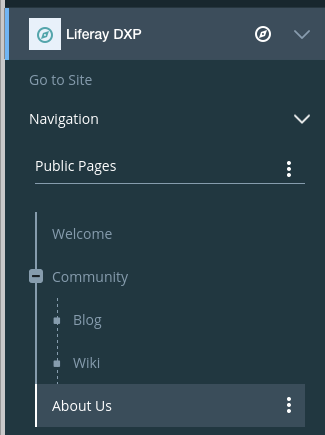
\includegraphics{./images/01-page-hierarchy.png}
\caption{Liferay's page hierarchies are easy to create, using a tree
structure that's familiar to anyone who has used a file manager.}
\end{figure}

Pages can be added, removed, or reordered any time, and you have the
full flexibility of all the HTML page attributes like meta tags and
robot file declarations, as well as full control over the layout.

Pages are also integrated with Liferay's powerful permissions system, so
it's easy to restrict access to certain portions of your site. You can
give individual users sites of their own, with public pages that have
their content and blog and private pages that contain their calendars
and profiles.

If you run a large website with lots of different sub-sites for
individuals and groups, you can use page templates and site templates.
Page templates have layouts and applications already on them, and site
template predefine a whole site made up of multiple page templates.

Web content is one example of an \emph{asset}. Assets are meta-data
attached to content types, and that meta-data aggregates similar assets
together in searches or as published content. One way to do this is to
tag and categorize content so it can be found more easily by users.

There is much more to web content. You can create structures
(pre-defined content formats), templates (designs for formatting
structures), schedule when content is published and when it should be
taken down (or reviewed), define related assets, stage multiple
variations of your site, and more.

This is just the web content portion of the content management system.
Liferay DXP is also great at managing file-based content.

\section{Keeping Track of Documents, Images, Video, and
More}\label{keeping-track-of-documents-images-video-and-more}

Liferay's file-based content management system is in an application
called \emph{Documents and Media Library}. This application, as shown
below, looks like the file manager that you're already familiar with
from your operating system.

\begin{figure}
\centering
\includegraphics{./images/01-docs-and-media.png}
\caption{Liferay DXP's Documents and Media library was purposefully
designed to be familiar to anyone who uses a computer.}
\end{figure}

Like a file manager, you can browse files and folders in nested
hierarchies. You can also mount other repositories that you might have
in your environment, such as any system that implements Content
Management Interoperability Services (CMIS). It generates previews of
many document types. And, like a file manager, you can upload, copy, and
move files between folders by dragging and dropping them. Of course, if
you still want to use your operating system's file manager you can,
because the Documents and Media library supports WebDAV, using the same
credentials you use to log in.

Liferay DXP's Documents and Media library, however, is much more robust
than a file manager is, because it's a full content management system.
You can define ways of classifying files that may be of different types,
but are meant for the same, overarching purpose.

For example,
\href{/docs/7-1/user/-/knowledge_base/u/metadata-sets}{\emph{metadata
sets}} are groups of fields describing attributes of a file. These can
be combined to define
\href{/docs/7-1/user/-/knowledge_base/u/document-types}{\emph{document
types}}. For example, you might create a document type called Meeting
Minutes. The file format doesn't matter: whether it's a Microsoft Word
document, an HTML file, or a text file, the document contains meeting
minutes.

Of course, the system goes much further than this. Folders can be set so
that only certain document types can be added to them. You can add
workflow rules to folders so files go through an approval process that
you define. In short, Liferay DXP's file-based content management system
gives you what you need to manage and share files in a group.

There are many other ways you can use Liferay DXP, starting with its
collaborative tools.

\section{Using Liferay DXP as a collaborative
platform}\label{using-liferay-dxp-as-a-collaborative-platform}

Liferay DXP includes a suite of collaborative applications, and they're
all integrated together.

These applications range from personal productivity applications like a
calendar and email, to community-building applications like message
boards, blogs, and wikis.

\begin{figure}
\centering
\includegraphics{./images/01-message-boards.png}
\caption{Liferay DXP's message boards are as fully featured as any
standalone forum application, with the added benefit that they're
integrated with the rest of the system.}
\end{figure}

This is a suite of integrated applications with all the features of
similar, standalone applications. For example, Liferay DXP's Message
Boards include categories and subcategories, message threads, captcha,
RSS feeds, email notification, posting via email, and much more. But
more than this, the applications are integrated with the rest of Liferay
DXP's framework. Users log in and their profiles are used automatically
by the message boards and all the other collaborative applications. And
as you'll see later, functionality from the built in applications can be
added to your own to provide features like comments in your own
software, and you don't have to write any code to do it.

One important feature of all the collaborative applications---as well as
web content and documents---is the Recycle Bin. If users delete content
that must be restored later, you don't have to find it in your backups:
it's in the Recycle Bin.

\begin{figure}
\centering
\includegraphics{./images/recycle-bin-overview.png}
\caption{The Recycle Bin can hold any kind of content.}
\end{figure}

Liferay DXP's suite of collaborative applications includes a Blog
(complete with blog aggregation features so you can publish multiple
users' blog entries in one place), Message Boards, a Wiki, a Knowledge
Base that you can use to publish a library of articles, activities
display, and personal productivity applications like a calendar.

Liferay DXP includes what you need to enable users to collaborate. Next,
you'll see how Liferay DXP's platform benefits developers.

\section{Using Liferay as a Development
Platform}\label{using-liferay-as-a-development-platform}

Building your site on Liferay's development platform can give you a head
start. It provides everything you need to support your applications, so
you can concentrate solely on what \emph{you're} building, and not the
rest of the features your users expect to come along with it.

Imagine your application for a moment. Does it require users to register
on your site? Can users comment on content contained in your
application? Is there something that users can tag or categorize? If you
think about how the code is organized, would it benefit from
modularization? Do you plan on having multiple clients like web and
mobile access a single back-end? Could you make use of a rich JavaScript
framework with many components built into it? How about permissions---do
you need to make information available to some users, but not to all
users?

You get all this and much more. It's a very powerful platform, and
certainly worth your investigation. If you're a developer, it behooves
you to check out our
\href{/docs/7-1/tutorials/-/knowledge_base/t/introduction-to-liferay-development}{developer
documentation}.

\subsection{A Great Integration
Platform}\label{a-great-integration-platform}

If you're building an enterprise system, portals were designed in the
first place to be a single point of entry to your users' applications
and content. Since Liferay DXP integrates with user directories such as
LDAP and Active Directory, single sign-on systems such as SAML and
OpenSSO, and authorization systems like OAuth 2.0, it fits well into
your enterprise systems. This makes it a great integration platform for
existing applications.

Liferay DXP, since it adheres to the JSR standard for portlets, was
designed from the ground up for application integration. You can add any
application installed on the system to any page. You can make use of
APIs provided by other systems to integrate their data into an
application window in Liferay. And applications you create with
Liferay's Service Builder framework can be web service-enabled from the
start.

Developing applications is only one part of the platform. Many users
value Liferay DXP for how it can be customized. Next, you'll see how you
can customize Liferay DXP so that it looks and operates exactly the way
you've envisioned for your site.

\section{Extending and customizing Liferay for your own
needs}\label{extending-and-customizing-liferay-for-your-own-needs}

Liferay DXP was specifically designed to be extended and modified,
beyond what even most open source projects provide. Though its source
code is available, Liferay DXP's developers have created many extension
points so you don't have to customize the source to make Liferay DXP
yours.

The first (and easiest) way of customizing parts of Liferay DXP is with
Application Display templates. These let you change the way built-in
applications look. For example, if you don't like the Documents and
Media Library's file manager view with large icons, you can create an
Application Display template that shows documents in some other view. If
you don't like the layout of the Blogs application, you can change it so
that it has the look you want.

Liferay DXP goes far beyond this, though. Special software components
called \emph{modules} enable developers to change Liferay's interface
and behavior without having to modify any of Liferay DXP's source code.
This provides you all the benefits of building your site from scratch,
but without all the effort to actually build from scratch. If you want
to make a change to the user registration screens, add support for a
proprietary single sign-on mechanism that you've written, add a feature
to the message boards application or anything else, you can make those
customizations. And if you're a developer, you know that it's a whole
lot easier to customize something that almost does things the way you
want than it is to write that feature from scratch.

\section{Conclusion: What Liferay DXP Really
Is}\label{conclusion-what-liferay-dxp-really-is}

So what is Liferay DXP? As you can see, it's hard to describe, because
it does so much. What we've essentially done is say it's a totally
awesome content and document managing, user collaborating, socially
enabling, application developing, corporate integrating, completely
customizable platform for building the Internet. If we'd said that up
front, you may have thought we were exaggerating. Hopefully now you can
see that we really believe it, and we continue striving to make Liferay
DXP better and better.

But please don't take our word for it.
\href{https://www.liferay.com/downloads}{Download} the open source,
Community Edition or a trial of the supported Digital Experience
Platform yourself. See how it can solve some of the problems you may be
facing. If you have questions, all the documentation is right here, you
can ask our friendly \href{https://community.liferay.com}{community} for
help, or you can contact a
\href{https://www.liferay.com/\#contact-sales}{sales representative}.

\chapter{What's New in 7.0}\label{whats-new-in-7.0}

7.0 launches new features for efficient, beautiful page design, along
with an extensive upgrade to forms. The user experience has also been
streamlined throughout the platform to help save time while managing
sites. There are new tools to support data protection in accordance with
the recent GDPR requirements. Finally, there are several significant
technology updates that help you develop new competitive advantages with
modern development tools for mobile and web.

Evolve your digital presence with new features to create stunning,
personalized experiences for every audience.

\section{Page Creation}\label{page-creation}

7.0 introduces a powerful new way to design websites. From carefully
designed page fragments to full control over page menus, Liferay DXP
frees web developers and designers to execute web experiences exactly as
they envision. This is an enhancement of the content management system
that you can adopt as you see fit. To differentiate the two, the new
pages are called Content Pages, while the existing system uses Widget
Pages.

\subsection{Content Pages}\label{content-pages}

Users can now easily create and add unstructured content directly to
pages. This is useful for site pages that don't need to leverage
structured web content, such as one-off landing pages for marketing
campaigns.

When creating a new page, users can choose either the new content pages
or widget pages, which use the traditional method of creating pages
through adding and configuring applications.

\begin{figure}
\centering
\includegraphics{./images/01-creating-pages.jpg}
\caption{Users can now choose to create Content Pages.}
\end{figure}

\subsection{Fragments}\label{fragments}

Fragments are a new way of creating and implementing content page
designs. Web developers can now save page sections as Fragments and
reuse them across a Site. Developers can now create a library of
designed components for others to build pages quickly without having to
touch code. Fragments are organized in collections and leverage familiar
asset management features such as drafts, thumbnail previews, search,
and permissions.

\begin{figure}
\centering
\includegraphics{./images/01-page-fragments.jpg}
\caption{Non-technical users can use Fragments as building blocks for
pages.}
\end{figure}

\subsubsection{Fragment Editor}\label{fragment-editor}

Web developers can use the Fragment Editor in the browser to create or
edit their Fragments. Alternatively, developers can create Fragments
with their preferred tools and import the fragments into Liferay.

\begin{figure}
\centering
\includegraphics{./images/01-fragment-editor.png}
\caption{The Fragment editor has a three-pane view for HTML, CSS, and
JavaScript, with a preview pane rendering the final result.}
\end{figure}

\subsubsection{Page Editor}\label{page-editor}

The introduction of Fragments opens up new ways to create pages and
templates through a visual page editor.

The new Page Editor is for laying out page designs visually and saving
them as reusable templates. Users can search through collections and
easily add, remove and position fragments on the page. Marketers can
then customize text with in-line editing, swapping in new images and
other elements. Fragments can display Liferay's out-of-the-box
applications, and you can configure them within the page editor.

\begin{figure}
\centering
\includegraphics{./images/01-page-editor.jpg}
\caption{The Page Editor makes it easy to build pages out of Fragments.}
\end{figure}

\subsubsection{Display Pages}\label{display-pages}

Display Pages have been improved to make it easier to create standard
templates for web content that must have a consistent look and feel,
such as press releases. Use page Fragments to implement designs and map
content sections without touching code. When web content is published
with a display page template, it automatically gets its own page with a
unique URL, replacing the default content in the template with the newly
added web content.

\subsubsection{Menus}\label{menus}

Menus are now decoupled from page navigation. Now you have the freedom
to create custom menus for sections of the site or remove marketing
landing pages from menus. You can easily manage menu hierarchies and
save different menu sets with a new drag-and-drop interface.

\begin{figure}
\centering
\includegraphics{./images/01-menus.jpg}
\caption{Menus are now decoupled from page navigation, and can be edited
independently.}
\end{figure}

\subsubsection{Forms}\label{forms}

Forms have extensive new functionality, including a set of conditional
rules that make forms dynamic: if something happens in a field, an
action elsewhere on the form can be triggered. This lets you create
calculations, offer follow-up questions based on responses, and much
more. Forms are now localized: they can be translated into any language.
There are new fields and properties, form fragments, auto-saving of
forms, and so much more it had to be
\href{/docs/7-1/user/-/knowledge_base/u/whats-new-with-liferay-forms}{described
separately}.

\begin{figure}
\centering
\includegraphics{./images/01-forms.jpg}
\caption{Forms have many improvements.}
\end{figure}

\subsubsection{User Experience}\label{user-experience}

7.0 rolls out several user experience refinements for externally facing
content such as blogs, as well as omni-channel support for how media is
displayed and delivered on different devices. These integrated
improvements help you deliver a better experience to your users out of
the box.

\subsubsection{Adaptive Media}\label{adaptive-media}

Adaptive Media dynamically adjusts images to best fit the screen size of
the device being used. It also offers deep control over how images are
loaded and displayed, which helps you address performance issues across
a wide variety of devices and varying network speeds between users and
countries. Adaptive Media does most of the work in the background
automatically, but developers can edit image resolutions and define
devices that trigger various resolutions. This level of control enables
consistent experiences that avoid poor page layouts and slow load times.

\subsubsection{Blogs and Message Boards}\label{blogs-and-message-boards}

Blog refinements make it easier to deliver experiences that are tailored
to your blog audience. These include support for creating friendly URLs,
displaying estimated reading times, unsubscribing from email
notifications, a new cards design, and support for videos from external
services. Message Boards now supports drag and drop for uploading
attachments, section renaming, category and thread grouping,
notification management, and a new design for comments.

\begin{figure}
\centering
\includegraphics{./images/01-blogs.jpg}
\caption{The new cards design for blogs displays entries in a visual
grid.}
\end{figure}

\section{Administration Improvements}\label{administration-improvements}

In addition to its new features, 7.0 is easier to administer.
Streamlined administration tools mean less time managing sites, while
still offering granular control.

\subsection{OAuth 2.0}\label{oauth-2.0}

OAuth 2.0 has become a de-facto standard that allows users to authorize
access to parts of their accounts without giving up authentication
credentials. With 7.0, now users can ``Sign in with {[}insert your site
here{]},'' granting mobile and web applications secure, token-based
access to user profile information they have complete control over and
can revoke at any time.

\subsection{Data Protection}\label{data-protection}

7.0 introduces new data protection tools to help companies address GDPR
regulations and maintain control over how their platform manages user
data.

You can now erase a user's personal data and export a user's personal
data in a machine-readable format upon request. For data erasure,
administrators can review content that potentially contains personal
information and edit or delete as needed through a simple interface.
Both tools include APIs for third-party apps to implement this feature
or override the default behavior for out-of-the-box apps.

\subsection{Search}\label{search}

7.0 improves search administration and uses Elasticsearch 6 as the
default search engine, giving users more options for implementing and
managing enterprise search for their sites.

A new Control Panel makes it easier to take care of all administration
tasks with the click of a button. Users can configure the search engine,
start and monitor re-indexes, and much more.

\begin{figure}
\centering
\includegraphics{./images/01-search.jpg}
\caption{Search administration is now separated from server
administration.}
\end{figure}

\subsection{Page Management}\label{page-management}

A new interface for visualizing and managing complex page hierarchies
makes page management easier. Page templates and display pages are now
integrated nicely, bringing page management into one central location.

\begin{figure}
\centering
\includegraphics{./images/01-new-page-management.jpg}
\caption{The new page management interface puts all page functions in
one place.}
\end{figure}

\subsection{Workflow Management}\label{workflow-management}

Workflow management
\href{/docs/7-1/user/-/knowledge_base/u/workflow\#whats-new-with-workflow}{has
received} a complete UI overhaul, with all configuration consolidated
under one area in the Control Panel. Existing workflows can now be
duplicated, definitions are versioned, and you can save drafts and
restore previous versions.

\section{Developer Improvements}\label{developer-improvements}

7.0 includes an updated collection of tools to facilitate the support
and development of Liferay projects.

\subsection{Targeting a Liferay
Platform}\label{targeting-a-liferay-platform}

Liferay Workspace helps target a specific release of Liferay DXP, so
dependencies get resolved properly. This makes upgrading your
applications easy: specify your target platform, and Workspace points to
the new version. All your dependencies are updated to the latest ones
provided in the targeted release.

\subsection{Resolving Modules Before
Deployment}\label{resolving-modules-before-deployment}

Avoid the painful process of deploying modules only to be met with
console errors or mysterious problems by resolving modules before
deployment. This can be done by calling the new \emph{resolve} Gradle
task provided by Liferay Workspace.

\subsection{7.1 Upgrade Planner}\label{upgrade-planner}

The Upgrade Planner in Liferay Developer Studio helps you upgrade your
legacy application code to Liferay DXP:

\begin{itemize}
\tightlist
\item
  Identifies code affected by the API changes
\item
  Describes each API change related to the code
\item
  Suggests how to adapt the code
\item
  Provides options, in some cases, to adapt code automatically.
\end{itemize}

\subsection{IntelliJ Support}\label{intellij-support}

Liferay development is now officially supported on IntelliJ IDEA which
offers wizards to

\begin{itemize}
\tightlist
\item
  Create a Liferay Workspace
\item
  Create projects leveraging Liferay's project templates
\item
  Create a Liferay server runtime for project deployment and debugging
\end{itemize}

\subsection{Maven Support for Blade
CLI}\label{maven-support-for-blade-cli}

Create Maven projects and Maven Liferay Workspaces using Blade CLI.

\subsection{Hybrid Mobile App
Development}\label{hybrid-mobile-app-development}

Liferay Screens 3.0 enables software developers to use Apache Cordova or
Xamarin to build cross-platform applications from one codebase designed
for the web and embed that content into a Screens app for mobile use.
Sites and applications designed for PC can be rendered in screenlets
with no additional code. The resulting apps allow native mobile
capabilities and navigation to be mixed with HTML content seamlessly.

\subsection{Modern JavaScript Frameworks
Compatibility}\label{modern-javascript-frameworks-compatibility}

Liferay DXP leverages its own npm bundler so developers can manage
dependencies between applications. 7.0 provides support for popular
JavaScript frameworks such as Angular, Vue.js, React and modern
JavaScript workflows, so that npm modules can be deployed inside of
Liferay DXP.

\subsection{Modularity Update}\label{modularity-update}

New search applications such as Search Results, Search Bar and Category
Facets allow for greater flexibility in page construction. These
applications come from the previous Search application, but have been
divided into more useful components.

The message boards services have also been modularized and extracted out
of the core, making it easier to manage and update Message Boards
independently.

\chapter{Web Experience Management}\label{web-experience-management}

Experience: consider that word for a moment. Not the type of experience
you gain with repetition, but the contact or encounter you have with
something. Suppose you're buying a new phone. It's easy to look at the
phone with the biggest screen or the fastest processor and say that it's
the best, but what will your experience be? The ``best'' phone might not
be the fastest or the biggest; it might be the phone with the longest
battery life or the most comprehensive suite of integrated apps. Or it
might not be any of those things. Experience isn't always something that
you can quantify with specs or features.

Liferay takes the experience factor very seriously when it comes to site
and content management. The Web Experience Management suite is focused
on providing the best experience for users building websites. When it
comes to web experience, just like with your phone, everyone is looking
for something different. Some smartphone users might love watching
videos during their commute with a big beautiful screen, while on the
other side, some people might be more excited about a small sleek phone
with a great battery life that fits easily in their pocket and simply
does all the basic communication they need.

Liferay's Content Management is the big beautiful phone and the sleek
utilitarian one all in one. Marketers will find easy to use tools to
build content without having to write any code or peak under the hood.
Developers will find powerful tools like Structures and Templates that
enable them to create dynamic content. And designers will love how
Fragments and Content pages provide a way to perfectly realize their
designs.

\section{Authoring Content: Structured and Inline
Content}\label{authoring-content-structured-and-inline-content}

The primary goal of Content Management isn't to show off the flashiest
new features or follow all the latest trends in design, but to provide
you with the tools you need to create digital content that communicates
your message clearly and effectively. With this in mind, Liferay offers
two core approaches to help you accelerate and simplify creating and
organizing content: Structured Web Content and Inline Content.

\subsection{Structured Web Content}\label{structured-web-content}

If you've entered content into a CMS before, you may be familiar with
the process of filling content into various fields like this:

\begin{itemize}
\item
  Title
\item
  Abstract
\item
  Text Body
\end{itemize}

This is an example of Structured Content. Structured Content is created
within a predefined content structure and then added to pages as needed.
The structure defines the fields and then a template defines its styles.
The content is then saved, ready to be added to a page later.

The structure defines what kind of content you are creating and provides
different types of fields that can be used. A developer could create a
format for publishing articles that contains a \textbf{Title},
\textbf{Header Image}, \textbf{Body Text}, and a \textbf{Key Quotation}.
The template defines how the elements of the structure are rendered. You
could style the elements in the structure with the \textbf{Title} as
large bold text, the \textbf{Header Image} as a full page width block
above the title, the \textbf{Text} as standard text, and the \textbf{Key
Quotation} as large font italics with a thin border that displays within
the main text section. A content writer or marketer could then create
any number of articles, all having a uniform style based on the
structure.

In Liferay, those articles could be added to pages across the site, or
displayed dynamically with tools like the Asset Publisher and Web
Content Display Pages.

\subsection{Inline Content}\label{inline-content}

Inline Content is content that is created directly within a page. Rather
than filling in fields to create content that's added to a page later,
you have a completed page design where you edit the text and image
content. Content Pages start with a design which is then created with
Fragments. Inside the Fragments, a developer can define where text and
images can be placed or edited. Marketers and content writers are then
free to write or add images within the page and publish it.

With content pages, basic HTML and CSS define the primary design, while
JavaScript and Liferay specific tags can add dynamic behavior to the
Content Page. After a developer creates the page and a content writer or
marketer provides the content, the content exists inline within the
page, and is published with it.

\subsection{What's best for your use
case?}\label{whats-best-for-your-use-case}

When you step back to look at the big picture, what you see are two
different paradigms for building pages: content pages, where the content
is built into the page; and widget pages, where content and other
features can be added, removed, and rearranged as desired.

Often it is helpful to have reusable elements or content that can be
moved around a page or placed anywhere on a site. For example, you might
have a content based banner which you want to be able to drop onto any
various pages with different layouts and styles, or you might have
content that uses the same template to create similar items for
different pages. Structured Content on widget pages is the tool you need
to quickly create what you need and manage these cases. Widget pages
with structured content are great for some cases, for example:

\begin{itemize}
\item
  ``Portal'' pages, where you provide users a gateway into several
  different services or providing aggregated information.
\item
  Pages where the primary focus is widgets.
\item
  Pages that are based around structured content.
\end{itemize}

In other cases, you need to create a page as a complete unit. For
example, you have a series of marketing driven landing pages that must
match a specific design and have associated content intended for use on
that page or with that campaign. Content Pages provide the best tool for
quickly bringing a design to life and empowering marketing with inline
content. Content Pages are useful for pages like:

\begin{itemize}
\item
  Landing pages
\item
  Front pages that provide marketing information or a direct path into
  the website.
\item
  Pages with multiple variations and small graphical or textual changes
  across a large number of pages.
\end{itemize}

Most sites need a little bit of both. Read on to learn more about
building sites with Liferay and how Content Pages and Structured Content
can help you do that.

\chapter{Building a Site}\label{building-a-site}

A site is a set of pages where content or applications are published.
Sites can be independent or serve as an associated organization's
website. You can create as many different sites as you like within the
context of a single Liferay instance.

You'll start with a tour of the site management user interface. Then
you'll create a custom Lunar Resort Example instance and explore ways to
create sites and pages for that Liferay instance. Finally, you'll learn
how to change various settings for sites and pages to meet your needs.
To begin building a site, continue on to the next section.

\chapter{Site Management}\label{site-management}

You can have many Sites on one Liferay instance, which work together to
create one complete website, or you can simply have one Site which
contains all of your pages and content---or anything in between. In this
section you'll look at the interface for creating and managing Sites,
create a Site, and learn how to use Site Templates for more efficient
Site creation.

\section{Understanding Site
Management}\label{understanding-site-management}

Whether you're building a large corporate webSite or a small Site for
facilitating collaboration among team members, supporting different
kinds of collaboration and social scenarios is a must. Liferay's Sites
provide three membership types:

\textbf{Open:} Users can become members of the Site at any time.

\textbf{Restricted:} Users can request Site membership but Site
administrators must approve requests for users to become members.

\textbf{Private:} Users cannot join the Site or request Site membership.
Site administrators must manually select users and assign them as Site
members.

In addition to these memberships, when a Site is associated with an
organization, all the users of that organization are automatically
considered members of the Site.

You can view all the available open and restricted Sites by adding the
My Sites application to a page and accessing the \emph{Available Sites}
tab. You can request access to any of the Sites you're not already a
member of by selecting the Site's \emph{Options} button

(
\includegraphics{./images/icon-actions.png}) and clicking \emph{Join}.

\subsection{Site Scope}\label{site-scope}

Members of a Site can be given additional privileges in the Site by
using permissions. It is also possible to assign different roles within
the Site to different members. This can be done through \emph{Site
Roles}, which are defined equally for all Sites or \emph{Teams} which
are unique for each Site. These concepts are discussed later.

Liferay DXP separates Site-scoped information from the Control Panel by
placing it in the Site menu. From this menu, you can select the specific
Site to work on. The Site Administration panel is available for your
Site, which includes Build, Content, Categorization, Recycle Bin,
Members, Configuration, and Publishing.

\begin{figure}
\centering
\includegraphics{./images/web-content-site-content.png}
\caption{Your Site's content resides in the Site Administration menu.}
\end{figure}

\subsection{Site Hierarchies}\label{site-hierarchies}

Sites can also be organized hierarchically, just like Organizations. The
difference between Sites and Organizations, of course, is that Sites
organize pages, content, application data, and users (via Site
memberships) whereas organizations only group users. Content sharing is
available for Sites within the same hierarchy. For instance, if a parent
Site has a document type called \emph{Lunar Presentation} and all its
child Sites should have a copy, the parent Site's administrator can
enable content sharing to share the document type automatically with its
child Sites. Also, content sharing privileges can be set to let every
Site administrator share content across Sites they manage. You can share
the following content across Sites:

\begin{itemize}
\tightlist
\item
  Web Content Structures
\item
  Web Content Templates
\item
  Document Types
\item
  Vocabularies and Categories
\item
  Widget Templates
\item
  Data Definitions (Dynamic Data Lists)
\end{itemize}

Please refer to the
\href{https://docs.liferay.com/dxp/portal/7.1-latest/propertiesdoc/portal.properties.html\#Sites\%20Admin\%20Portlet}{Sites
Admin Portlet} section of Liferay's \texttt{portal.properties} file for
a list of relevant configurable properties. For example, the
\texttt{Sites.content.sharing.with.children.enabled} property can
disable content sharing between Sites and child Sites, disable it by
default while allowing Site administrators to enable it per Site, or to
enable it by default while allowing administrators to disable it per
Site.

The Sites Directory application is a configurable app that shows a
hierarchy of Sites and child Sites. It enables users to navigate to any
of the displayed Sites. To use this app to display Site hierarchies, add
it to a page, open its Configuration window, and under Display Style,
select \emph{List Hierarchy}. The My Sites Directory application is
similar to the Sites Directory application, except that it lists only
the Sites a user belongs to.

Each child Site in the hierarchy has its own administrator, and the Site
Administrator role permissions do not flow down to child Sites in the
hierarchy. If a Site Administrator creates a child Site, he or she has
the same permissions in that child Site. This is not, however, because
of inheritance. It is only because creating a Site makes you the Owner
of that Site. A Site Administrator or a parent Site has no default role
in any child Sites created by other Site Administrators.

If you wanted a user to have administrative access to all Sites in a
Site/child Site hierarchy, you must create a role based on the Site
Administrator role that has the permission \emph{Manage SubSites}.

The Site Map application helps users navigate a Site. A Site
administrator can configure a root page and a display depth. Just as
Sites can have hierarchies, so can the pages within a Site. The display
depth of the Site Map application determines how many levels of nested
pages to display.

\begin{figure}
\centering
\includegraphics{./images/site-directory-site-map.png}
\caption{The Site Map application lets users navigate among pages of a
Site organized hierarchically.}
\end{figure}

\subsection{Site Members}\label{site-members}

Another useful administrative application is the Site Members
application. This enables administrators to survey all the users,
organizations, and user groups that reside in the Site. Similarly,
Liferay provides the Portal Directory application, which functions the
same as the Site Members app, but globally scoped for all Sites in the
instance.

\subsection{Page Sets}\label{page-sets}

Sites have two categories of pages called page sets. There are two kinds
of page sets: public pages and private pages. A Site can have only
public pages, only private pages, or both. Private pages can only be
accessed by Site members. Public pages can be accessed by anyone,
including users who haven't logged in. It's possible to restrict access
to pages at the page set level or at the level of individual pages
through the permissions system. Public pages and private pages have
different URLs and can have different content, applications, themes, and
layouts.

Building a corporate intranet is a typical use case for Sites. A
corporate intranet could have Sites for all the organizations in the
company: Sales, Marketing, Information Technology, Human Resources and
so on. But what about the corporate health and fitness center? That's
something everybody in the company, regardless of organization, may want
to join. This makes it a good candidate for an open and independent
Site. Similarly, the home page for a corporate intranet should probably
be placed in an open independent Site so any member of the instance can
access it.

For other kinds of websites, you may want to use independent Sites to
bring users together who share a common interest. If you were building a
photo sharing website, you might have independent Sites based on the
types of photos people want to share. For example, those who enjoy
taking pictures of landscapes could join a Landscapes Site and those who
enjoy taking pictures of sunsets could join a Sunsets Site.

There is always one default Site, which is also known as the main Site
of the instance. This Site does not have its own name but rather takes
the name of the instance. By default the instance name is \emph{Liferay}
but this value can be changed through the configuration of the setup
wizard. The instance name can also be changed at any time through the
Control Panel within \emph{Configuration → }Instance Settings*.

\section{Adding Sites}\label{adding-sites}

Sites can be created through the Control Panel by a Liferay
administrator. The Control Panel provides an administrative interface
for managing your Liferay instance. There are four main sections of the
Liferay Control Panel: Users, Sites, Apps, and Configuration. In this
section, you'll learn how to use the Control Panel to manage Sites. For
information about the Apps, Users, and Configuration sections of the
Control Panel, see the
\href{/docs/7-1/user/-/knowledge_base/u/using-the-liferay-marketplace}{Using
the Liferay Marketplace},
\href{/docs/7-1/user/-/knowledge_base/u/managing-users}{Managing Users},
and \href{/docs/7-1/user/-/knowledge_base/u/system-wide-settings}{System
Wide Settings} sections, respectively.

\noindent\hrulefill

\textbf{Tip:} If you're signed in as an administrator, you can access
all Sites by navigating to the Site Administration menu from the Control
Panel. To manage a single Site, navigate to the Site by going to the
Menu and clicking the \emph{Site Selector} button
(\includegraphics{./images/icon-compass.png}) from the Sites dropdown
menu and selecting the appropriate Site name. Once finished, the Site
administration options (i.e., Navigation, Content, Members, etc.) for
that Site are available.

\noindent\hrulefill

Now, you'll add a Site for the Lunar Resort.

\begin{enumerate}
\def\labelenumi{\arabic{enumi}.}
\item
  Navigate to the Control Panel and select \emph{Sites} → \emph{Sites}.
\item
  Click the Add icon (
\includegraphics{./images/icon-add.png}) at the
  top right of the page.
\item
  Select a \emph{Blank Site}.

  Any available Site templates appear for you to select. Site templates
  provide a preconfigured set of pages, applications, and content that
  can be used as the basis of a Site's public or private page set. To
  create a Site from scratch, select \emph{Blank Site}. Otherwise,
  select the name of the Site template you want to use. If you opt to
  create a Site from a Site template, you have to choose whether to copy
  the Site template's pages as your new Site's public or private page
  set. If other Site templates are created, they will appear in the Add
  menu as they become available.
\item
  Name your Site ``The Lunar Resort''
\end{enumerate}

After you enter the name, you will be prompted to enter additional
information about the Site and configure certain Site settings.

\textbf{Name:} names the Site you wish to create. You also have the
option to translate the name for many different languages. This can be
done by selecting the language flag under the Name field, and inserting
the name in the selected language. Liferay saves the name translation
for each language and displays the translated Site name when that
specific language is selected for the instance. If a name translation is
not provided, the default instance language's name is displayed.

\textbf{Description:} describes the Site's intended function. The
description can also be translated to other languages; see the Name
description for more information on translating the Site's description.

\textbf{Active:} determines whether a Site is active or inactive.
Inactive Sites are inaccessible but can be activated whenever a Site
administrator wishes.

\textbf{Membership Type:} can be open, restricted, or private. An open
Site appears in the My Sites app and users can join and leave the Site
whenever they want. A restricted Site is the same except users must
request membership. A Site administrator must then explicitly grant or
deny users' requests to join. A private Site does not appear in the My
Sites app and users must be added to it manually by a Site
administrator.

\textbf{Allow Manual Membership Management:} determines whether to allow
or disallow users to be manually added or removed from the Site. By
default, manual Site membership management is enabled. This allows
administrators to manually assign users to the Site. It also allows
users to join open Sites or request membership from restricted Sites
using the My Sites app. For organization Sites, manual Site membership
management is disabled, by default. This causes organization members to
be automatically assigned membership following the organization's
membership policy. Also, because manual membership management is
disabled for organization Sites, by default, the \emph{Users} section of
\emph{Sites} is unavailable. To activate the \emph{Users} functionality
for your organization Site, you'll need to check \emph{Allow Manual
Membership Management} after creating the organization Site by
navigating to its \emph{Site Settings} menu.

\noindent\hrulefill

\textbf{Note:} It's possible for Site memberships to be handled
automatically by a membership policy. The membership policy can check
various pieces of information from each user, such as their first names,
last names, birthdays, job titles, organizations, and user groups. Using
this information, the Site membership policy can automatically assign
members to the Site. If your Site will implement a membership policy,
your Site administrators can disallow manual membership management for
their Site. When the Allow Manual Membership Management option is
disabled, the \emph{Members} section of Site Administration (Site
Memberships and Site Teams) is hidden, even from administrators.

\noindent\hrulefill

\textbf{Parent Site:} lets you select a parent Site for the Site that's
being created. Sites can be organized hierarchically. Using hierarchical
Sites provides a simplified way to manage Site memberships and Site
content sharing. For organizations that have attached Sites, the
organization hierarchy should match the Site hierarchy. When you select
a parent Site, an additional option appears: \emph{Limit membership to
members of the parent Site}. If this option is enabled, the Site's
membership policy performs a check so that you can only assign members
to the current Site if they're already members of the parent Site.

\begin{enumerate}
\def\labelenumi{\arabic{enumi}.}
\setcounter{enumi}{1}
\item
  Set the \emph{Membership Type} as \emph{Restricted}.
\item
  Leave the remain defaults and click \emph{Save}.
\end{enumerate}

When creating a blank Site or organization Site, the Site is not
immediately viewable. This is because Sites without a page are
impossible to view. Therefore, before you can view your Site, you must
first create a page for it. To add a page for your temporarily invisible
Site, navigate to the \emph{Navigation} option from Site Administration.
Then add a public page. After adding your Site's first page, it renders
and your Site is viewable. For more information about adding pages, see
the
\href{/docs/7-1/user/-/knowledge_base/u/creating-and-managing-pages}{Creating
and Managing Pages} section.

You can also categorize your Site template using tags and categories by
selecting the \emph{Categorization} menu from the bottom of the page. To
learn more about using tags and categories in Liferay, see the
\href{/docs/7-1/user/-/knowledge_base/u/organizing-content-with-tags-and-categories}{Organizing
Content with Tags and Categories} section. Lastly, at the top of the
page is an additional tab named \emph{Social}. This tab manages whether
users of your Site can mention other users. You'll learn about
mentioning users later in the Social Collaboration sections.

When creating a Site from a Site template, you're asked if you want to
copy the pages from the template as public pages or as private pages. By
default, the Site is linked to the Site template and changes to the Site
template propagate to any Site based on it. A checkbox appears for
unlinking the Site template if the User has permission to do so.

Once the Site has been created, you should configure its settings to fit
your needs. You can learn more about Site Settings in
\href{/docs/7-1/user/-/knowledge_base/u/configuring-sites}{Configuring
Sites}.

Next, you'll learn about creating pages.

\chapter{Adding Pages to Sites}\label{adding-pages-to-sites}

In the previous section, you learned how to create sites. You may have
gathered from that section that sites aren't particularly useful without
pages. In fact, sites primarily exist for the sake of organizing pages
and content, so now you'll learn about the different types of pages in
Liferay, and how to select the best tools based on your use cases.
You'll also learn how to manage pages and use various configuration
options.

\section{Creating Pages}\label{creating-pages}

After you create a Site, you can add new pages and maintain them. You
can do everything you need with pages from Site Administration.

\begin{enumerate}
\def\labelenumi{\arabic{enumi}.}
\item
  If you're not currently on the Site you want to edit, click the
  \emph{Site Selector} button
  (\includegraphics{./images/icon-compass.png}) next to your current
  Site name in the Menu and select your desired Site.
\item
  Go to \emph{Site Administration} → \emph{Build}.
\item
  Click on \emph{Site Pages}
\end{enumerate}

\begin{figure}
\centering
\includegraphics{./images/managing-site-pages.png}
\caption{The Sites Pages page allows you to edit your Site pages as a
whole.}
\end{figure}

From here, you'll create pages and page templates.

\noindent\hrulefill

Note: Pages are always part of page sets, and page sets are always
associated with Sites. Even users' personal pages are part of their
personal Sites. All pages belong to one of two types of page sets:
public pages and private pages. By default, anyone can access public
pages, even non-logged in users (guests). Only users who are members of
the Site that owns the pages can access private pages. This means the
private pages of an organization's Site are viewable only by Site
members and members of the organization.

\noindent\hrulefill

From \emph{Site Pages} you can do several things:

\begin{enumerate}
\def\labelenumi{\arabic{enumi}.}
\item
  Click the \texttt{+} button in the top right corner to add a new page.
\item
  Click options icons manage page or page set settings.
\item
  Create child pages by clicking the \texttt{+} button next to an
  existing page.
\end{enumerate}

\begin{figure}
\centering
\includegraphics{./images/site-pages-breakdown.png}
\caption{Understanding the options on Site Pages.}
\end{figure}

Adding a child page creates child pages in the hierarchy below the page
you've selected. You can nest pages as deep as you like.

\noindent\hrulefill

\textbf{Note:} You're not forced to define the page hierarchy in a
page's friendly URL. Therefore, child page friendly URLs are not
required to include their parent page. For example, a parent page named
Parent and its child page named Child could have the URLs
\emph{SITE\_URL/parent} and \emph{SITE\_URL/child}, respectively. The
default friendly URL given to a page is based only on the page name and
not the hierarchy. If you wish to modify a generated friendly URL, you
can do so by following the
\href{/docs/7-1/user/-/knowledge_base/u/individual-page-settings\#name-and-friendly-url}{Friendly
URL} configuration section.

\noindent\hrulefill

Once you've clicked the \texttt{+} icon to add a page, you're asked to
select the type of page you are creating. There are two top options
followed by other page types:

\textbf{Widget:} Creates a page with a layout template that defines a
number of rows and columns for adding widgets to your page.

\textbf{Content:} Creates a Content Page with inline editing based on
Fragments.

Below those you have other options:

\textbf{Full Page Application:} Creates a page that displays a single
full page application.

\textbf{Page Set:} Creates a container for subpages that is not actually
a page itself.

\textbf{Link to a Page of this Site:} Links to a page within the same
Site. This is often used to make a page available in multiple parts of a
Sites hierarchy.

\textbf{Panel:} A page containing any number of applications as selected
by an administrator, but only one is displayed at a time. Users select
the portlet they want to use from a menu on the left side of the page,
and the selected portlet takes up the entire page.

\textbf{Embedded:} Displays content from another website inside your
instance. An administrator can set a URL from the page management
interface and that page appears in the context and within the navigation
of your Liferay instance. To embed an external website, you must provide
the protocol in the URL (e.g.~\texttt{https://www.liferay.com/}).

\textbf{Link to URL:} Creates a link to any URL. This could be an
external page or a link across Sites in the same Liferay instance.

To the left, under Collections, you can choose to view the basic page
types or a collection of page templates. By default, only \emph{Global
Templates} appears, but additional collections you create appear here as
well.

\begin{figure}
\centering
\includegraphics{./images/page-types-adding.png}
\caption{You must select a page type when adding pages.}
\end{figure}

After you've added a page, it may be difficult to track what kind of
page you're currently viewing. The page type appears at the top of the
page to help you determine the administration options you have and where
you need to go to configure the page.

\begin{figure}
\centering
\includegraphics{./images/page-type-guide.png}
\caption{Here are three different page with three different types as
they as displayed in the heading.}
\end{figure}

Now that you know the basics of adding pages, you can start working on
the Lunar Resort Site. If you're not currently on the right Site,
navigate to Site Administration in the Menu, select the compass icon
next to the current Site name, and select the Site you wish to edit.

If you must ever modify the page you've created for your Site, select
\emph{Configure} from the Options menu for the page from \emph{Site
Pages}. When configuring a specific page, you have more options than
when you were creating a new page. You can also read
\href{/docs/7-1/user/-/knowledge_base/u/configuring-sites}{Configuring
Sites}.

There are also configuration options that are only available for
individual pages or page groups only. You'll learn about options
available for both instances.

Next, you'll look at creating the main page types you'll use in Liferay.

\chapter{Page Types and Templates}\label{page-types-and-templates}

Each page type has unique features that fit together to create
compelling sites. Here you'll look at each type in more detail, with a
focus on the three most common page types: Layout Pages, Content Pages,
and Full Page Applications. Since Page Templates are integral creating
pages, you'll also learn about Page Templates and how to create and use
Page Templates for different kinds of pages.

\chapter{Using Content Pages}\label{using-content-pages}

Content Pages are new in 7.0. They provide a way to create pages with
inline content. Traditionally in Liferay, all content has lived outside
the page, to be added to any page as needed. With Content Pages, you can
create a design on a page and then edit text or images directly within
the page without any abstraction between the page and the content.

!P\href{https://portal.liferay.dev/documents/113763090/113919826/vid-building-content-pages-thumbnail.png}{Video
Thumbnail}

The process starts with a design. After the design is completed, a
developer creates Fragments based on those designs. Widgets can be
embedded in Fragments. Fragments can then be converted into Page
Templates. Developers can define areas of Fragments to have editable
text or images, allowing changes during the final publication process
for the page.

This means that Fragments can be created as completely static elements
to be used to build a Content Page, or marketers and content creators
can customize them, using the Fragment as a tool for creating beautiful
content.

!V\href{https://portal.liferay.dev/documents/113763090/113919826/building-content-pages-with-fragments.mp4\%7Chttps://portal.liferay.dev/documents/113763090/113919826/building-content-pages-with-fragments.webm}{Video
Tutorial}

\section{Creating Page Fragments}\label{creating-page-fragments}

To create Content Pages, you must first have some Fragments. Fragments
are one of the building blocks that you can use to create rich content
in Liferay. Fragments are intended to be created by developers as they
are built using HTML, CSS, and JavaScript.

\subsection{Creating and Managing
Fragments}\label{creating-and-managing-fragments}

Start in Site Administration. You can find Fragments in the Content
section.

\begin{enumerate}
\def\labelenumi{\arabic{enumi}.}
\item
  Open the main menu.
\item
  Under \emph{Site Administration}, make sure the Site where you want to
  work is selected.
\item
  In the \emph{Build} section, select \emph{Page Fragments}.
\end{enumerate}

\begin{figure}
\centering
\includegraphics{./images/empty-fragments-page.png}
\caption{Here is the Page Fragments page with no Fragments or
Collections created.}
\end{figure}

Fragments are organized in \emph{Collections}. The main Page Fragments
page shows available Collections, provides the option to Import and
Export, and enables you to create Collections. You can also manage the
organization and display of Fragments and Collections once you have them
created. To create a Fragment, you must first create a Collection.

\begin{enumerate}
\def\labelenumi{\arabic{enumi}.}
\item
  Click \emph{New} → \emph{Collection} to add a Collection.
\item
  Give the Collection a \emph{Name} and \emph{Description} and click
  \emph{Save}.
\end{enumerate}

Collections help you organize Fragments, and can be used to
differentiate between different types of Fragments or Fragments used by
different groups or departments. Next you want to create a Fragment
inside the Collection you created.

\begin{enumerate}
\def\labelenumi{\arabic{enumi}.}
\item
  Click on the Collection you created.
\item
  Click the \emph{Add} icon ( 
\includegraphics{./images/icon-add.png})
  to create a Fragment.
\item
  Give it a \emph{Name} and click \emph{Submit}.
\end{enumerate}

Now you're looking at the Fragment development environment. Each pane in
the editor has a different function:

\begin{itemize}
\tightlist
\item
  The top left pane is for entering HTML.
\item
  The top right pane is for entering CSS.
\item
  The bottom left pane is for entering JavaScript.
\item
  The bottom right pane provides a live preview as you work in the other
  panes.
\end{itemize}

\begin{figure}
\centering
\includegraphics{./images/fragments-editor.png}
\caption{The Fragments editor provides an environment for creating all
the parts of a Fragment.}
\end{figure}

In addition to standard HTML, CSS, and JavaScript, developers can also
embed widgets and provide fields with editable text and images. The text
and images can be edited during the final Content Page publication
process. Fragment development is covered in depth in
\href{/docs/7-1/tutorials/-/knowledge_base/t/developing-fragments}{Developing
Fragments}.

After some Fragments have been created and published, you can start
creating Page Templates to combine Fragments into pages.

\section{Building Content Pages from
Fragments}\label{building-content-pages-from-fragments}

After Page Fragment collections are published, you are ready to create
Page Templates. A Page Template is composed of some number of
Fragments---one or fifty; it doesn't matter.

\subsection{Creating a Page Template}\label{creating-a-page-template}

You create Page Templates in the \emph{Pages} page in Site
Administration.

\begin{enumerate}
\def\labelenumi{\arabic{enumi}.}
\item
  From Site Administration for your Site, go to \emph{Build} →
  \emph{Pages}.
\item
  Select the Page Templates tab. Like Fragments, Content Page Templates
  must be created in Collections. Your Collections appear on the Page
  Templates page.
\item
  Click the \emph{New} button to add a Collection.
\item
  \emph{Name} your Collection, provide a \emph{Description}, and click
  \emph{Save}.
\item
  Click on the new Collection.
\item
  Click the \emph{Add} icon ( 
\includegraphics{./images/icon-add.png})
  and select \emph{Content Page Template} from inside the Collection.
\item
  Set the \emph{Name} and click \emph{Submit}.
\end{enumerate}

Now you're on the Page Template creation page. Fragments are added by
selecting a Collection from the \emph{Fragments} tab on the right and
adding them to the page. You can add multiple Fragments from different
collections, and you can add the same Fragment to the page multiple
times. To see the Fragments that comprise the current page, you can
check the \emph{Added} tab. The template is automatically saved as you
work, but you must click \emph{Publish} to make it available for use.

\begin{figure}
\centering
\includegraphics{./images/content-page-template-creation.png}
\caption{Drag Fragments to create a Page Template.}
\end{figure}

If the template contains editable text, you can click on the editable
text area to change the text.

\begin{figure}
\centering
\includegraphics{./images/edit-text-inline.png}
\caption{Editing text in-line lets you customize what's on the
template.}
\end{figure}

If the template contains an editable image, you can click on the image
and replace it by uploading your own image or selecting one from
Documents and Media.

\begin{figure}
\centering
\includegraphics{./images/edit-image-inline.png}
\caption{When you mouse over an editable image, a blue outline appears.
You can replace it by clicking on it.}
\end{figure}

\noindent\hrulefill

Note: While creating Page Templates, you can change editable Fragments.
While creating the final Content Page, you can make changes to the Page
Template. Changes you make to the Fragment for a Page Template are only
reflected in that Page Template, and don't affect the Fragment itself.
Likewise, when you apply edits to the text or images of a Content Page,
those changes only exist on the current page and not on the Page
Template itself.

\noindent\hrulefill

Click on the back arrow at the top to stop editing the template.

\subsection{Creating a Content Page}\label{creating-a-content-page}

When you're finished creating a Page Template, you can use that template
to create a Content Page. A Content Page is a page created from
Fragments. Any attributes of the page that were defined by the developer
as editable can be edited during the creation of the page or page
template.

\begin{enumerate}
\def\labelenumi{\arabic{enumi}.}
\item
  Go back to \emph{Build} → \emph{Pages}.
\item
  Click the \emph{Add} icon ( 
\includegraphics{./images/icon-add.png})
  for \emph{Add Page} and select \emph{Public Page}.
\item
  Select the Collection that contains the template you want to use from
  the \emph{Collections} menu on the left.
\item
  Click on the template you want to use.
\item
  Enter a \emph{Name}.
\item
  Click \emph{Save}.
\end{enumerate}

The page is published immediately, but you can edit the final page. You
can change the chosen Fragments and edit any editable fields so that the
final page is different from the Page Template.

\begin{figure}
\centering
\includegraphics{./images/selecting-template.png}
\caption{Selecting you page template.}
\end{figure}

Alternatively, you can create a Content Page without a template. From
the page creation screen,

\begin{enumerate}
\def\labelenumi{\arabic{enumi}.}
\item
  Select \emph{Basic Pages} from under \emph{Collections}.
\item
  Select \emph{Content Page}.
\item
  Enter a \emph{Name} and click \emph{Save}.
\item
  Add Fragments to create your new page.
\end{enumerate}

By default, your new page is added to the Navigation Menu and users can
access the page you created.

\noindent\hrulefill

Note: While portlets are rendered according to
\href{https://docs.liferay.com/ce/portal/7.1-latest/definitions/liferay-portlet-app_7_1_0.dtd.html\#render-weight}{\texttt{render-weight}}
on Widget Pages, that is not true for Content Pages. Portlets are
rendered in the order they appear on the page on Content Pages
(i.e.~left to right, top to bottom).

\noindent\hrulefill

\subsection{Propagation of Page Fragment
Changes}\label{propagation-of-page-fragment-changes}

If you make an update to a Page Fragment or Content Page Templates it
doesn't automatically propagate changes, but you can access the
\emph{Usages and Propagation} page to selectively propagate changes.

\begin{enumerate}
\def\labelenumi{\arabic{enumi}.}
\item
  From the Site Configuration menu, go to \emph{Build} → \emph{Page
  Fragments}
\item
  Select the Collection containing the changed fragment.
\item
  Open the menu for the fragment and select \emph{View Usages}.
\end{enumerate}

\begin{figure}
\centering
\includegraphics{./images/fragment-view-usages.png}
\caption{Select \emph{View Usages} to propagate fragment changes.}
\end{figure}

The \emph{Usages and Propagation} Page shows a list of every Page, Page
Template, and Display Page that uses the selected Page Fragment. You can
then selectively propagate fragment changes to any or all of the pages
listed. You can use the various filters and selection options to apply
updates to pages quickly.

\begin{figure}
\centering
\includegraphics{./images/fragment-usages-and-propagation.png}
\caption{Viewing the Usages and Propagation page.}
\end{figure}

To update a page or template,

\begin{enumerate}
\def\labelenumi{\arabic{enumi}.}
\item
  Select the page or pages you want to update by checking the box next
  to the page name.
\item
  Click the \emph{Propagate} icon (
  \includegraphics{./images/icon-propagate.png})
\end{enumerate}

After you propagate changes, visit any effected pages to verify there
were no unexpected side effects of the changes. Changes to existing
\texttt{editable} fields are not propagated since this overwrites
content currently in content pages. To force propagation to content in
an \texttt{editable} field, a developer must change the field ID. Any
content created in that field will no longer display in the Content Page
when the changes are propagated, but it will remain in the database and
can be retrieved using the old ID.

Next you'll learn how to import and export Page Fragments.

\section{Exporting and Importing
Fragments}\label{exporting-and-importing-fragments}

Often you'll want to reuse Fragments or re-purpose some of the code from
Fragments in another Site or somewhere else altogether. Since all the
content is plain text, copy/pasting your code would always be an option,
but there's provides a much more elegant solution: exporting your
Fragment Collections.

\subsection{Exporting Fragments}\label{exporting-fragments}

There are two ways to export Fragments:

\begin{enumerate}
\def\labelenumi{\arabic{enumi}.}
\item
  Export a single Collection.
\item
  Export some Fragments outside of a Collection.
\end{enumerate}

To export a single Collection,

\begin{enumerate}
\def\labelenumi{\arabic{enumi}.}
\item
  Go to \emph{Site Administration} → \emph{Build} → \emph{Page
  Fragments}.
\item
  Next to \emph{Collections} click \emph{Actions}
  (
\includegraphics{./images/icon-actions.png}) and select
  \emph{Export}.
\item
  Select a Collection or multiple Collections to be exported. Each
  collection exports in a separate file.

  \begin{figure}
  \centering
  \includegraphics{./images/collections-export.png}
  \caption{Select Collections to export.}
  \end{figure}
\end{enumerate}

Each Collection \texttt{.zip} contains all data for the Collection as
well as the Fragments within it.

To export individual Fragments,

\begin{enumerate}
\def\labelenumi{\arabic{enumi}.}
\item
  Click on the Collection that you want to export the fragment from.
\item
  To export all Fragments in the Collection without exporting any
  Collection data, click \emph{Actions}
  (
\includegraphics{./images/icon-actions.png}) \emph{Export} next to
  the Collection name. A \texttt{.zip} file is generated and downloaded
  automatically.

  \begin{figure}
  \centering
  \includegraphics{./images/fragments-export-individual.png}
  \caption{Exporting all of the Fragments in a Collection.}
  \end{figure}
\item
  To export a single Fragment, click \emph{Actions}
  (
\includegraphics{./images/icon-actions.png}) \emph{Export} next to
  the Fragment. A \texttt{.zip} file is generated and downloaded
  automatically.
\end{enumerate}

When you export a single Fragment or a group of Fragments without a
collection, you must have an existing Collection to import them into.

Now that you've done all this exporting, it's time to import it all back
it.

\subsection{Importing}\label{importing}

There are a few options for importing fragments, depending on how you
exported them. You can import a Collection that was created in Liferay
DXP, a Collection created using external tools, or any number of Page
Fragments without a collection. Any time you import any Page Fragments
they aren't available for use until you have gone to each imported
fragment and approved it for use. This is to ensure that there are no
errors in any imported fragments before they are added to a page.

See
\href{/docs/7-1/tutorials/-/knowledge_base/t/recommendations-and-best-practices\#developing-a-fragment-using-desktop-tools}{Developing
a Fragment Using Desktop Tools} for more information on creating and
importing Fragments using other tools.

\subsubsection{Importing Collections}\label{importing-collections}

You can import collections that were exported from Liferay DXP or that
were created using other tools. To import a collection, follow these
steps:

\begin{enumerate}
\def\labelenumi{\arabic{enumi}.}
\item
  Go to \emph{Site Administration} → \emph{Build} → \emph{Page
  Fragments}.
\item
  Next to \emph{Collections}, click \emph{Actions}
  (
\includegraphics{./images/icon-actions.png}) and select
  \emph{Import}.

  \begin{figure}
  \centering
  \includegraphics{./images/collections-import.png}
  \caption{Importing and exporting Collections is accessed from a single
  menu.}
  \end{figure}
\item
  On the next screen, click \emph{Choose File} and select the file you
  want to import.
\item
  If you want to replace an existing collection, make sure the box is
  checked for \emph{Overwrite Existing Files}.
\item
  Click \emph{Import} and the collection is uploaded.
\end{enumerate}

\subsubsection{Importing Individual Page
Fragments}\label{importing-individual-page-fragments}

You can also import a single Page Fragment or a set that was exported
outside of a collection.

\begin{enumerate}
\def\labelenumi{\arabic{enumi}.}
\item
  From the root level of the Fragments page, click on an existing
  Collection where you want to import the Fragments.
\item
  From inside the Collection click the \emph{Actions}
  (
\includegraphics{./images/icon-actions.png}) button in the top right
  corner of the page.
\item
  Select \emph{Import}.
\item
  Drag-and-drop or click \emph{Select} to upload the Fragments
  \texttt{.zip}.
\item
  Click \emph{Import}
\end{enumerate}

The Fragments are imported into the Collection where you performed the
import.

Export and Import let you use your preferred developer tools or share
Fragment functionality elsewhere.

\chapter{Using Widget Pages}\label{using-widget-pages}

Widget Pages are composed of ``widgets.'' A widget is any application
that you can add to a page. Widget Pages are constructed by adding
widgets to the page and filling them with content.

A widget could be a wiki display or a dynamic publishing tool like the
Asset Publisher. The content you display with widgets could be long-form
text or an image gallery, or anything in between. In this section,
you'll learn to create widget pages and build content with them.

\section{Creating Widget Pages}\label{creating-widget-pages}

Widget Pages are the classic type of page in Liferay DXP. They're simple
to create and fill with content or functionality. You create a blank
page, define a layout, and then add widgets to the layout. Widgets can
display content or provide some tool or function for Users.

\subsection{Adding a Widget Page}\label{adding-a-widget-page}

When you first start Liferay DXP you get a widget page by default as
your home page. To create a new widget page,

\begin{enumerate}
\def\labelenumi{\arabic{enumi}.}
\item
  Go to \emph{Site Administration} → \emph{Build} → \emph{Pages}.
\item
  Click the \emph{Add} icon ( 
\includegraphics{./images/icon-add.png})
  in the top right and select \emph{Public Page} to add a new page.
\item
  Select \emph{Basic Pages} if it is not selected by default.
\item
  Select the \emph{Widget Page} type.
\item
  Name the page \emph{Community} and leave the box checked to \emph{Add
  this Page to the following Menus: Default}.
\item
  Click \emph{Submit}.
\item
  On the next screen, you can select a Layout Template or manage other
  options. Leave the defaults and click \emph{Save}.
\end{enumerate}

\begin{figure}
\centering
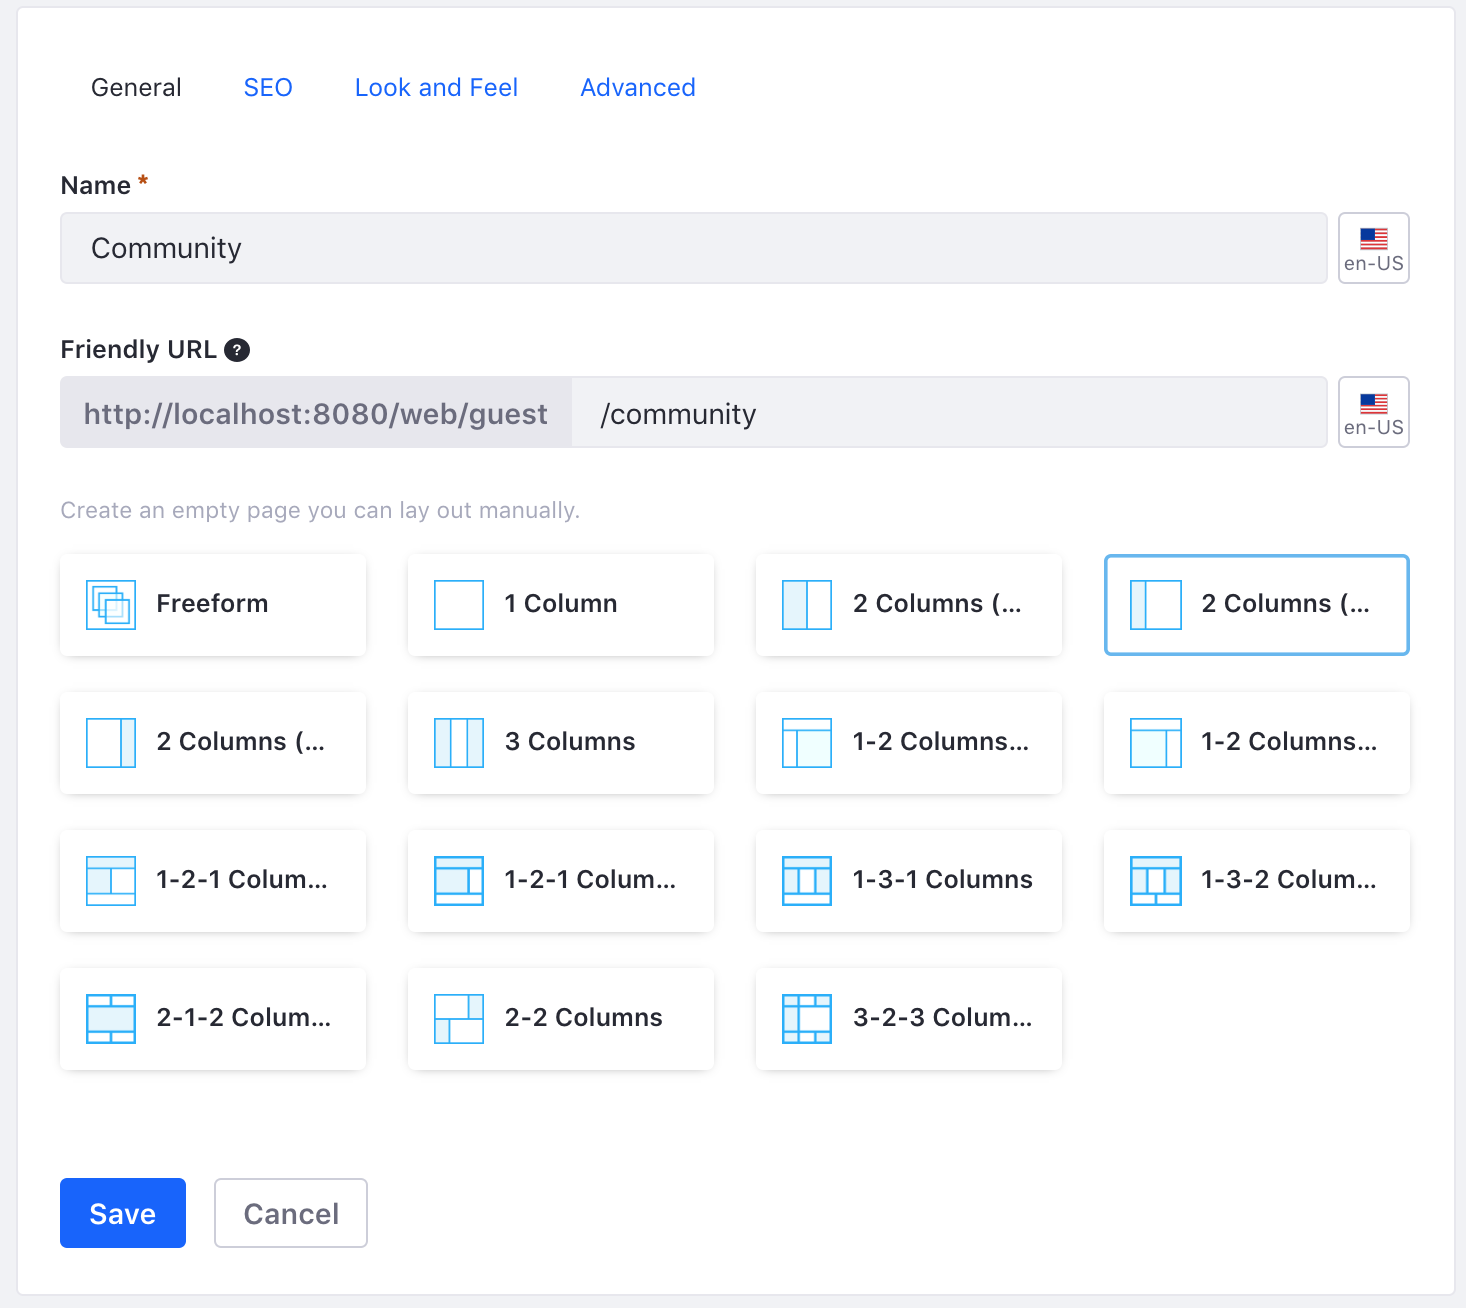
\includegraphics{./images/creating-community-page.png}
\caption{Create a page called \emph{Community} with two columns.}
\end{figure}

Creating a page by default also adds it to any Navigation Menus that are
configured to have new pages added to them. If you don't want a new page
added to a specific Navigation Menu that is listed during page creation,
uncheck the box for that menu.

Your new page is now added to the navigation.

\begin{enumerate}
\def\labelenumi{\arabic{enumi}.}
\item
  Click the logo in the top left of the page to go back to your Site's
  front page. The page you just created appears in the main navigation.
\item
  Click on \emph{Community} to go to the page.
\end{enumerate}

Currently the page is empty. Next you'll add some widgets to give it
functionality.

\begin{figure}
\centering
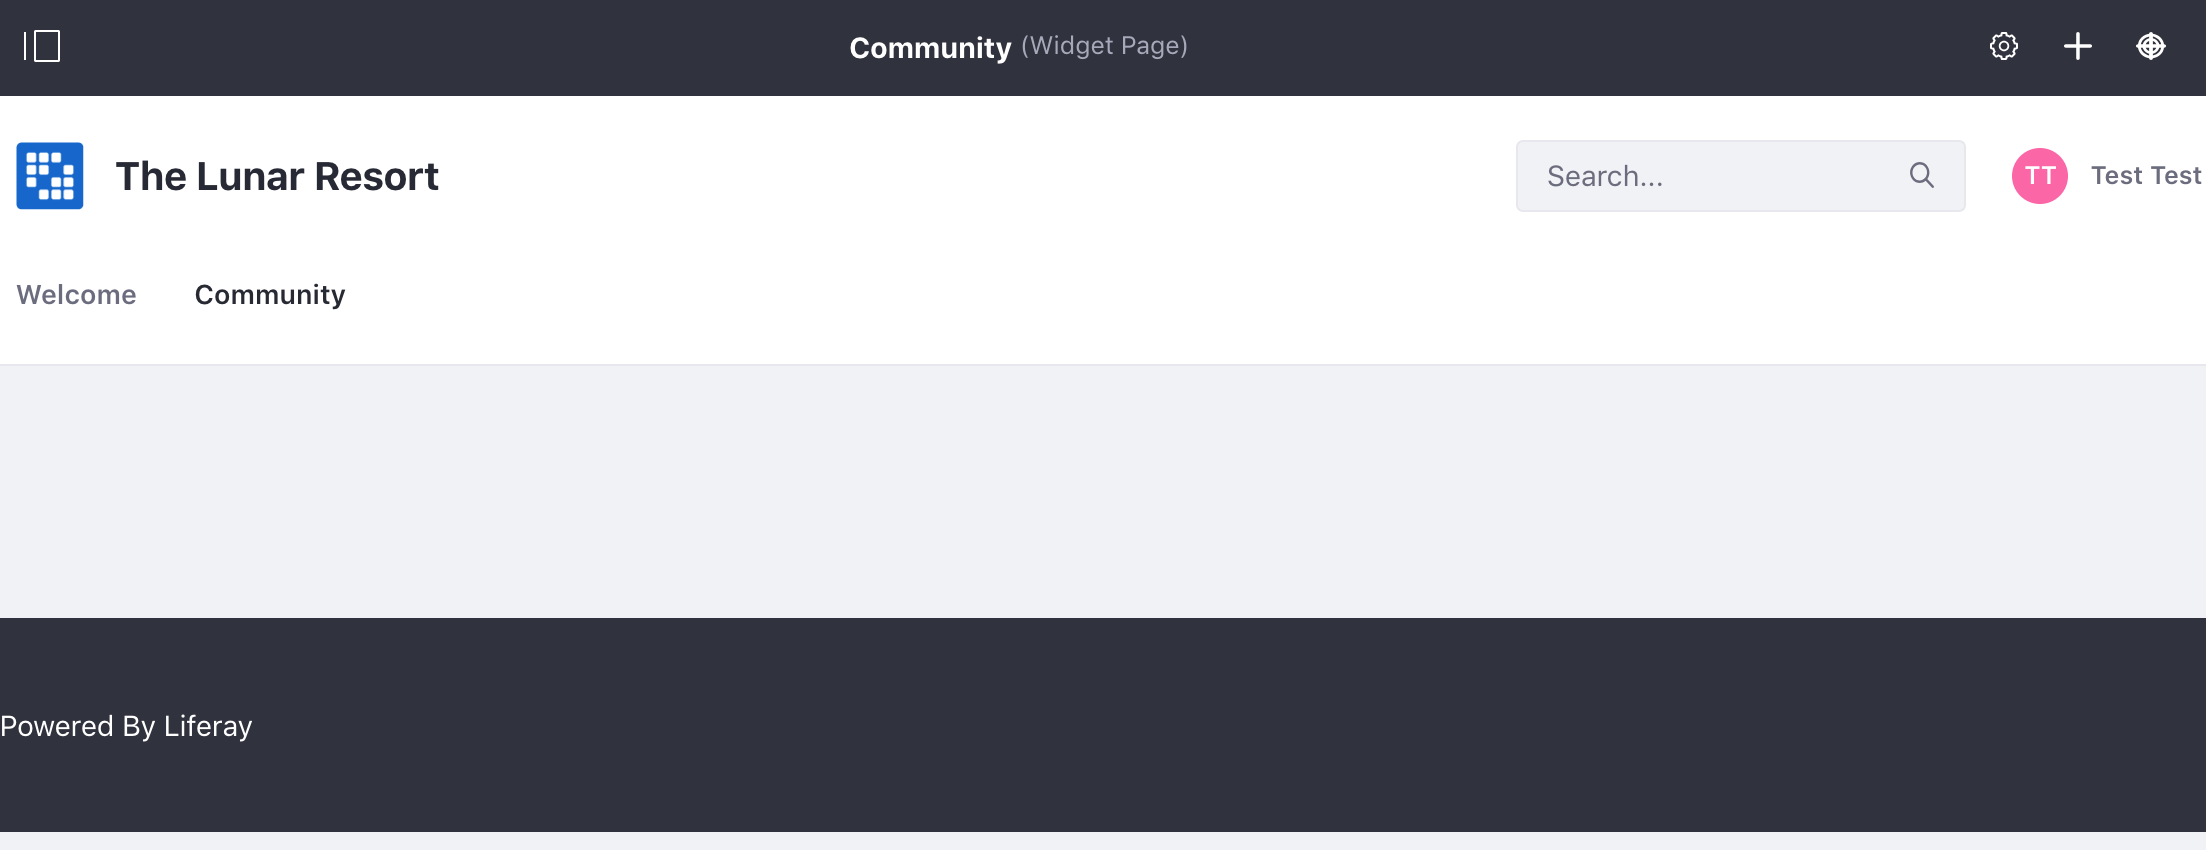
\includegraphics{./images/community-page-created.png}
\caption{Your page has been added to the navigation automatically.}
\end{figure}

\subsection{Adding Widgets to a Page}\label{adding-widgets-to-a-page}

To add widget to a page, go to the page and click the \emph{Add} button
(\includegraphics{./images/icon-control-menu-add.png}) from the top menu
and select the \emph{Widgets} tab. You can either browse through the
categories of available widgets until you find the one you want, or you
can search for widgets by name. Once you've found a widget, click the
\emph{Add} button to add it to the current page. Once there, you can
drag it to a new position. Alternatively, you can drag the widget
directly from the Widgets menu to a specific location on the page.
Follow the steps below to add some Collaboration apps to the Lunar
Resort Site.

\begin{enumerate}
\def\labelenumi{\arabic{enumi}.}
\item
  From the top menu, select \emph{Add} → \emph{Widgets}.
\item
  In the menu that appears, expand the \emph{Collaboration} category.
\item
  Drag the \emph{Blogs Aggregator} widget onto the right column of your
  page.
\item
  Next, drag the \emph{Wiki} app to the left column.
\end{enumerate}

See how easy it is to add applications to your pages? You've added the
Wiki app and Blogs Aggregator app to a page.

\begin{figure}
\centering
\includegraphics{./images/app-layout-design.png}
\caption{Your page layout options are virtually limitless with a slew of
application and layout combinations.}
\end{figure}

If the default layout options provided aren't enough, you can create
your own. For more information about developing custom layout templates,
see the tutorial
\href{/docs/7-1/tutorials/-/knowledge_base/t/creating-layout-templates-with-the-themes-generator}{Layout
Templates with the Liferay Theme Generator}.

\noindent\hrulefill

Note: Portlets are rendered according to
\href{https://docs.liferay.com/ce/portal/7.1-latest/definitions/liferay-portlet-app_7_1_0.dtd.html\#render-weight}{\texttt{render-weight}}
on Widget Pages.

\noindent\hrulefill

Next, you'll look at creating reusable templates for widget pages.

\section{Creating Widget Pages from
Templates}\label{creating-widget-pages-from-templates}

Page templates provide pre-configured pages to reuse. There are two
types of page templates in 7.0: Widget Page templates consist of a
portlet layout and configuration. Content Page templates are constructed
from Fragments. You can read about
\href{/docs/7-1/user/-/knowledge_base/u/building-content-pages-from-fragments}{Content
Page Templates in this article}.

Three sample layout page templates are installed by default:

\begin{itemize}
\item
  \textbf{Search:} Contains a search bar and configuration to display
  various facets.
\item
  \textbf{Wiki:} Provides a page with three applications related to
  authoring a wiki.
\item
  \textbf{Blog:} Provides a page with three applications related to
  blogging.
\end{itemize}

\begin{figure}
\centering
\includegraphics{./images/default-page-templates.png}
\caption{The Blog page template is already available for use along with
the Search and Wiki page templates.}
\end{figure}

To add a new widget page template,

\begin{enumerate}
\def\labelenumi{\arabic{enumi}.}
\item
  Go to \emph{Build} → \emph{Pages}.
\item
  Select the \emph{Page Templates} tab.
\item
  Create a Collection named \emph{Lunar Resort Templates}.
\item
  Click the \emph{Add} icon (\includegraphics{./images/icon-add.png})
  and select *Widget Page Template.
\item
  Enter a \emph{Name}.
\item
  Click \emph{Save}.
\end{enumerate}

The editing page for the template appears. You can add widgets to the
page or access page configuration now. The changes you make are
instantly applied to the template.

If you want to edit the template again,

\begin{enumerate}
\def\labelenumi{\arabic{enumi}.}
\item
  Go back to the \emph{Page Templates} tab.
\item
  Click the \emph{Actions} icon
  (\includegraphics{./images/icon-actions.png}).
\item
  Click \emph{Edit}.
\end{enumerate}

Note that after a new page template has been created, the default
permissions only allow the creator to use the page template. To give
other users access to it,

\begin{enumerate}
\def\labelenumi{\arabic{enumi}.}
\item
  Use the Actions menu for the template and select \emph{Permissions}.
\item
  In the matrix of Roles and permissions, check the \emph{View}
  permission for the Roles needed to see the page template in the list
  of available page templates when creating a new page.
\end{enumerate}

If you want any user who can create a page to be able to use the page
template, check the \emph{View} permission for the \emph{User} Role.

To use your template to create a new page,

\begin{enumerate}
\def\labelenumi{\arabic{enumi}.}
\item
  Go to Site Administration and select the \emph{Pages} option from the
  \emph{Build} menu dropdown option.
\item
  Click the \emph{Add} icon (\includegraphics{./images/icon-add.png}).
\item
  Inside the Lunar Resort collection, select the page template that you
  created.
\item
  Enter the name of your page and click \emph{Submit}.
\end{enumerate}

Pages based on templates can inherit changes from the page template:

\begin{figure}
\centering
\includegraphics{./images/automatic-application-page-template-changes.png}
\caption{You can choose whether or not to inherit changes made to the
page template.}
\end{figure}

By default, when a Site administrator creates pages based on a page
template, future changes to the template are automatically propagated to
those pages. Site administrators can disable this behavior by disabling
the \emph{Inherit Changes} selector. Occasionally, propagation for page
templates fails due to unintended errors. To learn how to manage a
failed page template propagation, visit the
\href{/docs/7-1/user/-/knowledge_base/u/propagating-changes-from-site-templates-to-sites}{Propagating
Changes from Site Templates to Sites} tutorial.

If staging has been enabled, changes to the page template are
automatically propagated to the staged page. These changes must still be
approved before the page is published to live. For this reason, the
automatic propagation of page template changes to the staged page cannot
be turned off and the \emph{Inherit Changes} selector does not appear.

You can read more about staging in the
\href{/docs/7-1/user/-/knowledge_base/u/staging-content-for-publication}{Staging
Content for Publication tutorial}.

\subsection{Sharing Widget Page
Templates}\label{sharing-widget-page-templates}

When importing pages to a new site or environment, you must also import
templates associated with those pages. Generally templates are included
automatically when an associated page is exported, but if not you can
export the template collection separately so the page can be imported to
the new environment. To export page templates,

\begin{enumerate}
\def\labelenumi{\arabic{enumi}.}
\item
  Go to \emph{Site Management} → \emph{Publishing} → \emph{Export}.
\item
  At the top right of the page, click the \emph{Add button}
  (\includegraphics{./images/icon-add.png}) to create a new custom
  export process.
\item
  On the \emph{New Custom Export} page, under the Content section,
  listed under Pages, you can click the \emph{Change} link to choose
  which Collections and templates are being exported.
\item
  When you're done configuring the export, click \emph{Export} and save
  the exported LAR file.
\item
  On the target environment, go to \emph{Site Management} →
  \emph{Publishing} → \emph{Import} and click the \emph{Add button}
  (\includegraphics{./images/icon-add.png}).
\item
  Upload the LAR with your template data. If the LAR contains additional
  content you don't want to import, you can deselect it.
\end{enumerate}

Once the template has been imported, the page can be imported normally
to your new environment. For more information on exporting/importing
content, visit the
\href{/docs/7-1/user/-/knowledge_base/u/importing-exporting-pages-and-content}{Importing/Exporting
Sites and Content} article.

\section{Using Full Page
Applications}\label{using-full-page-applications}

Full Page Applications are the ideal way to display a Message Board,
Wiki, or other application that demands a full page.

\subsection{Configuring the Page}\label{configuring-the-page}

Creating a Full Page Application starts just like creating any other
type of page.

\begin{enumerate}
\def\labelenumi{\arabic{enumi}.}
\item
  Go to \emph{Site Administration} → \emph{Build} → \emph{Site Pages}.
\item
  Click the (\includegraphics{./images/icon-add.png}) icon.
\item
  Give your page a \emph{Name} and click \emph{Submit}.
\end{enumerate}

At this point you created the page, but it contains no content. If you
visit the page, there is no way to add any content or widgets to the
page. You must configure the page for it to function.

\begin{enumerate}
\def\labelenumi{\arabic{enumi}.}
\item
  From \emph{Site Pages} click the
  (\includegraphics{./images/icon-options.png}) button and select
  \emph{Configure}.

  On the next screen, you can change the page's \emph{Name},
  \emph{Friendly URL}, and set the \emph{Full Page Application} as well
  as access other page configuration options in the other tabs.

  \begin{figure}
  \centering
  \includegraphics{./images/full-page-app-configure.png}
  \caption{The Full Page Application configuration page.}
  \end{figure}
\item
  Set the \emph{Full Page Application} to \emph{Wiki} and click
  \emph{Save}.

  Out of the box, you can set the Blogs, Wiki, Media Gallery, Message
  Boards, RSS, Hello Soy Portlet, Documents and Media, or Dynamic Data
  Mapping Form to be the sole application for the page. Developers can
  make their applications Full Page Applications.
\item
  Click \emph{Go to Site} in the Site Administration menu, and then
  click on your page.
\end{enumerate}

Now the page is configured to display the Wiki and only the Wiki. No
other widgets can be added to the page, and the Wiki app cannot be
removed.

\begin{figure}
\centering
\includegraphics{./images/single-page-app-wiki.png}
\caption{The Wiki displayed as a Full Page Application.}
\end{figure}

Note that all of the applications that can be added to the page are
non-instanceable and the content of whichever application you select is
based on the instance for that site. So if you already had data in your
Wiki it appears on this page.

If you want to configure the application to be scoped to this specific
page, you can configure that through the application's settings.

\begin{enumerate}
\def\labelenumi{\arabic{enumi}.}
\item
  From the page, click the (\includegraphics{./images/icon-options.png})
  button for the Wiki and select \emph{Configuration}.
\item
  From the \emph{Wiki - Configuration} page, select the \emph{Scope}
  tab.
\item
  Open the \emph{Scope} menu and select \emph{Space Wiki}.
\end{enumerate}

\begin{figure}
\centering
\includegraphics{./images/configuring-scope.png}
\caption{Configuring the scope.}
\end{figure}

Now the Wiki is scoped for this page, and doesn't share data with the
Site or globally scoped Wiki.

\chapter{Building a Responsive Site}\label{building-a-responsive-site}

Now more than half of all page views in the world come from mobile
devices like phones and tablets. That means that if your pages don't
look good on mobile devices, your pages don't look good for more than
half the people looking at them. Liferay DXP can provide the best
experience possible no matter what device you're using.

Most of the heavy lifting for mobile optimization comes from your
developers. Themes must be designed to be responsive. Web Content
Structures and Templates and Page Fragments must be created with code
that transitions gracefully to fit smaller screens on mobile devices.
But there's work to do for marketers and administrators as well.

\section{Built-in Mobile Support}\label{built-in-mobile-support}

Out of the box, there are several features that help make your pages
look just as good and have the same functionality on mobile devices as
they do on a desktop:

\begin{itemize}
\item
  Liferay Widgets and custom widgets that use Liferay's UI frameworks
  automatically scale to fit the screen size.

  \begin{figure}
  \centering
  \includegraphics{./images/widget-adjustment.png}
  \caption{A widget adjusts its size.}
  \end{figure}
\item
  UI elements like the navigation and Product Menu automatically adjust
  to remain usable on smaller screens.

  \begin{figure}
  \centering
  \includegraphics{./images/navigation-adjustment.png}
  \caption{The main navigation adjusts its size.}
  \end{figure}
\item
  When the screen width is low, Liferay combines columns so that all
  content remains legible.

  \begin{figure}
  \centering
  \includegraphics{./images/columns-adjustment.png}
  \caption{Columns combine.}
  \end{figure}
\item
  For web developers, Liferay's theme tools provide a number of tools to
  help ensure optimum mobile performance.
\end{itemize}

For most business users, this means that all you need to do to display
pages on Mobile device is to create a page. However, you also have tools
available to verify that everything displays as intended. The Device
Simulator (\includegraphics{./images/icon-simulation.png}) is a powerful
tool that shows you how pages look on different devices.

\subsection{Using the Device
Simulator}\label{using-the-device-simulator}

When creating a page or reviewing a page before it is published, one of
your most important tools is the Device Simulator found in the top right
corner of every page. The simulator lets you view the current page in a
number of resolutions based on different display types. There are three
predefined options:

\textbf{Desktop:} Fixes the width to display the page at full size.

\textbf{Tablet:} Puts your page in a box as if it is being displayed on
a tablet. It also activates some of Liferay's built-in mobile features.

\textbf{Mobile:} Puts your page in an even smaller box to demonstrate
how the page looks to your average smartphone user.

\begin{figure}
\centering
\includegraphics{./images/device-simulation.png}
\caption{The Simulation panel defines multiple screen sizes.}
\end{figure}

There are also two options available to display

\textbf{Autosize:} Provides another way to view the default behavior
where the page shrinks and grows based on the width of the browser
window.

\textbf{Custom:} Lets you enter a specific size for testing and fixes
the height and width of the display.

Because modern mobile browsers are built on the same technology as
desktop browsers, the behavior you see in the simulator should match the
experience of users on mobile devices. In addition to making sure the
basic layout looks good and that all functionality remains, it's also
important to make sure that automatic features---like how columns are
combined at lower resolutions---don't have unintended effects.

\subsection{Designing Mobile Friendly
Pages}\label{designing-mobile-friendly-pages}

Liferay DXP provides the tools you need, but building pages that provide
a good experience across all kinds of devices still means working across
all levels of web development and publishing. Theme developers must
create themes that use Liferay's frameworks to scale content well across
all kinds of displays. Designers must have multiple screen sizes in mind
when designing pages. And before anything it published it must be
thoroughly reviewed to make sure that it provides the best experience to
all of your users.

Now that you've learned about Liferay's tools for making your website
mobile friendly, let's look at your options for adapting to different
types of mobile devices.

\chapter{Mobile Device Rules}\label{mobile-device-rules}

With mobile device rules, you can alter what gets displayed based on the
device being used to access Liferay DXP. For instance, you can configure
the look and feel of pages accessed by smartphone or tablet users
differently from those accessed by users on a computer.

Whole Sites or individual pages can be configured for mobile device
families. A family describes a group of devices. You can set rules that
describe a category of devices, such as all Android devices or all iOS
tablets. You can define as many rules in a family as you need to
classify all the devices for which you'd like to define actions.
Families can be prioritized to determine which one applies to a given
page request.

\section{Creating Mobile Device
Rules}\label{creating-mobile-device-rules}

To configure mobile device rules, you need a way to find out the
characteristics of the device. While some of the characteristics are
provided by the device, most are not. For this reason, there are
databases that contain information about thousands of devices. These
databases make it possible to learn every detail about a device from the
device type. Liferay DXP's Mobile Device Rules can connect to device
databases so that you can use their device characteristics in your
rules.

\noindent\hrulefill

\textbf{Important:} For the features described in this article to work,
you must install the Liferay Mobile Device Detection (LMDD) app from
Liferay Marketplace. This app provides the device detection database
that's required to detect which mobile devices are accessing it. Note
that if you're running Liferay DXP, you must install
\href{https://web.liferay.com/marketplace/-/mp/application/92831494}{the
lite version of LMDD} before you can install
\href{https://web.liferay.com/marketplace/-/mp/application/35419014}{the
enterprise version}.
\href{/docs/7-1/user/-/knowledge_base/u/using-the-liferay-marketplace}{Click
here} for instructions on using Liferay Marketplace to find and install
apps.

\noindent\hrulefill

You can develop plugins that integrate with other device databases. Even
if you don't have a device database, you can still set up mobile device
rules. They won't, however, be effective until a database is deployed,
because the portal won't have enough information about the devices being
used to make page requests.

To access the Mobile Device Families administrative page,

\begin{enumerate}
\def\labelenumi{\arabic{enumi}.}
\item
  Open the \emph{Product Menu}.
\item
  Use the \emph{Site Selector}
  (\includegraphics{./images/icon-compass.png}) to choose the Site that
  you want to define Mobile Device Rules for.
\item
  Select \emph{Configuration} → \emph{Mobile Device Families}.
\end{enumerate}

You can also add families for all Sites by navigating to the Control
Panel → \emph{Sites} → \emph{Global}. The Mobile Device Families
administrative page displays a list of defined families and lets you add
more. To add rules, you must first add a family.

\begin{enumerate}
\def\labelenumi{\arabic{enumi}.}
\item
  Click \emph{Add} button (\includegraphics{./images/icon-add.png}) to
  add a \emph{New Device Family}.
\item
  Enter a \emph{Name} and \emph{Description}.
\item
  Click \emph{Save}.
\item
  Click on the name of the Mobile Device Family to access the rules
  page.
\end{enumerate}

\begin{figure}
\centering
\includegraphics{./images/mobile-device-families.png}
\caption{Create a Mobile Device Family so you can create rules.}
\end{figure}

The rules defined for a family, along with the priorities of the
families selected for a particular Site or page, determine which
family's actions are applied to a given request. From the New
Classification Rule page for a specific rule set, you can add a rule by
specifying an operating system, rule type, physical screen size, and
screen resolution. Remember that you can add as many rules to a family
as you need in order to classify the devices on which you'd like to take
actions.

\begin{enumerate}
\def\labelenumi{\arabic{enumi}.}
\item
  Click on the \emph{Add} button
  (\includegraphics{./images/icon-add.png}) to add a new rule.
\item
  Enter a \emph{Name} and \emph{Description}.
\item
  Select the classifications you want for this rule from \emph{Operating
  System and Type}, \emph{Physical Screen Size}, and \emph{Screen
  Resolution}.
\item
  Click \emph{Save}.
\end{enumerate}

You'll notice after saving the classification rule that it's
characterized as a \emph{Simple Rule}. Only Simple Rules are included
with Liferay DXP, but the rules are designed to be extensible, and
additional rule types can be added by your developers.

\begin{figure}
\centering
\includegraphics{./images/mobile-device-editing-rule.png}
\caption{Select the operating system and device type for your rule.}
\end{figure}

Once you've created some mobile device families and added some rules to
them, you're ready to create some actions. The actions defined for a
family determine what happens to a request when the device is detected
and the family has been found to apply.

\noindent\hrulefill

\textbf{Tip:} The Audience Targeting application offers a \emph{Device}
rule that evaluates whether a User is accessing content using a
particular device family. This rule is integrated with the Mobile Device
Families app.

\noindent\hrulefill

You can add families to a Site, individual page, or page set from their
respective configuration pages. To do it for a Page Set:

\begin{enumerate}
\def\labelenumi{\arabic{enumi}.}
\item
  Go to \emph{Build} → \emph{Pages} in your Site.
\item
  Click on \emph{Configuration}
  (\includegraphics{./images/icon-page-gear.png}) for the Public Pages.
\item
  Select the \emph{Advanced} tab and open the \emph{Mobile Device Rules}
  option in the bottom menu.
\item
  Click \emph{Select} to open the list of families that can be applied.
\end{enumerate}

From the same page, you can access the configuration for an individual
page, or you can configure Mobile Device Rules for an entire Site from
\emph{Configuration} → \emph{Site Settings}. You can select multiple
families for a particular Site or page and order them by priority. The
families are checked in decreasing order of priority: the actions
defined by the first family that applies are executed.

\begin{figure}
\centering
\includegraphics{./images/mobile-device-selection.png}
\caption{You can select a mobile device family to apply for a Site or
page.}
\end{figure}

\section{Mobile Device Actions}\label{mobile-device-actions}

After you've created families and applied rules to define those
families, you can associate specific actions that occur when a user
visits that Site on a device.

To add actions to a selected rule group:

\begin{enumerate}
\def\labelenumi{\arabic{enumi}.}
\item
  Go to the \emph{Configuration} page for the page, page set, or Site
  where you have configured a device family.
\item
  In the \emph{Mobile Device Rules} section, click \emph{Actions}
  (\includegraphics{./images/icon-actions.png}) → \emph{Manage Actions}
  next to the device family that you wish to add an action for.
\item
  Click \emph{Add Action}.
\end{enumerate}

\begin{figure}
\centering
\includegraphics{./images/manage-mobile-actions.png}
\caption{Getting to the Manage Actions page.}
\end{figure}

By default, there are four kinds of actions that can be configured for
mobile families:

\textbf{Layout Template Modification:} Changes the way portlets are
arranged on pages delivered to mobile devices. For example, you could
have pages with more complex layouts automatically switch to a simpler
template if it detects a mobile device---even if the resolution is
theoretically high enough to support the standard layout.

\textbf{Theme Modification:} Selects a specific theme for different
mobile device families. You'd have to have a mobile version of your
Site's theme that is automatically applied when a device hits your page.

\textbf{URL Redirect:} Sends mobile users to any URL. This can be used
to direct mobile users to a mobile app download or a mobile version of
the page.

\textbf{Site Redirect:} Sends mobile users to a different Site on your
portal. In some cases, mobile content could be created on a mirror of
your Site.

\noindent\hrulefill

\textbf{Tip:} 7.0 was designed from the ground up to be responsive and
adapt to any device that might be accessing it. Before creating new
themes or forcing a layout template change, you should test how the Site
behaves using Liferay DXP out of the box. Certain features, like URL
Redirects, can be disruptive and frustrating for users if used
improperly.

\noindent\hrulefill

Like mobile device rules, mobile device actions are extensible. Your
developers can define custom actions in addition to the four actions
provided by default.

To review, if you want to configure an action or actions that take place
when mobile device requests are received, take the following steps:

\begin{enumerate}
\def\labelenumi{\arabic{enumi}.}
\item
  Create a mobile device family to represent the group of devices for
  which to define an action or actions.
\item
  Define one or more rules for your family that describe the group of
  devices represented by your family.
\item
  Apply your family to an entire page set of a Site (all the public
  pages of a Site or all the private pages) or to a single page.
\item
  Define one or more actions for your family that describe how requests
  should be handled.
\end{enumerate}

\subsection{Mobile Device Rules
Example}\label{mobile-device-rules-example}

Now you'll look at an example of using mobile device rules. Suppose you
want to create a rule so that when a Site is accessed by an Android or
iOS tablet, a different layout is used. To set this up, you must follow
the same four steps described above.

First create the Mobile Device Family:

\begin{enumerate}
\def\labelenumi{\arabic{enumi}.}
\item
  Navigate to the \emph{Mobile Device Families} page of \emph{Site
  Administration}.
\item
  Click \emph{Add Device Family}
  (\includegraphics{./images/icon-add.png}).
\item
  Enter \emph{Android and iOS Tablets} for the \emph{Name}.
\item
  Click \emph{Save}.
\end{enumerate}

Next create a rule for the family:

\begin{enumerate}
\def\labelenumi{\arabic{enumi}.}
\item
  From the \emph{Mobile Device Families} page, click on \emph{Android
  and iOS Tablets}.
\item
  Click \emph{Add Classification Rule}
  (\includegraphics{./images/icon-add.png}).
\item
  Name the rule \emph{Rule 1}.
\item
  Under \emph{Operating System} select \emph{Android} and \emph{iPhone
  OS} (you can hold or to select multiple items).
\item
  Under \emph{Device Type} select \emph{Tablets},
\item
  Click \emph{Save}.

  \begin{figure}
  \centering
  \includegraphics{./images/example-classification-rule.png}
  \caption{Create the Classification rule.}
  \end{figure}
\end{enumerate}

As with the previous example, you only need one rule to describe your
device family. Now you must apply the rule to some pages.

\begin{enumerate}
\def\labelenumi{\arabic{enumi}.}
\item
  Go to \emph{Build} → \emph{Pages} in Site Administration.
\item
  Click on the \emph{Configuration} icon for the \emph{Public Pages}
\item
  Go to the \emph{Advanced} tab.
\item
  Under \emph{Mobile Device Rules}, select the \emph{Android and iOS
  Tablets} device family.
\end{enumerate}

Now you must define an action for your Android and iOS Tablets rule
group to use a different layout.

\begin{enumerate}
\def\labelenumi{\arabic{enumi}.}
\item
  Click \emph{Actions} → \emph{Manage Actions} for the \emph{Android and
  iOS Tablets} rule.
\item
  Click \emph{Add Action}.
\item
  Enter the name \emph{Layout Template Modification}, and select the
  \emph{Layout Template Modification} action type.
\item
  Select the \emph{1 Column} layout template.
\item
  Click \emph{Save}.
\end{enumerate}

\begin{figure}
\centering
\includegraphics{./images/example-mobile-action.png}
\caption{Create the Actions for Android and iOS Tablets.}
\end{figure}

Now the Liferay Site's pages are presented to Android and iOS tablet
users with the 1 Column layout template.

Mobile Device Rules are a powerful way to manage the way pages and
content appear on the various devices that access your Site. But
remember to consider the power of modern devices and the experience of
your users, and use this great power responsibly---to help users have a
great experience on your website and to not interrupt or negatively
impact that experience on whatever device they're using.

\chapter{Managing Site Navigation}\label{managing-site-navigation}

Liferay provides powerful tools for creating and organizing pages. You
can have anything from a simple, flat Site navigation to a complex
hierarchy with tree of sub-pages nested down many levels.

7.0 lets you create Navigation Menus separate from your page hierarchy.
Now you have the freedom to leave one-off marketing landing pages out of
the navigation or create multiple navigation menus: a main menu,
secondary menus, footer menus, and custom menus for anything that you
can dream up.

Menus can differ by page: landing pages can show a simple list of
frequently visited pages, and the rest can appear in secondary
navigation. You can also create specific menus for different landing
pages to direct users to content that is relevant to them.

Go to \emph{Navigation} → \emph{Pages} to view the existing pages or
create new pages. The Site hierarchy as displayed on \emph{Pages} is the
main reference for the organization of pages on that Site. While
Navigation Menus can customize their organization and what appears and
what doesn't appear, this menu is always the primary reference for the
pages on your Site.

\section{Page Hierarchy}\label{page-hierarchy}

Using the Page Hierarchy, you create public and private pages and
organize those pages in whatever order or structure that you see fit.

\subsection{Creating a Page}\label{creating-a-page}

New pages are created on the \emph{Build} → \emph{Pages} page in Site
Administration. Pages can be created as \emph{Public Pages} which anyone
can view, or \emph{Private Pages} which can only be viewed by Site
Members. To create a new page,

\begin{enumerate}
\def\labelenumi{\arabic{enumi}.}
\tightlist
\item
  Go to \emph{Site Administration} for the Site you want to work on,
  then \emph{Build} → \emph{Pages}.
\end{enumerate}

\begin{figure}
\centering
\includegraphics{./images/default-nav-pages.png}
\caption{In the default site, initially only the \emph{Welcome} and the
hidden \emph{Search} pages exist in the Public Pages Hierarchy.}
\end{figure}

\begin{enumerate}
\def\labelenumi{\arabic{enumi}.}
\setcounter{enumi}{1}
\item
  Click \emph{Add} \href{./images/icon-add.png}{Add Page} and select
  \emph{Public Page}.
\item
  Select \emph{Widget Page}.
\item
  Set the \emph{Name} as \emph{About Us}.
\item
  Click \emph{Save}.
\item
  On the next page, note the \emph{Show in Public Page Hierarchy Menu}
  selection, leave the defaults and click \emph{Save}.
\end{enumerate}

\begin{figure}
\centering
\includegraphics{./images/page-hierarchy-menu.png}
\caption{When you create a page, by default it is added to the site
hierarchy.}
\end{figure}

Now that the page is created, it appears in the hierarchy, and you can
move or organize its position there.

\subsection{Organizing Pages}\label{organizing-pages}

Drag and drop pages to reorder their position in the page hierarchy (and
subsequently the default navigation that users see), and to nest them as
subpages. The page at the top of the list is the \emph{Home} page that
users see automatically when visiting your Site.

\begin{enumerate}
\def\labelenumi{\arabic{enumi}.}
\tightlist
\item
  Click \emph{Go to Site} to view the organization of the navigation
  menu. You can see the order of the pages matches the order of the
  pages from Site Administration.
\end{enumerate}

\begin{figure}
\centering
\includegraphics{./images/navigation-practical1.png}
\caption{You can see the order of pages in Site Administration vs.~how
they appear on the site.}
\end{figure}

\begin{enumerate}
\def\labelenumi{\arabic{enumi}.}
\setcounter{enumi}{1}
\item
  Drag the \emph{About Us} page above the \emph{Welcome} page in the
  list. It automatically becomes the \emph{Home} page.
\item
  Click \emph{Go to Site} to see how this affects your menu.
\end{enumerate}

\begin{figure}
\centering
\includegraphics{./images/navigation-practical2.png}
\caption{\emph{About Us} is now the home page, and \emph{Welcome} is
second in the nav.}
\end{figure}

\begin{enumerate}
\def\labelenumi{\arabic{enumi}.}
\setcounter{enumi}{3}
\item
  Drag \emph{About Us} on top of \emph{Welcome} to nest it.
\item
  Click \emph{Go to Site} one more time to see how nested pages appear.
\end{enumerate}

\begin{figure}
\centering
\includegraphics{./images/navigation-practical3.png}
\caption{\emph{About Us} is now nested under \emph{Welcome} and appear
when you mouse-over \emph{Welcome}.}
\end{figure}

As you've just demonstrated, organizing pages in the default menu is
simple, but very powerful.

\subsubsection{Public and Private Pages}\label{public-and-private-pages}

As noted above, Private Pages work just like Public Pages, except they
can be viewed only by registered members of a Site. In the default
configuration, Public Pages are at the URL
\texttt{{[}web-address{]}/}\textbf{web}\texttt{/{[}site-name{]}} while
Private Pages are at
\texttt{{[}web-address{]}/}\textbf{group}\texttt{/{[}site-name{]}}.
Other than the membership distinctions, Public and Private Pages share
the same behavior.

\subsection{Page Options}\label{page-options}

While managing the default menu, you can also access page options.
Clicking on the \emph{Options} icon
\href{./images/icon-options.png}{Option} accesses several configuration
tools:

\begin{itemize}
\item
  \textbf{View} goes to the selected page on the Site.
\item
  \textbf{Configure} goes to page configuration.
\item
  \textbf{Copy Page} creates a new page in the current Site that
  duplicates the selected page.
\item
  \textbf{Permissions} opens the Permissions dialog.
\item
  \textbf{Orphan Widgets} clears data related to widgets that have been
  removed from the page.
\item
  \textbf{Delete} deletes the page and all its data.
\end{itemize}

Creating and managing pages using the page hierarchy is simple but very
powerful. If you need more navigation options, however, Navigation Menus
provide more flexibility.

\section{Creating and Managing Navigation
Menus}\label{creating-and-managing-navigation-menus}

To better understand Navigation Menus, it's time to create a new menu.

\subsection{Creating a Navigation
Menu}\label{creating-a-navigation-menu}

\begin{enumerate}
\def\labelenumi{\arabic{enumi}.}
\item
  Go to \emph{Site Administration} → \emph{Build} → \emph{Navigation
  Menus}.
\item
  Click the \texttt{+} button to add a new menu.
\item
  Give your menu a name and click \emph{Submit}.
\end{enumerate}

On the next page appears a number of elements that you can add to a
menu.

\textbf{Page}: Select an existing page from the current Site to add to
the navigation menu.

\textbf{Submenu}: Create a second level of menu navigation.

\textbf{URL}: Create a link to any page anywhere by providing a URL. The
link appears just like any other option in your menu.

Click on \emph{Page} and you see a view of all the current pages on the
current Site. Select a page and click \emph{Add} to add that page to the
menu.

\noindent\hrulefill

\textbf{Note:} When you click on a page, you select that page. Multiple
pages can be selected by clicking on each page one at a time. To
deselect a page, click on the page again.

\noindent\hrulefill

Now you see the menu management screen. From here, you can drag and drop
menu elements to rearrange or nest them. You can also manage options for
this menu by clicking the gear icon in the top right. Let's add another
item to the menu.

\begin{enumerate}
\def\labelenumi{\arabic{enumi}.}
\item
  Click the \texttt{+} icon.
\item
  Select \emph{Submenu} in the menu that pops up.
\item
  Name your menu \emph{External Links}.
\item
  Click \emph{Add}.
\end{enumerate}

Click the \texttt{+} button again and select \emph{URL}. You're prompted
to enter a page name and URL.

\begin{enumerate}
\def\labelenumi{\arabic{enumi}.}
\item
  Enter a \emph{Name}.
\item
  Enter the \emph{URL} for an external Site.
\item
  Click \emph{Add}.
\end{enumerate}

Drag the URL item onto the \emph{External Links} submenu. This nests the
URL item in the submenu.

\begin{figure}
\centering
\includegraphics{./images/basic-nav-menu.png}
\caption{Menus can have a standard page, a submenu, and a URL link in
the submenu.}
\end{figure}

Now that you can see how menus work, you can learn the details.

\subsection{Managing Menus}\label{managing-menus}

After you create a menu, more configuration options appear on the main
Navigation Menus page.

\textbf{Title}: Your menu's name.

\textbf{Add New Pages}: Determines if new pages added to the main
navigation are added to the menu automatically.

\textbf{Marked As}: Can be set as \emph{Primary Navigation},
\emph{Secondary Navigation}, or \emph{Social Navigation}.

\textbf{Author}: The user that created the menu.

\textbf{Create Date}: When the menu was created.

Theme and Fragment developers primarily use the menu types to determine
how a menu should be styled. \textbf{Primary Navigation} is the main
navigation for a page. \textbf{Secondary Navigation} is a second level
of navigation, possibly a sidebar or a separate menu within a page.
\textbf{Social Navigation} is for menus that contain links for sharing
content on social media or similar tasks.

\subsubsection{Modifying Menus}\label{modifying-menus}

Next click on the options menu at the far left of your new navigation
menu:

\begin{figure}
\centering
\includegraphics{./images/nav-menu-options.png}
\caption{Menus with a standard page, a submenu, and a URL link in the
submenu are created for different reasons.}
\end{figure}

\textbf{Edit}: Add, remove, or organize menu items.

\textbf{Rename}: Change the name of your menu.

\textbf{Permissions}: Define who can view, update, delete, and manage
the permissions for the menu.

\textbf{Mark As}: Change the menu type.

\textbf{Delete}: Deletes the menu.

Next you'll learn about the tools for displaying menus on pages.

\section{Displaying Navigation Menus}\label{displaying-navigation-menus}

You can display Navigation Menus in different ways on your Site. You may
want to configure different display styles for a main menu, sidebar, and
footer menu all on one page.

\subsection{The Navigation Menu
Widget}\label{the-navigation-menu-widget}

The Navigation Menu widget lets you add navigation wherever you need it.
You can place the widget on a page and then select a menu and style for
the menu you are displaying.

\begin{enumerate}
\def\labelenumi{\arabic{enumi}.}
\item
  Go to a Widget Page, open the Add menu on the right side of the page
  and add the \emph{Content Management} → \emph{Navigation Menu} to the
  page.
\item
  Open the \emph{Configuration} menu.
\end{enumerate}

From here you can configure three main categories:

\begin{itemize}
\item
  The Navigation Menu to be displayed
\item
  The styling of the menu
\item
  What level of navigation to display
\end{itemize}

\begin{figure}
\centering
\includegraphics{./images/nav-widget-configuration.png}
\caption{Configuring the Navigation Menu Widget.}
\end{figure}

\subsubsection{Choosing a Navigation
Menu}\label{choosing-a-navigation-menu}

The Navigation Menu Widget has two ways to select a menu. You can choose
to \emph{Select Navigation} or \emph{Choose Menu}.

\textbf{Select Navigation:} Select from the three main menu types:
\emph{Primary Navigation}, \emph{Secondary Navigation}, and \emph{Social
Navigation}.

\textbf{Choose Menu:} Choose any menu that was created for that Site.

Once you select a menu, you must choose how to display it.

\subsubsection{Display Template}\label{display-template}

The \emph{Display Template} option lets you select an
\href{/docs/7-0/user/-/knowledge_base/u/application-display-templates}{Application
Display Template} for Navigation Menus. There ten included by default:

\textbf{List Menu:} Displays all the items in a vertical list.

\textbf{Pills Horizontal:} Displays the items horizontally and uses a
button style for highlighting.

\textbf{Pills Justified:} Like Pills Horizontal, but pads the items to
fill out the horizontal space.

\textbf{Pills Stacked:} A vertical version of the pills style.

\textbf{Tabs:} Displays the items like navigation tabs.

\textbf{Tabs Justified:} Navigation tabs that fill horizontal space.

\textbf{Bar Minimally Styled:} A lightweight version of the default
display that you see in the embedded menu on your page.

\textbf{Bar Minimally Justified Styled:} Like Bar Minimally Styled with
horizontal padding.

\textbf{Bar Default Styled:} The default embedded menu.

\textbf{Split Button Dropdowns:} Displays each item as a button with a
dropdown for multiple navigation levels.

You can also add your own
\href{/docs/7-0/tutorials/-/knowledge_base/t/application-display-templates}{custom
templates}.

\subsubsection{Menu Items to Show}\label{menu-items-to-show}

\emph{Menu Items to Show} configures which pages at what level from the
menu are displayed in the widget. You can choose the starting level, how
many levels deep to display, and how to display sub-levels.

\textbf{Start with Menu Items In:} Choose to start at a specific level
of the navigation or a level relative to the current level (above or
below).

\textbf{Sublevels to Display:} Select the number of levels to display in
the navigation, from \textbf{1} down to \textbf{Infinite}.

\textbf{Expand Sublevels:} Choose if hovering your mouse over the
navigation reveals navigation levels one at a time automatically or
reveal all the levels at once.

Now you can see how there are a variety of customizations and
configurations available for navigation menus that you can implement for
your Site.

\begin{figure}
\centering
\includegraphics{./images/navigation-menu-examples.png}
\caption{Navigation menus give you many ways to help users navigate your
Site.}
\end{figure}

\chapter{Building Sites from
Templates}\label{building-sites-from-templates}

Site Templates create a single Site structure that can be used for any
new Site. They are created and administered from the Control Panel. In
addition to creating multiple Sites with the same design, you can also
use them to manage changes across multiple Sites with propagation of
changes. Site templates can contain multiple pages, each with its own
theme, layout template, applications, and app configurations.

Site templates can also contain content just like actual Sites. This
allows administrators to use Site Templates to create new Sites that are
each created with the same default pages, applications, and content.
After they've been created, these Sites and their pages can be modified
by Site administrators. Using Site templates can save Site
administrators a lot of work even if each Site that was created from a
given Site Template ends up being very different.

\section{Creating a Site Template}\label{creating-a-site-template}

Suppose you need to create the following three private Sites for the
Lunar Resort's internal use: Engineering, Marketing, and Legal. These
should be accessible only to members of these respective departments.
You could design each Site separately, but you can save yourself time if
you create a Site template instead.

\begin{enumerate}
\def\labelenumi{\arabic{enumi}.}
\item
  Go to the Control Panel and click \emph{Sites} → \emph{Site
  Templates}.
\item
  Click the \emph{Add} icon (\includegraphics{./images/icon-add.png})
  and enter the name \emph{Department} for your template.
\item
  Leave the \emph{Active} and \emph{Allow Site administrators to modify
  pages associated with this Site template\ldots{}} boxes checked.
\item
  Click \emph{Save} to create your Site template.
\end{enumerate}

The \emph{Active} box must be checked for your template to be usable. If
your template is still a work in progress, uncheck it to ensure that no
one uses it until it's ready. Checking \emph{Allow Site administrators
to modify pages associated with this Site template\ldots{}} allows Site
administrators to modify or remove the pages and apps that the template
introduces to their Sites---if you want the templates to be completely
static, you should uncheck this.

Now it's time to edit your Site template. This example, includes four
pages.

\noindent\hrulefill

This section assumes knowledge of Liferay 7.1 page management. For more
information on how to create and manage pages in Liferay 7.1, see the
\href{/docs/7-1/user/-/knowledge_base/u/creating-and-managing-pages}{Adding
Pages to Sites tutorial}.

\noindent\hrulefill

\begin{enumerate}
\def\labelenumi{\arabic{enumi}.}
\item
  Click the \emph{Options} icon
  (\includegraphics{./images/icon-options.png}) and select
  \emph{Manage}.

  This brings you to the \emph{Pages} page for the Site Template. You
  already have a home page. Create three more pages.
\item
  Create a \emph{Full Page Application} page named \emph{Documents}.
\item
  Click \emph{Options} (\includegraphics{./images/icon-actions.png}) →
  \emph{Configure} and set the \emph{Full Page Application} to
  \emph{Documents and Media}.
\item
  Create a page using the Global Page Template \emph{Wiki} and name it
  \emph{Wiki}.
\item
  Create a widget page named \emph{Message Boards}.
\item
  Click \emph{Go to Site} in the menu to the left to go to the pages you
  just created.
\item
  On the \emph{Home} page add the Activities, Announcements, and
  Calendar apps.
\item
  On the \emph{Message Boards} page add the Message Boards and Tag Cloud
  apps.
\end{enumerate}

The changes you made to your Site template above are completed in real
time, so there's no \emph{Save} button.

\begin{figure}
\centering
\includegraphics{./images/editing-site-template.png}
\caption{You can see the name of the Site template you're currently
editing.}
\end{figure}

Next, you'll use your Site template to create the Engineering, Marketing
and Legal Sites.

\begin{enumerate}
\def\labelenumi{\arabic{enumi}.}
\item
  Go to the Control Panel and click on \emph{Sites} → \emph{Sites}.
\item
  Click the \emph{Add} icon (\includegraphics{./images/icon-add.png}) →
  \emph{Department}.
\item
  Enter \emph{Engineering} for the Site name.
\item
  Check the \emph{Create default pages as private (available only to
  members). If unchecked, they will be public (available to anyone)}
  option since the Engineering Site is intended for internal use only.
\item
  Click \emph{Save}.
\item
  In the next section, set the Membership Type to \emph{Private}.

  Recall that private Sites don't appear in the My Sites application so
  that regular users won't even know that the Engineering Site exists.
  Also, the only way users can be added to a private Site is via an
  invitation from a Site administrator.
\item
  Leave the \emph{Active} selector enabled so that your Site can be used
  immediately.
\item
  Check the \emph{Create default pages as private (available only to
  members). If unchecked, they will be public (available to anyone).}
  option since the Engineering Site is intended for internal use only.
\item
  Leave the \emph{Enable propagation of changes from the Site template}
  box enabled so that the Engineering Site receives updates if the
  Department Site template is modified.
\item
  Click \emph{Save} to create your Engineering Site.
\item
  Repeat these steps to create the Marketing and Legal Sites.
\end{enumerate}

The new Sites have all the pages and apps you created in the Site
template. To view the pages of the new Sites, click \emph{Sites} →
\emph{Sites} in the Control Panel and then click \emph{Actions} →
\emph{Go to Private Pages} next to one of your new Sites.

Using Site templates streamlines the Site creation process for
administrators, making it easy to create Sites quickly. Now each
department of the Lunar Resort has its own Calendar, Documents and Media
Library, Wiki, and Message Boards on their Sites. Although the pages and
apps of each department's Site are the same, each Site will quickly be
filled with department-specific information as users add and share
content within the Sites. Also, Site administrators can add new pages,
apps, and content to their Sites, further differentiating each
department's Site from the others.

\section{Managing Site Templates}\label{managing-site-templates}

To get started, click on \emph{Site Templates} in the Sites section of
the Control Panel. Here, you can add, manage, or delete Site templates.
You can also configure the permissions of Site templates. As long as a
Site is linked to the Site template it was created from, changes to the
Site template's pages, apps, and app configurations are propagated to
the Site. Changes to a Site template's content, however, are not
propagated to existing Sites that are linked to the Site template.
You'll learn about the propagation of changes between Site templates and
Sites in more detail in the section on Site template use cases below.

To manage a Site Template's pages,

\begin{enumerate}
\def\labelenumi{\arabic{enumi}.}
\item
  Click on \emph{Site Templates} in the Control Panel.
\item
  Select the \emph{Actions} icon
  (\includegraphics{./images/icon-actions.png}) and then \emph{Manage}
  for an existing template.
\end{enumerate}

If you open the main Menu on the left side of your screen (if
necessary), the Site Template is selected in the Site Administration
dropdown menu. You're provided similar options as a regular Site,
including \emph{Build}, \emph{Content}, \emph{Configuration}, and
\emph{Publishing}. By default, the Manage Interface opens \emph{Build} →
\emph{Pages}. From here, you can add or remove pages from a Site
Template or select themes and layout templates to apply to the Site
Template. You can also configure each page to have any theme, any layout
template, and any number of applications, just like a page of a regular
Site. As with Site pages, you can organize a Site Template's pages into
hierarchies. When you create a Site using a Site template, the
configuration of pages and apps is copied from the template to the Site.
By default, all changes made to the Site template are automatically
copied to Sites based on that template.

\noindent\hrulefill

\textbf{Tip:} If you want to publish a piece of web content to many
Sites and ensure modifications are applied to all, don't use Site
template content for that purpose. Instead, place the content in the
global scope and then reference it from a \emph{Web Content Display}
application in each Site.

\noindent\hrulefill

The Content section offers separate repositories for content related
apps based on your Site Template. For instance, by clicking \emph{Polls}
from the Content section, you can create a poll question that is only
available for that specific Site template. Assets created within your
template's Content section can only be accessed by Sites using the
template.

The Configuration section includes Application Display Templates and
Mobile Device configuration options for your Site Template. Also, nested
in the Configuration section is the \emph{Site Template Settings}. This
edits the template's name and description while also offering boolean
options for activating your Site template and allowing Site
administrators to modify pages associated with your template.

The following figure displays the form shown when editing the
\emph{Department} template's settings:

\begin{figure}
\centering
\includegraphics{./images/site-template-settings.png}
\caption{Site templates have several configurable options including the
option to allow Site administrators to modify pages associated with the
Site template.}
\end{figure}

By default, the following Site templates are provided:

\begin{itemize}
\item
  \textbf{Intranet Site:} Provides a preconfigured Site for an intranet.
  The Home page displays the activities of the members of the Site,
  search, a language selector, and a list of the recent content created
  in the intranet. It also provides two additional pages for Documents
  and Media and external News obtained through public feeds.
\item
  \textbf{Community Site:} Provides a preconfigured Site for building
  online communities. The Home page of a \emph{community Site} provides
  message boards, search, a display of a poll and statistics of the
  activity of community members. The Site will also be created with a
  page for a wiki.
\end{itemize}

Now that you know the basics for creating and managing your Site
templates, you can learn about propagating changes next.

\section{Propagating Changes from Site Templates to
Sites}\label{propagating-changes-from-site-templates-to-sites}

Site Template administrators can add, update, or delete Site Template
pages. Changes made to a Site Template can be propagated to Sites whose
page sets are linked to the Site Template. When you create a Site based
on a Site Template with the \emph{Enable propagation of changes from the
Site template} box checked this link is created. To configure
propagation of changes:

\begin{enumerate}
\def\labelenumi{\arabic{enumi}.}
\item
  Select the Site from the Sites dropdown in the Menu by selecting the
  \emph{Site Selector} button
  (\includegraphics{./images/icon-compass.png}).
\item
  Navigate to the \emph{Configuration} → \emph{Site Settings} page and
  uncheck or recheck the \emph{Enable propagation of changes from the
  Site template} checkbox.
\end{enumerate}

In this section, you'll learn about the propagation of changes from Site
templates to Sites and discuss the options available to Site
administrators and Site template administrators.

\subsection{Site Template Page
Behavior}\label{site-template-page-behavior}

If a Site's page set has been created from a Site template and the
propagation of changes from the Site template is enabled, Site
administrators can add new pages but cannot remove or reorder the pages
imported from the Site Template. If a Site has both pages imported from
a Site template and custom Site pages, the Site Template pages always
appear first in the Site page hierarchy; custom pages added by Site
administrators appear after the Site template pages. Only Site template
administrators can remove, reorder, or add Site template pages. Site
administrators can add or remove custom Site pages. They can also
reorder custom Site pages as long as they're all positioned after the
Site template pages. Site template administrators cannot add, remove, or
reorder custom Site pages.

\noindent\hrulefill

\textbf{Note:} Pages containing a fragment (e.g.,
\href{/docs/7-1/user/-/knowledge_base/u/using-page-fragments}{Content
Pages}) cannot propagate changes after a Site is \emph{first} created
based on a site template.

\noindent\hrulefill

If a Site administrator changes a page that was imported from a Site
Template and refreshes the page, the following Information icon
(\includegraphics{./images/icon-control-menu-information.png}) appears
in the Control Menu with the following message:

\begin{verbatim}
This page has been changed since the last update from the Site template. No
further updates from the Site template will be applied.
\end{verbatim}

\begin{figure}
\centering
\includegraphics{./images/site-template-update-message.png}
\caption{You can click the Information icon to view important
information about your Site template.}
\end{figure}

\subsection{Merging and Resetting
Changes}\label{merging-and-resetting-changes}

If the Site administrator clicks the \emph{Reset Changes} button,
changes are propagated from the Site template page to the corresponding
Site page that was imported from the Site template. Clicking the
\emph{Reset Changes} button makes two kinds of updates to a page. First,
changes made by Site administrators to the Site page are undone. Second,
changes made by Site template administrators to the Site template page
are applied to the Site page. Note: clicking the \emph{Reset Changes}
button only resets one page. If multiple Site pages have been modified
and you'd like to re-apply the Site template pages to them, you'll need
to click the \emph{Reset Changes} button for each page.

Site template administrators can set preferences for apps on Site
template pages. When a Liferay administrator creates a Site from a Site
template, the app preferences are copied from the Site template's apps,
overriding any default app preferences. When merging Site template and
Site changes (e.g., when resetting), app preferences are copied from
Site template apps to Site apps. Only global app preferences or local
app preferences which don't refer to IDs are overwritten.

In some cases, merging Site template and Site changes fails. For
example, if pages from a Site template cannot be propagated because
their friendly URLs are in conflict, Liferay DXP could try to
continuously merge the Site changes. Instead of entering into an
infinite loop of merge fails, Liferay DXP stops the merge after several
unsuccessful attempts. Liferay DXP, however, doesn't stop there: your
merge is temporarily paused, you're given an indication of the current
merge fail, and then you have the opportunity to fix your merge
conflicts. After you've squared away your conflict, navigate to your
Site's \emph{Site Administration} → \emph{Configuration} → \emph{Site
Settings} and click the \emph{Reset and Propagate} button.

\begin{figure}
\centering
\includegraphics{./images/friendly-url-propagation-failure.png}
\caption{This type of warning is given when there are friendly URL
conflicts with Site template pages.}
\end{figure}

The \emph{Reset and Propagate} button resets the merge fail count and
attempts to propagate your Site changes again. This process gives you
the opportunity to detect and fix a merge fail when problems arise. This
helpful process can also be done with page template merges, which
follows similar steps.

Site administrators can also add data to Site template applications. For
example, Site template administrators can add the Wiki app to a Site
template page and use the Wiki to create lots of articles. When a
Liferay administrator creates a Site from a Site template, data is
copied from the Site template's apps to the Site's apps. The preferences
of the Site's apps are updated with the IDs of the copied data. For
example, if a Site is created from a Site template that has a Wiki app
with lots of wiki articles, the wiki articles are copied from the Site
template's scope to the Site's scope and the Site's Wiki app is updated
with the IDs of the copied wiki articles.

\noindent\hrulefill

\textbf{Important:} App data, fragment-based pages, related resources,
and permissions on resources are only copied from a Site template to a
Site when that Site is \emph{first} created based on the template. No
changes made to these entities are propagated to the Site after the Site
is created. Neither are such changes propagated to a Site by the
\emph{Reset} or \emph{Reset and Propagate} features.

\noindent\hrulefill

For example, consider a Site template administrator who includes a
Message Boards app as part of a Site template. They even create Message
Board categories and configures permissions over the actions of the
categories. The first time a Site is created based on the Site template,
the categories (app data) and related permissions are copied to the
Site. If the Site template administrator adds, removes, or deletes some
categories, however, such changes \emph{aren't} propagated to the Site.

Now that you've learned how Site templates work, you'll learn how to
share Site templates.

\section{Sharing Site Templates}\label{sharing-site-templates}

If you want to export a Site that uses Site or Page Templates to a
different environment (through a LAR file or remote publication), the
templates must be exported and imported manually in advance or the
import fails.

To export a Site using a Site Template, use the following process:

\begin{enumerate}
\def\labelenumi{\arabic{enumi}.}
\item
  Go to the \emph{Control Panel} → \emph{Sites} → \emph{Site Templates}
  menu.
\item
  Click the \emph{Actions} icon
  (\includegraphics{./images/icon-actions.png}) and then \emph{Manage}
  for the Site template you want to export.
\item
  Open the Site Template's management section and click on
  \emph{Publishing} → \emph{Export}.
\item
  Click the \emph{Add} icon (\includegraphics{./images/icon-add.png}) to
  create a new Custom Export.
\item
  Select the content and pages you want to export and click
  \emph{Export}.
\item
  Click on the \emph{Download} icon for the template that you exported.
\item
  In your target environment, go to \emph{Control Panel} → \emph{Sites}
  → \emph{Site Templates} and create a new Site template.
\item
  Click \emph{Actions} → \emph{Import} for that Site template and upload
  the LAR file containing your Site template's content.
\end{enumerate}

Now the template can be used normally in the new environment. For more
information on exporting/importing content, visit the
\href{/docs/7-1/user/-/knowledge_base/u/importing-exporting-pages-and-content}{Importing/Exporting
Pages and Content} article.

\chapter{Configuring Sites}\label{configuring-sites}

Just like there's more than one way to cook and an egg --- or eat an egg
for that matter --- there's more than one way to build a site. Liferay
is created with that in mind, and beyond just creating content and
pages, Liferay has a wealth of configuration options and tools available
to help you create the site that meets your needs and the needs of your
users.

In this section, you'll explore all of Liferay's options for configuring
sites, and gain a deeper understanding of why you might want to use
various options and configurations.

\section{General Settings}\label{general-settings}

General settings range from core configuration, like your Site's
Membership Type, to finer details like Documents and Media indexing
options.

\subsection{Details}\label{details}

\emph{Details} provides the same menu you filled out when first creating
your Site. This allows an administrator to change the description and
membership type of a Site.

\subsubsection{Membership Options}\label{membership-options}

The membership type can be set as open, restricted, or private based on
the privacy needs of the Site. Users can join and leave an open Site at
will. To join a restricted Site, users must be added by the Site
administrator, but they can request membership through the Sites section
of the Control Panel. A private Site works like a restricted Site but is
hidden from users who aren't members.

\subsubsection{Site Hierarchies}\label{site-hierarchies-1}

Sites can be organized into hierarchies. At the bottom of the Details
sub-section is the Parent Site section. When you select the parent Site
for the Site you're currently on, a checkbox appears for limiting
membership to members of the parent Site.

\subsection{Pages}\label{pages}

Under Pages you can view your Site's Public or Private Pates, if any
exist. If they don't exist, a \emph{Site Templates} selector appears for
creating pages with a Site Template.

\begin{figure}
\centering
\includegraphics{./images/selecting-site-template.png}
\caption{Selecting a Site Template.}
\end{figure}

\subsection{Categorization}\label{categorization}

\emph{Categorization} helps administrators organize the Site and allows
for users to easily find your Site and its content through search and
navigation. For more information on using tags and categories, visit the
\href{/docs/7-1/user/-/knowledge_base/u/organizing-content-with-tags-and-categories}{Organizing
Content with Tags and Categories} section.

\subsection{Site URL}\label{site-url}

The \emph{Friendly URL} option lets you set your Site's URL paths.
Friendly URLs are used for both public and private pages. The public
Site base URL is \texttt{https://localhost:8080/web}, and the private
one is \texttt{https://localhost:8080/group}. Each friendly URL must be
unique.

For example, setting the friendly URL of your default Site to
\texttt{/lunar-resort} makes your Site's public home page's URL
\texttt{https://localhost:8080/web/lunar-resort/home}. The private
Site's URL is thus
\texttt{https://localhost:8080/group/lunar-resort/home}.

Note that if you add a friendly URL for your instance's home page, you
should update your instance's Home URL field so that page requests to
\texttt{http://localhost:8080} redirect properly:

\begin{enumerate}
\def\labelenumi{\arabic{enumi}.}
\item
  Go to \emph{Configuration} → \emph{Instance Settings} in the Control
  Panel.
\item
  Under \emph{Navigation}, in the Home URL field enter your home URL
  (i.e.~\emph{/web/lunar-resort/home}).
\end{enumerate}

Once you've entered this setting, page requests to
\texttt{localhost:8080} redirect to the friendly URL of your Liferay
instance's new home page.

You can also configure Virtual Hosts, which connects a domain name to a
Site, under \emph{Site URL}. You can use this to define a domain name
(i.e., \texttt{www.lunar-resort.com}) for your Site. This can be a full
domain or a subdomain. You can use this to host a number of web sites as
separate Sites on one Liferay server.

\begin{figure}
\centering
\includegraphics{./images/settting-virtual-hosts.png}
\caption{When configuring virtual hosts, the public and private pages of
a site can be configured to different domains.}
\end{figure}

For instance, if you set this up for the Lunar Resort's development
network, users in that Site would access
\texttt{developers.lunar-resort.com}, provided that the Lunar Resort
instance's network administrators created the domain name and pointed it
to the Liferay server.

\begin{enumerate}
\def\labelenumi{\arabic{enumi}.}
\item
  With your provider, set the DNS name
  \emph{developers.lunar-resort.com} to point to your Liferay instance's
  IP address.
\item
  In the Virtual Host tab for the Developers Site, set the URL to
  \emph{http://developers.lunar-resort.com}
\end{enumerate}

This helps users quickly access their Site without having to recall an
extended URL. The \emph{Site URL} option is listed under the General
tab.

\subsection{Documents and Media}\label{documents-and-media}

The last option is \emph{Documents and Media}, which lets you
enable/disable Directory Indexing. If on, Site administrators can browse
your Site's Documents and Media files and folders. For example, a Site
administrator of a Site called \emph{Lunar Resort} can browse documents
at \texttt{http://localhost:8080/documents/lunar-resort} if this option
is enabled.

\subsection{Site Template}\label{site-template}

If you created your Site using a Site Template, this section appears and
displays information about the link between the Site Template and the
Site. Specifically, you can see which Site Template was used and whether
or not it allows modifications to the pages inherited from it by Site
administrators. To learn more about Site Templates and how to create
your own, see
\href{/docs/7-1/user/-/knowledge_base/u/building-sites-from-templates}{Building
Sites from Templates}.

\subsection{Custom Fields}\label{custom-fields}

\emph{Custom Fields} only appears if you've created them in Control
Panel → \emph{Configuration} → \emph{Custom Fields}. For more
information on Custom Fields, see
\href{/docs/7-1/user/-/knowledge_base/u/setting-up}{Custom Fields}.

\section{Social Settings and
Languages}\label{social-settings-and-languages}

The Social tab provides options for managing the social interactions on
your Site. Languages lets you configure language options and change the
default language options for the Site.

\subsection{Ratings}\label{ratings}

The \emph{Ratings} option lets you select the ratings type to use for
applications like Documents and Media, Web Content, Comments, etc.
Ratings types include Stars, Likes, and Thumbs.

\subsection{Mentions}\label{mentions}

At the bottom of the page is \emph{Mentions}, which lets you
enable/disable Mentioning functionality, which is used to \emph{mention}
(notify and/or draw attention to) friends and colleagues by entering the
``@'' character followed by their user names. See the
\href{/docs/7-1/user/-/knowledge_base/u/mentioning-users}{Mentioning
Users} article for more information.

The next tab is \emph{Languages}.

\subsection{Languages}\label{languages}

The \emph{Languages} tab lets you configure the language options for
your Site. You can use the default language or define another supported
language as the default for your Site.

\begin{figure}
\centering
\includegraphics{./images/site-language.png}
\caption{In the Languages tab, you can configure the site to use the
instance's default language or another supported language.}
\end{figure}

Now that you know how to configure Sites, you're ready for the advanced
settings.

\section{Advanced Site Settings}\label{advanced-site-settings}

Advanced Settings relate to security (like User Roles) or require
external configuration (like creating a Google Analytics account) to
use.

\subsubsection{Default User
Associations}\label{default-user-associations}

\emph{Default User Associations} configures Site roles and teams that
newly assigned Site members have by default. If you'd like to learn more
about creating roles and/or teams, visit the
\href{/docs/7-1/user/-/knowledge_base/u/roles-and-permissions}{Roles and
Permissions} and
\href{/docs/7-1/user/-/knowledge_base/u/creating-teams-for-advanced-site-membership-management}{Creating
Teams for Advanced Site Membership Management}.

\subsection{Analytics}\label{analytics}

Liferay DXP includes built-in support for Google Analytics for analyzing
traffic on your Site. Google Analytics provides a snippet of code which
you add to your pages enable tracking. Adding this code to every page on
a Site would be tedious, especially if it's a large Site with a lot of
user-generated content.

There are two ways to mitigate this problem:

\begin{enumerate}
\def\labelenumi{\arabic{enumi}.}
\item
  A web developer can hard-code the tracking code into a theme, which
  embeds it on every page.
\item
  An administrator can enter the tracking code in Site settings.
\end{enumerate}

To use option \#2:

\begin{enumerate}
\def\labelenumi{\arabic{enumi}.}
\item
  Go to \emph{Site Settings} → \emph{Advanced}.
\item
  Expand the \emph{Analytics} section.
\item
  Enter your Google Analytics ID.
\item
  Click \emph{Save}.

  All the pages in the Site you selected now have the Google Analytics
  code and can be tracked.
\end{enumerate}

\begin{figure}
\centering
\includegraphics{./images/maintaining-google-analytics.png}
\caption{To set up Google Analytics: sign up, receive an ID, and then
enter it into the Google Analytics ID field.}
\end{figure}

To enable a different analytics service:

\begin{enumerate}
\def\labelenumi{\arabic{enumi}.}
\item
  Go to \emph{Configuration} in the Control Panel.
\item
  Go to \emph{Instance Settings} → \emph{Miscellaneous}.
\item
  Enter the name of any additional service you want to add in the
  \emph{Analytics} field provided.
\item
  Once you have entered the name, go to the \emph{Site Settings} →
  \emph{Advanced} → \emph{Analytics} page for the Site where you wish to
  add analytics.
\item
  Copy the JavaScript tracking code provided by your analytics platform
  into the corresponding field for your service.
\end{enumerate}

Now all pages on the selected Site contain the tracking script and send
analytics data to your analytics platform.

\subsection{Maps}\label{maps}

The \emph{Maps} option configures the maps API provider used by your
Liferay instance when displaying geolocalized assets. Geolocalized
assets can be displayed for documents, web content articles, DDL
records, etc. Maps is available under the Advanced tab. You can read
more about Geolocation in
\href{/docs/7-1/user/-/knowledge_base/u/geolocating-assets}{Geolocating
Assets}.

\subsubsection{Recycle Bin}\label{recycle-bin}

The \emph{Recycle Bin} option enables or disables the Recycle Bin for
your Site. You can also regulate the age (in minutes) for which content
is able to be stored in the Recycle Bin until it is permanently deleted.
For a full explanation of the Recycle Bin, see
\href{/docs/7-1/user/-/knowledge_base/u/restoring-deleted-assets}{Restoring
Deleted Assets}.

\subsubsection{Content Sharing}\label{content-sharing}

If you select the \emph{Content Sharing} tab from the Advanced tab, you
can configure whether sub-Sites can display content from this Site.
Administrators of this Site's sub-Sites can use all structures,
templates, categories, application display templates, and more from this
parent Site. Even if you initially allowed content sharing between the
parent Site and its sub-Sites, you can disable this option and
immediately revoke content sharing from all sub-Sites.

\section{Customizing Personal Sites}\label{customizing-personal-sites}

By default, newly created users are granted a personal Site.

\begin{itemize}
\item
  Users function as Site administrators of their personal Sites.
\item
  Personal Sites are fully customizable but cannot have more than one
  member.
\item
  Users can have publicly available content on their Site's Public
  Pages. This is often used for a user blog.
\item
  Users can also have Private Pages where they can keep personal
  information or use Documents and Media to have their own private file
  repositories.
\end{itemize}

You can disable personal Sites by adding the following properties to
your \texttt{portal-ext.properties} file:

\begin{verbatim}
layout.user.public.layouts.enabled=false
layout.user.private.layouts.enabled=false
\end{verbatim}

\noindent\hrulefill

\textbf{Note:} The public and private page sets of personal Sites are
handled separately. You can leave one page set enabled while disabling
the other.

\noindent\hrulefill

If you initially had user personal Sites enabled for your instance but
then disabled them, existing personal Sites remain on your Liferay
instance until the next time users log in, at which point they're
removed.

You can allow users to create personal Sites but not have them
automatically created for new users. To do this, add the following
properties to your \texttt{portal-ext.properties} file:

\begin{verbatim}
layout.user.public.layouts.auto.create=false
layout.user.private.layouts.auto.create=false
\end{verbatim}

If the properties \texttt{layout.user.public.layouts.enabled},
\texttt{layout.user.private.layouts.enabled},
\texttt{layout.user.public.layouts.auto.create}, and
\texttt{layout.user.private.layouts.auto.create} are all set to
\texttt{true}, which is the default, users have personal Sites and
public and private pages are created automatically for new users.

There are a number of portal properties you can use to customize the
automatically created pages. You can customize the names of the default
pages, the applications that appear on the pages, the themes and layout
templates of the default pages, and more. Please refer to the
\href{https://docs.liferay.com/portal/7.1-latest/propertiesdoc/portal.properties.html\#Default\%20User\%20Public\%20Layouts}{Default
User Public Layouts} and
\href{https://docs.liferay.com/portal/7.1-latest/propertiesdoc/portal.properties.html\#Default\%20User\%20Private\%20Layouts}{Default
User Private Layouts} sections of the \texttt{portal.properties} file
for details.

\noindent\hrulefill

\textbf{Note:} By default, users can modify the pages and applications
on their personal Sites. Administrators, however, can customize the
modifiable portions of personal Sites through Liferay DXP's permissions
system by removing permissions from Roles. To disallow all Liferay users
from modifying something, remove the relevant permission from the User
Role.

\noindent\hrulefill

\section{Importing/Exporting Sites and
Content}\label{importingexporting-sites-and-content}

Export/Import lets you backup and restore your Site and app data as a
LAR (Liferay Archive). There are two primary places Export/Import is
used: Sites and apps. You can learn more about exporting/importing app
data in the
\href{/docs/7-1/user/-/knowledge_base/u/exporting-importing-widget-data}{Exporting/Importing
Widget Content} section. In this section, you'll learn how to export and
import content for Sites.

\subsection{Backing Up and Restoring Pages and Their
Content}\label{backing-up-and-restoring-pages-and-their-content}

In \emph{Site Administration} → \emph{Publishing}, you can find the
\emph{Export} and \emph{Import} option for pages. If you click on
\emph{Export}, you see an interface for exporting your public or private
pages. The Export feature exports your Site's data as a single LAR file.
Similarly, \emph{Import} is a similar interface for importing public or
private pages from a LAR file.

When importing data into a Site, you should use a newly created Site to
avoid conflicts between the existing data and the data being imported.
When exporting Site data, you can specify exactly what data should be
included in the LAR:

\begin{itemize}
\tightlist
\item
  Site pages (you can select exactly which ones)
\item
  Page settings
\item
  Theme
\item
  Theme settings
\item
  Logo
\item
  Application configurations
\item
  Application content
\item
  Archived setups
\item
  User preferences
\end{itemize}

A LAR file can be imported into a Site on another Liferay server. You
can take content from a Site in one environment (say, a development or
QA environment) and move it all to a Site on another server with LARs.
You can use LARs to import data onto production servers, but you should
not make this a regular occurrence. If you want to regularly move pages
from one server to another, you should use Liferay DXP's staging
environment. See
\href{/docs/7-1/user/-/knowledge_base/u/staging-content-for-publication}{Staging
Content for Publication}.

You can export LARs to use them as a backup. If you ever have to restore
your Site, you must only import the latest LAR file. However, please be
careful! If there's content that exists both in the LAR and in the Site
that's importing the data, there may be a conflict, and data could be
corrupted. If you want to restore a Liferay Site using a LAR file,
delete the Site entirely, create a new Site with the same name as the
old one, and then import the LAR file into the new Site. This way,
there's no chance for there to be a data conflict.

Some naming collisions are handled automatically. For example, a
collision occurs if the LAR you're importing and the Site both have a
page with the same friendly URL. Liferay DXP resolves the collision by
adding a number to the end of the friendly URL and incrementing until
there's no collision. Similarly, if importing a LAR into a Site causes a
category name collision, the imported categories are automatically
renamed.

\noindent\hrulefill

\textbf{Note:} LAR files are version dependent. You can't import a LAR
file that was exported from one version of Liferay into a Liferay server
that's running a different version of Liferay. Also, note that
periodically exporting LARs is \emph{not} a complete backup solution;
please refer to the
\href{/docs/7-1/deploy/-/knowledge_base/d/backing-up-a-liferay-installation}{Backing
up a Liferay Installation} section for information on backing up
Liferay.

\noindent\hrulefill

\subsection{Page Export Example}\label{page-export-example}

Here's how the export process works:

\begin{enumerate}
\def\labelenumi{\arabic{enumi}.}
\item
  Go the \emph{Site Administration} → \emph{Publishing}.
\item
  Click \emph{Export}.
\item
  Click \emph{Add} (\includegraphics{./images/icon-add.png}).

  A \emph{New Custom Export} page loads, so you can choose the pages and
  content you want to export from your Site.
\item
  Enter ``Lunar Resort Version 1'' for the \emph{Title}.
\item
  Under \emph{Pages}, select public or private pages and the settings
  you want to export.
\item
  Under the \emph{Content} category, select \emph{All}.

  Note that if you select one of the \emph{Choose} radio selectors or
  \emph{Change} links, you're given checkboxes for options to choose.
  The applications' content can also be selected for export, including
  the Documents and Media Library, Message Boards, and Web Content
  assets. You can even export the theme you're using. Finally, you can
  select whether the permissions for your exported pages and content are
  included.

  \begin{figure}
  \centering
  \includegraphics{./images/export-page-templates.png}
  \caption{You can configure your export options manually by selecting
  pages, content, and permissions.}
  \end{figure}
\item
  Click \emph{Export}.
\end{enumerate}

Once you click \emph{Export}, the menu automatically switches to the
\emph{Processes} tab, where you see the status of your exported LAR
file. You can select the \emph{Download} icon
(\includegraphics{./images/icon-download.png}) to download the export to
your local machine. Once you have the file, you can copy it to a backup
location for safekeeping or import it into another installation of
Liferay. If you must rebuild or wish to revert back to this version of
your Site, you can import this file by clicking the \emph{Import} button
from the Publishing menu, browsing to it, and selecting it. You can also
drag a LAR file inside the dotted area, which also executes the import
process.

\subsection{Export Templates}\label{export-templates}

Instead of manually customizing an export process every time you export
pages/content, you can use an Export Template. This provides you the
convenience of storing export process settings so they can be reused. If
you export pages frequently and usually select the same options to
export, you can create an export template to export with your standard
options.

To create an export template,

\begin{enumerate}
\def\labelenumi{\arabic{enumi}.}
\item
  Select the \emph{Options} icon
  (\includegraphics{./images/icon-options.png}) from the top right
  corner of the screen and select \emph{Export Templates}.
\item
  Click the \emph{Add} button (\includegraphics{./images/icon-add.png}).
\item
  Assign the template a \emph{Name} and \emph{Description}.
\item
  Fill out the configuration options for your export process.
\item
  Click \emph{Save}.
\end{enumerate}

Your template is now available to use from the \emph{Export Templates}
menu. To use the template,

\begin{enumerate}
\def\labelenumi{\arabic{enumi}.}
\item
  Click the \emph{Actions} (\includegraphics{./images/icon-actions.png})
  next to the template.
\item
  Select \emph{Export}.

  This automatically fills the fields and options for exporting pages
  and their content.
\item
  Give the export a name.
\item
  Click \emph{Export} and your LAR file is generated.
\end{enumerate}

\chapter{Styling Apps and Assets}\label{styling-apps-and-assets}

Application Display Template (ADTs) define custom display templates used
to render widgets. For example, you may want to show blog entries
horizontally instead of vertically, or list your assets in the asset
publisher application in different sizes. In this section you'll learn
about the capabilities of ADTs and how to create and configure them.

\section{Styling Widgets with Application Display
Templates}\label{styling-widgets-with-application-display-templates}

Suppose you're customizing the Lunar Resort Site and want to allow users
to use Facebook or Twitter to communicate with other interested
travelers. You can add this functionality to an existing widget using
ADTs: launch a template editor, create a custom template, and configure
your app to host that template. ADTs let you re-skin your application
and give you ultimate control over its appearance and functionality.

\subsection{Creating an ADT}\label{creating-an-adt}

Here's the process of creating an ADT:

\begin{enumerate}
\def\labelenumi{\arabic{enumi}.}
\item
  From Site Administration, click the \emph{Site Selector} button
  (\includegraphics{./images/icon-compass.png}) to choose the Site where
  you want to create the ADT.
\item
  Open \emph{Build} → \emph{Application Display Templates}.
\end{enumerate}

If you selected the Global context, this page shows a list of sample
templates available for your apps. These sample templates differ from
the default templates already configured in the apps. If you choose a
Site to host your template, you must create a custom template for that
Site's apps.

\begin{figure}
\centering
\includegraphics{./images/context-selector.png}
\caption{The Site Administration dropdown menu lets you choose the
context in which your application display template resides.}
\end{figure}

\begin{enumerate}
\def\labelenumi{\arabic{enumi}.}
\setcounter{enumi}{2}
\tightlist
\item
  Click the \emph{Add} (\includegraphics{./images/icon-add-app.png})
  button, and you're prompted to select the type of template to create.
\end{enumerate}

\begin{itemize}
\tightlist
\item
  \emph{Asset Publisher}
\item
  \emph{Blogs}
\item
  \emph{Breadcrumb}
\item
  \emph{Categories Navigation}
\item
  \emph{Language Selector}
\item
  \emph{Media Gallery}
\item
  \emph{Navigation Menu}
\item
  \emph{RSS Publisher}
\item
  \emph{Site Map}
\item
  \emph{Tags Navigation}
\item
  \emph{Wiki}
\end{itemize}

\begin{enumerate}
\def\labelenumi{\arabic{enumi}.}
\setcounter{enumi}{3}
\item
  Enter the name and, optionally, open \emph{Details} to provide a
  description and a small image to use. You can select the language type
  for your template.
\item
  Within \emph{Details} select a scripting language to use. You can use
  Freemarker or Velocity. Freemarker is recommended.
\item
  Use the \emph{Script} section to create the ADT.
\item
  Click \emph{Save} when done.
\end{enumerate}

\subsubsection{The Template Editor}\label{the-template-editor}

On the left side of the template editor is a palette of common variables
used for making templates. This is a great reference when creating your
template. To place one of the variables into the template editor,
position your text cursor where you want it placed, and click the
variable name.

Each variable also has a tooltip which displays a detailed description.
Because there are multiple kinds of ADTs, there are also different
variables for each ADT. Thus, each template has a different set of
variables only applicable for that specific template.

\begin{figure}
\centering
\includegraphics{./images/adt-script-editor.png}
\caption{Liferay offers a versatile script editor to customize your
ADT.}
\end{figure}

You can also use the autocomplete feature to add variables to your
template. It can be invoked by typing \emph{\$\{} which opens a
drop-down menu of available variables. By clicking one of the variables,
the editor inserts the variable into the editor.

You can also embed same-type templates into other templates. For
example, suppose you have an existing Wiki ADT and would like to create
another similar Wiki ADT. Instead of starting from scratch, you can
import the existing Wiki ADT into your new one and build off of it. In
other words, you can utilize ADTs as generic templates which allow for
reusable code to be imported by Velocity or FreeMarker templates in the
system. For more information on how to create a custom template, visit
the
\href{/docs/7-1/user/-/knowledge_base/u/styling-widgets-with-application-display-templates}{Styling
Widgets with Application Display Templates} tutorial.

\subsection{Configuring ADTs}\label{configuring-adts}

After you've saved your ADT, you can manage it through its
\emph{Actions} (\includegraphics{./images/icon-actions.png}) button.
This provides several options:

\begin{itemize}
\tightlist
\item
  \emph{Edit}: lets you modify the ADT's setup properties.
\item
  \emph{Permissions}: lets you manage the permissions \emph{Update},
  \emph{Permissions}, \emph{Delete}, and \emph{View} for the ADT.
\item
  \emph{Copy}: creates a copy of the ADT.
\item
  \emph{Delete}: deletes the ADT.
\end{itemize}

Additionally, your ADT generates a static URL and a WebDAV URL. These
values access the XML source of your template. You can find these URLs
by clicking the ADT from the menu and expanding the \emph{Details}
section. With the WebDAV URL, Site administrators can add, browse, edit,
and delete ADTs on a remote server. If you want to learn more about what
the WebDAV URL can do, visit the tutorial on
\href{/docs/7-1/user/-/knowledge_base/u/desktop-access-to-documents-and-media}{WebDAV
access}.

\noindent\hrulefill

\textbf{Note:} Embedding widgets into ADTs, although possible, is not
recommended because this could cause conflicts with other widgets or
unexpected behavior (e.g., embedding a widget that aggregates data to
the breadcrumb). If embedding a widget into an ADT is your only option,
make sure it does not interfere with other widgets.

\noindent\hrulefill

Next you must configure the widget to use the new ADT:

\begin{enumerate}
\def\labelenumi{\arabic{enumi}.}
\item
  Go to the \emph{Configuration} page for the application you want to
  modify and open its \emph{Display Settings}.
\item
  Under \emph{Display Template}, select your ADT from the drop-down
  menu.
\end{enumerate}

Also, you can manage Site-specific display templates for your app: do
this by clicking the \emph{Manage Display Templates for
{[}SPECIFIC\_SITE{]}} link next to the \emph{Display Template} drop-down
menu. A window appears with a list of your configured templates only
available for your Site with options to add new templates or edit
existing templates.

\begin{figure}
\centering
\includegraphics{./images/adt-configuration.png}
\caption{In the \emph{Configuration} menu of an app, you can edit and
manage available ADTs.}
\end{figure}

\section{ADT Example}\label{adt-example}

Now that you know the general functions of ADTs, you'll create your own.
This brief demonstration will show you just how easy, yet powerful, ADTs
can be for your Liferay instance.

\begin{enumerate}
\def\labelenumi{\arabic{enumi}.}
\item
  Add the Media Gallery widget to a page by navigating to \emph{Add}
  (\includegraphics{./images/icon-control-menu-add.png}) →
  \emph{Widgets} → \emph{Content Management} → \emph{Media Gallery}.
\item
  Click the widgets's \emph{Add} button
  (\includegraphics{./images/icon-app-add.png}) → \emph{Multiple Media}
  and select two custom photos to display. Then click \emph{Save}, and
  navigate back to the main application screen.
\item
  Notice the default format of the pictures. To change the display
  template for this widget, navigate to \emph{Options}
  (\includegraphics{./images/icon-app-options.png}) →
  \emph{Configuration}.
\item
  From the \emph{Display Template} drop-down menu, select
  \emph{Carousel}. Then click \emph{Save}.

  \begin{figure}
  \centering
  \includegraphics{./images/adt-carousel.png}
  \caption{After applying the Carousel ADT, your pictures are displayed
  as a carousel slideshow.}
  \end{figure}

  The Media Gallery application is transformed into a carousel
  slideshow. At this time, it's perfectly natural to be experiencing ``I
  can conquer the world'' feelings, just as Liferay's mascot, Ray,
  exudes in the image above. ADTs have that kind of power to transform
  your site into an enjoyable and convenient home for users.
\end{enumerate}

Customizing the user interface of Liferay DXP's bundled widgets provides
the ultimate customization experience for Liferay users.

\section{Setting a Default ADT}\label{setting-a-default-adt}

You can change the ADT for an individual widget through its own
configuration, but to configure the default ADT for all widgets of that
type, you must go to \textbf{System Settings}. In the System Settings
you can find a configuration for every widget in Liferay. Any widget
that supports ADTs has a \emph{Display Style Group ID} and a
\emph{Display Style} option.

\begin{figure}
\centering
\includegraphics{./images/adt-system-settings.png}
\caption{The ADT configuration in System Settings lets you change the
display style.}
\end{figure}

\begin{itemize}
\item
  \textbf{Display Style Group ID:} The Site ID where the ADT is located.
  For Global templates use \emph{0} for the ID.
\item
  \textbf{Display Style:} The ADT's template key.
\end{itemize}

To enter a Display Style, you first need the \textbf{Template Key} for
the template you want to use. To get the Template Key, go to the
\emph{Application Display Template} list for a given Site and retrieve
it from the ADT listing. Then enter the display style as
\texttt{ddmTemplate\_{[}template-key{]}}.

\subsection{Default ADT Example}\label{default-adt-example}

For example, configure the Language Selector ADTs like this:

\begin{enumerate}
\def\labelenumi{\arabic{enumi}.}
\item
  Open the \emph{Menu}.
\item
  Using the \emph{Site Selector}, select the \emph{Global} site.
\item
  Go to \emph{Build} → \emph{Application Display Templates}
\item
  Find the \emph{Icon} \emph{Language Selector Template} and click on
  it.
\item
  Open \emph{Details} and find the \emph{Template Key} -
  \texttt{LANGUAGE-ICON-FTL}
\end{enumerate}

\begin{figure}
\centering
\includegraphics{./images/adt-system-settings.png}
\caption{System Settings shows where you can find the Template Key.}
\end{figure}

Now that you have the ID, you can change the template from System
Settings.

\begin{enumerate}
\def\labelenumi{\arabic{enumi}.}
\item
  Once you have the ID, go to the \emph{Control Panel} → \emph{System
  Settings}
\item
  Find \emph{Localization} under the \emph{Platform} heading and select
  \emph{Language Selector} from the options on the left.
\item
  In the \emph{Display Style} field, enter
  \texttt{ddmTemplate\_LANGUAGE-ICON-FTL}.
\end{enumerate}

Now any Language Selector widgets are added to a page use the new
defaults. This doesn't affect widgets already added to a page and
configured.

\begin{figure}
\centering
\includegraphics{./images/adt-new-default.png}
\caption{You can see the new default configuration.}
\end{figure}

\chapter{Customizing Page Options}\label{customizing-page-options}

Every page has options to give it a unique configuration. You can handle
that configuration at the individual page level or configure a Page Set
of public or private pages all at once.

When you configure options across Sites, Page Sets, and individual
pages, there is a hierarchy that flows down. For example, you can set a
theme at the Site level that applies to all pages within a Site. You
could then set a different theme for the Private Pages set. You can even
set a different theme for a specific page that is different than the
master site configuration or the configuration for its page set.

When configuring pages, be aware of your context, so you don't configure
an option that you intended for the whole site just on one page---or
change the whole site's configuration, when you meant to change it for
only a specific page.

\chapter{Configuring Page Sets}\label{configuring-page-sets}

To configure options for the entire Page Set, select the
\emph{Configure} icon next to the Page Set in \emph{Pages}. Options
configured for the Page Set apply to all its pages. Page Set options
override options set at the Site level, and customizations to an
individual page override those for the Page Set.

\begin{figure}
\centering
\includegraphics{./images/configure-page-set.png}
\caption{Selecting the Page Set configuration option.}
\end{figure}

\section{Page Set Look and Feel}\label{page-set-look-and-feel}

Page Set configuration starts with the \emph{Look and Feel} tab. Here
you have an interface for choosing a theme for the current Site.

\begin{figure}
\centering
\includegraphics{./images/page-set-look-and-feel.png}
\caption{The Look and Feel page set tab.}
\end{figure}

\subsection{Themes}\label{themes}

Themes can transform the entire look of your Site. They are created by
developers and are easily installed using Liferay Marketplace.

\begin{figure}
\centering
\includegraphics{./images/look-and-feel-pages.png}
\caption{The Look and Feel interface allows you to choose a theme for
the current site.}
\end{figure}

You can apply themes to the entire Site or to individual pages. For the
Site, go to \emph{Pages} → the Site (public or private), and click the
Gear icon. For individual pages, click \emph{Configure} → \emph{Define a
specific look and feel for this page} option under the page's \emph{Look
and Feel} category. See the
\href{/docs/7-1/tutorials/-/knowledge_base/t/themes-and-layout-templates}{Themes
and Layout Templates} tutorials section for information on creating and
developing your own custom themes.

\begin{figure}
\centering
\includegraphics{./images/define-a-specific-look-and-feel.png}
\caption{You can define a specific look and feel for a page.}
\end{figure}

Many themes include more than one color scheme, which keeps the existing
look and feel while giving the Site a different flavor. The Color
Schemes option is not available for the default theme.

There are a few more configurable settings for your Page Set look and
feel. You can switch the bullet style between dots and arrows and you
can choose whether or not to show maximize/minimize application links by
default. The \emph{CSS} section lets you enter custom CSS for tweaking
your theme.

\subsection{Using a Custom Logo for a
Site}\label{using-a-custom-logo-for-a-site}

By default, the Liferay logo is used for your Site pages' logo. If you
want to use your own logo for a specific Site, select the \emph{Logo}
tab from the \emph{Configure} interface and browse to the location of
your logo. Make sure your logo fits the space in the top left corner of
the theme you're using for your website. If you don't, you could wind up
with a Site that's difficult to navigate, as other page elements are
pushed aside to make way for the logo.

In the logo tab, you can also choose whether or not to display the Site
name on the Site. If you check the box labeled \emph{Show Site Name},
the Site name appears next to the logo. This option is enabled by
default and cannot be disabled if the \emph{Allow Site Administrators to
set their own logo} option is disabled in \emph{Instance Settings}.
Removing the Site name is not available for the default Site---you can
configure this only for new Sites and user pages.

\section{Advanced Page Set Options}\label{advanced-page-set-options}

There are some powerful options that should only be used by those with a
firm command of the technology, or they could have major unintended side
effects. You can find these options under the \emph{Advanced} tab.

\subsection{Executing JavaScript in Site
Pages}\label{executing-javascript-in-site-pages}

At the top of the \emph{Advanced} tab is a JavaScript editor. Code
entered here is executed at the bottom of every page in the Site. If
your Site's theme uses JavaScript (as is usually the case), it's best to
add custom JavaScript code to the theme and \emph{not} here. This way,
all your Site's JavaScript code remains in one place.

This may be useful if your Site's theme does \emph{not} use JavaScript.
In this case, you can place \emph{all} of your Site's JavaScript here.

\subsection{Rendering Pages for Mobile
Devices}\label{rendering-pages-for-mobile-devices}

\emph{Mobile Device Rules} lets you configure your page set to have
specific behaviors for specific mobile devices or types. Mobile device
rules are inherited from your Public Pages, but you can define specific
rules per page. You can edit the Look and Feel of specific pages for
mobile devices, including the theme. This is explained in
\href{/docs/7-1/user/-/knowledge_base/u/mobile-device-rules}{Mobile
Device Rules}.

\subsection{Robots}\label{robots}

The \emph{Robots} option lets you configure \texttt{robots.txt} rules
for the domain: both its public and private pages. The
\texttt{robots.txt} file provides instructions to search engines and
other tools that are automatically crawling and indexing your Site.
Common entries here include defining some pages not to be indexed.

\subsection{Notifying Search Engines of Site
Pages}\label{notifying-search-engines-of-site-pages}

The \emph{Sitemap} option generates a sitemap you can send to some
search engines so they can crawl your Site. It uses the industry
standard sitemap protocol.

Select a search engine link to send the sitemap to it. It's only
necessary to do this once per Site.

If you're interested in seeing what is sent to the search engines,
select the \emph{preview} link to see the generated XML.

\chapter{Configuring Individual
Pages}\label{configuring-individual-pages}

After you've configured your Page Set, you can reconfigure some options
at the individual page level. When you decide to customize a single
page, options that were not available when initially creating a page
appear. You can customize a page by navigating to \emph{Pages} under
\emph{Build} menu and selecting \emph{Options}
(\includegraphics{./images/icon-options.png}) → \emph{Configure} next to
the page you want to edit from the navigation tree. Alternatively, you
can click the \emph{Configure} icon on the top right of any page.

\section{Individual Page Settings}\label{individual-page-settings}

On the Configure page are four tabs: General, SEO, Look and Feel, and
Advanced. Options selected here have no effect on the rest of the Site;
just the page you've selected. Many of these options are the same as
those that configure the complete page set, so you can view more details
in the
\href{/docs/7-1/user/-/knowledge_base/u/configuring-page-sets}{Configuring
Page Sets} article.

Note that many of the options are localizable, so you can provide
translations based on the user's locale.

\subsection{General}\label{general}

The \emph{General} tab lets you configure the basic information and
design for the page. You can change the \emph{Name}, \emph{Friendly
URL}, and \emph{Page Layout}.

\subsubsection{Name and Friendly URL}\label{name-and-friendly-url}

The \emph{Name} is the title that appears in the browser's title bar,
and how the page is identified in the navigation. The \emph{Friendly
URL} defines the page's link. It is a best practice to have the URL
match the name of the Page, so these two should generally be updated
together.

\subsubsection{Page Layout}\label{page-layout}

For Widget Pages, you can select a Layout Template that defines
droppable locations for widgets. Layout templates define a number of
sections with columns and rows. Widgets added to a section expand (or
contract) horizontally to fill the space and can be stacked vertically.

\begin{figure}
\centering
\includegraphics{./images/page-select-layout.png}
\caption{Setting a layout template for your page.}
\end{figure}

\subsection{Categorization and SEO}\label{categorization-and-seo}

Managing your page's content drastically improves your page's
organization and user experience. The Site page's configuration options
offers some opportunities to organize page content.

\subsubsection{Categories}\label{categories}

The \emph{Categories} tab shows the categorization options. These tools
help administrators organize the page so users can find your page and
its content through search and navigation. For more information on using
tags and categories, see
\href{/docs/7-1/user/-/knowledge_base/u/organizing-content-with-tags-and-categories}{Organizing
Content with Tags and Categories}.

\subsubsection{SEO}\label{seo}

\emph{SEO} provides several ways to optimize the data the page provides
to an indexer that's crawling the page. You can set the various meta
tags for description, keywords and robots. There's also a separate
Robots section for telling robots how frequently the page is updated and
how it should be prioritized. If the page is localized, you can select a
box to generate canonical links by language. If you want to set some of
these settings for the entire Site, you can specify them from the
Sitemaps and Robots tabs of the Manage Site Settings dialog box (see
below).

Each asset (web content article, blog entry, etc.) has a unique URL.
From the search engine's point of view, this makes your pages rank
higher since any references to variations of a specific URL are
considered references to the same page.

\subsection{Look and Feel}\label{look-and-feel}

\emph{Look and Feel} lets you set a page-specific theme. You can inherit
what you already have configured for your Page Set's theme, or you can
define a theme per page. See
\href{/docs/7-1/user/-/knowledge_base/u/page-set-look-and-feel}{Customizing
the Look and Feel of Site Pages} for more details.

\begin{figure}
\centering
\includegraphics{./images/page-look-and-feel.png}
\caption{Viewing the Look and Feel page configuration. .}
\end{figure}

\subsection{Advanced Settings}\label{advanced-settings}

\emph{Advanced Settings} contains options useful for specific cases.
Some of these are the same as the options available at the Site or Page
Set level, but \emph{Custom Fields}, \emph{Embedded Widgets}, and
\emph{Customization Settings} are unique to the individual page
configuration.

\subsubsection{Query String}\label{query-string}

You can set a query string to provide parameters to the page. This can
become useful to web content templates. You can set a target for the
page so that it pops up in a particularly named window or appears in a
frameset. And you can set an icon for the page that appears in the
navigation menu.

\subsubsection{Custom Fields}\label{custom-fields-1}

\emph{Custom Fields} lets you edit the custom fields you already have
configured for the \emph{Page} resource. If you don't have any custom
fields configured in your Site, this option doesn't appear. In this
case, navigate to the Control Panel → \emph{Custom Fields} located under
the \emph{Configuration} tab. These are metadata about the page and can
be anything you like, such as author or creation date. For more
information on Custom Fields, see
\href{/docs/7-1/user/-/knowledge_base/u/setting-up}{Custom Fields}.

\subsubsection{Mobile Device Rules}\label{mobile-device-rules-1}

Apply rules for how this page should render for various mobile devices
here. Create them by navigating to Site Administration menu and
selecting \emph{Configuration} → \emph{Mobile Device Families}.

\subsubsection{Embedded Widgets}\label{embedded-widgets}

This option only appears if you have embedded one or more widgets on the
page.

Widgets can be embedded on a page via web content template or fragment.
To learn more about this, see
\href{/docs/7-1/user/-/knowledge_base/u/adding-templates}{Adding
Templates}. You can embed a widget on a page layout or theme
programmatically. If you're interested in learning more about this,
visit the
\href{develop/tutorials/-/knowledge_base/7-1/embedding-portlets-in-themes}{Embedding
Portlets in Themes} tutorial.

\subsubsection{Customization Settings}\label{customization-settings}

This configuration option in the \emph{Advanced} tab lets you mark
specific sections of the page you want users to be able to customize.
You can learn more about page customizations in
\href{/docs/7-1/user/-/knowledge_base/u/personalizing-pages}{Personalizing
Pages}.

\subsubsection{JavaScript}\label{javascript}

This shows a JavaScript editor for code that's executed at the bottom of
your page. If your Site's theme uses JavaScript (as is usually the
case), it's best to add custom JavaScript code to the theme instead.
This way, all your Site's JavaScript code remains in one place.

This configuration option is also available for Page Sets like Public
Pages and Private Pages. Visit
\href{/docs/7-1/user/-/knowledge_base/u/advanced-page-set-options\#executing-javascript-in-site-pages}{Executing
JavaScript in Site Pages} for more information on doing this for Page
Sets.

\section{Personalizing Pages}\label{personalizing-pages}

Administrators can designate pages or sections of Widget Pages as
customizable. When a user visits such a page, a notification appears
stating that the user can customize the page. Users can make
customizations only in the sections of pages designated by
administrators. Customizations are based on the rows and columns of a
page layout. Page customizations are only visible to the user who made
the customizations. By default, Site members can make page
customizations but non-Site members and guests can't.

\subsection{Enabling Page
Customizations}\label{enabling-page-customizations}

To enable page customizations as an administrator,

\begin{enumerate}
\def\labelenumi{\arabic{enumi}.}
\item
  Click \emph{Configure Page} from the \emph{Options} button next to the
  Page you want to let Site members modify.
\item
  Select the \emph{Advanced} tab at the top of the page and expand the
  \emph{Customization Settings} area.
\item
  Click the \emph{Customizable} selector button to activate
  customizations.

  \begin{figure}
  \centering
  \includegraphics{./images/page-customizations.png}
  \caption{To enable page customizations, click on the \emph{Configure
  Page} button next to the page, expand the \emph{Customization
  Settings} area, and click on the \emph{Customizable} button.}
  \end{figure}
\item
  Select the sections of the page that should be customizable.
\item
  Enable one or more of the \emph{Customizable} sections so Site members
  can customize sections of the page. Regions that you've designated as
  customizable are colored blue.
\end{enumerate}

When Site members visit your customizable page, they see an extended
Control Menu with a notification saying \emph{You can customize this
page}. Site members can toggle whether to view or hide the customizable
regions. If you toggle the selector to view customizable regions, the
regions on the page are color-coded to help distinguish customizable
vs.~non-customizable sections of the page.

\begin{figure}
\centering
\includegraphics{./images/color-coded-customizable-regions.png}
\caption{Customizable regions are colored green and non-customizable
regions are colored red.}
\end{figure}

\subsection{Customization Permissions}\label{customization-permissions}

Administrators must grant users permission to customize pages under the
Site section. This can be achieved by assigning permission to a Role,
then assigning this Role to the appropriate users. For example, if you
want users to be able to customize your customizable pages, assign the
\emph{Customize} permission to the Role \emph{User}. If you want Site
members to be able to customize their Sites' customizable pages, accept
the default setting. By default, the \emph{Customize} permission is
assigned to the Role \emph{Site Member}.

The \emph{Customize} permission also lets users customize the look and
feel of apps and import or export app settings.

\subsection{Customizing Pages}\label{customizing-pages}

With customization active, Site members can access the Add menu from the
top right side of the screen when viewing their customizable page, which
lets them add apps to the customizable sections of the page. If they
click \emph{View Page without my customizations}, the Add menu
disappears.

Users can make two kinds of customizations to customizable regions:

\begin{enumerate}
\def\labelenumi{\arabic{enumi}.}
\item
  They can configure applications within the customizable regions.
\item
  They can add apps to or remove apps from the customizable regions.
\end{enumerate}

\emph{Reset My Customizations} from the \emph{Options} button restores a
user's customized page to match the default page, discarding their
customizations so they can start anew.

\begin{figure}
\centering
\includegraphics{./images/customizable-regions.png}
\caption{Customizable areas are highlighted green when organizing apps
on the page.}
\end{figure}

Users can't change a non-instanceable app's configuration inside a
customizable region since those apps are tied to the Site where they've
been added.

\subsection{Viewing Customized Pages}\label{viewing-customized-pages}

Site members can also choose between viewing their customized page and
viewing the default page by selecting the \emph{Options} button
(\includegraphics{./images/icon-options.png}) from the Control Menu and
clicking the \emph{View Page without my customizations} or \emph{View My
Customized Page}.

Administrators of customizable pages have the same two views as Site
members: the \emph{default page} view and the \emph{customized page}
view. Changes made to the default page affect all users, whereas changes
made to the customized page affect only the administrator who made the
changes. Changes made by administrators to non-customizable sections in
the default view are immediately applied for all users. Changes made by
administrators to customizable sections, however, do \emph{not}
overwrite users' customizations.

\subsection{Customization Example}\label{customization-example}

As an administrator,

\begin{enumerate}
\def\labelenumi{\arabic{enumi}.}
\item
  Go to \emph{Page Configuration} for the \emph{Welcome} page.
\item
  Go to the \emph{Advanced} tab, and activate Customizations.
\item
  Set the main column of the Welcome page of the Lunar Resort Site to be
  customizable.
\end{enumerate}

As a regular user,

\begin{enumerate}
\def\labelenumi{\arabic{enumi}.}
\item
  Navigate to the \emph{Welcome} page.
\item
  Click \emph{Add} → \emph{Widgets}.
\item
  Locate the \emph{Language Selector} widget and add it to the page.
\end{enumerate}

The Language Selector application lets users select their language to
view a translation of your Site into their native language. After
closing the Configuration dialog box of the Language Selector app, the
customized Welcome page looks like this:

\begin{figure}
\centering
\includegraphics{./images/customized-portal-homepage.png}
\caption{In this example, the user added the Language app, and changed
the display style from icons to a select box.}
\end{figure}

\section{Changing Page Permissions}\label{changing-page-permissions}

Public pages are just that: public. They can be viewed by anybody,
logged in or not. And private pages are only private from non-members of
the Site. If someone has joined your Site or is a member of your
organization, that person can see all the private pages. If you want to
further protect some content, you can modify the permissions on
individual pages in either page group so only certain users can view
them.

Here's how to create a page only administrators can see:

\begin{enumerate}
\def\labelenumi{\arabic{enumi}.}
\item
  Go to your Site's Site Administration dropdown and select \emph{Build}
  → \emph{Pages} → \emph{Private Pages}.
\item
  Create a page called \emph{Admin Tips}.
\item
  Click \emph{Configure Page} from the Options button dropdown for the
  page in the left menu.
\item
  Select \emph{Permissions} from the \emph{Options} icon
  (\includegraphics{./images/icon-options.png}) in the top right corner
  of the screen.
\item
  Uncheck the \emph{View} and \emph{Add Discussion} permissions next to
  the Site Member role.
\item
  Click the \emph{Save} button.
\end{enumerate}

\begin{figure}
\centering
\includegraphics{./images/web-content-page-permissions.png}
\caption{The Permissions offer a plethora of options for each role.}
\end{figure}

Congratulations! You've changed the permissions for this page so only
Site administrators can view it. Any users you add to this Role can now
see the page. Other users, even members of this Site, don't have
permission to see it.

Pages are as flexible as pages you'd create manually without Liferay.
Using a point and click interface, you can define your Site any way you
want. You can create and remove pages, export and import them, set their
layouts, define how they are indexed by search engines, and more.

\chapter{Managing Members in Your
Site}\label{managing-members-in-your-site}

Users and Sites are important concepts. Sites are where all your content
and pages are stored, and Users access and create that content. While
user management is covered in depth in our
\href{/docs/7-1/user/-/knowledge_base/u/managing-users}{User Management
tutorial}, there are other user configuration options specific to Site
Management:

\begin{itemize}
\tightlist
\item
  Adding members to Sites administratively
\item
  Adding members to Sites automatically
\item
  Creating Teams of Site members for various functions
\end{itemize}

This section of tutorials shows you how to manage and configure these
Site options for Users.

\section{Adding Members to Sites}\label{adding-members-to-sites}

In \href{/docs/7-1/user/-/knowledge_base/u/adding-sites}{Adding Sites}
you learned the difference between Site Membership Types and about
public and private pages within a Site. Now you'll learn how to add
users manually to Sites and how to provide options for self management.
For review, there are a few key reasons why Site Membership management
is important:

\begin{enumerate}
\def\labelenumi{\arabic{enumi}.}
\item
  Only Site Members can view a Site's Private Pages.
\item
  Site Members have more permissions than guests for many widgets like
  Message Boards and Wikis that enable them to create content and
  collaborate on your Site.
\item
  Site Members can be associated with Roles that grant Site privileges.
\end{enumerate}

\subsection{Administrating Site
Membership}\label{administrating-site-membership}

Administrators can manage Site members from that Site's \emph{Site
Membership} page.

\begin{enumerate}
\def\labelenumi{\arabic{enumi}.}
\item
  Open \emph{Site Administration} and select the Site that you want to
  manage members for.
\item
  Click on \emph{Members} → \emph{Site Memberships}
\end{enumerate}

From here you can manage Site Memberships, Organization, and User Group
associations. You can learn more about those in the
\href{/docs/7-1/user/-/knowledge_base/u/users-and-organizations}{Users
and Organizations tutorial}. Here you see a list of all of the current
Users of the Site and you can add or remove user memberships from the
Site.

\begin{figure}
\centering
\includegraphics{./images/orgs-add-organization-site.png}
\caption{The current members of the Site as displayed on the \emph{Site
Memberships} page.}
\end{figure}

\subsubsection{Adding Members to a Site}\label{adding-members-to-a-site}

Follow these steps to make an existing user a member of the Site:

\begin{enumerate}
\def\labelenumi{\arabic{enumi}.}
\item
  Click the \emph{New} (\includegraphics{./images/icon-add.png}) button
  in the top right of the screen.
\item
  Use \emph{Filter and Order} or the \emph{Search} function to locate
  the User you want to add to the Site.
\item
  Select the User(s) you wish and click \emph{Done}.
\end{enumerate}

On the \emph{Assign Users to This Site} screen, all Users eligible to be
added to the Site appear. Deactivated Users do not appear. Site members
also appear, but with a greyed-out checkbox.

\begin{figure}
\centering
\includegraphics{./images/assign-users.png}
\caption{The list of users available to add to the current Site. Note
that the current members are visible but cannot be added or removed
here.}
\end{figure}

\subsubsection{Removing User Membership from a
Site}\label{removing-user-membership-from-a-site}

There are two ways to remove a user from a Site. You can remove an
individual member like this:

\begin{enumerate}
\def\labelenumi{\arabic{enumi}.}
\item
  Click the \emph{Actions} (\includegraphics{./images/icon-actions.png})
  icon for the user that you want to remove.
\item
  Select \emph{Remove Membership}.
\item
  In the pop-up that appears, confirm the removal.
\end{enumerate}

\begin{figure}
\centering
\includegraphics{./images/remove-user.png}
\caption{Selecting to remove a user.}
\end{figure}

To remove several users at once, you can do this:

\begin{enumerate}
\def\labelenumi{\arabic{enumi}.}
\item
  Click the checkbox for each user that you want to remove.
\item
  In the menu at the top of the page, click the trash can icon to remove
  the users from the Site.
\item
  In the pop-up that appears, confirm the removal.
\end{enumerate}

Removed Users lose access to the Site's private pages and membership in
any Site Roles or Teams they had.

\subsubsection{Assigning Site Roles}\label{assigning-site-roles}

Roles grant permissions in Liferay DXP. Roles can be assigned for the
entire instance or just for one specific Site or Organization. Site
Roles assign permissions for a specific Site.

You can use the same interface options that you used to remove Users
from the Site to assign them to Site Roles. If you select a User or
Users and click \emph{Assign Site Roles} (either through the Actions
menu or the menu at the top), you are taken to the \emph{Assign Site
Roles} screen. From here:

\begin{enumerate}
\def\labelenumi{\arabic{enumi}.}
\item
  Select the Roles that you want to assign to the selected users.
\item
  Click \emph{Done}.
\end{enumerate}

\begin{figure}
\centering
\includegraphics{./images/assigning-site-roles.png}
\caption{Assigning Site Roles.}
\end{figure}

Site Roles are created at a global level, but when they're assigned they
only provide privileges for the specific Site where they were assigned.
Since Roles are created at a global level, they cannot be created by
Site Administrators (since Site Administrators only have Administrator
privileges for their Site). \textbf{Teams} allow Site Administrators to
assign permissions to groups of Users within their Sites. Next, you'll
look at more configuration for managing members of your Site.

\section{Managing Site Settings for
Members}\label{managing-site-settings-for-members}

Now you'll learn how to set some global settings for your Sites: site
membership types, default user associations, and Site ratings.

\begin{enumerate}
\def\labelenumi{\arabic{enumi}.}
\item
  Open the \emph{Product Menu} and use the site selector to choose the
  site you want to configure.
\item
  In Site Administration, go to \emph{Configuration} → \emph{Site
  Settings}.
\end{enumerate}

\subsection{Details}\label{details-1}

\emph{Details} shows the same form you filled out when first creating
your Lunar Resort Site. This allows an administrator to change the
description and membership type of a Site. The membership type can be
set as open, restricted, or private. Users can join and leave an open
Site at will. To join a restricted Site, a User must be added by the
Site administrator. A User can also request membership through the Sites
section of the Control Panel. A private Site is like a restricted Site
but doesn't appear in the Sites section of the Control Panel for Users
who aren't members.

You can organize Sites into hierarchies. At the bottom of the Details
sub-section is the Parent Site section, where you can select the parent
site for the currently selected Site. After selecting a parent Site, you
have a checkbox option to limit membership to members of the parent
Site.

\subsection{Default User
Associations}\label{default-user-associations-1}

When you have saved your Site settings, you can begin assigning Users to
Roles and Teams. Still inside \emph{Site Settings}, go to the
\emph{Advanced} section. \emph{Default User Associations}, the leading
option when opening the Advanced tab, lets you configure Site Roles and
Teams that newly assigned Site members get by default. To learn more
about creating Roles, visit the
\href{/docs/7-1/user/-/knowledge_base/u/roles-and-permissions}{Roles and
Permissions} tutorial.

\subsection{Ratings and Mentions}\label{ratings-and-mentions}

Next, open the \emph{Social} section of \emph{Site Administration}. From
\emph{Ratings} you can enable ratings for applications in the Site. You
can also select ratings types like Stars, Likes, and Thumbs.

The last configuration option in Site Settings related to managing Users
is \emph{Mentions} in the Social tab, where you can enable/disable
\href{/docs/7-1/user/-/knowledge_base/u/mentioning-users}{Mentioning
Users}. This lets Users \emph{mention} (notify and/or draw attention to)
friends and colleagues by entering the ``@'' character followed by their
user names.

Next, you can learn about Teams.

\section{Creating Teams to Empower Site
Members}\label{creating-teams-to-empower-site-members}

If you have an \emph{ad hoc} group of Users who perform the same set of
tasks in a Site, you can organize them into Site Teams, and then assign
the team permissions for various site-specific functions. Site Teams are
the preferred method for collecting permissions within a single Site.
Some common functions to assign a Site Team include

\begin{itemize}
\tightlist
\item
  Moderating site Wiki content
\item
  Managing Message Boards threads
\item
  Writing blogs
\item
  Editing a specific page in the site
\end{itemize}

If your Site has Message Boards, you might want to enable a subset of
the Site's members to moderate the categories and threads, and perhaps
to ban abusive/offensive posters. To do this, you could create a Site
Team named \emph{Lunar Resort Message Board Moderators}, define the
team's permissions in the Message Boards application, and assign the
desired Site members to the team.

The permissions assigned to a Site Team only apply to that Site. The two
key features of Teams are that they are limited to their Sites and that
they empower Site Administrators to manage permissions for their Sites
since Site Administrators cannot create new Roles.

\noindent\hrulefill

\textbf{Note:} To create and apply permissions for a group of users to
use across multiple Sites or Organizations in your Liferay instance,
consider aggregating the Users into a
\href{/docs/7-1/user/-/knowledge_base/u/user-groups}{User Group} and
assigning the User Group permissions via
\href{/docs/7-1/user/-/knowledge_base/u/roles-and-permissions}{Roles}.

\noindent\hrulefill

To create a team within a Site,

\begin{enumerate}
\def\labelenumi{\arabic{enumi}.}
\item
  Go to the Site Administration page of your Site.
\item
  Select \emph{Members} → \emph{Site Teams}.

  It's important to note that configuring other Site membership
  groupings, such as \emph{Users}, \emph{Organizations}, and \emph{User
  Groups} can be done in the \emph{Site Memberships} app, which is also
  in the Members tab. You can visit
  \href{/docs/7-1/user/-/knowledge_base/u/managing-users}{User
  Management} for more information on how Site memberships work.
\item
  Finally, click the \emph{Add Team} icon
  (\includegraphics{./images/icon-add.png}).
\end{enumerate}

\begin{figure}
\centering
\includegraphics{./images/creating-a-team.png}
\caption{Creating teams within your site can foster teamwork and
collaboration, as team permissions enable team members to access the
same resources and perform the same types of tasks.}
\end{figure}

\begin{enumerate}
\def\labelenumi{\arabic{enumi}.}
\setcounter{enumi}{3}
\item
  Enter a name and a description and click \emph{Save}. Your new team
  shows in the list.
\item
  To add members, click on the team name link and then select \emph{Add
  Team Members}.
\end{enumerate}

To manage a team's permissions, click the \emph{Actions} icon
(\includegraphics{./images/icon-actions.png}) and select
\emph{Permissions} for that team. Setting permissions for the team
assigns those permissions to all the team's members. Only administrators
who can edit/manage the team can manage team permissions.

If you created a team whose task is to moderate the Message Boards, for
example, you'd want to give the team all the permissions they'd need.

\begin{enumerate}
\def\labelenumi{\arabic{enumi}.}
\item
  Go to \emph{Site Administration} → \emph{Content} → \emph{Message
  Boards}.
\item
  Select \emph{Home Category Permissions} from the \emph{Options} icon
  (\includegraphics{./images/icon-options.png}) in the top right of the
  screen.
\item
  Find the Team in the Role column and select the appropriate
  permissions.
\end{enumerate}

\begin{figure}
\centering
\includegraphics{./images/site-team-permissions-message-boards.png}
\caption{The Lunar Resort Message Board Moderators Site Team has
unlimited permissions on the Message Boards application.}
\end{figure}

That's it! It's easy to give groups of Site Users permissions to perform
their tasks.

These tutorials have introduced you to Liferay DXP Site management.
You've learned how to use Liferay DXP to create multiple Sites with
different membership types. You've also seen how easy it is to create
and manage Sites and to create and manage pages within Sites. Next,
you'll begin working with web content.

\chapter{Creating Web Content}\label{creating-web-content}

Web Content Management (WCM) helps users who are not web developers
publish content with a simple point and click interface, while enabling
developers to create complex templates with dynamic elements. Once these
templates have been deployed into Liferay DXP, your non-technical users
can use them to manage complex content as easily as they would manage
basic content.

It has these components:

\textbf{Web Content Editor:} A complete HTML editor for modifying fonts,
adding color, inserting images, and much more.

\textbf{Structure Editor:} Define fields for structured content and more
advanced designs.

\textbf{Template Editor:} Import template script files or create your
own template to inform the system how to display the content within the
fields determined by the structure.

\textbf{Web Content Display:} Place web content on pages in your Site.

\textbf{Asset Publisher:} Aggregate and display different types of
content together in one view. This is covered in more detail in
\href{/docs/7-1/user/-/knowledge_base/u/publishing-assets}{Publishing
Assets}.

\textbf{Scheduler:} Schedule when content is reviewed, displayed or
removed. This is covered in more detail in
\href{/docs/7-1/user/-/knowledge_base/u/scheduling-web-content-publication}{Scheduling
Web Content Publication}.

\textbf{Workflow Integration:} Run your content through a review
process. This is covered in more detail in the
\href{/docs/7-1/user/-/knowledge_base/u/workflow}{Workflow} section.

\textbf{Staging:} Use a separate staging server or stage your content
locally so you can keep your changes separate from the live site. This
is covered in more detail in
\href{/docs/7-1/user/-/knowledge_base/u/using-the-staging-environment}{Using
the Staging Environment}.

These tools streamline the content creation process for end users and
are also integrated with Liferay's services so advanced template
developers can use them to query for data stored elsewhere on your
website.

To demonstrate Liferay DXP's Web Content Management features, you'll
create and manage content on Liferay for the ambitious (and fictitious)
\emph{Lunar Resort} project. The Lunar Resort project specializes in
facilitating lunar vacations. It provides space shuttle transportation
from the Earth to the Moon and back, offers the use of a
state-of-the-art recreational facility enclosed by a large, transparent
habitat dome, and even rents out lunar rovers.

\chapter{Publishing Basic Web
Content}\label{publishing-basic-web-content}

Web Content is one of many different kinds of assets, along with blog
posts, wiki articles, message board posts, and other kinds of content.
Like all of these assets, Liferay DXP handles Web Content using an asset
framework that includes categories, tags, comments, ratings and more.
Please see
\href{/docs/7-1/user/-/knowledge_base/u/publishing-content-dynamically}{Publishing
Content Dynamically} for more information on Liferay's asset framework.

To start working with Web Content, publish some basic material using Web
Content Management's WYSIWYG editor. Then you can cover the editor's
features in greater depth and learn how to publish the content you
create to a page.

\section{Creating Web Content}\label{creating-web-content-1}

To start you'll create and publish some simple content using the WYSIWYG
editor to the home page of the Lunar Resort's web site.

\begin{enumerate}
\def\labelenumi{\arabic{enumi}.}
\item
  Go to \emph{Site Administration} and click the \emph{Site Selector}
  button (\includegraphics{./images/icon-compass.png}).

  Content is created in whichever Site is selected, so always make sure
  that you're working on the right Site. Content can also be created as
  Global so that any Site can access it.

  \begin{figure}
  \centering
  \includegraphics{./images/site-page-scopes.png}
  \caption{You can choose where to create content by navigating to the
  Site Administration menu and selecting your Site and page scope.}
  \end{figure}
\item
  Select the \emph{Lunar Resort} Site.
\item
  Open the \emph{Content} section and click on \emph{Web Content}.

  Here you can create web content and organize it into folders.
\item
  Click \emph{Add} (\includegraphics{./images/icon-add.png}) →
  \emph{Basic Web Content} to create a new web content article.

  \begin{figure}
  \centering
  \includegraphics{./images/web-content-add-menu.png}
  \caption{By default, \emph{Basic Web Content} is the only article type
  available. The next tutorial covers how to create new types.}
  \end{figure}
\item
  Type \emph{Welcome to the Lunar Resort} in the \emph{Title} field.
\item
  In the \emph{Summary} field, give a short description of the Lunar
  Resort's facilities (be creative).
\item
  In the \emph{Content} field, add the body of your web content article,
  which you'll dive into next.
\item
  Finally, leave the \emph{Searchable} switch enabled and click
  \emph{Publish}.

  Disabling search for your article removes it from end users' search
  results. Administrators can still search for it from \emph{Site
  Administration} → \emph{Web Content}, and the article can still be
  added to pages.
\end{enumerate}

That's all it takes to create Web Content, but there's much more under
the hood of the web content editor that you'll learn about next.

\section{Using the Web Content
Editor}\label{using-the-web-content-editor}

In the previous tutorial you created a simple web content article, but
the Web Content editor can do much more than make plain text articles.

\subsection{Basic Editor Functions}\label{basic-editor-functions}

To explore these options, go back to the article you just created and
make it better:

\begin{enumerate}
\def\labelenumi{\arabic{enumi}.}
\item
  On the \emph{Web Content} page in \emph{Site Administration}, click on
  the title of the article.
\item
  Highlight the text you entered in the \emph{Summary} field.

  A number of controls appear. These let you style the text or provide a
  link.
\item
  Click on the arrows where it says \emph{normal} to open the
  \emph{Styles} dropdown and select the \emph{Heading 1} style.
\end{enumerate}

Next, you'll add an image to the article. Whenever you place your cursor
in the \emph{Content} area, the \emph{Add} icon (
\includegraphics{./images/icon-wysiwyg-add.png}) appears. If you click
on it, controls for inserting an image, video, table, or horizontal line
(\includegraphics{./images/icon-content-insert-controls.png}) appear.

\begin{enumerate}
\def\labelenumi{\arabic{enumi}.}
\item
  Click \emph{Add} (\includegraphics{./images/icon-wysiwyg-add.png}).
\item
  Select the icon that depicts a mountain silhouette to insert the
  image.
\item
  In the image file selector, select an image to add to the article.

  Select an image from your computer or from the Site's Documents and
  Media repository. If you select one from your Documents and Media
  repository, you can access the
  \href{/docs/7-1/user/-/knowledge_base/u/editing-images}{image editor}
  to make changes specifically for your article.
\end{enumerate}

\begin{figure}
\centering
\includegraphics{./images/image-editor-preview-window.png}
\caption{You can access the image editor through the item selector
window.}
\end{figure}

After adding an image to the web content article, click it to bring up
controls (\includegraphics{./images/icon-wysiwyg-image-controls.png})
for formatting it. You can also make it a link.

The same way you inserted an image in to the article, you can also
insert a table. Click the table to access edit controls, which let you
designate the first row and/or column as table headers, and also enable
you to add rows, columns, and cells.

In addition to images and tables, you can insert a horizontal line as a
separator between between sections. You can also add video by providing
a URL.

\subsection{Editing the Article
Source}\label{editing-the-article-source}

If you need to work directly with the HTML, you can switch to source
view.

\begin{enumerate}
\def\labelenumi{\arabic{enumi}.}
\item
  With your cursor in the \emph{Content} field, select the \emph{Source}
  icon ( \includegraphics{./images/icon-wysiwyg-source.png}) to switch.
\item
  Click the regular mode icon ( \includegraphics{./images/icon-text.png}
  ) to go back once you're done editing HTML.
\end{enumerate}

The HTML editor highlights syntax, and you can switch between a dark and
light theme by choosing the moon and sun icons.

In HTML mode, click on the \emph{Fullscreen} icon
(\includegraphics{./images/icon-enlarge.png}) to access a dual pane view
that shows your HTML code on the left and a preview pane on the right.
You can arrange the HTML and preview panes horizontally or vertically.

\begin{figure}
\centering
\includegraphics{./images/web-content-editor-html.png}
\caption{You can view how your HTML would render by using the preview
pane.}
\end{figure}

You can exit the enlarged editor by clicking the \emph{Done} button at
the bottom of the screen.

\begin{enumerate}
\def\labelenumi{\arabic{enumi}.}
\item
  Add a few short sentences announcing the grand opening of the Lunar
  Resort.
\item
  Click \emph{Save as Draft}.

  Be sure to save your content frequently, because it is not auto-saved.
\end{enumerate}

The content can be localized in whatever language you want. You'll learn
more about localizing your content later.

\subsection{Web Content Options}\label{web-content-options}

The bottom menu of the New Web Content form provides options for
customizing your web content.

\begin{figure}
\centering
\includegraphics{./images/wcm-menu.png}
\caption{New web content can be customized in various ways using the
menu located below the editor.}
\end{figure}

\textbf{Structure and Template:} Customize the web content article's
structure and template. To learn more about web content structures and
templates, see
\href{/docs/7-1/user/-/knowledge_base/u/designing-uniform-content}{Designing
Uniform Content}.

\textbf{Small Image:} Set the image that is used for the web content
article's previews.

\textbf{Metadata:} Organize web content articles by selecting tags,
categories, and priority. To learn more about tags and categories, see
\href{/docs/7-1/user/-/knowledge_base/u/organizing-content-with-tags-and-categories}{Organizing
Content with Tags and Categories}.

\textbf{Display Page:} Select a Display Page to enhance the styling and
formatting of your web content.

For example, if you had a news site with different sections---Sports,
Technology, Culture---you could create a display page for each section
with unique banners, formatting, embedded widgets, or other features. By
selecting a display page, you would ensure that content appears on the
page with the appropriate features. You'll work through an example of
creating a display page in the
\href{/docs/7-1/user/-/knowledge_base/u/display-pages-for-web-content}{Display
Pages for Web Content} tutorial.

\textbf{Friendly URL:} Set the friendly URL where the article can be
viewed alone. If a specific display page is set, the URL links to it.

\textbf{Schedule:} Customize the date and time your content publishes
and/or expires. To learn more about scheduling content, see
\href{/docs/7-1/user/-/knowledge_base/u/scheduling-web-content-publication}{Scheduling
Web Content Publication}.

\textbf{Related Assets:} Determine relationships between the web content
article and other assets, even if they don't share any tags and aren't
in the same category. You can connect your content to any asset that
implements the Related Assets feature. To learn more about defining
content relationships and publishing links to those related assets, see
\href{/docs/7-1/user/-/knowledge_base/u/defining-content-relationships}{Defining
Content Relationships}.

\begin{figure}
\centering
\includegraphics{./images/related-assets-link.png}
\caption{This blog entry has links to two Related Assets: an article and
a message board thread.}
\end{figure}

\textbf{Permissions:} Customize who has access to the content. By
default, content is viewable by Anyone (Guest Role). You can limit
viewable permissions by selecting any Role from the drop-down or in the
list. You can customize permissions in more detail by selecting the
\emph{More Options} link below the drop down button.

While you can set permissions here, they are ignored unless you activate
Web Content Article permissions in your System Configuration:

\begin{enumerate}
\def\labelenumi{\arabic{enumi}.}
\item
  Go to \emph{Control Panel} → \emph{Configuration} → \emph{System
  Settings}.
\item
  Search or browse for \emph{Web Content (Default Settings for All
  Instances)}.
\item
  Check the box labeled \emph{Article View Permissions Check Enabled}.
\item
  Click \emph{Save}.
\end{enumerate}

Once it is activated, any permissions you set in the article's
configuration are checked before displaying the article.

\section{Publishing Web Content}\label{publishing-web-content}

In the previous sections, you created and edited an article. Now it's
time to publish it.

\begin{enumerate}
\def\labelenumi{\arabic{enumi}.}
\item
  Go to the \emph{Welcome} page of the Lunar Resort Site.
\item
  Select the \emph{Add} button
  (\includegraphics{./images/icon-control-menu-add.png}) from the top
  Control Menu and select the \emph{Widget} tab.
\item
  Find \emph{Web Content Display} and add it to the page.
\end{enumerate}

\includegraphics{./images/add-web-content-display.png} You can drag a
widget to the position on the page where you want your content to
appear. You can have as many Web Content Display widgets on a page as
you need, which gives you the power to lay out your content exactly the
way you want it.

Now select the content to display:

\begin{enumerate}
\def\labelenumi{\arabic{enumi}.}
\item
  Click \emph{Select Web Content to make it visible} in the bottom of
  the widget.
\item
  Click \emph{Select} under \emph{Web Content}.
\item
  Click on the article that you want to display

  If your content does not immediately appear in the list, you can
  search for the content by title, description, user name, or Site
  (click the drop-down arrow to see all the options).
\end{enumerate}

Selecting a web content article displays the Web Content Display's
configuration page, where you can choose the User Tools and Content
Metadata to be published in the widget. These two entities have the
following options to choose from, by default:

\begin{itemize}
\tightlist
\item
  \textbf{User Tools}

  \begin{itemize}
  \tightlist
  \item
    \emph{Translations}
  \item
    \emph{Print}
  \end{itemize}
\item
  \textbf{Content Metadata}

  \begin{itemize}
  \tightlist
  \item
    \emph{Related Assets}
  \item
    \emph{Ratings}
  \item
    \emph{Comments}
  \item
    \emph{Comment Ratings}
  \end{itemize}
\end{itemize}

If you have enabled OpenOffice/LibreOffice integration, you can also
enable document conversion for your content. Then users can download
your content in their format of choice. To enable OpenOffice/LibreOffice
integration, go to \emph{Control Panel} → \emph{Configuration} →
\emph{System Settings} → \emph{Connectors} and check the \emph{Server
Enabled} box. Back in the Web Content Display's configuration page,
conversion options are available under the \emph{User Tools} list.

\begin{figure}
\centering
\includegraphics{./images/web-content-choosing-web-content.png}
\caption{Publishing web content is a snap. At a minimum, you only have
to select the content you wish to publish. You can also enable lots of
optional features to let your users interact with your content.}
\end{figure}

\textbf{Translations:} Shows the available locales for your content. If
you're working on the page for a particular language, you can select the
translation of your content that goes with your locale.

\textbf{Print:} Opens the content in a separate browser window with just
the content---no navigation or other widgets.

\textbf{Ratings:} Shows one of two ratings interfaces Liferay DXP has:
five stars or thumbs up and thumbs down. Rating types are configured in
\emph{Site Menu} → \emph{Configuration} → \emph{Site Settings}.

\textbf{Comments:} Creates a discussion forum attached to your content.

By default, guests cannot leave comments on web content. If you want to
allow guests to comment on your web content article,

\begin{enumerate}
\def\labelenumi{\arabic{enumi}.}
\item
  Navigate to the Control Panel → \emph{Users} → \emph{Roles}
\item
  Select \emph{Guest} → \emph{Define Permissions}.
\item
  From the left menu, select \emph{Site Administration} → \emph{Content}
  → \emph{Web Content}.
\item
  Navigate down to the Web Content Article heading and select the
  \emph{Add Discussion} checkbox. Click \emph{Save}.
\end{enumerate}

Guests can now post comments on your web content article!

You may decide you want one, some, or none of these features, which is
why they're all implemented as simple selector buttons to be enabled or
disabled at need. Once you've selected the features you want to include
in your Web Content Display widget, click \emph{Save} and close the
configuration window.

\subsection{Editing Published Content}\label{editing-published-content}

If you must edit published content, you can do it directly from the Web
Content Display app or from Site Administration. To edit it from the Web
Content Display app,

\begin{enumerate}
\def\labelenumi{\arabic{enumi}.}
\item
  Select the \emph{Options} button
  (\includegraphics{./images/icon-app-options.png}) from the widget's
  top panel.
\item
  Select \emph{Edit Web Content} to launch the editor. Select \emph{Edit
  Template} to launch the template editor for the web content article's
  template.
\end{enumerate}

\begin{figure}
\centering
\includegraphics{./images/web-content-display-icons.png}
\caption{You can select and edit an article, or edit its template
directly from the Web Content Display app.}
\end{figure}

If you edit the article from Site Administration, you can also view the
article's history and use the diff tool to compare versions.

\begin{enumerate}
\def\labelenumi{\arabic{enumi}.}
\item
  Go to \emph{Content} → \emph{Web Content} from the Menu.
\item
  Next to the article, click \emph{Actions} icon
  (\includegraphics{./images/icon-actions.png}) and select \emph{View
  History}. This shows you
\end{enumerate}

This shows you all the article's versions and modified/display dates.
The diff tool compares these versions and highlights the differences
between them.

\begin{enumerate}
\def\labelenumi{\arabic{enumi}.}
\item
  Click \emph{Actions} next to a version of the article you'd like to
  compare.
\item
  Select \emph{Compare to\ldots{}}.
\item
  Select the version with which to compare it.

  The tool provides color coded highlighting to emphasize additions and
  deletions between the two articles.
\end{enumerate}

\includegraphics{./images/web-content-diff-feature.png} Whenever you
publish updates to a web content article that's already being displayed,
the content is immediately updated unless you have a workflow enabled
(See \href{/docs/7-1/user/-/knowledge_base/u/workflow}{Workflow} for
details).

\section{Other Content Options}\label{other-content-options}

Here are some options and tools that you can use to enhance your content
and user experience.

\subsection{Localizing Content}\label{localizing-content}

When you create a new web content article, you can choose a default
language. First, you must change the system configuration to enable the
option to change the default language.

\begin{enumerate}
\def\labelenumi{\arabic{enumi}.}
\item
  Go to the \emph{Control Panel} → \emph{System Settings}.
\item
  Locate \emph{Web Content} → \emph{Administration} by scrolling or
  using the search bar.
\item
  Check the box labeled \emph{Changeable Default Language}.
\item
  Click \emph{Save}.
\end{enumerate}

You must now add translations for any languages you need. Adding
translations works like this:

\begin{enumerate}
\def\labelenumi{\arabic{enumi}.}
\item
  Open a web content article.
\item
  Click the flag icon with a country code on it next to any localizable
  web content field.
\item
  Select a language from the list.
\end{enumerate}

When you select a language, all fields in the article switch to the new
language. To create the new translation, fill in the fields in the
selected language and publish the article.

\begin{figure}
\centering
\includegraphics{./images/web-content-translation.png}
\caption{Adding a translation to an article works like adding the
default translation.}
\end{figure}

\noindent\hrulefill

\textbf{Note:} To view localizable fields in a given language, you must
have your Portal set to that language. This includes friendly URLs for
the web content as well. When you navigate to the localized friendly URL
(e.g.~\texttt{http://localhost:8080/web/guest/-/espanol}), the web
content is always displayed in the current language. You can change the
language with the
\href{https://portal.liferay.dev/docs/7-1/user/-/knowledge_base/u/personalizing-pages\#customization-example}{Language
Selector app}.

\noindent\hrulefill

You can modify the language translation list by inserting
\texttt{locales.enabled=} followed by your preferred languages in your
\texttt{portal-ext.properties} file. For example,
\texttt{locales.enabled=ar\_SA,nl\_NL,hi\_IN} offers \emph{Arabic (Saudi
Arabia)}, \emph{Dutch (Netherlands)}, and \emph{Hindi (India)}.

\noindent\hrulefill

\textbf{Warning:} If you switch your Site's default language (e.g., via
friendly URL), but do not have the necessary translations for
localizable fields, your Site's language values are used from the old
default language. Therefore, you should change the default language of
your Site \emph{only} when you have translated values for all
localizable entities.

\noindent\hrulefill

When you create a new web content structure, each field you create has a
\emph{Localizable} checkbox displayed next to it. This enables you to
control what can and can't be changed in the translation process. For
example, if you don't want images or content titles to be changed when
the content is translated, you can make sure those fields aren't
llocalizable. When you follow the steps above to localize content, only
fields within the structure that had the \emph{Localizable} box checked
appear within the translation window.

\subsection{Xuggler for Embedding
Video}\label{xuggler-for-embedding-video}

Xuggler is a tool which generates video previews and makes it possible
to embed videos from your Documents and Media library in web content and
elsewhere on the site. To enable Xuggler,

\begin{enumerate}
\def\labelenumi{\arabic{enumi}.}
\item
  Navigate to the \emph{Control Panel}.
\item
  Click on \emph{Configuration} → \emph{Server Administration} →
  \emph{External Services}.
\item
  Scroll to the bottom and click \emph{Install} in the \emph{Xuggler}
  section.

  This downloads the necessary libraries and prompts you to restart the
  server to enable Xuggler.
\item
  After the server restarts, you can enable Xuggler from the same page.
\end{enumerate}

Once Xuggler has been installed and enabled, you can embed a video or
audio file in a web content article the same way you added images
previously.

\begin{figure}
\centering
\includegraphics{./images/web-content-audio-video.png}
\caption{If you've installed and enabled Xuggler from the \emph{Server
Administration} → \emph{External Tools} section of the Control Panel,
you can add audio and video to your web content!}
\end{figure}

\subsection{XML Format Downloads}\label{xml-format-downloads}

Tools like the
\href{/docs/7-1/tutorials/-/knowledge_base/t/importing-resources-with-a-theme}{Resource
Importer} and Site Initiators can be deployed to build a site almost
instantly. Before you can use them to import Web Content, however, you
first need to have the content exported individually in XML format. To
export the content,

\begin{enumerate}
\def\labelenumi{\arabic{enumi}.}
\item
  Go to \emph{Site Administration} → \emph{Content} → \emph{Web
  Content}.
\item
  Start editing the article you want to download.
\item
  Click the \emph{Options} icon
  (\includegraphics{./images/icon-options.png}) in the top right of the
  page and select \emph{View Source}.
\end{enumerate}

This displays the raw XML source of the article. You can copy this
content to save into an XML file locally.

\begin{figure}
\centering
\includegraphics{./images/web-content-download.png}
\caption{The \emph{View Source} button is available from the
\emph{Options} button.}
\end{figure}

\subsection{Subscribing to Content}\label{subscribing-to-content}

An administrator or web content writer can subscribe to an article or
folder to follow changes being made to it.

\begin{enumerate}
\def\labelenumi{\arabic{enumi}.}
\item
  Go to \emph{Content} → \emph{Web Content} for your Site.
\item
  Click \emph{Options} (\includegraphics{./images/icon-app-options.png})
  → \emph{Subscribe} next to the article or folder you want to follow.
\end{enumerate}

Anytime an asset that you follow is modified, you receive an email
notifying you of the change.

\begin{figure}
\centering
\includegraphics{./images/web-content-subscribe.png}
\caption{Click the Subscribe icon in the web content entity's
\emph{Options} menu to begin receiving web content notifications.}
\end{figure}

That's pretty much all there is to basic content creation. Whole sites
have been created this way. But if you want to take advantage of the
full power of Liferay DXP's WCM, you'll want to use structures and
templates or Fragments. You'll cover these topics next.

\subsection{Organizing Structure
Names}\label{organizing-structure-names}

By default, when you select a structure to add a new Web Content
article, the structures are ordered by their IDs, not their names. This
can be confusing, but---never fear---there's a configuration property to
sort them alphabetically.

\begin{figure}
\centering
\includegraphics{./images/web-content-default-order.png}
\caption{The default ordering for Web Content Structures can yield
confusing results.}
\end{figure}

To enable this property for Site Administration,

\begin{enumerate}
\def\labelenumi{\arabic{enumi}.}
\item
  Go to \emph{Configuration} → \emph{System Settings} → \emph{Web
  Content} → \emph{Web Content Administration}.
\item
  Check the box labeled \emph{Journal Browse by Structures Sorted by
  Name}.
\end{enumerate}

\begin{figure}
\centering
\includegraphics{./images/web-content-admin-alphabetical.png}
\caption{Web Content Administration will now display structures in
alphabetical order.}
\end{figure}

With 7.0 Fix Pack 2 or greater, you can also set this property for the
Web Content Display widget. To enable this property for the Web Content
Display,

\begin{enumerate}
\def\labelenumi{\arabic{enumi}.}
\item
  Go to \emph{Configuration} → \emph{System Settings} → \emph{Web
  Content} → \emph{Web Content Display}.
\item
  Check the box labeled \emph{Sort Structures by Name}.
\end{enumerate}

\begin{figure}
\centering
\includegraphics{./images/web-content-display-alphabetical.png}
\caption{The Web Content Display widget will now display structures in
alphabetical order.}
\end{figure}

After this option is checked, the structures are sorted alphabetically.
Note that enabling this property can degrade performance with large
structure libraries.

\chapter{Designing Structured
Content}\label{designing-structured-content}

If you've ever launched a web site, you know that as it grows, you can
experience growing pains. This is the case especially if you've given
lots of people access to the site to make whatever changes they need to
make. Without preset limitations, users can display content in any order
and in any manner they desire (think huge, flashing letters in a font
nobody can read). Content can get stale, especially if those responsible
for it don't maintain it like they should. And sometimes, content is
published that should never have seen the light of day.

!P\href{https://portal.liferay.dev/documents/113763090/113919826/vid-struc-temp-thumbnail.png}{Video
Thumbnail}

Thankfully, Web Content Management helps you handle all of these
situations. You can use \emph{Structures} to define which fields are
available to users when they create content. These can be coupled with
\emph{Templates} that define how to display that content. Content won't
get stale, because you can take advantage of the
\href{/docs/7-1/user/-/knowledge_base/u/scheduling-web-content-publication}{Scheduling}
feature to determine when content is displayed and when it's removed.
Additionally, you can configure Liferay DXP's built-in
\href{/docs/7-1/user/-/knowledge_base/u/workflow}{Workflow} system to
set up a review and publishing process so only what you want winds up on
the live site. This gives you what you need to run everything from a
simple, one-page web site to an enormous, content-rich site.

All of this starts with structures.

!V\href{https://portal.liferay.dev/documents/113763090/113919826/creating-content-with-structures-and-templates.mp4\%7Chttps://portal.liferay.dev/documents/113763090/113919826/creating-content-with-structures-and-templates.webm}{Video
Tutorial}

\chapter{Creating Structured Web
Content}\label{creating-structured-web-content}

Structures are the foundation for web content. They determine which
fields are available to users as they create new items for display.
Structures not only improve manageability for the administrator, they
also make it much easier for users to add content quickly.

For example, say you're managing an online news magazine. All your
articles must contain the same types of information: a title, a
subtitle, an author, and one or more pages of text and images that
comprise the body of the article. With only basic content creation,
you'd have no way to make sure your users entered a title, subtitle, and
author. You might also get articles that don't match the look and feel
of your site. If titles are supposed to be navy blue but they come in
from your writers manually set to light blue, you must spend time
reformatting them before they are published.

Structures enforce a format for your content so your writers know
exactly what a complete article needs. Using structures, you can provide
a form for your users which spells out exactly what is required and can
be formatted automatically using a template.

You create a structure by adding form controls such as text fields, text
boxes, HTML text areas, check boxes, select boxes and multi-selection
lists. You can add specialized application fields such as an Image
Uploader or Documents and Media right onto the structure. Positioning
elements is accomplished by drag-and-drop, making it easy for you to
prototype different orders for your input fields. Additionally, elements
can be grouped together into blocks which can then be repeatable.
Template writers can then write a template which loops through these
blocks and presents your content in innovative ways, such as in sliding
navigation bars, content that scrolls with the user, and more.

Next you'll learn how you can create and edit structures through the
Manage Structures interface.

\section{Editing Structures}\label{editing-structures}

To start, go to the \emph{Structures} page.

\begin{enumerate}
\def\labelenumi{\arabic{enumi}.}
\item
  From \emph{Site Administration} go to \emph{Content} → \emph{Web
  Content}.
\item
  Open the \emph{Structures} tab.
\end{enumerate}

This page shows you all the web content structures in this Site. You can
add new web content structures, edit existing ones, manage the templates
associated with a structure, edit the permissions of a structure, and
copy or delete structures.

\begin{figure}
\centering
\includegraphics{./images/manage-structures.png}
\caption{Structures are not pre-installed. You have to make your own.}
\end{figure}

\noindent\hrulefill

Note: When you copy a structure, Liferay DXP generates a unique ID for
the copied structure, but every other attribute of the copied structure,
including the name, is the same as that of the original. When you copy
web content structure, enter a new name for it to avoid confusing it
with the original. During the copy process, you're prompted to choose
whether to copy any detail templates or list templates associated with
the structure. For information on detail templates and list templates,
please refer to
\href{/docs/7-1/user/-/knowledge_base/u/dynamic-data-lists}{Dynamic Data
Lists}.

\noindent\hrulefill

\emph{Basic Web Content} which you used in previous exercises lives at
the \emph{Global} scope so that it is available to all Sites. This
structure and template are used automatically if a custom structure and
template are not added.

\subsection{Structure Fields}\label{structure-fields}

Now, create a new Structure:

\begin{enumerate}
\def\labelenumi{\arabic{enumi}.}
\item
  Click \emph{Add} (\includegraphics{./images/icon-add.png}).
\item
  Give your Structure a name.
\end{enumerate}

Structures are essentially a set of fields organized in a certain way.
The interface on this page provides an easy way to add and organize
whatever fields you need. Each element that you add has three icon
options that you can click:

\textbf{Settings:} (\includegraphics{./images/icon-wrench.png}) Changes
the name and label and set other information about the field, like
whether or not it is required.

\textbf{Delete:} (\includegraphics{./images/icon-trash.png}) Removes the
field from the structure.

\textbf{Duplicate:} (\includegraphics{./images/icon-add-2.png})
Duplicates the field and all its settings and iterates the \emph{Name}
to avoid conflicts.

Web content structures can inherit characteristics from other
structures. A child structure inherits all the parent's fields and
settings. You can use this to make a similar structure to one that
already exists. For example, if you have \emph{Sports Article} and you
want to create \emph{In-depth Sports Article}, set \emph{Sports Article}
as the parent and the \emph{In-dept Sports Article} inherits all its
fields, letting you add new ones for more in-depth information.

\noindent\hrulefill

\textbf{Note:} Due to import/export operations it's possible to have
both a global and a Site-scoped structure with the same
\texttt{structureKey}. If this happens, the Site-scoped structure takes
precedence, and you can't access the global structure from that Site.

\noindent\hrulefill

You can also manually customize a structure's XML in \emph{Source} mode.
By default the \emph{View} mode is selected, but you can click the
\emph{Source} tab to switch. This method is for more experienced
developers.

Take a moment to add, delete, and rearrange different elements.

\begin{figure}
\centering
\includegraphics{./images/web-content-structure-editor.png}
\caption{The structure editor gives you many options to customize your
Web Content.}
\end{figure}

The following fields can be in structures:

\textbf{Boolean:} Adds a checkbox onto your structure, which stores
either \texttt{true} (checked) or \texttt{false} (unchecked). Template
developers can use this as a display rule.

\textbf{Date:} Adds a pre-formatted text field that displays a date
picker to assist in selecting the desired data. The format for the date
is governed by the current locale.

\textbf{Decimal:} Similar to \emph{Number}, except that it requires a
decimal point (.) be present.

\textbf{Documents and Media:} Adds an existing uploaded document to
attach to the structure. Can also upload documents into the Document
Library.

\textbf{Geolocation:} Adds a map that displays a configured location.
The geolocation system can work in two ways: letting the system know
your current location (especially useful on mobile devices) and giving
the user directions to a another place.

\textbf{HTML:} An area that uses a WYSIWYG editor to enhance the
content.

\textbf{Image:} Adds the browse image application into your structure.
You can select an image from the Documents and Media library or upload
an image from your computer's storage. If uploading an image from your
personal computer to the web content article, it is only available for
that article.

\textbf{Integer:} Similar to \emph{Number}, except that it constrains
user input to whole numbers.

\textbf{Link to Page:} Inserts a link to another page in the same site.

\textbf{Number:} Presents a text box that only accepts numbers as
inputs, but puts no constraints on the kind of number entered.

\textbf{Radio:} Presents the user with a list of options to choose from
using radio button inputs.

\textbf{Select:} Presents a selection of options for the user to choose
from using a combo box. Can be configured to allow multiple selections,
unlike \emph{Radio}.

\textbf{Separator:} Adds a horizontal line between fields.

\textbf{Text:} Used for items such as titles and headings.

\textbf{Text Box:} Used for the body of your content or long
descriptions.

These fields provide all you need to model any information type you
would want to use as web content. Liferay customers have used structures
to model everything from articles, to video metadata, to wildlife
databases.

\section{Configuring Structure
Fields}\label{configuring-structure-fields}

There are many options available for configuring each structure field.
Some of them relate to how the fields are displayed or how users
interact with them, but probably the most important field configuration
is the \textbf{Name}. When you create a new field, it has a random name
generated that looks like \texttt{TextField4882}. In most cases, you
should change this to something that is more memorable and more
descriptive. When it comes time to create the template, you don't want
to be trying to remember if \texttt{TextField4882} was the field for
entering an applicant's name or annual salary.

Practice this now.

\begin{enumerate}
\def\labelenumi{\arabic{enumi}.}
\item
  In your structure, add an \emph{HTML} element.
\item
  Hover over the field and select the \emph{Configuration} icon
  (\includegraphics{./images/icon-wrench.png}).
\item
  Change the \emph{Field Label} value to \emph{Instructions} and the
  \emph{Name} value to \emph{steps}. Now your template writer has a
  variable by which he or she can refer to this field.
\end{enumerate}

Here's a list of all the configurable settings available for a
structure's fields:

\textbf{Type:} Lists the type of field placed in the definition. This is
not editable but is available to reference from a template.

\textbf{Field Label:} Sets the text that can be displayed with the
field. This is the human-readable text that the user sees.

\textbf{Show Label:} Select \emph{Yes} to display the Field Label.

\textbf{Required:} Select \emph{Yes} to mark the field required. If a
field is required, users must enter a value for it in order to submit
content using this structure.

\textbf{Name:} The name of the field internally, automatically
generated. Since this is the variable name that you can read the data
from in a template, you should enter a descriptive name.

\textbf{Predefined Value:} When a user creates a new web content article
based on a structure that has predefined values for various fields, the
predefined values appear in the form as defaults for those fields.

\textbf{Tip:} Each field can have a small help icon, with a tooltip
attached that displays helpful information. If you want to provide text
for the tooltip, you may enter it here.

\textbf{Indexable:} Select \emph{Yes} to permit your field to be indexed
for search.

\textbf{Localizable:} Select \emph{Yes} to permit localization for this
field.

\textbf{Repeatable:} Select \emph{Yes} to make your field repeatable.
Users can then add as many copies of this field as they need. For
example, if you're creating a structure for articles, you might want a
repeatable Author field in case you have multiple authors for a
particular article.

\textbf{Multiple:} Select \emph{Yes} to enable a multi-selection list
(only available for the Select field).

\textbf{Options:} Changes the options available for selection. You can
add and remove options as well as edit each individual option's display
name and value (only available for Radio and Select fields).

\textbf{Style:} Changes the line separator's style (only available for
Separator).

\subsubsection{Structure Default Values}\label{structure-default-values}

You can define Structure Default Values for repeatable values in content
created from that structure. They can also set defaults for Liferay's
standard asset fields (like tags, categories, and related assets) and
the content of the structure fields, while also setting a default
template for displaying the structure data.

\begin{figure}
\centering
\includegraphics{./images/structure-actions.png}
\caption{You can edit default values via the \emph{Actions} button of
the Manage Structures interface.}
\end{figure}

Returning to the newspaper scenario again, suppose you want all sports
articles to have the same display page (sports page), the same
categories, or the same set of tags. Instead of adding them for each
article or wondering if your users are adding them to every web content
article, you can add these characteristics once for every sports article
by creating default values for the structure. Creating default values is
not part of creating a new structure, so make sure you have an existing
structure.

To edit a structure's default values:

\begin{enumerate}
\def\labelenumi{\arabic{enumi}.}
\item
  Go to \emph{Site Administration} → \emph{Content} → \emph{Web Content}
  and click on the \emph{Structures} tab to see the structures list.
\item
  Find the \emph{Actions} button
  (\includegraphics{./images/icon-actions.png}) for the desired
  structure and select \emph{Edit Default Values} from the menu to view
  a window like the one below.

  This form manages the structure settings. It duplicates the function
  of the \emph{Predefined Value} field setting (see above), but is much
  more convenient for setting or editing a large number of defaults at
  once.
\end{enumerate}

\begin{figure}
\centering
\includegraphics{./images/structure-default-values.png}
\caption{You can define values for your structure fields and the
standard asset metadata fields.}
\end{figure}

Every new web content you create with this structure is preloaded with
the data you inserted. Next, you'll learn about assigning permissions.

\section{Structure Settings}\label{structure-settings}

After you have created a structure and configured its fields, there is
additional configuration to consider including permissions and remote
access to managing structures.

\subsubsection{Assigning Permissions}\label{assigning-permissions}

Permissions on structures can be set just like any other
\href{discover/portal/-/knowledge_base/7.1/roles-and-permissions}{permission}.
Most users should not be able to edit structures. Structures are coupled
with templates, which require some web development knowledge to create.
This is why only trusted developers should be able to create structures
and templates. Users, of course, should be able to view structures. The
\emph{View} permission enables them to make use of the structures to
create content.

\begin{figure}
\centering
\includegraphics{./images/web-content-structure-permissions.png}
\caption{You're able to assign structure permissions via the
\emph{Actions} button.}
\end{figure}

The best practice for structure permissions is to grant or deny them
based on Roles.

\subsubsection{WebDAV URL}\label{webdav-url}

The WebDAV URL feature is available for web content structures and
templates so users can upload and organize resources from both a web
interface and the file explorer of their desktop operating system. With
the WebDAV URL, site administrators can add, browse, edit, and delete
structures and templates on a remote server. After you complete your
structure, you can access the WebDAV URL by re-opening the structure or
template and clicking the \emph{Details} section. If you'd like the see
WebDAV in action, see
\href{/docs/7-1/user/-/knowledge_base/u/desktop-access-to-documents-and-media}{WebDAV
Access}.

\noindent\hrulefill

\textbf{Note:} Some operating systems require a WebDAV server to be
class level 2 (to support file locking) before allowing files to be read
or written. The Documents and Media library uses a class level 2 WebDAV
server but Web Content structures and templates do not. This means that
Liferay DXP's Document and Media library supports WebDAV file locking
but Web Content structures and templates do not. However, on operating
systems which require WebDAV servers to be class level 2, it's possible
to avoid the restriction by using third-party WebDAV clients (e.g.,
\href{http://cyberduck.ch}{Cyberduck}).

\noindent\hrulefill

Now that you understand how structures work, you're ready to understand
the other half of Liferay DXP's web content management system:
templates.

\chapter{Designing Web Content with
Templates}\label{designing-web-content-with-templates}

Developers create templates to display the elements of the structure in
the markup they want. In essence, templates are scripts that tell
Liferay DXP how to display content in the structure. Changes to the
structure require corresponding changes to the template, because new or
deleted fields produce errors on the page. A structure cannot be
displayed without a template, and a template cannot exist without a
structure.

Liferay DXP supports creating web content templates in Freemarker (FTL),
Velocity (VM), and XSL format. Freemarker is the preferred, recommended
language, and what you'll use in the next example.

\section{Adding Templates with
Structures}\label{adding-templates-with-structures}

To better understand templates, now you'll create a structure and an
associated template. First create the structure:

\begin{enumerate}
\def\labelenumi{\arabic{enumi}.}
\item
  Go to \emph{Content} → \emph{Web Content} from Site Administration
  page and open the \emph{Structures} tab.
\item
  Click the \emph{Add} button (\includegraphics{./images/icon-add.png}).
\item
  Name the structure \emph{News Article} and add the following fields:
\end{enumerate}

\noindent\hrulefill

\begin{verbatim}
 Field Type | &nbsp;Field Label | &nbsp;Name |
\end{verbatim}

\noindent\hrulefill --------- \textbar{} ---------- \textbar{} ----------
\textbar{} Text \textbar{} ~Title \textbar{} ~\texttt{title} \textbar{}
Text Box \textbar{} ~Abstract \textbar{} ~\texttt{abstract} \textbar{}
Image \textbar{} ~Image \textbar{} ~\texttt{image} \textbar{} HTML
\textbar{} ~Body \textbar{} ~\texttt{body} \textbar{}

\begin{enumerate}
\def\labelenumi{\arabic{enumi}.}
\setcounter{enumi}{4}
\tightlist
\item
  Click \emph{Save}.
\end{enumerate}

Now create the template and connect it to the structure.

\begin{enumerate}
\def\labelenumi{\arabic{enumi}.}
\item
  From the \emph{Web Content} page, go to the \emph{Templates} tab.
\item
  Click the \emph{Add} button (\includegraphics{./images/icon-add.png}).
\item
  Enter the name \emph{News Article}.
\item
  Open \emph{Details} and make sure FreeMarker is selected as the script
  language (it's the default).
\item
  Click \emph{Select} under \emph{Structure}.
\item
  Choose the \emph{News Article} structure.
\item
  In the \emph{Script} area, find the \emph{Fields} label on the left
  and click on \emph{Title}, \emph{Abstract}, \emph{Image} and
  \emph{Body} into the editor area. It should look like this:

\begin{verbatim}
${title.getData()}
${abstract.getData()}
<#if image.getData()?? && image.getData() != ""> <img alt="${image.getAttribute("alt")}" data-fileentryid="${image.getAttribute("fileEntryId")}" src="${image.getData()}" /> </#if>
${body.getData()}
\end{verbatim}
\item
  Next, add heading and \texttt{\textless{}p\textgreater{}} tags and
  align the image to center to style your elements like this:

\begin{verbatim}
<h1>${title.getData()}</h1>
<p>${abstract.getData()}</p>
<#if image.getData()?? && image.getData() != ""> <img alt="${image.getAttribute("alt")}" data-fileentryid="${image.getAttribute("fileEntryId")}" src="${image.getData()}" align="center" /> </#if>
<p>${body.getData()}</p>
\end{verbatim}
\item
  Click \emph{Save}.
\end{enumerate}

To finish it up, add some content:

\begin{enumerate}
\def\labelenumi{\arabic{enumi}.}
\item
  Go to the \emph{Web Content} tab.
\item
  Click on the \emph{Add} button
  (\includegraphics{./images/icon-add.png}) and select \emph{News
  Article}.
\item
  Insert some content and publish!
\end{enumerate}

\begin{figure}
\centering
\includegraphics{./images/web-content-structures-templates-completed.png}
\caption{The Lunar Resort News Article is shaping up!}
\end{figure}

\section{Embedding Widgets in
Templates}\label{embedding-widgets-in-templates}

You can also embed widgets in web content templates. Core apps and
custom apps, instanceable or non-instanceable can be embedded in web
content templates. Below are examples of embedding a Language widget in
FreeMarker and Velocity:

\textbf{FreeMarker:}

\begin{verbatim}
<@liferay_portlet_ext["runtime"] portletName="com_liferay_portal_kernel_servlet_taglib_ui_LanguageEntry" />
\end{verbatim}

\textbf{Velocity:}

\begin{verbatim}
$theme.runtime("com_liferay_portal_kernel_servlet_taglib_ui_LanguageEntry");
\end{verbatim}

\noindent\hrulefill

\textbf{Warning:} The \texttt{theme} variable is no longer injected into
the FreeMarker context. For more information about why the theme
variable was removed for Liferay DXP 7.0 and suggestions for updating
your code, visit the
\href{/docs/7-0/reference/-/knowledge_base/r/breaking-changes\#taglibs-are-no-longer-accessible-via-the-theme-variable-in-freemarker}{Taglibs
Are No Longer Accessible via the theme Variable in FreeMarker} breaking
change entry.

\noindent\hrulefill

In addition to embedding widgets in templates, you can embed a template
within another template. This allows for reusable code, JavaScript
library imports, scripts, or macros.

Below are examples of embedding template in FreeMarker and Velocity:

\textbf{FreeMarker}

\begin{verbatim}
<#include "${templatesPath}/[template-key]" />    
\end{verbatim}

\textbf{Velocity}

\begin{verbatim}
#parse ("$templatesPath/[template-key]")
\end{verbatim}

The \emph{Template Key} can be found when editing a previously published
template.

\begin{figure}
\centering
\includegraphics{./images/find-template-key.png}
\caption{You can find the Template Key when view the Edit page for a
template..}
\end{figure}

\section{Using Taglibs in Templates}\label{using-taglibs-in-templates}

Liferay's taglibs are also accessible to web content administrators
developing in FreeMarker. There is no need to instantiate these taglibs
within your FreeMarker template; they're already provided for you
automatically. You can access these taglibs by indicating the TLD's file
name with underscores.

When you're using Liferay DXP's template editor, you can find variables
on the left side of the template editor. To place one of the variables
onto the template editor,

\begin{enumerate}
\def\labelenumi{\arabic{enumi}.}
\item
  Position your cursor where you want the variable placed.
\item
  Click the variable name.
\end{enumerate}

If the variable name doesn't give you sufficient information on the
variable's functionality, you can hover your pointer over it for a more
detailed description.

\begin{figure}
\centering
\includegraphics{./images/web-content-templates-create.png}
\caption{You can hover your pointer over a variable for a more detailed
description.}
\end{figure}

The interactive template editor is available for the FreeMarker,
Velocity, and XSL languages. Depending on which language you select, the
variable content changes so you're always adding content in the language
you've chosen. Another cool feature for the template editor is the
autocomplete feature. It can be invoked by typing \emph{\$\{} which
opens a drop-down menu of available variables. By clicking one of the
variables, the editor inserts the variable into the template editor.

\noindent\hrulefill

\textbf{Note:} The \texttt{utilLocator}, \texttt{objectUtil}, and
\texttt{staticUtil} variables for FreeMarker and the
\texttt{utilLocator} variable for Velocity are disabled by default.
These variables are vulnerable to remote code execution and privilege
escalation, and should be used with caution, if enabled.

\noindent\hrulefill

After you've saved your template, Liferay DXP provides a WebDAV URL and
static URL. These values access the XML source of your structure. You
can find these URLs by returning to your template after it's been saved
and expanding the \emph{Details} section. For more information on WebDAV
and the uses of the WebDAV URL, reference the
\href{/docs/7-0/user/-/knowledge_base/u/publishing-files\#desktop-access-to-documents-and-media}{WebDAV
Access} section.

Now that you've created a handsome template and know how to use the
template editor, it's time to decide who the lucky people are that get
to use your new template.

\section{Assigning Template
Permissions}\label{assigning-template-permissions}

Structures and Templates provide direct access to Liferay's APIs which
makes them powerful, but it also means that they can be dangerous in the
wrong hands. Only trusted users should be given access. The recommended
practice is to create two Roles with access to structures and templates:

\begin{itemize}
\item
  \textbf{Content Developers} get full permission to create and edit
  structures and templates.
\item
  \textbf{Content Creators} only need permission to view the structures
  and templates so they can use them to create content.
\end{itemize}

When creating the Roles, define them to have global permission for all
structures and templates across the entire instance or only for specific
Sites. For more information on creating Roles, see the
\href{/docs/7-1/user/-/knowledge_base/u/roles-and-permissions}{Roles and
Permissions} article.

\subsection{Assigning Permissions for Individual
Templates}\label{assigning-permissions-for-individual-templates}

You can also control access to specific templates separately. To
determine who can view and interact with a template,

\begin{enumerate}
\def\labelenumi{\arabic{enumi}.}
\item
  Go to the \emph{Templates} tab.
\item
  Click the Action* button (\includegraphics{./images/icon-actions.png})
  for a template that you created and select \emph{Permissions}.
\end{enumerate}

Here permissions for a template can be set for Roles or Teams. Use this
option to provide access to templates on a case by case basis for users
that shouldn't have access to templates on a larger level granted by a
Role.

Whether your Site is small and static or large and dynamic, Liferay's
Web Content Management system enables you to plan and manage it. With
tools such as the WYSIWYG editor, structures and templates, you can
quickly add and edit content. With Web Content Display, you can rapidly
select and configure what content to display. You'll find that managing
your site becomes far easier when using Liferay DXP's Web Content
Management system.

\chapter{Display Pages for Web
Content}\label{display-pages-for-web-content}

Display Pages provide a new level of control over the look and feel of
your content. Display pages empower marketers and designers to create
stunning designs for Web Content. Display Pages use both Page Fragments
and Web Content to provide an easy way to create beautiful layouts for
displaying articles.

One great way to use Display Pages is to create standardized formats for
articles. If you examine the content on many writing platforms each
article follows a similar format like this:

\begin{itemize}
\item
  Header Image
\item
  Title
\item
  Main Body
\item
  Highlighted Quote
\item
  Footer with links to related articles or other content
\end{itemize}

With Display Pages, you can create standard, reusable formats like this
to streamline the creation of attractive content. Read on to learn more!

\section{Creating Display Pages}\label{creating-display-pages}

Display Pages are created initially in much the same way as Content
Pages. You select any number of page fragments and add them to the page.
Display pages differ in that after you add the fragments, you can then
map editable fields in those fragments to the fields of an web content
article. You can learn more about creating Page Fragments in the
\href{/docs/7-1/user/-/knowledge_base/u/creating-fragments}{Creating
Page Fragments tutorial}.

Looking at the example of a template for a long form article, we can see
how Display Pages utilize Page Fragments. The article can have an image,
a title (simple style text), a main body (rich text), a highlighted
quote (simple styled text), and then a standard footer. Your first step
in creating the Display Page is to create a Page Fragment which has all
those fields formatted the way you want them. Your fragment could have
these fields:

\begin{itemize}
\item
  Editable header
\item
  Editable Image
\item
  Editable rich text
\item
  Editable plain text (with block-quote styling)
\item
  Non-editable footer
\end{itemize}

To go along with this fragment, you could have a Web Content Structure
with these fields:

\begin{itemize}
\item
  Title (Text box)
\item
  Image (Documents and Media image)
\item
  Content (Web Content)
\item
  Quote (Text area)
\end{itemize}

\begin{figure}
\centering
\includegraphics{./images/structure-to-fragment.png}
\caption{Connecting structure fields to fragment data.}
\end{figure}

The Display Page maps the fields from the Web Content Structure to the
fragment. When the Display Page is assigned for an article with that
Structure, it appears on a display page with the formatting from the
fragment. Next you'll see an example of this in action.

\section{Display Page Example}\label{display-page-example}

Create a new Display Page:

\begin{enumerate}
\def\labelenumi{\arabic{enumi}.}
\item
  Go to \emph{Build} → \emph{Pages} in Site Administration.
\item
  Go to the \emph{Display Pages} tab.
\item
  Click the \emph{Add} button (\includegraphics{./images/icon-add.png}).
\item
  Name your Display Page \emph{Lunar Resort Display Page} and click
  \emph{Submit}.
\end{enumerate}

\begin{figure}
\centering
\includegraphics{./images/create-display-page.png}
\caption{The Display Page creation interface.}
\end{figure}

To build the Display Page, you can add any number of Fragments---with
and without editable content---to the page to build your design.
Fragments with editable content can have their editable fields mapped to
be filled by a Web Content article. You can also base it on a specific
Web Content Structure.

\begin{figure}
\centering
\includegraphics{./images/display-page-with-fragments.png}
\caption{Editing a Display Page with some Fragments added.}
\end{figure}

Notice that the example has an editable title and text body, with a
static footer containing graphics and links. After you've added some
fragments to the page, you can map them like this:

\begin{enumerate}
\def\labelenumi{\arabic{enumi}.}
\item
  Click on the \emph{Mapping} tab inside the \emph{Fragments} section.
\item
  Under \emph{Asset Type} click \emph{Select}.
\item
  For this example, select \emph{Web Content Article} for the Asset Type
  and \emph{Basic Web Content} for the subtype.
\end{enumerate}

\begin{figure}
\centering
\includegraphics{./images/display-page-asset-type.png}
\caption{Selecting the Asset type and Subtype.}
\end{figure}

\begin{enumerate}
\def\labelenumi{\arabic{enumi}.}
\setcounter{enumi}{3}
\item
  Click \emph{Save}.
\item
  Now check the box that says \emph{Show Editable Areas}. This
  highlights areas that you can map.
\item
  Click on an editable text area and then click \emph{Map}. A dialog
  appears with a list of fields that can be mapped to that area.
\item
  Map your \emph{Title} and \emph{Content} to the appropriate area.
\item
  Click \emph{Publish} at the top of the page to save your work.
\end{enumerate}

You now have a Display Page with static graphics and a text area that's
replaced with whatever content you add to it.

\noindent\hrulefill

\textbf{Note:} You can map any data or metadata from a Web Content
Article or Structure to a Display Page. For the Basic Web Content type,
this includes structure-defined fields like Summary, Title, and Content,
as well as metadata fields like Publish Date, Categories, and Tags. In a
user-defined structure, all user selected fields display here as well.

\noindent\hrulefill

\subsection{Publishing with Display
Pages}\label{publishing-with-display-pages}

Now create a short article to display with this display page:

\begin{enumerate}
\def\labelenumi{\arabic{enumi}.}
\item
  Go to \emph{Content} → \emph{Web Content} in Site Administration.
\item
  Add a Basic Web Content article.
\item
  Name it \emph{Thoughts About Space} and fill in some short content.
\item
  Open the \emph{Display Page} section and click \emph{Choose}.
\item
  Select the \emph{Lunar Resort Display Page} and click \emph{Done}.
\item
  Click \emph{Publish}.
\end{enumerate}

\begin{figure}
\centering
\includegraphics{./images/display-page-creating-content.png}
\caption{Selecting the Asset type and Subtype.}
\end{figure}

When published, you can view the content at its Friendly URL (you can
find the Friendly URL while editing a Web Content article under
\emph{Friendly URL}) or when you click on the content in an Asset
Publisher with \emph{Asset Link Behavior} set to \emph{View in Context}.

\begin{figure}
\centering
\includegraphics{./images/display-page-in-context.png}
\caption{Selecting the Asset type and Subtype.}
\end{figure}

\chapter{Organizing Content with Tags and
Categories}\label{organizing-content-with-tags-and-categories}

Tags and categories are two important tools you can use to help organize
information in Liferay DXP. These tools help users to easily find the
content they're looking for through search or navigation. Tagging and
categorizing assets is easy. You can tag or categorize an asset at
creation time or when editing an existing asset. If you click on the
\emph{Metadata} section of the form when creating or editing an asset,
you'll find an interface for adding tags and categories. If no
categories are available to be added to the asset (e.g., if no
categories have been created), the \emph{Select} option doesn't appear.

\begin{figure}
\centering
\includegraphics{./images/web-content-categorization.png}
\caption{Here is the Web Content application's metadata section.}
\end{figure}

\noindent\hrulefill

\textbf{Note:} You'll notice in Figure 1 above that there is also a
\emph{Priority} field for web content. This field is not related to
categories and tags, but rather, specifies the order in which the web
content article is listed when displayed in the Asset Publisher. To
learn more about the Asset Publisher, see the
\href{/docs/7-1/user/-/knowledge_base/u/publishing-assets}{Publishing
Assets} section.

\noindent\hrulefill

The Menu (\includegraphics{./images/icon-menu.png}) contains interfaces
for managing tags and categories for each site in Liferay DXP. Navigate
to the Site Administration menu → \emph{Categorization}, and you'll find
the \emph{Tags} and \emph{Categories} options. These options can be used
to manage all your site's tags and categories. It is important that you
both tag and categorize your content when you enter it. You'll take a
closer look at tags and categories next.

\section{Tagging Content}\label{tagging-content}

Tags are an important tool that can help organize information and make
it easier for users to find the content they want. Tags are
all-lowercase words or phrases that you can attach to any content.
Tagging content makes your search results more accurate and enables you
to use tools like the Asset Publisher to display content in an organized
fashion on a web page.

There are two ways to create tags: through the administrative console in
the Site Administration section of the Menu or on the fly as content is
created. By default, tags can be created by regular users and users can
apply them to any assets they have permission to create or edit.

Only site administrators can access the \emph{Tags} application in the
Content section of the Site Administration area of the Menu. Here, site
administrators can create new tags and edit any existing site tags:

\begin{enumerate}
\def\labelenumi{\arabic{enumi}.}
\item
  Go to the site you want to create tags for and click \emph{Content} →
  \emph{Tags}.

  From this screen, you can view existing tags and create new ones.
\item
  To create a new tag, click the \emph{Add Tag} icon
  (\includegraphics{./images/icon-add.png}) and enter a name for the
  tag.
\end{enumerate}

\begin{figure}
\centering
\includegraphics{./images/new-tag-interface.png}
\caption{The Add Tag interface is very simple, only requiring the name
of your tag.}
\end{figure}

The process for adding tags during content creation is similar. For
example, to create tags for a new web content article:

\begin{enumerate}
\def\labelenumi{\arabic{enumi}.}
\item
  Go to the \emph{Metadata} dropdown in a New Web Content menu.
\item
  Add tags \emph{lunar}, \emph{moon}, and \emph{spectacular}.
\end{enumerate}

Once you've created the web content with these tags, the web content is
associated with those tag words when they are searched or referenced.

Tags are not the only instance-wide mechanism for describing content:
the next tutorial describes categories.

\section{Defining Categories for
Content}\label{defining-categories-for-content}

Categories are similar in concept to tags, but are designed for use by
administrators, not regular users. Hierarchies of categories can be
created, and categories can be grouped together in \emph{vocabularies}.
While tags represent an \emph{ad hoc} method for grouping content,
categories exist to allow administrators to organize content in a more
official, hierarchical structure. Think of tags like the index of a book
and categories like its table of contents. Both serve the same purpose:
to help users find the information they seek.

You can add properties to categories. Category properties are a way to
add information to specific categories. You can think of category
properties as tags for your categories. Structurally, category
properties are just like tag properties: they are key-value pairs
associated with specific categories that provide information about the
categories.

Adding vocabularies and categories is similar to adding tags:

\begin{enumerate}
\def\labelenumi{\arabic{enumi}.}
\item
  Go to the site where you want to create categories.
\item
  Click \emph{Categorization} → \emph{Categories} to view the Categories
  application.
\end{enumerate}

\begin{figure}
\centering
\includegraphics{./images/vocabulary-list.png}
\caption{After adding new vocabularies, you'll notice your vocabularies
indicate the amount of categories existing beneath them.}
\end{figure}

Clicking on a vocabulary displays categories that have been created
under that vocabulary. To create a new vocabulary,

\begin{enumerate}
\def\labelenumi{\arabic{enumi}.}
\item
  Click on the \emph{Add Vocabulary} button
  (\includegraphics{./images/icon-add.png}).
\item
  Enter a name and, optionally, a description.
\item
  Click \emph{Save}.
\end{enumerate}

By default, the \emph{Allow Multiple Categories} option is enabled. This
allows multiple categories from the vocabulary to be applied to an
asset. If the box is disabled, only one category from the vocabulary can
be applied to an asset. The \emph{Associated Asset Types} lets you
choose which asset types the categories of the vocabulary can be applied
to and which asset types are \emph{required} to have an associated asset
from the vocabulary. Finally, you can configure the permissions of the
vocabulary. By default, guests can view the vocabulary but only the
owner can delete it, update it, or configure its permissions.

Creating new categories is similar to creating new tags except that
categories must be added to an existing vocabulary and they can only be
created by site administrators. Once created, however, regular users can
apply categories to any assets they have permission to create or edit.
To create a new category:

\begin{enumerate}
\def\labelenumi{\arabic{enumi}.}
\tightlist
\item
  Click the \emph{Add Category} icon
  (\includegraphics{./images/icon-add.png}).
\end{enumerate}

If you're already viewing a vocabulary:

\begin{enumerate}
\def\labelenumi{\arabic{enumi}.}
\item
  Select the \emph{Actions} button
  (\includegraphics{./images/icon-actions.png}) next to an existing
  vocabulary and select \emph{Add Category}.
\item
  Enter a name for the new category and, optionally, a description.
\item
  Click \emph{Save}.
\end{enumerate}

Just as with tags, you can configure the category's permissions,
choosing which roles (guest, site member, owner) can view the category,
apply it to an asset, delete it, update it, or configure its
permissions. By default, categories are viewable by guests, and site
members can apply categories to assets.

Once you have created some vocabularies and categories, you can take
advantage of the full capabilities of categories by creating a nested
hierarchy of categories. To nest categories, select the \emph{Actions}
button for the category you want to be the parent category. Then select
\emph{Add Subcategory}, which adds a child category to the selected
parent.

After you've created a hierarchy of categories, they're available to
apply to content:

\begin{enumerate}
\def\labelenumi{\arabic{enumi}.}
\item
  Click on \emph{Web Content} in the Content section of Site
  Administration and click \emph{Add} → \emph{Basic Web Content}.
\item
  Click on \emph{Categorization} from the right-side menu and click
  \emph{Select} on the vocabulary you'd like to apply. A dialog box
  appears with your categories.
\item
  Select relevant categories by checking the box next to them, and
  they'll be applied to the content.
\end{enumerate}

Suppose you're running a Lunar Resort shop called Lunar Fireworks and
you have many web content articles describing the colors and types of
fireworks you offer. The abundance of your articles is overwhelming, and
as your shop grows, so too does the web content articles you're required
to manage. You've decided to categorize your web content based on the
color and type of firework, so the articles are easier to manage.

\begin{enumerate}
\def\labelenumi{\arabic{enumi}.}
\item
  Go to Site Administration → \emph{Content} → \emph{Categories} and
  create vocabularies \emph{Type} and \emph{Color}.
\item
  Make sure both vocabularies are only used for web content articles by
  clicking the \emph{Associated Asset Types} dropdown and selecting
  \emph{Web Content Article}.
\item
  Create categories \emph{Fire} and \emph{Smoke} for the Type vocabulary
  and \emph{Red}, \emph{Yellow}, and \emph{Blue} categories for the
  Color vocabulary.
\item
  Now navigate to \emph{Content} → \emph{Web Content} in Site
  Administration and create an article called \emph{Red Rocket}. This is
  your best selling product, so make sure to give it a detailed
  explanation and an awesome picture.
\item
  Select the \emph{Metadata} dropdown for your web content article and
  select the Type → Fire and Color → Red categories.
\end{enumerate}

When you publish your new web content article for your best selling
product, it's organized by its type and color. Once you've organized all
your articles, you'll always be able to reference the type and color of
a firework, just in case you forget.

There are a few other cool features for vocabularies and categories. A
few of them were mentioned already when the \emph{Allow Multiple
Categories} and \emph{Required} selectors for vocabularies and
categories were discussed. The three new features are targeted
vocabularies, single/multi-valued vocabularies, and separated widgets
for every vocabulary. They're in the next tutorial.

\section{Targeted Vocabularies}\label{targeted-vocabularies}

You can decide which vocabularies can be applied to an asset type and
which vocabularies are required for an asset type with Targeted
Vocabularies. To configure these settings, go to the Categories
application in Site Administration and select a vocabulary's
\emph{Actions} icon. Select the \emph{Associated Asset Types} tab to
reveal a dialog box like the one below.

\begin{figure}
\centering
\includegraphics{./images/targeted-vocabularies.png}
\caption{You can target vocabularies by checking the \emph{Allow
Multiple Categories} selector and then selecting the Asset Types.}
\end{figure}

The default value for \emph{Associated Asset Types} is \emph{All Asset
Types}. You can fine tune your choices by using the \emph{+} and
\emph{-} buttons, which narrows the scope of the vocabulary to specific
assets. In the screenshot above, notice that the vocabulary is
configured to be available for Web Content articles and Blog entries,
but it is not required. It is mandatory, however, for Bookmark entries.

\subsection{Single and Multi-valued
Vocabularies}\label{single-and-multi-valued-vocabularies}

You can also decide if users can choose one or more categories from the
same vocabulary to apply to an asset. If a vocabulary is single-valued
you can only choose one. If it allows more, you can choose several
categories from the vocabulary to apply to an asset.

\begin{figure}
\centering
\includegraphics{./images/multi-valued-vocabularies.png}
\caption{Multi-valued vocabularies allow multiple categories from the
vocabulary to be applied to an asset. Single-valued vocabularies only
allow one category from the vocabulary to be applied. Here, the
\emph{Dining} and \emph{Nightlife} categories are selected to be applied
but the \emph{Scenic Adventures} category is not.}
\end{figure}

You can configure the single-valued or multi-valued status of a
vocabulary through the Categories application. Edit a vocabulary and
deselect the \emph{Allow Multiple Categories} selector to create a
single-valued vocabulary. Use the default option to create a
multi-valued vocabulary.

\subsection{Separated Entries}\label{separated-entries}

A third feature of vocabularies and categories is that every vocabulary
has its own separated entry. These entries appear in the Categorization
section of the form for editing an asset, and they allow users to easily
select appropriate categories for that asset.

\begin{figure}
\centering
\includegraphics{./images/separated-entries.png}
\caption{Vocabularies have their own entries, making it easy to select
available categories.}
\end{figure}

It's important to use tags and categories with all your content, so that
content is easier for users to find.

Next, you'll learn how to geo-locate assets.

\section{Geolocating Assets}\label{geolocating-assets}

Geolocation adds the geographic coordinates where an asset was created
as metadata to your assets. You can add geolocation metadata to your web
content, Data Lists, and Documents \& Media. This feature is provided
for you out-of-the-box. However, you must first enable it in your assets
in order to use it.

Let's examine how you can enable geolocation in your web content.

\subsection{Geolocating Web Content}\label{geolocating-web-content}

To use geolocation in your web content, you must create a
\href{/docs/7-1/user/-/knowledge_base/u/designing-uniform-content}{structure
and template} that includes a Geolocation field.

\begin{figure}
\centering
\includegraphics{./images/geo-structure.png}
\caption{Add a geolocation field to your structure to enable geolocation
in your web content.}
\end{figure}

\begin{enumerate}
\def\labelenumi{\arabic{enumi}.}
\item
  Create a structure with a Geolocation field like in the image above.
\item
  Create a new template and select the structure you just created with
  the geolocation field.
\item
  Scroll down to the \emph{Script} heading and locate the \emph{Fields}
  section. Here are \emph{Content} and \emph{Geolocation} snippets.
\item
  Click on the snippets to add them to the template and \emph{Save}.
\end{enumerate}

\begin{figure}
\centering
\includegraphics{./images/web-content-geolocation-template.png}
\caption{Add the Content and Geolocation snippets to create your web
content template quickly.}
\end{figure}

To set your location for the web content, you can share your location
with the browser, type a specific address into the address bar on the
map, or even drag the indicator and drop it in any point in the map and
the address is automatically updated to reflect the new point. Once the
web content is saved, the location is added as metadata to the web
content.

\begin{figure}
\centering
\includegraphics{./images/web-content-geo-create.png}
\caption{You can enter your location in the address bar, move the
indicator to a location, or share your location with the browser.}
\end{figure}

\noindent\hrulefill

Note: Depending on your browser settings, you may need to configure it
to share your location.

\begin{figure}
\centering
\includegraphics{./images/share-location-dialog.png}
\caption{Make sure your browser is configured to share your location.}
\end{figure}

\noindent\hrulefill

\subsection{Geolocating Data Lists}\label{geolocating-data-lists}

To use geolocation in your dynamic data lists, you must first create a
data definition that includes a geolocation field.

\begin{enumerate}
\def\labelenumi{\arabic{enumi}.}
\item
  Open the \emph{Menu} and navigate to \emph{Content} → \emph{Dynamic
  Data Lists}.
\item
  Click the \emph{Options} menu and select \emph{Manage Data
  Definitions}.
\item
  Click the \emph{Add} button to create a new data definition.
\item
  Enter a name, optional description, and parent data definition if you
  have one.
\item
  Scroll down and add a \emph{Geolocation} field to the data definition,
  along with any other fields you wish to add and \emph{Save}.
\item
  Go back to the Dynamic Data Lists screen and click the \emph{Add}
  button (\includegraphics{./images/icon-add.png}) to create a new list.
\item
  Enter a name and optional description.
\item
  Finally, click the \emph{Select} button and choose the newly created
  data definition.
\end{enumerate}

Now that your data list is complete, you can use the
\href{/docs/7-1/user/-/knowledge_base/u/creating-data-lists}{Data List
Display portlet} to display it.

\subsection{Geolocating Documents and
Media}\label{geolocating-documents-and-media}

To enable geolocation in Documents and Media, you must first create a
document type that includes geolocation metadata. You can add
geolocation metadata as part of a Metadata Set or as part of the new
document type. To add geolocation metadata as part of a Metadata Set:

\begin{enumerate}
\def\labelenumi{\arabic{enumi}.}
\item
  Open the \emph{Menu} and navigate to \emph{Content} → \emph{Documents
  and Media}. Open the \emph{Options} () menu, and select \emph{Metadata
  Sets}.
\item
  Click the \emph{Add} (\includegraphics{./images/icon-add.png}) button
  and enter a name, optional description, and Parent Metadata Set if you
  have one.
\item
  Scroll down and add a \emph{Geolocation} field, along with any
  additional fields you wish to have, and \emph{Save}.
\end{enumerate}

To create the new document type with geolocation:

\begin{enumerate}
\def\labelenumi{\arabic{enumi}.}
\item
  Navigate to \emph{Documents and Media}, open the \emph{Options} menu
  and select \emph{Document Types}.
\item
  Click the \emph{Add} button (\includegraphics{./images/icon-add.png})
  and enter a name and optional description.
\item
  Scroll down to the Main Metadata Fields heading and add a
  \emph{Geolocation} field along with any other fields you wish to have
  for the document type.
\item
  If you are using a Metadata Set, scroll down to the Additional
  Metadata Fields heading, click the \emph{Select Metadata Set} button.
\item
  Choose your Metadata Set with the geolocation metadata and
  \emph{Save}.
\item
  Navigate back to the \emph{Documents and Media} screen and click the
  \emph{Add} button (\includegraphics{./images/icon-add.png}) and select
  your newly created document type.
\item
  Fill out the information for the document, and just as with the web
  content, your location is automatically obtained from the browser and
  added to your document.
\end{enumerate}

Once your assets are geolocation enabled, you can use the
\href{/docs/7-1/user/-/knowledge_base/u/publishing-assets}{Asset
Publisher} to display the location of the assets on a map, using the map
display template. Check out the
\href{/docs/7-1/user/-/knowledge_base/u/configuring-display-settings}{Configuring
Display Settings} section to learn more.

\begin{figure}
\centering
\includegraphics{./images/geo-map.png}
\caption{The Asset Publisher can display your geolocated assets on a
map.}
\end{figure}

\chapter{Publishing Content
Dynamically}\label{publishing-content-dynamically}

Most content types are Assets. In the
\href{/docs/7-1/user/-/knowledge_base/u/creating-web-content}{Creating
Web Content} tutorial, you examined the most common type of asset: web
content. Other types of assets include blog posts, wiki articles,
message board posts, bookmarks, and documents. Developers can define
custom asset types that use the asset framework, which provides support
for tags, categories, vocabularies, comments, ratings, and asset
relationships.

The Asset Publisher application displays assets. It has many
configuration options which you'll cover in this chapter. By default,
Asset Publisher displays abstracts (previews) of recently published
assets with links to their full views. You can configure the Asset
Publisher app to display a table of assets, a list of asset titles, or
the full content of assets. You can also make it display only certain
kinds of assets, and you choose how many items to display in a list.

You might use Asset Publisher to display chosen content types, recent
content, or content by tags and categories.

This section covers the following topics:

\begin{itemize}
\tightlist
\item
  Adding relationships between assets
\item
  Publishing assets
\item
  Publishing RSS feeds
\item
  Restoring deleted assets
\end{itemize}

The first thing you'll learn about is tagging and categorizing content.

\section{Defining Content
Relationships}\label{defining-content-relationships}

Related Assets are assets connected to other assets, even if they don't
share any tags and aren't in the same category. Here you'll focus on how
to define relationships between assets so when you begin publishing
assets, the Related Assets widget can display those relationships.

\subsection{The Related Assets Widget}\label{the-related-assets-widget}

By default, the Related Assets widget displays any related asset of the
asset selected in the Asset Publisher. If you don't want to show every
related asset, you can configure what content relationships to display.
To do this, follow these steps:

\begin{enumerate}
\def\labelenumi{\arabic{enumi}.}
\item
  Go to the Related Assets app and select the \emph{Options} icon
  (\includegraphics{./images/icon-options.png}) in the upper right
  corner of the application and click \emph{Configuration}.
\item
  Under the \emph{Setup} → \emph{Asset Selection} tab, set the type of
  asset(s) to display using the \emph{Asset Type} menu. The default
  value is set to \emph{Any}.
\item
  You can narrow the scope of the app to display any single category of
  asset type or select multiple assets from the menu.

  Filter options set minimum requirements for displaying assets by their
  categories, tags, and custom fields. Ordering and Grouping organizes
  assets using the same criteria. Display settings customize how the app
  shows assets: by title, in a table, by abstract, or full content. You
  can convert assets to different document types like ODT, PDF, and RTF.
  You can choose to show metadata fields such as author, modification
  date, tags, and view count. You can even enable RSS subscriptions and
  customize their display settings.
\item
  When you're finished setting the Source and Filter options, click
  \emph{Save}.
\end{enumerate}

Now that you've configured the Related Assets widget to display specific
content types, you must define the relationships for your assets. Here's
a simple example of defining related assets for a web content article
and then displaying those related assets.

Suppose you own a gift shop at the Lunar Resort, and you want all your
shop's assets to appear when an asset is clicked. You must define
relationships between your content, so when an asset is clicked, its
related assets are appear alongside the clicked asset. Here's how to do
it:

\begin{enumerate}
\def\labelenumi{\arabic{enumi}.}
\item
  Create a blog entry explaining your gift shop's new apparel and a
  photo of the moon, just so consumers are aware that you offer the
  \emph{only} gift shop on a desolate rock orbiting the Earth!
\item
  Create a web content article describing your shop. Once you've given
  your article a title and some content, open the \emph{Related Assets}
  dropdown menu. Click \emph{Select}, choose \emph{Blogs Entry}, and
  select the blog you created. Click \emph{Select} again, choose
  \emph{Basic Document}, and select the photo of the moon. Click
  \emph{Publish} to publish your web content article.
\item
  Now that those assets are created, you can relate the blog entry and
  photo to your web content article. Navigate to your article in Site
  Administration → \emph{Content} → \emph{Web Content}.
\item
  You've now defined relationship with your three assets. Click the
  \emph{Add} icon (\includegraphics{./images/icon-control-menu-add.png})
  at the top of your page in the Control Menu, select \emph{Widgets},
  and add the Related Assets and Asset Publisher widgets to the page.
  Don't panic: related assets don't appear until you select an asset in
  the Asset Publisher.
\end{enumerate}

\begin{figure}
\centering
\includegraphics{./images/related-assets-app-1.png}
\caption{Select an asset in the Asset Publisher to see its related
assets displayed in the Related Assets application.}
\end{figure}

Once you select an asset, its related assets appear in the Related
Assets app, as in the image above. If you want more detail, you can
place two Related Assets widgets on the page and name one \emph{Related
Blogs} and the other \emph{Related Photos}.

\begin{figure}
\centering
\includegraphics{./images/related-assets-app-2.png}
\caption{Related Assets applications can be configured to display
specific content.}
\end{figure}

Next, you'll learn more about how to use the Asset Publisher.

\chapter{Publishing Assets}\label{publishing-assets}

As you create web content, remember that pieces of content are assets,
just like message board entries and blog posts. Since the Asset
Publisher publishes assets, it excels at publishing mixed content types
like images, documents, blogs, and of course, web content. This helps in
creating a more dynamic web site: you can place user-created wiki
entries, blog posts, or message board messages in context with your web
content. You'll examine some of the Asset Publisher's features next.

\section{Querying for Content}\label{querying-for-content}

The Asset Publisher works by querying for mixed types of content on the
fly. Since you can control what and how content is displayed from one
location, the Asset Publisher helps to ``bubble up'' the most relevant
content to your users.

To get to all the application's options, click the \emph{Options} icon
(\includegraphics{./images/icon-options.png}) in the application's menu.
If you click the \emph{Configuration} option and then \emph{Setup} (if
necessary), you can configure the Asset Publisher's settings from the
following three areas:

\begin{itemize}
\tightlist
\item
  Asset Selection
\item
  Display Settings
\item
  Subscriptions
\end{itemize}

Asset Selection configures which assets are displayed. You can set asset
selection to \emph{Dynamic} or \emph{Manual}. Dynamic displays assets
based on certain rules or filters. For example, you can set the Asset
Publisher to display only assets of a certain type or to which certain
tags or categories have been applied. Manual asset selection only
displays assets that have been explicitly selected by an administrator.

The Asset Publisher supports a scope that restricts both dynamic and
manual asset selection. The Asset Publisher can only display assets from
its configured scope. By default, the Asset Publisher app is scoped to
the site of the page to which it was added. You can, however, customize
the scope from the Asset Selection section of the Asset Publisher
configuration window. To extend your Asset Publisher's scope,

\begin{enumerate}
\def\labelenumi{\arabic{enumi}.}
\item
  Click \emph{Select} under Scope
\item
  Choose \emph{Global} to add the global scope, \emph{Pages\ldots{}} to
  add the scope to specific pages, or \emph{Other Site\ldots{}} to add
  the scope of anther site.
\end{enumerate}

The Display Settings section of the Asset Publisher configuration window
is for customizing how content is displayed. The Subscription section
enables, disables, or configures email subscriptions and RSS
subscriptions. In the following sections, you'll explore the available
configurations for the Asset Selection, Display Settings, and
Subscriptions sections of the Asset Publisher's configuration window.
You'll start by learning how select content manually. You'll see that
it's very similar to using the Web Content Display application except
that you can select assets of any type, not just web content articles.

\section{Selecting Assets}\label{selecting-assets}

You can configure Asset Publisher to select assets manually or
dynamically through various criteria. Within those options there is
flexibility in what assets are displayed and how they are displayed.

\subsection{Selecting Assets Manually}\label{selecting-assets-manually}

To enable manual asset selection,

\begin{enumerate}
\def\labelenumi{\arabic{enumi}.}
\item
  Click the click the \emph{Options} icon
  (\includegraphics{./images/icon-options.png}) in the application's
  menu.
\item
  Select \emph{Configuration} from menu.
\item
  In the Asset Publisher configuration, select \emph{Manual} from the
  select box beneath \emph{Asset Selection} sets.
\end{enumerate}

Now you must select a \emph{Scope} and specific \emph{Asset Entries}
from that scope to display. You can configure multiple scopes, including
the global scope, from which to select assets.

\begin{figure}
\centering
\includegraphics{./images/web-content-asset-publisher-manual.png}
\caption{Selecting assets in the Asset Publisher manually is similar to
selecting assets in the Web Content Display application except that you
can select assets of any type, not just web content. You can also add
scopes to expand the list of assets that are available to be displayed
in the Asset Publisher.}
\end{figure}

When selecting assets manually, a list of configured scopes appears
under the Scope heading. You can configure scope like this:

\begin{enumerate}
\def\labelenumi{\arabic{enumi}.}
\item
  Click the \emph{X} button at the right to remove a scope from the
  list.
\item
  Click the \emph{Select} button to add additional scopes to the Asset
  Publisher's configuration.
\item
  After you've added a scope, a new Select button appears under the
  Asset Entries heading. A list of assets selected for display appears
  in the Asset Entries section. You can select assets to be displayed by
  clicking the appropriate \emph{Select} button. One button appears for
  each configured scope. By default, these are the available asset
  types:

  \begin{itemize}
  \tightlist
  \item
    Blogs Entry
  \item
    Bookmarks Entry
  \item
    Bookmarks Folder
  \item
    Calendar Event
  \item
    Basic Document
  \item
    Google Docs
  \item
    Contract
  \item
    Marketing Banner
  \item
    Online Training
  \item
    Sales Presentation
  \item
    Documents Folder
  \item
    Dynamic Data Lists Record
  \item
    Message Boards Message
  \item
    Basic Web Content
  \item
    Web Content Folder
  \item
    Wiki Page
  \end{itemize}

  You can select any number of assets to be displayed. Note, however,
  that there's a display setting called \emph{Number of Items to
  Display} that determines the maximum number of items to display (or,
  if pagination is enabled, the maximum number of items to display per
  page). The Asset Publisher can mix and match different asset types in
  the same interface.
\item
  When you're done selecting items to display, click \emph{Save}. Any
  selected assets are added to the list of assets that are displayed by
  the application.
\end{enumerate}

Once you have your content selected, you can configure the display types
to configure how the content appears. We'll discuss the display settings
in more detail after we finish discussing how to select assets for
display.

Manual asset selection lets you select assets of various types from
different scopes, but it can be time-consuming to update the assets that
should be displayed. It's often more convenient to use the Asset
Publisher to select content dynamically.

\subsection{Selecting Assets
Dynamically}\label{selecting-assets-dynamically}

The Asset Publisher's default behavior is to select assets dynamically
according a set of customizable rules. These rules can combined so that
they compliment each other to create a nice, refined query for your
content. Assets are filtered by permissions automatically, no matter how
complicated your asset selection rules are. You have the following rule
types:

\textbf{Scope:} Choose the sites containing the content that should be
selected. This works the same way as with manual asset selection: assets
can only be displayed if they belong to a configured scope. The
following scope options are available:

\begin{itemize}
\tightlist
\item
  \emph{Current Site}
\item
  \emph{Global}
\item
  \emph{Other Site}
\end{itemize}

The Other Site scope option is unavailable for Asset Publisher
applications configured on a page template (e.g., Content Display Page).

\textbf{Asset Type:} Choose the asset types you want, from all assets,
to only one, or any combination in between. For example, you could
choose only web content, only wiki entries, or any combination of
multiple types.

\textbf{Filter:} Add as many filters on tags or categories as you like.
You can choose whether the content must contain or must not contain any
or all of the tags or categories that you enter.

\begin{figure}
\centering
\includegraphics{./images/web-content-asset-publisher-filter.png}
\caption{You can filter by tags and categories, and you can set up as
many filter rules as you need.}
\end{figure}

Once you've set up your filter rules for dynamically selecting content,
you can decide how the content is displayed.

If you've added custom User profile attributes, you can configure the
Asset Publisher to display assets that match them. This setting
retrieves assets that have matching categorization. These categories
must be from the global context. For example, suppose a User has a
custom field called \emph{Location} with the type \emph{Text}. If this
attribute is set to \emph{Moon}, you could create a vocabulary called
\emph{Location} and a category for the Location vocabulary called
\emph{Moon}. Then you could categorize content with \emph{Moon} in the
\emph{Location} vocabulary. With this organizational setup, adding an
Asset Publisher and specifying \emph{Location} as the Asset Publisher's
custom user attribute would only display content that had been
categorized as \emph{Moon}. Pretty cool, right?

See
\href{/docs/7.1/user/-/knowledge_base/u/defining-categories-for-content}{Defining
Categories for Content} for further information.

In addition, you can use these advanced filters:

\begin{itemize}
\tightlist
\item
  \textbf{Show only assets with} \textbf{\emph{Welcome}} \textbf{as its
  display page} displays only assets specifically configured for the
  \emph{Welcome} page.
\item
  \textbf{Include tags specified in the URL?} lets you specify tags in
  the URL for the Asset Publisher to display.
\end{itemize}

The \emph{Ordering and Grouping} section of the Asset Publisher
precisely controls how content is ordered and grouped when displayed.
You can order the assets displayed by Asset Publisher in ascending or
descending order by the following attributes:

\begin{itemize}
\tightlist
\item
  Title
\item
  Create Date
\item
  Modified Date
\item
  Publish Date
\item
  Expiration Date
\item
  Priority
\end{itemize}

Say you have a series of ``How To'' articles that you want displayed in
descending order based on whether the article was tagged with the
\emph{hammer} tag. Or suppose you want a series of video captures to
appear in ascending order based on a category called \emph{birds}. For
these use cases, you can configure the ordering and grouping settings.

You can also configure a second ordering. The second ordering is applied
to any assets for which the first ordering wasn't sufficient. For
example, if you ordered assets by title and there are multiple assets
with the same title, the second ordering takes effect, perhaps the
publication date.

You can establish grouping rules as well as ordering rules. You can
group assets by type or by vocabulary. For example, suppose you have a
vocabulary called \emph{Membership Type} with two categories:
\emph{Premium} and \emph{Regular}. If you group assets by Membership
Type, all assets with the Premium category appear in one group and all
assets with the Regular category appear in another group. Grouping rules
are applied before any ordering rules: they're a way to divide up the
displayed assets into separate lists. The ordering rules are applied
separately to each group of assets.

Note that grouping and ordering rules are only one way to control how
your content appears. You can refine the display through many other
display settings which you'll examine next.

\textbf{Note:} The following actions have immediate effects in your
Asset Publisher: - Change the value of the \emph{Asset Selection}
option. - Change the value of the \emph{Scope} option. - Select, add,
sort or delete asset entries (only when selecting assets manually).

Other changes happen after clicking \emph{Save}. Next you'll learn about
the Asset Publisher's other configuration options.

\section{Configuring Display
Settings}\label{configuring-display-settings}

{This document has been updated and ported to Liferay Learn and is no
longer maintained here.}

From the Asset Publisher's configuration page, open the Setup tab's
\emph{Display Settings} sub-tab. This section gives you precise control
over the display of your assets. There are many options available to
configure how you want your content to appear. Many of these, such as
printing, flags, ratings, comments, comment ratings, and social
bookmarks work the same way they do in the Web Content Display
application.

\textbf{Show Add Content Button}: When selected, an \emph{Add New}
button appears that lets users add new assets directly from the Asset
Publisher application. This is checked by default.

\textbf{Display Template}: This selector lets you choose an application
display template to customize how the Asset Publisher displays assets.
These templates are in every site by default:

\begin{itemize}
\tightlist
\item
  \emph{Abstracts:} Shows the first 200-500 characters of the content,
  defined by the \textbf{Abstract Length} field. This is the default
  display template.
\item
  \emph{Table:} Displays the content in an HTML table which can be
  styled by a theme developer.
\item
  \emph{Title List:} Displays the content's title as defined by the user
  who entered it.
\item
  \emph{Full Content:} This display template displays the entire content
  of the entry.
\end{itemize}

There's also the \emph{Rich Summary} and \emph{Map} display templates
that belong to the global scope. The Rich Summary template provides a
summary view of each asset along with a \emph{Read More} link to the
article's full content. The Map template displays
\href{/docs/7-1/user/-/knowledge_base/u/geolocating-assets}{geo-localized
assets} in either a Google Map or an Open Street Map provider. The map
provider can be configured in Instance Settings, and Site Settings in
the Advanced section.

\textbf{Abstract Length}: Select the number of characters to display for
abstracts. The default is \texttt{200}.

\textbf{Asset Link Behavior:} The default value is \emph{Show Full
Content}, which displays the full asset in the current Asset Publisher.
\emph{View in a Context} causes that asset to be displayed in the
application where the asset belongs. For example, a blog entry is
displayed in Blogs where it was created. See the section below on
display pages for more information.

\noindent\hrulefill

\textbf{Tip:} When the Asset Publisher displays web content articles
with an associated small image, the small image becomes a link to the
full article. To use this feature, add or edit a web content article
that the Asset Publisher should display. Before clicking \emph{Publish},
click on \emph{Abstracts}, flag \emph{Small Image}, and upload an image.
Then click \emph{Publish}. Once your web content article appears in the
Asset Publisher's list, clicking the small image takes you to the full
article.

\noindent\hrulefill

\textbf{Number of Items to Display}: Select the maximum number of assets
that can be displayed by the Asset Publisher. If pagination is enabled,
this number represents the maximum number of assets that can be
displayed per page.

\textbf{Pagination Type}: This can be set to \emph{None}, \emph{Simple},
or \emph{Regular}. \emph{None} displays at most the number of assets
specified in the \textbf{Number of Items to Display} property.
\emph{Simple} adds Previous and Next buttons for browsing through pages
of assets in the Asset Publisher. \emph{Regular} adds more options and
information including First and Last buttons, a dropdown selector for
pages, the number of items per page, and the total number of results
(assets being displayed).

\textbf{Show Metadata Descriptions:} Enables Metadata descriptions such
as \emph{Content Related to\ldots{}} or \emph{Content with tag\ldots{}}
to be displayed with the published assets.

\textbf{Show Available Locales:} Since content can be localized, you can
have different versions of it based on locale. Enabling this option
shows the locales available, so users can view the content in their
languages.

\textbf{Set as the Default Asset Publisher for This Page}: The Asset
Publisher app is an instanceable app: multiple Asset Publishers can be
added to a page and each has an independent configuration. The default
Asset Publisher for a page is the one used to display web content
associated with the page.

\textbf{Enable \ldots{}}: Enable/disable the following options for
displayed assets:

\begin{itemize}
\tightlist
\item
  Print
\item
  Flags
\item
  Related Assets
\item
  Ratings
\item
  Comments
\item
  Comment Ratings
\end{itemize}

The Print option adds a \emph{Print} link to the full view of an asset
displayed in the Asset Publisher. Clicking \emph{Print} opens a new
browser window with a print view of the asset. Enabling flags, related
assets, ratings, comments, comment ratings, or social bookmarks add
links to the corresponding social features to the view full of the asset
in the Asset Publisher.

\noindent\hrulefill

\textbf{Tip:} An alternate way to add flags, comments, and ratings to a
page is through the \emph{Page Flags}, \emph{Page Comments}, and
\emph{Page Ratings} applications. Just add the applications in the
appropriate location near the asset that should have feedback.

\noindent\hrulefill

\textbf{Metadata:} Select various metadata types to be displayed (see
below). For example, you can select tags and categories for display.
Upon saving your configuration, the Asset Publisher displays tags and
categories for each displayed asset. Then users can click on the tags
and categories to filter the displayed assets manually.

\begin{figure}
\centering
\includegraphics{./images/available-metadata-fields.png}
\caption{You can configure the Asset Publisher to display various kinds
of metadata about the displayed assets.}
\end{figure}

Next you'll learn about configuring subscriptions for email and RSS
through the Asset Publisher.

\section{Configuring Asset Publisher
Subscriptions}\label{configuring-asset-publisher-subscriptions}

The Asset Publisher application supports two kinds of subscriptions: RSS
subscriptions and email subscriptions. To enable subscriptions, click
the Asset Publisher's Options icon and select \emph{Configuration}. In
the configuration window, open the Setup tab's Subscriptions tab. There
are two options: \emph{Enable RSS Subscription} and \emph{Enable Email
Subscription}.

Enabling RSS Subscription creates an RSS feed containing links to all
assets that the Asset Publisher is configured to display. A link to this
RSS feed appears at the bottom of the Asset Publisher application. This
option is only available when the \emph{Dynamic} Asset Selection is
configured.

\begin{figure}
\centering
\includegraphics{./images/asset-publisher-rss.png}
\caption{When RSS subscriptions have been enabled for an Asset Publisher
application, a link to the Asset Publisher's RSS feed appears. Users can
subscribe to the Asset Publisher's RSS feed using their preferred RSS
reader.}
\end{figure}

Enabling Email Subscription adds a \emph{Subscribe} link to the Asset
Publisher. Users wishing to be notified of newly published assets can
click on this link to be added to the subscription list. Liferay DXP
periodically checks for new assets and sends emails to subscribed users
informing them about the new assets. By default, Liferay performs this
check every twenty-four hours.

\chapter{Publishing RSS Feeds}\label{publishing-rss-feeds}

RSS is a family of web feed formats used to publish frequently updated
works such as blog entries and news articles. RSS allows users to stay
up-to-date with your site's content without actually having to visit
your site. Users can use their own RSS feed readers to aggregate
content, and you can also use RSS to share and aggregate content across
sites. Next, you'll see how to create RSS feeds from Asset Publisher
configurations.

\section{Configuring RSS Feeds}\label{configuring-rss-feeds}

\noindent\hrulefill

\textbf{Note:} RSS feeds are deprecated for Liferay DXP 7.1 and are
disabled by default. To leverage RSS feeds, you must enable this
feature. Go to the Control Panel → \emph{Configuration} → \emph{System
Settings} → \emph{Web Content}. Under the \emph{System Scope} →
\emph{Administration} tab, check the \emph{Show Feeds} box. For more
information on deprecated apps, see
\href{/docs/7-1/deploy/-/knowledge_base/d/deprecated-apps-in-7-1-what-to-do\#web-experience}{this
article}.

\noindent\hrulefill

To manage a Liferay site's RSS feeds, navigate to your Site's Site
Administration → \emph{Content} page and click \emph{Web Content}. Site
administrators can use this Web Content menu option to manage their
site's web content, including web content structures and templates,
which you learned in the
\href{/docs/7-1/user/-/knowledge_base/u/creating-web-content}{Creating
Web Content} section. Site administrators can also use this option to
manage their site's RSS feeds. To add a new feed:

\begin{enumerate}
\def\labelenumi{\arabic{enumi}.}
\item
  Go to the \emph{Feeds} tab.
\item
  Click the \emph{Add Feed} button.
\item
  Enter a \emph{Name}, select a \emph{Target Page}, and select a
  \emph{Web Content Structure} for the feed.
\end{enumerate}

A feed's target page serves two purposes:

\begin{enumerate}
\def\labelenumi{\arabic{enumi}.}
\item
  The site the target page belongs to determines which web content
  articles appear in the feed. For example, if the target page belongs
  to the Marketing site, only web content articles belonging to the
  Marketing site appear in the feed.
\item
  The target page is the page where ``orphaned'' web content articles
  are displayed. Orphaned web content articles have been published in
  your Site but are not displayed in specific Web Content Display
  applications. Liferay RSS feeds can provide links to any published web
  content articles, both orphaned articles and articles that have been
  configured to be displayed in specific Web Content Display
  applications. For articles that have been configured to be displayed,
  the RSS feeds' links point to the Liferay page of that app. For
  orphaned articles, the RSS feeds' links point to the feed's target
  page. When users click on such links for orphaned articles, the full
  content of the orphaned article is displayed on the target page.
\end{enumerate}

\begin{figure}
\centering
\includegraphics{./images/web-content-new-feed.png}
\caption{To create a new RSS feed, you only need to specify a name,
target page, and web content structure. Of course, you can also
configure other features of the feed such as its permissions, web
content constraints, and presentation settings.}
\end{figure}

To specify a target page, you must enter the target page's friendly URL.
Note that friendly URLs don't include the host name. For example, the
friendly URL of a public page called \emph{Welcome} belonging to a Site
called \emph{Marketing} might look like this:
\texttt{/web/marketing/welcome}. Optionally, you can specify a target
portlet ID. This would be the portlet ID of a Web Content Display
application on the target page in which orphaned web content should be
displayed. The application must exist or else the content isn't
displayed. The URL field contains the address of your RSS feed. It
appears after you've actually created the feed by clicking \emph{Save}.

The final two sections of the \emph{Add Feed} form are for customizing
the web content articles that appear in your feed.

\begin{enumerate}
\def\labelenumi{\arabic{enumi}.}
\item
  Web Content Constraints selects a web content structure to filter the
  articles that appear in your feed. This is useful since all web
  content articles are created using web content structures.
\item
  Presentation Settings customizes additional details about your feed
  and how articles are displayed in your feed. Leave the Feed Item
  Content set to \emph{Web Content Description} if you want a
  description of each article to appear in your feed. Set it to
  \emph{Rendered Web Content: Use Default Template} if you want the full
  content of each article to appear in the feed. Customizing the Feed
  Type allows you to choose which web feed language to use for your
  feed. You can choose \emph{Atom 1.0} (the default), \emph{RSS 1.0}, or
  \emph{RSS 2.0}. Customize the \emph{Maximum Items to Display} to
  choose the maximum number of articles should appear in your feed at
  one time. Leave the Order By Column set to \emph{Modified Date} to
  have articles arranged in order from the last time they were published
  or modified. You can set the Order by Column to \emph{Display Date} if
  you want to have articles arranged in order from the time they were
  configured to be displayed in a specific Web Content Display
  application. Lastly, you can leave the Order by Type set to
  \emph{Ascending} to have the oldest articles at the top of the feed or
  you can set it to \emph{Descending} to have the newest articles at the
  top of the feed.
\end{enumerate}

When you're done configuring your RSS feed, click \emph{Save} to create
your feed.

Once one or more feeds have been created, they'll appear in a list in
the Feeds tab. You can edit existing feeds using the same form used for
creating them. The main difference is that when you edit an existing
feed, the URL field is populated. Copy this URL into a new browser tab
or window to test your feed. From the Feeds popup window, you can also
customize the permissions of feeds or delete feeds.

It's possible to completely disable RSS feeds at the instance level. You
can do this by setting the \texttt{rss.feeds.enabled} property to
\texttt{false} in your \texttt{portal-ext.properties} file. By default,
it's set to \texttt{true}. If you keep the default, RSS enabled, you can
make several other RSS property customizations. Please refer to the
\href{https://docs.liferay.com/portal/7.0/propertiesdoc/portal.properties.html\#RSS}{RSS
section} of your \texttt{portal.properties} file for details.

\section{The RSS Publisher Widget}\label{the-rss-publisher-widget}

The RSS Publisher widget displays RSS feeds. If you're looking for a
web-based RSS reader, look no further: just add the RSS Publisher widget
to one your personal Site's private pages, and \emph{voila}! You have
your own personal RSS reader. You can select the RSS feeds the widget
displays and how it displays them. The RSS Publisher widget can also be
placed on Sites' public or private pages to make feeds available to
guests or Site members, respectively. In these cases, make sure that
only Site administrators have permission to customize the RSS widget and
select feeds to be displayed.

\begin{figure}
\centering
\includegraphics{./images/rss-widget-default-view.png}
\caption{The RSS Publisher widget lets you display RSS feeds of your
choosing.}
\end{figure}

\noindent\hrulefill

\textbf{Note:} If you run your server behind a proxy, you must set the
appropriate Java proxy settings (such as \texttt{http.proxyHost=} and
\texttt{http.proxyPort=}) in your \texttt{setenv} script or in your
\texttt{system-ext.properties}. Without these properties, the RSS
Publisher widget can't access any RSS feeds.

\noindent\hrulefill

Note that the RSS Publisher widget is deprecated. In Liferay CE Portal
7.1 GA2+, and Liferay DXP 7.1 FP4+, the widget is available from the
\emph{Add} (\includegraphics{./images/icon-add-app.png}) →
\emph{Widgets} → \emph{News} menu. However, the widget is hidden in
earlier releases of Liferay CE Portal 7.1 and Liferay DXP 7.1. In these
releases, you must therefore make the widget visible via a configuration
file. The next section shows you how to do this.

\subsection{Ensuring that the RSS Publisher Widget is
Visible}\label{ensuring-that-the-rss-publisher-widget-is-visible}

The RSS Publisher widget is hidden in Liferay CE Portal 7.1 GA1 and
versions of Liferay DXP 7.1 prior to Fix Pack 4. If you're running one
of these versions, follow these steps to ensure that the widget is
visible:

\begin{enumerate}
\def\labelenumi{\arabic{enumi}.}
\item
  Shut down your portal instance, if it's running.
\item
  In \texttt{{[}Liferay\ Home{]}/osgi/configs}, create the file
  \texttt{com.liferay.rss.web.internal.configuration.RSSWebCacheConfiguration.config}.
  Note that the
  \href{/docs/7-1/deploy/-/knowledge_base/d/installing-liferay\#liferay-home}{Liferay
  Home folder} is usually the application server's parent folder.
\item
  Add the following configuration to the file you created in the first
  step:

\begin{verbatim}
com.liferay.portlet.display-category="category.news"
\end{verbatim}
\item
  Start Liferay DXP.
\end{enumerate}

The RSS Publisher widget is now available in the \emph{Add}
(\includegraphics{./images/icon-add-app.png}) → \emph{Widgets} →
\emph{News} menu.

\subsection{Using the RSS Publisher
Widget}\label{using-the-rss-publisher-widget}

You can add the RSS Publisher widget to a page from the \emph{Add}
(\includegraphics{./images/icon-add-app.png}) → \emph{Widgets} →
\emph{News} menu. Once you've done so, open the widget's Configuration
menu by clicking on the \emph{Options} icon
(\includegraphics{./images/icon-options.png}) at the top-right corner of
the widget and selecting \emph{Configuration}.

\begin{figure}
\centering
\includegraphics{./images/rss-widget-config.png}
\caption{The RSS Publisher widget's configuration lets you customize how
the widget displays RSS feeds.}
\end{figure}

\begin{figure}
\centering
\includegraphics{./images/rss-widget-config-feeds.png}
\caption{You can also use the RSS Publisher widget's configuration to
specify which feeds to display.}
\end{figure}

By default, the RSS Publisher widget displays one feed. In the
\emph{Feeds} section, add or remove a feed via the plus or minus
buttons, respectively. To add a feed, enter its URL and title in the
respective fields. If you leave the \emph{Title} field blank, the feed's
default title is used (the \emph{Title} field is for custom titles).

In the top section, use the following toggles to enable/disable the
display of the feed's details:

\begin{itemize}
\tightlist
\item
  Show Feed Title
\item
  Show Feed Published Date
\item
  Show Feed Description
\item
  Show Feed Image
\item
  Show Feed Item Author
\end{itemize}

You can also select the number of entries and expanded entries that
should be displayed per feed. Expanded entries show more of an article's
actual content than regular entries. By default, each feed shows four
entries per feed and eight expanded entries per feed. You can set the
feed image alignment to control whether feed images appear to the right
or left of the text. By default, the feed image alignment is set to
\emph{Right}.

\chapter{Configuring Widgets}\label{configuring-widgets}

Just like siblings have common features inherited from their parents,
widgets that ship with Liferay DXP also share common features. These
include look and feel, exporting/importing app data, communication,
sharing, permissions, scoping, and configuration templates. These
features work together to facilitate information flow within Liferay DXP
and provide an enhanced experience for your users. You'll start with
look and feel configuration options.

\section{Look and Feel Configuration}\label{look-and-feel-configuration}

To access the look and feel configuration menu of any widget,

\begin{enumerate}
\def\labelenumi{\arabic{enumi}.}
\item
  Click \emph{Options} (\includegraphics{./images/icon-options.png}) in
  the top right corner of the widget.
\item
  Select \emph{Look and Feel Configuration}.
\end{enumerate}

\emph{Look and Feel Configuration} has six tabs:

\begin{itemize}
\tightlist
\item
  General
\item
  Text Styles
\item
  Background Styles
\item
  Border Styles
\item
  Margin and Padding
\item
  Advanced Styling
\end{itemize}

After making customizations, click \emph{Save} and refresh your page to
apply your changes. If you don't like the effect of your changes, some
tabs have a \emph{Reset} button to discard changes.

\subsection{General Settings}\label{general-settings-1}

On the General tab are the following options:

\textbf{Use Custom Title} enables changes to your widget's title. The
value in the title box is displayed on widget's decorator. The title is
localizable, so you can provide translations of the title for different
languages.

\textbf{Application Decorators} gives you the choice between three
decorators: \emph{Barebone}, \emph{Borderless}, and \emph{Decorate}. The
Decorate application decorator is the default. Be careful about turning
widget borders off; some themes assume widget borders are turned on and
may not display correctly with them turned off.

\noindent\hrulefill

\textbf{Note:} The \emph{Link Portlet URLs to Page} option has been
deprecated in 7.0. It can be enabled through system settings in
\emph{Control Panel} → \emph{Configuration} → \emph{System Settings} →
\emph{Widget Tools} → Look and Feel Configuration*.

\noindent\hrulefill

\begin{figure}
\centering
\includegraphics{./images/look-and-feel-portlet-configuration-menu.png}
\caption{The General tab of the Look and Feel Configuration menu allows
you to define a custom widget title, link widget URLs to a specific
page, and select the widget contrast option using decorators.}
\end{figure}

\subsection{Text Styles}\label{text-styles}

\emph{Text Styles} configures the format of the text that appears in the
widget. The options include

\textbf{Font:} Choose various fonts. You can set the text to bold,
italics, or both.

\textbf{Size:} Set the font size anywhere from 0.1 em to 12 em, with 0.1
em increments. 1 em is the default.

\textbf{Color:} Set to any six digit hex color code. Click on the text
box to open the color palette.

\textbf{Alignment:} Set to \emph{Left}, \emph{Center}, \emph{Right}, or
\emph{Justified}.

\textbf{Text Decoration:} Set to \emph{Underline}, \emph{Overline}, or
\emph{Strikethrough}. The default text decoration is \emph{None}.

\begin{figure}
\centering
\includegraphics{./images/look-and-feel-text-styles.png}
\caption{The Text Styles tab lets you configure the format of the text
that appears in the widget.}
\end{figure}

\textbf{Word Spacing:} Set from -1 em to 0.95 em, with 0.05 em
increments. 0 em is the default.

\textbf{Line Spacing:} Set from 0 em to 12 em, with 0.1 em increments. 0
em is the default.

\textbf{Letter Spacing:} Set from -10 px to 50 px, with 1 px increments.
0 px is the default.

\subsection{Background Styles}\label{background-styles}

The Background Styles tab specifies the widget's background color. When
you select the text space, you're given a color palette to choose your
background color or you can manually enter any six digit hex color code.

\begin{figure}
\centering
\includegraphics{./images/look-and-feel-background-styles.png}
\caption{The Background Styles tab lets you specify the widget's
background color.}
\end{figure}

\subsection{Border Styles}\label{border-styles}

The Border Styles tab, configures your widget's border width, style, and
color. For each of these attributes, leave the \emph{Same for All}
selector enabled to apply the same settings to top, right, bottom, and
left borders.

\begin{figure}
\centering
\includegraphics{./images/look-and-feel-border-styles.png}
\caption{The Border Styles tab lets you specify a border width, style,
and color for each side of the widget.}
\end{figure}

For border width, you can specify any \% value, em value, or px value.
For border style, you can select Dashed, Double, Dotted, Groove, Hidden,
Inset, Outset, Ridge, or Solid. For border color, you can enter any six
digit hex color code, just like for the text color and background color.
You can also use the color palette.

\subsection{Margin and Padding}\label{margin-and-padding}

The Margin and Padding tab specifies margin and padding lengths for the
edges of your widget. Just like for border styles, leave the \emph{Same
for All} selector enabled to apply the same settings to each side (top,
right, bottom, and left) of the widget.

\begin{figure}
\centering
\includegraphics{./images/look-and-feel-margin-and-padding.png}
\caption{The Margin and Padding tab allows you to specify margin and
padding lengths for the sides of your widget.}
\end{figure}

For both padding and margin, you can specify any \% value, em value, or
px value.

\subsection{Advanced Styling}\label{advanced-styling}

The Advanced Styling tab displays current information about your widget,
including your widget's Liferay ID and CSS classes.

\begin{figure}
\centering
\includegraphics{./images/look-and-feel-advanced-styling.png}
\caption{The Advanced Styling tab displays your widget's Liferay ID and
allows you to enter CSS code to customize the look and feel of your
widget.}
\end{figure}

You can also enter custom CSS class names for your widget and custom CSS
code. Clicking the \emph{Add a CSS rule for just this portlet} or
\emph{Add a CSS rule for all portlets like this one} links adds the CSS
code shells into your custom CSS text box. If you check the \emph{Update
my styles as I type} box, your CSS code is applied dynamically to your
widget so you can see the effects of your edits.

Next, you'll learn about communication between widgets.

\section{Exporting/Importing Widget
Data}\label{exportingimporting-widget-data}

You may need to export data from a specific widget instance, without
regard to content on the rest of the Site. There are many widgets that
let you export or import their data individually:

\begin{itemize}
\tightlist
\item
  Blogs
\item
  Bookmarks
\item
  Dynamic Data Lists
\item
  Forms
\item
  Knowledge Base
\item
  Message Boards
\item
  Web Content
\item
  Wiki
\item
  And more
\end{itemize}

Exporting widget data produces a \texttt{.lar} file that you can save
and import into another widget of the same type. To import widget data,
you must select a \texttt{.lar} file. Be careful not to confuse
widget-specific \texttt{.lar} files with Site-specific \texttt{.lar}
files. See the
\href{/docs/7-1/user/-/knowledge_base/u/importing-exporting-pages-and-content}{Importing/Exporting
Pages and Content} article for information on importing/exporting Site
page data.

There are two ways to export/import widget content. You can navigate to
the widget's administrative area located in the Product Menu, or you can
visit the widget on its page. Both export/import menus work the same,
but the administrative area may hold content different from its widget
counterpart (e.g., Web Content Admin in Product Menu and Web Content
Display widget do not offer same content for export/import), so be wary
of your selection.

To export or import data from the widget's administrative area, follow
the steps below.

\begin{enumerate}
\def\labelenumi{\arabic{enumi}.}
\item
  Navigate to the widget's designated area in the Product Menu. For
  example, if you plan to export Web Content data, navigate to
  \emph{Content} → \emph{Web Content}.
\item
  Click the \emph{Options} button
  (\includegraphics{./images/icon-options.png}) from the top right of
  the page and select \emph{Export/Import}.
\item
  Select the \emph{Export} or \emph{Import} tab to begin configuring the
  respective process.
\end{enumerate}

\begin{figure}
\centering
\includegraphics{./images/admin-app-export-import-feature.png}
\caption{You can access a widget's administrative \emph{Export/Import}
feature by selecting its Options menu.}
\end{figure}

To export or import data from a widget, follow the steps below:

\begin{enumerate}
\def\labelenumi{\arabic{enumi}.}
\item
  Ensure the widget you're exporting/importing from is available on a
  page. You can add widgets from the \emph{Add}
  (\includegraphics{./images/icon-add-app.png}) → \emph{Widgets} menu.
\item
  Select the widget's \emph{Options} button
  (\includegraphics{./images/icon-widget-options.png}) and select
  \emph{Export/Import}.
\item
  Select the \emph{Export} or \emph{Import} tab to begin configuring the
  respective process.
\end{enumerate}

\begin{figure}
\centering
\includegraphics{./images/widget-export-import-feature.png}
\caption{You can access a widget's \emph{Export/Import} feature by
selecting its Options menu.}
\end{figure}

Now that you know how to navigate to the \emph{Export/Import} menus, you
can explore the export process.

\subsection{Exporting Widget Data}\label{exporting-widget-data}

To export widget data, create a new export process by selecting the
\emph{New Export Process} tab (default). You have several export options
to configure.

First, you can choose to export your widget's configuration settings.
This exports your customized settings from your widget's \emph{Options}
→ \emph{Configuration} menu. For some widgets, the configuration export
might also include content. For example, a Web Content Display widget
that shows a web content article also exports the article when exported,
even though no content is selected. This applies when publishing a Web
Content Display widget too; the configured article is published with the
widget.

Next, you can select a \emph{Date Range} of content that you want to
export. Content added to your widget within your specified date range is
included in the \texttt{.lar} file. The following date range choices are
available:

\textbf{All:} Publishes all content regardless of its creation or last
modification date.

\textbf{Date Range:} Publishes content based on a specified date range.
You can set a start and end date/time window. The content created or
modified within that window of time is published.

\textbf{Last\ldots:} Publishes content based on a set amount of time
since the current time. For example, you can set the date range to the
past 48 hours, starting from the current time.

By checking the \emph{Content} box, you can choose specific content you
want to export. When you check the \emph{Content} box, more options
appear, letting you choose specific kinds of metadata to include. For
example, if you have a wiki page with referenced content that you don't
want, check the \emph{Wiki Pages} checkbox and uncheck the
\emph{Referenced Content} checkbox. Another option is the selection of
content types. Two familiar content types in your Liferay instance are
\emph{Comments} and \emph{Ratings}. If you want to include these
entities in your \texttt{.lar} file, select \emph{Change} and select
them from the checklist. For more information on managing content types,
see the
\href{/docs/7-1/user/-/knowledge_base/u/managing-content-types-in-staging}{Managing
Content Types in Staging} article.

Next, you can choose to export individual deletions. This lets delete
operations performed for content types be exported to the LAR file.

Finally, you can choose whether to include permissions for your exported
content. The permissions assigned for the exported widget window are
included if you enable the \emph{Export Permissions} selector.

After you've exported your widget's data, switch to the \emph{Current
and Previous} tab to view ongoing export processes and the history of
past exports. You can also download the exported \texttt{.lar} file from
this tab.

\subsection{Importing Widget Data}\label{importing-widget-data}

To import widget data, you can select the LAR using your file explorer
or by dragging and dropping the file between the dotted lines.

\begin{figure}
\centering
\includegraphics{./images/import-menu.png}
\caption{When importing widget data, you can choose a LAR file using the
file explorer or drag and drop the file between the dotted lines.}
\end{figure}

Your LAR file is uploaded and displayed to you for review. Click
\emph{Continue}.

Now that you've uploaded and confirmed your LAR file, you're given a
similar screen to what you'd be offered during export. Several of these
options are covered in great detail in the
\href{/docs/7-1/user/-/knowledge_base/u/importing-exporting-pages-and-content}{Importing/Exporting
Pages and Content} tutorial. There are some additional options
available: \emph{Update Data} and \emph{Authorship of the Content}.
Here's options and descriptions for each section:

\textbf{Update Data}

\textbf{Mirror:} All data and content inside the imported LAR is newly
created the first time while maintaining a reference to the source.
Subsequent imports from the same source updates entries instead of
creating new entries.

\textbf{Mirror with overwriting:} Same as the mirror strategy, but if a
document or an image with the same name is found, it is overwritten.

\textbf{Copy as New:} All data and content inside the imported LAR is
created as new entries within the current Site every time the LAR is
imported.

\textbf{Authorship of the Content}

\textbf{Use the Original Author:} Keep authorship of imported content
whenever possible. Use the current user as author if the original one is
not found.

\textbf{Use the Current User as Author:} Assign the current user as the
author of all imported content.

Once you've selected the appropriate options, select \emph{Import} and
your widget's data is imported and ready for use.

\section{Communication Between Portlet
Widgets}\label{communication-between-portlet-widgets}

Portlet widgets can communicate with each other using public render
parameters and events. Public render parameters are easy to use and can
be quite powerful. Some Liferay portlets provide a configuration UI to
help you get the most out of this communication mechanism. To access
this UI, open your portlet's configuration window by clicking on the
\emph{Options} icon (\includegraphics{./images/icon-options.png}) and
selecting \emph{Configuration}. Then click on the \emph{Communication}
tab.

\begin{figure}
\centering
\includegraphics{./images/app-communication-tab.png}
\caption{You can configure portlets to communicate with each other using
public render parameters.}
\end{figure}

\noindent\hrulefill

\textbf{Note:} If your widget isn't a portlet, this feature isn't
available.

\noindent\hrulefill

The screenshot above is for the Wiki, which has six public render
parameters: \texttt{categoryId}, \texttt{nodeId}, \texttt{nodeName},
\texttt{resetCur}, \texttt{tag}, and \texttt{title}. For each of these
parameters, you can configure the portlet to ignore the values coming
from other portlets or read the value from another parameter.

Why might it be useful to ignore the values for certain parameters that
come from other portlets? Consider a common use case for the Wiki
application. The Wiki portlet is often used along with the Tags
Navigation portlet so that when a user clicks on a tag of the latter,
the Wiki shows a list of pages with that tag. An administrator may want
the Wiki to show the front page always independently of any tag
navigation done through other portlets. Ignoring the values of the
parameter coming from other widgets let this happen.

Reading the value of a parameter from another portlet is an advanced but
very powerful option that allows portlets to communicate with each other
even if their developers didn't intend them to. For example, imagine
that the Wiki is used to publish information about certain countries,
and there's another portlet that allows browsing countries for
administrative reasons. The second portlet has a public render parameter
called \emph{country} with the name of the country. You'd like the Wiki
to show the information from the country that's selected in the
administration portlet. This can be achieved by setting the value of the
title parameter of the Wiki portlet to be read from the country
parameter of the administration portlet. Cool, isn't it?

\section{Sharing Widgets with Other
Sites}\label{sharing-widgets-with-other-sites}

You can share widgets with other Sites by embedding an instance of a
widget running on your Site into another website, such as Facebook. This
opens up a whole new avenue of exposure to your web site that you would
not have had otherwise. In fact, this is how all those Facebook games
work.

\begin{figure}
\centering
\includegraphics{./images/collaboration-app-configuration-sharing.png}
\caption{The Sharing tab in your widget's Configuration menu lets you
share your widget in a variety of ways.}
\end{figure}

To share one of your widgets, open the \emph{Configuration} dialog box
from the widget's \emph{Options} icon
(\includegraphics{./images/icon-options.png}) and select the
\emph{Sharing} tab. There are five sub-tabs under sharing: Any Website,
Facebook, OpenSocial Gadget, and Netvibes.

\subsection{Any Web Site}\label{any-web-site}

Copy and paste the provided snippet of JavaScript code into the web site
where you want to add the widget. That's all you need to do. When a user
loads the page on the other website, the code pulls the relevant widget
from your Site and displays it.

\subsection{Facebook}\label{facebook}

You can add any widget as a Facebook app. To do this, you must first get
a developer key. A link for doing this is provided to you in the
Facebook tab. You must create the application on Facebook and get the
API key and canvas page URL from Facebook. Once you've done this, you
can copy and paste their values into the Facebook tab. Save the
configuration and navigate back to the Facebook tab in Liferay DXP.
You're given the Callback URL, which you can copy and paste into
Facebook. When opening your app in Facebook, the correct callback URL is
used to render the application. You can also enable the \emph{Allow
users to add {[}application-name{]} to Facebook}. Then you can navigate
to your app's Options menu and select \emph{Add to Facebook}.

\subsection{OpenSocial Gadget}\label{opensocial-gadget}

OpenSocial comprises a container and a set of APIs for social networking
and other web applications. Liferay DXP can serve up applications to be
used as OpenSocial Gadgets on any OpenSocial-compatible pages.

To serve a Liferay widget on an OpenSocial platform, copy and paste the
provided gadget URL and add it to the appropriate configuration page of
the OpenSocial platform you're using. Your Liferay instance serves that
widget directly onto that platform's page. The URL provided is unique to
the specific instance of the widget, so you could serve multiple
instances of the same widget as different OpenSocial Gadgets.

From the Sharing tab in the Configuration menu, you can also enable the
selector \emph{Allow users to add {[}application-name{]} to an
OpenSocial platform}. Click \emph{Save} and revisit the \emph{Options}
button of your widget. A new button appears named \emph{Add to an
OpenSocial Platform}. When selecting this new button, the URL is
provided for sharing the widget to an OpenSocial platform.

\subsection{Netvibes}\label{netvibes}

Netvibes offers a similar environment where users can log in, create
their own personal dashboard, and add customizable widgets to it. To set
up Netvibes support for a widget, enable the \emph{Allow users to add
{[}application-name{]} to Netvibes pages} selector. You can then use the
provided URL to create a custom Netvibes widget based on the instance of
the Liferay widget that you're using.

Next, you'll learn how to set permissions for Liferay applications.

\section{Widget Permissions}\label{widget-permissions}

All of Liferay's widgets support Liferay DXP's robust, fine-grained
permissions system. Some higher level permissions can be configured in
the permissions tab of the widget's configuration dialog box. You can
grant Roles permission to

\begin{itemize}
\tightlist
\item
  Add a display template
\item
  Add the widget to a page
\item
  Configure the app
\item
  Modify the widget's permissions
\item
  Modify the widget's preferences
\item
  View the widget
\end{itemize}

\begin{figure}
\centering
\includegraphics{./images/widget-permissions.png}
\caption{Viewing the permissions configuration for a widget.}
\end{figure}

To set these permissions, go to the widget's \emph{Options} icon
(\includegraphics{./images/icon-options.png}) and click select
\emph{Permissions}. This shows you a table of Roles. Use the check boxes
to grant certain permissions to different Roles. Click \emph{Save} after
you've made your selections.

Beyond this, specific permissions are generally defined for specific
widgets. For example, Message Boards contains a \emph{Ban User}
permission. This makes no sense in the context of most other widgets.
You'll go over permissions for specific widgets in the sections for
those widgets. Next, you'll learn about widget scopes.

\section{Widget Scope}\label{widget-scope}

As you learned earlier, Roles can be scoped by the instance, by Site, or
by an Organization. A Role only takes effect within its scope. For
example, a Message Boards Administrator Role with complete access to the
Message Boards has different permissions based on the Role's scope. If
it's a global Role, members have permission to administer message boards
across the entire installation. If it's a Site Role, members only have
permission to administer message boards within the Site where they've
been assigned the Role. For Organizations with Sites, Site Roles are
automatically assigned to Organization members based on the Organization
Roles they have. For an Organization-scoped Message Boards administrator
Role, members only have permission to administer message boards within
the Site of the Organization that assigned the Role to them.

You've also heard the word \emph{scope} refer to the data set of a
widget. By default, when a widget is added to a page in a Site, it is
\emph{scoped} for that Site. This means its data belongs to that Site.
If the widget is added to a page in a different Site, it employs a
completely different data set. This enables you to place a Message
Boards widget in one Site with one set of categories and threads, and
place another Message Boards widget in different Site with a different
set of categories and threads.

Scoping by Site means that you can only have one Message Boards widget
per Site. If you add one Message Boards widget to a page in a Site and
add another Message Boards widget to a different page in the same Site,
the second Message Boards widget contains exactly the same data as the
first. This is because, by default, the Message Boards widget is scoped
by Site. Most of Liferay DXP's other widgets also default to being
scoped by Site.

To avoid this limitation, many Liferay widgets can be scoped by page.
The data sets of page-scoped widget serve a single page, not an entire
Site. If you set the scope of a widget to \emph{page} instead of
\emph{Site}, you can add any number of these widgets to different pages,
and then they have different sets of data. Then you can have more than
one message board per Site if you wish. Most widgets, however, default
to the ``native'' configuration, and have their scopes set to the Site
where they are placed.

Unless otherwise noted, all widgets support scoping by instance
(global), Site (default), or page. This grants you some flexibility in
how you want to set up your Liferay instance. You can configure the
scope of an app with just a few simple steps.

\begin{enumerate}
\def\labelenumi{\arabic{enumi}.}
\item
  Click the \emph{Options} icon
  (\includegraphics{./images/icon-options.png}) in the app window.
\item
  Select \emph{Configuration}.
\item
  Select the \emph{Scope} tab.
\item
  Use the drop-down menu to set the scope.
\end{enumerate}

\begin{figure}
\centering
\includegraphics{./images/changing-widget-scope.png}
\caption{You can change the scope of your application by navigating to
its Configuration menu.}
\end{figure}

Once you've defined a page scope for an widget, the Menu provides a
\emph{Default Scope} dropdown that allows you to select the page.

That's all it takes to change the scope for a particular widget. By
setting the scope to the current page, you can add as many of these
widgets to a Site as you want, provided they are all added to separate
pages.

Another useful feature of Liferay's apps is Configuration Templates.

\section{Configuration Templates}\label{configuration-templates}

Once you've configured a widget, Configuration Templates can save those
settings in a reusable template. If someone goes in and changes the
settings of a particular widget, it then becomes easy to revert those
changes back to the original configuration template. Configuration
templates are only available for widgets placed on a page. Applications
available from the Product Menu do not provide configuration templates.

To create a configuration template, click the \emph{Options} icon
(\includegraphics{./images/icon-options.png}) from the menu in the
widget's title bar and select \emph{Configuration Templates}. If
widget's current settings are the ones you want to save, click the
\emph{Save Current Configuration as Template} button. If not, change the
settings until it's configured the way you want it, and then click the
button.

\begin{figure}
\centering
\includegraphics{./images/configuration-template.png}
\caption{Create a configuration template to save your app's
configuration settings.}
\end{figure}

There is only one field to fill out. Enter a name for your template and
click \emph{Save}. You should now see your configuration in the list. If
you ever need to revert the app to these archived settings, you can
click \emph{Actions} (\includegraphics{./images/icon-actions.png}) →
\emph{Apply} next to the configuration template you want to apply.

Unless otherwise noted, all widgets in Liferay DXP support this feature.
This is particularly useful for widgets that have a lot of configuration
options, such as the Message Boards application.

\subsection{Summary}\label{summary}

You've now explored the configuration options available for Liferay
widgets. You learned how to customize your widgets, export/import data,
communicate between widgets, take advantage of different scopes, and
save configuration settings. You also examined the different uses of
social applications like Facebook and Netvibes for your Liferay widgets.
In all, Liferay DXP gives you an abundance of options to leverage the
full capability of your widgets.

\chapter{Staging Content for
Publication}\label{staging-content-for-publication}

Today's enterprises generate an enormous amount of content. You can use
advanced publishing tools to make the content available for users.

Staging is an important way to do this. The concept of staging is
simple: you can modify your site behind the scenes and then publish all
your updates in one shot. You don't want users seeing your web site
change before their eyes as you're modifying it, do you? The staging
environment lets you make changes to your site in a specialized
\emph{staging area} that's linked to a production environment. Typically
the staging site is used only by content editors and site
administrators, while the production environment is public. Content is
published from staging to production all at once.

Site administrators can set up their staging environments locally or
remotely. With Local Live staging, your staging environment and live
environment are hosted on the same server. Remote Live staging has the
staging and live environments on separate servers. You'll learn more
about the differences between these two staging environments and how to
enable them for your portal instance.

You can also leverage the Page Versioning feature. This feature works
with both Local Live and Remote Live staging and lets site
administrators create multiple variations of staged pages. This allows
several different versions of sites and pages to be developed at the
same time. Variations can be created, merged, and published using a
Git-like versioning system. In the next section, you'll jump in to see
how to enable staging.

\chapter{Enabling Staging}\label{enabling-staging}

You have two different ways to set up staging:
\href{/docs/7-1/user/-/knowledge_base/u/enabling-local-live-staging}{Local
Live} and
\href{/docs/7-1/user/-/knowledge_base/u/enabling-remote-live-staging}{Remote
Live}. Whether you enable Local Live or Remote Live staging, the
interface for managing and publishing staged pages is the same.

Local Live staging lets you publish site changes quickly, since the
staged and live environments are on the same server. It's also easier to
switch between the staged and live environments using Local Live
staging. Since the staged content, however, is stored in the same
database as the production content, your server must have more
resources, and the content isn't as well protected or backed up as with
Remote Live staging. Also, you can't install new versions of apps for
testing purposes in a Local Live staging environment, since only one
version of an app can be installed at any given time on a single Liferay
server.

With Remote Live staging, your staging and live environments are hosted
on separate servers, so your data is separated. This lets you deploy new
versions of apps and content to your staging environment without
interfering with your live environment. However, publishing is slower
with Remote Live staging since data must be transferred over a network.
Of course, you also need more hardware to run a separate staging server.

Visit the staging environment article (Local or Remote) that most
closely aligns with your goal for staging content.

\section{Enabling Local Live Staging}\label{enabling-local-live-staging}

Local Live staging places both your staging environment and your live
environment on the same server. When it's enabled, a clone of the site
is created containing copies of all of the site's existing pages. This
means the staging and live environments share the same JVM, database,
portlet data (depending on which portlets are selected when staging is
enabled), and configurations, such as the properties set in the
\texttt{portal-ext.properties} file. The cloned site becomes the staging
environment and the original site becomes the live environment.

You can enable local staging for a site by navigating to the
\emph{Publishing → }Staging* menu. To get some hands-on experience with
enabling Local Live staging, you can complete a brief example which
creates a Local Live staging environment for your site.

\begin{enumerate}
\def\labelenumi{\arabic{enumi}.}
\item
  Navigate to the Product Menu (left side) and select \emph{Publishing}
  → \emph{Staging}.
\item
  Select \emph{Local Live}. You can also enable page versioning and
  select staged content. For more information on these options, see the
  \href{/docs/7-1/user/-/knowledge_base/u/enabling-page-versioning-and-staged-content}{Enabling
  Page Versioning and Staged Content} article.
\item
  Click \emph{Save}.
\end{enumerate}

You've officially begun the staging process!

Because Local Live staging creates a clone of your site, you should only
activate staging on new, clean sites. Having a few pages and some apps
(like those of the example site you created) is no big deal. If you've
already created a large amount of content, however, enabling staging can
take a lot of time since it's a resource intensive operation. Also, if
you intend to use page versioning to track the history of updates to
your site, you should enable it as early as possible, \emph{before} your
site has many pages and lots of content. Your site's update history
isn't saved until you enable page versioning. Page versioning requires
staging (either Local Live or Remote Live) to be enabled.

If you ever need to turn off the staging environment, return back to
\emph{Staging} from the Publishing dropdown. For more information on
this, see the
\href{/docs/7-1/user/-/knowledge_base/u/disabling-staging}{Disabling
Staging} article.

Great! Now you're ready to use Local Live Staging.

\section{Enabling Remote Live
Staging}\label{enabling-remote-live-staging}

In Remote Live staging, a connection is established between the current
site and another site on a remote Liferay server. The remote site
becomes the live environment and the current site becomes the staging
environment---an instance of Liferay used solely for staging. The remote
(live) Liferay server and the local (staging) Liferay server should be
completely separate systems. They should not, for example, share the
same database. When Remote Live staging is enabled, all the necessary
information is transferred over the network connecting the two servers.
Content creators use the staging server to make their changes while the
live server handles the incoming user traffic. When changes to the site
are ready to be published, they are pushed over the network to the
remote live server.

Before enabling Remove Live staging, ensure you've configured your
Liferay server and remote server appropriately. Follow the
\href{/docs/7-1/user/-/knowledge_base/u/configuring-servers-for-remote-live-staging}{Configuring
Servers for Remote Live Staging} article to do this.

You can enable remote staging for a site by navigating to the
\emph{Publishing} → \emph{Staging} menu. Step through the instructions
below to create a Remote Live staging environment for your site.

\begin{enumerate}
\def\labelenumi{\arabic{enumi}.}
\item
  Navigate to the Product Menu (left side) and select \emph{Publishing}
  → \emph{Staging}.
\item
  Select \emph{Remote Live}. Additional fields appear for Remote Live
  Connection Settings.

  \begin{figure}
  \centering
  \includegraphics{./images/remote-live-staging-settings.png}
  \caption{After your remote Liferay server and local Liferay server
  have been configured to communicate with each other, you have to
  specify a few Remote Live connection settings.}
  \end{figure}
\item
  Enter your remote Liferay server's IP address into the Remote Host/IP
  field. This field should match the host you specified as your
  \texttt{tunnel.servlet.hosts.allowed} property in the
  \texttt{portal-ext.properties} file. If you're configuring an IPv6
  address, it must contain brackets when entered into the \emph{Remote
  Host/IP} field (e.g., \emph{{[}0:0:0:0:0:0:0:1{]}}).

  If the remote Liferay server is a cluster, you can set the Remote
  Host/IP to the load balanced IP address of the cluster in order to
  increase the availability of the publishing process. See the
  \href{/docs/7-1/deploy/-/knowledge_base/d/configuring-remote-staging-in-a-clustered-environment}{Configuring
  Remote Staging in a Clustered Environment} for details.
\item
  Enter the port on which the remote Liferay instance is running into
  the Remote Port field. You only need to enter a Remote Path Context if
  a non-root portal servlet context is being used on the remote Liferay
  server.
\item
  Enter the ID of the site on the remote Liferay server that's for the
  Live environment. If a site hasn't already been prepared on the remote
  Liferay server, you can log in to the remote Liferay server and create
  a new blank site.

  After the site has been created, note the site ID so you can enter it
  into the Remote Site ID field on your local Liferay server. You can
  find any site's ID by selecting the site's name on the Sites page of
  the Control Panel.
\item
  Check the \emph{Use a Secure Network Connection} field to use HTTPS
  for the publication of pages from your local (staging) Liferay server
  to your remote (live) Liferay server.
\item
  Decide whether to enable page versioning and select staged content.
  For more information on these options, see the
  \href{/docs/7-1/user/-/knowledge_base/u/enabling-page-versioning-and-staged-content}{Enabling
  Page Versioning and Staged Content} article.
\item
  Click \emph{Save}.
\end{enumerate}

You've officially enabled Remote Live staging!

If you fail to configure your current and remote server properly, you
won't be able to enable staging and an error message appears. If you
have issues,
\href{/docs/7-1/user/-/knowledge_base/u/configuring-servers-for-remote-live-staging}{verify
you've configured your servers properly}.

When a user publishes changes from the local (staging) server to the
remote (live) server, Liferay DXP passes the user's email address,
screen name, or user ID to the remote server to perform a permission
check. For a publishing operation to succeed, the operation must be
performed by a user that has identical credentials and permissions on
both the local (staging) and the remote (live) server. This is true
regardless of whether the user attempts to publish the changes
immediately or attempts to schedule the publication for later.

If only a few users should have permission to publish changes from
staging to production, it's easy enough to create a few user accounts on
the remote server that match a selected few on the local server. The
more user accounts that you have to create, however, the more tedious
this job becomes and the more likely you are to make a mistake. And you
not only have to create identical user accounts, you also have to ensure
that these users have identical permissions. For this reason, it's
recommended that you use LDAP to copy selected user accounts from your
local (staging) Liferay server to your remote (live) Liferay server.
Liferay's Virtual LDAP Server application, available on Liferay
Marketplace, makes this easy.

If you ever need to turn off the staging environment, return back to
\emph{Staging} from the Publishing dropdown. For more information on
this, see the
\href{/docs/7-1/user/-/knowledge_base/u/disabling-staging}{Disabling
Staging} article.

Great! Now you're ready to use Remote Live Staging.

\section{Configuring Servers for Remote Live
Staging}\label{configuring-servers-for-remote-live-staging}

Before you can enable Remote Live staging for a site, you must satisfy
some necessary requirements:

\begin{itemize}
\tightlist
\item
  Add the remote Liferay server to the current Liferay server's list of
  allowed servers, and vice versa.
\item
  Specify an authentication key to be shared by your current and remote
  server.
\item
  Enable each Liferay server's tunneling servlet authentication
  verifier.
\item
  Update the Tunnel Auth Verifier Configuration of your remote Liferay
  instance.
\end{itemize}

Follow the steps below to configure your servers for Remote Live
staging.

\begin{enumerate}
\def\labelenumi{\arabic{enumi}.}
\item
  Add the following lines to your current Liferay server and remote
  Liferay server's \texttt{portal-ext.properties} file:

\begin{verbatim}
tunneling.servlet.shared.secret=[secret]
tunneling.servlet.shared.secret.hex=true
\end{verbatim}

  Liferay DXP's use of a pre-shared key between your staging and
  production environments helps secure the remote publication process.
  It also removes the need to send the publishing user's password to the
  remote server for web service authentication. Using a pre-shared key
  creates an authorization context (permission checker) from the
  provided email address, screen name, or user ID \emph{without} the
  user's password.
\item
  Specify the values for the servers'
  \texttt{tunneling.servlet.shared.secret} property.

  The values for these properties depend on the chosen configured
  encryption algorithm, since different encryption algorithms support
  keys of different lengths. See the
  \href{https://docs.liferay.com/dxp/portal/7.1-latest/propertiesdoc/portal.properties.html\#HTTP\%20Tunneling}{HTTP
  Tunneling} properties documentation for more information. Note that
  the following key lengths are supported by the available encryption
  algorithms:

  \begin{itemize}
  \tightlist
  \item
    AES: 128, 192, and 256 bit keys
  \item
    Blowfish: 32 - 448 bit keys
  \item
    DESede (Triple DES): 56, 112, or 168 bit keys (However, Liferay
    places an artificial limit on the minimum key length and does not
    support the 56 bit key length)
  \end{itemize}

  To prevent potential character encoding issues, you can use one of the
  following two strategies:

  2a. Use hexadecimal encoding (recommended). For example, if your
  password was \emph{abcdefghijklmnop}, you'd use the following settings
  in your \texttt{portal-ext.properties} file:

\begin{verbatim}
tunneling.servlet.shared.secret=6162636465666768696a6b6c6d6e6f70
tunneling.servlet.shared.secret.hex=true
\end{verbatim}

  2b. Use printable ASCII characters (less secure). This degrades the
  password entropy.

  If you don't use hexadecimal encoding (i.e., if you use the default
  setting \texttt{tunneling.servlet.shared.secret.hex=false}), the
  \texttt{tunneling.servlet.shared.secret} property's value \emph{must}
  be ASCII compliant.

  Once you've chosen a key, make sure the value of your current server
  matches the value of your remote server.

  \textbf{Important:} Do not share the key with any user. It is used
  exclusively for communication between staging and production
  environments. Any user with possession of the key can manage the
  production server, execute server-side Java code, etc.
\item
  Add the following line to your remote Liferay server's
  \texttt{portal-ext.properties} file:

\begin{verbatim}
tunnel.servlet.hosts.allowed=127.0.0.1,SERVER_IP,[STAGING_IP]
\end{verbatim}

  The \texttt{{[}STAGING\_IP{]}} value must be replaced by the staging
  server's IP addresses. If the server has multiple interfaces, each IP
  address must also be added, which would show as a source address for
  the http(s) requests coming from the staging server. The
  \texttt{SERVER\_IP} constant can remain set for this property; it's
  automatically replaced by the Liferay server's IP addresses.

  If you're validating IPv6 addresses, you must configure the app
  server's JVM to not force the usage of IPv4 addresses. For example, if
  you're using Tomcat, add the \texttt{-Djava.net.preferIPv4Stack=false}
  attribute in the
  \texttt{\$TOMCAT\_HOME\textbackslash{}bin\textbackslash{}setenv.{[}bat\textbar{}sh{]}}
  file.
\item
  Update the \emph{TunnelAuthVerfierConfiguration} of your remote
  Liferay instance. To do this, navigate to the Control Panel →
  \emph{Configuration} → \emph{System Settings} → \emph{API
  Authentication} → \emph{Tunnel Authentication Verifiers}. Click
  \emph{/api/liferay/do} and insert the additional IP addresses you're
  using in the \emph{Hosts allowed} field. Then select \emph{Update}.

  Alternatively, you can also write this configuration into an OSGi file
  (e.g.,
  \texttt{osgi/configs/com.liferay.portal.security.auth.verifier.tunnel.module.configuration.TunnelAuthVerifierConfiguration-default.config})
  in your Liferay DXP instance:

\begin{verbatim}
enabled=true
hostsAllowed=127.0.0.1,SERVER_IP,[Local server IP address]
serviceAccessPolicyName=SYSTEM_USER_PASSWORD
urlsIncludes=/api/liferay/do
\end{verbatim}
\item
  Restart both Liferay servers after making these configuration updates.
  After restarting, log back in to your local Liferay instance as a site
  administrator.
\end{enumerate}

That's all you need to do to configure Remote Live Staging! You can now
\href{/docs/7-1/user/-/knowledge_base/u/enabling-remote-live-staging}{enable
it}!

For additional information on configuring Remote Live staging, see the
topics below.

\subsection{Applying Patches When Using Remote
Staging}\label{applying-patches-when-using-remote-staging}

When applying patches to a remote staging environment, you must apply
them to all your servers. Having servers on different patch levels is
not a good practice and can lead to import failures and data corruption.
It is essential that all servers are updated to the same patch level to
ensure remote staging works correctly.

\subsection{Configuring Remote Staging's Buffer
Size}\label{configuring-remote-stagings-buffer-size}

Similar to Local Live staging, it is a good idea to turn remote staging
on at the beginning of your site's development for good performance.
When you're using Remote Live staging, and you are publishing a large
amount of content, your publication could be slow and cause a large
amount of network traffic. Liferay DXP's system is very fast for the
amount of data being transferred over the network. This is because the
data transfer is completed piecemeal, instead of one large data dump.
You can control the size of data transactions by setting the following
portal property in your \texttt{portal-ext.properties} file:

\begin{verbatim}
staging.remote.transfer.buffer.size
\end{verbatim}

This property sets the file block sizes for remote staging. If a LAR
file used for remote staging exceeds this size, the file will be split
into multiple files prior to transmission and then reassembled on the
remote server. The default buffer size is 10 megabytes.

\section{Enabling Page Versioning and Staged
Content}\label{enabling-page-versioning-and-staged-content}

Enabling page versioning for a site lets site administrators work in
parallel on multiple versions of the site's pages. Page versioning also
maintains a history of all updates to the site from the time page
versioning was enabled. Site administrators can revert to a previous
version of the site at any time. This flexibility is very important in
cases where a mistake is found and it's important to publish a fix
quickly.

You can enable page versioning for public pages or private pages on the
Staging Configuration page below the menu for selecting your staging
environment (Local or Remote). If you've already enabled staging, you
can navigate to the Product Menu → \emph{Publishing} → \emph{Staging}
and click the (\includegraphics{./images/icon-options.png}) button and
select \emph{Staging Configuration}.

\begin{figure}
\centering
\includegraphics{./images/staging-page-versioning-staged-content.png}
\caption{You can decide to use versioning and choose what content should
be staged.}
\end{figure}

You can also choose content for the staging environment to manage on the
Staging Configuration page.

Choosing content to be staged may sound self-explanatory, but content
must have specific attributes in Liferay DXP to use it in a staged
environment. Content or an entity should be site-scoped, so they are
always part of a site; otherwise, they are not eligible for staging. For
example, page-scoped entities are only eligible for staging on published
pages. When scoped data is on a page (e.g., Web Content Display widget)
and the page is published, the scoped data is published with it.

Liferay DXP by default supports the following content groups for
staging:

\begin{itemize}
\tightlist
\item
  Application Display Templates
\item
  Blogs
\item
  Bookmarks
\item
  Calendar
\item
  Documents and Media
\item
  Dynamic Data Lists
\item
  Forms
\item
  Knowledge Base
\item
  Message Boards
\item
  Mobile Device Families
\item
  Polls
\item
  Web Content
\item
  Wiki
\end{itemize}

Before you activate staging, choose which of these applications' data
you'd like to copy to staging. You'll learn about many of the
collaboration apps listed under the Staged Portlets heading when you
read the
\href{/docs/7-1/user/-/knowledge_base/u/collaboration}{Collaboration
Suite's} section of articles. For now, be aware that you can enable or
disable staging for any of these applications. Why might you want to
enable staging for some application types but not others? In the case of
collaborative apps, you probably \emph{don't} want to enable staging
since such applications are designed for user interaction. If their
content were staged, you'd have to publish your site manually whenever
somebody posted a message on the message boards to make that message
appear on the live site. Generally, you want web content to be staged
because end users aren't creating that kind of content---web content is
the stuff you publish to your site. But applications like the Message
Boards or Wiki should \emph{not} be staged. Notice which applications
are marked for staging by default: if you enable staging and accept the
defaults, staging is \emph{not} enabled for the collaborative apps.

The listed applications, or content groups, contain one or more specific
entity. For example, selecting the Web Content application does not mean
you're only selecting web content itself, but also web content folders.

Certain content types can be linked together and can reference each
other on different levels. One of the responsibilities of staging is to
discover and maintain these references when publishing. Site
administrators and content creators have control over the process on
different levels: staging can be enabled for a content group and a
content group can be selected for publication.

Disabled staged content types can cause unintended problems if you're
referring to them on a staged site. For example, the Asset Publisher
portlet and its preferences are always staged. If the content types it's
set to display are not enabled for staging, the Asset Publisher can't
access them on a staged site. Make sure to plan for the content types
you'll need in your staged site.

Turning Staging on and off for individual portlet data could cause data
inconsistencies between the staging and live sites. Because of this,
it's not possible to modify the individual portlet configuration once
you enable staging. In case you need adjustments later on, you must turn
staging off and re-enable it with your new configuration.

Besides managing the app-specific content, Liferay DXP also has several
special content types such as pages or users. For instance, pages are a
part of the site and can reference other content types, but in a special
way. The page references apps, which means publishing a page also
implies publishing its apps. The content gives the backbone of the site;
however, content alone is useless. To display content to the end user,
you'll need apps as the building blocks for your site.

Before you begin exploring the Staging UI, it's important to understand
the publishing process for staging to make informed decisions so you use
the staging environment efficiently and effectively.

\chapter{Publishing Staged Content
Efficiently}\label{publishing-staged-content-efficiently}

Now that you understand how staging works, you'll dive deeper into the
publication process and some prerequisites you should follow before
publishing. By understanding how the process works, you can make smart
and informed decisions about how you want to publish your site's
content.

\section{Understanding the Publication
Process}\label{understanding-the-publication-process}

In simple terms, a publication is the process where all content,
referenced content, apps and their preferences, pages, etc. are
transferred from the staging scope to the live site. If you've enabled
remote staging, this process involves network communication with another
remote site. From a low level perspective, staging is an equivalence
relation where entities are mirrored to a different location. From a
high level perspective, the staging process happens in three phases:

\begin{enumerate}
\def\labelenumi{\arabic{enumi}.}
\item
  \textbf{Export:} processes the publication configuration, which
  defines the site's content and apps. This phase also gathers the
  obligatory referenced entities that are required on the live site.
  Then everything according to the publication parameters is processed
  into the instance's own file format, and that file is stored locally
  or transferred to the remote live Liferay instance.
\item
  \textbf{Validation:} determines if it's possible to start the import
  process. This phase verifies the file's version and its integrity,
  checks for additional system information like language settings, and
  validates there is no missing content referenced.
\item
  \textbf{Import:} makes any necessary updates or additions to the
  site's content, layouts, and apps according to the publishing
  parameters. If everything is verified and correct, the staged content
  is published to your live site.
\end{enumerate}

These phases are executed sequentially.

A crucial factor for successfully publishing staged content is data
integrity. If anything is not verified during the publication process,
the transactional database reverts the site back to its original state,
discarding the current publication. This is a necessary action to
safeguard against publishing incomplete information, which could break
an otherwise well-designed live site.

If the file system is not \emph{database-stored} (e.g., DBStore), it's
not transactional and isn't reverted if a staging failure occurs. This
could potentially cause a discrepancy between a file and its reference
in the database. Because of this, administrators should take great care
with staging the document library, making sure that regular backups of
both database and file system are being maintained.

Next, you'll learn about staging best practices and prerequisites to
follow for a seamless staging experience.

\section{Planning Ahead for Staging}\label{planning-ahead-for-staging}

Staging is a complex subsystem that's flexible and scalable. Before
advanced users and administrators begin using it for their site, it's
important to plan ahead and remember a few tips for a seamless process.
There are several factors to evaluate.

\begin{itemize}
\item
  \textbf{Content (amount, type, and structure):} Depending on the
  content in your site, you can turn on staging for only the necessary
  content types, leaving others turned off to avoid unnecessary work.
  Publication can also be configured to publish only certain types of
  content. See the
  \href{/docs/7-1/user/-/knowledge_base/u/managing-content-types-in-staging}{Managing
  Content Types} article for more information.
\item
  \textbf{Hardware Environment:} You should plan your environment
  according to your content types. If your site operates on large images
  and video files, decide if a shared network drive is the best option.
  Storing many large images in the Document Library usually requires a
  faster network or local storage. If you're dealing with web content,
  however, these are usually smaller and take up very little disk space.
\item
  \textbf{Customizations and Custom Logic for Your Staging Environment:}
  Your organization's business logic is most likely implemented in an
  app, and if you want to support staging for that app, you must
  \href{/docs/7-1/tutorials/-/knowledge_base/t/export-import-and-staging}{write
  some code} to accomplish this. You can also consider changing default
  UI settings by writing new JSP code if you want your staging
  environment's look and feel to change.
\end{itemize}

Once you've finished planning for your site, you should turn on staging
at the very beginning of the site creation process. This allows the site
creator to avoid waiting for huge publications that can take long
periods to execute. Taking smaller steps throughout the publication
process forms an iterative creative process as the site is built from
the ground up, where content creators can publish their changes
immediately, avoiding long wait times.

Here are some JVM/network configuration recommendations for Staging:

\begin{itemize}
\item
  4 GB of memory
\item
  20 MB/s transfer rate minimum (disk)
\end{itemize}

Now that you know how the staging environment works and how to enable it
for your site, you'll begin using it in the next section.

\chapter{Using the Staging
Environment}\label{using-the-staging-environment}

After \href{/docs/7-1/user/-/knowledge_base/u/enabling-staging}{enabling
staging} (either Local Live or Remote Live) for a site, you'll notice
additional options provided on the top Control Menu (Staging Bar) and
also in the menu to the left. These new menus help you manage staged
pages. Most of your page management options have also been removed; now
you can't directly edit live pages. You now must use the staging
environment to make changes.

!P\href{https://portal.liferay.dev/documents/113763090/113919826/vid-staging-environment-thumbnail.png}{Video
Thumbnail}

Click the \emph{Staging} button to view the staged area. Management
options are restored and you can access some new options related to
staging.

\begin{figure}
\centering
\includegraphics{./images/staging-live-page.png}
\caption{You can see the new staging options added to the top and left
of your screen.}
\end{figure}

To test out the staging environment, add the Bookmarks widget and then
click on \emph{Live} from the top menu. Notice that the Bookmarks widget
isn't there. That's because you've staged a change to the page but
haven't published that change yet to the live site.

Next, you'll learn the basics of staging content.

!V\href{https://portal.liferay.dev/documents/113763090/113919826/using-liferays-staging-environment.mp4\%7Chttps://portal.liferay.dev/documents/113763090/113919826/using-liferays-staging-environment.webm}{Video
Tutorial}

\section{Staging Content}\label{staging-content}

When you're on the staged site, you have several options in the Staging
Bar to help start your staging conquest.

\textbf{Site Pages Variation:} lets you work in parallel on multiple
versions of a staged site page. You can choose the site page variation
from the dropdown menu or manage them from the \emph{Options} icon
(\includegraphics{./images/icon-options.png}) in the Staging Bar. See
the
\href{/docs/7-1/user/-/knowledge_base/u/using-site-pages-variations}{Using
Site Pages Variations} article for more information.

\textbf{Page Variations:} lets you work in parallel on multiple versions
of a staged page. You can choose the page variation from the dropdown
menu or manage them from the \emph{Options} icon
(\includegraphics{./images/icon-options.png}) in the Staging Bar. See
the
\href{/docs/7-1/user/-/knowledge_base/u/using-site-pages-variations}{Using
Site Pages Variations} article for more information.

\textbf{Undo/Redo:} steps back/forward through recent changes to a page,
which can save you the time of manually adding or removing apps if you
make a mistake. To access \emph{Undo}/\emph{Redo}, select the
\emph{Options} icon (\includegraphics{./images/icon-options.png}) in the
Staging Bar.

\textbf{History:} shows the list of revisions of the page, based on
publication dates. You can go to any change in the revision history and
see how the pages looked at that point. To access \emph{History}, select
the \emph{Options} icon (\includegraphics{./images/icon-options.png}) in
the Staging Bar.

\textbf{Ready for Publication:} After you're done making changes to the
staged page, click this button. The status of the page changes from
\emph{Draft} to \emph{Ready for Publication} and any changes you've made
can be published to the Live Site. When you publish a page to live, only
the version \emph{Marked as Ready for Publication} is published.

Now you'll step through a brief example for using the Staging Bar to
stage and publish content.

\begin{enumerate}
\def\labelenumi{\arabic{enumi}.}
\item
  On the staged site, navigate to the Product Menu and select
  \emph{Content} → \emph{Web Content}.
\item
  Create a Basic Web Content article and save it.
\item
  Go back to your staged site's main page and navigate to the \emph{Add}
  (\includegraphics{./images/icon-add-app.png}) → \emph{Widgets} →
  \emph{Content Management} menu and drag the \emph{Web Content Display}
  widget to the page.
\item
  Select the web content article you created to display in the new
  widget.
\item
  Select the \emph{Ready for Publication} button to confirm you're ready
  to publish the content from the staged site to the live site. This
  prepares the staged content for publication. If workflow is enabled
  for any new resource, the resource must go through the workflow
  process before it can be published to the live site.

  \begin{figure}
  \centering
  \includegraphics{./images/staging-publish-bar.png}
  \caption{The staging toolbar indicates whether you're able to publish
  to the live site.}
  \end{figure}
\item
  Click the \emph{Publish to Live} button. A pop-up window appears with
  configuration options for your publication.
\item
  Enter the name of your publication.
\item
  Observe the changes listed in the menu. This lists the changed content
  planned for publication.

  \begin{figure}
  \centering
  \includegraphics{./images/simple-staging-publication.png}
  \caption{The Simple Publication menu displays the changes since last
  publication and a way to name your publication.}
  \end{figure}
\item
  Click the \emph{Publish to Live} button to publish your staged results
  to the live site.
\end{enumerate}

Awesome! You've created content on the staged site and published it to
your live site. It's now available for all your site users to see!

\noindent\hrulefill

\textbf{Note:} Although publishing content is the more well-known
function, publishing a portlet is also a viable option. You can publish
portlets residing in the Control Panel and on pages. For example, you
can modify a portlet's title and publish the change to live. This is
possible because portlet configurations are always staged.

To publish a portlet that is on a page, you must publish the page first.

\noindent\hrulefill

This example explored the Simple Publication menu. If your publication
requires more advanced configuration like specifying specific content,
dates, pages, etc., you should click the \emph{Switch to Advanced
Publication} button. You'll explore the more advanced configuration
options next.

\section{Advanced Publication with
Staging}\label{advanced-publication-with-staging}

Once you've finished your changes on the staged site and want to publish
them, select the \emph{Publish to Live} button from the Staging Bar. To
configure advanced publication options, select the \emph{Switch to
Advanced Publication} button. Opening the Advanced Publication menu
presents options for scheduling a time to publish your content, editing
the pages/content to include in the publication, managing permissions,
etc. This lets you perform advanced editing to your publication process.

\subsection{Date}\label{date}

You have two options for the Date category:

\textbf{Now:} immediately pushes any changes to the live site.

\textbf{Schedule:} set a specific date to publish or to set up recurring
publishing. You could use this to publish all changes made during the
week every Monday morning without any further intervention.

These options let you plan staging schedules in advance.

\subsection{Pages}\label{pages-1}

This area of the menu gives you the option to choose which pages to
include when you publish. You can choose the page group (Public or
Private) to publish by selecting the \emph{Change to Public Pages} or
\emph{Change to Private Pages}. You cannot publish both at the same
time; you must complete their publication processes separately if you
want to publish both page groups.

\begin{figure}
\centering
\includegraphics{./images/staging-advanced-publication.png}
\caption{You have several ways to specify the pages you want included in
your publication.}
\end{figure}

\noindent\hrulefill

\textbf{Note:} If you're publishing pages with a custom theme, you must
check the \emph{Theme Settings} option under the Look and Feel heading
for your staging configuration. If it's not checked, the default theme
is always applied.

\noindent\hrulefill

You can also choose specific pages to publish, and the look and feel of
those pages.

\subsection{Content}\label{content}

The Content area lets you select the content to be published. If you
choose a page to be published from the Pages menu, the portlets and
their references are always published, even if you specify differently
in the Content section.

There are other filtering sub-options for certain content types. You
first must choose what content to publish based on date. Specifying a
date range lets you choose content to publish based on when it was
created or last modified. Select the option that best fits your
workflow. The available options are described in more detail below:

\textbf{All:} publishes all content regardless of its creation or last
modification date.

\textbf{From Last Publish Date:} publishes content that was created or
modified since the last publish date. This is the default option.

\textbf{Date Range:} publishes content based on a specified date range.
You can set a start and end date/time window. The content created or
modified within that window of time is published.

\textbf{Last:} publishes content based on a set amount of time since the
current time. For example, you can set the date range to the past 48
hours, starting from the current time.

Under the date options are the different types of content that can be
published. This list is populated based on the provided date range. For
example, if at least one article is created or modified in the given
date range, a Web Content section appears in the list, and the number of
articles is shown next to the Web Content label. Otherwise, the Web
Content section is absent.

The \emph{Categories} content type is not dependent on the date range
and is always shown in the list.

\noindent\hrulefill

\textbf{Note:} Since some content types are meant for the end user and
aren't supported in staging (e.g.~comments, ratings, and custom fields),
they can only be added to the live site and cannot be removed.

\noindent\hrulefill

Unchecking the checkbox next to a certain content type excludes it from
the current publication to the live site.

Some of the content types in the list, like Web Content and Documents
and Media, have further filtering options. For instance, when the Web
Content section is present and checked, it shows a comma-separated list
of related items to be published, including the articles themselves. A
sample list of related items for web content might look like this:
\emph{Web Content(12), Structures(3), Referenced Content, Include
Always, Version History}. You can remove items by clicking the
\emph{Change} button next to the list.

See the
\href{/docs/7-1/user/-/knowledge_base/u/managing-content-types-in-staging}{Managing
Content Types in Staging} article for more information on managing
content during the publication process.

\subsection{Deletions}\label{deletions}

This portion of the menu lets you delete two things:

\begin{itemize}
\tightlist
\item
  portlet metadata before publishing
\item
  operations performed for content types.
\end{itemize}

You have two options to manage for deletions:

\textbf{Delete Application Data Before Importing:} all data created by
the application is deleted before the import process. Ensure you
understand the ramifications of this option before selecting it. Some
applications in other pages may reference this data. This process cannot
be undone. If you are unsure, complete an export first.

\textbf{Replicate Individual Deletions:} operations performed for
content in the staging environment are replicated to the target site.

\subsection{Permissions}\label{permissions}

This area lets you include permissions for the pages and portlets when
the changes are published. Select the \emph{Publish Permissions}
checkbox to enable this functionality.

Once you're finished configuring you advanced publication, select
\emph{Publish to Live} to publish or schedule your publication.

\section{Managing Content Types in
Staging}\label{managing-content-types-in-staging}

When managing content in Staging's Advanced Publication menu, there are
several factors to consider when preparing your content for publication.
As described in
\href{/docs/7-1/user/-/knowledge_base/u/advanced-publication-with-staging}{Advanced
Publication with Staging}, you can navigate to the Content area of the
Advanced Publication menu to select content you want to publish. There
are options attached to each content group (e.g., Web Content) that you
can manage too.

\begin{figure}
\centering
\includegraphics{./images/web-content-version-history-box.png}
\caption{Click the \emph{Change} button for a content group to manage
its specific content.}
\end{figure}

You'll learn about some of these options and their best practices next.

\subsection{Referenced Content}\label{referenced-content}

This is represented by

\begin{itemize}
\tightlist
\item
  Structures and templates included in web content.
\item
  Documents and Media files (e.g., images) included in web content.
\item
  etc.
\end{itemize}

You can exclude some of this content during publication or export to
speed up the process. These references are validated during the
publication process or an import, so the images must be published or
imported first.

\subsection{Version History}\label{version-history}

Web content tends to be updated frequently, often more so than other
kinds of content. Sometimes this can result in high numbers of versions.
If there are hundreds of versions, it can take a long time to publish
these articles. You can bypass this by choosing to not publish the
\emph{Version History} (i.e., the past versions of the web content
articles to be published). If you disable this, only the last
\textbf{approved} version of each web content article is published to
Live. This can significantly speed up the publication process.

You can set this option globally. If you navigate to the Control Panel →
\emph{Configuration} → \emph{System Settings} → \emph{Web Content
Administration}, you can toggle the \emph{Publish version history by
default} checkbox. This sets the default behavior. When publishing
content, it is selected by default, so site administrators must manually
uncheck the \emph{Version History} box to publish only the latest
approved version of web content articles. To change the default
behavior, enable the checkbox in System Settings.

\subsection{Previews and Thumbnails}\label{previews-and-thumbnails}

Previews and thumbnails are generated automatically for documents.
Disabling this, though, can greatly increase your publishing speed in
some cases. You should be careful about publishing previews and
thumbnails to the live site.

Imagine a scenario where a site has approximately 4000 images or
documents. If the previews and thumbnails are turned on, this could end
up in 28000 physical files on the disk. If staging is set up to publish
the previews and thumbnails, this would mean that instead of taking care
of the 4000 images, it would process seven times more files! If you
still want to use the previews on your live environment, you can set up
that Liferay instance to generate them automatically.

It depends on your environment for whether you can use the publishing of
the previews and thumbnails. Publishing them is a heavy operation, and
you must also transfer the LAR file over the network if you use remote
staging. If you decide to generate them on the live site, understand
that this could take some time, since it's a CPU intense operation.

\subsection{Vocabularies}\label{vocabularies}

When working within a site, a user may select vocabularies from both the
current site as well as the global site. While this doesn't pose an
issue when creating content, it can cause issues when publishing.

For environments that use both global and local vocabularies, note that
global vocabularies must be published to the live site through global
site staging. One way to avoid confusion with vocabularies is to keep
all vocabularies local or global.

If both must be used, you can resolve the issue by ensuring that
dependencies (e.g., categories and vocabularies) are published before
publishing the site that depends on them (whether the dependencies are
local or global).

Assets like tags, categories, structures, templates, application display
templates, document types, and dynamic data lists can also be shared by
a parent to its child sites. In this case, ensure that the ancestor's
dependencies are published before the site in question.

\subsection{Deletions}\label{deletions-1}

The Staging framework gathers deletions (including trashed entities) in
a site. These deletions can be published to clean up the live site. If
you plan to process it later, or if it's not a problem to have lingering
data on live, this can be turned off as well to save execution time
during the process.

\section{Staging Processes and
Templates}\label{staging-processes-and-templates}

When you make a staging publication, it's captured as a staging process
and stored for future reference. You can manage these processes by
navigating to the \emph{Staging} option located in the Product Menu's
Publishing tab. From there, you'll see a list of staging processes that
have been completed. You can relaunch or clear any of these publications
by clicking the \emph{Actions} button
(\includegraphics{./images/icon-actions.png}) next to a process. If you
click the \emph{Scheduled} tab from above, you'll find staging processes
that you've scheduled for future publication dates.

\begin{figure}
\centering
\includegraphics{./images/staging-processes.png}
\caption{Your staging processes can be viewed at any time.}
\end{figure}

If you find yourself repeatedly creating similar staging processes, you
should think about using Publish Templates.

Instead of manually having to customize a publication process every time
you're looking to publish pages/content, you can use a publish template.
With publish templates, you can select a custom template and immediately
publish with the options you configured.

Follow the steps below to create and use a publish template.

\begin{enumerate}
\def\labelenumi{\arabic{enumi}.}
\item
  Select the \emph{Options} icon
  (\includegraphics{./images/icon-options.png}) from the top right
  corner of the Staging screen and select \emph{Publish Templates}.
\item
  Click the \emph{Add} button (\includegraphics{./images/icon-add.png})
  and assign the template a name and description, and then fill out the
  configuration options as you would during a custom publication
  process.
\item
  Save your publish template. It's available to use from the
  \emph{Publish Templates} tab in the \emph{Publish to Live} menu's
  Advanced Publication area.
\item
  To use the template, click the \emph{Actions} button
  (\includegraphics{./images/icon-actions.png}) next to the template and
  select \emph{Publish to Live}.

  This automatically sets the options for publishing pages and their
  content. All you have to do is give the publication process a name.
  Once you confirm the configuration settings, your staging settings are
  published.
\end{enumerate}

\noindent\hrulefill

\textbf{Note:} When staging is enabled, the options available from the
\emph{Publishing} tab are modified. When in the Live environment, you
can only access the \emph{Export} feature. When in the Staging
environment, you can only access the \emph{Import} and \emph{Staging}
features. The disabled features for each environment don't make sense in
that context. For example, you shouldn't be able to import content when
in the live environment; it must be imported into the staged environment
and then published before it is available in the live site.

\noindent\hrulefill

Now you know how to reference stored/scheduled staging processes and
create publish templates to streamline publication.

\chapter{Disabling Staging}\label{disabling-staging}

Disabling staging doesn't take a lot of steps, but should not be done
lightly. It's important to know the consequences of turning the staging
environment off so you can decide if your circumstances really warrant
it.

The consequences for disabling Local Live and Remote Live staging are
slightly different, so you'll learn about both.

\section{Disabling Local Live
Staging}\label{disabling-local-live-staging}

Conceptually, the live site is the final approved version of your site,
whereas the staging site is a temporary workspace containing information
that is not finalized.

Disabling local staging completely removes the staging environment,
which means all content not published to your live site is erased.
Therefore, before disabling staging, you must ensure all necessary
information on the staged site is published or preserved elsewhere.

Keep in mind that draft content types are not published, so they can be
lost too.

When you enabled staging there was an initial publication. Disabling
staging does not start a publication; the staging site is deleted. If
the staged site contains a large amount of content, however, those
deletions could take a substantial amount of time to process. For this
reason, don't disable staging when your portal instance is busy.

\section{Disabling Remote Live
Staging}\label{disabling-remote-live-staging}

Disabling remote staging does not delete the staged site; it only
disables the connection between the live site and remote staging site.
This means no data is deleted from the live or remote staging sites
after the connection is disabled. Since no data is erased and no
processes are started, disabling remote staging is almost instantaneous.

When Remote Live staging is enabled, certain information (e.g., which
portlet is being staged) is recorded on both the live and staged sites.
For this reason, when you disable remote staging, you must ensure the
live site is still accessible so both sides can communicate that it's
disabled. Do not shut down your live site and then attempt to disable
remote staging from your staged site; this results in errors.

If there's ever a lost network connection between the remote staged site
and the live site, a message appears, informing you of the error and a
way to forcibly disable staging. This is only an option for the staged
site; executing this option erases the staged site's staging
information---not the content. On the contrary, the live site remains in
a locked state. A possible workaround is to create a new live site and
import content to it, if necessary.

\section{Steps to Disable Staging}\label{steps-to-disable-staging}

Follow the steps below to disable Local Live or Remote Live staging:

\begin{enumerate}
\def\labelenumi{\arabic{enumi}.}
\item
  Navigate to the \emph{Publishing} → \emph{Staging} option, which is
  only available from the staged site.
\item
  Click the \emph{Options} icon
  (\includegraphics{./images/icon-options.png}) from the upper right
  corner of the page and select \emph{Staging Configuration}.
\item
  Select the \emph{None} radio button and click \emph{Save}.
\end{enumerate}

That's it! Your staging environment is now turned off.

\chapter{Publishing Single Assets From a Staged
Site}\label{publishing-single-assets-from-a-staged-site}

Sometimes, stepping through the entire publication process is not
necessary and can be overkill. For example,

\begin{itemize}
\tightlist
\item
  What if you created a web content article and want only to publish it
  and nothing else?
\item
  What if you want to publish a new folder of articles and their
  dependencies, but don't want the hassle of the publication process?
\item
  What if you found a typo in a document and want to fix it quickly and
  push to the live site?
\end{itemize}

You're in luck! You can publish certain single assets from the staged
site to the live site without creating a staging publication process,
from their respective app menus:

\begin{itemize}
\tightlist
\item
  Web Content

  \begin{itemize}
  \tightlist
  \item
    Web Content
  \item
    Folder
  \end{itemize}
\item
  Documents and Media

  \begin{itemize}
  \tightlist
  \item
    Document
  \item
    Folder
  \item
    Shortcut
  \item
    Document Type
  \end{itemize}
\item
  Blogs

  \begin{itemize}
  \tightlist
  \item
    Blog
  \end{itemize}
\item
  Bookmarks

  \begin{itemize}
  \tightlist
  \item
    Bookmark
  \item
    Folder
  \end{itemize}
\end{itemize}

\textbf{Important:} Single asset publication is not supported for
page-scoped content.

\noindent\hrulefill

\textbf{Note:} When publishing a Web Content or Bookmarks folder, their
respective entries and subfolders are included. Publishing a Documents
and Media folder works the same way, but also includes shortcuts.

\noindent\hrulefill

You'll step through an example to see how this is done.

\begin{enumerate}
\def\labelenumi{\arabic{enumi}.}
\item
  Make sure the Staging framework is
  \href{/docs/7-1/user/-/knowledge_base/u/enabling-staging}{enabled} and
  you're on the staged site.
\item
  Create a Web Content Article in the Product Menu's \emph{Content} →
  \emph{Web Content} menu.
\item
  Once you've saved the new Web Content Article, select its the
  \emph{Actions} button (\includegraphics{./images/icon-actions.png})
  next to the article and select \emph{Publish to Live}.

  \begin{figure}
  \centering
  \includegraphics{./images/single-asset-publish.png}
  \caption{You can publish the single web content article to the live
  site.}
  \end{figure}
\item
  You're presented a Process Details page where you can view the
  progress of your single asset publication request. Ensure the Web
  Content Article is published successfully.
\end{enumerate}

\noindent\hrulefill

\begin{verbatim}
 **Note:** Sometimes the publication process doesn't start immediately (e.g.,
 if there's another publication running). You can check a specific asset's
 publication progress by navigating to the *Options*
 (![Options](./images/icon-options.png)) &rarr; *Staging* &rarr;
  *Current and Previous* tab in its Site Admin app.
\end{verbatim}

\noindent\hrulefill

There you have it! If you navigate to your live site's Web Content
section, the new article is available.

Similar to the regular staging publication process, your single asset
publications also include associated dependencies. For example, if your
web content article contains an image, custom structure, and custom
template, they are all published together. The same concept applies for
folders---if you publish a folder containing several web content
articles, all the articles and their associated dependencies are
published too.

By default, only those with permissions to publish widgets can publish
single assets. Follow the steps below to modify these permissions for a
Role:

\begin{enumerate}
\def\labelenumi{\arabic{enumi}.}
\item
  Navigate to the Control Panel → \emph{Users} → \emph{Roles}.
\item
  Select the Role you're updating.
\item
  Click the \emph{Define Permissions} tab.
\item
  In the left menu, navigate to \emph{Control Panel} → \emph{Sites} →
  \emph{Sites}.
\item
  Under the Resource Permissions heading, select the \emph{Export/Import
  Application Info} option.
\end{enumerate}

Granting a Role the \emph{Publish Staging} permission lets users
assigned the Role publish single assets.
\href{/docs/7-1/user/-/knowledge_base/u/managing-permissions}{Managing
Permissions} article for more information.

Great! Now you know how to publish single assets and manage the
permissions for who can do it.

\chapter{Organizing Pages for
Staging}\label{organizing-pages-for-staging}

Say you're working on a product-oriented Site where several major
changes are required for a page or a set of pages over a short period of
time. You must work on multiple versions of the Site at the same time to
ensure everything has been properly reviewed before it goes live. With
staging, you can do this using \emph{Page Variations}.

In this section, you'll explore page variations and how they're useful.

\section{Using Multi and Single Page
Variations}\label{using-multi-and-single-page-variations}

There are two page variation options available from the Staging Bar:

\begin{itemize}
\tightlist
\item
  \emph{Site Pages Variation:} Different variations for a set of Site
  pages. For instance, you could use this if you had three separate
  pages and wanted to modify these pages while keeping them together as
  a set.
\item
  \emph{Page Variations:} Different variations for a single page. A page
  variation can only exist inside a Site pages variation.
\end{itemize}

You must enable page versioning in the Staging Configuration menu before
the above options are available in the Staging Bar. You'll learn more
about this later.

Variations only affect pages and not the content, which means all the
existing content in your staging Site is shared by all your variations.
The content, however, can be displayed in many different ways for each
page variation. For example, in different Site page variations, you can
have different logos, a different look and feel for your pages,
different applications on these pages, different configuration of these
applications, and even different pages. One page can exist in just one
Site page variation or in several of them. Modifying the layout type
(e.g., Layout, Panel, Embedded, etc.) or friendly URL of a page,
however, \textbf{does} affect every Site page variation. For example, if
a page template is modified, those modifications are propagated to the
pages configured to inherit changes from the template, overriding
Staging's Page Variations and Site Pages Variations.

\noindent\hrulefill

\textbf{Note:} Page templates are not recognized by the Staging
framework. This means that existing page templates are not viewable or
editable on a staged Site. If they're created on a staged Site, they
cannot be preserved once Staging is disabled. You can, however, export
and import page templates.

\noindent\hrulefill

You'll learn about enabling page versioning next.

\subsection{Enabling Page Versioning}\label{enabling-page-versioning}

Page Versioning is enabled on the Staging Configuration screen when
first \href{/docs/7-1/user/-/knowledge_base/u/enabling-staging}{enabling
staging}.

\begin{figure}
\centering
\includegraphics{./images/page-versioning.png}
\caption{You can enable page versioning for public and/or private
pages.}
\end{figure}

You can enable page versioning for public and private pages. When page
versioning is enabled, the page variation options are available in the
Staging Bar. By default, you only have one Site pages variation and page
variation which are both called \emph{Main Variation}.

If you did not enable page versioning during the initial setup of your
staging environment, navigate to the Product Menu → \emph{Publishing} →
\emph{Staging} → \emph{Options}
(\includegraphics{./images/icon-options.png}) → \emph{Staging
Configuration}. You can enable the page versioning options there.

\subsection{Using Site Pages
Variations}\label{using-site-pages-variations}

Site pages variations are useful when you must plan multiple page sets
for your Site at once. For example, consider this scenario:

If there were separate teams in your company that needed to create three
drastically different page sets for your Site at the same time, they
would need to create three Site pages variations. For example,

\begin{itemize}
\tightlist
\item
  The marketing team can give your Site a completely different look and
  feel for the Holidays.
\item
  The product management team can work on a version that is planned to
  publish on the first of the year for a new product launch.
\item
  The developer relations team can work on a version that is planned to
  publish on the upcoming Hack-a-thon day.
\end{itemize}

With this use case, having a Site pages variation for each planned page
set allows three ideas to be fully planned and implemented before
publication.

Another option for this scenario is to let the product management team
experiment with two different ideas for the home page of the Site. This
can be done by creating several page variations within the current Site
pages variation of their product launch Site. You'll learn more about
page variations later.

Once you've
\href{/docs/7-1/user/-/knowledge_base/u/creating-multi-and-single-page-variations}{created
a Site pages variation}, you can now navigate to its home page and
change the logo, apply a new theme, move applications around, change the
order of the pages, configure different apps, and more. The other
variations aren't affected. You can even delete existing pages or add
new ones (remember to \emph{Mark as Ready for Publication} when you are
finished with your changes). When you delete a page, it is deleted only
in the current variation. The same happens when you add a new page. If
you try to access a page that was deleted in the current variation,
Liferay informs you this page is not \emph{enabled} in this variation
and you must enable it.

\begin{figure}
\centering
\includegraphics{./images/enable-unavailable-page.png}
\caption{Select the \emph{Enable} button to create a missing page in the
current Site pages variation.}
\end{figure}

To publish a variation to the live Site, click on \emph{Publish to Live}
in the staging menu and then select \emph{Publish to Live}. Publications
can also be scheduled independently for different variations. For
example, you could have a variation called \emph{Mondays} which is
published to the live Site every Monday and another one called \emph{Day
1} which is published to the live Site every first day of each month.

\subsection{Using Page Variations}\label{using-page-variations}

You can also have variations for a single page inside a Site pages
variation, which lets you work in parallel on different versions of a
page. For example, you might work on two different proposals for the
design of the home page for a Holidays Site pages variation. Page
variations only exist inside a Site pages variation.

Once you've
\href{/docs/7-1/user/-/knowledge_base/u/creating-multi-and-single-page-variations}{created
a page variation}, you can choose it from the dropdown menu on the
Staging Bar. You can always switch between different variations by
clicking on them from the Staging Bar.

Once you've modified the page variation to the way you want, mark it as
\emph{Ready for Publication}. Only one page variation can be marked as
ready for publication and that is the one that gets published to the
live Site. To publish a variation to the live Site, click on
\emph{Publish to Live} in the staging menu and then select \emph{Publish
to Live}.

\subsection{Managing Variation
Permissions}\label{managing-variation-permissions}

It's also possible to set permissions on each variation, so certain
users have access to manage some, but not all variations. To do this,

\begin{enumerate}
\def\labelenumi{\arabic{enumi}.}
\item
  Navigate to the Staging Bar's \emph{Options} button
  (\includegraphics{./images/icon-options.png}) and select the variation
  type you want to configure.
\item
  Select the desired variation's \emph{Actions} button
  (\includegraphics{./images/icon-actions.png}) and select
  \emph{Permissions}.
\item
  Configure the variation's permissions and then click \emph{Save}.
\end{enumerate}

\begin{figure}
\centering
\includegraphics{./images/page-variation-permissions.png}
\caption{Configure the roles that can access and modify your variation.}
\end{figure}

Awesome! You now know how to manage variation permissions!

\section{Creating Multi and Single Page
Variations}\label{creating-multi-and-single-page-variations}

You can create two types of page variations:

\begin{itemize}
\tightlist
\item
  Site Pages Variation (multiple pages)
\item
  Page Variation (single page)
\end{itemize}

You can learn more about these variations in the
\href{/docs/7-1/user/-/knowledge_base/u/using-multi-and-single-page-variations}{Using
Multi and Single Page Variations}. As an example, you'll step through
creating a Site pages variation next. Both variation processes, however,
are similar.

\begin{enumerate}
\def\labelenumi{\arabic{enumi}.}
\item
  Select the \emph{Options} icon
  (\includegraphics{./images/icon-options.png}) in the Staging Bar and
  select the variation option. For example, select the \emph{Site Pages
  Variation} option. This brings you to a list of the existing Site page
  variations for your Site.
\item
  Click \emph{Add Site Pages Variation} to create a new one.

  \begin{figure}
  \centering
  \includegraphics{./images/staging-page-variations.png}
  \caption{When selecting the \emph{Site Pages Variation} link from the
  Staging Bar, you're able to add and manage your Site pages
  variations.}
  \end{figure}
\item
  Set a name and description for your new Site pages variation.
\item
  Set how you want your variation created. From the \emph{Copy Pages
  from Site Page Variation} field, you can copy content from an existing
  variation to create your new one. There are several options to choose
  in this selector.

  \textbf{All Site Pages Variations:} Creates a new variation that
  contains the last version marked as ready for publication from any
  single page existing in any other variation.

  \textbf{None (Empty Site Pages Variation):} Creates a new, empty
  variation.

  \textbf{{[}Existing Variations{]}:} Creates a new Site page variation
  that contains only the last version of all the pages that exist in a
  specific variation (e.g., \emph{Main Variation}). The current
  variation must be marked as ready for publication.

  The copy option is not available when creating a page variation. A new
  page variation is a copy of the current Site pages variation.
\item
  Click \emph{Add} to create the Site pages variation.
\end{enumerate}

\noindent\hrulefill

\textbf{Note:} You can rename any variation after it's created, if
necessary. For example, edit the Main Variation and change its name to
something that makes more sense in your Site, such as \emph{Basic},
\emph{Master}, or \emph{Regular}.

\noindent\hrulefill

Awesome! Your Site pages variation is created and available for
modification.

\section{Merging Site Pages
Variations}\label{merging-site-pages-variations}

Another powerful feature of Staging's Page Versioning framework is the
possibility of \emph{merging} Site Pages Variations. To merge two Site
Pages Variations, follow the instructions below.

\begin{enumerate}
\def\labelenumi{\arabic{enumi}.}
\item
  Click the Staging Bar's \emph{Options} button
  (\includegraphics{./images/icon-options.png}) and select \emph{Site
  Pages Variation}.
\item
  Click the Site Pages Variation's \emph{Actions} button
  (\includegraphics{./images/icon-actions.png}) you want to use as the
  base for merging and select \emph{Merge}.
\item
  Select the Site Pages Variation to merge on top of the base Site Pages
  Variation.

  \begin{figure}
  \centering
  \includegraphics{./images/merge-site-pages-variation.png}
  \caption{Select the site pages variation you'd like to merge with your
  base variation.}
  \end{figure}

  Merging works like this:

  \begin{itemize}
  \tightlist
  \item
    New pages that don't exist in the base variation are added.
  \item
    If a page exists in both Site Pages Variations, and at least one
    version of the page was marked as ready for publication, the latest
    version marked as ready is added as a new page variation in the
    target page of the base variation. Note that older versions or page
    variations not marked as ready for publication aren't copied.
    Merging can be executed, however, as many times as needed and
    creates the needed page variations in the appropriate page of the
    base site pages variation.
  \item
    Merging does not affect content and doesn't overwrite anything in
    the base variation; it adds more versions, pages, and page
    variations as needed.
  \end{itemize}
\end{enumerate}

Great! You've merged site pages variations!

\chapter{Managing Permissions}\label{managing-permissions}

The staging environment has many different options for building and
managing a Site and its pages. Sometimes administrators want to limit
access to staging's subset of powerful features. A Role with permissions
can accomplish this. To create/modify a Role, complete the following
steps:

\begin{enumerate}
\def\labelenumi{\arabic{enumi}.}
\item
  Navigate to the \emph{Control Panel} → \emph{Users} → \emph{Roles}.
\item
  To create a new Role, select the \emph{Add} button
  (\includegraphics{./images/icon-add.png}) and complete the New Role
  menu. Once you have a new Role created, or you've decided on the Role
  you want to modify, select the Role's \emph{Actions} icon
  (\includegraphics{./images/icon-actions.png}) and select \emph{Edit}.
\item
  From the top menu, select \emph{Define Permissions}.
\end{enumerate}

The most obvious permissions for staging are the general permissions
that look similar to the permissions for most Liferay apps. These
permissions are in the \emph{Site Administration} → \emph{Publishing} →
\emph{Staging} section of the Define Permissions menu. They include

\begin{itemize}
\tightlist
\item
  \emph{Access in Site Administration}
\item
  \emph{Add to Page}
\item
  \emph{Configuration}
\item
  \emph{Permissions}
\item
  \emph{Preferences}
\item
  \emph{View}
\end{itemize}

Also, there are some Site resource permissions that deal directly with
staging. These permissions are in the \emph{Control Panel} →
\emph{Sites} → \emph{Sites} section in the Define Permissions menu. The
relevant Site resource permissions related to staging are listed below:

\textbf{Add Page Variation:} Hides/shows the \emph{Add Page Variation}
button on the Staging Bar's Manage Page Variations screen.

\textbf{Add Site Pages Variation:} Hides/shows the \emph{Add Site Pages
Variation} button on the Staging Bar's Manage Site Page Variations
screen.

\textbf{Export/Import Application Info:} If the Publish Staging
permission is not granted, hides/shows the application level
Export/Import menu. The Configuration permission for the Export/Import
app is also required.

\textbf{Export/Import Pages:} If the Publish Staging permission is not
granted, hides/shows the Export/Import app in the Site Administration
menu.

\textbf{Manage Staging:} Hides/shows the Staging Configuration menu in
the Site Administration → \emph{Publishing} → \emph{Staging} →
\emph{Options} (\includegraphics{./images/icon-options.png}) menu.

\textbf{Publish Application Info:} Hides/shows the application level
Staging menu.

\textbf{Publish Staging:} Hides/shows the \emph{Publish to Live} button
on the Staging Bar and hides/shows the \emph{Add Staging Process} button
(\includegraphics{./images/icon-add.png}) in the Site Administration
menu's Staging app. This permission automatically applies the
\emph{Export/Import Application Info}, \emph{Export/Import Pages}, and
\emph{Publish Application Info} permission functionality regardless of
whether they're unselected.

\textbf{View Staging:} If Publish Staging, Manage Pages, Manage Staging,
or Update permissions are not granted, hides/shows the Site
Administration menu's Staging app.

Notice that some of the permissions above are related to the
export/import functionality. Since these permissions are directly
affected by the Publish Staging permission, they are important to note.
Visit the
\href{/docs/7-1/user/-/knowledge_base/u/importing-exporting-pages-and-content}{Importing/Exporting
Pages and Content} section for more details on importing/exporting Site
and page content.

\chapter{Scheduling Web Content
Publication}\label{scheduling-web-content-publication}

Liferay's WEM lets you define when your content goes live. You can
determine when the content is displayed, expired, and/or reviewed. This
is an excellent way to keep your Site current and free from outdated
(and perhaps incorrect) information. The scheduler is built right into
the form your users access to add web content. Specifically, it can be
found in the bottom panel listed with several other configurable
settings.

\begin{figure}
\centering
\includegraphics{./images/web-content-schedule.png}
\caption{The web content scheduler can be easily accessed from the right
panel of the page.}
\end{figure}

The scheduler offers several configurable options:

\textbf{Display Date:} Sets (within a minute) when content will be
displayed.

\textbf{Expiration Date:} Sets a date to expire the content. The default
is one year.

\textbf{Never Expire:} Sets your content to never expire.

\textbf{Review Date:} Sets a content review date.

\textbf{Never Review:} Sets the content to never be reviewed.

As an example, you'll step through the process of scheduling a web
content article.

\begin{enumerate}
\def\labelenumi{\arabic{enumi}.}
\item
  Navigate to the Product Menu → \emph{Content} → \emph{Web Content}.
\item
  Create a new web content article by selecting the \emph{Add Web
  Content} button (\includegraphics{./images/icon-add.png}) →
  \emph{Basic Web Content}.
\item
  Add content for your web content article.
\item
  Select the \emph{Schedule} dropdown menu on the web content form.
  Configure the publication schedule.
\item
  Click \emph{Publish}. Your web content article is now created and
  abides by the scheduling parameters you've set.
\end{enumerate}

When you set a Display Date for an existing article it does not affect
previous versions of the article. If a previous version is published, it
remains the same until the new version is scheduled to display. However,
the expiration date affects all versions of the article. Once an article
has expired, no version of that article appears.

\noindent\hrulefill

\textbf{Tip:} If you want only the latest version of articles to expire,
and not every past version, go to \emph{Control Panel} →
\emph{Configuration} → \emph{System Settings} → \emph{Web Content} →
\emph{Virtual Instance Scope} → \emph{Web Content} and uncheck
\emph{Expire All Article Versions Enabled}. This makes the previously
approved version of an article appear if the latest version expires.

\noindent\hrulefill

The scheduling feature gives you great control in managing when, and for
how long, your web content is displayed on your Site. Additionally, you
can determine when your content should be reviewed for accuracy and/or
relevance. This makes it possible to manage your growing inventory of
content.

\chapter{Restoring Deleted Assets}\label{restoring-deleted-assets}

Have you ever had that life-altering experience where you deleted an
important file and immediately regretted deleting it? The deed is
usually followed by a palm to the forehead or a sick feeling. Good news!
Liferay DXP is here to turn that frown upside down with the
\emph{Recycle Bin} feature. With the Recycle Bin, the \emph{Move to the
Recycle Bin} action replaces \emph{Delete} for certain asset types.
Content is now temporarily stored in the Recycle Bin. This allows the
content to be restored back to its original state. Recycled items can
expire after a certain period of time, resulting in their permanent
deletion. Before diving into how the Recycle Bin works, you'll look at
how to configure it.

\section{Configuring the Recycle Bin}\label{configuring-the-recycle-bin}

The Recycle Bin supports instance-wide scope or site-specific scope. The
instance-wide scope of the Recycle Bin is set by adding the
\texttt{trash.enabled} property to your \texttt{portal-ext.properties}
file. By default, the Recycle Bin is enabled instance-wide. You'll go
into more detail for adding this property and several others to your
properties file later in the section. First, you'll explore the UI and
see what the Recycle Bin can do.

First, you'll configure the Recycle Bin for site-specific scoping.

\begin{enumerate}
\def\labelenumi{\arabic{enumi}.}
\item
  Choose the Site you'd like configure for the Recycle Bin from the Site
  Administration menu.
\item
  Click \emph{Configuration} → \emph{Site Settings}.
\item
  Next, select the top \emph{Advanced} tab and click \emph{Recycle Bin}.
  You'll notice a few configurable options.

  \textbf{Enable Recycle Bin:} enable and disable settings for the
  Recycle Bin's site-specific scope.

  \textbf{Trash Entries Max Age:} customize the number of minutes a file
  is kept in the Recycle Bin until its permanent deletion (default is
  43200 minutes, or 30 days).

  \begin{figure}
  \centering
  \includegraphics{./images/recycle-bin-site-settings.png}
  \caption{The Recycle Bin offers several configurable options for your
  site.}
  \end{figure}
\item
  When you've finished configuring your Recycle Bin settings, click
  \emph{Save}.
\end{enumerate}

\noindent\hrulefill

\textbf{Note:} If you disable the Recycle Bin while it's still holding
recycled items, the recycled items remain stored and reappear in the
Recycle Bin if it is re-enabled.

\noindent\hrulefill

You can also configure the Recycle Bin via properties in the
\texttt{portal.properties} file. Remember that it's a best practice not
to edit the \texttt{portal.properties} directly, but to create a
separate \texttt{portal-ext.properties} file containing the properties
to override. There are some additional options not available in the GUI
that you can set:

\texttt{trash.search.limit=500}: set the limit for results used when
performing searches in the Recycle Bin (default is 500).

\texttt{trash.entry.check.interval=60}: set the interval in minutes for
how often the trash handler runs to delete trash entries that have been
in the Recycle Bin longer than the maximum age (default is 60).

Also, as was mentioned earlier, there are properties to enable the
Recycle bin instance-wide and set trash entries' maximum age.

\texttt{trash.enabled=true}: set this property to \emph{false} to
disable the Recycle Bin for all sites in the portal (default is
\emph{true}).

\texttt{trash.entries.max.age=43200}: set the number of minutes trash
entries should be held before being permanently deleted.

Visit the
\href{https://docs.liferay.com/portal/7.1/propertiesdoc/portal.properties.html\#Trash}{portal.properties}
file to view all of the configurable properties for the Recycle Bin.

Next, you should make sure permissions are set properly for users who
can handle/view the assets in the Recycle Bin. Users who had \emph{View}
permissions on a document when it was recycled can also view that
document in the Recycle Bin. Users who had \emph{Update} or
\emph{Delete} permissions on a document when it was recycled can restore
the document.

Now that you've successfully configured the Recycle Bin, you'll look at
how to use it.

\section{Using the Recycle Bin}\label{using-the-recycle-bin}

The Recycle Bin is temporary storage where assets go when you delete
them. You can recycle several different types of assets:

\begin{itemize}
\tightlist
\item
  Blogs
\item
  Bookmarks
\item
  Documents and Media
\item
  Message Boards (and attachments)
\item
  Web Content
\item
  Wiki (and attachments)
\end{itemize}

\begin{figure}
\centering
\includegraphics{./images/recycle-bin-overview.png}
\caption{The Recycle Bin provides a seamless administrative experience
for deleting and removing content.}
\end{figure}

\noindent\hrulefill

\textbf{Note:} Attachments added to Wiki and Message Board entries do
not go to the Recycle Bin when they are deleted. They can be restored in
a similar fashion from the \emph{Removed Attachments} menu within the
application.

\noindent\hrulefill

To demonstrate using the Recycle Bin let's delete a web content article
and then restore it. You'll run through two different methods of
restoring the file.

\begin{enumerate}
\def\labelenumi{\arabic{enumi}.}
\item
  Go to Site Administration and select \emph{Content} → \emph{Web
  Content}.
\item
  Select the \emph{Add} button (\includegraphics{./images/icon-add.png})
  and click \emph{Basic Web Content}.
\item
  Enter some text for the Title and Content and click \emph{Publish}.
\item
  Click the article's \emph{Actions} button
  (\includegraphics{./images/icon-actions.png}) and click \emph{Move to
  the Recycle Bin}.

  Note that the \emph{Delete} button is not listed. Liferay DXP avoids
  the risk of accidental deletion of your files by funneling the content
  through the Recycle Bin.
\item
  After deleting the file, a success message appears, offering an
  \emph{Undo} option. Click \emph{Undo}. The web content is retrieved
  from the Recycle Bin and stored in its original place.
\item
  Click \emph{Move to the Recycle Bin} again.
\item
  Go back to Site Administration and click Recycle Bin from the Content
  dropdown.
\item
  Find your sample web content and click its \emph{Actions} button.
\item
  You can restore or delete the content. Select \emph{Restore}.

  \begin{figure}
  \centering
  \includegraphics{./images/recycle-bin-restore.png}
  \caption{In the Recycle Bin, you have the option of restoring or
  permanently deleting the content.}
  \end{figure}
\item
  Navigate back to the Web Content screen and notice that your sample
  web content is back to its original place.
\end{enumerate}

That covers the two general processes of sending and restoring content
to/from the Recycle Bin. For other asset types, the Recycle Bin works
similarly.

Some applications, such as Web Content and Documents and Media, support
folders for organizing content. You can also send folders to the Recycle
Bin. Keep in mind that this sends any sub-folders of the deleted folder
all the files it contains to the Recycle Bin. Folders are restored and
deleted the same way as a single file.

\emph{Delete} within the Recycle Bin is the permanent delete button.
Once you select this, your file cannot be retrieved and is gone forever.
There is also an \emph{Empty the Recycle Bin} option accessible from the
(\includegraphics{./images/icon-options.png}) button at the top of the
Recycle Bin screen. This permanently deletes all the files from the
Recycle Bin.

\subsection{Drag and Drop}\label{drag-and-drop}

You can also drag and drop items into the Recycle Bin. While you're in
the Control Panel, select an asset and drag it to the Recycle Bin
portlet on the Control Panel menu. When you click and begin dragging the
asset, a message appears near your cursor notifying you of the number of
files ready to be moved, and the Recycle Bin is highlighted, showing you
where the files can be dropped. After you drop the asset onto the
Recycle Bin portlet, the asset is removed from its original location and
transferred to the Recycle Bin.

\begin{figure}
\centering
\includegraphics{./images/recycle-bin-drag.png}
\caption{A quick and easy way of disposing your items is the drag and
drop method.}
\end{figure}

\section{Recycle Bin Intelligence and
Support}\label{recycle-bin-intelligence-and-support}

Have you ever wondered what happens to file shortcuts if their linked
assets are recycled? What if you restore a file that has the same name
as another file currently stored in your site/instance? The Recycle Bin
already knows how to handle these types of issues.

When documents with shortcuts are moved to the Recycle Bin, the
shortcuts are removed. This ensures that all your links and shortcuts
work and cuts down on maintenance time and backtracking.

Another important trait is the duplicate name recognition feature. When
a file is restored, the Recycle Bin scans the corresponding asset type
files currently in the site/instance to check for duplicate file names.
If a duplicate file name is found, the Recycle Bin prompts you to
overwrite the existing file or rename the file name you're trying to
restore.

For example, suppose you have the document \texttt{file1} stored in the
Recycle Bin and you have a separate document you created later with the
same name in the document library. If you try to restore the
\texttt{file1} document, the Recycle Bin recognizes duplicate names and
prompts you to overwrite the existing document in the document library
or rename the document you're trying to restore.

\begin{figure}
\centering
\includegraphics{./images/recycle-bin-duplicate-name.png}
\caption{The Recycle Bin always scans your site/instance for duplicate
file names during the restoration process.}
\end{figure}

Although the Recycle Bin prohibits the restoration of files that match
pre-existing file names in your site/instance, it stores files with
matching names.

\subsection{The Staging Recycle Bin}\label{the-staging-recycle-bin}

Although you there is only one master Recycle Bin for all asset types,
when staging is enabled a \emph{Staging} Recycle Bin is created. The
original Recycle Bin, or \emph{Live} Recycle Bin, is still viewable
while in staging; however, it is never used.

During staging, everything you recycle is sent to the Staging Recycle
Bin. This prevents staged and unstaged recycled content from mixing. For
example, if you have an unstaged document currently on your live site
you can enable staging and delete that document. If you were to turn
staging off and return to the live site, without separate Recycle Bins,
the live document would be both on your site and in the Recycle Bin!
Because of this, the separate Staging Recycle Bin is necessary and only
used during the staging process. When you publish your staged material,
the Staging Recycle Bin content is transferred to the Live Recycle Bin.

\noindent\hrulefill

\textbf{Note:} The Staging Recycle Bin saves its contents until the
staged material has been published to the live site. This means that you
can turn the staging mode on and off without losing your recycled
material.

\noindent\hrulefill

The Recycle Bin saves you time by letting you restore content that's
been recycled. Instead of recreating or re-uploading content, you'll be
tailoring your Liferay instance to fully leverage its capabilities.

\chapter{Collaboration}\label{collaboration}

Liferay DXP contains an expansive collaboration suite that empowers
users to create content and communities that they couldn't create alone.
A robust document management system is a key component of this suite. As
users produce digital assets---documents, videos, audio---they can store
and share them using the Documents and Media Library. Documents and
Media supports file check in and check out to prevent conflicting edits
from multiple users, and maintains a version history of those files. It
also contains its own repository, and for added flexibility can connect
to external repositories. Once files exist in Documents and Media, users
can insert them in other content like blog posts and wiki articles.

The collaboration suite also contains apps that let users share
information and create active communities. The Message Boards app gives
users a platform for discussions. The Blogs app lets users publish their
ideas using rich content. Notifications keep users informed of what's
happening. Social networking apps let users connect and share in ways
that bolster friendship and productivity. And this is just scratching
the surface---there are many more apps that help users communicate,
produce, and present.

The guides that follow show you how to leverage these features, and
more, in detail.

\chapter{Managing Documents and
Media}\label{managing-documents-and-media}

The Documents and Media library stores files on the server using the
same type of structure that you use to store files locally. It accepts
files of any kind, can serve as a virtual shared drive, and can mount
and browse external repositories. You can organize documents using
customizable document types and metadata sets and display them with
automatic document preview generation. Its companion app, the Media
Gallery, displays selected content from the Documents and Media library.
It can render image, audio, and video files.

Liferay Sync synchronizes Documents and Media folders with local folders
on your devices, both your desktop machines and mobile devices.

You'll get started with Documents and Media by exploring how to publish
files.

\chapter{Publishing Files}\label{publishing-files}

As you create sites, you'll probably want to share files on them. The
Documents and Media library (Document Library) lets you upload and
publish all kinds of files on your sites. Pictures, videos,
spreadsheets, slide presentations, and more can be stored in and shared
from the Document Library. Document Library instances can be scoped to a
portal instance, site, or page, so you can work with files where they're
relevant.

In these tutorials, you'll learn how to add files, display them, and
collaborate on them. You'll learn how to use both the Documents and
Media Library and the Media Gallery. And lastly, you'll learn how to
collaborate on files from within several environments, including your
browser and local desktop file system.

\section{Adding Files to a Document
Library}\label{adding-files-to-a-document-library}

This article covers the following topics to help you get started adding
files to your Document Library:

\begin{enumerate}
\def\labelenumi{\arabic{enumi}.}
\item
  \textbf{Granting File Permissions and Roles:} Determine who can add,
  view, and update files. Doing this before adding files ensures that
  only those you wish can access your Document Library.
\item
  \textbf{Adding Files:} Add specific types of files and their
  associated metadata to your Document Library.
\end{enumerate}

\subsection{Granting File Permissions and
Roles}\label{granting-file-permissions-and-roles}

You should carefully manage who can add, view, and update files. You can
store files of all kinds for various purposes. For example, you may have
one set of files intended for only specific site members and another
intended for everyone, including guests. You can use
\href{/docs/7-1/user/-/knowledge_base/u/roles-and-permissions}{Roles and
Permissions} to control access to Document Library files. The Document
Library's folder permissions also help you organize files.

Follow these steps to create a Role for managing files in your site's
Documents and Media:

\begin{enumerate}
\def\labelenumi{\arabic{enumi}.}
\item
  Open the \emph{Menu} (\includegraphics{./images/icon-menu.png}) and
  navigate to \emph{Control Panel → Users → Roles}.
\item
  Select the \emph{Site Roles} tab (or \emph{Organization Roles}, for an
  Organization Role) and then click the \emph{Add} button
  (\includegraphics{./images/icon-add.png}) to begin creating a role.
\item
  Give your Role a name and a description, then click \emph{Save}.
\item
  Select your Role's \emph{Define Permissions} tab. In the Role's
  permission definition screen, navigate to \emph{Site Administration} →
  \emph{Content} → \emph{Documents and Media}. In the \emph{General
  Permissions} section, select \emph{Access in Site Administration} and
  click \emph{Save}.

  \begin{figure}
  \centering
  \includegraphics{./images/dm-define-role-permissions.png}
  \caption{It's often helpful to define a role for specific users to
  access Documents and Media from Site Administration.}
  \end{figure}
\item
  Assign this Role to the Users that should manage media. For more
  information on this and other topics related to Roles, see
  \href{/docs/7-1/user/-/knowledge_base/u/roles-and-permissions}{the
  documentation on Roles and permissions}.
\end{enumerate}

\subsection{Using the Add Menu}\label{using-the-add-menu}

Follow these steps to add files to your site's Document Library:

\begin{enumerate}
\def\labelenumi{\arabic{enumi}.}
\item
  Open the \emph{Menu} (\includegraphics{./images/icon-menu.png}), click
  on your site's name, and navigate to \emph{Content → Documents and
  Media}. The Documents and Media screen appears and displays the
  Documents and Media library's \emph{Home} (its root folder). As you
  add files and folders to the Document Library, they're listed here.

  \begin{figure}
  \centering
  \includegraphics{./images/dm-admin-add-menu.png}
  \caption{The Documents and Media's \emph{Home} folder starts empty.
  But the Add menu lets you upload and add all kinds of documents to the
  library.}
  \end{figure}
\item
  Click the \emph{Add} icon (\includegraphics{./images/icon-add.png})
  and select the type of document to add to the Document Library. You
  can add documents, folders, and shortcuts much like you would on a
  desktop file system. You can even configure access to an entirely
  different repository. The Add menu's options are described below.
\item
  When you're finished selecting the file to upload and filling out any
  document type fields that are necessary, click \emph{Publish}.
\end{enumerate}

\textbf{Folder}: Create a new folder in the app's file system.

\textbf{Shortcut}: Create a shortcut to any document that you can view.
You can set permissions on the shortcut to specify who can access the
original document via the shortcut.

\textbf{Repository}: Add access to an external repository. See the
\href{/docs/7-0/user/-/knowledge_base/u/liferay-store-types}{store types
documentation} for more information.

\textbf{Multiple Documents}: Upload several files at once. You can apply
a single description and document type to all the files. You can also
\href{/docs/7-1/user/-/knowledge_base/u/organizing-content-with-tags-and-categories}{categorize
and tag} the files, and assign them default permissions.

\textbf{Basic Document}: Upload a single file. By default, basic
documents aren't described by any metadata sets.

The remaining items in the Add menu are default document types described
by a unique metadata set. When you add a document belonging to a
document type, a form appears that lets you pick the file to upload and
enter the data defined by the document type's metadata set. For example,
the \emph{Contract} document type is used to describe legal contracts.
By default, contracts are described by fields for the effective date,
expiration date, contract type, status, legal reviewer, signing
authority, and deal name.

Any custom document types that have been defined also appear in the Add
menu.

\section{Creating Folders}\label{creating-folders}

You'll need folders to organize all but the most limited set of files.
Here, you'll learn how to work with folders in a Document Library:

\begin{itemize}
\tightlist
\item
  \hyperref[adding-a-folder]{Adding a Folder}
\item
  \hyperref[document-type-restrictions-and-workflow]{Document Type
  Restrictions and Workflow}
\item
  \hyperref[setting-folder-permissions]{Setting Folder Permissions}
\end{itemize}

\subsection{Adding a Folder}\label{adding-a-folder}

Follow these steps to add a folder:

\begin{enumerate}
\def\labelenumi{\arabic{enumi}.}
\item
  Open the \emph{Menu} (\includegraphics{./images/icon-menu.png}), click
  on your site's name, and navigate to \emph{Content → Documents and
  Media} for your site. The Documents and Media screen appears and
  displays the Documents and Media library's \emph{Home} (its root
  folder).
\item
  Click the \emph{Add} icon (\includegraphics{./images/icon-add.png})
  and select \emph{Folder}. The New Folder form appears.
\item
  In the New Folder form, name and describe your folder. Then expand the
  \emph{Permissions} section.
\item
  In the Permissions section, set the folder's permissions. The
  \emph{Viewable by} menu lets you select who has View permission for
  the folder:

  \begin{itemize}
  \tightlist
  \item
    Anyone (the Guest role; this is the default option)
  \item
    Site Members
  \item
    Owner
  \end{itemize}

  Click the \emph{More Options} link to choose the other folder
  permissions for the Guest and Site Member roles. By default, site
  members can add files, subfolders, shortcuts, and subscribe to changes
  to the folder's files. Guests don't have any such permissions, which
  is typically what you want.

  \begin{figure}
  \centering
  \includegraphics{./images/dm-folder-permissions.png}
  \caption{Select your folder's permissions.}
  \end{figure}
\item
  To finish creating the folder, click \emph{Save} after making your
  selections in the Permissions section.
\end{enumerate}

Upon creating the folder, it appears in your Document Library. Opening
the folder's \emph{Actions} menu
(\includegraphics{./images/icon-actions.png}) presents several options
for managing the folder. The following sections describe some of these
options.

\begin{figure}
\centering
\includegraphics{./images/dm-folder.png}
\caption{Your new folder appears in the Document Library.}
\end{figure}

\subsection{Document Type Restrictions and
Workflow}\label{document-type-restrictions-and-workflow}

After creating a folder, you can restrict what document types are
allowed in it. You can also choose what
\href{/docs/7-1/user/-/knowledge_base/u/workflow}{workflow} (if any) to
use for approving files added to or edited in the folder.

Follow these steps to change a folder's document type restrictions and
workflow:

\begin{enumerate}
\def\labelenumi{\arabic{enumi}.}
\item
  Click the folder's \emph{Actions} menu
  (\includegraphics{./images/icon-actions.png}) and select \emph{Edit}.
\item
  Expand the \emph{Document Type Restrictions and Workflow} section. In
  this section, choose from the following options:

  \begin{itemize}
  \tightlist
  \item
    Use Document Type Restrictions and Workflow of the Parent Folder
    (the parent folder)
  \item
    Define Specific Document Type Restrictions and Workflow for this
    Folder (the current folder)
  \item
    Default Workflow for this Folder (the current folder)
  \end{itemize}
\item
  Click \emph{Save} when you're finished.
\end{enumerate}

\begin{figure}
\centering
\includegraphics{./images/dm-restrictions-workflow.png}
\caption{You can set the document type restrictions and workflow to use
for a folder's files.}
\end{figure}

\subsection{Setting Folder
Permissions}\label{setting-folder-permissions}

When creating a folder, you can set some of its permissions via the new
folder form. Fine tuning a folder's permissions, however, can only be
done after creating the folder.

Follow these steps to fine tune a folder's permissions:

\begin{enumerate}
\def\labelenumi{\arabic{enumi}.}
\item
  Click the folder's \emph{Actions} menu
  (\includegraphics{./images/icon-actions.png}) and select
  \emph{Permissions}. The Permissions window appears.
\item
  In the Permissions window, set the permissions you want to use for
  this folder. The permissions listed below are available for each role.
\item
  Click \emph{Save} when you're finished setting permissions.
\end{enumerate}

\textbf{Access}: Access the folder's contents.

\textbf{Update}: Edit the folder's attributes and/or move the folder
under a new parent folder.

\textbf{Add Subfolder}: Create folders within the folder.

\textbf{Add Shortcut}: Create a shortcut (link) to any file in the
folder that the role is authorized to view.

\textbf{Subscribe}: Receive email notifications when files are added to
or modified in the folder. Note that you can specify the email sender
and template from the Documents and Media's \emph{Options}
(\includegraphics{./images/icon-options.png}) → \emph{Configuration}
menu.

\textbf{Add Document}: Add a new file to the folder.

\textbf{Permissions}: View and modify the folder's permissions.

\textbf{Delete}: Move the folder to the Recycle Bin.

\textbf{View}: View the folder.

\section{Using the Documents and Media Management
Bar}\label{using-the-documents-and-media-management-bar}

The Documents and Media \emph{Management Bar} is where people that
manage documents go to unwind after a long day at work. Just kidding.
The Management Bar, as its name implies, contains tools for managing the
files and folders in your Document Library. It appears above the files
and folders in Documents and Media.

\begin{figure}
\centering
\includegraphics{./images/dm-management-bar.png}
\caption{The Management Bar is a great place to hang out if you're
managing documents.}
\end{figure}

If you've added files or folders to your Document Library, then you're
already familiar with the Management Bar's \emph{Add} button
(\includegraphics{./images/icon-add.png}). The sections that follow
describe the rest of the Management Bar.

\noindent\hrulefill

\textbf{Note:} If a Document Library contains more items than it can
display at once, you can use the navigation tool that appears at the
bottom of the window to switch your view to another page or configure
the page to display more items per page.

\noindent\hrulefill

\subsection{View Types}\label{view-types}

The \emph{View Types} button is to the left of the Add button. It lets
you choose how to display the Document Library's items. The View Types
button's icon depends on the selected view type:

\begin{itemize}
\item
  \textbf{Cards} (\includegraphics{./images/icon-view-type-cards.png}):
  Shows a card-like rendering of the item. If the item isn't an image, a
  generic image for the item's type is displayed. For files, each card
  also contains the file's suffix (e.g., JPG, PNG, etc.), timestamp,
  name, and \href{/docs/7-1/user/-/knowledge_base/u/workflow}{workflow}
  status (e.g., Approved, Draft, etc.).
\item
  \textbf{List} (\includegraphics{./images/icon-view-type-list.png}):
  Shows the same information as the Cards view type, in a list with
  small file renderings.
\item
  \textbf{Table} (\includegraphics{./images/icon-view-type-table.png}):
  Shows the same information as the other view types, in a list with no
  file renderings. Also, the file information is in columns.
\end{itemize}

The items in all view types have an Actions menu
(\includegraphics{./images/icon-actions.png}). These actions are also
available in when viewing each item separately.

\begin{figure}
\centering
\includegraphics{./images/dm-images-in-admin.png}
\caption{The Cards View type shows items in large card-like renderings.}
\end{figure}

\subsection{The Info Panel}\label{the-info-panel}

To display an info panel with the current folder's details, click the
\emph{Information} icon
(\includegraphics{./images/icon-information-dm.png}). The info panel
slides out from the right side of the screen and contains the folder's
name and number of items. It also has these buttons:

\begin{itemize}
\tightlist
\item
  \textbf{Subscribe} (\includegraphics{./images/icon-star.png}): Get
  notifications about files added to or modified in the folder.
\item
  \textbf{Actions} (\includegraphics{./images/icon-actions.png}): Lists
  actions you can perform on the current folder.
\end{itemize}

\subsection{Finding and Arranging
Items}\label{finding-and-arranging-items}

The Management Bar also contains tools that help you locate and arrange
items in the Document Library. The most prominent of these tools is the
\emph{Search} bar, where you can find files by keywords.

To the left of the Search bar, the Sort button
(\includegraphics{./images/icon-sort.png}) arranges items in ascending
or descending order.

You can also arrange items via the \emph{Filter and Order} selector
using these criteria:

\begin{itemize}
\tightlist
\item
  \textbf{All:} Shows all of the current folder's immediate subfolders
  and files (default).
\item
  \textbf{Recent:} Shows the most recently modified files.
\item
  \textbf{Mine:} Shows all the current user's files (no matter their
  folder).
\item
  \textbf{Document Types:} Shows the files of the selected document
  type. Upon choosing this option, you must select the document type you
  want from a popup.
\end{itemize}

You can also select from the following criteria for ordering items:

\begin{itemize}
\tightlist
\item
  Size
\item
  Downloads
\item
  Modified Date (default)
\item
  Create Date
\item
  Title
\end{itemize}

\subsection{Selecting Items}\label{selecting-items}

The checkbox on the left-most side of the Management Bar selects all
currently displayed items. Selecting multiple items lets you act on all
of them at once. You can also select multiple items individually by
using the checkboxes for each. When you select one or more items, the
Management Bar changes to reflect the actions you can take on the
selected items.

\begin{figure}
\centering
\includegraphics{./images/dm-management-bar-actions.png}
\caption{With items selected, the Management Bar changes.}
\end{figure}

Here are the actions you can take on the selected items:

\begin{itemize}
\tightlist
\item
  Download (\includegraphics{./images/icon-download.png})
\item
  Checkin (\includegraphics{./images/icon-checkin.png})
\item
  Checkout (\includegraphics{./images/icon-checkout.png})
\item
  Move (\includegraphics{./images/icon-move.png})
\item
  Move to Recycle Bin (\includegraphics{./images/icon-trash.png})
\end{itemize}

File checkout and checkin is explained in
\href{/docs/7-1/user/-/knowledge_base/u/checking-out-and-editing-files}{Checking
out and Editing Files}.

\section{Viewing File Previews}\label{viewing-file-previews}

File previews help users browse and find media efficiently. To view a
preview of a file, click the file's name in the Document Library. If the
file is an image, the image appears. If an app is installed that can
render a preview of the file type, a representative image of the file
appears (e.g., the opening frame of a video file or a presentation's
first slide). If there are no such preview apps for the file, a generic
image based on the file type appears.

\begin{figure}
\centering
\includegraphics{./images/dm-file-entry-details.png}
\caption{File previews let you view and manage a file.}
\end{figure}

\subsection{File Preview Apps}\label{file-preview-apps}

Whenever possible, Liferay DXP generates previews of documents added to
the Document Library. Out of the box, Java-based APIs generate previews.
The only tool available that is 100\% Java and has a compatible license
to be distributed with Liferay DXP is
\href{https://pdfbox.apache.org}{PDFBox}. A separate thread generates a
preview for PDFs when uploaded. This process may last only a few seconds
for a small file. The larger the file, the longer it takes.

While PDFBox provides a default implementation of image generation for
document previews and thumbnails, you must install and configure
additional tools to harness the full power of document previews. These
tools include:

\begin{itemize}
\item
  \href{http://www.openoffice.org}{OpenOffice} or
  \href{http://www.libreoffice.org}{LibreOffice}: Using one of these in
  server mode lets you generate thumbnails and previews for supported
  file types (\texttt{.pdf}, \texttt{.docx}, \texttt{.odt},
  \texttt{.ppt}, \texttt{.odp}, etc.), view documents in your browser,
  and convert documents.
\item
  \href{http://www.imagemagick.org}{ImageMagick} (also requires
  \href{http://www.ghostscript.com}{Ghostscript}): Enables faster and
  higher-quality previews and conversions.
\item
  \href{http://www.xuggle.com/xuggler}{Xuggler}: Enables audio and video
  previews, lets you play audio and video files in your browser, and
  extracts thumbnails from video files.
\end{itemize}

After installing these tools, you can configure them via portal
properties in the Control Panel's Server Administration screen, or in a
\texttt{portal-ext.properties} file. To learn how to use these tools,
refer to \href{/docs/7-1/user/-/knowledge_base/u/setting-up}{Configuring
Liferay DXP}.

With these tools installed and configured, a customized viewer displays
Documents and Media content, depending on the content type. For example,
you can view a document with a customized viewer that lets you navigate
through the document's pages. You can also view and play multimedia
documents (audio or video). If the browser supports HTML5, the viewer
uses the browser's native player. Otherwise it falls back to a Flash
player.

\subsection{Managing Files}\label{managing-files}

You can also manage a file from its preview. The file's icon, name,
author, upload timestamp, and rating appear above the preview area. The
comments area (below the preview area) lets you comment on and subscribe
to comments on the file.

You can access more options from the \emph{Options} menu
(\includegraphics{./images/icon-options.png}) at the top-right of the
screen. Here are the file options:

\textbf{Download}: Download the file.

\textbf{Edit}: Modify the file's name, description, document type,
categorization, and
\href{/docs/7-1/user/-/knowledge_base/u/defining-content-relationships}{related
assets}. You can even upload a new file to replace it. Note that
modifying the file increments its version.

\textbf{Edit With Image Editor}: Edit the image in the Image Editor. The
Image Editor is explained in
\href{/docs/7-1/user/-/knowledge_base/u/editing-images}{Editing Images}.

\textbf{Move}: Relocate the file to a different parent folder.

\textbf{Checkout/Checkin}: Checkout prevents others from editing the
document while you are working on it. Other users can still view the
current version of the document, if they have permission. You can check
in the document when you're done with it.

\textbf{Permissions}: Specify which actions each role can perform on the
file.

\textbf{Move to Recycle Bin}: Move the file from the Documents and Media
library to the Recycle Bin.

Click the \emph{Info} icon
(\includegraphics{./images/icon-information.png}) to view information
about the file in an info panel that slides out from the right. A
selector menu at the top of the info panel is set to \emph{Details} by
default. This shows the following information:

\textbf{Version:} The file's version.

\textbf{Status:} The file's workflow status (e.g., Approved).

\textbf{Created:} The user that created the file, and when it was
created.

\textbf{Modified:} The user that last modified the file, and when it was
last modified.

\textbf{Download:} A link to download the file.

\textbf{URL:} A URL to access the file in the Document Library.

\textbf{WebDAV URL:} A WebDAV URL for accessing the file via a desktop.

\textbf{Automatically Extracted Metadata:} Any and all metadata
automatically extracted from the file. When adding new documents or
viewing existing documents, a process is triggered automatically that
extracts the file's metadata. The library used by this process is TIKA
and it's included out of the box. Depending on your file's type and the
metadata written with the file, you can find out all kinds of details.
In the case of audio or video files, the media's duration is displayed.

To instead view the file's version history, select \emph{Versions} from
the selector menu. The info panel then changes to list the different
versions of the file and lets you view, download, remove, and revert to
specific file versions. File version history actions are explained in
the guide
\href{/docs/7-0/user/-/knowledge_base/u/collaborating-on-files}{Collaborating
on Files}.

\section{Editing Images}\label{editing-images}

Editing and re-uploading images when you only need to apply simple edits
is tedious. Docs \& Media contains a simple built-in image editor for
exactly this reason. To access the image editor, locate the image you
want to edit. Click the Actions icon
(\includegraphics{./images/icon-actions.png}) and select \emph{Edit With
Image Editor}.

You can also access the image editor when selecting an image to insert
in content (i.e., via an item selector). Anywhere an image is, you can
edit it. For example, you can access the image editor via item selector
preview windows in blog entries and web content articles. To do this,
click the pencil icon (\includegraphics{./images/icon-edit-pencil.png})
in the bottom-right corner of the preview window.

\begin{figure}
\centering
\includegraphics{./images/image-editor-docs-and-media.png}
\caption{You can access the image editor through the Documents and Media
repository.}
\end{figure}

\begin{figure}
\centering
\includegraphics{./images/image-editor-preview-window.png}
\caption{You can also access the image editor through the item selector
preview window.}
\end{figure}

If you edit and save the image via the Documents and Media repository,
the file version is incremented a minor version (e.g., from version 1.0
to version 1.1). You can view the image's version history (and previous
versions) by clicking the image, clicking its \emph{Info} button
(\includegraphics{./images/icon-information.png}), and then selecting
\emph{Versions} from the menu currently set to \emph{Details}. In
contrast, if you edit and save an image via an item selector, a copy of
the image is created and saved to the document library.

Liferay designed the image editor with quick editing in mind. It offers
a minimal, user-friendly UI. The main toolbar consists of three buttons,
each of which contains a subset of options:

\begin{figure}
\centering
\includegraphics{./images/image-editor-tools.png}
\caption{The image editor's UI is clear and to the point, offering only
what you need.}
\end{figure}

\textbf{Transform} (\includegraphics{./images/icon-transform.png})

\begin{itemize}
\tightlist
\item
  \textbf{Rotate}: Rotate the image to the left or right, in 90 degree
  increments.
\item
  \textbf{Resize}: Resize the image. If the lock is closed, the aspect
  ratio is locked and changing width or height automatically adjusts the
  other dimension to maintain the aspect ratio. When the lock is opened,
  the width and height can be changed individually, letting the aspect
  ratio change (this isn't recommended because the image can become
  distorted).
\item
  \textbf{Crop}: Crop the image.
\end{itemize}

\textbf{Adjustment} (\includegraphics{./images/icon-adjustment.png})

\begin{itemize}
\tightlist
\item
  \textbf{Saturation}: Adjust the color saturation. The default value is
  50. Values range from 0 (completely desaturated) to 100 (completely
  saturated).
\item
  \textbf{Contrast}: Adjust the contrast. The default value is 50.
  Values range from 0 (no contrast) to 100 (full contrast).
\item
  \textbf{Brightness}: Adjust the brightness. The default value is 50.
  Values range from 0 (completely black) to 100 (completely white).
\end{itemize}

\textbf{Filter} (\includegraphics{./images/icon-wand.png}): Apply a
filter to the image.

\begin{figure}
\centering
\includegraphics{./images/image-editor-filters.png}
\caption{Select from a set of preset image filters.}
\end{figure}

Upon editing the image in the editor, you can click the \emph{Cancel}
button to cancel the changes, or the \emph{Apply} button to apply them.
Upon applying the changes, the history bar appears. It lets you undo,
redo, or reset the changes. Use the Reset button with caution; it resets
the image to its original state, reverting all changes made in the
editor.

\begin{figure}
\centering
\includegraphics{./images/image-editor-history-bar.png}
\caption{The history bar lets you undo, redo, and reset changes.}
\end{figure}

\section{Publishing Files}\label{publishing-files-1}

Once your Document Library contains files, you may want to publish them
in your site. Here are some ways to publish files:

\begin{itemize}
\tightlist
\item
  Show them in a Documents and Media app.
\item
  Display them in a Media Gallery.
\item
  Use the Asset Publisher.
\item
  Insert them in an asset like a web content article or blog entry.
\end{itemize}

Here, you'll learn to use the Media Gallery.

\subsection{Using the Media Gallery}\label{using-the-media-gallery}

The Media Gallery publishes your media files in a simple gallery-like
style. It shows a large thumbnail of each media file, lets the user
download files, and has slideshow capabilities. A common way to use the
Media Gallery is to create a separate page for displaying media and add
a Media Gallery widget to it. This way, your media takes center stage.

Follow these steps to create a page that contains a Media Gallery
widget:

\begin{enumerate}
\def\labelenumi{\arabic{enumi}.}
\item
  \href{/docs/7-1/user/-/knowledge_base/u/creating-and-managing-pages}{Create
  a page} and navigate to it in your site.
\item
  At the top-right of the screen, click the \emph{Add} icon
  (\includegraphics{./images/icon-add-app.png}) then navigate to
  \emph{Widgets} → \emph{Content Management} and select \emph{Add} next
  to \emph{Media Gallery} (alternatively, drag the Media Gallery onto
  your page). The Media Gallery widget appears on the page.
\item
  Configure the Media Gallery widget to show your files. By default, it
  shows files from the Home folder of your site's Documents Library. To
  choose a different folder, click the widget's Options icon
  (\includegraphics{./images/icon-app-options.png}) and select
  \emph{Configuration}.

  The Configuration window appears and shows the \emph{Setup} tab. This
  tab contains these sections:

  \textbf{Display Settings:} Lets you show each file's actions, filter
  the media types to display, and choose a display template for your
  media.

  \textbf{Folders Listing:} Lets you select a Document Library folder to
  serve as the root folder from which to display files. The root folder
  you select becomes the highest-level folder the Media Gallery can
  access. For example, if you create a subfolder of a parent folder, and
  then set that subfolder as the Media Gallery's root folder, the Media
  Gallery can no longer access the parent folder.
\end{enumerate}

\noindent\hrulefill

\begin{verbatim}
 **Note**: To access the Carousel display template in Media Gallery, your
 role must have View access for that template. Since the Carousel template is
 in the Global scope, a Global-scope administrator must grant the role
 permission to view the template.
\end{verbatim}

\noindent\hrulefill

\begin{verbatim}
![ You can configure the Media Gallery to use any Documents and Media folder as its root folder.](./images/dm-select-root-folder.png)
\end{verbatim}

\begin{enumerate}
\def\labelenumi{\arabic{enumi}.}
\setcounter{enumi}{3}
\item
  Configure the rest of the settings as desired in the Media Gallery
  app's other configuration tabs:

  \textbf{Communication:} Lists public render parameters the widget
  publishes to other widgets on the page. Other widgets can take action
  on these parameters. For each shared parameter, you can specify
  whether to allow communication via the parameter and select which
  incoming parameter can can populate it.

  \textbf{Sharing:} Lets you embed the widget instance as a widget on on
  any website, Facebook, Netvibes, or as an OpenSocial Gadget.

  \textbf{Scope}: Lets you specify the Document Library instance the
  widget uses: the current site's instance (default), the global
  instance, or the page's instance. If the page doesn't already have an
  instance of the widget, you can select \emph{Your Page (Create New)}
  to create a page-scoped instance for the widget to display.
\item
  Click \emph{Save} when you're finished configuring the Media Gallery
  widget.
\end{enumerate}

The Media Gallery now shows your files, with images appearing as
thumbnails. When you click a thumbnail, a slideshow appears showing the
selected image. Below that image, thumbnails of the folder's other
images are displayed. The slideshow continues until you click pause or
view the last image. Closing the slideshow window returns you to the
page.

\begin{figure}
\centering
\includegraphics{./images/dm-media-gallery.png}
\caption{The Media Gallery renders large thumbnail images of media
files.}
\end{figure}

\begin{figure}
\centering
\includegraphics{./images/dm-media-gallery-slideshow.png}
\caption{The Media Gallery's slideshow provides a nice way to view
images.}
\end{figure}

\section{Checking Out and Editing
Files}\label{checking-out-and-editing-files}

When you check out a document in the Document Library, only you can make
changes to it until you check it back in. This prevents conflicting
edits on the same document by multiple users. When you check out a file,
you can download it, replace it, move it to another Document Library
folder, check it in, or cancel the checkout. Checking in a file also
increments its version, which lets you keep track of changes.

Unless you're using
\href{/docs/7-1/user/-/knowledge_base/u/using-liferay-sync-on-your-desktop}{Liferay
Sync} or a
\href{/docs/7-1/user/-/knowledge_base/u/desktop-access-to-documents-and-media}{local
drive mapped to the file's WebDAV URL}, follow these steps to edit a
Document Library file from your machine:

\begin{enumerate}
\def\labelenumi{\arabic{enumi}.}
\item
  Checkout the file by clicking its Actions icon
  (\includegraphics{./images/icon-actions.png}) → \emph{Checkout}. Upon
  checkout, the file's status changes to Draft.
\item
  Download the file by clicking its Actions icon
  (\includegraphics{./images/icon-actions.png}) → \emph{Download}.
\item
  Edit the file locally.
\item
  Return to the Documents and Media Library and click the file's Actions
  icon (\includegraphics{./images/icon-actions.png}) → \emph{Edit}. The
  file's edit screen appears.
\item
  From the file's Edit screen, select the edited local file for upload.
\item
  Click \emph{Save and Check In}. In the pop-up that appears, select
  whether your change is a major or minor version, add any version notes
  that you need, and click \emph{Save}.
\end{enumerate}

\noindent\hrulefill

\textbf{Note}: If you edit a file without checking it out, the file's
edit screen displays a toggle for \emph{Customize the Version Number
Increment and Describe My Changes}. Setting this to \emph{YES} lets you
specify the version increment's type and description.

\noindent\hrulefill

Follow these steps to access a file's version history:

\begin{enumerate}
\def\labelenumi{\arabic{enumi}.}
\item
  Click the file in the Documents and Media Library.
\item
  Click the file's \emph{Info} button
  (\includegraphics{./images/icon-information.png}) at the top-right of
  the screen.
\item
  Select \emph{Versions} from the menu currently set to display the
  file's details.
\end{enumerate}

Each file version has an Actions menu
(\includegraphics{./images/icon-actions.png}) that you can use to
perform the following actions on that file version:

\textbf{Download}: Download the selected version of the file to your
machine.

\textbf{View}: View the file entry screen for the selected version of
the file.

\textbf{Revert}: Restores the selected file version as a new major file
version.

\textbf{Delete Version}: Remove the file version from the Document
Library. All other file versions remain intact.

\begin{figure}
\centering
\includegraphics{./images/dm-file-version-actions.png}
\caption{The version history actions let you inspect, delete, and
reinstate file versions.}
\end{figure}

\section{Desktop Access to Documents and
Media}\label{desktop-access-to-documents-and-media}

You can access the Document Library from your desktop file manager via
\href{https://en.wikipedia.org/wiki/WebDAV}{WebDAV}. WebDAV is a set of
methods based on HTTP that let users create, edit, move, or delete files
stored on web servers. WebDAV is supported by most major operating
systems and desktop environments, including Linux, macOS, and Windows.
Using your file manager via WebDAV doesn't bypass the functionality of
the web interface---Liferay DXP increments the version numbers of files
edited and uploaded via WebDAV.

To access the Document Library folder from a file browser, you must use
your log-in credentials and the WebDAV URL of the folder you want to
access. Follow these steps:

\begin{enumerate}
\def\labelenumi{\arabic{enumi}.}
\item
  Navigate to the Documents and Media app that contains the folder you
  want to access. Click on the folder's Actions icon
  \includegraphics{./images/icon-actions.png} and select \emph{Access
  from Desktop}.

  \begin{figure}
  \centering
  \includegraphics{./images/dm-access-from-desktop-action.png}
  \caption{Select \emph{Access from Desktop} to get the folder's WebDAV
  URL.}
  \end{figure}
\item
  Copy the WebDAV URL and follow the instructions for your operating
  system:

  \begin{itemize}
  \item
    \textbf{Windows:} Map a network drive drive to the WebDAV URL. Enter
    your credentials when prompted. The Document Library folder appears
    in the network drive. From your file browser, you can now add, edit,
    move, or delete files in this folder.
  \item
    \textbf{macOS:} In the Finder, select \emph{Go} → \emph{Connect to
    Server}. In the Server Address field, enter the WebDAV URL of the
    folder you want to access, then click \emph{Connect} and enter your
    credentials when prompted.
  \item
    \textbf{Linux:} In your file manager, you must slightly modify the
    Document Library folder's WebDAV URL. For KDE's Dolphin, change the
    URL's protocol to \texttt{webdav://} instead of \texttt{http://}.
    For GNOME's Nautilus, change the URL's protocol to \texttt{dav://}
    instead of \texttt{http://}. Then press \emph{Enter} and enter your
    credentials when prompted.
  \end{itemize}
\end{enumerate}

Now you can access the Document Library folder from your desktop file
system. If you edit a file in this folder on your file system, the
change also shows up in the same Document Library folder in the portal.
What's more, the file's minor version is incremented due to the edit.

\section{Linking to Google Drive™}\label{linking-to-google-drive}

You can create Document Library files that link to files in Google
Drive™ and Google Photos™. This lets you access your Google files from
the Document Library. Note that this functionality isn't available by
default. To enable it, you must complete these steps:

\begin{enumerate}
\def\labelenumi{\arabic{enumi}.}
\item
  Install the Liferay Plugin for Google Drive™ from Liferay Marketplace.
\item
  Create and/or configure a Google project capable of communicating with
  your Liferay DXP instance. The
  \href{https://developers.google.com/picker/}{Google Picker API} must
  be enabled for this project. This API lets you select Google files to
  link to. You must also create the credentials the Google project needs
  to communicate with your Liferay DXP instance.
\item
  Configure your Liferay DXP instance to communicate with your Google
  project.
\end{enumerate}

This article shows you how to complete these steps and finishes with an
example of linking to a Google file from the Document Library.

\noindent\hrulefill

\textbf{Important:} The Liferay Plugin for Google Drive™ is a Labs
application available for Liferay CE Portal and Liferay DXP. Labs apps
are experimental and not supported by Liferay. They're released to
accelerate the availability of useful and cutting-edge features. This
status may change without notice. Use Labs apps at your own discretion.

\noindent\hrulefill

\subsection{Install the App}\label{install-the-app}

First, you must install the the Liferay Plugin for Google Drive™ from
Liferay Marketplace. This app is available via the following links for
Liferay CE Portal and Liferay DXP:

\begin{itemize}
\tightlist
\item
  \href{https://web.liferay.com/marketplace/-/mp/application/105847499}{Liferay
  Plugin for Google Drive - CE}
\item
  \href{https://web.liferay.com/marketplace/-/mp/application/98011653}{Liferay
  Plugin for Google Drive - DXP}
\end{itemize}

If you need help installing apps from Marketplace, see the documentation
on
\href{/docs/7-1/user/-/knowledge_base/u/using-the-liferay-marketplace}{using
Marketplace}.

\subsection{Configure Your Google
Project}\label{configure-your-google-project}

Follow these steps to create and/or configure your Google project so it
can communicate with your Liferay DXP instance:

\begin{enumerate}
\def\labelenumi{\arabic{enumi}.}
\item
  Go to the \href{https://console.developers.google.com}{Google API
  Console}. If you don't have a suitable project,
  \href{https://support.google.com/googleapi/answer/6251787?hl=en&ref_topic=7014522}{create
  a new one}.
\item
  Enable the Google Picker API for your project. For instructions, see
  the Google API Console documentation on
  \href{https://support.google.com/googleapi/answer/6158841}{enabling
  and disabling APIs}.
\item
  Create an OAuth 2 client ID in your Google project. For instructions,
  see the Google API Console documentation on
  \href{https://support.google.com/googleapi/answer/6158849}{setting up
  OAuth 2.0}. Enter these values when creating your client ID:

  \begin{itemize}
  \tightlist
  \item
    \textbf{Application type:} Web application
  \item
    \textbf{Name:} Google Docs Hook
  \item
    \textbf{Authorized JavaScript origins}:
    \texttt{{[}liferay-instance-URL{]}} (e.g.,
    \texttt{http://localhost:8080} is the default for local development
    machines)
  \item
    \textbf{Authorized redirect URIs}:
    \texttt{{[}liferay-instance-URL{]}/oath2callback}
  \end{itemize}
\item
  Create a new API key in your Google project. For instructions, see the
  Google API Console documentation on
  \href{https://support.google.com/googleapi/answer/6158862?hl=en}{creating
  API keys}. Be sure to restrict the key to HTTP referrers (web sites),
  and set it to accept requests from your Liferay DXP instance's URL.
\end{enumerate}

Your new OAuth client ID and public API access key now appear on your
Google project's Credentials screen. Keep this screen open to reference
these values as you specify them in Liferay DXP.

\subsection{Configure Liferay DXP's Google Apps
Settings}\label{configure-liferay-dxps-google-apps-settings}

Configure your Liferay DXP instance with the client ID and API key that
you created in the previous step:

\begin{enumerate}
\def\labelenumi{\arabic{enumi}.}
\item
  Navigate to \emph{Control Panel} → \emph{Configuration} →
  \emph{Instance Settings}.
\item
  Click the \emph{Miscellaneous} tab and expand the \emph{Google Apps}
  section.
\item
  For \emph{Google Apps API Key}, enter the Google API key that you
  created in the previous section.
\item
  For \emph{Google Client ID}, enter the Google OAuth client ID that you
  created in the previous section.
\item
  \emph{Save} your changes.
\end{enumerate}

\subsection{Creating Linked Files}\label{creating-linked-files}

With the preceding configuration steps complete, you can create files in
your Document Library that link to files in Google Drive™ or images in
Google Photos™. Follow these steps to do so:

\begin{enumerate}
\def\labelenumi{\arabic{enumi}.}
\item
  In your Document Library, click the \emph{Add} button
  (\includegraphics{./images/icon-add.png}) and select \emph{Google
  Docs}. The \emph{New Google Docs} screen appears.
\item
  Click the \emph{Select File} button to open Google's file picker.
\item
  Use the file picker to select a file from Google Drive™ or Google
  Photos™.
\item
  Click \emph{Publish}.
\end{enumerate}

\begin{figure}
\centering
\includegraphics{./images/dm-google-select-a-file.png}
\caption{You can select files from Google Drive™ or your photos.}
\end{figure}

A new file entry appears for the Google document you linked to. You can
view the file entry as you would any file entry. The Google document's
contents show in the file entry's preview pane. As with any file entry,
the \emph{Options} button (\includegraphics{./images/icon-options.png})
gives you access to the Download, Edit, Move, Permissions, Move to
Recycle Bin, and Checkin/Checkout/Cancel Checkout options.

\section{Metadata Sets}\label{metadata-sets}

You can define metadata fields that users fill out when they create or
edit Document Library files. You do this by creating \emph{metadata
sets} and then associating them with document types, which wrap Document
Library files and thus apply your metadata fields to the files. Although
you apply metadata sets via document types, metadata sets exist
independently and you can apply them to any number of document types.

\subsection{Managing Metadata Sets}\label{managing-metadata-sets}

To see the available metadata sets, open the \emph{Menu}
(\includegraphics{./images/icon-menu.png}), expand your site's menu, and
navigate to \emph{Content} → \emph{Documents and Media}. Then click the
\emph{Metadata Sets} tab. The sets appear in a table.

To select a metadata set, select the checkbox to its left. To select all
the sets, select the checkbox in the Management Bar. With one or more
sets selected, an \texttt{X} icon appears in the Management Bar.
Clicking it deletes the selected metadata set(s). Note that metadata
sets don't support the Recycle Bin. If you delete a metadata set, it's
gone forever.

The Management Bar also contains other options for managing the metadata
sets. The selector menu to the right of the checkbox filters the sets
the table displays (it's set to \emph{All} by default). The \emph{Order
by} selector orders the sets by Modified Date or ID. The up and down
arrows sort the sets in ascending or descending order, respectively. You
can also use the Search bar to search for a set.

In the table, each metadata set has an Actions button
(\includegraphics{./images/icon-actions.png}) for performing the
following actions on that set:

\begin{itemize}
\tightlist
\item
  \textbf{Edit}: Edit the set. Alternatively, click the set's name in
  the table.
\item
  \textbf{Permissions}: Configure the set's permissions.
\item
  \textbf{Copy}: Copy the metadata set.
\item
  \textbf{Delete}: Delete the set.
\end{itemize}

\begin{figure}
\centering
\includegraphics{./images/dm-metadata-sets-list.png}
\caption{The Metadata Sets management window lets you view existing sets
and create new ones for applying to document types.}
\end{figure}

\subsection{Creating Metadata Sets}\label{creating-metadata-sets}

Follow these steps to create a metadata set:

\begin{enumerate}
\def\labelenumi{\arabic{enumi}.}
\item
  From the \emph{Menu} (\includegraphics{./images/icon-menu.png}), click
  your Site's name and navigate to \emph{Content} → \emph{Documents and
  Media}. Then click the \emph{Metadata Sets} tab.
\item
  Click the \emph{Add} button (\includegraphics{./images/icon-add.png}).
  The New Metadata Set form appears.
\item
  Give your metadata set a name.
\item
  Open the \emph{Details} section of the form to give your metadata set
  a description or select a metadata set to extend (both are optional).
  To select a metadata set to extend, click the \emph{Select} button for
  \emph{Parent Metadata Set} and then select the metadata set. When a
  user creates a document of a document type that uses an extended
  metadata set, the parent metadata set's fields appear above the
  extended metadata set's.
\item
  Add the metadata fields that should be part of this metadata set. To
  do this, first select the editor's \emph{View} tab and select the
  \emph{Fields} tab within it. Icons representing the field types are
  listed on one side and the metadata set's canvas is on the other side.
  To add a field type to the metadata set, select its icon, drag, and
  drop it onto the canvas. The field shows on the canvas as for document
  type users. By dragging a field onto a field that's already on the
  canvas, you can nest the new field in the existing field. When you
  mouse over a field on the canvas, the field action icons
  (\includegraphics{./images/icon-dm-metadata-actions.png}) appear.
  Clicking the \emph{+} icon creates a duplicate of the current field
  and adds it below the current field. Clicking the trash can deletes
  the field.

  The following metadata fields are available:

  \begin{itemize}
  \tightlist
  \item
    \textbf{Boolean:} A check box.
  \item
    \textbf{Color:} Specifies a color.
  \item
    \textbf{Date:} Enter a date. A valid date format is required for the
    date field, but you don't have to enter a date manually. When you
    select the date field a mini-calendar pops up which you can use to
    select a date.
  \item
    \textbf{Decimal:} Enter a decimal number. The value is persisted as
    a \texttt{double}.
  \item
    \textbf{Documents and Media:} Select a file from a Documents and
    Media library.
  \item
    \textbf{Geolocation:} Specify a location to associate with the
    document.
  \item
    \textbf{HTML:} An area that uses a WYSIWYG editor to enhance the
    content.
  \item
    \textbf{Integer:} Enter an integer. The value is persisted as an
    \texttt{int}.
  \item
    \textbf{Link to Page:} Link to another page in the same site.
  \item
    \textbf{Number:} Enter a decimal number or an integer. The value is
    persisted either as a \texttt{double} or an \texttt{int}, depending
    on the input's type.
  \item
    \textbf{Radio:} Displays several clickable options. The default
    number of options is three but this is customizable. Only one option
    can be selected at a time.
  \item
    \textbf{Select:} This is just like the radio field except that the
    options are hidden and must be accessed from a drop-down menu.
  \item
    \textbf{Text:} Enter a single line of text.
  \item
    \textbf{Text Box:} This is just like the text field except you can
    enter multiple lines of text or separate paragraphs.
  \item
    \textbf{Web Content:} Select web content.
  \end{itemize}

  \begin{figure}
  \centering
  \includegraphics{./images/dm-metadata-set-fields.png}
  \caption{Add your metadata set's fields to the canvas.}
  \end{figure}
\item
  Edit your fields to reflect their intended metadata. For example, a
  text field's default label is \emph{Text}. If you want to use the text
  field as a title, for instance, then you should change the field's
  label to \emph{Title}. To do this, first select the field on the
  canvas. This automatically selects the \emph{Settings} tab on the
  left. Alternatively, you can access the Settings tab by clicking the
  field's wrench icon. To edit a setting value, double-click it in the
  Settings table and enter the new value.

  Labels, default values, variable names, mouse-over tips, widths, and
  other settings can be configured for most fields. Some fields have a
  \emph{Required} setting for specifying whether users must populate the
  field. If a field's \emph{Repeatable} setting is set to \emph{Yes},
  users can add multiple consecutive instances of the field to the
  document's metadata.

  Also note that you can translate each of a metadata set's field values
  to any supported locales. To specify a field value for a translation,
  select the flag that represents the locale and enter the field value
  for the locale.

  \begin{figure}
  \centering
  \includegraphics{./images/dm-metadata-set-settings.png}
  \caption{Edit your metadata set's fields to match the metadata that
  you want each field to hold.}
  \end{figure}
\item
  Click \emph{Save} when you're done specifying your new metadata set.
\end{enumerate}

\section{Document Types}\label{document-types}

Document types are made of metadata fields and help users define the
purpose of Document Library files. For example, the built-in
\emph{Contract} document type contains metadata fields for the effective
date, expiration date, contract type, legal reviewer, and more. When
users create Document Library files of the Contract document type, they
can then populate those metadata fields. Document types also help you
integrate files with other features like search and workflow. Search
works on file metadata so users can find files faster. You can also
apply workflows to specific document types. And you can more cleanly
organize document libraries by designating folders to hold particular
document types exclusively.

\subsection{Managing Document Types}\label{managing-document-types}

To see the available document types, open the \emph{Menu}
(\includegraphics{./images/icon-menu.png}), expand your site's menu, and
navigate to \emph{Content} → \emph{Documents and Media}. Then click the
\emph{Document Types} tab. A searchable table lists the document types.
The following actions are available for each document type via its
Actions button (\includegraphics{./images/icon-actions.png}):

\begin{itemize}
\tightlist
\item
  \textbf{Edit}: Edit the document type.
\item
  \textbf{Permissions}: Set the document type's permissions.
\item
  \textbf{Delete}: Delete the document type. Note that document types
  don't support the Recycle Bin. Once you delete a document type, it's
  gone forever.
\end{itemize}

\begin{figure}
\centering
\includegraphics{./images/dm-doc-types-list.png}
\caption{The Document Types management window lets you view existing
document types and create new ones.}
\end{figure}

\subsection{Creating Document Types}\label{creating-document-types}

Follow these steps to create a document type:

\begin{enumerate}
\def\labelenumi{\arabic{enumi}.}
\item
  From the \emph{Menu} (\includegraphics{./images/icon-menu.png}),
  expand your site's menu and navigate to \emph{Content} →
  \emph{Documents and Media}. Then click the \emph{Document Types} tab.
\item
  Click the \emph{Add} button (\includegraphics{./images/icon-add.png}).
  The \emph{New Document Type} form appears.
\item
  Give your document type a name and a description.

  \begin{figure}
  \centering
  \includegraphics{./images/dm-doc-types-new.png}
  \caption{Create your new document type.}
  \end{figure}
\item
  Define the metadata to use with your document type. You do this via
  these sections in the form:

  \begin{itemize}
  \tightlist
  \item
    \textbf{Main Metadata Fields:} These are tied directly to the
    document type. They can be created only via the form and can't be
    used with other document types. You create and edit these metadata
    fields in the form the same way that you do when creating
    \href{/docs/7-1/user/-/knowledge_base/u/metadata-sets}{metadata
    sets}.
  \item
    \textbf{Additional Metadata Fields:} Select a metadata set to
    associate with the document type. Each document type must be
    associated with one or more metadata set. To differentiate document
    types that use the same metadata sets, define different main
    metadata fields.
  \end{itemize}
\item
  Define your document type's permissions via the form's
  \emph{Permissions} section. By default, anyone can view the document
  type, including site guests. You can restrict its view, update,
  delete, and permissions configuration to site members or the document
  type's owner.
\item
  Click \emph{Save} when you're finished specifying your new document
  type.
\end{enumerate}

Your document type is now available when adding a document via the
Documents and Media's \emph{Add} menu. When users create new files of
the document type, they're presented with metadata fields to describe
the document.

\section{Store Types}\label{store-types}

You can change the file system (the \emph{store}) that the Documents and
Media library uses to store files. This is configured in the
\texttt{portal-ext.properties} file by setting the
\texttt{dl.store.impl=}property. Configuring stores is covered in
\href{/docs/7-1/deploy/-/knowledge_base/d/document-repository-configuration}{the
Document Repository Configuration guide}. Here, you'll consider the
ramifications of different stores:

\begin{itemize}
\item
  \textbf{Simple File System Store:} Uses the file system (local or a
  mounted share) to store files. This is the default store.
\item
  \textbf{Advanced File System Store:} Nests files into directories by
  version, for faster performance and to store more files.
\item
  \textbf{DBStore (Database Storage)}: Stores files in the Liferay DXP
  database. The file (stored as a blob) size limit is 1 GB. Use the
  Simple File System Store or Advanced File System Store to store larger
  files.
\item
  \textbf{S3Store (Amazon Simple Storage)}: Uses Amazon's cloud-based
  storage solution.
\end{itemize}

If you must move your files from one store to another, use the migration
utility in \emph{Control Panel} → \emph{Configuration} → \emph{Server
Administration} → \emph{Data Migration}.

\subsection{Simple File System Store}\label{simple-file-system-store}

The Simple File System Store is the default store. It stores Documents
and Media files on the server's file system (local or mounted). This
store is heavily bound to Liferay DXP's database. The store's default
root folder is \texttt{{[}Liferay\ Home{]}/data/document\_library}. You
can change this via the \texttt{dl.store.file.system.root.dir=} property
in a \texttt{portal-ext.properties} file, or in the Control Panel. For
instructions on this, see the
\href{/docs/7-1/deploy/-/knowledge_base/d/document-repository-configuration}{Document
Repository Configuration guide}.

The Simple File System Store uses a local folder to store files. You can
use the file system for your clustered configuration, but you must make
sure the folder you point the store at can handle things like concurrent
requests and file locking. You must therefore use a Storage Area Network
or a clustered file system.

The Simple File System Store creates a folder structure based on primary
keys in Liferay DXP's database. If, for example, you upload a
presentation with the file name \texttt{workflow.odp} to a folder named
\texttt{stuff}, the store creates a folder structure like this:

\begin{verbatim}
/companyId/folderId/numericFileEntryName/versionNumber
\end{verbatim}

\begin{itemize}
\tightlist
\item
  \texttt{companyId}: The site's company ID.
\item
  \texttt{folderId}: The ID of the Documents and Media folder containing
  the document.
\item
  \texttt{numericFileEntryName}: The document's numeric file entry name.
\item
  \texttt{versionNumber}: The document's version number.
\end{itemize}

\begin{figure}
\centering
\includegraphics{./images/enterprise-file-system-store.png}
\caption{The Simple File System Store creates a folder structure based
on primary keys in Liferay DXP's database.}
\end{figure}

\noindent\hrulefill

\textbf{Note:} Be careful not to confuse a document's numeric file entry
name from its document ID. Each has an independent counter. The numeric
file entry name is used in the folder path for storing the document, but
the document ID is not. The numeric file entry name can be found in the
\texttt{name} column of the \texttt{DLFileEntry} table in Liferay DXP's
database; the document ID can be found in the \texttt{fileEntryId}
column of the same table.

\noindent\hrulefill

\subsection{Using the Advanced File System
Store}\label{using-the-advanced-file-system-store}

The Advanced File System Store, like the Simple File System Store, saves
files to the local file system. It uses a slightly different folder
structure, however, and can overcome operating system limitations on the
number of files stored in a particular folder by programmatically
creating a structure that can expand to millions of files. It
alphabetically nests the files in folders. This also improves
performance, as there are fewer files stored per folder.

\begin{figure}
\centering
\includegraphics{./images/enterprise-adv-file-system-store.png}
\caption{The Advanced File System Store creates a more nested folder
structure than the Simple File System Store.}
\end{figure}

The same rules apply to the Advanced File System Store as apply to the
Simple File System Store. To cluster it, you must point the store to a
network mounted file system that all the nodes can access. That
networked file system must also support concurrent requests and file
locking. Otherwise, you may experience data corruption issues if two
users attempt to write to the same file at the same time from two
different nodes.

See the
\href{/docs/7-1/deploy/-/knowledge_base/d/using-the-advanced-file-system-store}{Document
Repository Configuration guide} for instructions on using the Advanced
File System Store.

\subsection{Using Amazon Simple Storage
Service}\label{using-amazon-simple-storage-service}

Amazon's Simple Storage Service (S3) is a cloud-based storage solution
that you can use with Liferay DXP. It lets you store your documents to
the cloud seamlessly from all nodes.

When you sign up for the service, Amazon assigns you unique keys that
link you to your account. In Amazon's interface, you can create
\emph{buckets} of data optimized by region. Once you create these to
your specifications, follow
\href{/docs/7-1/deploy/-/knowledge_base/d/using-amazon-simple-storage-service}{these
instructions} to connect your repository to Liferay DXP.

Consult Amazon's S3 documentation for more information.

\chapter{Using a SharePoint
Repository}\label{using-a-sharepoint-repository}

The Liferay Marketplace app
\href{https://web.liferay.com/marketplace/-/mp/application/105406871}{\emph{Liferay
Connector for SharePoint}} lets users access SharePoint 2013 and
SharePoint 2016 libraries from Liferay DXP's Documents and Media
Library. Once this app is installed, you can add a SharePoint repository
type to Liferay DXP's Documents and Media Library to access your
SharePoint files.

\noindent\hrulefill

\textbf{Note:} Liferay Connector for SharePoint uses Azure ACS with
OAuth 2 for SharePoint server authorization. You must therefore enable
HTTPS support in your app server. Consult your app server's
documentation for instructions. For example, the required steps for
Tomcat can be found in
\href{https://tomcat.apache.org/tomcat-8.0-doc/ssl-howto.html}{its
documentation}.

\noindent\hrulefill

Liferay Connector for SharePoint provides these key benefits:

\begin{itemize}
\tightlist
\item
  Reading/writing documents and folders
\item
  Document check-in, check-out, and undo check-out
\item
  Downloading documents
\item
  Moving folders and documents within the repository
\item
  Getting revision history
\item
  Reverting to a revision
\end{itemize}

The app uses SharePoint's API, which has these limitations:

\begin{itemize}
\tightlist
\item
  Version history is lost when moving or renaming a file without first
  checking it out.
\item
  You can't change file extensions; you can only change file names.
\item
  A file's current name propagates to all previous versions.
\item
  The user who checks out a file is the only one who can see the version
  number of that file's working copy.
\item
  Queries for suffixes or intermediate wildcards convert to queries for
  containment.
\item
  Comments, ratings, and using a SharePoint folder as a Documents and
  Media root folder are unsupported.
\end{itemize}

To use a SharePoint repository in Documents and Media, you must first
create an application in SharePoint and authorize it to access the
repository. These tutorials walk you through this process.

\section{Creating a SharePoint
Application}\label{creating-a-sharepoint-application}

The steps covered in this section apply to SharePoint Online. If you're
using SharePoint On-Premises, please consult your administrator for the
requirements.

Follow these steps to register Liferay DXP as an application in a
SharePoint instance:

\begin{enumerate}
\def\labelenumi{\arabic{enumi}.}
\item
  Go to your SharePoint installation's URL:
  \texttt{https://{[}your-site-name{]}.sharepoint.com/\_layouts/15/appregnew.aspx}.
\item
  Provide the information below for your app:

  \begin{itemize}
  \tightlist
  \item
    \textbf{Title:} The name displayed in Documents and Media.
  \item
    \textbf{Domain Name:} The application's domain name along with the
    port (e.g., \texttt{localhost:8228})
  \item
    \textbf{Redirect URL:} The application's URL. The URL must use
    HTTPS.
  \end{itemize}
\item
  Click the two \emph{Generate} buttons to generate a client ID and
  client secret for Liferay DXP.

  Here's an example configuration:

  \begin{itemize}
  \tightlist
  \item
    \textbf{Client ID:} \texttt{1234a56b-7890-1234-5ccc-67d8ea9b0c1c}
  \item
    \textbf{Client Secret:}
    \texttt{1ABCDEfGh2IJKLmNoP3QrStuvwX41YzAB+CDEFg20G3=}
  \item
    \textbf{Title:} \texttt{My\ Application\textquotesingle{}s\ Title}
  \item
    \textbf{App Domain:} \texttt{localhost:8228}
  \item
    \textbf{Redirect URL:}
    \texttt{https://localhost:8228/c/document\_library/sharepoint/oauth2}
  \end{itemize}
\item
  Now you must grant Liferay DXP write and search permissions over the
  SharePoint instance. Other permissions are ignored. Go to
  \texttt{https://{[}your-site-name{]}.sharepoint.com/\_layouts/15/appinv.aspx}.

  In the \emph{APP ID} field, enter the Client ID of the application you
  just created and click \emph{Search}. Consult Microsoft's
  \href{https://docs.microsoft.com/en-us/sharepoint/dev/sp-add-ins/add-in-permissions-in-sharepoint}{documentation}
  for details on how to configure the Permission Request XML. Here's an
  example configuration that grants the application write and search
  permissions over the SharePoint instance:

\begin{verbatim}
<AppPermissionRequests>
    <AppPermissionRequest
        Scope="http://sharepoint/content/sitecollection/web/list"
        Right="Write" 
    />
    <AppPermissionRequest
        Scope="http://sharepoint/search"
        Right="QueryAsUserIgnoreAppPrincipal" 
    />
</AppPermissionRequests>
\end{verbatim}
\item
  Once you provide the permissions XML, click \emph{Create}.
\item
  Next, go to \emph{Settings} → \emph{Site App Permissions} in your
  SharePoint installation. You can also access this page directly with a
  URL similar to this:
  \texttt{https://{[}your-site-name{]}.sharepoint.com/\_layouts/15/appprincipals.aspx?Scope=Web}.
  Find your application in the registration list and note its \emph{app
  identifier}. You'll use this to create a repository configuration.
  Here's an example app identifier:

\begin{verbatim}
i:0i.t|ms.sp.ext|6123d38d-2998-4972-9aaa-71a4da9f3a5a@b9c24ab3-ad34-4943-ab57-729d8c329053
\end{verbatim}
\end{enumerate}

Great! Now Liferay DXP is registered as an application in your
SharePoint instance. Next, you must create a new SharePoint repository
type.

\section{Creating a New SharePoint Repository
Configuration}\label{creating-a-new-sharepoint-repository-configuration}

To connect to a remote SharePoint server you must create a repository
configuration:

\begin{enumerate}
\def\labelenumi{\arabic{enumi}.}
\item
  Inside your Liferay DXP instance, open the Control Panel and go to
  \emph{Configuration} → \emph{System Settings} → \emph{Collaboration} →
  \emph{Sharepoint OAuth2}.

  \begin{figure}
  \centering
  \includegraphics{./images/sharepoint-system-setting.png}
  \caption{Use the \emph{Sharepoint OAuth2} system setting to create a
  new SharePoint repository configuration.}
  \end{figure}
\item
  Click the \emph{Add} icon
  (\includegraphics{./images/icon-portlet-add-control.png}) to begin
  creating a new configuration.
\item
  In the new Repository form, specify values for the following fields
  (your SharePoint administrator can provide you with this information):

  \textbf{Name:} The configuration's name.

  \textbf{Authorization grant endpoint:} The URL used to request OAuth2
  authorization grants. The URL follows this pattern in SharePoint
  Online:
  \texttt{https://{[}your-site-name{]}/sharepoint.com/\_layouts/oauthauthorize.aspx}.

  \textbf{Authorization token endpoint:} The ACS URL. In SharePoint
  Online with Azure ACS, the URL follows this pattern:
  \texttt{https://accounts.accesscontrol.windows.net/{[}App\ ID{]}/tokens/OAuth/2}.

  \textbf{Client ID:} The client ID.

  \textbf{Client Secret:} The client secret.

  \textbf{Scope:} The permission set required for your tokens. Valid
  scopes are configured during your app's SharePoint registration.

  \textbf{Tenant ID:} The Tenant ID. If you're using SharePoint Online,
  you can use the same App ID you embedded in the \emph{Authorization
  token endpoint}.

  \textbf{Site domain:} The site domain registered for your application.

  \textbf{Resource:} This value depends on the ACS service you use. In
  SharePoint Online with Azure ACS, the value follows this pattern:
  \texttt{00000003-0000-0ff1-ce00-000000000000/{[}your-site-name{]}.sharepoint.com@{[}tenant\ ID{]}}.

  \begin{figure}
  \centering
  \includegraphics{./images/sharepoint-new-repo-configuration.png}
  \caption{The New Repository form is where you specify access to the
  remote SharePoint server.}
  \end{figure}
\item
  Click \emph{Save}.
\end{enumerate}

Awesome! Now that your SharePoint repository is configured, you can
mount it in Liferay DXP's Documents and Media Library.

\section{Adding a SharePoint Documents and Media
Repository}\label{adding-a-sharepoint-documents-and-media-repository}

Follow these steps to add your SharePoint Library to Documents and Media
in Liferay DXP:

\begin{enumerate}
\def\labelenumi{\arabic{enumi}.}
\item
  Add the \emph{Documents and Media} application to a page, if you
  haven't already.
\item
  Inside the Documents and Media application, click the \emph{Add} icon
  (\includegraphics{./images/icon-portlet-add-control.png}) and select
  \emph{Repository}. The New Repository screen appears.
\item
  Select the repository type for the SharePoint OAuth2 configuration you
  created. For example, if your configuration is named \texttt{Foo}, the
  repository type is listed as \texttt{SharePoint\ (Foo)}.
\item
  Specify values for these fields:

  \textbf{Site Absolute URL:} Resolves relative URLs. For SharePoint
  Online, the value follows this pattern:
  \texttt{https://{[}your-site-name{]}.sharepoint.com}.

  \textbf{Library Path:} A relative path from the \emph{Site Absolute
  URL} that points to the SharePoint Document Library you want to mount
  in Documents and Media (an example path could be
  \texttt{Shared\ Documents}).

  \begin{figure}
  \centering
  \includegraphics{./images/sharepoint-repo-configuration-form.png}
  \caption{The Repository Configuration form is where you specify access
  to the SharePoint Library you want to use.}
  \end{figure}
\item
  Click \emph{Save}.
\end{enumerate}

Liferay DXP's Documents and Media Library now lists your SharePoint
repository.

\noindent\hrulefill

\textbf{Note:} The first time you access a mounted SharePoint
repository, you must provide login credentials and also grant permission
for Liferay DXP to access the remote SharePoint repository.

\noindent\hrulefill

Sweet! Now that you've added a SharePoint Repository to Liferay DXP's
Documents and Media, you can access and modify SharePoint Library files
in your Liferay DXP instance.

\chapter{Liferay Sync}\label{liferay-sync}

Liferay Sync synchronizes files between your Liferay DXP server and
users' desktop and mobile environments. With Liferay Sync, users can
publish and access shared documents and files from their native
environments without using a browser. Clients for Windows and Mac OS
desktops and Android and iOS mobile platforms are supported. As users
add and collaborate on documents and files, Liferay Sync automatically
synchronizes them across all configured Sync clients and your server.
Liferay Sync integrates completely with Liferay DXP so that features
such as authentication and versioning function in the supported
environments. The Liferay Sync desktop client stores files locally so
they're always available, even when users are offline. It automatically
synchronizes files upon client reconnection. The Liferay Sync mobile
client saves storage space on users' devices by downloading only the
files they choose.

\chapter{Administering Liferay Sync}\label{administering-liferay-sync}

Before your users can use Liferay Sync with their Sites, you must
install and configure it on your Liferay DXP server. The articles here
walk you through this and also discuss important topics like preventing
accidental file deletion and ensuring Sync security. As such, make sure
you thoroughly read each article before letting your users connect to
Sync.

\noindent\hrulefill

\textbf{Note:} To install and configure Liferay Sync on your Liferay DXP
server, you must be an administrator.

\section{Installing Liferay Sync's
Prerequisites}\label{installing-liferay-syncs-prerequisites}

Liferay Sync requires that you install the following apps from Liferay
Marketplace. Be sure to install them in this order:

\begin{enumerate}
\def\labelenumi{\arabic{enumi}.}
\item
  \href{https://web.liferay.com/marketplace/-/mp/application/45261909}{Liferay
  Connector to OAuth 1.0a}: Enables OAuth 1 in your Liferay DXP
  installation (note that Sync isn't compatible with OAuth 2). You
  \textbf{must} install this app \textbf{before} installing the
  \emph{Liferay Sync Connector} app. Otherwise, your portal will not be
  able to start.
\item
  \href{https://web.liferay.com/marketplace/-/mp/application/31709100}{Liferay
  Sync Connector}: Lets you enable and configure Sync in your Liferay
  DXP instance. For example, you can disable Sync across the instance or
  on a site-by-site basis. Note that Sync is enabled by default for all
  your Liferay DXP instance's sites. You \textbf{must} install this app
  \textbf{after} installing the \emph{Liferay Connector to OAuth 1.0a}
  app. Otherwise, your portal will not be able to start.
\end{enumerate}

\noindent\hrulefill

\textbf{Warning:} If you install \emph{Liferay Sync Connector} before
installing \emph{Liferay Connector to OAuth 1.0a}, your portal will not
be able to start.

\noindent\hrulefill

For instructions on installing Marketplace apps, see
\href{/docs/7-1/user/-/knowledge_base/u/using-the-liferay-marketplace}{the
Liferay Marketplace documentation}.

\noindent\hrulefill

\textbf{Note:} The Liferay Sync Security module that Sync requires is
included and enabled by default. You can verify this by ensuring that
the \texttt{SYNC\_DEFAULT} and \texttt{SYNC\_TOKEN} entries are enabled
in \emph{Control Panel} → \emph{Configuration} → \emph{Service Access
Policy}.

\noindent\hrulefill

If you want to use Sync Connector's default settings and are fine with
enabling Sync for all your Sites, you can skip the articles that follow
on configuring Sync. However, before directing your users to install and
configure the Sync desktop and mobile clients, \textbf{make sure to
read} this guide's articles on preventing accidental file deletion and
ensuring Sync security. You should also \textbf{warn your users} about
the potential for accidental data loss.

\subsection{Configuring Sync to Use
SSO}\label{configuring-sync-to-use-sso}

If you use an SSO (single sign-on) solution, you must ensure that Sync
can access the following URLs without being redirected to your SSO
server. Sync can't work without direct access to these URLs. You must
therefore whitelist these URLs:

\begin{verbatim}
http(s)://<portal-address>/c/portal/oauth/*
http(s)://<portal-address>/api/jsonws/sync-web.*
http(s)://<portal-address>/sync-web/*
\end{verbatim}

For example, if your installation's address is
\texttt{https://www.joesblog.com}, then you must whitelist the following
URLs:

\begin{verbatim}
https://www.joesblog.com/c/portal/oauth/*
https://www.joesblog.com/api/jsonws/sync-web.*
https://www.joesblog.com/sync-web/*
\end{verbatim}

Sync uses the paths specified in the first URL for communication via
OAuth, and the paths specified in the remaining URLs for normal
communication with your Liferay DXP installation.

You must also enable OAuth in the Sync Connector app. The next articles
cover this, as well as other information on how to configure Sync.

\section{Configuring Liferay Sync}\label{configuring-liferay-sync}

Sync Connector lets you manage how, or if, clients connect to your
Liferay DXP server. You can also configure default file permissions on a
per-Site basis, and manage the devices that connect to your Liferay DXP
instance. To access Sync Connector, select \emph{Control Panel} →
\emph{Configuration} → \emph{Sync Connector Admin}.

Sync Connector Admin has three tabs:

\begin{enumerate}
\def\labelenumi{\arabic{enumi}.}
\item
  \textbf{Settings:} Control Sync's general behavior. These settings
  apply globally to Sync.

  \begin{figure}
  \centering
  \includegraphics{./images/sync-admin-01.png}
  \caption{The Control Panel's Configuration section contains Sync
  Connector Admin.}
  \end{figure}

  \textbf{Allow the use of Sync?:} Whether Sync is enabled.

  \textbf{Allow users to sync their personal Sites?:} Whether users can
  sync data with their personal Sites.

  \textbf{Allow LAN Syncing?:} Whether desktop clients attempt to
  download updates from other desktop clients on the same local network
  before downloading from the server. This can help reduce server load
  and increase data transfer speeds. Note that LAN syncing only works
  with clients that also enable it.

  \textbf{Max Connections:} The maximum number of simultaneous
  connections each client is allowed per account. For example, if Max
  Connections is three, a client can simultaneously upload or download
  up to three files for each account. Note, this setting operates on a
  per client basis. If Max Connections is set to three and a user has
  two clients connected to an account (which is possible if Sync is
  installed on two different machines), then the user is effectively
  allowed six simultaneous connections. While increasing Max Connections
  can speed up file transfers it also places a heavier load on the
  server. \emph{Max Connections} is set to one by default.

  \textbf{Poll Interval:} The frequency in seconds that clients
  automatically check the Liferay DXP instance for updates. For example,
  if set to ten, connected clients check the instance for updates every
  ten seconds. The default Poll Interval is five.

  \textbf{Max Download Rate:} The maximum transfer rate, in bytes, at
  which clients can download. A value of 0 specifies no limit. This
  setting takes precedence over clients' download rate setting.

  \textbf{Max Upload Rate:} The maximum transfer rate, in bytes, at
  which clients can upload. A value of 0 specifies no limit. This
  setting takes precedence over clients' upload rate setting.

  \textbf{Force Security Mode:} Whether to force security mode on mobile
  clients. Security mode encrypts Sync files on the device and requires
  a passcode when accessing the Sync mobile app.
\item
  \textbf{Sites:} Control Sync on a per-Site basis.

  \begin{figure}
  \centering
  \includegraphics{./images/sync-admin-02.png}
  \caption{Sync Connector Admin's Sites tab lets you manage Sync on a
  per-Site basis.}
  \end{figure}

  For each Site in the Liferay DXP instance, the Sites tab lists each
  Site's default file permissions (more on this in a moment) and whether
  Sync is enabled for that Site. Sync is enabled by default for all
  Sites. To disable Sync for a Site, click the Site's \emph{Actions}
  button (\includegraphics{./images/icon-actions.png}) and select
  \emph{Disable Sync Site}. \textbf{Please use caution} when disabling
  Sync for a Site, as doing so \textbf{deletes} files for that Site from
  the Sync clients. Disabling Sync for a Site, however, doesn't affect
  the Site's files on the server.
\end{enumerate}

\noindent\hrulefill

\begin{verbatim}
 **Warning:** Disabling Sync for specific Sites from Sync Connector Admin can
 result in data loss across clients. If Sync is disabled for a Site users are
 currently syncing, any files in the clients' sync folders for that Site are
 automatically deleted from their clients. If a user is offline when Sync is
 disabled for a Site, any offline changes or additions they make are deleted
 upon client reconnection.
\end{verbatim}

\noindent\hrulefill

\begin{verbatim}
You can enable Sync for a Site by selecting *Enable Sync Site* from its 
Actions button. Make sure that each Site for which Sync is enabled has a 
Documents and Media app on at least one of its pages. If a Site doesn't have 
the app on any of its pages and users click the *Open Website* link from 
their Sync menus, the error message *The requested resource was not found* 
appears. 

The Sites tab also sets default file permissions for files uploaded from
Sync clients. The process for setting permissions is nearly the same as for
enabling or disabling Sync for Sites. To set the default file permissions
for a single Site, click its Actions button and select *Default File
Permissions*. This lets you select the default file permissions for that
Site. Click *Choose* for the permissions you want to use. 

![ Click *Choose* to select the default file permissions for a Site in Sync.](./images/sync-admin-03.png)

To set the default file permissions for several Sites, select the checkboxes 
for the Sites, click the *Default File Permissions* link that appears above 
the table, and select the permissions you want to use. Default file 
permissions might behave differently than you'd expect. They control *only* 
the permissions for new files uploaded through the Sync clients; they don't 
affect permissions for uploading or restrict document owners (the user who 
originally uploaded a document) in any way. For example, even if you set a 
Site's default file permissions to View Only, that Site's users can still 
upload new documents to the Site. The file's owner has edit permission; the 
rest of the Site's users have the View Only permission. 
\end{verbatim}

\begin{enumerate}
\def\labelenumi{\arabic{enumi}.}
\setcounter{enumi}{2}
\item
  \textbf{Devices:} View and manage the devices registered with Sync.

  \begin{figure}
  \centering
  \includegraphics{./images/sync-admin-devices.png}
  \caption{Sync Connector Admin's Devices tab lists all the devices Sync
  has registered.}
  \end{figure}

  Each row in the Devices tab's table represents a device. The
  \emph{Name} column lists the user that registered the device. The
  remaining columns list each device's location, client type, client
  build number, last connection date, and status. Each device's Actions
  button (\includegraphics{./images/icon-actions.png}) manages that
  device. You can change a device's status from Active to Inactive by
  selecting \emph{Actions} → \emph{Disable Sync Device}. Inactive
  devices can't sync. Inactive mobile devices also can't access local
  Sync files. Once a device is Inactive, you can erase Sync files from
  it by selecting \emph{Actions} → \emph{Wipe Sync Device}. This also
  signs the device out and removes the account from the client. If the
  device is offline, this happens when it tries to reconnect. The
  Actions menu also enables or deletes an Inactive device. Deleting a
  device only removes it from the list of registered devices; it can
  still reconnect and reregister.
\end{enumerate}

\section{Preventing Accidental File Deletion in Liferay
Sync}\label{preventing-accidental-file-deletion-in-liferay-sync}

Liferay Sync's power rests in its ability to propagate between Liferay
DXP and connected Sync clients. When a user deletes a file from a
connected client, Sync also deletes the file in the instance and in any
other connected clients. Likewise, if a user deletes a file in the
instance, Sync also deletes the file in all connected clients. In other
words, anywhere a user deletes a file, Sync deletes it
\emph{everywhere}. But don't worry: Liferay DXP's Recycle Bin is enabled
by default and lets you recover deleted files. You can access the
Recycle Bin from each Site's \emph{Site Administration} menu.

\noindent\hrulefill

\textbf{Warning:} Liferay Sync automatically propagates file and folder
deletion through the Liferay DXP server and in all connected clients. If
an instance or Site administrator disables the Recycle Bin, deleted
files can't be recovered.

\noindent\hrulefill

Liferay DXP instance and Site administrators can, of course, disable the
Recycle Bin. Disabling the Recycle Bin in a Site, however, leaves the
Site vulnerable to accidental file deletions that propagate through
Sync.

\section{Ensuring Liferay Sync
Security}\label{ensuring-liferay-sync-security}

As an administrator, you have a stake in the security of all connections
to and from your servers. As long as Liferay DXP is configured to use
HTTPS, Sync clients use user-supplied credentials to communicate
securely. Users can only access the documents and Sites they're
permitted to access. To support Security Mode in the Sync mobile client
and securely transmit files, your Liferay DXP server must also use SSL.
The next section demonstrates how Sync's permissions work with your
Liferay DXP instance's permissions.

\subsection{Liferay Sync Permissions
Demonstration}\label{liferay-sync-permissions-demonstration}

Sync uses Liferay DXP's default permissions to determine files and
folders to sync with the user's devices. It can only sync files a user
can access. After installing the desktop Sync client, follow the steps
below to test this functionality.

First, enter \texttt{classified\ information} into a new text file and
save it on your desktop as \texttt{secret.txt}. Then use your browser to
sign into Liferay DXP and create a new user with the user name
\emph{secretagent} and the email address \emph{secretagent@example.com}.
Give this user a password and then create a new private Site called
\emph{Secret Site}. Create a page on the Site and add the Documents and
Media app to it. Then add the secretagent user to the Secret Site and
grant the \emph{Site Administrator} Role to the user. Log in as
secretagent and navigate to the Secret Site. Then upload the
\texttt{secret.txt} document to the Documents and Media app. Make sure
you also have a user that isn't a member of the Secret Site and
therefore doesn't have access to any of its documents through Sync. If
you don't have such a user, create one now.

Next, configure your Liferay Sync client to sign in with the secretagent
user's credentials and sync with the Secret Site. Open the Liferay Sync
menu from the system tray and select \emph{Preferences}. In the
\emph{Accounts} tab, click the plus icon at the window's bottom left to
add an account. Provide the secretagent user's credentials and uncheck
all Sites except the Secret Site. Now confirm that Sync downloaded the
\texttt{secret.txt} file to your new Sync folder. Open it and check that
it contains the text \texttt{classified\ information}. Next, use Sync to
connect to your Liferay DXP instance with the user that doesn't belong
to the Secret Site. The file doesn't sync because this user isn't a Site
member.

Now go to Sync Connector Admin and set the Secret Site's default file
permissions to View Only. Create a new user, add it to the Secret Site,
and add its account in your Liferay Sync client. As with the secretagent
user, Sync downloads the \texttt{secret.txt} file to this user's local
Sync folder because the user is a member of the Secret Site. Now edit
and save this file. Even though you can edit and save it locally, the
edits aren't synced because the Site's default file permissions are View
Only. After attempting the sync, a red \emph{x} appears next to the file
in the local Sync folder. Right click the file to see the error. It
confirms the user doesn't have the required permissions.

\begin{figure}
\centering
\includegraphics{./images/sync-file-permissions-error.png}
\caption{The upload error occurs because the user only has permission to
view files.}
\end{figure}

To confirm that the error didn't propagate through Sync, open the file
in the secretagent user's local Sync folder. It still contains the
original text. Likewise, the original file remains in the Site's
Documents and Media portlet. To get rid of the error in the other user's
local Sync folder, return there and then right click the file and select
\emph{Download From Server}. This replaces the file with the latest file
in the Liferay DXP instance.

Now edit \texttt{secret.txt} in the secretagent user's local Sync
folder. When you check the file in the other user's local Sync folder
and in the Liferay DXP instance, notice that Sync propagated the edits.
The changes were propagated because the secretagent user owns the file
in the instance. Owners can do anything with their files, even when the
Site's default file permissions are set to View Only.

\chapter{Using Liferay Sync on Your
Desktop}\label{using-liferay-sync-on-your-desktop}

Liferay Sync synchronizes files between your Liferay DXP Sites and
desktop devices. It lets you work with your files without using a
browser. The Sync clients also ensure that the files are updated with
the latest changes made by other users. To use Liferay Sync in your
desktop environment, you must install the Sync desktop client. It's
currently available for Windows and Mac OS. The Sync client stores files
locally so that they're always available, even when you're offline.
Files are automatically synchronized upon your client's reconnection to
your Liferay DXP server.

On your desktop devices, Liferay Sync creates a new folder structure
that it uses to synchronize files. You can treat the files the same as
you do any others. Credentials, Sync folder location, and other options
are configured in the client. Also, native desktop notification events
inform you of what Sync is doing. The native menu and task bar
integration keep Sync controls within easy reach.

This guide walks you through setting up and using the Liferay Sync
client on your desktop. Before proceeding, check your Liferay DXP
instance or Site administrator to ensure that Sync is enabled for your
Sites.

\section{Installing and Configuring the Desktop Liferay Sync
Client}\label{installing-and-configuring-the-desktop-liferay-sync-client}

You can download the desktop client from the
\href{https://www.liferay.com/downloads/liferay-sync}{Liferay Sync
downloads page}. Note that you'll need a Liferay account for this. Once
you've downloaded the appropriate desktop client for your operating
system, installing Liferay Sync on Windows or Mac OS is straightforward.

\subsection{Installing the Liferay Sync Desktop
Client}\label{installing-the-liferay-sync-desktop-client}

To install the Liferay Sync client on Windows, you must have
administrator privileges. Upon launching the Windows application
installer, you're prompted to choose an install location. Select an
appropriate location and click \emph{Install}. Sync automatically starts
after the installation finishes. The first time Sync runs, you must
configure it to connect and sync with Liferay DXP. The configuration
steps are shown below.

\noindent\hrulefill

\textbf{Note:} You can upgrade previous versions of the desktop Liferay
Sync client to version 3.0. When doing so, however, you must set up your
account again in the new version of the client. Prior to upgrading, it's
typically best to shut down Liferay Sync, backup files from your local
Sync folder, and delete that folder.

\noindent\hrulefill

The Liferay Sync client for Mac is packaged in a DMG file.
Double-clicking on the DMG file mounts it as a disk image and opens a
window showing the image's contents. To install Sync, drag the Liferay
Sync icon to your Applications folder. Once it's installed, run it from
the Applications folder. If you're running Mac OS X 10.9 or lower,
you're prompted for your machine's administrator credentials to install
the Finder icon/context menu tool. This prompt only appears when
installing or upgrading the tool.

\begin{figure}
\centering
\includegraphics{./images/sync-mac-install.png}
\caption{Drag the Liferay Sync icon to the Applications folder.}
\end{figure}

Next, you'll configure the Sync client.

\subsection{Configuring the Liferay Sync Desktop
Client}\label{configuring-the-liferay-sync-desktop-client}

Now that you've installed Sync, you're ready to configure it! The
configuration steps for Sync on Windows and Mac are identical.

\begin{enumerate}
\def\labelenumi{\arabic{enumi}.}
\item
  Open Sync and enter your server's address along with your account
  credentials. Click \emph{Sign In} when you're finished.

  \begin{figure}
  \centering
  \includegraphics{./images/sync-setup-01.png}
  \caption{The first time you run Liferay Sync, you must tell it how to
  communicate with your Liferay DXP server.}
  \end{figure}

  When connecting to a server via HTTPS, an error appears if the
  certificate can't be verified. Choosing \emph{Proceed Anyway} bypasses
  verification and leaves the connection open to compromise. Liferay
  Sync attempts to read the certificates specified in the Java Control
  Panel
  (\href{https://docs.oracle.com/javase/8/docs/technotes/guides/deploy/jcp.html\#A1152831}{see
  section 20.4.5}). If Java isn't installed, you can also put your
  certificates in \texttt{{[}user.home{]}/.liferay-sync-3/certificates}.
  Liferay Sync trusts all certificates in this folder.

  \begin{figure}
  \centering
  \includegraphics{./images/sync-certificate-error.png}
  \caption{When connecting over HTTPS, Liferay Sync produces an error if
  it can't verify the security certificate. Choosing \emph{Proceed
  Anyway} bypasses verification and leaves the connection open to
  compromise.}
  \end{figure}
\item
  Select the Sites you want to sync with. You can search for a Site in
  the \emph{Search} bar above the Site list. If you want to sync all the
  subfolders of your selected Sites, click \emph{Proceed} and move on to
  the next step.

  \begin{figure}
  \centering
  \includegraphics{./images/sync-setup-02.png}
  \caption{Select the Sites you want to sync with. Clicking a Site's
  gear icon opens another window where you can choose to sync with only
  specific subfolders in that Site.}
  \end{figure}

  To sync only specific folders in a Site, first click the Site's gear
  icon. In the window that appears, all folders are selected by default.
  Unselect the folders you don't want to sync with. Unselecting a
  subfolder causes the parent folder's checkbox to show a minus sign,
  indicating that you haven't selected all of the parent folder's
  subfolders. To sync only the documents at the top of a folder's
  hierarchy (no subfolders), unselect all of that folder's subfolders.
  You can also do this by clicking the folder's checkbox until the minus
  sign appears. Click \emph{Select} when you're finished with your
  selections, and then click \emph{Proceed} to move on to the next step.

  \begin{figure}
  \centering
  \includegraphics{./images/sync-select-folders.png}
  \caption{Choose the Site's subfolders that you want to sync with. The
  checkbox with the minus sign indicates that not all of the
  \emph{registration} folder's subfolders are selected.}
  \end{figure}
\item
  Specify the local folder to sync. This folder is used exclusively for
  Sync: Sync creates it and it must not conflict with any existing local
  folder. The Sync folder's default name is the instance's host name,
  and its default location is the user's documents folder. For example,
  since the instance in the following screenshots runs locally at the
  address \texttt{http://localhost:8080/}, Sync creates a Sync folder
  named \emph{localhost} in the user's documents folder. You can, of
  course, specify any unique name and location for the Sync folder.
  Click \emph{Start Syncing} to begin syncing files.
\end{enumerate}

\noindent\hrulefill

\begin{verbatim}
 **Note:** Syncing to network drives is not supported because Liferay Sync
 can't reliably detect local file changes on such drives.
\end{verbatim}

\noindent\hrulefill

\begin{verbatim}
![ Specify your local Sync folder's name and location.](./images/sync-setup-03.png)
\end{verbatim}

\begin{enumerate}
\def\labelenumi{\arabic{enumi}.}
\setcounter{enumi}{3}
\item
  Celebrate! You've successfully set up Liferay Sync! Sync congratulates
  you on setting it up and begins to sync files from the Sites you
  selected to your local Sync folder. Note, completing the initial
  synchronization may take a significant amount of time, depending on
  the amount of data being transferred. You can safely close the window
  as syncing continues in the background. To view the local Sync folder,
  click \emph{Open Folder}. To open Sync's preferences, click the small
  gray text \emph{advanced setup} near the top-right.

  \begin{figure}
  \centering
  \includegraphics{./images/sync-setup-04.png}
  \caption{Congratulations, you've successfully set up Liferay Sync!}
  \end{figure}
\end{enumerate}

\section{Using the Liferay Sync Desktop
Client}\label{using-the-liferay-sync-desktop-client}

When Liferay Sync is running, its icon appears in your task bar
(Windows) or menu bar (Mac). Clicking this icon opens a menu that lets
you work with and manage Liferay Sync.

\begin{figure}
\centering
\includegraphics{./images/sync-toolbar-01.png}
\caption{The Liferay Sync menu in the Windows task bar and Mac menu bar
gives you quick access to Sync.}
\end{figure}

The top of this menu shows your Sync status. If all your selected Sites
are synced, then your status is \emph{Synced}.

Below your Sync status, the menu lists three shortcuts for accessing
your files:

\textbf{Open Sync Folder:} Select a Site to open its local Sync folder.

\textbf{View Website:} Select a Site to view the page in Liferay DXP
that contains its Documents and Media app.

\textbf{Recent Files:} Lists recently created and modified files in the
repositories you can access.

Note that if you sync with two or more Liferay DXP instances, Sync shows
each at the top of the menu instead of your Sync status. Mouse over each
instance to reveal a submenu with that instance's Sync status and file
shortcuts.

\begin{figure}
\centering
\includegraphics{./images/sync-toolbar-02.png}
\caption{When you sync with more than one Liferay DXP instance, Sync
shows submenus for each.}
\end{figure}

Finally, regardless of how many Liferay DXP instances you sync with, the
menu lists the following three options:

\textbf{Preferences:} Open Sync's preferences.

\textbf{Help:} Open Sync's documentation.

\textbf{Quit:} Shut down Sync on your machine.

Next, you'll learn how to use Sync's preferences to control how Sync
functions on your machine.

\subsection{Using Sync Preferences}\label{using-sync-preferences}

You can use Sync's preferences to add/remove Liferay DXP instances to
sync with, edit connection settings, and control Sync's basic behavior.
Open Sync's preferences by clicking the Sync icon in the task bar
(Windows) or menu bar (Mac OS) and selecting \emph{Preferences}. A
preference screen for your instance accounts displays. This is the
\emph{Accounts} tab in \emph{Preferences}.

\begin{figure}
\centering
\includegraphics{./images/sync-preferences-accounts-01.png}
\caption{The Preferences menu's \emph{Accounts} tab lets you manage
syncing with Sites per account.}
\end{figure}

The \emph{Accounts} tab contains the following options:

\textbf{Accounts:} The accounts you sync with. When you select an
account, the Sites you have permission to sync with are shown on the
right under \emph{Syncing Sites}. You can use the plus, minus, and
pencil icons at the bottom of the account list to add, delete, or edit
an account, respectively. You should use caution when deleting an
account from your Sync client, as doing so also deletes any local files
and folders for that account. Adding an account takes you through the
same set of steps you used to set up the Sync client.
\href{/docs/7-1/user/-/knowledge_base/u/installing-and-configuring-the-desktop-liferay-sync-client\#configuring-the-liferay-sync-desktop-client}{Click
here} for instructions on this.

\textbf{Syncing Sites:} The Sites you have permission to sync with for
the selected account. The Sites you currently sync with are shown under
\emph{Selected Sites}. Other Sites available for syncing are shown under
\emph{Unselected Sites}. To change the Sites you sync with, click the
\emph{Manage Sites} button. The window that appears lets you select
and/or unselect Sites to sync with. This window is identical to the one
that appeared when you first configured the client.
\href{/docs/7-1/user/-/knowledge_base/u/installing-and-configuring-the-desktop-liferay-sync-client\#configuring-the-liferay-sync-desktop-client}{Click
here} and see step two for instructions on using it. Use caution when
de-selecting Sites. De-selecting a Site deletes its folder on your
machine.

\textbf{Location:} The selected account's local Sync folder location.
Click the \emph{Change} button to change this folder's location.

The Preferences menu's \emph{General} tab contains settings for the Sync
client's general behavior. It lists the following options:

\textbf{Launch Liferay Sync on startup:} Starts Sync automatically each
time your machine starts.

\textbf{Show desktop notifications:} Shows a small notification in the
corner of your screen when a synced file changes.

\textbf{Automatically check for updates:} Automatically check for new
client versions. You can click the \emph{Check Now} button to check for
updates manually.

\begin{figure}
\centering
\includegraphics{./images/sync-preferences-general-01.png}
\caption{The Preferences menu's \emph{General} tab contains settings for
Sync's general behavior.}
\end{figure}

Finally, the Preferences menu's \emph{Network} tab controls how Sync
transfers data with your Liferay DXP servers. It contains the following
options:

\textbf{Download Rate:} To limit the rate at which Sync downloads data,
select \emph{Limit to} and then specify the rate.

\textbf{Upload Rate:} To limit the rate at which Sync uploads data,
select \emph{Limit to} and then specify the rate.

\textbf{Enable LAN Syncing:} Whether to download updates from other
desktop clients on the same local network before downloading from the
server. This can help reduce server load and increase data transfer
speeds. Note that LAN syncing only works when enabled in the Liferay DXP
instance by the administrator, and in other clients.

\begin{figure}
\centering
\includegraphics{./images/sync-desktop-prefs-network.png}
\caption{The Preferences menu's \emph{Network} tab contains settings for
Sync's data transfer behavior.}
\end{figure}

Note that your Liferay DXP administrator can also limit the
download/upload rate. In this case, Liferay DXP's settings take
precedent. For example, if you set a 5.0 MB/s download rate in the
client but Liferay DXP's download limit is 2.0 MB/s, the latter takes
precedence. Also, the client's rate applies across all its accounts. For
example, if the client connects to three accounts and its download rate
is 5.0 MB/s, then the sum of the download rate for all three accounts
never exceeds 5.0 MB/s.

\section{Using Your Local Liferay Sync
Folder}\label{using-your-local-liferay-sync-folder}

Once you configure and run Sync, Sync automatically uploads to Liferay
DXP any files you add or modify in your Sync folder. Sync also downloads
to your Sync folder any file changes by other users. If you delete a
file in your Sync folder, Sync also deletes it from the server and other
clients. You should therefore use \textbf{extreme caution} when deleting
files in your Sync folder. If, however, you accidentally delete a file,
all is not lost! The file can still be recovered from the instance's
Recycle Bin, which is enabled by default. Note, if the administrator has
disabled the Recycle Bin, recovering deleted files is impossible.

\noindent\hrulefill

\textbf{Warning:} Deleting a file in your Sync folder also deletes it in
the Liferay DXP instance and in other clients. If you accidentally
delete a file, it can be recovered from the instance's Recycle Bin. The
Recycle Bin is enabled by default. File recovery is, however, impossible
if the instance or Site administrator has disabled the Recycle Bin.

\noindent\hrulefill

You can run through the following exercise to familiarize yourself with
how to create, edit, download, and upload files with Sync. First, open
the Sync folder in your file manager and create a new file called
\texttt{README.txt}. Enter the word \texttt{test} in this file. Next,
make sure you can access this file in your Site. Go to the Site you want
to sync with and navigate to its Documents and Media app. It lists your
\texttt{README.txt} file.

Download the \texttt{README.txt} file to a convenient location on your
machine. Open the file and check that it still says \texttt{test}. Now
open the \texttt{README.txt} file in your Sync folder and edit it so
that it says \texttt{second\ test}. Once the changes are synced, go back
to your browser and refresh the page with your Documents and Media app.
Click on the \texttt{README.txt} file's name, look at the file
information displayed, and check that the file's version number has been
incremented.

\begin{figure}
\centering
\includegraphics{./images/sync-file-edit-01.png}
\caption{Updating a file through Liferay Sync increments the file's
version number. You can view a file's version number through the web
interface.}
\end{figure}

If you download and open \texttt{README.txt} again, it now says
\texttt{second\ test}. Your edit was uploaded to the Site! You can be
confident that this edit was also downloaded by all other Sync clients
connected to your Site.

Now delete the \texttt{README.txt} file from your local Sync folder.
When the changes finish syncing, go back to your browser and refresh the
page containing your Documents and Media app. The file is gone! The file
is also deleted from the local Sync folders of all other Sync clients
connected to the Site. Remember this very important rule: deleting files
in your local Sync folder deletes them \emph{everywhere}! Next, you'll
learn how to use the Sync client for your mobile device.

\chapter{Using Liferay Sync on Your Mobile
Device}\label{using-liferay-sync-on-your-mobile-device}

Liferay Sync for Android and iOS contains most of the
\href{/docs/7-1/user/-/knowledge_base/u/using-liferay-sync-on-your-desktop}{desktop
Sync client}'s functionality. The mobile client can, however, only be
connected to one Liferay DXP account at a time. Also, mobile Sync
doesn't automatically download files to your device. To save storage
space on your device, the Sync mobile app lets you choose the files you
want to work with. As with the Sync desktop clients, the latest versions
of Sync on Android and iOS provide a consistent user experience across
platforms. While this article details using Sync on Android, the
instructions also apply to Sync on iOS.

You need to download and install Sync on your Android or iOS device
through its respective app store, the same as you do any other mobile
app. To find the app, search Google Play or the App Store for
\emph{Liferay}. You can also download Sync from the
\href{https://www.liferay.com/downloads/liferay-sync}{Liferay Sync
downloads page}. Once you've installed the Sync app on your device, the
rest of the articles in this guide show you how to use it.

\section{Connecting Liferay Sync
Mobile}\label{connecting-liferay-sync-mobile}

When Liferay Sync first starts on your mobile device, press the
\emph{Get Started} button to begin setup. The setup screen asks for your
login credentials and your server's address. Once you enter them, press
\emph{Sign In}. After signing in, you see a panel that shows your name,
a gear icon for accessing the app's settings, and navigation options
\emph{My Sites} and \emph{My Documents}. My Sites and My Documents
encompass the Sites in Liferay DXP that you can sync with. My Documents
is your personal user Site, while My Sites shows the other Sites with
which you can sync. No matter how deep you are in the folder hierarchy
of a Site, swiping to the right returns you to this panel. If you're in
the first level of My Sites or My Documents, pressing the location bar
at the top slides the screen slightly to the right to reveal a compact
view of the panel. The following screenshots show both views of the
panel.

\begin{figure}
\centering
\includegraphics{./images/sync-mobile-panel.png}
\caption{This panel lets you access the app's settings, as well as your
Sites and documents.}
\end{figure}

\begin{figure}
\centering
\includegraphics{./images/sync-mobile-panel-compact.png}
\caption{Tapping the title bar at the top of My Sites or My Documents
opens the main Sync panel's compact view.}
\end{figure}

Press the gear icon to access Sync's settings. Settings shows your
account information and an option to sign out of your Liferay DXP
instance. Settings also lets you toggle \emph{Security Mode}. Security
Mode protects files stored on your device by encrypting them. Using
Security Mode requires you to set up a passcode to use when accessing
the Sync app. Security Mode protects the files on your device and
Liferay DXP instance in the event your device is lost or stolen. You
should note, however, downloading and opening files in Security Mode
takes slightly longer than usual because the Liferay DXP server must use
SSL---if it didn't, your files would be transmitting in the open. Below
the Security Mode toggle are the app's version and a link to send app
feedback to Liferay.

\begin{figure}
\centering
\includegraphics{./images/sync-mobile-settings.png}
\caption{The Settings screen for the Sync app lets you sign out of your
Liferay DXP instance, enable Security Mode, view the app's version, and
send feedback.}
\end{figure}

\section{Managing Files and Folders in Liferay Sync
Mobile}\label{managing-files-and-folders-in-liferay-sync-mobile}

Whether you're working in My Documents or My Sites, you manage files and
folders the same way. Pressing a Site or folder shows you a list of its
files and folders. It displays each file's size and modification date.
You can refresh the list by pulling down from the top of the screen.
Your current location in the navigation hierarchy also appears at the
top of the screen alongside a plus icon. Pressing the plus icon launches
an upload screen for adding content in the current location. You can add
a new folder, upload a file, or launch your device's camera app to take
and upload a picture or video. Pressing the \emph{X} icon on the upload
screen's top right corner cancels any action and returns you to the
current file list.

\begin{figure}
\centering
\includegraphics{./images/sync-mobile-site.png}
\caption{Sync shows files and folders in a list.}
\end{figure}

To download a file to your device, press the file's name in the list.
The label that previously showed the file's size and modification date
is replaced by a download progress indicator. When the file finishes
downloading, your device automatically opens it in the app you've
configured to open files of that type. If you haven't configured your
device to use a specific app for that file type, you're presented with a
list of apps on your device that can open the file. If your device
doesn't have an app that can open the file, Sync tells you to install
one that can. Downloaded files appear in the list with the file size in
blue instead of gray. For example, the screenshot below shows that
\texttt{LiferayinAction.pdf} is on the device.

\begin{figure}
\centering
\includegraphics{./images/sync-mobile-file-downloaded.png}
\caption{Downloaded files appear in the list with their size in blue.}
\end{figure}

The Sync mobile app also lets you move, rename, and delete files and
folders. To the right of each file and folder in the list is a circle
icon with three dots. Pressing this icon slides open a context menu on
the right that lets you move, rename, or delete that item. The
screenshots below show these options. Note that you should use
\textbf{extreme caution} when deleting files or folders. Deleting files
or folders in the mobile Sync app also deletes them from Liferay DXP and
across any synced clients. Accidentally deleted files can be restored
from the Recycle Bin, which is enabled by default. If the instance or
Site administrator disables the Recycle Bin, however, recovering deleted
files is impossible.

What if you want to delete a file on your device without also deleting
it in the instance? Currently, you can only do this by signing out of
your account in the app's Settings menu. Doing so removes all downloaded
files from your device, but preserves them in the instance. If you're on
Android, it may be possible to use a system file browser app to remove
downloaded files manually.

\noindent\hrulefill

\textbf{Warning:} Deleting a file in the mobile Sync app deletes it in
Liferay DXP and across any synced clients. If you accidentally delete a
file, the instance or Site administrator can restore it from the
instance's Recycle Bin. The Recycle Bin is enabled by default. If the
instance or Site administrator disables the Recycle Bin, however,
recovering deleted files is impossible.

\noindent\hrulefill

The context menu also provides additional options for files. A small
badge on the file icon's top-right corner indicates the file's version
in the Liferay DXP instance. You can also use the context menu to share
files you've downloaded. Pressing the \emph{Share} icon opens a list of
your device's apps capable of sharing the file. To close the context
menu and return to the list of files and folders, swipe to the right.
The following screenshot shows the options available in a file's context
menu.

\begin{figure}
\centering
\includegraphics{./images/sync-mobile-file-actions.png}
\caption{The badge on the file's icon shows the file's version in the
Liferay DXP instance. You can also share files that you've downloaded.}
\end{figure}

\chapter{Adapting Your Media Across Multiple
Devices}\label{adapting-your-media-across-multiple-devices}

Media providers must consider differences between devices (phones,
laptops, tablets, etc.) when delivering content: not only their screen
size but also their bandwidth and processing capabilities. Liferay DXP's
Adaptive Media app allows administrators to control image quality and
dynamically adjusts uploaded media to best fit the screen being used.

\noindent\hrulefill

\textbf{Note:} At this time, Adaptive Media only works for images in
blog entries and web content articles.

\noindent\hrulefill

Adaptive Media integrates with Documents and Media, Blogs, and Web
Content. It generates a set of images for use on various screens. When
the content is accessed, Adaptive Media checks the screen type and
resolution and selects appropriate the appropriate image. Adaptive Media
comes preinstalled in Liferay Portal CE 7.1 and Liferay DXP 7.1.

In this section, you'll learn how to manage and use Adaptive Media in
Liferay DXP.

\section{Installing Adaptive Media}\label{installing-adaptive-media}

The Adaptive Media app is installed in Liferay DXP by default. The
following sections describe the Adaptive Media app's modules, and how to
prepare Adaptive Media to handle animated GIFs.

\noindent\hrulefill

\textbf{Note:} Since the Adaptive Media app is installed by default,
it's updated via Liferay DXP Fix Packs and Liferay Portal CE GA
releases. Using \href{https://web.liferay.com/marketplace}{Liferay
Marketplace} to update the app on Liferay DXP 7.1 causes an error.

\noindent\hrulefill

\subsection{Adaptive Media's Modules}\label{adaptive-medias-modules}

Some modules in the Adaptive Media app are mandatory and must be enabled
for Adaptive Media to function, while others can be disabled. The
Adaptive Media API modules, which export packages for the other modules
to consume, are mandatory; disabling one also disables any other modules
that depend on it. Here's a list of the Adaptive Media API modules:

\begin{itemize}
\tightlist
\item
  Liferay Adaptive Media API
\item
  Liferay Adaptive Media Content Transformer API
\item
  Liferay Adaptive Media Image API
\item
  Liferay Adaptive Media Image Item Selector API
\end{itemize}

The Adaptive Media core modules are also mandatory, and must be enabled
to ensure that Adaptive Media works as expected:

\begin{itemize}
\tightlist
\item
  Liferay Adaptive Media Document Library
\item
  Liferay Adaptive Media Document Library Item Selector Web
\item
  Liferay Adaptive Media Document Library Web
\item
  Liferay Adaptive Media Image Content Transformer
\item
  Liferay Adaptive Media Image Implementation
\item
  Liferay Adaptive Media Image Item Selector Implementation
\item
  Liferay Adaptive Media Image JS Web
\item
  Liferay Adaptive Media Image Service
\item
  Liferay Adaptive Media Image Taglib
\item
  Liferay Adaptive Media Image Web
\item
  Liferay Adaptive Media Item Selector Upload Web
\item
  Liferay Adaptive Media Web
\end{itemize}

The Adaptive Media Blogs modules, which ensure that images uploaded to
blog entries can be processed and adapted, are optional. Here's a list
of these modules:

\begin{itemize}
\tightlist
\item
  Liferay Adaptive Media Blogs Editor Configuration
\item
  Liferay Adaptive Media Blogs Item Selector Web
\item
  Liferay Adaptive Media Blogs Web
\item
  Liferay Adaptive Media Blogs Web Fragment
\end{itemize}

The Adaptive Media Journal modules are optional. These modules apply
Adaptive Media to web content articles:

\begin{itemize}
\tightlist
\item
  Liferay Adaptive Media Journal Editor Configuration
\item
  Liferay Adaptive Media Journal Web
\end{itemize}

There are two more optional modules included in Adaptive Media:

\begin{itemize}
\item
  \textbf{Liferay Adaptive Media Image Content Transformer Backwards
  Compatibility:} Ensures that content created before the Adaptive Media
  installation can use adapted images without the need to edit that
  content manually. It transforms the images both at startup and when a
  user views the content, which can negatively affect performance. We
  therefore recommend that you run some performance tests before using
  this module in production. You can disable this module if you don't
  have old content, are experiencing performance problems, or your old
  content doesn't need adapted images.
\item
  \textbf{Liferay Adaptive Media Document Library Thumbnails:} Lets
  thumbnails in Documents and Media use adapted images. For this to
  work, you must first
  \href{/docs/7-1/user/-/knowledge_base/u/migrating-documents-and-media-thumbnails-to-adaptive-media}{migrate
  the original thumbnails to adapted images}. We highly recommend that
  you enable this module, but it's not mandatory.
\end{itemize}

Great! Now you know the mandatory and optional modules that come with
Adaptive Media. The next section discusses the installation requirements
for using animated GIFs with Adaptive Media. If you don't need to use
GIFs, you can skip ahead to the article on adding image resolutions to
Adaptive Media.

\subsection{Processing Animated GIFs}\label{processing-animated-gifs}

To process animated GIFs, Adaptive Media uses an external tool called
\href{https://www.lcdf.org/gifsicle}{Gifsicle}. This tool ensures that
the animation works when the GIF is scaled to different resolutions. You
must manually install Gifsicle on the server and ensure that it's on the
\texttt{PATH}. Once it's installed, you must enable it in Adaptive
Media's
\href{/docs/7-1/user/-/knowledge_base/u/advanced-configuration-options}{advanced
configuration options}.

If Gifsicle isn't installed and \texttt{image/gif} is included as a
supported MIME type in the advanced configuration options, Adaptive
Media scales only a GIF's single frame. This results in a static image
in place of the animated GIF.

\section{Adding Image Resolutions}\label{adding-image-resolutions}

To use Adaptive Media, you must first define the resolutions for the
images delivered to users' devices. Adaptive Media then generates new
images scaled to fit those resolutions, while maintaining the original
aspect ratio.

To access Adaptive Media settings, open the Control Panel and go to
\emph{Configuration} → \emph{Adaptive Media}. Here you can create and
manage resolutions.

\noindent\hrulefill

\textbf{Note:} Adaptive Media configurations apply only to the current
Liferay DXP instance.

\noindent\hrulefill

Once you create a resolution, Adaptive Media automatically generates
copies of newly uploaded images in that resolution. Images uploaded
before you create the resolution aren't affected and must be adapted
separately (see the
\href{/docs/7-1/user/-/knowledge_base/u/managing-image-resolutions\#generating-missing-image-resolutions}{Generating
Missing Image Resolutions} section for details).

\subsection{Adding a New Image
Resolution}\label{adding-a-new-image-resolution}

The number of image resolutions required and the values for each depend
on the use case. More resolutions may optimize image delivery, but
generating more images requires additional computational resources and
storage space. To start, we recommend that you create resolutions to
cover common device sizes like mobile phones, tablets, laptops, and
desktops. If most users use one device (e.g., all Intranet users have
the same company mobile phone), you can create a resolution to target
that device.

To add a new resolution, click the \emph{Add} icon
(\includegraphics{./images/icon-add.png}) on the Adaptive Media
configuration page and provide the following information:

\begin{itemize}
\item
  \textbf{Name}: The resolution's name (this must be unique). This can
  be updated if a custom \texttt{Identifier} is defined.
\item
  \textbf{Max Width}: The generated image's maximum width. If a
  \emph{Max Height} is given, this field is optional. This value must be
  at least \texttt{1}.
\item
  \textbf{Maximum Height}: The generated image's maximum height. If a
  \emph{Max Width} is given, this field is optional. This value must be
  at least \texttt{1}.

  Adaptive Media generates images that fit the Max Width and Max Height,
  while retaining the original aspect ratio. If you only provide one
  value (either Max Width or Max Height), the generated image scales
  proportionally to fit within the specified dimension, while
  maintaining its original aspect ratio. This ensures that adapted
  images are not distorted.
\item
  \textbf{Add a resolution for high density displays (2x):} Defines a
  scaled up resolution for HIDPI displays. Selecting this option creates
  a new resolution double the size of the original with the same name
  and the suffix \texttt{-2x}. For example, if the original resolution
  is \texttt{400px} by \texttt{300px} (max width by max height), the
  high density resolution is \texttt{800px} by \texttt{600px}.
\item
  \textbf{Identifier:} The resolution's ID. By default, this is
  automatically generated from the name. You can specify a custom
  identifier by selecting the \emph{Custom} option and entering a new
  \emph{ID}. Third party applications can use this ID to obtain images
  for the resolution via Adaptive Media's APIs.
\end{itemize}

\noindent\hrulefill

\textbf{Note:} Image resolutions and their identifiers can't be updated
if the resolution has been used to adapt images. This prevents
inconsistencies in generated images.

\noindent\hrulefill

\begin{figure}
\centering
\includegraphics{./images/adaptive-media-new-img-resolution.png}
\caption{The form for adding a new Adaptive Media resolution.}
\end{figure}

\section{Managing Image Resolutions}\label{managing-image-resolutions}

Adaptive Media lets you manage image resolutions and their resulting
adapted images. For example, you can disable, enable, edit, and delete
resolutions. You can also generate any adapted images that may be
missing for a resolution. This article discusses these topics and more.

\subsection{Disabling Image
Resolutions}\label{disabling-image-resolutions}

Disabling an image resolution prevents it from generating adapted
images. Any images uploaded after the resolution is disabled use the
most appropriate resolution that's still active. Adapted images
previously generated by the disabled resolution are still available.

To disable an image resolution, click its \emph{Actions} menu
(\includegraphics{./images/icon-actions.png}) and select \emph{Disable}.

\subsection{Enabling Image
Resolutions}\label{enabling-image-resolutions}

Image resolutions are enabled by default. If you need to enable a
disabled resolution, click that resolution's \emph{Actions} menu
(\includegraphics{./images/icon-actions.png}) and select \emph{Enable}.

While a resolution is disabled, it doesn't generate adapted images for
new image uploads. After enabling a resolution, you should generate the
adapted images that weren't generated while it was disabled (see the
\hyperref[generating-missing-image-resolutions]{Generating Missing Image
Resolutions} section for instructions on this).

\subsection{Editing Image Resolutions}\label{editing-image-resolutions}

You can't edit an image resolution that already has adapted images. This
prevents odd behavior (of the adapted images--you're still free to be as
odd as you want). This is because any changes would only be applied to
images uploaded after the edit, creating an inconsistent set of adapted
images. Odd indeed.

Therefore, editing an image resolution is only possible if Adaptive
Media hasn't yet generated adapted images for it. If you must change the
values of a resolution that already has adapted images, you must delete
that resolution and create a new one with the new values. The next
section discusses deleting resolutions.

\subsection{Deleting Image
Resolutions}\label{deleting-image-resolutions}

Be careful when deleting an image resolution, as any adapted images it
created are irretrievably lost and are not automatically replaced by new
image resolutions you create.

Follow these steps to delete an image resolution:

\begin{enumerate}
\def\labelenumi{\arabic{enumi}.}
\item
  Disable the resolution. You can't delete enabled resolutions. This
  prevents the accidental deletion of image resolutions.
\item
  To delete the resolution and all its adapted images, select
  \emph{Delete} from the resolution's Actions menu
  (\includegraphics{./images/icon-actions.png}).
\end{enumerate}

\subsection{Generating Missing Adapted
Images}\label{generating-missing-adapted-images}

If Adaptive Media hasn't generated all the images you need--say, if new
images were uploaded before a new image resolution was created or while
the resolution was disabled--you must generate the missing images
manually.

\begin{figure}
\centering
\includegraphics{./images/adaptive-media-coverage.png}
\caption{The \emph{Adapted Images} column shows the percentage of images
that are adapted for each resolution.}
\end{figure}

To manually generate missing adapted images,

\begin{enumerate}
\def\labelenumi{\arabic{enumi}.}
\item
  For a single resolution, select \emph{Adapt Remaining} from the
  resolution's Actions menu
  (\includegraphics{./images/icon-actions.png}).
\item
  For all resolutions at once, select \emph{Adapt All Images} from the
  Actions menu in the Control Menu at the top of the page.
\end{enumerate}

\subsection{The Recycle Bin and Adapted
Images}\label{the-recycle-bin-and-adapted-images}

You can't move adapted images directly to the Recycle Bin. But if the
original image is in the Recycle Bin, the corresponding adapted images
behave as if they are in the Recycle Bin and users can't view them.

\noindent\hrulefill

\textbf{Note:} URLs that point to adapted images whose original image is
in the Recycle Bin return an error code of \texttt{404\ Not\ Found}.

\noindent\hrulefill

If the original image is restored from the Recycle Bin, the adapted
images are accessible again.

Awesome! Now you know how to manage image resolutions in Adaptive Media.
Next, you'll learn about creating content with adapted images.

\section{Creating Content with Adapted
Images}\label{creating-content-with-adapted-images}

Adaptive Media is mostly invisible for blog and web content creators.
Once an image is added to the content, the app works behind the scenes
to deliver an adapted image appropriate to the device in use. Content
creators select an image when adding it to their content---they don't
have to (and can't) select an adapted image. Adaptive Media identifies
each adapted image in the content's HTML with a
\texttt{data-fileentryid} attribute that is replaced with the latest
adapted image when the user views the content. This lets Adaptive Media
deliver the latest adapted images to your content, even if the content
existed prior to those images.

\noindent\hrulefill

\textbf{Note:} If Adaptive Media is uninstalled, the original images are
displayed in the blog entries and web content articles.

\noindent\hrulefill

\subsection{Including Adapted Images in
Content}\label{including-adapted-images-in-content}

Since Adaptive Media delivers the adapted images behind the scenes,
content creators should add images to
\href{/docs/7-1/user/-/knowledge_base/u/publishing-blogs}{blog entries}
and \href{/docs/7-1/user/-/knowledge_base/u/creating-web-content}{web
content} as usual: by clicking the image button in the editor and then
selecting the image in the file selector.

However, there are some important caveats. When using the file selector
to include an image for a blog entry, Adaptive Media works only with
images added from the \emph{Blog Images}, \emph{Documents and Media},
and \emph{Upload} tabs. Additionally, adapted images can only be applied
to a blog entry's content--cover images excluded. Adaptive Media works
for images added to a blog entry via drag and drop, as the image is
automatically uploaded to the Blog Images repository, adapted, and then
included in the blog entry's content. You can see this by inspecting the
HTML and checking that the image contains the
\texttt{\textless{}img\textgreater{}} tag and \texttt{data-fileentryid}
attribute.

For web content articles, Adaptive Media works only with images added
from the file selector's \emph{Documents and Media} tab. Unlike blogs,
Adaptive Media doesn't deliver adapted images for images added to web
content articles via drag and drop.

For both blog entries and media content articles, Adaptive Media doesn't
work with images added from the file selector's \emph{URL} tab. This is
because the image is linked directly from the URL and therefore provides
no image file for Adaptive Media to copy.

Note that you can see the \texttt{\textless{}img\textgreater{}} tag and
\texttt{data-fileentryid} attribute in the HTML of a blog entry or a web
content article while you're writing it. When the content is displayed,
the HTML is automatically replaced and looks similar to this:

\begin{verbatim}
<picture>

    <source media="(max-width:850px)" 
    srcset="/o/adaptive-media/image/44147/med/photo.jpeg">

    <source media="(max-width:1200px) and (min-width:850px)" 
    srcset="/o/adaptive-media/image/44147/hd/photo.jpeg">

    <source media="(max-width:2000px) and (min-width:1200px)" 
    srcset="/o/adaptive-media/image/44147/ultra-hd/photo.jpeg">

    <img src="/documents/20140/0/photo.jpeg/1992-9143-85d2-f72ec1ff77a0">

</picture>
\end{verbatim}

This example uses three different images, each with a different
resolution. A \texttt{source} tag defines each of these images. Also
note the original image (\texttt{img}) is used as a fallback in case the
adapted images aren't available.

\subsection{Using Adapted Images in Structured Web
Content}\label{using-adapted-images-in-structured-web-content}

To use adapted images in
\href{/docs/7-1/user/-/knowledge_base/u/designing-uniform-content}{structured
web content}, content creators must manually include an image field in
the web content's structure. Then they can reference that image field in
the matching template by selecting it on the left side of the editor.
Here's an example snippet of an image field named \texttt{Imagecrrf}
included in a template:

\begin{verbatim}
<#if Imagecrrf.getData()?? && Imagecrrf.getData() !="">
  <img data-fileentryid="${Imagecrrf.getAttribute("fileEntryId")}" 
  alt="${Imagecrrf.getAttribute("alt")}" src="${Imagecrrf.getData()}" />
</#if>
\end{verbatim}

This snippet includes the \texttt{data-fileentryid} attribute to ensure
that Adaptive Media replaces the image with an adapted image. If you
inspect the resulting web content's HTML in the editor's code view, you
should see a tag like this:

\begin{verbatim}
<img data-fileentryid="37308" 
src="/documents/20143/0/photo.jpeg/85140258-1c9d-89b8-4e45-d79d5e262318?t=1518425" />
\end{verbatim}

Note the \texttt{\textless{}img\textgreater{}} tag with a
\texttt{data-fileentryid} attribute. Adaptive Media uses the file entry
ID to replace the \texttt{\textless{}img\textgreater{}} element
automatically with a \texttt{\textless{}picture\textgreater{}} element
that contains the available adapted images for each resolution (see the
\texttt{\textless{}picture\textgreater{}} example above).

\subsection{Staging Adapted Images}\label{staging-adapted-images}

Adaptive Media is fully integrated with Liferay DXP's
\href{/docs/7-1/user/-/knowledge_base/u/staging-content-for-publication}{content
staging} and
\href{/docs/7-1/user/-/knowledge_base/u/exporting-importing-widget-data}{export/import}
functionality. Adaptive Media includes adapted images in staged content
when published, and can update those images to match any new
resolutions.

Similarly, when content that contains adapted images is exported,
Adaptive Media exports those images in the LAR file. That LAR file can
then be imported to restore or transfer that content, along with its
adapted images.

Adaptive Media doesn't regenerate adapted images during export/import or
the publication of staged content. To improve performance, Adaptive
Media instead reuses the existing adapted images.

Awesome! Now you know how create content that contains adapted images.
You also know how Adaptive Media includes adapted images in the
content's HTML.

\section{Migrating Documents and Media Thumbnails to Adaptive
Media}\label{migrating-documents-and-media-thumbnails-to-adaptive-media}

Liferay DXP automatically generates thumbnails for images in Documents
and Media. Once you deploy the Adaptive Media app, however, Liferay DXP
doesn't display thumbnails until you migrate them to Adaptive Media.
This article walks you through this migration process.

\noindent\hrulefill

\textbf{Note:} You must be a Portal Administrator to perform the actions
described here.

\noindent\hrulefill

You'll get started by creating image resolutions for the thumbnails in
Adaptive Media.

\subsection{Adding the Replacement Image
Resolutions}\label{adding-the-replacement-image-resolutions}

To migrate the existing Documents and Media thumbnails, you must add new
image resolutions in Adaptive Media that have maximum height and maximum
width values that match the values specified in the following portal
properties:

\begin{verbatim}
dl.file.entry.thumbnail.max.height

dl.file.entry.thumbnail.max.width

dl.file.entry.thumbnail.custom1.max.height

dl.file.entry.thumbnail.custom1.max.width

dl.file.entry.thumbnail.custom2.max.height

dl.file.entry.thumbnail.custom2.max.width
\end{verbatim}

\noindent\hrulefill

\textbf{Note:} Some of these properties may not be enabled. You need
only create image resolutions in Adaptive Media for the enabled
properties.

\noindent\hrulefill

To create the new Image Resolutions, follow the instructions found in
the
\href{/docs/7-1/user/-/knowledge_base/u/adding-image-resolutions}{Adding
Image Resolutions} section of the Adaptive Media user guide.

Now you're ready to to create the Adaptive Media images.

\subsection{Creating the Adaptive Media
Images}\label{creating-the-adaptive-media-images}

Once the required image resolutions exist, you can convert the Documents
and Media thumbnails to Adaptive Media images. As mentioned in
\href{/docs/7-1/user/-/knowledge_base/u/installing-adaptive-media}{the
Adaptive Media installation guide}, the module \emph{Liferay Adaptive
Media Document Library Thumbnails} (which is included in the Adaptive
Media app) enables this functionality.

There are two different ways to migrate the Documents and Media
thumbnails to Adaptive Media:

\begin{itemize}
\item
  \textbf{Adapt the images for the thumbnail image resolution:} This
  scales the existing thumbnails to the values in the Adaptive Media
  image resolutions, which can take time depending on the number of
  images. We only recommend this approach when there isn't a large
  number of thumbnails to process, or if you prefer to generate your
  images from scratch. This approach is covered in more detail in the
  \href{/docs/7-1/user/-/knowledge_base/u/managing-image-resolutions\#generating-missing-image-resolutions}{Generating
  Missing Adapted Images} section of the Adaptive Media user guide.
\item
  \textbf{Execute a migrate process that reuses the existing
  thumbnails:} This copies the existing thumbnails to Adaptive Media,
  which performs better because it avoids the computationally expensive
  scaling operation. The next section describes the steps to run this
  process.
\end{itemize}

\subsubsection{Running the Migration
Process}\label{running-the-migration-process}

The migration process is a set of Gogo console commands. You can learn
more about using the Gogo console in
\href{/docs/7-1/reference/-/knowledge_base/r/using-the-felix-gogo-shell}{the
Felix Gogo Shell tutorial}.

Follow these steps to migrate your thumbnails from the Gogo console:

\begin{enumerate}
\def\labelenumi{\arabic{enumi}.}
\item
  Run the \texttt{thumbnails:check} command. For each instance, this
  lists how many thumbnails are pending migration.
\item
  Run the \texttt{thumbnails:migrate} command. This executes the
  migration process, which may take a while to finish depending on the
  number of images.
\item
  Run the \texttt{thumbnails:cleanUp} command. This deletes all the
  original Documents and Media thumbnails and updates the count returned
  by \texttt{thumbnails:check}. Therefore, you should \textbf{only} run
  \texttt{thumbnails:cleanUp} after running the migrate command and
  ensuring that the migration ran successfully and no images are pending
  migration.
\end{enumerate}

\noindent\hrulefill

\textbf{Note:} If you undeploy Adaptive Media at some point after
running the migration process, you must regenerate the Documents and
Media thumbnails. To do this, navigate to \emph{Control Panel} →
\emph{Configuration} → \emph{Server Administration} and click
\emph{Execute} next to \emph{Reset preview and thumbnail files for
Documents and Media}.

\noindent\hrulefill

Great! Now you know how to migrate your Documents and Media thumbnails
to adapted images.

\section{Advanced Configuration
Options}\label{advanced-configuration-options}

Adaptive Media's advanced configuration options are available in System
Settings. Open the Control Panel and go to \emph{Configuration} →
\emph{System Settings}, then select the \emph{Collaboration} tab. There
are two configurations for Adaptive Media: \emph{Adaptive Media} and
\emph{Adaptive Media Image}.

The \emph{Adaptive Media} configuration affects all virtual instances
and is related to Adaptive Media's asynchronous processing. These values
can be modified to improve performance for specific scenarios or use
cases. The following configuration options are available:

\begin{itemize}
\item
  \textbf{Max Processes:} The maximum number of processes for generating
  adapted media. The default value is \texttt{5}.
\item
  \textbf{Core Processes:} The number of processes always available for
  generating adapted media. The default value is \texttt{2}. This
  setting can't exceed the \emph{Max processes} setting.
\end{itemize}

\noindent\hrulefill

\textbf{Warning:} Larger values for Max Processes and Core Processes may
cause out of memory errors, as processing more images at once can
consume large amounts of memory. Out of memory errors can also occur if
the source images Adaptive Media uses to generate adapted images are
large. You can restrict the maximum size of such images via the
\emph{Max Image Size} setting in the \emph{Adaptive Media Image}
configuration, which is described next. You should run performance tests
to optimize these settings for the amount of memory available on your
system.

\noindent\hrulefill

The \emph{Adaptive Media Image} configuration can be different for each
virtual instance. The following configuration options are available:

\begin{itemize}
\item
  \textbf{Supported MIME Types:} A list of the image MIME types that
  Adaptive Media supports. If an image is uploaded and its MIME type
  isn't in this list, Adaptive Media ignores the image. By default, this
  list contains many common MIME types.
\item
  \textbf{Gifsicle:} To scale animated GIFs, Adaptive Media uses an
  external tool called \href{https://www.lcdf.org/gifsicle/}{Gifsicle}.
  First install Gifsicle on the server, ensure that it's on the
  \texttt{PATH} environment variable, and then click the box next to
  \emph{Gifsicle Enabled}. If Gifsicle isn't installed and
  \texttt{image/gif} is included as a supported MIME type, Adaptive
  Media scales only one frame of the GIF, making a static GIF.
\item
  \textbf{Max Image Size:} Maximum size of the source images that
  Adaptive Media can use to generate adapted images. Adaptive Media will
  not generate adapted images for source images larger than this
  setting. The default value is 10 MB. To generate adapted images for
  all source images regardless of size, set this to -1. Since generating
  adapted images from large source images requires significant amounts
  of memory, you can specify a lower \emph{Max Image Size} to avoid out
  of memory errors.
\end{itemize}

\chapter{Collaborating}\label{collaborating}

Your users can leverage a robust suite of collaboration apps to get
things done and form extensive communities. These apps provide all the
features that you would expect of standalone apps, but these apps are
integrated: they share a common look and feel, security model, and
architecture because of Liferay's development framework. You can use
them in combination with user registration and content management
features to build a well-integrated, feature-rich site.

This guide shows you how to administer and use the collaboration apps:

\begin{itemize}
\tightlist
\item
  Blogs
\item
  Message Boards
\item
  Wiki
\item
  Alerts and Announcements
\item
  Knowledge Base
\item
  Bookmarks
\end{itemize}

\chapter{Publishing Blogs}\label{publishing-blogs}

The Blogs app's editor has a complete set of WYSIWYG controls that
appear when and where you need them. You can also switch to source mode
to edit your content's HTML code. In source mode, you can work with
light text on a dark background or dark text on a light background. You
can even open a dual-screen HTML editor to see your code rendered in
real time.

The Blogs app also contains a powerful set of tools for customizing how
your blogs appear. For example, display templates like Abstract or Full
Content let you choose how much of a blog post appears on a page. You
can leverage the built-in display templates or create your own. You can
also add a cover image to each of your blog entries. Let's face it---you
might not be able to judge a book by its cover, but a blog post with a
nice cover image is more likely to draw readers.

Read on to learn about Liferay's blogging platform.

\section{Adding Blog Entries}\label{adding-blog-entries}

Each site contains a built-in blog instance, so you can add blog entries
to it right away. The easiest way to do this is in the Site
Administration menu. Follow these steps to add a blog entry in Site
Administration:

\begin{enumerate}
\def\labelenumi{\arabic{enumi}.}
\item
  Click the Menu button (\includegraphics{./images/icon-menu.png}) to
  open the product menu. Then expand the menu for your site and select
  \emph{Content} → \emph{Blogs}. This takes you to the Blogs app for
  your site. The \emph{Entries} tab is selected by default, which lists
  the site's blog entries.
\item
  Click the \emph{Add} button (\includegraphics{./images/icon-add.png})
  to create a new blog entry. This presents the blog entry editor. Note
  that the same form appears when editing a blog entry.

  \begin{figure}
  \centering
  \includegraphics{./images/blogs-new-entry.png}
  \caption{This screenshot shows some of the blog entry editor's
  controls.}
  \end{figure}
\item
  The first input field, \emph{Drag \& Drop to Upload}, is for
  optionally adding a cover image for your entry. By default, an
  \href{/docs/7-1/user/-/knowledge_base/u/publishing-assets}{Asset
  Publisher} shows this cover image as part of the blog entry's
  abstract. You can insert any image you like in this field, either via
  drag and drop or the \emph{Select File} button. The latter lets you
  choose an existing image in the blog, an image from Documents and
  Media, or an image that you upload from your machine.

  If you select an image from Documents and Media, you can make changes
  to it with the
  \href{/docs/7-1/user/-/knowledge_base/u/editing-images}{Image Editor}.
  Edits you make are applied automatically to a copy of the image, which
  you can then use as your cover photo.

  Upon upload, the image appears in the pane. To center the image, drag
  it into place. You can also add a caption. If you want to select a
  different image, click the \emph{Change} icon
  (\includegraphics{./images/icon-change.png}). Clicking the trash can
  icon removes the image from the blog entry.
\item
  Enter a title for your blog entry. You can also add a subtitle if
  needed.
\item
  Enter your blog entry's content in the \emph{Content} field. This
  field is small at first, but it expands as you add content. The editor
  displays the editing controls when you need them and hides them from
  view when you don't. When you select text in your blog post, for
  example, a bar with context-specific editing controls appears. This
  keeps your canvas uncluttered so you can focus on writing. You can
  also add images, videos, and tables in your blog entry's content. See
  \href{/docs/7-1/user/-/knowledge_base/u/using-the-blog-entry-editor}{Using
  the Blog Entry Editor} for instructions on creating your blog entry's
  content.
\item
  Expand the \emph{Categorization} panel and associate your blog entry
  with
  \href{/docs/7-1/user/-/knowledge_base/u/organizing-content-with-tags-and-categories}{tags
  and/or categories}. Although this is optional, it improves search
  results for blog entries and gives your users more navigation options.
  For example, you can add the Tags Navigation app to another column on
  your blogs page, which lets users browse blog entries by tag.
\item
  Expand the \emph{Related Assets} panel and choose any other content in
  your site that you want to associate with this blog entry. Although
  this is optional, related assets let you tie together content on your
  site. For example, you might want to write a blog entry about a
  discussion that happened on the forums. To link those two assets
  together, select the forum thread under Related Assets. For more
  information, see the
  \href{/docs/7-1/user/-/knowledge_base/u/defining-content-relationships}{related
  assets documentation}.
\item
  Expand the \emph{Configuration} panel if you want to customize your
  blog entry's URL, abstract, or display date. You can also set whether
  to allow pingbacks for your blog entry. For the URL, the default
  selection of \emph{Automatic} generates the URL for you based on the
  blog entry's title. This URL appears in the \emph{Blog Entry URL} text
  box. Selecting \emph{Custom} lets you enter your own URL. Note that if
  you change the blog entry's URL after publishing the entry, the
  original URL redirects to the new URL.

  You can also specify the blog entry's abstract. Enter a 400 character
  text-only abstract, or a custom abstract that contains a thumbnail
  image and a manually written description. The \emph{Small Image}
  section lets you add a small image that appears when blog entries are
  displayed in list view. Below the abstract section, you can set the
  entry's display date and time.

  Note that if you're editing an existing blog entry, the \emph{Send
  Email Entry Updated} toggle appears. Setting this to \emph{YES} sends
  an email to any subscribers when the blog entry is updated. You can
  customize this email when
  \href{/docs/7-1/user/-/knowledge_base/u/configuring-the-blogs-app}{configuring
  the Blogs app}.

  Finally, you can allow \emph{pingbacks} for the blog entry. Pingbacks
  are XML-RPC requests that are sent automatically when you link to
  another site. If you link to another site in your blog entry, Liferay
  DXP sends a pingback to the other site to notify that site that you
  linked to it. Similarly, if someone links to your blog entry, Liferay
  DXP can receive a pingback from that site and record the link.

  \begin{figure}
  \centering
  \includegraphics{./images/blog-entry-configuration.png}
  \caption{When creating a blog entry, the Configuration panel lets you
  control when and where the blog entry appears, and what to use for the
  entry's abstract.}
  \end{figure}
\item
  Expand the \emph{Permissions} panel to customize your blog entry's
  permissions. Use the \emph{Viewable by} selector to set who can view
  the blog entry:

  \begin{itemize}
  \tightlist
  \item
    \textbf{Anyone (Guest Role):} Anyone, including guests, can view the
    entry.
  \item
    \textbf{Site members:} Only site members can view the entry.
  \item
    \textbf{Owner:} Only the entry's owner can view the entry.
  \end{itemize}

  Click the \emph{More Options} link to bring up a permissions table
  that lets you grant or revoke the following permissions for guests and
  site members:

  \begin{itemize}
  \tightlist
  \item
    \textbf{Update}: Edit and modify the blog entry.
  \item
    \textbf{Permissions}: View and modify the blog entry's permissions.
  \item
    \textbf{Delete}: Move the blog entry to the
    \href{/docs/7-1/user/-/knowledge_base/u/using-the-recycle-bin}{Recycle
    Bin}.
  \item
    \textbf{View}: View the blog entry.
  \item
    \textbf{Update Discussion}: Edit another user's comment on the blog
    entry.
  \item
    \textbf{Delete Discussion}: Delete any comments on the blog entry.
  \item
    \textbf{Add Discussion}: Comment on the blog entry.
  \end{itemize}
\item
  Click \emph{Publish} to publish your blog entry. It now appears in the
  \emph{Entries} tab.

  \begin{figure}
  \centering
  \includegraphics{./images/blog-entries-site-admin.png}
  \caption{The Blogs app in Site Administration lists the site's blog
  entries.}
  \end{figure}
\end{enumerate}

\section{Using the Blog Entry Editor}\label{using-the-blog-entry-editor}

When you
\href{/docs/7-1/user/-/knowledge_base/u/adding-blog-entries}{create a
new blog entry}, you create its content with the blog entry editor. This
editor is simple yet powerful. Its editing tools are context-aware, only
appearing when you need them. They aren't visible while you're writing,
which lets you focus on the task at hand. But when you select text, for
example, a toolbar appears that contains buttons for styling the text.
There are similar contextual options for adding and editing images,
tables, and other types of content. And this is all in the editor's text
view. You can switch to code view to edit the content's HTML. Regardless
of which view you use, your entry is automatically saved as a draft
every 25 seconds, so a browser crash or network interruption won't cause
you to lose your work.

This guide shows you how to use this editor to create and edit blog
entries.

\begin{figure}
\centering
\includegraphics{./images/blogs-edit-entry.png}
\caption{This screenshot shows some of the blog entry editor's
controls.}
\end{figure}

\subsection{Using the Editor's Text
View}\label{using-the-editors-text-view}

When you create or edit a blog entry, the editor is in text view by
default. Text view is a WYSIWYG editor that lets you enter and edit text
and other types of content. To enter text, place your cursor in any text
field (e.g., Title, Subtitle, Content, etc.) and type or paste your
text. Note that the Content area expands to fit its contents.

To style or format text in the Content area, first select the text. A
toolbar appears above the text that contains the following options, as
shown in the above screenshot:

\begin{itemize}
\item
  \textbf{Text Style:} This selector menu, set to Normal by default,
  lets you choose the text's style. Normal is typical body text, but you
  can also select from different heading styles, alert or error message
  styles, code style, and more.
\item
  \textbf{Typeface:} Select bold, italic, or underline.
\item
  \textbf{List Style:} Select a numbered or bulleted list.
\item
  \textbf{Link:} Link the selected text to a specific URL, or to an item
  in the portal (e.g.~a file in Documents and Media).
\item
  \textbf{Twitter:} Generates a link to tweet the selected text.
\end{itemize}

When you park your cursor in the entry's content area, the \emph{Add}
icon (\texttt{+}) appears. If you click this icon, it shows controls for
inserting an image, video, table, or horizontal line
(\includegraphics{./images/icon-content-insert-controls.png}). Follow
these instructions to insert each:

\begin{itemize}
\item
  \textbf{Image:} Click the mountain icon, then select or upload an
  image in the image file selector screen that appears. Alternatively,
  you can drag-and-drop image files into the content area. You can also
  use the
  \href{/docs/7-1/user/-/knowledge_base/u/editing-images}{built-in Image
  Editor} to apply simple edits to an image. Any edits you make are
  automatically applied to a copy of the image. After you add an image
  to the blog entry, clicking the image brings up controls for
  justifying it to the right or left side of the article.
\item
  \textbf{Video:} Click the play icon and insert the video's link. The
  video then appears in your content.
\item
  \textbf{Table:} Click the table (grid) icon and then choose the number
  of rows and columns in your table. When you click inside the table,
  table editing controls appear. They let you designate the first row
  and/or column as table headers. The controls also enable you to add
  rows, columns, and cells. As you type in a cell, the column width
  automatically adjusts to fit the content.
\item
  \textbf{Line}: Click the line icon. A simple, lightweight horizontal
  line then appears in your content. Such lines are good for separating
  sections of content in a large blog entry.
\end{itemize}

\subsection{Using the Editor's Code
View}\label{using-the-editors-code-view}

To switch to code view, click the the \emph{Source} icon
(\texttt{\textless{}/\textgreater{}}) that appears when you place your
cursor in the Content area. The following buttons exist at the top-right
of code view:

\begin{itemize}
\tightlist
\item
  \textbf{Text View} (\includegraphics{./images/icon-text.png}): Switch
  back to text view.
\item
  \textbf{Dark/Light Theme}
  (\includegraphics{./images/icon-dark-theme.png} /
  \includegraphics{./images/icon-light-theme.png}): Switch the code
  editor between dark and light theme.
\item
  \textbf{Fullscreen} (\includegraphics{./images/icon-enlarge.png}):
  Work in a dual-pane view that shows your HTML code on the left and a
  preview pane on the right. In this view, you can arrange the HTML and
  preview panes horizontally or vertically. You can also hide the
  preview pane so the HTML editor takes up the entire window space.
\end{itemize}

\begin{figure}
\centering
\includegraphics{./images/blogs-code-view.png}
\caption{Editing in code view lets you work with your blog entry's
underlying HTML.}
\end{figure}

\section{Managing Blog Entries}\label{managing-blog-entries}

The Blogs app in Site Administration helps bloggers and blog
administrators manage blog entries. To access this app, click the Menu
button (\includegraphics{./images/icon-menu.png}) to open the product
menu, then expand the menu for your site and select \emph{Content} →
\emph{Blogs}. The \emph{Entries} tab is selected by default, which lists
the site's blog entries.

\begin{figure}
\centering
\includegraphics{./images/blog-entries-site-admin.png}
\caption{The Blogs app in Site Administration lists the site's blog
entries.}
\end{figure}

You can use the Management Bar to manage your site's blog entries. If
you've added blog entries via your site's Blogs app, then you're already
familiar with the Management Bar's \emph{Add} button
(\includegraphics{./images/icon-add.png}). The sections that follow
describe the rest of the Management Bar.

\subsection{View Types}\label{view-types-1}

The \emph{View Types} button is to the left of the Add button. It lets
you choose how to display the blog entries in the Blogs app. The View
Types button's icon depends on the selected view type:

\begin{itemize}
\item
  \textbf{Cards} (\includegraphics{./images/icon-view-type-cards.png}):
  Shows a card-like rendering of the blog entry, with the author's
  profile picture. If the entry doesn't contain a cover image, a generic
  rendering of the entry is displayed. Each card also contains the
  entry's timestamp, title,
  \href{/docs/7-1/user/-/knowledge_base/u/workflow}{workflow} status
  (e.g., Approved, Draft, etc.), and an Actions menu
  (\includegraphics{./images/icon-actions.png}).
\item
  \textbf{List} (\includegraphics{./images/icon-view-type-list.png}):
  Shows the same information as the Cards view type, in a list with the
  author's profile picture instead of the blog entry's cover image.
\item
  \textbf{Table} (\includegraphics{./images/icon-view-type-table.png}):
  Shows the same information as the other view types, in a list with no
  file renderings. Also, the blog entry information is in columns.
\end{itemize}

\subsection{Finding and Arranging Blog
Entries}\label{finding-and-arranging-blog-entries}

The Management Bar also contains tools that help you locate and arrange
blog entries. The most prominent of these tools is the \emph{Search}
bar, where you can find files by keywords.

To the left of the Search bar, the Sort button
(\includegraphics{./images/icon-sort.png}) arranges entries in ascending
or descending order.

You can also arrange entries via the \emph{Filter and Order} selector
using these criteria:

\begin{itemize}
\tightlist
\item
  \textbf{All:} Shows all of the site's entries.
\item
  \textbf{Mine:} Shows only the current user's entries.
\item
  \textbf{Title:} Orders the entries by title.
\item
  \textbf{Display Date:} Orders the entries by display date.
\end{itemize}

\subsection{Selecting Blog Entries}\label{selecting-blog-entries}

The checkbox on the left-most side of the Management Bar selects all
currently displayed blog entries. Selecting multiple entries lets you
act on all of them at once. You can also select multiple entries
individually by using the checkboxes for each. When you select one or
more entries, the Management Bar changes to reflect the actions you can
take on the selected entries.

Click the \emph{Trash} button
(\includegraphics{./images/icon-trash.png}) to move the selected entries
to the Recycle Bin. Click \emph{Deselect all} to deselect all the
selected entries and return the Management Bar to its normal view.

\begin{figure}
\centering
\includegraphics{./images/blog-management-bar-selected.png}
\caption{With multiple blog entries selected, the management bar changes
to reflect the actions you can take on the selected entries.}
\end{figure}

\section{Configuring the Blogs App}\label{configuring-the-blogs-app}

By configuring the Blogs app in Site Administration, you can control how
the app behaves for all blogs in your site. To access this app, click
the Menu button (\includegraphics{./images/icon-menu.png}) to open the
product menu, then expand the menu for your site and select
\emph{Content} → \emph{Blogs}. The \emph{Options} menu
(\includegraphics{./images/icon-options.png}) at the top-right of the
Blogs app lets you configure permissions and notifications, or
import/export the app's content.

\begin{figure}
\centering
\includegraphics{./images/blog-instance-options.png}
\caption{You can configure the options for your site's Blogs app.}
\end{figure}

Here are each of the options available in this menu:

\begin{itemize}
\item
  \textbf{Entries Permissions:} Configure the permissions that can be
  applied to the Blogs app. You can control which roles can add an
  entry, configure entry permissions, and subscribe to entries.
\item
  \textbf{Export/Import:} Export or import a LAR file that contains the
  Blogs app's content.
\item
  \textbf{Configuration:} Configure the following options for the Blogs
  app, in these tabs:

  \begin{itemize}
  \tightlist
  \item
    \textbf{Email From:} Define the \emph{From} field in the email
    messages that users receive from Blogs.
  \item
    \textbf{Entry Added Email:} Define a subject and body for the emails
    sent when a new blog entry has been added.
  \item
    \textbf{Entry Updated Email:} Define a subject and body for the
    emails sent when a new blog entry has been updated.
  \item
    \textbf{RSS:} Lets you enable RSS subscription and choose how blogs
    are displayed to RSS readers. The \emph{Maximum Items to Display}
    selector lets you choose the total number of RSS feed entries to
    display on the initial page. You can choose up to one hundred to be
    displayed. The \emph{Display Style} selector lets you choose between
    \emph{Full Content}, \emph{Abstract}, and \emph{Title} for the entry
    display in the RSS feed. Lastly, the \emph{Format} selector lets you
    choose which format the RSS feed uses to deliver the entries: Atom
    1.0, RSS 1.0, or RSS 2.0.
  \end{itemize}
\end{itemize}

\section{Displaying Blogs}\label{displaying-blogs}

The Blogs app in Site Administration lets you
\href{https://www.liferay.com/}{add},
\href{https://www.liferay.com/}{manage}, and
\href{https://www.liferay.com/}{configure} your site's blogs. You can
then display those blogs by adding a separate Blogs widget to a page.
Adding the Blogs widget to a site page creates a shared blog for site
members. Adding the widget to a user's personal site (dashboard) creates
a blog just for that user. The widget works the same way in both cases.
And of course, you can scope a blog to a page to produce a blog instance
for just that page.

To add a Blogs widget to a page:

\begin{enumerate}
\def\labelenumi{\arabic{enumi}.}
\item
  Navigate to the page.
\item
  From the \emph{Add} menu
  (\includegraphics{./images/icon-add-app.png}), open \emph{Widgets} →
  \emph{Collaboration}.
\item
  Drag a \emph{Blogs} widget onto the page.
\end{enumerate}

By default, the Blogs widget lists abstracts of the site's recent blog
entries. The listing shows each entry's cover image prominently. Each
abstract in the listing also shows the number of comments, thumbs
up/down ratings, and links to share the entry on Twitter, Facebook,
LinkedIn, and other social networking sites. Clicking a blog entry lets
you view its full content, where you can also comment on the entry.

\begin{figure}
\centering
\includegraphics{./images/blog-entry-abstract.png}
\caption{Fancy a lunar spelunking trip? This blog entry's abstract lets
you know what you're getting into.}
\end{figure}

There are several display options that let you configure the listing to
look the way you want. To configure the widget, click the \emph{Options}
icon (\includegraphics{./images/icon-app-options.png}) in its title bar
and select \emph{Configuration}. The display settings are in the
\emph{Setup} tab:

\begin{itemize}
\item
  \textbf{Enable Ratings:} Whether readers can rate blog entries.
\item
  \textbf{Enable Comments:} Whether readers can comment on blog entries.
\item
  \textbf{Show View Count:} Whether to show the number views for each
  entry.
\item
  \textbf{Social Bookmarks:} The social networking sites that users can
  share blog entries with. Only those in the \emph{Current} column are
  displayed via the share buttons on each blog entry. To move social
  networking sites between the \emph{Current} and \emph{Available}
  columns, select the sites and use the arrows between those columns.
  Similarly, use the up/down arrows beneath the \emph{Current} column to
  reorder the sites as they appear on each blog entry. For more
  information, see
  \href{/docs/7-1/user/-/knowledge_base/u/using-social-bookmarks}{the
  social bookmarks documentation}.
\item
  \textbf{Display Style:} The display style for social bookmarks.
  \emph{Inline} is the default and displays the social bookmark icons in
  a row. \emph{Menu} hides them inside a single share menu.
\item
  \textbf{Maximum Items to Display:} The total number of blog entries to
  display on the initial page. You can select up to 75 to display at
  once.
\item
  \textbf{Display Template:} The overall appearance of blog entries in
  the listing. \emph{Abstract} is the default, and is shown in the above
  screenshot. You can also choose the following:

  \begin{itemize}
  \tightlist
  \item
    \textbf{Full Content:} Displays each blog entry's full content.
  \item
    \textbf{Title:} Displays only the blog entry's title.
  \item
    \textbf{Basic:} A stripped-down version of the Abstract, with less
    text and no cover image.
  \item
    \textbf{Card:} Displays each blog entry in a card-like rectangle
    that shows the cover image, title, author, post date, and a few
    lines of text.
  \end{itemize}

  \begin{figure}
  \centering
  \includegraphics{./images/blogs-cards.png}
  \caption{The \emph{Card} display template makes your blog posts look
  like fun little trading cards.}
  \end{figure}

  To select a different application display template (ADT) or create
  your own, click \emph{Manage Templates}. For more information, see the
  documentation on
  \href{/docs/7-1/user/-/knowledge_base/u/using-page-fragments}{application
  display templates}.
\item
  \textbf{Enable Report Inappropriate Content:} Whether to let users
  flag content as inappropriate, which sends an email to administrators.
\item
  \textbf{Enable Ratings for Comments:} Whether to let readers rate blog
  entry comments.
\item
  \textbf{Show Related Assets:} Whether to display related content from
  other apps/widgets in blog entries.
\end{itemize}

There are also other tabs in \emph{Configuration}:

\begin{itemize}
\item
  \textbf{Communication:} Lists public render parameters the widget
  publishes to other widgets on the page. Other apps/widgets can read
  and take actions on these. For each shared parameter, you can specify
  whether to allow communication using the parameter and select which
  incoming parameter can populate it.
\item
  \textbf{Sharing:} Embed the widget instance as a widget on any
  website, Facebook, Netvibes, or as an OpenSocial Gadget.
\item
  \textbf{Scope:} Specify the blog instance the widget displays: the
  current site's blog (default), the global blog, or the page's blog. If
  the page doesn't already have a blog instance, you can select scope
  option \emph{{[}Page Name{]} (Create New)} to create a page-scoped
  blog instance.
\end{itemize}

When you finish setting the options, click \emph{Save} and then close
the dialog box.

\section{Aggregating Blogs}\label{aggregating-blogs}

You can set up a whole web site devoted just to blogging if you wish.
The Blogs Aggregator lets you publish entries from multiple bloggers on
one page, giving further visibility to blog entries. You can add it to a
page from the \emph{Collaboration} category in the \emph{Add}
(\includegraphics{./images/icon-add-app.png}) → \emph{Widgets} menu.

If you click \emph{Configuration} from the \emph{Options} icon
(\includegraphics{./images/icon-app-options.png}) in the widget's title
bar, the Blogs Aggregator's configuration page appears. The \emph{Setup}
tab contains these options:

\begin{itemize}
\item
  \textbf{Selection Method:} Set how the widget selects blogs for
  display. You can choose \emph{Users} or \emph{Scope}. If you select
  Users, the widget aggregates the entries of every blogger on your
  system. To refine the aggregation, you can select an organization by
  which to filter the users. If you select Scope, the widget aggregates
  the entries of users in the current scope. This limits the entries to
  members of the site where the widget resides.
\item
  \textbf{Organization:} The organization whose blogs you want to
  aggregate.
\item
  \textbf{Display Style:} Select the overall appearance for blog entries
  in the widget: \emph{Body and Image}, \emph{Body}, \emph{Abstract}
  (default), \emph{Abstract without Title}, \emph{Quote}, \emph{Quote
  without Title}, and \emph{Title}.
\item
  \textbf{Maximum Items to Display:} The maximum number of entries the
  widget displays.
\item
  \textbf{Enable RSS Subscription:} Whether to enable an RSS feed of the
  aggregated entries. This lets users subscribe to an aggregate feed of
  all your bloggers. Below this option, you can configure how you want
  to display the RSS feed:

  \begin{itemize}
  \tightlist
  \item
    \textbf{Maximum Items to Display:} The maximum number of RSS items
    to display.
  \item
    \textbf{Display Style:} The overall appearance of each entry in the
    RSS feed: \emph{Abstract}, \emph{Full Content}, or \emph{Title}.
  \item
    \textbf{Format:} The language to use for your RSS feed: \emph{Atom
    1.0}, \emph{RSS 1.0}, or \emph{RSS 2.0}.
  \item
    \textbf{Show Tags:} Whether to display each entry's tags.
  \end{itemize}
\end{itemize}

Here are descriptions for the other tabs in the Blogs Aggregator's
configuration:

\begin{itemize}
\item
  \textbf{Sharing:} Embed the widget instance as a widget on any
  website, Facebook, Netvibes, or as an OpenSocial Gadget.
\item
  \textbf{Scope:} Specify the blog instance the widget displays: the
  current site's blog (default), the global blog, or the page's blog. If
  the page doesn't already have a blog instance, you can select scope
  option \emph{{[}Page Name{]} (Create New)} to create a page-scoped
  blog instance.
\end{itemize}

When you finish setting the options, click \emph{Save} and then close
the dialog box. You'll notice that the Blogs Aggregator looks very much
like the Blogs widget, except that it shows entries from multiple blogs.

\begin{figure}
\centering
\includegraphics{./images/blogs-aggregator.png}
\caption{The Blogs Aggregator lets you display blog entries authored by
multiple authors from different sites.}
\end{figure}

\section{Highlighting Recent
Bloggers}\label{highlighting-recent-bloggers}

The Recent Bloggers widget lets you highlight the work of your site's
most recent blog authors. This widget lists each recent author's name,
profile picture, and number of posts. You can add the Recent Bloggers
widget to a page from the \emph{Collaboration} category in the
\emph{Add} (\includegraphics{./images/icon-add-app.png}) →
\emph{Widgets} menu.

To access the widget's configuration options, click \emph{Configuration}
from the \emph{Options} menu
(\includegraphics{./images/icon-app-options.png}) in the widget's title
bar. The \emph{Setup} tab appears first:

\begin{itemize}
\item
  \textbf{Selection Method:} Set how the widget selects blogs authors to
  highlight. You can choose \emph{Users} or \emph{Scope}. If you select
  Users, the widget aggregates every recent blogger on your system. To
  refine the aggregation, you can select an organization by which to
  filter the users. If you select Scope, the widget aggregates the
  recent bloggers in the current scope. This limits the entries to
  members of the site where the widget resides.
\item
  \textbf{Organization:} The organization whose recent bloggers you want
  to aggregate.
\item
  \textbf{Display Style:} Select how the widget displays recent
  bloggers: \emph{User Name and Image}, or \emph{User}.
\item
  \textbf{Maximum Bloggers to Display:} Select the maximum number of
  recent bloggers the widget displays.
\end{itemize}

Here are descriptions for the other tabs in the widget's configuration:

\begin{itemize}
\item
  \textbf{Sharing:} Embed the widget instance as a widget on any
  website, Facebook, Netvibes, or as an OpenSocial Gadget.
\item
  \textbf{Scope:} Specify the blog instance the widget displays: the
  current site's blog (default), the global blog, or the page's blog. If
  the page doesn't already have a blog instance, you can select scope
  option \emph{{[}Page Name{]} (Create New)} to create a page-scoped
  blog instance.
\end{itemize}

When you're finished setting the options, click \emph{Save}. Then close
the dialog box.

\begin{figure}
\centering
\includegraphics{./images/blogs-recent-bloggers.png}
\caption{You can show off your site or organization's most recent
bloggers from the Recent Bloggers app.}
\end{figure}

\chapter{Creating Forums with Message
Boards}\label{creating-forums-with-message-boards}

Although you're likely already familiar with what a modern forum can do,
here's a sampling of what users and administrators can do with Liferay
DXP's Message Boards app.

Users can:

\begin{itemize}
\tightlist
\item
  Start and reply to threads
\item
  Mark a thread as a question and select an answer from the replies.
\item
  Subscribe to threads
\item
  Author posts in BBCode or with the standard WYSIWYG editor
\item
  Assign thread priority (e.g., sticky, announcement, etc.)
\item
  Attach files to a thread
\item
  Rate a thread (e.g., like/dislike)
\item
  And more
\end{itemize}

Administrators can:

\begin{itemize}
\tightlist
\item
  Organize threads into categories and subcategories
\item
  Scope a message board to a page, a Site, or the entire portal.
\item
  Publish threads via RSS
\item
  Rank users by the number of messages they post and assign labels to
  these rankings (e.g., novice, legend, etc.)
\item
  Create and modify thread priorities (e.g., sticky, announcement, etc.)
\item
  Configure email notifications for thread activity
\item
  And more
\end{itemize}

As you can see, there's something for everyone!

The Message Boards app also integrates with the rest of Liferay DXP's
features. In many web sites, it's obvious that there's no link between
the main Site and the message boards. In some cases, users are even
required to register twice: once for the main Site and once for the
message boards. Sometimes it's even three times: once for the Site, once
for the message boards, and once for the shopping cart. By providing a
message boards app along with all of the other apps and widgets, Liferay
DXP provides a unique, integrated approach to building Sites.
Administrators can concentrate on building their Site while the
integration work is done for them.

\section{Creating Message Boards}\label{creating-message-boards}

You can create and manage message boards in the Global, Site, and Page
scopes. Regardless of scope, you manage a message board via the Site
Administration menu. The following sections show you how to use this
menu to manage message boards in each of these scopes.

\subsection{Site-scoped Message
Boards}\label{site-scoped-message-boards}

By default, the Message Boards app in Site Administration is scoped to
the current Site. To administer this message board, open the \emph{Menu}
(\includegraphics{./images/icon-menu.png}), expand the menu for your
Site, then navigate to \emph{Content} → \emph{Message Boards}. The
Message Boards administration screen then appears. Note that the options
available on this screen are the same regardless of scope. The next
sections show you how to change scope and then access this screen.

\begin{figure}
\centering
\includegraphics{./images/message-boards-administration.png}
\caption{A Message Board instance starts empty, ready for you to
configure for your purposes.}
\end{figure}

\subsection{Page-scoped Message
Boards}\label{page-scoped-message-boards}

If you need a page-scoped message board, you must add a Message Boards
widget to that page and then set its scope to the page. Follow these
steps:

\begin{enumerate}
\def\labelenumi{\arabic{enumi}.}
\item
  Navigate to the page.
\item
  From the \emph{Add} menu
  (\includegraphics{./images/icon-add-app.png}), open \emph{Widgets} →
  \emph{Collaboration}.
\item
  Drag a \emph{Message Boards} widget onto the page.
\item
  Click the \emph{Options} icon
  (\includegraphics{./images/icon-app-options.png}) in the widget's
  title bar and select \emph{Configuration}.
\item
  From the \emph{Scope} menu in the \emph{Scope} tab, select the page's
  name or \emph{PageName (Create New)} if the page scope doesn't exist
  yet.
\item
  Click \emph{Save}, and then close the dialog.
\end{enumerate}

Note that you must still use the Site Administration menu to administer
a page-scoped Message Boards widget. You do so by setting the Site
Administration menu's active scope. Follow these steps to do this:

\begin{enumerate}
\def\labelenumi{\arabic{enumi}.}
\item
  Open the \emph{Menu} (\includegraphics{./images/icon-menu.png}),
  expand the menu for your Site, then expand \emph{Content}.
\item
  The current scope appears just below the \emph{Content} heading.
  \emph{Default Scope} is the current Site. To change this, click the
  gear icon (\includegraphics{./images/icon-control-menu-gear.png}) and
  then select your desired scope. This changes the Site Administration
  menu to reflect scope you selected. To work in a page's scope, for
  example, select that page from the gear icon. That page's name then
  becomes the Site Administration menu's title.

  \begin{figure}
  \centering
  \includegraphics{./images/mb-site-admin-scope.png}
  \caption{Select the page's scope under the \emph{Content} menu in Site
  Administration.}
  \end{figure}
\item
  Select \emph{Message Boards} from the \emph{Content} menu. Any changes
  you make here apply to the scope that you selected in step 2.
\end{enumerate}

\subsection{Globally-scoped Message
Boards}\label{globally-scoped-message-boards}

To manage a message board in the global scope, follow these steps:

\begin{enumerate}
\def\labelenumi{\arabic{enumi}.}
\item
  Open the \emph{Menu} (\includegraphics{./images/icon-menu.png}), then
  click the compass icon (\includegraphics{./images/icon-compass.png})
  on the Site Administration menu. This opens the Select Site dialog.
\item
  Select the \emph{My Sites} tab, then select \emph{Global}. This closes
  the dialog and changes the Site Administration menu's title to
  \emph{Global}.
\item
  Select \emph{Message Boards} from the \emph{Content} menu. Any changes
  you make here apply to the global scope.

  \begin{figure}
  \centering
  \includegraphics{./images/mb-global-scope.png}
  \caption{After changing to the global scope, select \emph{Message
  Boards} from the \emph{Content} menu in Site Administration.}
  \end{figure}
\end{enumerate}

\section{Configuring Message Boards}\label{configuring-message-boards}

Before using a message board, configure it to your needs. First, open
the Message Boards app in your scope's Site Administration menu, as
described
\href{/docs/7-1/user/-/knowledge_base/u/creating-message-boards}{earlier}.
To open the message board's configuration screen, click the message
board's \emph{Options} menu
(\includegraphics{./images/icon-options.png}) and select
\emph{Configuration}. The below sections cover these tabs.

\subsection{General Setup}\label{general-setup}

The \emph{General} tab contains general settings:

\textbf{Allow Anonymous Posting:} Choose if users can post anonymously.
Use this with caution---anonymous users tend to be mean.

\textbf{Subscribe by Default:} Choose if users are subscribed
automatically to threads in which they've posted.

\textbf{Message Format:} Define the markup language of users' message
board posts. You can choose BBCode or HTML. When creating posts, the
type of WYSIWYG editor presented to users depends on which option is
enabled. Both editors have a \emph{Source} button that lets users view a
message's underlying BBCode or HTML. Users can compose messages using
either the WYSIWYG or Source view and can switch between views during
message composition by clicking the \emph{Source} button. For security
reasons, BBCode is preferred.

\textbf{Enable Report Inappropriate Content:} Choose if users can report
content as inappropriate. This sends a message to administrators so they
can take action.

\textbf{Enable Ratings:} Choose if users can rate posts.

\textbf{Thread as Question by Default:} This automatically checks the
\emph{Mark as question} box in the new thread window. Threads marked as
questions display \emph{waiting for an answer}. Replies to the original
message can be marked as an answer.

\textbf{Show Recent Posts from Last:} The \emph{Recent Posts} tab shows
posts from the following timeframes you define here:

\begin{itemize}
\tightlist
\item
  24 hours
\item
  7 days (default)
\item
  30 days
\item
  365 days
\end{itemize}

After the allotted time has passed, the post expires from \emph{Recent
Posts}, but is still accessible everywhere else in the message board.

\subsection{Email Setup}\label{email-setup}

Use these tabs to configure how the Message Boards app handles email
notifications:

\textbf{Email From}: The name and email address that sends email
notifications. The default administrator account's name and email
address are from the
\href{https://docs.liferay.com/dxp/portal/7.1-latest/propertiesdoc/portal.properties.html\#Admin\%20Portlet}{\texttt{admin.email.from.name}
and \texttt{admin.email.from.address}} portal properties. These were set
in the Basic Configuration Wizard when installing Liferay DXP. Make sure
to update this email address to a valid one that can be dedicated to
notifications.

\textbf{HTML Format:} Support HTML in these emails.

\textbf{Definition of Terms:} Shows variables you can use in the email
templates you'll define next.

\textbf{Message Added Email:} Create a template for email users receive
when a message is added to a topic they subscribe to.

\begin{itemize}
\tightlist
\item
  \textbf{Enabled:} Whether automatic emails are sent to subscribed
  users.
\item
  \textbf{Subject:} Choose a prefix for the email's subject line. This
  lets users set up message filters in their email clients for these
  notifications.
\item
  \textbf{Body:} The message body content. Use the variables defined in
  \emph{Definition of Terms} to customize this content for users.
\item
  \textbf{Definition of Terms:} Shows variables you can use in the email
  templates.
\end{itemize}

\textbf{Message Updated Email:} This tab is identical to the Message
Added Email tab, except it defines the email that users receive when a
post is updated.

\subsection{Thread Priorities}\label{thread-priorities}

The \emph{Thread Priorities} tab defines custom priorities for message
threads. This lets privileged Roles tag a thread with a certain
priority, which highlights it for users. Three priorities are defined by
default:

\begin{itemize}
\tightlist
\item
  Urgent
\item
  Sticky
\item
  Announcement
\end{itemize}

To define a thread priority, enter its name, a URL to its image icon,
and a priority number. Threads with a higher priority are posted above
threads with a lower priority.

\textbf{Thread Icons}

\begin{longtable}[]{@{}
  >{\centering\arraybackslash}p{(\columnwidth - 2\tabcolsep) * \real{0.5526}}
  >{\raggedright\arraybackslash}p{(\columnwidth - 2\tabcolsep) * \real{0.4474}}@{}}
\toprule\noalign{}
\begin{minipage}[b]{\linewidth}\centering
~\textbf{Icon}
\end{minipage} & \begin{minipage}[b]{\linewidth}\raggedright
\textbf{Definition}
\end{minipage} \\
\midrule\noalign{}
\endhead
\bottomrule\noalign{}
\endlastfoot
\includegraphics{./images/icon-message-boards-urgent.png} & Urgent \\
\includegraphics{./images/icon-message-boards-announcement.png} &
Announcement \\
\includegraphics{./images/icon-message-boards-sticky.png} & Sticky \\
\includegraphics{./images/icon-message-boards-question.png} &
Question \\
\end{longtable}

The localized language field lets you name the priorities in each
locale. You can select the locale, update the priority names for it, and
save your updates.

\subsection{User Ranks}\label{user-ranks}

The User Ranks tab ranks users by the number of messages they have
posted. Default ranks from 0 to 1000 are provided, but you can set
custom ranks here as well.

You can also use this to define message boards labels that appear on
user profiles. For example, you can use the message boards label
\emph{Moderator} for anyone who is a part of any of the Message Boards
Administrator groups: the Site Role, the Organization, the Organization
Role, the regular Role, or the User Group:

\begin{verbatim}
Moderator=organization:Message Boards Administrator

Moderator=organization-role:Message Boards Administrator

Moderator=regular-role:Message Boards Administrator

Moderator=site-role:Message Boards Administrator

Moderator=user-group:Message Boards Administrator
\end{verbatim}

As with thread priority names, the \emph{Localized Language} field
localizes rank names.

\subsection{RSS}\label{rss}

Message board threads can be published as RSS feeds. The RSS tab
enables/disables RSS subscriptions and defines how the feeds are
generated:

\textbf{Maximum Items to Display:} The number of items to display in the
feed.

\textbf{Display Style:} The feed's appearance. You can publish the full
content, an abstract, or just the thread title.

\textbf{Format:} The feed's format: RSS 1.0, RSS 2.0, or Atom 1.0.

Once you've finished configuring your message board, make sure to
\emph{Save} your changes.

\section{Message Board Permissions}\label{message-board-permissions}

Open the Message Boards app in your scope's Site Administration menu, as
described in
\href{/docs/7-1/user/-/knowledge_base/u/creating-message-boards}{the
article on creating message boards}. Then click the \emph{Options} icon
(\includegraphics{./images/icon-options.png}) and select the \emph{Home
Category Permissions} option. This permissions screen is for granting
and revoking access to message board functions.

The permissions enable a Role to perform the following actions:

\textbf{Lock Thread:} Stop any further additions or modifications to a
thread's messages.

\textbf{Subscribe:} Receive notifications on new and modified posts.

\textbf{Reply to Message:} Respond to an existing message.

\textbf{Add File:} Attach a file to a message.

\textbf{Permissions:} View and modify permissions.

\textbf{Add Message:} Post a new thread.

\textbf{View:} View all the contents of message threads.

\textbf{Add Category:} Add a new category to the message board.

\textbf{Update Thread Priority:} Modify a thread's priority.

\textbf{Ban User:} Forbid a user from participating in the message
board.

\textbf{Move Thread:} Move a thread to a different category or
subcategory.

Configure the Roles with the permissions you want and \emph{Save} your
changes.

After adding a Message Boards widget to a page, you can access that
widget instance's general permissions. To do so, select the widget's
\emph{Options} menu (\includegraphics{./images/icon-app-options.png})
and select \emph{Permissions}. This permissions screen lets you control
access to the widget instance's Permissions, Preferences, and
Configuration menus.

\section{Message Board Categories}\label{message-board-categories}

Message Board categories organize threads by topic. This makes it easier
to find the right topic for discussion, and can also help discussions
stay on topic. For example, a tropical fishkeeping message board may
have separate categories for freshwater and saltwater topics.

This article shows you how to create and manage message board
categories.

\subsection{Adding Categories}\label{adding-categories}

Follow these steps to create a message board category:

\begin{enumerate}
\def\labelenumi{\arabic{enumi}.}
\item
  Open the Message Boards app in your scope's Site Administration menu,
  as described in
  \href{/docs/7-1/user/-/knowledge_base/u/creating-message-boards}{the
  article on creating message boards}.
\item
  Click the \emph{Add} icon (\includegraphics{./images/icon-add.png})
  and select \emph{Category}. This opens the Add Category form.

  \begin{figure}
  \centering
  \includegraphics{./images/message-boards-add-category.png}
  \caption{You have several options to create a message board category
  for your needs.}
  \end{figure}
\item
  Enter a name and description for the category.
\item
  Select the category's \emph{Display Style}. This controls how threads
  in the category appear. By default, you can choose these display
  styles:

  \begin{itemize}
  \tightlist
  \item
    \textbf{Default:} Classic display style for general purpose
    discussions.
  \item
    \textbf{Question:} Threads appear in a question and answer style.
  \end{itemize}

  You can create custom display styles and make them available for
  selection in this form. You must set the available display styles via
  the
  \href{https://docs.liferay.com/dxp/portal/7.1-latest/propertiesdoc/portal.properties.html\#Message\%20Boards\%20Portlet}{portal
  property} \texttt{message.boards.category.display.styles}. Similarly,
  you can set the default display style in
  \texttt{message.boards.category.display.styles.default}.
\item
  Open the \emph{Mailing List} section of the form and set the mailing
  list options you want. To enable a mailing list for the category, set
  the \emph{Active} toggle to \emph{YES}. To enable anonymous emails in
  the list, set the \emph{Allow Anonymous Emails} toggle to \emph{YES}.
  The default for both toggles is \emph{NO}. For an explanation of these
  features, see
  \href{/docs/7-1/user/-/knowledge_base/u/user-subscriptions-and-mailing-lists\#mailing-lists}{the
  documentation on mailing lists for Message Boards}.
\item
  Open the \emph{Permissions} section and set the category's
  permissions. The \emph{Viewable by} selector lets you pick who can
  view the category:

  \begin{itemize}
  \tightlist
  \item
    Anyone (Guest Role)
  \item
    Site Members
  \item
    Owner
  \end{itemize}

  To show more permissions options, click \emph{More Options}. A table
  appears with the rest of the category's permissions, which you can
  assign to the Guest and Site Member roles:

  \textbf{Lock Thread:} Stop any further additions or modifications to a
  thread's messages.

  \textbf{Add Subcategory:} Add a new category within this category.

  \textbf{Update:} Edit the category.

  \textbf{Subscribe:} Receive notifications on new and modified posts.

  \textbf{Reply to Message:} Respond to existing messages.

  \textbf{Add File:} Attach a file to any of your messages.

  \textbf{Permissions:} View and modify permissions.

  \textbf{Delete:} Remove the category.

  \textbf{Add Message:} Post a new thread.

  \textbf{Update Thread Priority:} Modify a thread's priority.

  \textbf{Move Thread:} Move a thread to a different category or
  subcategory.

  Note that after creating a category, you can revisit its permission
  options by clicking the category's \emph{Actions} icon
  (\includegraphics{./images/icon-actions.png}) and selecting
  \emph{Permissions}.
\item
  Click \emph{Save} when you're finished. Your category now appears in
  the table.
\end{enumerate}

As you add categories to a message board, they appear on the message
board's home screen. The list displays the category names and the
numbers of subcategories, threads, and posts in each one.

\begin{figure}
\centering
\includegraphics{./images/message-boards-home.png}
\caption{Categories help you organize threads so users can find topical
threads that interest them.}
\end{figure}

\subsection{Adding Subcategories}\label{adding-subcategories}

Categories can contain as many subcategories as you like. If, however,
you nest categories too deep, users can have trouble finding them.

Follow these steps to add a subcategory to a category:

\begin{enumerate}
\def\labelenumi{\arabic{enumi}.}
\item
  Click the category's name in the list, then click the \emph{Add} icon
  (\includegraphics{./images/icon-add.png}) and select
  \emph{Subcategory}. The Add Subcategory form appears.
\item
  Fill out the Add Subcategory form with the values and settings you
  want to use for the subcategory. This form is identical to the Add
  Category form, and is populated with the parent category's properties
  by default.
\item
  Click \emph{Save} when you're finished. Your subcategory now appears
  in the table.
\end{enumerate}

\subsection{Moving and Merging
Categories}\label{moving-and-merging-categories}

Each category can have any number of threads, and you can add as many
categories and subcategories as you wish. You can also move and merge
categories.

Follow these steps to move a category or merge it with another:

\begin{enumerate}
\def\labelenumi{\arabic{enumi}.}
\item
  Click the category's \emph{Actions} icon
  (\includegraphics{./images/icon-actions.png}) and select \emph{Move}.
  This brings up the Move Category form.
\item
  Select a new parent category via the \emph{Select} button under the
  \emph{Parent Category} field. Note that this field is empty for
  top-level categories.
\item
  If you want to merge the category with the selected parent category,
  select \emph{Merge with Parent Category}.
\item
  Click \emph{Move}.
\end{enumerate}

\begin{figure}
\centering
\includegraphics{./images/mb-move-merge.png}
\caption{The Move Category form lets you move and merge categories.}
\end{figure}

\section{User Subscriptions and Mailing
Lists}\label{user-subscriptions-and-mailing-lists}

The Message Boards notifies users of message boards activity via email
in two ways:

\begin{itemize}
\tightlist
\item
  User subscriptions
\item
  Mailing lists
\end{itemize}

\noindent\hrulefill

\textbf{Note:} Since multiple sites can use a globally scoped message
board, such message boards don't support user subscriptions or mailing
lists. Make sure to use a site-scoped or page-scoped message board if
you need user subscriptions or a mailing list.

\noindent\hrulefill

\subsection{User Subscriptions}\label{user-subscriptions}

In the user subscriptions mechanism, the Message Boards app uses its
configured \emph{Email From} address to send email notifications to
subscribed users. The app can also import email replies to message board
notifications directly into the message board. Then, users can interact
on the message board via email without logging in to view the message
board directly. This is disabled by default. To enable it, add the
following line to your \texttt{portal-ext.properties} file:

\begin{verbatim}
pop.server.notifications.enabled=true
\end{verbatim}

The user subscription mechanism uses the POP mail protocol. When the
Message Boards app receives an email reply to a message board
notification, it posts that reply to the message board and then deletes
it from the mail server. Deleting the message from the mail server is
the POP protocol's default behavior and the Message Boards app assumes
that your POP mail server behaves this way. Most POP clients offer an
option to leave mail on the mail server after it downloads, but you
shouldn't exercise this option. If you configure mail to be left on the
mail server, the Message Boards app sends copies of each retained
message along with each new email notification it sends to subscribed
users.

When enabling Message Boards to import replies to email notifications,
you must decide whether to handle notifications with a mail server
subdomain. By default, the following property setting is specified in
the portal properties:

\begin{verbatim}
pop.server.subdomain=events
\end{verbatim}

This property creates a special MX (mail exchange) subdomain to receive
all virtual instance related email (e.g., events.liferay.com). If you
don't want to use this approach, unset this value in a
\texttt{portal-ext.properties} file:

\begin{verbatim}
pop.server.subdomain= 
\end{verbatim}

Doing so tells Message Boards to use the \emph{Email From} address
specified in the Message Board's configuration to receive message board
notification email replies. For example, the \emph{Email From} address
could be set to \emph{replies@example.com}.

If you're not using a mail subdomain, Message Boards parses the message
headers of emails from the \emph{Email From} address to determine the
message board category and message ID. If you keep the
\texttt{pop.server.subdomain=events} default, the email notification
address takes the following form:

\begin{verbatim}
mb.[category_id][message_id]@events.liferay.com
\end{verbatim}

In this case, Message Boards parses the email address to find the
category and message ID. Parsing the email address is safer than parsing
message headers, since different email clients treat message headers
differently. This is why the \texttt{events} subdomain is enabled by
default.

You can also configure the interval on which the
\texttt{POPNotificationListener} runs. The value is set in one minute
increments. The default setting is to check for new mail every minute,
but you can set it to whatever you like:

\begin{verbatim}
pop.server.notifications.interval=1
\end{verbatim}

\noindent\hrulefill

\textbf{Note}: Depending on your mail provider, if you use multiple
devices to access email through POP, you might need to configure in your
POP settings something like Gmail's \emph{recent mode}. In Gmail, recent
mode assures that emails go to all your devices instead of only the
first client that receives the email. To enable recent mode in Gmail,
for example, prefix the value of your POP client's Username or Email
field with \texttt{recent:}.

\noindent\hrulefill

\subsection{Mailing Lists}\label{mailing-lists}

Alternatively, the Message Boards app can use mailing lists to send
email notifications. Any category in a message board can have its own
mailing list. The mailing list mechanism, unlike the user subscription
mechanism, supports both the POP and the IMAP protocols. POP is the
default, but each message board's mailing list is configured
independently. If you choose the IMAP protocol for a category's mailing
list, make sure to configure the IMAP inbox to delete messages as they
are pulled by the email client that sends messages to the users on the
mailing list. Otherwise, each email message retained on the server is
sent to the mailing list each time there's a new post or update in the
category.

When a mailing list is enabled for a message board category, Message
Boards listens to the specific email inbox that's configured for the
mailing list. Enabling the mailing list function lets users on the
mailing list reply to the notification messages in their email clients.
Message Boards pulls the messages from the email inbox it's configured
to listen to and automatically copies those replies to the appropriate
message board thread.

To enable the mailing list functionality for a category, follow these
steps:

\begin{enumerate}
\def\labelenumi{\arabic{enumi}.}
\item
  Set up a dedicated email address for the category.
\item
  Click the category's \emph{Actions} icon
  (\includegraphics{./images/icon-actions.png}) and select \emph{Edit}.
\item
  In the \emph{Mailing List} section of the form, set the \emph{Active}
  slider to \emph{YES}. Several options then appear. Fill these out as
  follows:

  \textbf{Email Address:} The email address of the account that receives
  the messages.

  \textbf{Protocol:} Select POP or IMAP.

  \textbf{Server Name:} Your mail server's host name.

  \textbf{Server Port:} The port on which your mail service is running.

  \textbf{Use a Secure Network Connection:} Whether to use an encrypted
  connection if your server supports it.

  \textbf{User Name:} The login name on the mail server.

  \textbf{Password:} The password for the account on the server.

  \textbf{Read Interval (Minutes):} How often to poll the server looking
  for new messages to post.

  \textbf{Email Address (Outgoing):} The email address originating
  messages from this category. If you want your users to be able to
  reply to the categories using email, this should be the same address
  as the incoming email address.

  \textbf{Use Custom Outgoing Server:} Use a different mail server than
  global default. Fields appear for configuring the server's name, port,
  user name, password, and secure connection.
\item
  If you want to let emails from anonymous users post to the message
  board category, set the \emph{Allow Anonymous Emails} toggle to
  \emph{YES}.
\item
  Click \emph{Save} when you're finished.
\end{enumerate}

\section{Using the Message Boards}\label{using-the-message-boards}

You can add a Message Boards widget to a page from the \emph{Add}
(\includegraphics{./images/icon-control-menu-add.png}) menu's
\emph{Collaboration} section. The Message Boards interface is similar to
other message boards that populate the Internet. In any case, it can't
hurt to explore how to use Liferay DXP's Message Boards and discover its
features.

\begin{figure}
\centering
\includegraphics{./images/message-boards-category-threads.png}
\caption{The Message Boards widget lets you explore its categories,
interact with message threads, and post new messages.}
\end{figure}

Threads can be viewed many ways. At the top of the widget is a set of
tabs:

\begin{itemize}
\tightlist
\item
  \textbf{Categories:} The message board's categories.
\item
  \textbf{Recent Posts:} Posts from all categories, sorted by date.
\item
  \textbf{My Posts:} The current user's posts.
\item
  \textbf{My Subscriptions:} Lets users view and manage their thread
  subscriptions.
\item
  \textbf{Statistics:} The number of categories, posts, participants,
  and a list of the top contributors. You can also access this from the
  same tab in Site Administration's Message Board app.
\end{itemize}

You can also use the search bar at the top of the widget to search for
threads and posts. Although search works on threads and posts within
categories, it doesn't work on categories themselves.

\subsection{Posting New Threads}\label{posting-new-threads}

Follow these steps to post a new thread:

\begin{enumerate}
\def\labelenumi{\arabic{enumi}.}
\item
  Click the Message Boards widget's \emph{New Thread} button.
  Alternatively, click the \emph{Add} button
  (\includegraphics{./images/icon-add.png}) and select \emph{Thread} in
  the Message Boards app in Site Administration. Either way, the same
  \emph{Add Message} form appears.

  \begin{figure}
  \centering
  \includegraphics{./images/message-boards-add-thread.png}
  \caption{The Add Message form lets you create a new thread.}
  \end{figure}
\item
  Give your thread a title in the \emph{Subject} field.
\item
  Create your thread's content in the \emph{Body} field. This field uses
  the same editor as the Blogs app, except that it uses BBCode instead
  of HTML. For further instructions, see the documentation on
  \href{/docs/7-1/user/-/knowledge_base/u/using-the-blog-entry-editor}{using
  the editor}. Also note that you can
  \href{/docs/7-1/user/-/knowledge_base/u/mentioning-users}{mention}
  other users by entering the \texttt{@} character and their user name.
\item
  If you want to add attachments, open the \emph{Attachments} section
  and add them via drag and drop or the \emph{Select Files} button.
\item
  If you want to associate a tag with the message, open the
  \emph{Categorization} section and use the \emph{Select} button to
  select an existing tag. You can also create a new tag by entering it
  in the \emph{Tags} field and clicking \emph{Add}. See
  \href{/docs/7-1/user/-/knowledge_base/u/tagging-content}{the
  documentation on tags} for more information.
\item
  If you want to select an existing asset in the portal (e.g., a media
  file, blog post, etc.) to relate to your thread, open the
  \emph{Related Assets} section and use the \emph{Select} button to
  select that asset.
\item
  Open the \emph{More Settings} section and select the settings you want
  to use:

  \begin{itemize}
  \tightlist
  \item
    \textbf{Mark as a Question:} Whether to mark this thread as a
    question. This lets you later select a post in the thread as the
    answer.
  \item
    \textbf{Anonymous:} Whether this thread is posted anonymously.
  \item
    \textbf{Subscribe Me:} Receive notifications for activity on the
    thread.
  \item
    \textbf{Priority:} The thread's priority in the Message Board. By
    default, you can choose \emph{Urgent}, \emph{Sticky}, or
    \emph{Announcement}. Additional priorities can also be
    \href{/docs/7-1/user/-/knowledge_base/u/configuring-message-boards}{configured}
    in the Message Boards app in Site Administration.
  \item
    \textbf{Allow Pingbacks:} Whether
    \href{https://en.wikipedia.org/wiki/Pingback}{pingbacks} are allowed
    for your thread.
  \end{itemize}
\item
  Open the \emph{Permissions} section and set the thread's permissions.
  Possible values in the \emph{Viewable by} selector are

  \begin{itemize}
  \tightlist
  \item
    Anyone (Guest Role)
  \item
    Site Members
  \item
    Owner
  \end{itemize}

  You can also click the \emph{More Options} link to select additional
  permissions:

  \begin{itemize}
  \tightlist
  \item
    \textbf{Update:} Edit the thread.
  \item
    \textbf{Subscribe:} Receive notifications for thread activity.
  \item
    \textbf{Permissions:} Grant/revoke thread permissions.
  \item
    \textbf{Delete:} Remove the thread.
  \item
    \textbf{View:} View the thread.
  \end{itemize}

  Note that you can revisit the thread's permissions after posting it.
  To do so, select the thread's Actions menu
  (\includegraphics{./images/icon-actions.png}) and select
  \emph{Permissions}.
\item
  Click \emph{Publish} to publish the thread. Once it's published, it
  appears along with the other threads in the category.
\end{enumerate}

\subsection{Participating in Message Board
Threads}\label{participating-in-message-board-threads}

To find message board threads that interest you, browse a message
board's Categories or Recent Posts tabs. In the Categories tab, you can
view a category's thread listing by clicking the category's name. Within
a category, you can subscribe to an RSS feed and/or emails that inform
you about activity in that category. The Recent Posts tab also lists
threads, except they're the latest threads across all categories.

Click a thread to view it. Messages appear in a threaded view so that
replies are aligned under their parent thread. This makes it easy to
follow conversations. Thread replies are indented under their parent
thread.

\begin{figure}
\centering
\includegraphics{./images/message-boards-participate-in-threads.png}
\caption{A thread's view displays author information and thread content,
for the thread and all replies to the thread.}
\end{figure}

Subscribing to a thread causes Message Boards to send the user an email
whenever a new message is posted to the thread. If you have enabled the
mailing list feature for the thread's category, users can reply to these
messages to post back to the thread without having to visit your site.

Most threads get more interesting as users reply to them. Follow these
steps to reply to a message in a thread:

\begin{enumerate}
\def\labelenumi{\arabic{enumi}.}
\item
  Click the \emph{Reply} button. This opens the quick reply form, which
  only contains a text field for entering your reply.
\item
  Enter your reply in the text field. To access more options for your
  reply, click the \emph{Advanced Reply} link. This opens the full
  editor from the add/edit thread form.
\item
  Click \emph{Publish} to publish your reply.
\end{enumerate}

In addition to replying to a message, you can rate it or flag it as
objectionable. A message board moderator can evaluate flagged messages
and decide how to handle the messages and their authors.

\section{Managing Message Boards}\label{managing-message-boards}

Message boards can become unwieldy if left unmanaged. The Message Boards
in Site Administration facilitates day-to-day thread administration. You
may wish to assign this function to a
\href{/docs/7-1/user/-/knowledge_base/u/roles-and-permissions}{Role}
that you give to one or more users. This frees you to concentrate on
other areas of your Site. For example, you can create a Role called
\emph{Message Board Administrator} scoped to the portal (globally), an
Organization, or a Site. Members of a global Role can administer Message
Boards throughout the portal. Members of an Organization or Site-scoped
Role can only administer Message Boards in that Organization or Site,
respectively.

Follow these steps to create a global Role:

\begin{enumerate}
\def\labelenumi{\arabic{enumi}.}
\item
  In the Control Panel, select \emph{Users} → \emph{Roles}.
\item
  Select or create the Role.
\item
  Select the Role's \emph{Define Permissions} tab and navigate to
  \emph{Site Administration} → \emph{Content} → \emph{Message Boards}. A
  screen appears that lets you configure Message Board permissions.

  \begin{figure}
  \centering
  \includegraphics{./images/message-boards-role-permissions.png}
  \caption{Define the permissions you want to use for the message boards
  administrators.}
  \end{figure}
\item
  Select the permissions you want message board administrators to have,
  then click \emph{Save}.
\item
  Add users to this Role.
\end{enumerate}

\subsection{Locking Threads}\label{locking-threads}

You may encounter threads that you think should be preserved, but
stopped. You can halt activity on a thread by selecting \emph{Lock} from
the thread's \emph{Actions} menu
(\includegraphics{./images/icon-actions.png}).

\subsection{Moving Threads}\label{moving-threads}

If someone posts a thread to the wrong category, you can move it to the
proper one. Follow these steps:

\begin{enumerate}
\def\labelenumi{\arabic{enumi}.}
\item
  Select \emph{Move} from the thread's \emph{Actions} menu
  (\includegraphics{./images/icon-actions.png}). This opens the
  \emph{Move Thread} form.
\item
  Click the \emph{Select} button and select the new category.
\item
  If you want to add a post explaining the move, select \emph{Add
  explanation post}.
\item
  Click \emph{Move} to move the thread.
\end{enumerate}

\subsection{Deleting Threads}\label{deleting-threads}

Sometimes users begin discussing topics that are inappropriate or that
reveal confidential information. In this case, administrators can delete
the thread from the message boards. To do so, select \emph{Move to
Recycle Bin} from the thread's \emph{Actions} menu
(\includegraphics{./images/icon-actions.png}).

\subsection{Banning Users}\label{banning-users}

Unfortunately, message board users can be abusive. In this case, you can
ban the user from the message boards. While viewing any of the user's
posts in any thread, select the post's \emph{Actions} menu
(\includegraphics{./images/icon-actions.png}) and select \emph{Ban this
User}.

To reinstate a banned user, you must use the Message Boards app in Site
Administration. Navigate to this app and select the \emph{Banned Users}
tab. Select the user's \emph{Actions} menu
(\includegraphics{./images/icon-actions.png}) and select \emph{Unban
this User}.

\subsection{Splitting Threads}\label{splitting-threads}

Sometimes a thread goes on for a while and the discussion completely
changes into something else. In this case, you can split the thread
where the discussion diverged and create a whole new thread for the new
topic. To split a thread at a certain post, administrators can select
that post's \emph{Actions} menu
(\includegraphics{./images/icon-actions.png}) and select \emph{Split
Thread}. This brings up a form that lets you add an explanation post to
the split thread. Click \emph{OK} to split the thread.

\subsection{Editing Posts}\label{editing-posts}

Administrative users can edit anyone's posts, not just their own.
Sometimes users post links to copyrighted material or unsuitable
pictures. By editing these posts, you can redact information that
shouldn't be posted, or remove content not conforming to your terms of
use. You can also update the thread's priority or mark a reply as an
answer to a thread's question.

To edit a post, select its \emph{Actions} menu
(\includegraphics{./images/icon-actions.png}) and select \emph{Edit}.

\subsection{Post Permissions}\label{post-permissions}

Permissions can be set not only on threads, but also on individual
posts. You can choose to limit a particular conversation or post to only
a select group of users. To do this, select the post's \emph{Actions}
menu (\includegraphics{./images/icon-actions.png}) and select
\emph{Permissions}. You can then choose which Roles have the following
permissions:

\begin{itemize}
\tightlist
\item
  Delete
\item
  Permissions
\item
  Subscribe
\item
  Update
\item
  View
\end{itemize}

Use this, for example, to let some privileged users post on a certain
thread, while others are only allowed to view it. Other combinations of
these permissions are also possible.

\section{Mentioning Users}\label{mentioning-users}

Have you ever wanted to include another user in a discussion on the
Message Boards? Have you ever wanted to give kudos to a colleague in
content you're writing? You can mention (notify and/or draw attention
to) other users by entering the \texttt{@} character in front of each
user's user name.

When you mention a user, the user receives a site notification next to
the user's profile icon and an email, alerting the user with a link to
the content. You can mention users in a blog entry, a message boards
post, or comments in any app that supports comments. A mention also
links to the user's home page, so readers can find out more about that
user.

\begin{figure}
\centering
\includegraphics{./images/mentions-at-mention-menu.png}
\caption{As you enter a user name after the \texttt{@} character, links
to users that match the text you enter are displayed. Select the user
you want to mention and publish your content.}
\end{figure}

A selector appears after entering the \texttt{@} character, listing
users that match the name you're entering. In the selector, users are
represented by their profile picture, name, and user name. Click the
user you want to mention and finish editing your content.

On publishing the content, mentioned users receive a notification next
to their profile picture and an email, informing them that they've been
mentioned. The notification and email indicate the author's name and
content type, and it links to the content.

\begin{figure}
\centering
\includegraphics{./images/mentions-count-near-profile-image.png}
\caption{The number of notifications a user has appear in a badge on the
user's profile.}
\end{figure}

\begin{figure}
\centering
\includegraphics{./images/mentions-notification-list.png}
\caption{When you click the notifications number next to your profile
picture, your Notifications List appears.}
\end{figure}

Mentions are enabled by the Mentions app, which is a part of the
Collaboration Suite. By default, the Mentions app is enabled globally.
However, you can enable/disable it globally or per site. For a site to
use Mentions, it must be enabled for the site's Virtual Instance.

To access the global Mentions settings for your Virtual Instance, open
the \emph{Menu} (\includegraphics{./images/icon-menu.png}), navigate to
\emph{Control Panel} → \emph{Configuration} → \emph{Instance Settings},
click the \emph{Social} tab, and expand the \emph{Mentions} section.

\begin{figure}
\centering
\includegraphics{./images/mentions-global-instance-setting.png}
\caption{From Instance Settings in the Control Panel, you can enable or
disable the Mentions feature for all of the Virtual Instance's sites.}
\end{figure}

By default, all users are allowed to mention fellow site members and
friends. To fine tune these options, select \emph{Define Mentions
Capability for Users} and specify the settings you want.

For Mentions to be available for a site, the app must be enabled for a
site's Virtual Instance. Site administrators can enable or disable
Mentions for a site. A site's Mentions app configuration is accessible
from within the \emph{Menu} (\includegraphics{./images/icon-menu.png}).
Once in the menu, navigate to \emph{Site Name} → \emph{Configuration} →
\emph{Site Settings}. In the \emph{Social} tab, expand the
\emph{Mentions} section. Enable or disable mentions via the toggle
labeled \emph{Allow Users to Mention Other Users}.

\begin{figure}
\centering
\includegraphics{./images/mentions-site-setting.png}
\caption{Mentions can also be enabled or disabled per site.}
\end{figure}

\chapter{Working Together with the
Wiki}\label{working-together-with-the-wiki}

Wikis are for collaboratively building a collection of information. The
most famous wiki on the planet is Wikipedia. It's a full encyclopedia
developed collaboratively by users from all over the world, using a
wiki. Liferay DXP's wiki does these things:

\begin{itemize}
\tightlist
\item
  Creates multiple wikis in a single wiki app instance.
\item
  Scopes wikis to a page, a site, or the entire portal.
\item
  Creates and edit wikis in \href{http://www.wikicreole.org/}{WikiCreole
  syntax}.
\item
  Attaches files to wiki articles.
\item
  Associates wiki articles with other assets in the portal.
\item
  And more.
\end{itemize}

As you can see, Liferay DXP's wiki is flexible and can be configured to
fit nearly any use case. What's more, it's completely integrated with
the portal's
\href{/docs/7-1/user/-/knowledge_base/u/managing-users}{user
management},
\href{/docs/7-1/user/-/knowledge_base/u/tagging-content}{tagging}, and
\href{/docs/7-1/deploy/-/knowledge_base/d/securing-product}{security}
features.

\section{Getting Started with Wikis}\label{getting-started-with-wikis}

The Menu (\includegraphics{./images/icon-menu.png}) is the best place to
start working with your wikis. Click the \emph{Menu}
(\includegraphics{./images/icon-menu.png}), navigate to your site, and
select the \emph{Content} section. If you're updating an existing
page-scoped wiki app instance, you can select that page scope from the
scope menu the Gear icon
(\includegraphics{./images/icon-control-menu-gear.png}) makes available.
The site's wiki app instance is available in the Default scope. Once
you're in the proper content scope, click \emph{Wiki}. The Wiki
administration screen lets you add, modify, and delete wiki nodes. A
Wiki app instance can contain many wiki nodes. By default, it contains
one node: \emph{Main}.

\begin{figure}
\centering
\includegraphics{./images/wiki-admin-empty.png}
\caption{The Wiki app instance has a wiki node named \emph{Main} with a
single front page. You can build on the Main node or click the Add icon
to create a new node.}
\end{figure}

\subsection{Configuring Wikis}\label{configuring-wikis}

Before adding to your wiki instance, you should configure it. The
instance's interfaces for permissions, export and import, configuration,
and application templates are accessible from the Options menu. Click
the \emph{Options} icon (\includegraphics{./images/icon-options.png}) to
open this menu.

The following options are available in this menu:

\textbf{Wikis Permissions}: Specify which
\href{/docs/7-1/user/-/knowledge_base/u/roles-and-permissions}{Roles}
can create wiki nodes and access the Wikis Permissions screen. For
example, if you've created a specific Role for creating wiki nodes and
want to enable that Role to create new wiki nodes in this wiki
application instance, select the Role's check box in the \emph{Add Node}
column and then click \emph{Save}.

\textbf{Export / Import}: Import existing wiki content into your wiki
app instance, or export wiki content to a file. For details, refer to
\href{/docs/7-1/user/-/knowledge_base/u/importing-exporting-pages-and-content}{Importing/Exporting
Pages and Content}.

\textbf{Configuration}: Configure email notifications and RSS feeds. The
\emph{Email From}, \emph{Page Added Email}, and \emph{Page Updated
Email} tabs are similar to other apps' notification email settings tabs;
they customize who wiki emails come from and the format and text of the
email sent when a page is added or updated. The \emph{RSS} tab lets you
configure RSS feeds.

\textbf{Permissions}: Specify which Roles can view the wiki app
instance's Options menu, access the menu's Configuration and Permissions
options, and access any custom preference options added to the wiki app.

\subsection{Adding Wikis}\label{adding-wikis}

Follow these steps to create a new wiki node:

\begin{enumerate}
\def\labelenumi{\arabic{enumi}.}
\item
  Click the \emph{Add} icon (\includegraphics{./images/icon-add.png}) to
  start creating a new wiki node. The \emph{New Wiki Node} form appears.
\item
  Add a name and description for the wiki node.
\item
  Open the form's \emph{Permissions} section and define the wiki node's
  permissions. You can select the following permissions in the
  \emph{Viewable by} menu:

  \begin{itemize}
  \tightlist
  \item
    Anyone (Guest Role)
  \item
    Site Members
  \item
    Owner
  \end{itemize}

  You can also click the \emph{More Options} link to assign permissions
  to specific Roles.
\item
  Click \emph{Save} when you're done creating the wiki node.
\end{enumerate}

\begin{figure}
\centering
\includegraphics{./images/wiki-new-wiki-node.png}
\caption{The New Wiki Node form lets you describe your new node, set
view permissions, and set permissions for the Guest and Site Member
roles.}
\end{figure}

\subsection{Wiki Node Options}\label{wiki-node-options}

Next to each listed wiki node is an \emph{Actions} menu
(\includegraphics{./images/icon-actions.png}). Here are the actions
available in this menu:

\textbf{Edit}: Edit the wiki's name and description.

\textbf{Permissions}: Specify which roles can add attachments to wiki
pages, add pages, delete pages, import pages, set permissions on the
wiki node, subscribe to modifications, update existing pages, and view
the wiki node.

\textbf{Import Pages}: Import data from other wikis. This lets you
migrate from another wiki application to the Liferay DXP wiki. You might
want to do this if you're migrating your site from a set of disparate
applications (i.e., a separate forum, a separate wiki, a separate
content management system) to Liferay DXP, which provides all of these
features. Currently, MediaWiki is the only supported wiki.

\textbf{RSS}: Subscribe to an RSS feed using Live Bookmarks, Yahoo,
Microsoft Outlook, or an application on your machine.

\textbf{Subscribe}: Subscribe to a wiki node. Any time a wiki page is
added or updated, the portal sends you an email notification.

\textbf{View Removed Attachments}: Display attachments that have been
removed from the wiki node.

\textbf{Move to Recycle Bin}: Moves the wiki node to the
\href{/docs/7-1/user/-/knowledge_base/u/restoring-deleted-assets}{Recycle
Bin}.

\begin{figure}
\centering
\includegraphics{./images/wiki-options.png}
\caption{Each wiki node's Actions menu lists actions you can perform.}
\end{figure}

Before opening wiki nodes to contributors, you should consider whether
to associate a workflow with them. For example, you could create a
workflow that requires an administrator's approval to publish a wiki
page modification (add, update, or delete). You can access your site's
default \emph{Wiki Page} workflow from within the Site Administration
Menu, by navigating to \emph{Configuration} → \emph{Workflow} for your
site. To learn how to use workflow, see the
\href{/docs/7-1/user/-/knowledge_base/u/workflow}{Workflow} section.

\section{Adding and Editing Wiki
Pages}\label{adding-and-editing-wiki-pages}

Wiki nodes initially have no pages. When you navigate into a node for
the first time, a default page called \emph{FrontPage} is created
automatically. To view the page, click the wiki node's name and then
click \emph{FrontPage}. The FrontPage appears and shows a message that
explains the page is empty and needs you to add content. That message is
a link; click it to start editing the page. The wiki page editing form
then appears.

\noindent\hrulefill

\textbf{Note:} See the
\href{/docs/7-1/user/-/knowledge_base/u/getting-started-with-wikis}{getting
started article} for instructions on accessing your wiki nodes.

\noindent\hrulefill

\begin{figure}
\centering
\includegraphics{./images/wiki-empty-frontpage.png}
\caption{Each empty wiki page presents a default message link you can
click to edit the page.}
\end{figure}

\begin{figure}
\centering
\includegraphics{./images/wiki-page-editor.png}
\caption{The wiki page editing form lets you create and edit your page's
content.}
\end{figure}

Follow these steps to use the wiki page editing form:

\begin{enumerate}
\def\labelenumi{\arabic{enumi}.}
\item
  Enter your content in the field that contains the text \emph{Write
  your content here\ldots{}}. This is a rich-text, WYSIWYG editor that
  is almost identical to the one used in the Blogs app. The only
  difference is that the wiki editor uses Creole instead of HTML as its
  source. Click the link \emph{Show Syntax Help} if you need help with
  Creole syntax (e.g., syntax for text styling, header formatting, link
  creation, etc.). For a detailed explanation of the rest of the editor,
  see the
  \href{/docs/7-1/user/-/knowledge_base/u/using-the-blog-entry-editor}{Blogs
  documentation}.
\item
  If you want to attach files to the page, open the \emph{Attachments}
  section of the form and add them via drag and drop or the \emph{Select
  Files} button.
\item
  If you want to associate a tag with the page, open the
  \emph{Categorization} section and use the \emph{Select} button to
  select an existing tag. You can also create a new tag by entering it
  in the \emph{Tags} field and clicking \emph{Add}. See
  \href{/docs/7-1/user/-/knowledge_base/u/tagging-content}{the
  documentation on tags} for more information.
\item
  If you want to select an existing asset in the portal (e.g., a media
  file, blog post, etc.) to relate to the page, open the \emph{Related
  Assets} section and use the \emph{Select} button to select that asset.
\item
  In the form's \emph{Configuration} section, you can set the page to
  use Creole (default), MediaWiki, plain text, or HTML. We recommend
  that you stick with the Creole format, as it allows for a much cleaner
  separation of content and code. You can also use the Configuration
  section to summarize your edit, and specify whether it's a minor edit.
\item
  Click \emph{Publish} to publish the page when you're done editing it.
\end{enumerate}

As is common with wikis in general, if you link to a page that doesn't
exist, clicking that link opens the new page form with a note stating
that the page doesn't exist and that you are creating it.

\noindent\hrulefill

\textbf{Note}: When you create a page by clicking a link to a page that
doesn't exist, the new page is \textbf{not} a child of the current page.
The page is created at the wiki node's root. From Wiki in Site
Administration, you can use the page's Move action to assign it a new
parent page. Clicking the Move action brings up a window that lets you
select a new parent for the wiki page.

\noindent\hrulefill

Return to the wiki node view to see a list of the node's top-level
pages. If you navigate to a page that has child pages, its child pages
are listed. In these page listings, each page's Actions menu
(\includegraphics{./images/icon-actions.png}) lists the following
actions you can take on the page:

\textbf{Edit}: Opens the page in the page editor.

\textbf{Permissions}: Lets you determine which roles can view, update,
delete, subscribe to, or set permissions on the page, and add, update,
or delete page discussions (comments).

\textbf{Copy}: Opens a page editor window with all the content from the
source wiki page. You're prompted to specify a new title for it.

\textbf{Move}: Opens a dialog that lets you rename the page or assign
the page to a new parent page within the wiki node.

\textbf{Subscribe (or Unsubscribe)}: Subscribes you to (or unsubscribes
you from) notifications for the wiki page's modifications.

\textbf{Move to Recycle Bin}: Moves the wiki node to the Recycle Bin.

Each wiki page has a check box next to it. When you select a page's
check box, the Management Bar changes to show an Info icon
(\includegraphics{./images/icon-information.png}) and Recycle Bin icon
(\includegraphics{./images/icon-trash.png}). To move the selected page
to the Recycle Bin, click the Recycle Bin icon. To get additional
information about the page via an info panel, click the Info icon. The
info panel provides a star icon that you can select to subscribe to the
page's modifications. The info panel's Details section displays the
page's summary, format, version, creation and modification dates, number
of attachments, and RSS link.

There are several more features in the wiki node view's Management Bar.
The \emph{Filter and Order} menu orders the pages by title or
modification date and filters them by page type. The arrows button sorts
the pages in ascending or descending order. The search bar searches for
pages.

The \emph{View Types} button is next to the Info icon. It lets you
choose how to display the pages. The View Types button's icon depends on
the selected view type:

\textbf{List} (\includegraphics{./images/icon-view-type-list.png}):
Shows the pages in a list with an icon representing each page. Each
page's entry contains the name of its author, when it was last modified,
and its \href{/docs/7-1/user/-/knowledge_base/u/workflow}{workflow}
status (e.g., Approved, Draft, etc.).

\textbf{Table} (\includegraphics{./images/icon-view-type-table.png}):
Shows the same information as the List view type, in a smaller list with
no page icon. Also, the page's information is in columns and includes
the revision number.

\begin{figure}
\centering
\includegraphics{./images/wiki-node-view-in-admin.png}
\caption{The wiki node's view in site administration has features that
help you access and learn information about a wiki node's pages.}
\end{figure}

\section{Using the Wiki on Site
Pages}\label{using-the-wiki-on-site-pages}

You can use the Wiki on Site pages via the Wiki widget. Follow these
steps to add the Wiki widget to a page:

\begin{enumerate}
\def\labelenumi{\arabic{enumi}.}
\item
  Navigate to the page where you want to place a wiki.
\item
  From the \emph{Add}
  (\includegraphics{./images/icon-control-menu-add.png}) menu, open
  \emph{Widgets} → \emph{Wiki} and add a \emph{Wiki} to the page.
\end{enumerate}

Your Site's wiki nodes appear in tabs across the top of the widget.

\begin{figure}
\centering
\includegraphics{./images/wiki-page-full.png}
\caption{Users can interact with your Wiki nodes when you add the Wiki
widget to a page.}
\end{figure}

To view the Wiki widget's configuration options, click its
\emph{Options} icon (\includegraphics{./images/icon-app-options.png})
and select \emph{Configuration}. The Configuration screen appears with
these tabs:

\textbf{Setup}: Lets you choose wikis to display and gives you several
options for displaying them. The \emph{Show Related Assets},
\emph{Enable Page Ratings}, \emph{Enable Comments}, \emph{Enable Ratings
for Comments}, and \emph{Enable Highlighting} check boxes enable or
disable those features for the Wiki. You can set how you want users to
interact with wiki documents. The \emph{Display Template} selector menu
lets you choose the Wiki's
\href{/docs/7-1/user/-/knowledge_base/u/styling-widgets-with-application-display-templates}{Application
Display Template}. Below this, you can set which wiki nodes are visible.
For example, you might host two wikis on a given site, exposing one to
the public and keeping the other private for site members.

\textbf{Communication}: Configure communication across portlets, using
predefined public render parameters. From here you can modify six public
render parameters: \texttt{categoryId}, \texttt{nodeId},
\texttt{nodeName}, \texttt{resetCur}, \texttt{tag}, and \texttt{title}.
You can perform these actions on each parameter:

\begin{itemize}
\item
  Ignore the values for this parameter that come from other portlets.
  For example, the wiki can be used along with the tags navigation app.
  When a user clicks on a tag in tags navigation, the wiki shows a list
  of pages with that tag. In some cases, an administrator may want the
  wiki to show the front page always, independently of any tag
  navigation done through other portlets. This can be achieved by
  selecting \emph{Ignore}, so that the values of the parameter coming
  from those other portlets are ignored.
\item
  Read the value of a parameter from another app. This is an advanced
  but very powerful option that lets portlets communicate without prior
  configuration. For example, imagine that the wiki is used to publish
  information about certain countries, and a custom app that allows
  browsing countries for administrative reasons was written and placed
  on the same page. You could associate to this second app a public
  render parameter called \emph{country} to designate the name of the
  country. Using this procedure, you can cause the wiki to show the
  information from the country being browsed in the other app. You can
  do this here for the wiki by setting the value for the title parameter
  to be read from the country parameter of the other app.
\end{itemize}

\textbf{Sharing}: Displays options you're likely to be familiar with
such as the sections for sharing the Wiki with websites, Facebook, and
NetVibes.

\textbf{Scope}: Set the wiki's scope. You can select the site-scoped or
global-scoped instance, or select/create an instance for the page. If
the page doesn't already have an instance scoped to it, you can click
the \emph{{[}page name{]} (Create New)} menu option to create a
page-scoped wiki instance.

Once you set the wiki's configuration options the way you want them,
click \emph{Save}.

\begin{figure}
\centering
\includegraphics{./images/wiki-app-configuration-scope.png}
\caption{Here the user has selected to create a new Wiki instance scoped
to the current page named \emph{Welcome}}
\end{figure}

The Wiki's Options menu also contains the usual widget options:

\textbf{Look and Feel Configuration:} Set the widget's
\href{/docs/7-1/user/-/knowledge_base/u/look-and-feel-configuration}{look
and feel}.

\textbf{Export/Import:}
\href{/docs/7-1/user/-/knowledge_base/u/exporting-importing-widget-data}{Export
or import widget data}.

\textbf{Permissions:} Set the widget's permissions.

\textbf{Configuration Templates:} Use
\href{/docs/7-1/user/-/knowledge_base/u/configuration-templates}{configuration
templates} to store the widget's current setup or apply an existing
archived setup.

\textbf{Remove:} Remove the widget from the page.

The Wiki displays links to all of the Wiki instance's nodes, and
provides links for navigating around the wiki. Click on a wiki node's
name to begin browsing that node's pages. The following navigation links
are listed after the wiki nodes:

\textbf{FrontPage:} The wiki node's front page article. This is shown by
default when the node is initially selected.

\textbf{Recent Changes}: Shows all of the recently updated pages.

\textbf{All Pages}: A flat, alphabetical list of all pages currently
stored in the wiki.

\textbf{Orphan Pages}: A list of pages that have no links to them. This
can happen if you remove a page link without realizing it's the only
link to that page. This area lets you review such orphaned wiki pages so
that you can re-link or delete them.

\textbf{Draft Pages}: A list of unpublished pages. Users can edit pages
and save their changes as drafts. They can come back later to finish
their changes and publish them.

The current wiki page's content shows in the wiki's main viewing area.
Several features display above the wiki page content, depending on which
wiki features are enabled and your permissions:

\begin{itemize}
\tightlist
\item
  \textbf{Add Child Page:} Add a wiki page as a child of the current
  wiki page.
\item
  \textbf{Edit:} Edit the wiki page (if you have sufficient
  permissions).
\item
  \textbf{Details:} View the wiki page's details (if you have sufficient
  permissions). This is explained further in
  \href{/docs/7-1/user/-/knowledge_base/u/wiki-page-details}{the
  documentation on page details}.
\item
  \textbf{Print:} Print the wiki page.
\end{itemize}

Additional features appear below the wiki page's content. A view counter
displays the wiki page's view count. Ratings and comments also appear if
they're enabled.

\section{Wiki Page Details}\label{wiki-page-details}

When viewing a wiki page, you can view its details by clicking
\emph{Details} above the page content. Several tabs appear, to give you
access to several categories of information about the page.

\begin{figure}
\centering
\includegraphics{./images/wiki-page-details-link.png}
\caption{Click \emph{Details} to view the wiki page's details.}
\end{figure}

\begin{figure}
\centering
\includegraphics{./images/wiki-page-details.png}
\caption{The wiki page's details.}
\end{figure}

\subsection{Details}\label{details-2}

The Details tab shows page statistics and lets you perform some actions
on the page:

\begin{itemize}
\tightlist
\item
  \textbf{Title}: The page title.
\item
  \textbf{Format}: The page's format (Creole, HTML, MediaWiki, or plain
  text).
\item
  \textbf{Latest Version}: The page's latest version. The wiki
  automatically tracks page versions whenever a page is edited.
\item
  \textbf{Created By}: The user who created the page.
\item
  \textbf{Last Changed By}: The user who last modified the page.
\item
  \textbf{Attachments}: The number of attachments to the page.
\item
  \textbf{RSS Subscription}: An icon that opens a new page where you can
  subscribe to an RSS feed using Live Bookmarks, Yahoo, Microsoft
  Outlook, or an application you can choose from your machine.
\item
  \textbf{Email Subscription}: Links that let you to subscribe to or
  unsubscribe from modifications notifications for the page and the
  entire wiki node.
\item
  \textbf{Advanced Actions}: Links that let you modify the page's
  permissions, make a copy of the page, move (rename) the page, or move
  the page to the recycle bin.
\end{itemize}

\subsection{History}\label{history}

The History tab lets you access the page's activities and versions via
tabs:

\begin{itemize}
\item
  \textbf{Activities:} Lists actions performed on the page. Each
  activity has an icon that represents the type of action, the name of
  the user, the action's description, date, and an \emph{Actions} menu
  (\includegraphics{./images/icon-actions.png}) to revert the action or
  compare its resulting version to that of another action.
\item
  \textbf{Versions:} Lists all the wiki page's versions. You can revert
  a page back to a previous version by selecting \emph{Revert} from that
  version's \emph{Actions} menu
  (\includegraphics{./images/icon-actions.png}). You can also compare
  the differences between versions by selecting two versions and then
  clicking the \emph{Compare Versions} button.
\end{itemize}

\begin{figure}
\centering
\includegraphics{./images/wiki-page-history.png}
\caption{The Activities tab displays the actions taken on the wiki
page.}
\end{figure}

\subsection{Incoming/Outgoing Links}\label{incomingoutgoing-links}

The tabs \emph{Incoming Links} and \emph{Outgoing Links} list incoming
and outgoing links, respectively. These are wiki links to and from the
wiki page. You can use this tab to examine how this page links to other
pages and how other pages link back to this page.

\subsection{Attachments}\label{attachments}

The \emph{Attachments} tab lists the name and size of each file attached
to the page. You can attach any file to the wiki. Images are the most
common type of file attached to a page. Referencing them using the
proper WikiCreole syntax renders the image inline, which is a nice way
to include illustrations in your wiki documents.

\section{Other Wiki Widgets}\label{other-wiki-widgets}

The widgets that accompany the main Wiki widget help you display and
navigate particular wiki nodes. The following widgets are available:

\begin{itemize}
\tightlist
\item
  \textbf{Page Menu:} Displays a single wiki page's outgoing links.
\item
  \textbf{Tree Menu:} Displays a wiki's page hierarchy as a tree.
\item
  \textbf{Wiki Display:} Displays a single wiki node.
\end{itemize}

You can find these widgets in the \emph{Add}
(\includegraphics{./images/icon-control-menu-add.png}) → \emph{Widgets}
→ \emph{Wiki} menu.

\subsection{Page Menu}\label{page-menu}

The Page Menu widget displays a wiki page's outgoing links. It answers
the question, ``What wiki pages can I access from this page?'' After
adding the Page Menu widget to a site page, you must set the wiki page
it displays links from. Follow these steps to do so:

\begin{enumerate}
\def\labelenumi{\arabic{enumi}.}
\item
  Click the widget's \emph{Options} icon
  (\includegraphics{./images/icon-app-options.png}) and select
  \emph{Configuration}.
\item
  In the configuration's \emph{Setup} tab, choose the wiki node then
  click \emph{Save}.
\item
  Still in the configuration's \emph{Setup} tab, select the wiki page
  then click \emph{Save} and close the configuration dialog.
\end{enumerate}

When you click a Page Menu link, the site page's Wiki or Wiki Display
widget displays the wiki page associated with that link.

\begin{figure}
\centering
\includegraphics{./images/wiki-page-menu.png}
\caption{The Page Menu widget displays a wiki page's outgoing links.}
\end{figure}

\subsection{Tree Menu}\label{tree-menu}

The Tree Menu widget displays a wiki's page hierarchy as a tree that
lets you navigate all the wiki's pages. Much like the Page Menu setup,
you configure the Tree Menu widget to focus on a wiki node. You can also
configure how deep users can navigate into the page hierarchy. You can
set the \emph{Depth} to a value from 1 to 5, or select \emph{All} to
allow navigation to all of the wiki node's pages.

Follow these steps to configure the Tree Menu widget after adding it to
a site page:

\begin{enumerate}
\def\labelenumi{\arabic{enumi}.}
\item
  Click the widget's \emph{Options} icon
  (\includegraphics{./images/icon-app-options.png}) and select
  \emph{Configuration}.
\item
  In the configuration's \emph{Setup} tab, choose the wiki node then
  select the depth of wiki pages to display in the hierarchy.
\item
  Click \emph{Save} and close the configuration dialog.
\end{enumerate}

In the Tree Menu, folder icons represent parent wiki pages and document
icons represent child wiki pages at the end of the nodes. When you click
a parent wiki page or child wiki page, the Wiki or Wiki Display widgets
on the site page display the respective wiki page.

\begin{figure}
\centering
\includegraphics{./images/wiki-tree-menu.png}
\caption{The Tree Menu widget displays a wiki node's hierarchy to the
configured depth.}
\end{figure}

\subsection{Wiki Display}\label{wiki-display}

The Wiki Display widget lets you focus user attention on one wiki node.
After adding the widget to a page, follow these steps to configure it:

\begin{enumerate}
\def\labelenumi{\arabic{enumi}.}
\item
  Click the widget's \emph{Options} icon
  (\includegraphics{./images/icon-app-options.png}) and select
  \emph{Configuration}.
\item
  In the configuration's \emph{Setup} tab, choose the wiki node then
  click \emph{Save}.
\item
  Still in the configuration's \emph{Setup} tab, select the wiki page
  then click \emph{Save} and close the configuration dialog. This page
  serves as the entry point for the wiki.
\end{enumerate}

The configuration options and user interface for the Wiki Display are
almost identical to that of the Wiki widget.

\section{Sending Alerts and
Announcements}\label{sending-alerts-and-announcements}

You can use the Alerts and Announcements widgets on Site pages to
broadcast important information to users. The Alerts widget is designed
for displaying high-priority information (e.g.~planned downtime alerts,
security alerts, etc.). Each alert is therefore labeled with a red
\emph{Important} tag. The Announcements widget displays all other
information you want to broadcast on your site. Each announcement
therefore lacks the red tag. To separate important alerts from more
mundane announcements, you can place the Alerts and Announcements
widgets on different pages. However, you can use either widget to
display any information you wish. Besides the red tag, they function the
same. You can also scope your alerts and announcements to specific
groups of users.

\begin{figure}
\centering
\includegraphics{./images/alerts-widget.png}
\caption{The Alerts widget provides administrators with an easy way to
communicate important information to appropriate groups of users.}
\end{figure}

These widgets have two tabs:

\begin{itemize}
\tightlist
\item
  \textbf{Unread:} Non-expired alerts/announcements that you haven't
  read.
\item
  \textbf{Read:} Alerts/announcements that have expired, or that you've
  read.
\end{itemize}

Click an alert/announcement's \emph{Actions} button
(\includegraphics{./images/icon-actions.png}) to edit or delete it.

\subsection{Creating Alerts and
Announcements}\label{creating-alerts-and-announcements}

There are two places where you can create alerts and announcements:

\begin{enumerate}
\def\labelenumi{\arabic{enumi}.}
\item
  The \emph{Announcements and Alerts} app in the Control Panel. In this
  app, announcements and alerts are in separate tabs. To begin creating
  an announcement or alert, select the appropriate tab and then click
  the \emph{Add} button (\includegraphics{./images/icon-add.png}). This
  app gives administrators a central location to create announcements
  and alerts that are then displayed on site pages by the Announcements
  and Alerts widgets.
\item
  The Announcements and Alerts widgets, after adding them to a site page
  from the \emph{Add}
  (\includegraphics{./images/icon-control-menu-add.png}) →
  \emph{Widgets} → \emph{News} menu. To begin creating an announcement
  or alert, click the widget's \emph{Add Alert} or \emph{Add
  Announcement} button.
\end{enumerate}

Regardless of where you create the alert or announcement, the form for
creating it is the same. Follow these steps to complete the form:

\begin{enumerate}
\def\labelenumi{\arabic{enumi}.}
\item
  Use the \emph{Title} field to give the alert or announcement a title.
  Then create your content in the field \emph{Write your content
  here\ldots{}}. For a detailed explanation of the editor, see the
  \href{/docs/7-1/user/-/knowledge_base/u/using-the-blog-entry-editor}{Blogs
  documentation}.

  \begin{figure}
  \centering
  \includegraphics{./images/alerts-new-alert.png}
  \caption{Enter your alert or announcement's title and content.}
  \end{figure}
\item
  Open the \emph{Configuration} section of the form and set the
  following options, if desired:

  \begin{itemize}
  \item
    \textbf{Distribution Scope:} The scope where the alert/announcement
    is displayed. The default \emph{General} scope sends the
    alert/announcements to everyone. Alternatively, you can select your
    site or specific roles as the scope.
  \item
    \textbf{URL:} A URL (optional) to include with the
    alert/announcement. For example, an announcement about a news story
    could include a link to the news article. The URL must be valid and
    begin with \texttt{http://} or \texttt{https://}.
  \item
    \textbf{Type:} The alert/announcement type. This can be
    \emph{General}, \emph{News}, or \emph{Test}. Note that each user can
    specify a different delivery mechanism for each type of
    alert/announcement. See the \hyperref[user-configuration]{User
    Configuration section} for details.
  \item
    \textbf{Priority:} The announcement's priority. This can be
    \emph{Normal} or \emph{Important}. Note that this is disabled for
    alerts because alerts are always high priority.
  \item
    \textbf{Display Date:} The display date of the alert/announcement.
    This determines when the alert/announcement is sent to users and
    appears in the widget. By default, the \emph{Display Immediately}
    box is checked. This sets the display date equal to the creation
    date. Uncheck this box to enter a custom display date. For example,
    administrators can create alerts/announcements for display on a
    later date. This date can be days, weeks, months, or years in the
    future. Once the \emph{Display Immediately} box is unchecked,
    clicking the Display Date field opens the date-picker.
  \item
    \textbf{Expiration Date:} The date and time the alert/announcement
    expires. Once an alert/announcement expires, the widget displays it
    in the Read tab. Clicking the Expiration Date field opens the
    date-picker.
  \end{itemize}

  \begin{figure}
  \centering
  \includegraphics{./images/alerts-new-alert-config.png}
  \caption{Configure your new alert or announcement.}
  \end{figure}
\item
  Click \emph{Save} when you're done. Your alert/announcement then
  appears in the widget.
\end{enumerate}

\subsection{User Configuration}\label{user-configuration}

Users can configure how they'd like to receive announcements.

\begin{enumerate}
\def\labelenumi{\arabic{enumi}.}
\item
  From the Menu (\includegraphics{./images/icon-menu.png}), open your
  user menu and select \emph{My Account} → \emph{Account Settings}.
\item
  On the \emph{Preferences} tab, select \emph{Alerts and Announcements
  Delivery}. This brings up a menu for customizing the delivery options
  for alerts and announcements.
\item
  Select a configuration for each type of alert/announcement (General,
  News, or Test). For each type, you can enable delivery by email and
  SMS (text message). Note that the \emph{Website} delivery option is
  selected and grayed out for each alert type. This means that each
  alert/announcement is always viewable in its respective widget on a
  site.
\item
  Click \emph{Save} when you're finished.

  \begin{figure}
  \centering
  \includegraphics{./images/alerts-delivery.png}
  \caption{Each user can choose how they receive alerts and
  announcements.}
  \end{figure}
\end{enumerate}

\subsection{Alert and Announcement
Roles}\label{alert-and-announcement-roles}

You can also create roles for users to make general announcements. For
instance, if you want someone specific to have strict control over
announcements, give that person an Announcements Role. Follow these
steps to create a simple Announcements Role:

\begin{enumerate}
\def\labelenumi{\arabic{enumi}.}
\item
  Navigate to \emph{Control Panel} → \emph{Users} → \emph{Roles}.
\item
  With the \emph{Regular Roles} tab selected, click the \emph{Add}
  button (\includegraphics{./images/icon-add.png}). This opens the
  \emph{New Role} form.
\item
  Name your Role \emph{Announcements}, give it a title and description,
  and click \emph{Save}.
\item
  Select the Role's \emph{Define Permissions} tab then grant these
  permissions:

  \begin{itemize}
  \tightlist
  \item
    In \emph{Control Panel} → \emph{General Permissions}, select
    \emph{Add General Announcements}.
  \item
    In \emph{Site Administration} → \emph{Applications} →
    \emph{Announcements}, select all the resource permissions.
  \end{itemize}

  Click \emph{Save} after selecting each permission. These permissions
  let the Role add alerts and announcements.
\end{enumerate}

Now you have a simple Announcements Role that can manage your site's
general announcements. Of course, you can adjust this Role's
permissions.

\section{Managing Notifications and
Requests}\label{managing-notifications-and-requests}

If you subscribed to a blog or message board, or if someone sent you a
private message, invitation, event reminder, or mentioned you in a post,
you received a notification or request.

The notifications icon on your profile image shows your number of unread
notifications or requests.

\begin{figure}
\centering
\includegraphics{./images/notifications-icon.png}
\caption{The number of notifications and requests are displayed above
your profile image}
\end{figure}

To access notifications and requests, click the notifications icon on
your user profile image or open the Menu
(\includegraphics{./images/icon-menu.png}) and select \emph{My Account}
→ \emph{Notifications} under your user menu. The \emph{Notifications
List} tab is selected by default. This is where all your notifications
appear. Click the \emph{Requests List} tab to view and manage your
requests.

\begin{figure}
\centering
\includegraphics{./images/notifications-list.png}
\caption{The \emph{Notifications List} section displays all your
notifications in a paginated list.}
\end{figure}

\subsection{Managing Notifications}\label{managing-notifications}

Notifications can pile up after some time, especially if you were away
for a few days. The Management Bar gives you several ways to filter and
sort your notifications.

The \emph{Filter and Order} menu gives you the following options for
viewing notifications:

\begin{itemize}
\tightlist
\item
  \textbf{All:} The default option. Displays both read and unread
  notifications.
\item
  \textbf{Unread:} Displays notifications that haven't been marked as
  read. Unread notifications are indicated with a blue border on the
  left-hand side of the notification.
\item
  \textbf{Read:} Displays notifications that have been marked as read.
\item
  \textbf{Date:} Order notifications by date.
\end{itemize}

By default, notifications are listed by date in descending order. To
sort notifications by ascending order, click the up/down arrow icon in
the management bar. Clicking the button again reverses the sort.

Each notification's \emph{Actions} menu
(\includegraphics{./images/icon-actions.png}) lets you mark the
notification as read/unread, or delete the notification.

\subsubsection{Managing Multiple
Notifications}\label{managing-multiple-notifications}

You can also manage multiple notifications at once. Select the checkbox
next to notifications you want to manage and choose an option from the
Management Bar. Select the checkbox above the notifications list to
select all notifications on the current page. The Management Bar shows
three actions for selected notifications:

\begin{itemize}
\tightlist
\item
  Mark as Read (\includegraphics{./images/icon-envelope-open.png})
\item
  Mark as Unread (\includegraphics{./images/icon-envelope-closed.png})
\item
  Delete (\includegraphics{./images/icon-delete.png})
\end{itemize}

You can also select \emph{Mark all notifications as read} in the Options
menu (\includegraphics{./images/icon-options.png}). Note that this
feature is only available if at least one notification is unread.
Clicking it marks all notifications as read, selected or not.

\subsection{Managing Requests}\label{managing-requests}

When you get a request, it appears in the \emph{Requests List} tab. In
each request's \emph{Actions} menu
(\includegraphics{./images/icon-actions.png}), you can click
\emph{Confirm} to accept, \emph{Ignore} to decline, or \emph{Delete} to
remove the request.

\chapter{Using the Knowledge Base}\label{using-the-knowledge-base}

The Knowledge Base app can be used to display professional product
documentation or form complete books or guides. It even lets you import
article source files written in Markdown. It's
\href{/docs/7-1/user/-/knowledge_base/u/workflow}{workflow-enabled}, so
you can require articles to be approved before publication.
Additionally, you can create article templates that help users follow a
common outline.

\noindent\hrulefill

\textbf{Note:} To use the Knowledge Base, you must download and install
the Knowledge Base app from
\href{https://web.liferay.com/marketplace}{Liferay Marketplace}.

\noindent\hrulefill

Here are the Knowledge Base's key features:

\begin{itemize}
\tightlist
\item
  Navigation is built into Knowledge Base Display.
\item
  The suggestions interface enables user feedback on articles.
\item
  Articles are stored in folders.
\item
  Metadata fields exist for the friendly URL, source URL,
  categorization, and related assets.
\item
  The \emph{Edit on GitHub} button
  (\includegraphics{./images/icon-edit-on-github.png}) can take readers
  to an article's source repository location (if you choose to use it
  that way).
\item
  Markdown source files can be imported to create and update articles.
\end{itemize}

The Knowledge Base has several widgets you can add to site pages:

\begin{itemize}
\tightlist
\item
  Knowledge Base Article
\item
  Knowledge Base Display
\item
  Knowledge Base Search
\item
  Knowledge Base Section
\end{itemize}

\section{Creating Knowledge Base
Articles}\label{creating-knowledge-base-articles}

The Knowledge Base app in Site Administration contains everything you
need to create articles in the Knowledge Base. You can create articles
by authoring them in the app's WYSIWYG editor or by importing them from
Markdown files (\texttt{.markdown}, \texttt{.md}) in a ZIP archive. The
sections below cover both ways of creating articles.

\noindent\hrulefill

\textbf{Note:} To access Knowledge Base in Site Administration, a Role
must have the permission \emph{Knowledge Base} → \emph{Access in Site
Administration}. To add or act on articles, folders, or suggestions, the
Site administrator must grant the appropriate permissions using the
Permissions window in Knowledge Base.

\noindent\hrulefill

To navigate to the Knowledge Base app, open the Menu
(\includegraphics{./images/icon-menu.png}) then go to Site
Administration (the menu for your Site) → \emph{Content} →
\emph{Knowledge Base}. The Knowledge Base app has 3 tabs:

\begin{itemize}
\tightlist
\item
  \textbf{Articles:} Create and manage articles and folders.
\item
  \textbf{Templates:} Create and manage templates.
\item
  \textbf{Suggestions:} Manage user-submitted feedback for articles.
\end{itemize}

Select the \emph{Articles} tab, then proceed to the sections below for
instructions on creating articles.

\begin{figure}
\centering
\includegraphics{./images/kb-admin-articles.png}
\caption{The Knowledge Base app in Site Administration lets you create
Knowledge Base articles.}
\end{figure}

\subsection{Authoring Articles in the
Editor}\label{authoring-articles-in-the-editor}

Follow these steps to create an article in the editor:

\begin{enumerate}
\def\labelenumi{\arabic{enumi}.}
\item
  In the Articles tab, click the \emph{Add} button
  (\includegraphics{./images/icon-add.png}) and choose \emph{Basic
  Article} or the name of an available template. This brings up the New
  Article form.
\item
  Enter a title for the article. A URL-safe version of the title you
  provide is added to the end of the article's friendly URL. You can
  manage the friendly URL in the \emph{Configuration} section's
  \emph{Friendly URL} field.
\item
  Use the WYSIWYG editor to create the article's content. To view or
  edit the article's HTML source, click the \emph{Source} button in the
  editor. The sections below the editor let you add attachments and
  tags, specify related assets, and set permissions for the article. By
  default, View permission is granted to the Guest role, meaning anyone
  can view your article.

  \begin{figure}
  \centering
  \includegraphics{./images/kb-admin-new-article.png}
  \caption{You can create and modify a Knowledge Base article's content
  using the WYSIWYG editor.}
  \end{figure}
\item
  Click \emph{Publish} to submit the article for publication or click
  \emph{Save as Draft} to continue working on it later. Note that if
  you've enabled workflow for the Knowledge Base, your article must be
  approved before publication.
\end{enumerate}

Once the article is saved, it is converted automatically to HTML for the
Knowledge Base. Articles are listed in a table in the Articles tab.

\subsection{Importing Knowledge Base
Articles}\label{importing-knowledge-base-articles}

You can also create new Knowledge Base articles by importing them from a
ZIP archive that contains articles in the Markdown format
(\texttt{.markdown}, \texttt{.md}). For example, you could write
articles in your favorite Markdown editor, package them in a ZIP file,
and then import that ZIP file to create those articles in the Knowledge
Base. The Knowledge Base can also prioritize articles by their
filenames' numerical prefixes. For example, the Knowledge Base would
list \texttt{01-article.markdown} and \texttt{02-article.markdown} in
ascending order by their numerical prefix (\texttt{01}, \texttt{02}).
For more information on article priority, see
\href{/docs/7-1/user/-/knowledge_base/u/managing-the-knowledge-base\#managing-knowledge-base-articles}{Managing
Knowledge Base Articles} For detailed information on the Knowledge Base
importer, see the following topics:

\begin{itemize}
\tightlist
\item
  \href{/docs/7-1/user/-/knowledge_base/u/importing-knowledge-base-articles}{Importing
  Knowledge Base Articles}
\item
  \href{/docs/7-1/user/-/knowledge_base/u/knowledge-base-zip-file-requirements}{Knowledge
  Base ZIP File Requirements}
\item
  \href{/docs/7-1/user/-/knowledge_base/u/knowledge-base-importer-faqs}{Knowledge
  Base Importer FAQs}
\end{itemize}

\noindent\hrulefill

\textbf{Note:} To import articles, your Role must have the permission
\emph{Knowledge Base} → \emph{Resource Permissions: Import Articles}.

\noindent\hrulefill

Follow these steps to import articles into the Knowledge Base:

\begin{enumerate}
\def\labelenumi{\arabic{enumi}.}
\item
  In the Articles tab, click the \emph{Add} button
  (\includegraphics{./images/icon-add.png}) and choose \emph{Import}.
  This brings up the Import form.
\item
  Click \emph{Browse} and select the ZIP file that contains the articles
  you want to import.
\item
  If you want to use the files' numerical prefixes to prioritize the
  imported articles in the Knowledge Base, select \emph{Apply numerical
  prefixes of article files as priorities}.
\item
  Click \emph{Save} when you're finished.
\end{enumerate}

Like all articles, imported articles are automatically converted to HTML
for the Knowledge Base and listed in a table with the rest of the
articles in the Articles tab.

\begin{figure}
\centering
\includegraphics{./images/kb-admin-import.png}
\caption{You can import ZIP files that contain Knowledge Base articles
in Markdown format.}
\end{figure}

\section{Managing the Knowledge Base}\label{managing-the-knowledge-base}

The Knowledge Base app in Site Administration manages the Knowledge
Base. To navigate to this app, open the Menu
(\includegraphics{./images/icon-menu.png}) then go to Site
Administration (the menu for your site) → \emph{Content} →
\emph{Knowledge Base}.

\noindent\hrulefill

\textbf{Note:} To access Knowledge Base in Site Administration, a Role
must have the permission \emph{Knowledge Base} → \emph{Access in Site
Administration}. To add or act on articles, folders, or suggestions, the
site administrator must grant the appropriate permissions using the
Permissions window in Knowledge Base.

\noindent\hrulefill

\begin{figure}
\centering
\includegraphics{./images/kb-admin-articles.png}
\caption{You can manage Knowledge Base articles, folders, and
suggestions.}
\end{figure}

\subsection{Setting the Knowledge Base's
Options}\label{setting-the-knowledge-bases-options}

At the top-right of the Knowledge Base app, the Options menu
(\includegraphics{./images/icon-options.png}) contains these options:

\textbf{Subscribe:} Get notified when Knowledge Base articles are
created, updated, or deleted.

\textbf{Home Folder Permissions:} Define detailed permissions for the
Knowledge Base app. You can choose the Roles that can perform the
following tasks:

\begin{itemize}
\tightlist
\item
  Add/delete articles, folders, and templates
\item
  Change the Knowledge Base app's permissions
\item
  Subscribe to articles
\item
  View templates and suggestions
\end{itemize}

\textbf{Export/Import:} Export or import the Knowledge Base app's
configuration.

\textbf{Configuration:} Configure email notifications for article
subscriptions and suggestions. You can also make the Knowledge Base
app's articles available via RSS (enabled by default), and configure the
RSS feed's options.

\begin{figure}
\centering
\includegraphics{./images/kb-admin-options.png}
\caption{The Knowledge Base App's options.}
\end{figure}

\subsection{Managing Knowledge Base
Articles}\label{managing-knowledge-base-articles}

Each article also has a \emph{priority} value that determines its
position in the
\href{/docs/7-1/user/-/knowledge_base/u/knowledge-base-display}{Knowledge
Base Display widget's navigation}. Each article's priority value appears
beneath the article's title. The Knowledge Base Display widget's
navigation arranges articles in ascending priority. Priority 1 is the
highest priority. The higher an article's priority, the higher it
appears in the navigation. Articles are assigned the next lowest
priority by default. This behavior can be changed via
\href{/docs/7-1/user/-/knowledge_base/u/knowledge-base-system-settings}{Knowledge
Base System Settings}.

To assign articles a new priority value, follow these steps:

\begin{enumerate}
\def\labelenumi{\arabic{enumi}.}
\item
  Select \emph{Move} from the Actions menu
  (\includegraphics{./images/icon-actions.png}) next to the article.
\item
  Enter a new priority value for the article.
\item
  Click \emph{Move} to apply the new priority.
\end{enumerate}

You can also organize articles with folders. Follow these steps to
create a folder:

\begin{enumerate}
\def\labelenumi{\arabic{enumi}.}
\item
  Click the Add button (\includegraphics{./images/icon-add.png}) and
  select \emph{Folder}. This opens a form for creating the new folder.
\item
  Enter a name and an optional description.

  By default, anyone can view the folder. You can manage this setting
  along with the other permissions in the form's \emph{Permissions}
  section.
\item
  Click \emph{Save}. The folder is then listed in a table in the
  Articles tab.
\end{enumerate}

The text immediately below the \emph{Filter and Order} selector at the
top of the app shows your position in the folder hierarchy. Click a
folder's name in the hierarchy to navigate to it. You can also move
articles into folders and create child articles. Knowledge Base also
supports nested folders.

\begin{figure}
\centering
\includegraphics{./images/kb-admin-folder-hierarchy.png}
\caption{This screenshot uses a red box to highlight the text that
indicates the current position in the folder hierarchy.}
\end{figure}

Each folder's Actions menu (\includegraphics{./images/icon-actions.png})
lets you perform the following actions on the folder:

\textbf{Edit:} Change the folder's name and description.

\textbf{Move:} Relocate the folder under a new parent folder or update
its priority.

\textbf{Delete:} Remove the folder and its articles from the Knowledge
Base.

\textbf{Permissions:} Grant or revoke the following permissions: add an
article to the folder, add a sub-folder to the folder, delete the
folder, move the folder, set permissions on the folder, edit (update)
the folder, and view the folder.

You can also delete multiple articles or folders at once. To do this,
select the checkbox for each item that you want to delete and click the
\emph{X} button that appears in the Management Bar. You can also see the
info for selected items by clicking the \emph{Info} button
(\includegraphics{./images/icon-information-dm.png}) in the Management
Bar.

\section{Knowledge Base Templates}\label{knowledge-base-templates}

Templates give users a starting point. For example, you can create
templates that contain default headers or other content for articles.
Templates help foster consistent formatting and content organization for
articles. You can create and manage templates from the Knowledge Base
app in Site Administration. To navigate to this app, open the Menu
(\includegraphics{./images/icon-menu.png}) and go to Site Administration
(the menu for your Site) → \emph{Content} → \emph{Knowledge Base}.

\noindent\hrulefill

\textbf{Note:} To access Knowledge Base in Site Administration, a Role
must have the permission \emph{Knowledge Base} → \emph{Access in Site
Administration}. To add or act on articles, folders, or suggestions, the
Site administrator must grant the appropriate permissions using the
Permissions window in Knowledge Base.

\noindent\hrulefill

\begin{figure}
\centering
\includegraphics{./images/kb-admin-templates.png}
\caption{The Knowledge Base app's Templates tab.}
\end{figure}

\subsection{Creating Templates}\label{creating-templates}

To create a new template, follow these steps:

\begin{enumerate}
\def\labelenumi{\arabic{enumi}.}
\item
  Click the \emph{Templates} tab.
\item
  Click the \emph{Add} button (\includegraphics{./images/icon-add.png}).
  This brings up the \emph{New Template} form.
\item
  Enter a title for the template.
\item
  Use the WYSIWYG editor to create the template's content. To view or
  edit the article's HTML source, click the \emph{Source} button
  (\texttt{\textless{}/\textgreater{}}) in the editor. You can also set
  the template's permissions via the form's \emph{Permissions} section.
\item
  Click \emph{Publish} to finish creating the template.
\end{enumerate}

\begin{figure}
\centering
\includegraphics{./images/kb-admin-new-template.png}
\caption{The New Template form.}
\end{figure}

\subsection{Managing Templates}\label{managing-templates}

Each template appears in a list in the Templates tab. You can take the
following actions on each template via its Actions button
(\includegraphics{./images/icon-actions.png}):

\textbf{View:} Display the template. From here, you can print the
template, use it to create an article, edit it, modify its permissions,
or delete it.

\textbf{Edit:} Change the template's title and content.

\textbf{Permissions:} Configure the template's permissions. You can
choose whether a Role can change permissions, update, view, or delete
the template.

\textbf{Delete:} Remove the template from the Knowledge Base.

\section{Responding to Knowledge Base
Feedback}\label{responding-to-knowledge-base-feedback}

The Knowledge Base app's \emph{Suggestions} tab shows user feedback on
articles and lets you mark progress on addressing the feedback. To
navigate to this app, open the Menu
(\includegraphics{./images/icon-menu.png}) then go to Site
Administration (the menu for your Site) → \emph{Content} →
\emph{Knowledge Base}.

\noindent\hrulefill

\textbf{Note:} To access Knowledge Base in Site Administration, a Role
must have the permission \emph{Knowledge Base} → \emph{Access in Site
Administration}. To add or act on articles, folders, or suggestions, the
Site administrator must grant the appropriate permissions using the
Permissions window in Knowledge Base.

\noindent\hrulefill

\begin{figure}
\centering
\includegraphics{./images/kb-admin-suggestions.png}
\caption{The Suggestions tab in Knowledge Base displays each piece of
feedback that users leave on Knowledge Base articles.}
\end{figure}

Each suggestion provides the link to the associated article, the user's
feedback, the user's name, the feedback's time stamp, and the status on
addressing the suggestion. You can use each entry's Actions menu
(\includegraphics{./images/icon-actions.png}) to move the entry between
the \emph{New}, \emph{In Progress}, and \emph{Resolved} states.

\noindent\hrulefill

\textbf{Note:} To view article suggestions, your Role must have the
permission \emph{Knowledge Base} → \emph{Knowledge Base: View
Suggestions}.

To move suggestions between the \emph{New}, \emph{In Progress}, and
\emph{Resolved} states, your Role must have the permission
\emph{Knowledge Base} → \emph{Knowledge Base Article: Update}. Roles
assigned this permission can also view and update the state of article
suggestions from any of the other Knowledge Base widgets.

\noindent\hrulefill

When you move the suggestion to a different state, an email is sent
notifying the user of the change. You can view and configure the
automated emails from the Knowledge Base app's \emph{Options}
(\includegraphics{./images/icon-options.png}) → \emph{Configuration}
menu.

\section{Knowledge Base Display}\label{knowledge-base-display}

You can use the Knowledge Base Display widget to display your published
Knowledge Base articles. You can customize how this widget displays
articles, and which ones it displays. To get started, add the widget to
the Site page you want to display articles on:

\begin{enumerate}
\def\labelenumi{\arabic{enumi}.}
\item
  Navigate to the page and open the \emph{Add} menu
  (\includegraphics{./images/icon-add-app.png}).
\item
  Open the \emph{Widgets} → \emph{Content Management} section, then add
  \emph{Knowledge Base Display} to the page.
\end{enumerate}

By default, the Knowledge Base Display widget displays articles from the
Knowledge Base's Home folder. To change the location of its articles,
follow these steps:

\begin{enumerate}
\def\labelenumi{\arabic{enumi}.}
\item
  Click the widget's \emph{Options} icon
  (\includegraphics{./images/icon-app-options.png}) and select
  \emph{Configuration}. This opens the Configuration dialog.
\item
  In the \emph{Setup} tab, select the \emph{General} tab then click
  \emph{Select} in the \emph{Article or Folder} field. This brings up
  the \emph{Select Entry} form.
\item
  Click \emph{Choose} next to the article or folder of articles you want
  to display. Alternatively, you can click the \emph{Choose This Folder}
  button at the top of the Select Entry form to select the current
  folder.
\item
  Click \emph{Save} and close the Configuration dialog.
\end{enumerate}

\begin{figure}
\centering
\includegraphics{./images/kb-display-config-article.png}
\caption{Select the article or folder of articles that the Knowledge
Base Display widget displays.}
\end{figure}

The Knowledge Base Display widget's Options icon
(\includegraphics{./images/icon-app-options.png}) also provides these
common configuration options:

\begin{itemize}
\tightlist
\item
  Look and Feel Configuration
\item
  Export/Import
\item
  Permissions
\item
  Configuration Templates
\end{itemize}

For more information on these, see the section on configuring widgets in
\href{/docs/7-1/user/-/knowledge_base/u/web-experience-management}{Web
Experience Management}.

The Knowledge Base Display's navigation menu and display options make it
the perfect candidate for a full page widget. If you display a folder of
articles, the navigation on the left side of the widget displays links
to all the folder's articles. The viewing area on the right side of the
widget displays the folder's leading article (the \emph{priority one}
article). Click an article in the navigation to display it in the
viewing area. The currently displayed article's link appears in bold in
the navigation. You can also move between articles by clicking the links
with arrows at the bottom of the widget.

\begin{figure}
\centering
\includegraphics{./images/kb-display.png}
\caption{Knowledge Base Display's navigation and viewing provide a great
reading experience.}
\end{figure}

Knowledge Base Display can also show article hierarchies. Viewing an
article that has child articles expands the navigation tree to show
links to the child articles. Any expanded nodes collapse when you view a
different top level article.

The links at the top of the widget allow users to perform the following
actions on an article:

\begin{itemize}
\tightlist
\item
  Subscribe to an RSS feed of the Knowledge Base
\item
  Subscribe to the current article
\item
  View the current article's history
\item
  Print the current article
\end{itemize}

Administrators have access to an additional set of links at the top of
the widget that lets them perform the following actions:

\begin{itemize}
\tightlist
\item
  Edit the article
\item
  Add a child article
\item
  Set the article's permissions
\item
  Move the article
\item
  Delete the article
\end{itemize}

Below the article's content is the rating interface, showing thumbs
up/down icons. Users can also submit suggestions or comments below the
article in the text box labeled \emph{Do you have any suggestions?}.
Administrators can
\href{/docs/7-1/user/-/knowledge_base/u/responding-to-knowledge-base-feedback}{view
the suggestions and mark progress on them}.

If the administrator enables the Knowledge Base app's source URL feature
(more on this in a moment) and an article has an assigned source URL, an
\emph{Edit on GitHub} button
(\includegraphics{./images/icon-edit-on-github.png}) appears to the
right of the article's title. This button lets users access the
article's source in GitHub. You can use this feature to encourage users
to contribute fixes or improvements to articles. If you're interested in
this feature, you can direct your administrator to follow the
instructions in
\href{/docs/7-1/user/-/knowledge_base/u/knowledge-base-system-settings}{Knowledge
Base System Settings}.

\subsection{Displaying Different Article
Sets}\label{displaying-different-article-sets}

As an administrator, say that you've used folders to aggregate similar
articles, and you want to provide an easy way for users to switch
between these sets of articles. The Knowledge Base Display's content
folder feature adds a selector to the top of the navigation that lets
users switch between article sets.

Follow these steps to set up content folders:

\begin{enumerate}
\def\labelenumi{\arabic{enumi}.}
\item
  Add a folder in the Knowledge Base app in Site Administration. Then
  create sub-folders in this folder. These sub-folders are the
  \emph{content folders}.
\item
  Add articles to each content folder.
\item
  Select \emph{Configuration} from Knowledge Base Display's
  \emph{Options} menu (\includegraphics{./images/icon-app-options.png}).
  In the \emph{Setup} → \emph{General} tab, select the content folders'
  parent folder and click \emph{Save}.
\end{enumerate}

The content selector's values reflect the names of your content folders.
Select one to view its articles.

\begin{figure}
\centering
\includegraphics{./images/kb-display-content-selector.png}
\caption{Knowledge Base Display's content folder feature lets users
switch between different sets of articles.}
\end{figure}

You can also add a common prefix to the names shown in the selector:

\begin{enumerate}
\def\labelenumi{\arabic{enumi}.}
\item
  Select \emph{Configuration} from Knowledge Base Display's
  \emph{Options} menu (\includegraphics{./images/icon-app-options.png}).
  In the Configuration dialog, select the \emph{Setup} → \emph{Display
  Settings} tab.
\item
  Enter the prefix into the \emph{Content Root Prefix} field and click
  \emph{Save}.
\end{enumerate}

\section{Other Knowledge Base
Widgets}\label{other-knowledge-base-widgets}

There are other Knowledge Base widgets you can add to Site pages besides
\href{/docs/7-1/user/-/knowledge_base/u/knowledge-base-display}{Knowledge
Base Display}:

\begin{itemize}
\tightlist
\item
  \textbf{Knowledge Base Article:} Display a single article's content.
\item
  \textbf{Knowledge Base Section:} Publish articles associated with a
  specific topic (section).
\item
  \textbf{Knowledge Base Search:} Search for articles.
\end{itemize}

You can add these widgets from \emph{Add}
(\includegraphics{./images/icon-add-app.png}) → \emph{Widgets} →
\emph{Content Management}.

\subsection{Knowledge Base Article}\label{knowledge-base-article}

Knowledge Base Article displays a single article's content. It even
shows abstracts of child articles. You can add multiple Knowledge Base
Article instances to a page, and each one can show a different article.

After adding Knowledge Base Article to a page, follow these steps to
configure the widget:

\begin{enumerate}
\def\labelenumi{\arabic{enumi}.}
\item
  Click \emph{Please configure this portlet to make it visible to all
  users}. This opens the Configuration dialog.
\item
  In the \emph{Setup} → \emph{General} tab, click \emph{Select}, choose
  an article, click \emph{Save}, and close the Configuration dialog.
\end{enumerate}

You can change your selection from the widget's \emph{Options}
(\includegraphics{./images/icon-app-options.png}) → \emph{Configuration}
menu.

\begin{figure}
\centering
\includegraphics{./images/kb-article.png}
\caption{The Knowledge Base Article app is great at displaying
individual articles.}
\end{figure}

Knowledge Base Article shares the same UI as the Knowledge Base Display
to display and manage its articles. Refer to the
\href{/docs/7-1/user/-/knowledge_base/u/knowledge-base-display}{Knowledge
Base Display documentation} for a detailed description of the widget's
UI.

\subsection{Knowledge Base Section}\label{knowledge-base-section}

\noindent\hrulefill

\textbf{Note:} as of Knowledge Base 3.0.0, the Knowledge Base Sections
widget is deprecated and replaced by
\href{/docs/7-1/user/-/knowledge_base/u/organizing-content-with-tags-and-categories}{categories}.

\noindent\hrulefill

The Knowledge Base Section widget lets you publish articles associated
with a specific topic (section). For example, a news Site might have the
sections \emph{World}, \emph{Politics}, \emph{Business}, and
\emph{Entertainment}.

\begin{figure}
\centering
\includegraphics{./images/kb-section.png}
\caption{The Knowledge Base Section widget.}
\end{figure}

To use sections, an administrator must first configure the feature in
System Settings, creating the section names for use in the Knowledge
Base Section widget. This process is covered in detail in
\href{/docs/7-1/user/-/knowledge_base/u/knowledge-base-system-settings}{Knowledge
Base System Settings}. When creating or editing a Knowledge Base
article, authors can then select the article's section in the
\emph{Configuration} → \emph{Section} field.

You can add multiple instances of the Knowledge Base Section widget to a
page. Each widget can display articles from any number of sections. You
can configure the widget to display article titles or abstracts. You can
also define whether to show pagination or section titles.

Follow these steps to configure an instance of the Knowledge Base
Section widget:

\begin{enumerate}
\def\labelenumi{\arabic{enumi}.}
\item
  Select \emph{Configuration} from the Knowledge Base Section widget's
  \emph{Options} menu (\includegraphics{./images/icon-app-options.png}).
  This opens the widget's Configuration dialog.
\item
  In the Configuration dialog's \emph{Setup} → \emph{General} tab,
  select the section or sections that you want to use and click
  \emph{Save}.
\item
  Close the Configuration dialog to see the updates.
\end{enumerate}

The matching articles are displayed in the app beneath their section
heading.

\subsection{Knowledge Base Search}\label{knowledge-base-search}

\noindent\hrulefill

\textbf{Note:} as of Knowledge Base 3.0.0, the Knowledge Base Search
widget is deprecated and replaced by Liferay Search.

\noindent\hrulefill

Even though the Knowledge Base can show the structure of its articles,
it may be difficult to find exactly what you're looking for by browsing.
That's where the Knowledge Base Search widget comes in.

Enter your search term and press the \emph{Search} button. The results
are displayed in a table with the following criteria for each matching
article:

\begin{itemize}
\tightlist
\item
  Title
\item
  Author
\item
  Create date
\item
  Modified date
\item
  Number of views
\end{itemize}

You can select the criteria to display in the widget's \emph{Options}
(\includegraphics{./images/icon-app-options.png}) \emph{Configuration}
dialog.

\begin{figure}
\centering
\includegraphics{./images/kb-search.png}
\caption{The Knowledge Base Search widget lets you search the Knowledge
Base for keywords.}
\end{figure}

\section{Importing Knowledge Base
Articles}\label{importing-knowledge-base-articles-1}

As mentioned earlier, the Knowledge Base app can import articles in
bulk. This lets you have an offline process where articles are prepared
ahead of time before they're published. Articles are imported into the
Knowledge Base as \href{http://commonmark.org}{Markdown} files. Markdown
is a text-only file format that is easy to read, yet supports all the
things you'd need to do to format your articles.

\noindent\hrulefill

\textbf{Note:} To import articles, your Role must be granted the
\emph{Knowledge Base} → \emph{Resource Permissions: Import Articles}
permission.

\noindent\hrulefill

The Knowledge Base supports a Markdown dialect known as
\href{http://fletcher.github.io/MultiMarkdown-4/}{Multi-Markdown}. This
dialect extends the original Markdown with features like table
formatting, image captions, and footnotes.

For the Knowledge Base to import your Markdown articles, they must
adhere to these requirements:

\begin{itemize}
\tightlist
\item
  All source files must use the \texttt{.markdown} or \texttt{.md}
  extensions.
\item
  Articles must start with a top-level header (e.g.,
  \texttt{\#\ Some\ Heading\ ...}).
\item
  Each header must have an associated, unique ID for the article's
  friendly URL title and for anchor tags in the article's sub headers.
  Here's an example of a top-level header that correctly specifies an
  ID:
\end{itemize}

\texttt{\#\ Some\ Heading\ \ {[}{]}(id=some-heading)}

Here's Markdown source text for a simple example article:

\begin{verbatim}
# The Moons of Mars [](id=the-moons-of-mars)

As you look up from your chaise lounge, you're sure to see our neighboring
planet Mars. Did you know that Mars has two moons? You might have to break 
out a pair of binoculars to see them.

Its two moons are aptly named after the two sons of mythical Roman god Mars.
Their names are Phobos and Deimos. 
\end{verbatim}

In the first line above, notice the header's ID assignment
\texttt{id=the-moons-of-mars}. On import, the ID value becomes the
Knowledge Base article's URL title.

Markdown is something of a standard: there's
\href{https://help.github.com/articles/github-flavored-markdown}{Github
Flavored Markdown}, a proposed \href{http://www.commonmark.org}{common
Markdown syntax}, forums that support Markdown (reddit, StackExchange,
and others), Markdown editors, and an
\href{https://tools.ietf.org/html/rfc7763}{IETF draft} for making it an
official Internet media type (text/markdown). Why is there so much
interest in Markdown?

\begin{enumerate}
\def\labelenumi{\arabic{enumi}.}
\item
  It's readable. Even if you don't know Markdown, you can read it
  without having to filter out the syntax.
\item
  It gets out of a writer's way. You don't have to worry about mousing
  to various icons to change text into a heading or create bulleted
  lists. Just start typing. The syntax is very intuitive.
\item
  There are tools to convert it to many other formats, though it was
  designed to convert to HTML. If your articles are in Markdown, it's
  straightforward to publish them to the web, mobile formats (Kindle,
  ePub), and print.
\item
  Since it's only text, you can use existing tools to collaborate on
  that text. Using services like GitHub, people can contribute to your
  articles, and you can see all the changes that have been made to them.
\end{enumerate}

\section{Knowledge Base ZIP File
Requirements}\label{knowledge-base-zip-file-requirements}

The Knowledge Base importer supports article hierarchies, so Markdown
files can be specified anywhere in the ZIP file's directory structure.
They can be nested in any number of folders. Image files are the only
files supported for attachments.

\noindent\hrulefill

\textbf{Note:} Imported articles are independent of the workflow
settings. This means that \textbf{imported articles are automatically
approved.}

Only users with the \emph{Import Articles} permission assigned to their
Role are able to import articles. This permission can be assigned
manually through \emph{Control Panel} → \emph{Users} → \emph{Roles}. If
you've upgraded from Liferay Portal 6.2, you can also assign this Role
to every Role that was already able to add articles with a command from
the Gogo shell.

Open the
\href{/docs/7-1/reference/-/knowledge_base/r/using-the-felix-gogo-shell}{Gogo
shell}. Type \texttt{knowledgeBase:addImportArticlePermissions} and hit
enter.

\noindent\hrulefill

The ZIP file's articles are imported in file order (alphanumerically).
To designate an article's priority, add a numeric prefix to its file
name. For example, the priorities for articles named
\texttt{01-file.markdown} and \texttt{02-file.markdown} become
\texttt{1.0} and \texttt{2.0}.

To designate an article to be the parent of all other articles in the
same source folder, end its file name with \texttt{-intro.markdown}.
This creates a parent-child hierarchy. You can use the prefix
\texttt{00} for parent articles to place them at the top of the folder's
file order. The importer uses the numeric prefix of an intro file's
folder as its article priority.

Here's the underlying logic for the \texttt{00} prefix:

\begin{itemize}
\tightlist
\item
  A file prefix of \texttt{00} for a non-intro file assigns the
  resulting article's priority to \texttt{1.0}.
\item
  A file prefix of \texttt{00} for a top-level intro file sets the
  article's priority to the first folder numeric prefix found that is
  \texttt{1.0} or greater.
\end{itemize}

This convention lets you specify priorities for top-level (non-child)
articles in your hierarchy.

When importing, keep the checkbox labeled \emph{Apply numerical prefixes
of article files as priorities} selected. If a file doesn't have a
prefix, its article gets the next available priority (the highest
current priority, plus one).

Below is an example ZIP file structure that demonstrates the features
mentioned so far:

\textbf{ZIP File Structure Example:}

\begin{itemize}
\tightlist
\item
  \texttt{01-winter-events/}

  \begin{itemize}
  \tightlist
  \item
    \texttt{00-winter-excursions-intro.markdown}
  \item
    \texttt{01-star-dust-snow-shoeing.markdown}
  \item
    \texttt{02-lunar-alpine.markdown}
  \end{itemize}
\item
  \texttt{02-summer-events/}

  \begin{itemize}
  \tightlist
  \item
    \texttt{00-summer-excursions-intro.markdown}
  \item
    \texttt{01-lunar-rock-scrambling.markdown}
  \item
    \texttt{02-extra-terrestrial-mountain-biking.markdown}
  \item
    \texttt{03-lunar-olympics/}

    \begin{itemize}
    \tightlist
    \item
      \texttt{00-lunar-olympics-intro.markdown}
    \item
      \texttt{01-zero-gravity-diving.markdown}
    \end{itemize}
  \end{itemize}
\item
  \texttt{images/}

  \begin{itemize}
  \tightlist
  \item
    \texttt{some-image.png}
  \item
    \texttt{another-image.jpeg}
  \end{itemize}
\end{itemize}

The above ZIP file specifies
\texttt{00-winter-excursions-intro.markdown} as the parent of its
neighboring Markdown files: \texttt{01-star-dust-snow-shoeing.markdown}
and \texttt{02-lunar-alpine.markdown}. Likewise,
\texttt{00-lunar-olympics-intro.markdown} is the parent of
\texttt{01-zero-gravity-diving.markdown}.
\texttt{00-lunar-olympics-intro.markdown} is also the peer of
\texttt{01-lunar-rock-scrambling.markdown} and
\texttt{02-extra-terrestrial-mountain-biking.markdown}, and the child of
\texttt{00-summer-excursions-intro.markdown}.

\textbf{ZIP Example's Resulting Relationships and Priorities}

\begin{itemize}
\tightlist
\item
  \texttt{01-winter-events/00-winter-excursions-intro.markdown}

  \begin{itemize}
  \tightlist
  \item
    \textbf{Article:} Winter Excursions
  \item
    \textbf{Relationship:} Peer of \emph{Summer Excursions}
  \item
    \textbf{Priority:} \textbf{1.0}
  \end{itemize}
\item
  \texttt{01-winter-events/01-star-dust-snow-shoeing.markdown}

  \begin{itemize}
  \tightlist
  \item
    \textbf{Article:} Star Dust Snow Shoeing
  \item
    \textbf{Relationship:} Child of \emph{Winter Excursions}
  \item
    \textbf{Priority:} 1.0
  \end{itemize}
\item
  \texttt{01-winter-events/02-lunar-alpine.markdown}

  \begin{itemize}
  \tightlist
  \item
    \textbf{Article:} Lunar Alpine
  \item
    \textbf{Relationship:} Child of \emph{Winter Excursions}
  \item
    \textbf{Priority:} 2.0
  \end{itemize}
\item
  \texttt{02-summer-events/00-summer-excursions-intro.markdown}

  \begin{itemize}
  \tightlist
  \item
    \textbf{Article:} Summer Excursions
  \item
    \textbf{Relationship:} Peer of \emph{Winter Excursions}
  \item
    \textbf{Priority:} \textbf{2.0}
  \end{itemize}
\item
  \texttt{02-summer-events/01-lunar-rock-scrambling.markdown}

  \begin{itemize}
  \tightlist
  \item
    \textbf{Article:} Lunar Rock Scrambling
  \item
    \textbf{Relationship:} Child of \emph{Summer Excursions}
  \item
    \textbf{Priority:} 1.0
  \end{itemize}
\item
  \texttt{02-summer-events/02-extra-terrestrial-mountain-biking.markdown}

  \begin{itemize}
  \tightlist
  \item
    \textbf{Article:} Extra Terrestrial Mountain Biking
  \item
    \textbf{Relationship:} Child of \emph{Summer Excursions}
  \item
    \textbf{Priority:} 2.0
  \end{itemize}
\item
  \texttt{02-summer-events/03-summer-olympics/00-lunar-olympics-intro.markdown}

  \begin{itemize}
  \tightlist
  \item
    \textbf{Article:} Lunar Olympics
  \item
    \textbf{Relationship:} Child of \emph{Summer Excursions}
  \item
    \textbf{Priority:} 3.0
  \end{itemize}
\item
  \texttt{02-summer-events/03-summer-olympics/01-zero-gravity-diving.markdown}

  \begin{itemize}
  \tightlist
  \item
    \textbf{Article:} Zero Gravity Diving
  \item
    \textbf{Relationship:} Grandchild of \emph{Summer Excursions}
  \item
    \textbf{Relationship:} Child of \emph{Opening Ceremonies}
  \item
    \textbf{Priority:} 1.0
  \end{itemize}
\end{itemize}

ZIP files must meet the following requirements:

\begin{itemize}
\tightlist
\item
  Each ZIP file must end in the suffix \texttt{.zip}.
\item
  Each ZIP file must contain at least one Markdown source file,
  optionally organized in folders.
\item
  All referenced image files must be in a folder named \texttt{images}
  in the ZIP file's root.
\item
  Image files must be in a supported format and must use the appropriate
  file extensions. Supported extensions are
  \texttt{.bmp},\texttt{.gif},\texttt{.jpeg},\texttt{.jpg}, and
  \texttt{.png}. They're specified via an app system setting. For
  details, see
  \href{/docs/7-1/user/-/knowledge_base/u/knowledge-base-system-settings}{Knowledge
  Base System Settings}.
\end{itemize}

Once you have your article ZIP file, it's time to import it.

Follow these steps to import your ZIP file:

\begin{enumerate}
\def\labelenumi{\arabic{enumi}.}
\item
  In the Menu (\includegraphics{./images/icon-menu.png}), navigate to
  \emph{Site Administration} (the menu for your site) → \emph{Content} →
  \emph{Knowledge Base} → \emph{Articles}.
\item
  Click \emph{Add} (\includegraphics{./images/icon-add.png}) →
  \emph{Import} to bring up the importer page.
\item
  Browse to the location of your file, and in most cases leave the
  checkbox for the article priorities checked, and then click
  \emph{Save}.
\end{enumerate}

Your file is uploaded, and the importer converts each source file's
Markdown text to HTML, applying the HTML to the resulting article. Any
image files that are referenced in an article and included in the ZIP
file are imported as attachments to the article.

\begin{figure}
\centering
\includegraphics{./images/kb-admin-import.png}
\caption{Selecting \emph{Add} → \emph{Import} in Knowledge Base brings
up the interface for selecting a ZIP file of Markdown source files and
images to produce and update articles in your Knowledge Base.}
\end{figure}

In addition to source files and images, you can configure a base source
URL system setting for the importer that specifies your source file's
repository location. Each article's \emph{Edit on GitHub} button (if
enabled) takes the user to the source location. The importer prefixes
each file's path with the base source URL. This constructs a URL to the
article's repository source location; it looks like
\texttt{{[}base\ URL{]}/{[}article\ file\ path{]}}. Here's an example
base source URL:

\begin{verbatim}
https://github.com/liferay/liferay-docs/blob/master/develop/tutorials
\end{verbatim}

The source URL constructed from this base URL and article source file
\texttt{folder-1/some-article.markdown} would be:

\begin{verbatim}
https://github.com/liferay/liferay-docs/blob/master/develop/tutorials/folder-1/some-article.markdown
\end{verbatim}

You specify the base source URL in a file called \texttt{.METADATA} in
the ZIP file's root folder. The importer treats the \texttt{.METADATA}
file as a standard Java properties file and uses the base source URL to
construct the source URL for all of the ZIP file's resulting articles.

To use the source URL feature, your administrator must enable it via the
\href{/docs/7-1/user/-/knowledge_base/u/knowledge-base-system-settings}{Knowledge
Base System Settings}.

\section{Knowledge Base Importer
FAQs}\label{knowledge-base-importer-faqs}

\begin{itemize}
\item
  \textbf{What happens when I import an existing article?}

  The importer checks if the source file's leading header ID (e.g.,
  \texttt{\#\ Some\ Heading\ \ {[}{]}(id=some-heading)}) matches the URL
  title of any existing article in the Knowledge Base folder. If a match
  is found, the importer replaces the article's content with the
  incoming content converted from the source file. If no match is found,
  a new article is created.
\item
  \textbf{Do I need to import all of a Knowledge Base folder's articles,
  even if I only want to create a new article or update a subset of the
  folder's current articles?}

  No.~You can import as many or as few new or modified articles as you
  like.
\item
  \textbf{Does the importer remove articles?}

  No.~The importer only creates and updates articles. It doesn't delete
  any existing articles. To delete an article, you must manually do so
  via the Knowledge Base app.
\item
  \textbf{Can I update an article's priority?}

  Yes. You can use the file/folder prefix convention and re-import the
  article to update its priority.
\item
  \textbf{If I change an article's title, should I also change its
  header ID?}

  It depends on whether you've already published your article. If it
  hasn't been published, then there are no public links to it, so it's
  fine to change the header ID. If the article is already published, you
  must decide whether it's worth breaking existing links to the article,
  and worth having search engines rediscover and re-rank your article
  based on its new friendly URL. The new friendly URL is based on the
  new header ID.
\end{itemize}

\section{Knowledge Base System
Settings}\label{knowledge-base-system-settings}

Administrators can use the System Settings UI to set the Knowledge
Base's global configuration (across sites). You can access this UI in
\emph{Control Panel} → \emph{Configuration} → \emph{System Settings} →
\emph{Knowledge Base}. There are five sections of Knowledge Base
configuration settings:

\begin{itemize}
\tightlist
\item
  Knowledge Base Service
\item
  Knowledge Base Article
\item
  Knowledge Base Display
\item
  Knowledge Base Search
\item
  Knowledge Base Section
\end{itemize}

The \emph{Knowledge Base Service} section's settings apply defaults to
all the Knowledge Base widgets, and to the Knowledge Base app in Site
Administration. The other sections apply to specific Knowledge Base
widgets and override the \emph{Knowledge Base Service} defaults.

\noindent\hrulefill

\textbf{Important:} Advanced configuration of the Knowledge Base
application's system settings should only be performed by an Liferay DXP
administrator.

\noindent\hrulefill

The Knowledge Base has several optional features that are disabled by
default, but can be enabled and configured from System Settings. These
include source URL, import file conventions, new article priority
increment, and sections.

\subsection{Source URL Settings}\label{source-url-settings}

The source URL settings define the source location of Markdown files for
import. This should point to a source repository where the files are
stored. GitHub is assumed as the default. Once defined, the Knowledge
Base displays a button (default label is \emph{Edit on GitHub}) above
each displayed article. Users can click the button to navigate to an
article's source location.

The source URL settings are accessible in the \emph{Knowledge Base
Service} section of the Knowledge Base's System Settings. To enable the
source URL, check the \emph{Source URL Enabled} checkbox.

To change the source URL button's label, specify a new value for the
setting \emph{Source URL Edit Message Key}. Best practice is to specify
the value as a
\href{/docs/7-1/tutorials/-/knowledge_base/t/overriding-language-keys}{language
key}. For example, if you create a language key
\texttt{edit-on-bitbucket=Edit\ on\ Bitbucket}, you can specify that
language key as the button's new label:

\begin{verbatim}
edit-on-bitbucket
\end{verbatim}

Alternatively, you can specify the label explicitly:

\begin{verbatim}
Edit on Bitbucket
\end{verbatim}

\subsection{Importer File Convention
Settings}\label{importer-file-convention-settings}

These settings define the supported file extensions, the suffix for
parent files, and the image folder's path within the imported ZIP files.
These settings are accessible in the \emph{Knowledge Base Service}
section of the Knowledge Base's System Settings.

The following settings specify the importer's supported file extensions:

\textbf{Markdown Importer article extensions:} Sets the supported
article extensions. The default values are \texttt{.markdown} and
\texttt{.md}.

\textbf{Markdown Importer Image File Extensions:} Sets the supported
image file extensions. The default values are \texttt{.bmp},
\texttt{.gif}, \texttt{.jpeg}, \texttt{.jpg}, and \texttt{.png}.

Follow these steps to modify the supported file extensions:

\begin{enumerate}
\def\labelenumi{\arabic{enumi}.}
\item
  Click the \emph{+} or \emph{-} button next to the setting to add or
  remove a supported file extension, respectively.
\item
  If adding an extension, enter a new value.
\item
  Click \emph{Save}.
\end{enumerate}

These settings define additional article configuration options for the
importer:

\textbf{Markdown Importer Article Intro:} Sets the parent article's file
suffix. The default value is \texttt{intro.markdown}.

\textbf{Markdown Importer Image Folder:} Sets the image folder path the
importer looks for in the ZIP file. The default path is
\texttt{/images}.

\textbf{Article Increment Priority Enabled:} Whether to increment new
article priorities by \texttt{1.0}. To disable this increment so that
articles get a flat value of \texttt{1.0}, deselect the checkbox.

Alternatively, you can enable or disable the article increment priority
feature for each widget in the corresponding widget's configuration menu
in System Settings.

\subsection{Section Names Setting}\label{section-names-setting}

The section names setting lets you specify names of arbitrary topics to
attribute to articles. Using the Knowledge Base Section widget, you can
display one or more \emph{sections} (groups) of articles. To use
sections, you must first define them in the System Settings for the
\emph{Knowledge Base Section} widget.

Follow these steps to make new sections available:

\begin{enumerate}
\def\labelenumi{\arabic{enumi}.}
\item
  Navigate to the \emph{Knowledge Base Section} configuration menu.
\item
  Click the plus button next to the \emph{Admin Knowledge Base Article
  Sections} setting to add a new field for each section you want.
\item
  Enter a name for each new section and click \emph{Save}.
\end{enumerate}

\begin{figure}
\centering
\includegraphics{./images/kb-section-setting.png}
\caption{Create the sections you want to use with the Knowledge Base
Section widget.}
\end{figure}

Once your sections are added, you can follow the steps in the
\href{/docs/7-1/user/-/knowledge_base/u/other-knowledge-base-widgets\#knowledge-base-section}{Knowledge
Base Section documentation} to learn how to use them.

\section{Bookmarking Sites}\label{bookmarking-sites}

The Bookmarks widget provides a list of bookmarks that benefit your
Site. For example, a Site that focuses on auto repair could use this
widget to provide bookmarks to technical manuals, part specifications,
maintenance tips, and more. Administrators can create bookmarks in the
widget, and users can access them. Both internal pages as well as
external sites can be bookmarked.

\subsection{Creating Bookmarks and
Folders}\label{creating-bookmarks-and-folders}

To get started with the Bookmarks widget, first install it from Liferay
Marketplace. It's available for Liferay CE Portal and Liferay DXP via
these links:

\begin{itemize}
\item
  \href{https://web.liferay.com/marketplace/-/mp/application/106177165}{Liferay
  Bookmarks - CE}
\item
  \href{https://web.liferay.com/marketplace/-/mp/application/106221974}{Liferay
  Bookmarks - DXP}
\end{itemize}

See the
\href{/docs/7-1/user/-/knowledge_base/u/using-the-liferay-marketplace}{Marketplace
article} if you need help using Marketplace to install apps.

After installing the Bookmarks widget, add it to a page. To do this,
select \emph{Add} (\includegraphics{./images/icon-add-app.png}) →
\emph{Widgets} → \emph{Community}, and then drag \emph{Bookmarks} onto
the page.

\begin{figure}
\centering
\includegraphics{./images/bookmarks-all.png}
\caption{The Bookmarks widget displays bookmarks and folders for
bookmarks.}
\end{figure}

The Bookmarks widget is empty at first. The current folder's name
(\emph{Home} by default) is displayed to the top-left of the graphic
indicating there are no bookmarks in the current folder. The widget
displays the Management Bar immediately above the current folder's name.
The Management Bar can manage displayed bookmarks. The Management Bar's
search bar lets you search for folders and bookmarks in the widget. When
you create folders and bookmarks, they're added to the current folder.
Folders can have any number of subfolders.

Follow these steps to add a bookmark:

\begin{enumerate}
\def\labelenumi{\arabic{enumi}.}
\item
  In the Bookmarks widget, select \emph{Add}
  (\includegraphics{./images/icon-portlet-add-control.png}) →
  \emph{Bookmark}. This opens the Add Bookmark form.
\item
  Name the bookmark, then enter its URL and description.
\item
  If you want to associate a tag with the bookmark, open the
  \emph{Categorization} section and use the \emph{Select} button to
  select an existing tag. You can also create a new tag by entering it
  in the \emph{Tags} field and clicking \emph{Add}. See
  \href{/docs/7-1/user/-/knowledge_base/u/organizing-content-with-tags-and-categories}{the
  documentation on tags} for more information.
\item
  If you want to select an existing portal asset (e.g., a media file,
  blog post, etc.) to relate to the bookmark, open the \emph{Related
  Assets} section and use the \emph{Select} button to select that asset.
\item
  Open the \emph{Permissions} section and set the bookmark's
  permissions.
\item
  When you're finished filling in the Add Bookmark form, click
  \emph{Save} to create the bookmark.
\end{enumerate}

You can also create folders for your bookmarks. Follow these steps:

\begin{enumerate}
\def\labelenumi{\arabic{enumi}.}
\item
  In the Bookmarks widget, select \emph{Add}
  (\includegraphics{./images/icon-portlet-add-control.png}) →
  \emph{Folder}. This opens the Add Folder form. Note that this form is
  similar to the Add Bookmark form.
\item
  Give the folder a name and description.
\item
  Open the \emph{Permissions} section and set the bookmark's
  permissions.
\item
  When you're finished filling in the Add Folder form, click \emph{Save}
  to create the folder.
\end{enumerate}

\begin{figure}
\centering
\includegraphics{./images/bookmarks-add-bookmark.png}
\caption{The Add Bookmark form lets you create a bookmark.}
\end{figure}

\subsubsection{Importing and Exporting
Bookmarks}\label{importing-and-exporting-bookmarks}

Follow these steps to import or export bookmarks:

\begin{enumerate}
\def\labelenumi{\arabic{enumi}.}
\item
  In the Bookmarks widget, select \emph{Options}
  (\includegraphics{./images/icon-app-options.png}) →
  \emph{Export/Import}.
\item
  In the window that appears, start a new export or import process. For
  details,
  \href{/docs/7-1/user/-/knowledge_base/u/importing-exporting-pages-and-content}{see
  the article on importing and exporting pages and content}.
\end{enumerate}

\subsection{Managing Bookmarks and
Folders}\label{managing-bookmarks-and-folders}

The Bookmarks widget provides several ways to manage your bookmarks and
folders. One is the Management Bar. Selecting the checkbox on the
left-hand side of the Management Bar selects all the folders and
bookmarks currently displayed in the widget. When you do this, the
Management Bar changes to show the number of selected items. It replaces
the buttons on its right with an Info button
(\includegraphics{./images/icon-information-dm.png}) and a Recycle Bin
button (\includegraphics{./images/icon-trash.png}). Pressing the Recycle
Bin button moves the selected items to the Recycle Bin. De-select the
checkbox to return the Management Bar to its initial state. In this
state, the selector menu to the right of the checkbox lets you filter
the items to display:

\begin{itemize}
\tightlist
\item
  \textbf{All:} Display all folders and bookmarks.
\item
  \textbf{Recent:} Display only recent bookmarks.
\item
  \textbf{Mine:} Display only the bookmarks you created.
\end{itemize}

The \emph{View Types} button on the right side of the Management Bar
chooses the display of the widget's bookmarks and folders. The View
Types button's icon depends on the selected view type:

\textbf{List} (\includegraphics{./images/icon-view-type-list.png}): This
is the default View Type. It shows items in a simple list that displays
the number of bookmarks and subfolders for each folder, and the number
of visits for each bookmark.

\textbf{Table} (\includegraphics{./images/icon-view-type-table.png}):
Shows bookmarks and folders in a table with columns for the name, URL,
visits, and modified date of each item.

Regardless of View Type, each item has an Actions menu
(\includegraphics{./images/icon-actions.png}) menu that lets you perform
these actions on the item:

\textbf{Edit:} Edit the item.

\textbf{Move:} Move the item. When moving an item, the Bookmarks widget
shows the Move Entries form, where the item's new folder is selected for
you automatically. Click \emph{Move} to move the item to this folder. To
choose a different folder, click \emph{Select}. The window that appears
lets you navigate your folder hierarchy, beginning with the Home folder.
Click any folder's name to view its subfolders. The text at the top of
the window indicates your position in the hierarchy. You can click the
folder names in this text to move back up the hierarchy. To select a
subfolder, click its \emph{Choose} button. To choose the folder you're
currently browsing, click the \emph{Choose This Folder} button. To
create a new folder, click the \emph{Add Subfolder} button. Note that
when you're in the Home folder, this is instead the \emph{Add Folder}
button. The window closes once you choose a folder, returning you to the
Move Entries form. Click \emph{Move} to move the item to the selected
folder.

\textbf{Permissions:} View or change the item's permissions.

\textbf{Subscribe:} Subscribe to the bookmark's changes. Note that this
action is only available for bookmarks.

\textbf{Move to Recycle Bin:} Move the item to the Recycle Bin.

The Management Bar also contains an Info button
(\includegraphics{./images/icon-information-dm.png}) that you can click
to slide in an info panel that displays more information about the
current folder. This panel also gives you more management options. To
receive notifications when a user adds a bookmark to the folder,
subscribe to the folder by clicking the \emph{Star} icon
(\includegraphics{./images/icon-star.png}). Click the \emph{Actions}
menu (\includegraphics{./images/icon-actions.png}) to reveal options for
editing, moving, assigning permissions to, or deleting the folder. Note
that you can't edit, move, or delete the Home folder.

\begin{figure}
\centering
\includegraphics{./images/bookmarks-info-panel.png}
\caption{A folder's info panel shows more information about the folder,
and lets you take additional actions.}
\end{figure}

\section{Inviting Members to Your
Site}\label{inviting-members-to-your-site}

The Invite Members widget lets site administrators send invitations to
join the Site. You can add this widget to a page from the menu
\emph{Add} (\includegraphics{./images/icon-add-app.png}) →
\emph{Widgets} → \emph{Collaboration}. Click the button \emph{Invite
members to this site} to bring up the interface for sending invitations.

\begin{figure}
\centering
\includegraphics{./images/invite-members-dialog.png}
\caption{You can invite users by clicking the add sign next to the
user's name.}
\end{figure}

Click the plus sign next to a User or click the \emph{Add Email Address}
button to add a User to the invite list. Users that have already been
invited but have not yet responded appear with a check mark next to
their names. You can also invite Users to the \emph{Site Owner},
\emph{Site Content Reviewer}, and \emph{Site Administrator} Roles for
your site by selecting that Role under the \emph{Invite to Role}
heading. Once you've added all the Users you want to invite and have
selected their Roles, click the \emph{Send Invitations} button to invite
them. For more information on roles, see the
\href{/docs/7-1/user/-/knowledge_base/u/roles-and-permissions}{Roles and
Permissions documentation}.

The Site invitation shows up under the \emph{Requests List} tab on the
User's \emph{Notifications} page. The User can then choose to
\emph{Confirm} or \emph{Ignore} the invitation.

\begin{figure}
\centering
\includegraphics{./images/invite-members-confirm.png}
\caption{You can confirm or ignore the invitation.}
\end{figure}

When Users confirm such invitations, they become Site members assigned
to the Roles you defined.

\chapter{Creating A Social Network}\label{creating-a-social-network}

Liferay DXP contains several features and widgets for leveraging its
social framework. The Activities widget lets you broadcast user
activities on a Site. This is a good way for Site members to see what's
going on in their communities. When placed on a user's private
Dashboard, the Activities widget displays the activities of that user's
social connections. Users can make those social connections via the
Contacts Center app, which lets them establish connections and followers
throughout the portal. What's more, widgets can be exported as
OpenSocial gadgets and/or used with Facebook.

This guide shows you how to do these things, and more.

\section{Using the Activities Widget}\label{using-the-activities-widget}

The core social widget is Activities. It displays information about user
activity on the Site where you added it. User activities tracked include
updates to the Documents and Media library, blog posts, message boards
posts, wiki pages, and bookmarks. Liferay DXP also tracks information
about web content but only displays this information if the logged-in
user is a Site administrator. This widget provides a summary of recent
Site activity. You can use it on a Site's public or private pages to
show what Site members have been up to, or you can use it on the public
or private pages of a user's personal Site. When added to a personal
Site, the Activities widget shows the activities of only that user.

Add the Activities widget to a page from the \emph{Add}
(\includegraphics{./images/icon-add-app.png}) → \emph{Widgets} →
\emph{Social} menu.

\begin{figure}
\centering
\includegraphics{./images/activities-widget.png}
\caption{The Activities widget shows information about asset-related
user activity in the current Site.}
\end{figure}

Note that the widget provides links to the assets listed in the feed.
These links don't work, however, unless there's a way to display the
assets on the page. For example, if you click a link to a blog post in
the Activities widget, that page must have a Blogs widget to display
that blog post.

\section{Connecting Users}\label{connecting-users}

By adding the Contacts Center and Activities widgets to users' private
Dashboards, administrators can let users form social connections. The
Contacts Center widget lets users form these connection types:

\begin{itemize}
\tightlist
\item
  \textbf{Connection:} A two-way relationship formed by a user accepting
  a connection request from another user. The Activities widget on each
  user's private Dashboard displays the activities of the other user.
\item
  \textbf{Following:} A one-way relationship in which one user follows
  another user. The followed user's activities appear in the Activities
  widget on the follower's private Dashboard.
\end{itemize}

To ensure that all users have a page on their private Dashboard that
contains the Contacts Center and Activities widgets, you can create a
user group and then create a page via a Site Template. For instructions
on this, see the
\href{/docs/7-1/user/-/knowledge_base/u/user-groups}{user groups
documentation}. The widgets are in \emph{Add}
(\includegraphics{./images/icon-add.png}) → \emph{Widgets} →
\emph{Social}.

\begin{figure}
\centering
\includegraphics{./images/contacts-center.png}
\caption{The Contacts Center widget lets users make connections.}
\end{figure}

When you select a user in the Contacts Center, these buttons appear
across the top of the widget:

\textbf{Connect:} Send a connection request to the user.

\textbf{Disconnect:} Disconnect from the user.

\textbf{Follow:} Follow the user.

\textbf{Unfollow:} Stop following the user.

\textbf{Block:} Block the user. Blocking a user only prevents that user
from following you or adding you as a connection. A blocked user can
still send messages to and view the public profile information of the
blocking user.

\textbf{Unblock:} Stop blocking the user.

\textbf{vCard:} Export the user's vCard and save it as a VCF file. vCard
is a file format standard for electronic business cards.

When you send a connection request, the user is notified and can confirm
or ignore the request.

\begin{figure}
\centering
\includegraphics{./images/connection-request.png}
\caption{Users get a notification that lets them respond to connection
requests.}
\end{figure}

\section{Exporting Widgets To Other
Websites}\label{exporting-widgets-to-other-websites}

You can publish its widgets to other websites via OpenSocial. This lets
you provide your widget or content in the context of another website.
Read on to find out how this is done.

\subsection{Sharing OpenSocial
Gadgets}\label{sharing-opensocial-gadgets}

OpenSocial consists of a set of APIs for social networking. It may be
beneficial for you to share widgets from your server with other sites,
such as \href{http://ighome.com}{ighome.com} or
\href{http://igoogleportal.com}{igoogleportal.com}. These sites let
users customize their own pages with gadgets. Users can share Liferay
DXP widgets on any OpenSocial-compatible site. Liferay DXP does this by
sharing the widget's URL with the OpenSocial platform. This URL is
unique to the user's specific widget instance. Users can therefore share
multiple instances of the same widget as different OpenSocial gadgets.

Follow these steps to share a widget with OpenSocial:

\begin{enumerate}
\def\labelenumi{\arabic{enumi}.}
\item
  Add the widget you want to share to a site page.
\item
  Click the widget's \emph{Options} icon
  (\includegraphics{./images/icon-app-options.png}) and select
  \emph{Configuration}.
\item
  In the \emph{Sharing} tab, open the \emph{OpenSocial Gadget} section.
\item
  Set the selector to \emph{YES} for \emph{Allow users to add {[}widget
  name{]} to an OpenSocial platform}. In the \emph{OpenSocial Gadget
  URL} field, replace \texttt{localhost:8080} with the name of your
  public domain and port.
\item
  Click \emph{Save}.
\item
  Close the dialog and click the widget's \emph{Options} icon
  (\includegraphics{./images/icon-app-options.png}). There's a new
  option available named \emph{Add to an OpenSocial Platform}. Select
  this option to add the widget to a page on an OpenSocial platform.
\end{enumerate}

\begin{figure}
\centering
\includegraphics{./images/open-social-sharing.png}
\caption{You can share widgets via OpenSocial.}
\end{figure}

\section{Integrating with Facebook}\label{integrating-with-facebook}

Liferay DXP provides tools for integrating your portal and its content
with Facebook. For example, you can use Facebook for authentication and
even export widgets as Facebook applications. This article shows you
how.

\subsection{Facebook Sign On}\label{facebook-sign-on}

Like many websites you may visit, any site running on Liferay DXP can
use Facebook for sign in. This makes it easier for users to sign in to
your Site, since they don't need to remember another user name and
password. See the
\href{/docs/7-1/deploy/-/knowledge_base/d/facebook-connect-single-sign-on-authentication}{deployment
documentation} for information on using Facebook to sign into Liferay
DXP.

\subsection{Using Your Widget as Facebook
Applications}\label{using-your-widget-as-facebook-applications}

You can add any Liferay DXP widget as an app on Facebook. To do this,
you must first get a developer key. A link for doing this is provided to
you in the Facebook tab in any widget's Configuration screen. You must
create the app on Facebook and get the key and canvas page URL from
Facebook. You can then copy and paste their values into the Facebook
tab. Once you do that, your widget is available on Facebook.

This integration lets you make things like Message Boards, Calendars,
Wikis, and other content on your website available to a much larger
audience (unless you already have a billion users on your site, in which
case, kudos to you). If you're a developer, you can implement your
widget on Liferay DXP and then publish it to Facebook.

\section{Using Social Bookmarks}\label{using-social-bookmarks}

Social bookmarks appear below content as buttons for sharing that
content on social networks. For example, social bookmarks appear by
default in the Blogs widget below each blog post. For more information
on configuring social bookmarks in the Blogs widget, see the
documentation on
\href{/docs/7-1/user/-/knowledge_base/u/displaying-blogs}{displaying
blogs}.

These social bookmarks are available by default:

\begin{itemize}
\tightlist
\item
  Twitter
\item
  Facebook
\item
  LinkedIn
\item
  Google Plus
\end{itemize}

\begin{figure}
\centering
\includegraphics{./images/social-bookmarks-inline.png}
\caption{The default social bookmarks appear inline below content.}
\end{figure}

You can install the Social Bookmarks app from Liferay Marketplace. This
app is available for
\href{https://web.liferay.com/marketplace/-/mp/application/15194315}{Liferay
CE Portal} and
\href{https://web.liferay.com/marketplace/-/mp/application/15188453}{Liferay
DXP}. It adds the following social bookmarks:

\begin{itemize}
\tightlist
\item
  AddThis
\item
  Delicious
\item
  Digg
\item
  Evernote
\item
  Reddit
\item
  Slashdot
\end{itemize}

If you need help installing apps from Liferay Marketplace, see
\href{/docs/7-1/user/-/knowledge_base/u/using-the-liferay-marketplace}{the
article on using Marketplace}.

\chapter{Search}\label{search-1}

Sites often feature lots of content split over lots of asset types. Web
content articles, documents and media files, and blogs entries are just
a few examples. Most content types are \emph{assets}. Under the hood,
assets use the
\href{/docs/7-1/tutorials/-/knowledge_base/t/asset-framework}{Asset API}
and have an Indexer class. Any content that has these features can be
searched.

\begin{figure}
\centering
\includegraphics{./images/search-assets.png}
\caption{The Type Facet configuration lists the searchable
out-of-the-box asset types.}
\end{figure}

\section{Elasticsearch}\label{elasticsearch}

The default search engine is Elasticsearch, which is backed by the
Lucene search library. There's an Elasticsearch server embedded in all
bundles, which is handy for testing and development purposes. Production
environments must install a separate, remote Elasticsearch server (or
even better, cluster of servers). For information on how to install
Elasticsearch, read the
\href{/docs/7-1/deploy/-/knowledge_base/d/installing-elasticsearch}{deployment
guide}.

\section{Search Features}\label{search-features}

Searching is simple and straightforward. Find a search bar (there's one
embedded in every page by default), enter a term, and click
\emph{Enter}.

\begin{figure}
\centering
\includegraphics{./images/search-bar.png}
\caption{There's a search bar embedded on all pages by default.}
\end{figure}

\noindent\hrulefill

\textbf{Search Modularization:} If you're upgrading from an earlier
Liferay DXP version, you'll expect the embedded search bar to be the
entry into the Search application. However, the search functionality is
modularized now, and the Search Bar is a standalone application. See the
\href{/docs/7-1/user/-/knowledge_base/u/whats-new-with-search}{article
on new search features} for more information.

\noindent\hrulefill

After search is triggered, a results page appears. If there are hits to
search engine documents, they appear as search results in the right hand
column. In the left hand column are search facets.

\begin{figure}
\centering
\includegraphics{./images/search-results.png}
\caption{Results are displayed in the Search Results portlet.}
\end{figure}

The search bar, search results, and search facets make up three powerful
features in the search UI.

\subsection{Search Bar}\label{search-bar}

The search bar is simple: it's where you enter \emph{search terms}.
Search terms are the text you send to the search engine to match against
the documents in the index.

\subsection{Search Results and
Relevance}\label{search-results-and-relevance}

The search term is processed by an algorithm in the search engine, and
search results are returned to users in order of relevance. Relevance is
determined by a document's \emph{score}, generated against the search
query. The higher the score, the more relevant a document is considered.
The particular relevance algorithm used is dependent on
\href{https://www.elastic.co/guide/en/elasticsearch/guide/current/relevance-intro.html\#relevance-intro}{algorithms
provided by the search engine (Elasticsearch by default)}.

\subsection{Search Facets}\label{search-facets}

Facets allow users of the Search application to filter search results.
Think of facets as buckets that hold similar search results. You might
want to see the results in all the buckets, but after scanning the
results, you might decide that the results of just one bucket better
represent what you want. So what facets are included out of the box?

\begin{itemize}
\tightlist
\item
  Category
\item
  Folder
\item
  Site
\item
  Tag
\item
  Type
\item
  User
\item
  Modified
\item
  Custom
\end{itemize}

\begin{figure}
\centering
\includegraphics{./images/search-faceted-search.png}
\caption{\emph{Site} and \emph{Type} are two of the facet sets you'll
encounter. They let you drill down to results that contain the search
terms you entered.}
\end{figure}

You've probably used something similar on any number of sites. You
search for an item, are presented with a list of results, and a list of
buckets you can click to further drill down into the search results,
without entering additional search terms. Search facets work the same
way. Facets are, of course,
\href{/docs/7-1/user/-/knowledge_base/u/facets}{configurable}.

\section{What's New with Search?}\label{whats-new-with-search}

There are lots of new features in the search functionality. This brief
overview can get you familiar with the changes. More details are in the
remaining articles.

\subsection{Modularized Search
Functionality}\label{modularized-search-functionality}

In prior versions, all the search functionality was in one place: the
Search portlet. Now each separate feature is available in a separate
portlet, and you can drag and drop search widgets onto a page, creating
a perfectly customized search page. The search configurations that
existed in the previous version are still available, but the setting
you're looking for might be in a slightly different location due to the
modularization of search in 7.0. The articles here help familiarize you
with the new look.

\begin{figure}
\centering
\includegraphics{./images/search-widgets.png}
\caption{The search functionality is now distributed across several
widgets.}
\end{figure}

\subsection{Elasticsearch 6}\label{elasticsearch-6}

Support for Elasticsearch 6 was added as an \emph{opt-in} feature for
Liferay DXP version 7.0. In the current version, Elasticsearch 6 is the
default, embedded search engine. See the article on
\href{/docs/7-1/deploy/-/knowledge_base/d/installing-elasticsearch}{Installing
Elasticsearch} to learn how to install a remote Elasticsearch server for
a production environment.

\begin{figure}
\centering
\includegraphics{./images/search-elasticsearch6.png}
\caption{Elasticsearch 6 is the default search engine.}
\end{figure}

\subsection{Search Administration}\label{search-administration}

Carry out search administration tasks (like reindexing the search
indexes) in the Search administration application in the Control Panel
(Control Panel → Configuration → Search).

\begin{figure}
\centering
\includegraphics{./images/search-admin.png}
\caption{Reindexing content now happens in the Search administration
application.}
\end{figure}

\subsection{Default/Customizable Search
Pages}\label{defaultcustomizable-search-pages}

Use a pre-configured search page template to get a sensible default
search page up and running.

\begin{figure}
\centering
\includegraphics{./images/search-page-template.png}
\caption{Use the search page template to create your site's dedicated
search page.}
\end{figure}

\subsection{Advanced Search Syntax}\label{advanced-search-syntax}

Use Elasticsearch's Query String syntax to create advanced search
queries (if using Elasticsearch as your Search Engine). The actual query
syntax and further processing are dependent on the search engine's
implementation details. Consult your search provider's documentation for
more information.

\begin{figure}
\centering
\includegraphics{./images/search-advanced-syntax.png}
\caption{Use Elastic's Query String syntax to construct advanced search
queries.}
\end{figure}

\subsection{Multiple Facet Term
Selection}\label{multiple-facet-term-selection}

Narrow search results using Facets. Continue refining results by
selecting as many facets terms as necessary. Previously, only one facet
term could be used at a time per each facet.

\begin{figure}
\centering
\includegraphics{./images/search-multiple-facet-selection.png}
\caption{Facets and their terms can be selected in multiples to refine
search results.}
\end{figure}

\subsection{Search System Settings}\label{search-system-settings}

Configure system wide search behavior from the Search System Settings
category found in Control Panel → Configuration → System Settings →
Search. The Search Web entry reverts the default search experience from
using the new Search Widgets to the classic Search Portlet that was
standard in past releases.

\begin{figure}
\centering
\includegraphics{./images/search-web-system-settings.png}
\caption{Use the Search Web entry in System Settings to enable the
classic, monolithic Search widget.}
\end{figure}

\subsection{Custom Facets}\label{custom-facets}

Configure a custom facet to create a new result aggregation on any
non-analyzed keyword field.

\begin{figure}
\centering
\includegraphics{./images/search-custom-facet.png}
\caption{Configure a custom facet on the Class Type ID field.}
\end{figure}

\subsection{Search Options}\label{search-options}

Configure page scoped search behavior by adding the Search Options
widget from the Add Widget menu.

\begin{figure}
\centering
\includegraphics{./images/search-options.png}
\caption{The Search Options widget configures the search experience for
the page it's deployed on.}
\end{figure}

\subsection{Search Facet Friendly
URLs}\label{search-facet-friendly-urls}

Using the new Search widgets, filter some search results by applying a
facet term. The URL is now friendly:

\begin{verbatim}
http://localhost:8080/web/guest/search?q=test&modified=past-hour
\end{verbatim}

\subsection{Code Changes and
Improvements}\label{code-changes-and-improvements}

See the developer guide to learn about the new, deprecated, and removed
APIs and extension points for search infrastructure.

\subsection{Solr 7.x Support}\label{solr-7.x-support}

The Solr Connector application was updated to support Solr 7.x.

Read
\href{discover/deployment/-/knowledge_base/7-1/installing-solr}{here}
for more information.

\subsection{Legacy Search}\label{legacy-search}

We're cheating with this one. It isn't a new feature, but the old way of
doing search, inside one standalone application, is still just one
checkbox away (located in Control Panel → Configuration → System
Settings → Search → Search Web). This causes the embedded search
application to revert to the old-style search portlet. The legacy search
application can also be added to any page from the Add Widget menu (it's
under the \emph{Tools} category).

To learn more about using and configuring these new features, see the
remaining documentation in this section.

\section{Configuring Search Pages}\label{configuring-search-pages}

There are multiple ways to skin the search cat (disclaimer: no actual
cats have been harmed during the writing of this article).

If you're unsure which approach to take, use the
\hyperref[default-search-pages]{default} configuration. It provides a
sensible starting point that can be modified later, as needed.

If you've been using Liferay DXP for a long time and like the search
experience you've always used, use the
\hyperref[legacy-search-experience]{legacy approach}.

If you're in need of a fully customized experience,
\hyperref[manual-search-page-configuration]{manually configure} the
search experience.

After choosing your approach and reading here to get it up and running,
find the articles on the
\href{/docs/7-1/user/-/knowledge_base/u/searching-for-assets\#search-bar}{Search
Bar}, \href{/docs/7-1/user/-/knowledge_base/u/facets}{Search Facets},
and \href{/docs/7-1/user/-/knowledge_base/u/search-results}{Search
Results} to understand the full suite of configuration options.

Search display pages are where users go to enter search terms and browse
search results.

\subsection{Search Page Templates}\label{search-page-templates}

The default search page is backed by a Search Page Template, and
manually configured search pages can use the template, too. The template
can be used in two ways:

\begin{enumerate}
\def\labelenumi{\arabic{enumi}.}
\item
  Enable inheriting changes to the template, if you want the search page
  to get any updates made to the template at a later date.
\item
  Create the page based on the template, but independently configured
  after the initial creation.
\end{enumerate}

Out of the box, the Search Page Template includes these widgets:

\begin{itemize}
\item
  \href{/docs/7-1/user/-/knowledge_base/u/searching-for-assets\#search-bar}{Search
  Bar}
\item
  \href{/docs/7-1/user/-/knowledge_base/u/searching-for-assets\#search-suggestions}{Suggestions}
\item
  \href{/docs/7-1/user/-/knowledge_base/u/search-results}{Search
  Results}
\item
  \href{/docs/7-1/user/-/knowledge_base/u/whats-new-with-search\#search-options}{Search
  Options}
\item
  \href{/docs/7-1/user/-/knowledge_base/u/site-facet}{Site Facet}
\item
  \href{/docs/7-2/user/-/knowledge_base/u/type-facet}{Type Facet}
\item
  \href{/docs/7-1/user/-/knowledge_base/u/tag-and-category-facets}{Tag
  Facet}
\item
  \href{/docs/7-1/user/-/knowledge_base/u/tag-and-category-facets}{Category
  Facet}
\item
  \href{/docs/7-1/user/-/knowledge_base/u/folder-facet}{Folder Facet}
\item
  \href{/docs/7-1/user/-/knowledge_base/u/user-facet}{User Facet}
\item
  \href{/docs/7-1/user/-/knowledge_base/u/modified-facet}{Modified
  Facet}
\end{itemize}

Out of the box, widgets use the \emph{Barebone} Application Decorators:
unless there's content to render in the widget, the widget body is
hidden. The header is displayed if you hover over it.

\begin{figure}
\centering
\includegraphics{./images/search-barebone-widgets.png}
\caption{At first glance, not much is happening on the search page. But,
there's more than meets the eye.}
\end{figure}

Because of this, when you visit a search page created from the default
search page template, you won't see certain widgets fully rendered.

By contrast, when you add a search widget to a page manually, they use
the \emph{Borderless} decorator (by default), which shows more of the
widget even when there is no content to display.

\subsection{Default Search Pages}\label{default-search-pages}

Using the default site and the default theme with the default search
settings, the out-of-the-box search experience has two components for
end users:

\begin{enumerate}
\def\labelenumi{\arabic{enumi}.}
\tightlist
\item
  A search bar embedded on each page.
\item
  A default search page where search requests are routed.
\end{enumerate}

Behind the scenes, The search bar widget points to a hidden search page
with the friendly URL \texttt{/search}.

\begin{figure}
\centering
\includegraphics{./images/search-dest-page.png}
\caption{By default, the embedded search bar points to the
pre-configured \texttt{/search} destination page.}
\end{figure}

Enter a search term and you're redirected to the default search page,
where results are displayed in the Search Results widget.

\begin{figure}
\centering
\includegraphics{./images/search-default-page.png}
\caption{The default page is pre-configured with the Search Results
widget and the various Facet widgets to provide a full search
experience.}
\end{figure}

The default search page is based on a Search page template, but it
doesn't inherit changes from the page template by default. That means
you can customize the search page directly without changing the
template's inheritance configuration.

\begin{figure}
\centering
\includegraphics{./images/search-page-config.png}
\caption{Configure the Search page. By default, it doesn't inherit
changes from the page template.}
\end{figure}

If you require just a few changes to the default page, don't abandon it
and create one manually. Just make the configuration changes you need,
including adding, configuring, and removing widgets on the page. On the
other hand, if you want a clean break from the default search page,
starting from scratch is also an option.

\subsection{Manual Search Page
Configuration}\label{manual-search-page-configuration}

It's reasonable to create the search experience from the ground up. If
you're working from a newly created site, it's a necessity. These steps
show you how to switch to a manually configured search experience in the
default site, but you can skip the step on deleting the default search
page if you're starting with a new site:

\begin{enumerate}
\def\labelenumi{\arabic{enumi}.}
\item
  Delete the existent search page by navigating to the default site's
  menu and clicking \emph{Build} → \emph{Site Pages}. Click the Search
  page's Options menu icon
  (\includegraphics{./images/icon-kebab-blue-on-white.png}) and select
  \emph{Delete}. Confirm you want to delete the page, and it's gone.

  Once deleted, the search bar disappears from your site pages, replaced
  by a warning message visible only to site administrators:

  \begin{figure}
  \centering
  \includegraphics{./images/search-bar-warning.png}
  \caption{The search bar is only visible if it points to an existent
  page.}
  \end{figure}
\item
  Create a new page named whatever you want (\emph{Finders Keepers},
  perhaps). Make it hidden or add it to the navigation as you please
  (the default search page is hidden from the navigation).

  If you want a pre-configured search page, create it from the Search
  page template. Find the template in the Add Site Page form. It's under
  \emph{Global Templates}.

  \begin{figure}
  \centering
  \includegraphics{./images/search-page-template.png}
  \caption{There's a handy page template for creating search pages.}
  \end{figure}
\item
  If you're creating a page not backed by the template, add and
  configure all the widgets you need. You'll find all the available
  search widgets in the Add Widget menu's Search section. Lay them out
  however you want on the page.
\item
  Configure the search bar at the top of the page, making sure it points
  to your new search page's friendly URL (for example,
  \texttt{/finders-keepers}).

  Click the Search Bar widget's Options menu
  (\includegraphics{./images/icon-kebab-blue-on-blue.png}).

  Click \emph{Configuration} and set the Destination Page to the search
  page's friendly URL.

  Click \emph{Save}.
\end{enumerate}

Now your search page is up and running.

\subsection{Legacy Search Experience}\label{legacy-search-experience}

In prior versions, the search experience was encapsulated in one
application, \emph{Search}. It was embedded in the default theme, just
like the search bar is now. It looked very similar, with only the search
bar visible in the default view of the application. Once a search term
is entered, the maximized view of the application is presented, with all
the search facets and results now in view. It looks a lot like the new
search behavior, only its monolithic structure means it's difficult to
customize. If you liked the old application, it's still available.
Enable it with these steps:

\begin{enumerate}
\def\labelenumi{\arabic{enumi}.}
\item
  Delete the default search page. From the site menu, click \emph{Build}
  → \emph{Pages}. Click the Options menu
  (\includegraphics{./images/icon-kebab-blue-on-white.png}) for the
  Search page and choose \emph{Delete}.
\item
  Enable the legacy search application. Go to Control Panel →
  Configuration → System Settings → Search → Search Web and check the
  box for \emph{Classic Search Widget in Front Page}.
\end{enumerate}

Now your portal's search is backed by the legacy Search application, and
it's embedded on each page in the default theme. To add the legacy
Search application to a page, open the Add Widget menu, find the Search
widget under the Tools category, and drag and drop it onto the page.

Configure the portal's search behavior to suit your needs. Here you've
seen three distinct search configurations.

\section{Searching for Assets}\label{searching-for-assets}

As explained in the
\href{/docs/7-1/user/-/knowledge_base/u/search}{Search introduction},
all indexed assets can be returned as search results. Developers can
create their own assets, so your installation might have additional
asset types beyond the ones included by default.

\noindent\hrulefill

\textbf{Searching for Users:} When you click an asset in the search
results, it's displayed in an Asset Publisher (unless the \emph{View in
Context} option is selected in the Search Results portlet). Users are
different, though. Think of them as invisible assets, not intended for
display in the Asset Publisher application. While Users appear as search
results with other indexed assets, when you click one you're taken to
the User's profile page. If public personal pages are disabled, clicking
on a User from the list of search results shows you a blank page.

\noindent\hrulefill

\subsection{Search Bar}\label{search-bar-1}

Users enter the search context in the search bar. Users enter search
terms, hit their \emph{Enter} button (or click the magnifying glass
icon), and they're taken to a
\href{/docs/7-1/user/-/knowledge_base/u/configuring-search-pages}{search
page} with various search widgets deployed.

If using the Search Bar in the legacy
\href{/docs/7-1/user/-/knowledge_base/u/configuring-search-pages\#legacy-search-experience}{search
portlet}, users see a maximized view of the search portlet displaying
any results and facets that apply. See the article on
\href{/docs/7-1/user/-/knowledge_base/u/configuring-search-pages\#legacy-search-experience}{configuring
search pages} to learn more about these options.

\begin{figure}
\centering
\includegraphics{./images/search-bar.png}
\caption{The default search configuration displays a search bar in its
default view, beckoning users to enter the search context.}
\end{figure}

\subsubsection{Entering Search Terms}\label{entering-search-terms}

Liferay's search infrastructure supports full text search as implemented
by its supported search engines
(\href{https://www.elastic.co/guide/en/elasticsearch/reference/6.5/full-text-queries.html}{Elasticsearch}
and \href{http://lucene.apache.org/solr/features.html}{Solr}).

Full text search compares all the words entered in a search query (for
example, \emph{space vacation}) to all the words in each index document.
A search engine like Elasticsearch calculates relevance scores to ensure
the best results are returned first (like a Blogs Entry titled \emph{Is
a vacation in space right for you?}) and lots of matching results are
returned (anything with either the word \emph{vacation} or \emph{space}
is returned).

In addition to full text search, advanced search syntax is supported.
Liferay DXP relies on the underlying search engine for this behavior, so
consult the
\href{https://www.elastic.co/guide/en/elasticsearch/reference/6.5/query-dsl-query-string-query.html\#query-string-syntax}{Elasticsearch}
or
\href{https://lucene.apache.org/solr/guide/6_6/query-syntax-and-parsing.html}{Solr}
documentation for the details.

\begin{figure}
\centering
\includegraphics{./images/search-advanced-syntax.png}
\caption{Search for text in a specific field using Elasticsearch's Query
String syntax.}
\end{figure}

\subsubsection{Matching Exact Phrases: Quoted
Search}\label{matching-exact-phrases-quoted-search}

What if users want their search terms (for example, \emph{space
vacation}) to produce only results with the exact phrase, as typed? In a
regular full text search, searching \emph{space vacation} returns search
results containing just the terms \emph{space} and \emph{vacation}, and
hits containing both terms but separated by other text, as well as
results with the exact phrase match. To ensure that only hits with the
exact phrase are returned, enclose it in quotes: \emph{``space
vacation''}.

\begin{figure}
\centering
\includegraphics{./images/search-quoted.png}
\caption{Search for exact phrase matches by enclosing search terms in
quotes. If a user searched for \emph{``space vacation''}, this result
would not be returned.}
\end{figure}

\subsubsection{Prefix Searching}\label{prefix-searching}

If you're searching in a site for classical musicians, you might search
for the term \emph{instrument}. This search returns documents with the
full word in them, but it also returns variants with \emph{instrument}
as the prefix. For example, results with \emph{instruments},
\emph{instrumental}, and \emph{instrumentation} are also returned.

\begin{figure}
\centering
\includegraphics{./images/search-prefix.png}
\caption{Searching for \emph{data} also returns \emph{database}.}
\end{figure}

\noindent\hrulefill

\textbf{Note:} Prefix searching is available for many fields out of the
box, but as with most things related to search behavior, it's more
complicated under the hood. The details of the field mapping, including
the analyzer used on the field and any transformations performed,
determine the final behavior.

\noindent\hrulefill

Another way to ensure users see results is through
\hyperref[search-suggestions]{search suggestions}.

\subsubsection{Configuring the Search
Bar}\label{configuring-the-search-bar}

Configure the Search Bar's behavior via its portlet configuration
screen.

\begin{figure}
\centering
\includegraphics{./images/search-bar-configuration.png}
\caption{Configure the search bar behavior in its configuration screen.}
\end{figure}

\noindent\hrulefill

\textbf{Note:} When you configure the globally embedded Search Bar
widget at the top of one page, it configures the page-top Search Bar
widget on all pages in the site. It also overrides the destination
\href{/docs/7-1/user/-/knowledge_base/u/configuring-search-pages}{Search
Page's} Search Bar portlet, if they're configured differently. However,
it does not override Search Bar widgets manually placed on other pages.

\noindent\hrulefill

There are several options:

\begin{description}
\item[\textbf{Keywords Parameter Name}]
Edit the parameter name for the keywords entered in the search. For
example, the default URL when searching for the keyword term \emph{data}
looks like this:

http://localhost:8080/web/guest/search?q=data
\end{description}

If you change the Keywords Parameter Name to \emph{keyword} it looks
like this:

\begin{verbatim}
http://localhost:8080/web/guest/search?keyword=data
\end{verbatim}

\begin{description}
\tightlist
\item[\textbf{Scope}]
Choose between three options: This Site (default), Everything, and Let
the User Choose. \emph{This Site} means only the assets associated with
the site where the search is executed are searched. Expand the scope of
the search to all sites by selecting \emph{Everything}. To let users
choose which scope they want to search, select \emph{Let the User
Choose}.
\end{description}

\begin{figure}
\centering
\includegraphics{./images/search-scope.png}
\caption{Let the user choose which scope the search is executed for.}
\end{figure}

\textbf{Scope Parameter Name} : Set the URL parameter name for the scope
where the search is taking place. This parameter only appears in the URL
if the scope \emph{Let the User Choose} is selected. The default value
is \emph{scope}, so searching for the word \emph{data} produces the
default URL of

\begin{verbatim}
http://localhost:8080/web/guest/search?q=data&scope=this-site
\end{verbatim}

Changing \emph{scope} to \emph{target} would produce this URL:

\begin{verbatim}
http://localhost:8080/web/guest/search?q=data&target=this-site
\end{verbatim}

\begin{description}
\tightlist
\item[\textbf{Destination Page}]
Provide a friendly URL to the
\href{/docs/7-1/user/-/knowledge_base/u/configuring-search-pages}{search
page}. If not configured or if it points to a page that doesn't exist, a
message appears for administrators that the search bar must be
configured for it to appear to users.
\item[\textbf{Use Advanced Search Syntax}]
If using Elasticsearch, enabling this allows users to enter
\href{https://www.elastic.co/guide/en/elasticsearch/reference/6.5/query-dsl-query-string-query.html\#query-string-syntax}{Query
String Syntax} into the Search Bar. If using Solr, consult its
documentation for the
\href{https://lucene.apache.org/solr/guide/6_6/query-syntax-and-parsing.html}{proper
syntax}.
\end{description}

\subsection{Search Suggestions}\label{search-suggestions}

Suggest search terms to users when their initial queries are suboptimal.
Spell check settings allow administrators to configure the Search
application so that if a user types a search term that doesn't return
many results (for example, a slightly misspelled werd), the user can be
prompted to improve the search.

To configure the spell check settings,

\begin{enumerate}
\def\labelenumi{\arabic{enumi}.}
\item
  You must first reindex the spell check indexes. Go to \emph{Control
  Panel} → \emph{Configuration} → \emph{Search}, then click
  \emph{Execute} next to \emph{Reindex all spell check indexes}.
\item
  Add the Suggestions widget to the search page.
\item
  Open its configuration screen. Click the widget Options button
  (\includegraphics{./images/icon-app-options.png}) and select
  \emph{Configuration}.
\end{enumerate}

\begin{figure}
\centering
\includegraphics{./images/search-suggestions.png}
\caption{Configure the suggestion settings to allow for user input
mistakes and help lead users to results.}
\end{figure}

There are three main settings here:

\textbf{Display ``Did you mean\ldots{}'' if the number of search results
does not meet the threshold.} : Present users alternate, spell checked
search queries if their search did not return a minimum number of
results (50 by default).

\begin{description}
\tightlist
\item[\textbf{Display Related Queries}]
If the number of search results doesn't meet the specified threshold (50
by default), display up to a maximum number of alternative queries (10
by default).
\item[\textbf{Add New Related Queries Based on Successful Queries}]
Index a user's search query if it produces a minimum number of results
(50 by default), so it can be displayed to users as a suggestion. If the
Display Related Queries setting is enabled, it's used as a related query
for similar search queries that don't produce enough results.
\end{description}

\chapter{Facets}\label{facets}

Enter a keyword in the Search Bar and click the Search button
(\includegraphics{./images/icon-search.png}). The default search
experience redirects to a page with results on the right and a
collection of \emph{facets} on the left.

\begin{figure}
\centering
\includegraphics{./images/search-faceted-search.png}
\caption{\emph{Site} and \emph{Type} are two of the facet sets you'll
encounter.}
\end{figure}

A Facet aggregates search results by some common characteristic, with
each facet holding search results that share something in common. After
scanning the full list of results, a User might decide the results from
just one facet are more appropriate (for example, all the results from a
particular site, or all the results that are Blogs Entries). So what
facets are included by default?

\begin{itemize}
\tightlist
\item
  \textbf{Site Facet} for filtering results by their site.
\item
  \textbf{Type Facet} for filtering results by the Asset Type.
\item
  \textbf{Tag Facet} for filtering results by Tag.
\item
  \textbf{Category Facet} for filtering results by Category.
\item
  \textbf{Folder Facet} for filtering results by Folder.
\item
  \textbf{User Facet} for filtering results by the content creator.
\item
  \textbf{Modified Facet} for filtering results by the Last Modified
  Date.
\item
  \textbf{Custom Facet} for filtering results by some other indexed
  field. See \href{/docs/7-1/user/-/knowledge_base/u/custom-facet}{here}
  for more information.
\end{itemize}

Each item in a facet (selected using the checkbox) is called a
\emph{Facet Term} (\emph{term} for short).

In this tutorial, you'll explore how facets and their terms are used and
how to find a facet's configuration. The remaining articles show the
configurations available for each facet.

\section{Using Facets}\label{using-facets}

If you're not actually an accomplished oboe player, pretend for a
moment. You're visiting a site for classical musicians. You remember
reading a great technical analysis of Johann Bach's compositions, but
you forgot to bookmark it (or would it be a \emph{bachmark}?). You enter
the keyword \emph{bach} into the search bar and, because Johann Bach was
a very important and famous composer, you get lots of results: too many,
in fact. At first you're discouraged, but you remember that there's a
site member who produces most of the site's good technical content,
who's named \emph{back2bach}. You see that his name is listed in the
User facet, and there aren't many results in the facet count (the number
in parentheses next to the facet). You click into the facet and quickly
find the content you wanted.

\begin{figure}
\centering
\includegraphics{./images/search-facets1.png}
\caption{When presented lots of search results, facets narrow down the
results list so users can find relevant content.}
\end{figure}

Clicking on a facet narrows down the search results. It's added to the
filter list in the search query, and the results list is refined by the
selected facets.

\includegraphics{./images/search-facet-wc.png}.

\section{Multiple Facet Selection}\label{multiple-facet-selection}

Facet term selections within one facet are additive. Clicking more terms
in the same facet expands the search results, because it's processed as
if you want to see results matching \emph{Term-1} OR \emph{Term-2}, OR
etc. To remove all the term selections from a facet, click the
\emph{Clear} link.

\begin{figure}
\centering
\includegraphics{./images/search-multiple-terms.png}
\caption{Facet terms are additive when applied in the same facet. Any
Blogs Entry OR Web Content article matching the keyword is shown here.}
\end{figure}

Facet term selections from different facets are exclusive. Clicking
facet terms from multiple facets narrows the results because they're
processed as if you want to see results matching \emph{Facet-1} AND
\emph{Facet-2}, AND etc. This is intuitive. The facets

\begin{figure}
\centering
\includegraphics{./images/search-multiple-facets.png}
\caption{Facet terms selected from different facets are exclusive. These
results must be of type Blogs Entry AND be from the User Marvin Smart.}
\end{figure}

Considering a case where you make two term selections in the Type Facet:
(Blogs Entry and Web Content Article), and two term selections in the
User Facet (James Jeffries and Marvin Smart). What results are
displayed?

\emph{Blogs Entries OR Web Content Articles AND authored by James
Jeffries OR Marvin Smart}.

If Marvin and James each created four pieces of content (two blogs and
two Web Content Articles), all eight would appear in the Search Results.
Any Blogs or Web Content created by other Users are not shown, and
assets of other Type created by Marvin and James are not displayed.
Content that isn't Blog Entries or Web Content Articles created by other
Users are obviously not searched.

\begin{figure}
\centering
\includegraphics{./images/search-facet-selections.png}
\caption{Both intra-facet and inter-facet selection is possible.}
\end{figure}

\noindent\hrulefill

\textbf{Note:} The new Search Facet widgets support the multiple
selection of facet terms. Multiple facet selection is not supported in
the classic Search portlet.

\noindent\hrulefill

\section{Facets and Friendly URLs}\label{facets-and-friendly-urls}

In the classic, monolithic Search portlet, URLs like this were not
uncommon:

\begin{verbatim}
http://localhost:8080/web/guest/home?_com_liferay_portal_search_web_portlet_SearchPortlet_formDate=1529671834606&p_p_id=com_liferay_portal_search_web_portlet_SearchPortlet&p_p_lifecycle=0&p_p_state=maximized&p_p_mode=view&_com_liferay_portal_search_web_portlet_SearchPortlet_mvcPath=%2Fsearch.jsp&_com_liferay_portal_search_web_portlet_SearchPortlet_redirect=http%3A%2F%2Flocalhost%3A7011%2Fweb%2Fguest%2Fhome%3Fp_p_id%3Dcom_liferay_portal_search_web_portlet_SearchPortlet%26p_p_lifecycle%3D0%26p_p_state%3Dnormal%26p_p_mode%3Dview&_com_liferay_portal_search_web_portlet_SearchPortlet_keywords=test&_com_liferay_portal_search_web_portlet_SearchPortlet_scope=this-site
\end{verbatim}

The new Search functionality uses friendly search URLs for facet
filtering. With the default settings, here's the default main search URL
when searching for keyword \emph{test}:

\begin{verbatim}
http://localhost:8080/web/guest/search?q=test
\end{verbatim}

Selecting a facet term causes a new parameter to the above URL. For
example, selecting \emph{Blogs Entry} from the Type facet results in
this URL:

\begin{verbatim}
http://localhost:8080/web/guest/search?q=test&type=com.liferay.blogs.model.BlogsEntry
\end{verbatim}

Selecting another facet term from the same facet category appends the
same parameter again, but with the newly selected value:

\begin{verbatim}
http://localhost:8080/web/guest/search?q=test&type=com.liferay.blogs.model.BlogsEntry&type=com.liferay.portal.kernel.model.User
\end{verbatim}

The rest of the facets work the same way. Filtering by the last hour
option in the Last Modified facet portlet produces this URL:

\begin{verbatim}
http://localhost:8080/web/guest/search?q=test&modified=past-hour
\end{verbatim}

The parameter names are configurable for each facet.

Now that you know how facets work, read about configuring each of the
included facets.

\section{Site Facet}\label{site-facet}

The Site Facet narrows search results down to those existing in a
certain site. Each Site with content matching the searched keyword
appears as a facet term.

\begin{figure}
\centering
\includegraphics{./images/search-site-facet.png}
\caption{Each Site with matching content is a facet term.}
\end{figure}

For the Site Facet to display multiple sites, the Search Bar must be
configured to search \emph{Everything}. See more about search scope
\href{/docs/7-1/user/-/knowledge_base/u/searching-for-assets\#configuring-the-search-bar}{here}.
If not searching for Everything, only the current site is searched, and
the Site Facet has nothing to display. When this occurs, the Site Facet
is hidden on the page.

\noindent\hrulefill

\textbf{Note:} Configuring the globally embedded page-top Search Bar to
search for Everything not only configures the embedded Search Bar on all
pages. It also ensures that the Search Page's Search Bar searches
Everything, because the page-top Search Bar's configuration overrides
the Search Page's Search Bar configuration. The same does not apply to
other Search Bar widgets in the site. Each of these must be configured
as desired.

If the global Search Bar is disabled, configure the Search Page's Search
Bar widget to search for Everything.

To configure the search scope,

\begin{enumerate}
\def\labelenumi{\arabic{enumi}.}
\item
  Open the Search Bar's Options menu
  (\includegraphics{./images/icon-options.png}) and click
  \emph{Configuration}.
\item
  Set the Scope option to \emph{Everything}.
\item
  Click \emph{Save} and close the pop-up.
\end{enumerate}

\noindent\hrulefill

The Site Facet contains several configuration options:

\begin{figure}
\centering
\includegraphics{./images/search-site-facet-config.png}
\caption{The Site Facet is configurable.}
\end{figure}

\begin{description}
\item[\textbf{Site Parameter Name}]
Set the URL parameter name for the Facet. The default is \emph{site}.
Searching for \emph{lunar resort} and clicking on a site facet produces
the URL

\begin{verbatim}
http://localhost:8080/web/guest/search?q=lunar resort&site=20126
\end{verbatim}
\item[\textbf{Max Terms}]
Set the maximum number of facet terms to display, regardless of how many
matching terms are found for the facet.
\item[\textbf{Frequency Threshold}]
Set the minimum frequency required for terms to appear in the list of
facet terms. For example, if the frequency threshold of a facet is set
to \texttt{3}, a term with two matching results doesn't appear in the
term result list.
\item[\textbf{Display Frequencies}]
Choose whether or not to display the term frequencies.
\end{description}

\section{Type Facet}\label{type-facet}

The Type Facet narrows search results down to those associated with a
certain Asset Type. Each Type with content matching the searched keyword
appears as a facet term.

\begin{figure}
\centering
\includegraphics{./images/search-type-facet.png}
\caption{Each Asset Type with matching content is a Type Facet term.}
\end{figure}

By default, all out of the box Asset Types are included as facet terms:

\begin{itemize}
\tightlist
\item
  Wiki Page
\item
  Document
\item
  User
\item
  Blogs Entry
\item
  Form Record
\item
  Documents Folder
\item
  Dynamic Data Lists Record
\item
  Web Content Article
\item
  Message Boards Message
\item
  Calendar Event
\item
  Knowledge Base Article
\end{itemize}

The Type Facet contains several configuration options:

\begin{figure}
\centering
\includegraphics{./images/search-type-facet-config.png}
\caption{The Type Facet is configurable.}
\end{figure}

\begin{description}
\item[\textbf{Type Parameter Name}]
Set the URL parameter name for the Facet. The default is \emph{type}.
Searching for \emph{lunar resort} and clicking on a site facet produces
the URL

\begin{verbatim}
http://localhost:8080/web/guest/search?q=lunar resort&type=com.liferay.blogs.model.BlogsEntry
\end{verbatim}
\item[\textbf{Frequency Threshold}]
Set the maximum number of facet terms to display, regardless of how many
matching terms are found for the facet.
\item[\textbf{Display Frequencies}]
Choose whether or not to display the term frequencies.
\item[\textbf{Current and Available}]
Add or remove Asset Types from the facet. To remove types, select from
the Current section by clicking and highlighting. Click the right arrow
and move the Asset Type from \emph{Current} to \emph{Available}. Add
Asset Types by moving them to the Current section.
\end{description}

\section{Tag and Category Facets}\label{tag-and-category-facets}

If tags or categories were applied to an asset appearing in the result
set, they're displayed in the Tag or Category facet, respectively. Like
other facets with the Frequency Threshold configuration option, not all
tags necessarily appear. By default the top 10 tags or categories are
listed.

\begin{figure}
\centering
\includegraphics{./images/search-tag-facet.png}
\caption{Each Tag or Category with matching content is a facet term.}
\end{figure}

Tag and Category Facets contain identical configuration options:

\begin{figure}
\centering
\includegraphics{./images/search-tag-facet-config.png}
\caption{Tag and Category Facets are configurable.}
\end{figure}

\begin{description}
\item[\textbf{Tag/Category Parameter Name}]
Set the URL parameter name for the Facet. The default is
\emph{tag}/\emph{category}. Searching for \emph{lunar resort} and
clicking on a \emph{moon} Tag Facet term produces the URL

\begin{verbatim}
http://localhost:8080/web/guest/search?q=lunar resort&tag=moon
\end{verbatim}
\item[\textbf{Display Style}]
Choose whether to display the facet terms in Cloud or List style.
\item[\textbf{Max Terms}]
Set the maximum number of facet terms to display, regardless of how many
matching terms are found for the facet.
\item[\textbf{Frequency Threshold}]
Set the minimum frequency required for terms to appear in the result
list. For example, if the frequency threshold of a facet is set to
\texttt{3}, a term with two matching results doesn't appear in the term
result list.
\item[\textbf{Display Frequencies}]
Choose whether or not to display the term frequencies.
\end{description}

\section{Folder Facet}\label{folder-facet}

The Folder Facet narrows search results down to those contained in a
certain Asset Folder. If you search for \emph{space}, a Folder titled
\emph{Space Images} doesn't necessarily show up here. The content inside
the folder must match the keyword. Only if its content matches the
searched keyword does the Folder appear in the Folder Facet.

Folders of these Types appear as Folder Facet terms:

\begin{itemize}
\tightlist
\item
  Bookmarks Folder
\item
  Documents and Media Folder
\item
  Web Content Folder
\end{itemize}

\begin{figure}
\centering
\includegraphics{./images/search-folder-facet.png}
\caption{Each Folder with matching content is a facet term.}
\end{figure}

The Folder Facet contains several configuration options:

\begin{figure}
\centering
\includegraphics{./images/search-folder-facet-config.png}
\caption{The Folder Facet is configurable.}
\end{figure}

\begin{description}
\item[\textbf{Folder Parameter Name}]
Set the URL parameter name for the Facet. The default is \emph{folder}.
Searching for \emph{lunar resort} and clicking on a Folder Facet
produces the URL

\begin{verbatim}
http://localhost:8080/web/guest/search?q=lunar resort&folder=38716
\end{verbatim}
\item[\textbf{Max Terms}]
Set the maximum number of facet terms to display, regardless of how many
matching terms are found for the facet.
\item[\textbf{Frequency Threshold}]
Set the minimum frequency required for terms to appear in the result
list. For example, if the frequency threshold of a facet is set to
\texttt{3}, a term with two matching results doesn't appear in the term
result list.
\item[\textbf{Display Frequencies}]
Choose whether or not to display the term frequencies.
\end{description}

\section{User Facet}\label{user-facet}

The User Facet narrows search results down to those created by a certain
User.

\begin{figure}
\centering
\includegraphics{./images/search-user-facet.png}
\caption{Each User with matching content is a facet term.}
\end{figure}

The User Facet contains several configuration options:

\begin{figure}
\centering
\includegraphics{./images/search-user-facet-config.png}
\caption{The User Facet is configurable.}
\end{figure}

\begin{description}
\item[\textbf{User Parameter Name}]
Set the URL parameter name for the Facet. The default is \emph{user}.
Searching for \emph{lunar resort} and clicking on a User Facet produces
the URL

\begin{verbatim}
http://localhost:8080/web/guest/search?q=lunar resort&user=38716
\end{verbatim}
\item[\textbf{Max Terms}]
Set the maximum number of facet terms to display, regardless of how many
matching terms are found for the facet.
\item[\textbf{Frequency Threshold}]
Set the minimum frequency required for terms to appear in the result
list. For example, if the frequency threshold of a facet is set to
\texttt{3}, a term with two matching results doesn't appear in the
facet.
\item[\textbf{Display Frequencies}]
Choose whether or not to display the term frequencies.
\end{description}

\section{Modified Facet}\label{modified-facet}

The Modified Facet narrows search results down to those that match the
searched keyword and that were created or modified during a certain time
period.

\begin{figure}
\centering
\includegraphics{./images/search-modified-facet.png}
\caption{Each time period with matching content is a facet term.}
\end{figure}

In addition to selecting a pre-configured time period, Users can select
a Custom Range, specifying a From and To date using a date picker:

\begin{figure}
\centering
\includegraphics{./images/search-modified-facet-custom.png}
\caption{Users can include a Custom Range in the Modified Facet.}
\end{figure}

The Modified Facet supports configuration actions:

\begin{itemize}
\tightlist
\item
  Modify existing time ranges
\item
  Delete existing time ranges
\item
  Create new time ranges
\end{itemize}

Edit or create time ranges using a time range alias.

The available time range aliases include:

\begin{verbatim}
past-hour
past-24-hours
past-week
past-month
past-year
\end{verbatim}

\begin{figure}
\centering
\includegraphics{./images/search-modified-facet-config.png}
\caption{The time ranges are set in the facet's configuration.}
\end{figure}

Each Range has an alias and a Label.

By default, all the default ranges end in \texttt{*}, which evaluates to
\emph{now}. For example, the past-week range is

\begin{verbatim}
[past-week TO *]
\end{verbatim}

You're not limited to ending Ranges. Instead of the \texttt{*}, specify
another time range alias as the ending point.

To set up a range from 12 months ago to one month ago,

\begin{enumerate}
\def\labelenumi{\arabic{enumi}.}
\item
  Click the plus button in one of the existing ranges.
\item
  Give it the label \textbf{1-12 Months Ago}.
\end{enumerate}

Give it a Range value of

\begin{verbatim}
[past-year to past-month]
\end{verbatim}

This gives you lots of flexibility in using alternative time ranges as
Modified Facet terms.

\section{Custom Facet}\label{custom-facet}

All Facets are configurable, allowing you to narrow down search results
based on a shared characteristic (all Blog Entries, for example). The
Custom Facet lets you create entirely new Facets. The first thing to do
is enter the Custom Facet's configuration screen.

\begin{figure}
\centering
\includegraphics{./images/search-custom-facet-ddmTemplateKey.png}
\caption{Custom Facets must be configured first.}
\end{figure}

The screenshot above shows a Custom Facet with the Web Content Article
DDM Template Key as the field used to aggregate results. The next
screenshot shows how it was configured.

\begin{figure}
\centering
\includegraphics{./images/search-custom-facet-config.png}
\caption{Configure a Custom Facet in no time.}
\end{figure}

\begin{description}
\item[\textbf{Aggregation Field}]
Specify the non-analyzed keyword field whose value is used to create the
facet terms. If the value of the search result's \texttt{ddmTemplateKey}
field is BASIC-WEB-CONTENT, that's what appears in the Custom Facet as a
term.
\item[\textbf{Custom Heading}]
Enter a human readable heading for the Custom Facet.
\item[\textbf{Custom Parameter Name}]
Set the URL parameter to use for the facet. With the configuration
pictured above, searching for \emph{lunar resort} and clicking on
BASIC-WEB-CONTENT produces the URL

\begin{verbatim}
http://localhost:8080/web/guest/search?q=lunar&ddmtemplatekey=BASIC-WEB-CONTENT
\end{verbatim}
\item[\textbf{Max Terms}]
Set the maximum number of facet terms to display, regardless of how many
matching terms are found for the facet.
\item[\textbf{Frequency Threshold}]
Set the minimum frequency required for terms to appear in the result
list. For example, if the frequency threshold of a facet is set to
\texttt{3}, a term with two matching results doesn't appear in the term
result list.
\item[\textbf{Display Frequencies}]
Choose whether to display the term frequencies.
\end{description}

\subsection{Finding Indexed Fields}\label{finding-indexed-fields}

To use the Custom Facet, you must know which non-analyzed keyword field
to specify. In most cases, if you know you require the Custom Facet, you
know what information you need to create the facet:

\begin{enumerate}
\def\labelenumi{\arabic{enumi}.}
\item
  Enable the Display Results in Document Form setting in the Search
  Results widget configuration.
\item
  Search for an asset that has the information you need.
\item
  Inspect the Document view of a resultant hit.

  Use the Key in the Custom Facet's \emph{Aggregation Field}.
\end{enumerate}

To browse the entire list of available fields, inspect the field
mappings using your search engine's API.

For Elasticsearch, access the field mappings from your terminal using
CURL to call the
\href{https://www.elastic.co/guide/en/elasticsearch/reference/6.5/indices-get-mapping.html}{Get
Mapping API}:

\begin{verbatim}
curl -X GET "localhost:9200/_mapping/LiferayDocumentType"?pretty
\end{verbatim}

Solr uses the
\href{https://lucene.apache.org/solr/guide/6_6/schema-api.html\#SchemaAPI-ListFields}{ListFields
API}:

\begin{verbatim}
curl http://localhost:8983/solr/liferay/schema/
\end{verbatim}

Here's a snippet of output from the Elasticsearch example:

\begin{verbatim}
"ddmStructureKey": {
    "store": true,
    "type": "keyword"
},
"ddmTemplateKey": {
    "store": true,
    "type": "keyword"
},
"defaultLanguageId": {
    "store": true,
    "type": "keyword"
},
"description": {
    "store": true,
    "term_vector": "with_positions_offsets",
    "type": "text"
},
"discussion": {
    "store": true,
    "type": "keyword"
},
\end{verbatim}

Use Custom Fields to aggregate facet terms by shared non-analyzed
keyword field values.

\chapter{Search Results}\label{search-results}

The ideal search experience involves a User entering a search term,
waiting an infinitesimal amount of time, and having the perfectly
matching asset delivered at the top of a list of other extremely
relevant hits. Like this:

\begin{figure}
\centering
\includegraphics{./images/search-results-perfect.png}
\caption{The goal is to return the perfect results to Users searching
your site.}
\end{figure}

The developers of an asset control much about how the asset's
information is stored in the search engine (this process is called
\emph{indexing}), and how its information is searched and returned in
the search results. Developers who dislike how a particular asset
behaves in search can use an \emph{Indexer Post Processor} to modify the
asset's indexing behavior and how search queries are constructed to look
up the assets in Liferay DXP.

The Search Results behavior configurable through the UI is covered in
this section:

\begin{itemize}
\item
  \href{/docs/7-1/user/-/knowledge_base/u/display-settings}{Search
  Results Display Settings}
\item
  \href{/docs/7-1/user/-/knowledge_base/u/search-results-behavior}{Search
  Results Behavior}
\end{itemize}

\section{Display Settings}\label{display-settings}

The Search Results widget's default display is a paginated list. Each
list item is a summarized hit to a search query. Click on a specific
result to look at it in more detail. Configure display options by
opening the Search Results options menu
(\includegraphics{./images/icon-app-options.png}) and selecting
\emph{Configuration}.

\begin{description}
\tightlist
\item[\textbf{Enable Highlighting}]
Highlight the search terms where they appear in the search result's
title or summary.
\item[\textbf{Display Results in Document Form}]
Display results as search documents. Never use this in production.
Developers use this feature to view search responses in their indexed,
document-based format. Part of a developer's job when writing search
indexers is to convert documents (the objects that get indexed) to the
actual object and back again. Thus, developers can see how their objects
are being indexed. Once enabled, click the \emph{Details\ldots{}} link
below the result summary to expand the result's document view.
\end{description}

\begin{figure}
\centering
\includegraphics{./images/search-results-document.png}
\caption{Viewing a results document lets you inspect exactly what's
being indexed for a particular asset. This is just a small portion of
one document.}
\end{figure}

\begin{description}
\tightlist
\item[\textbf{Display Selected Result in Context}]
When an asset is clicked, show it in its native application. For
example, if you click on a blog post in the search results, you see
where the Blogs Entry is posted in the Blogs application. Note that
you're not in the search context after clicking on a search result. When
this option is unchecked, the asset displays in an Asset Publisher
window while still in the search context. If you have the right
permissions, you can even edit the content directly from the Search
context. Click the back arrow to return to the search results.
\end{description}

The next three configurations concern results pagination.

\begin{figure}
\centering
\includegraphics{./images/search-results-pagination.png}
\caption{The number of results per page and the URL parameter names used
to control pagination behavior are configurable.}
\end{figure}

\begin{description}
\item[\textbf{Pagination Start Parameter Name}]
Set the name of the URL parameter for the results page. If the default
value \emph{start} is preserved, this URL displays when the User
navigates to the second results page after searching for \emph{test}:

\begin{verbatim}
http://localhost:8080/web/guest/search?q=test&start=2
\end{verbatim}
\item[\textbf{Pagination Delta}]
Set the number of results to display per results page. Defaults to
\emph{20} unless you customized the
\texttt{search.container.page.default.delta} property in your
\texttt{portal-ext.properties} file.
\item[\textbf{Pagination Delta Parameter Name}]
Set the name of the URL parameter that stores the Pagination Delta
value. This becomes visible in the browser if the User changes the
number. If the User selects 10 results per page and searches for
\emph{test}, the Search Page is reloaded with this URL:

\begin{verbatim}
http://localhost:8080/web/guest/search?q=test&delta=10
\end{verbatim}
\end{description}

For further reading, check out how to
\href{/docs/7-1/user/-/knowledge_base/u/searching-for-assets\#search-suggestions}{return
suggestions for better search terms} (for example, ``Did you
mean\ldots{}'') when not enough results are returned initially.

\section{Search Results Behavior}\label{search-results-behavior}

The previous article covered ways to display search results. This
article covers these additional Search Results concepts and
configurations:

\begin{itemize}
\tightlist
\item
  \hyperref[filtering-results-with-facets]{Filtering search results with
  facets}
\item
  \hyperref[search-results-relevance]{Understanding search results
  relevance}
\item
  \hyperref[permissions-and-search-results]{The effect of permissions on
  search results}
\item
  \hyperref[search-and-staging]{Search results in the staging
  environment}
\item
  \hyperref[result-summaries]{Search results summaries}
\item
  \hyperref[highlighting]{Search results term highlighting}
\end{itemize}

\subsection{Filtering Results with
Facets}\label{filtering-results-with-facets}

Results are filtered using \emph{facets}. Most users have encountered
similar filtering capabilities in other applications, particularly
during commerce activities. Users enter a search term, are presented
with a list of results and search facets, which you can think of as
buckets that group results together if they share a common
characteristic.

Administrators can configure facets. Read about
\href{/docs/7-1/user/-/knowledge_base/u/facets}{configuring facets} to
learn more.

\subsection{Search Results Relevance}\label{search-results-relevance}

The search engine decides which results appear at the top of the list
using the concept of \emph{relevance}. Relevance is a score calculated
by the search engine. There are numerous factors contributing to the
total score of a returned document, and all of the implementation
details of how relevance scoring works are algorithms provided by the
\href{https://www.elastic.co/guide/en/elasticsearch/guide/current/relevance-intro.html\#relevance-intro}{search
engine}.

\subsection{Permissions and Search
Results}\label{permissions-and-search-results}

Users lacking
\href{/docs/7-1/user/-/knowledge_base/u/roles-and-permissions}{VIEW
permission} on an asset don't see it in the search results. A logged in
User with the Site Administrator role likely sees more search results
than a guest User to the site.

In the background, there are two rounds of permissions checks. The first
permissions check, \emph{pre-filtering}, happens in the search engine's
index. It's faster than checking database permissions information, but
occasionally the search index can have stale permissions information. To
ensure the search engine's index has correct, up-to-date permissions
information, a second, last-second permissions check,
\emph{post-filtering}, is performed on the results prior to their
display.

\subsubsection{Initial Permissions
Checking}\label{initial-permissions-checking}

The first round of search results permissions filtering adds filter
clauses to the search query. This ensures that results return from the
search engine pre-filtered, containing results the current User can
view.

This initial permission checking is configurable at \emph{Control Panel}
→ \emph{Configuration} → \emph{System Settings} → \emph{Search} →
\emph{Permission Checker}. It includes two system level settings to
configure how search processes User permissions.

\begin{description}
\tightlist
\item[\textbf{Include Inherited Permissions}]
Ignore this setting. It's deprecated, no longer used anywhere, and will
be removed in a future release.
\item[\textbf{Permissions Term Limit}]
Limits the number of permission search clauses added to the search query
before this level of permission checking is aborted. Permission checking
then relies solely on the final permission filtering described below.
\end{description}

The only reason to limit permissions terms is performance. Users with
administrative access to lots of sites and organizations generate many
permissions terms added to the query. Too many terms in a query can make
the search engine time out.

\subsubsection{Final Permissions
Checking}\label{final-permissions-checking}

A final round of permission checking happens prior to presenting results
in the UI. For example, the User searches for \emph{liferay}, and the
search engine returns all relevant forum posts. As the Search Results
iterates through the list of relevant forum posts, it performs one last
permission check of the post to ensure the User can view the post and
its categories. If a matching forum post exists in a category the User
doesn't have permission to view, it isn't displayed in the list of
search results.

This final round of permission checking is configurable at \emph{Control
Panel} → \emph{Configuration} → \emph{System Settings} → \emph{Search} →
\emph{Default Search Result Permission Filter}. It includes two
settings:

\begin{enumerate}
\def\labelenumi{\arabic{enumi}.}
\item
  The first setting, Permission Filtered Search Result Accurate Count
  Threshold, specifies the maximum number of search results to
  permissions-filter before results are counted. A higher threshold
  increases count accuracy, but decreases performance. Since results in
  the currently displayed page are always checked, any value below the
  search results pagination delta effectively disables this behavior.
\item
  The second setting, Search Query Result Window Limit, sets the maximum
  batch size for each permission checking request. . This is again
  impacted by pagination. For example, if there are 100 results per
  page, and a User wants to jump all the way to page 200 of the search
  results, all results between page one and 200 must be checked to
  ensure the User has permission. That's 20,000 results to permissions
  check. Doing this in one trip to and form the search engine can result
  in performance issues. Set the maximum batch size for each permission
  checking request.
\end{enumerate}

\subsection{Search and Staging}\label{search-and-staging}

With
\href{/docs/7-1/user/-/knowledge_base/u/staging-content-for-publication}{staging},
content is placed first in a preview and testing environment before
being published for consumption by end Users (on the live site). Content
added to the search index is marked so that the search API can decipher
whether an item is live or not. In the live version of the site, only
content that's marked for the live site is searchable.

In the staged version of the site, all content---live or staged---is
searchable.

\subsection{Result Summaries}\label{result-summaries}

A result summary includes the information from a document that the
asset's developer felt is most useful to end Users searching for the
asset. Each asset can have different fields included in the summary. For
assets with text content, a common summary format includes the
\emph{title} and some of the \emph{content}, with title displayed first.
The asset type always appears on the second line, and a snippet of the
content that matches the search term is on the last line. Assets without
content fields, like Documents and Media documents, display the
description instead.

Users are different. Only the User's full name and the asset type (User)
appear in User result summaries.

\begin{figure}
\centering
\includegraphics{./images/search-results-user.png}
\caption{User summaries contain only the User's full name.}
\end{figure}

For assets that contain other assets (Web Content, Documents \& Media,
and Bookmarks folders) or whose content is not amenable to display
(Dynamic Data List Records and Calendar Events), it makes more sense to
display the title, asset type, and description in results summaries.
There'd never be anything in a content field for these assets.

\begin{figure}
\centering
\includegraphics{./images/search-results-folder.png}
\caption{Documents and Media, Web Content, and Bookmarks folders include
titles and descriptions in their summaries.}
\end{figure}

Bookmarks entries show the title and the URL.

\begin{figure}
\centering
\includegraphics{./images/search-results-bookmark.png}
\caption{Bookmarks Entries summaries show the title and the URL.}
\end{figure}

The asset developer determines which fields are summary-enabled, but
there's logic invoked at search time that determines precisely the part
of the summary fields to display. For example, a \texttt{content} field
can have a lot of text, but the summary doesn't show it all. Instead, it
shows a relevant snippet of the field's text. If the keyword searched
for is present in the summary field, that portion of the field is used
in the summary. In addition, the matching keyword is highlighted in the
summary.

\subsection{Highlighting}\label{highlighting}

By now you've probably noticed that search terms appearing in the
summary are highlighted by default. If this is undesirable, disable it
in the widget configuration screen.

\begin{figure}
\centering
\includegraphics{./images/search-results-highlight.png}
\caption{Some document summaries have lots of highlights if the search
term matches text that appears in the summary.}
\end{figure}

Highlighting is a helpful visual cue that hints at why the result is
returned, but beware. A hit can score well and thus be returned near the
top of the results, without having any highlights in the summary. That's
because not all indexed fields appear in the summary. Consider a User
named Arthur C. Clarke. He has an email address of
\emph{acc@authors.org}, which is searchable. Because results summaries
for Users only contain the full name of the User, searching for Mr.
Clarke by his email address returns the User, but no term is
highlighted.

\begin{figure}
\centering
\includegraphics{./images/search-results-no-highlight.png}
\caption{Results that match the search term won't always have
highlights.}
\end{figure}

There are additional cases where search results don't have highlighting.

\section{Configuring Search}\label{configuring-search}

\emph{Configuring Search} could mean lots of different things:

\begin{itemize}
\tightlist
\item
  System scoped search configuration
\item
  Reindexing to make sure the search indexes are current with the
  database
\item
  Tweaking the search widgets added to pages
\item
  Creating new Search Pages
\item
  Configuring the connectors that let Liferay DXP and the search engine
  communicate
\end{itemize}

In fact, \emph{Configuring Search} means all those things. This is a
high level overview of what search behavior is configurable out of the
box, and importantly, \emph{where} to find search configuration options.

\subsection{System Scoped Search
Configuration}\label{system-scoped-search-configuration}

System scoped search configurations are primarily found in
\href{/docs/7-1/user/-/knowledge_base/u/system-settings}{System
Settings}.

\begin{enumerate}
\def\labelenumi{\arabic{enumi}.}
\item
  Go to \emph{Control Panel} → \emph{Configuration} → \emph{System
  Settings}.
\item
  Click the \emph{Search} category under the Platform section.

  Alternatively, search for \emph{Search}.
\end{enumerate}

\begin{figure}
\centering
\includegraphics{./images/search-category-system-settings.png}
\caption{There are numerous system scoped entries for search in System
Settings.}
\end{figure}

These system scoped configurations are available in System Settings:

\subsubsection{Default Keyword Query}\label{default-keyword-query}

The Default Keyword Query entry contains one setting:

\texttt{disabledEntryClassNames}: The
\texttt{DefaultKeywordQueryContributor} code automatically adds
\texttt{description}, \texttt{userName}, and \texttt{title} fields to
the keyword search query. Specify the entry class names
\texttt{DefaultKeywordQueryContributor} should ignore.

Configuration file:
\texttt{com.liferay.portal.search.configuration.DefaultKeywordQueryConfiguration.config}

\subsubsection{Default Search Result Permission
Filter}\label{default-search-result-permission-filter}

The Default Search Result Permission Filter entry allows configuration
of \emph{post-filtering permission checking} (database permission
checking that occurs after the results are returned from the search
index). Read
\href{/docs/7-1/user/-/knowledge_base/u/search-results-behavior\#final-permissions-checking}{here}
for more information on these settings:

\begin{itemize}
\item
  \texttt{permissionFilteredSearchResultAccurateCountThreshold}
\item
  \texttt{searchQueryResultWindowLimit}
\end{itemize}

Configuration file:
\texttt{com.liferay.portal.search.configuration.DefaultSearchResultPermissionFilterConfiguration.config}

\subsubsection{Index Status Manager}\label{index-status-manager}

The Index Status Manager entry has one setting:

\texttt{indexReadOnly}: Suspends all indexing operations and writes to
the search engine. Searches return only the documents already indexed.
This is useful for speeding up large data imports, but it should be
disabled and a full re-index executed once the import is finished.

Configuration file:
\texttt{com.liferay.portal.search.configuration.IndexStatusManagerConfiguration.config}

\subsubsection{Indexer Writer Helper}\label{indexer-writer-helper}

The Index Writer Helper entry contains only one valid entry. The second,
\texttt{indexReadOnly}, is deprecated and unused, so setting it has no
effect. Use \texttt{indexReadOnly} from the
\hyperref[index-status-manager]{Index Status Manager} instead.

\texttt{indexCommitImmediately}: When \emph{true} (the default), each
write request forces the search engine to refresh the index reader,
potentially flushing transactions to disk. This may negatively impact
search engine performance. The default behavior is to commit immediately
for index writing on individual assets (e.g.~add blog, update blog) but
delay commits for bulk index writing operations (e.g.~index all users,
index all form entries) until all entries have been sent to the search
engine. Setting this to false changes the behavior for individual index
operations, and may cause applications like Asset Publisher to exhibit a
delayed response when showing newly added content. See the
\href{https://www.elastic.co/guide/en/elasticsearch/guide/current/near-real-time.html}{Elasticsearch
documentation} for more information.

Configuration file:
\texttt{com.liferay.portal.search.configuration.IndexWriterHelperConfiguration.config}

\subsubsection{Index Registry}\label{index-registry}

Configure the buffering of index requests:

\texttt{buffered}: Disable or configure the buffering of indexing
requests. To stop the buffering of index requests, choose
\emph{Disabled}.

\texttt{maximumBufferSize}: If buffering is enabled, set the Maximum
Buffer Size so that any additional indexing requests are executed
immediately.

\texttt{minimumBufferAvailabilityPercentage}: When the capacity of the
buffer has only the specified percent of space left, the existing
requests in the buffer are executed in one batch and removed from the
buffer.

Configuration file:
\texttt{com.liferay.portal.search.configuration.IndexerRegistryConfiguration.config}

\subsubsection{Index Query Preprocessor}\label{index-query-preprocessor}

This entry has one repeatable property (use array syntax if you're
defining via
\href{/docs/7-1/user/-/knowledge_base/u/creating-configuration-files}{OSGi
configuration file}):

\texttt{fieldNamePatterns}: Fields with names matching the patterns set
here are treated as non-analyzed keyword fields. Instead of scored full
text queries, matching is performed by non-scored wildcard queries. This
is a resource intensive operation that degrades search engine
performance as indexes grow larger. For substring matching, relying on
the
\href{https://www.elastic.co/guide/en/elasticsearch/reference/6.5/analysis-ngram-tokenizer.html}{ngram
tokenizer} usually performs better.

Configuration file:
\texttt{com.liferay.portal.search.configuration.QueryPreProcessConfiguration.config}

\subsubsection{Reindex}\label{reindex}

This entry contains only one property:

\texttt{indexingBatchSizes}: Set the number of documents indexed per
batch for model types that support batch indexing---defaults to
\texttt{com.liferay.journal.model.JournalArticle=10000}. For models with
large documents, decreasing this value may improve stability when
executing a full re-index.

Configuration file:
\texttt{com.liferay.portal.search.configuration.ReindexConfiguration.config}

\subsubsection{Engine Helper}\label{engine-helper}

This entry has one repeatable property (use array syntax if you're
defining via
\href{/docs/7-1/user/-/knowledge_base/u/creating-configuration-files}{OSGi
configuration file}):

\texttt{excludedEntryClassNames}: Exclude an asset type from being
searched in the catchall query constructed for the Search application.
For example, fields of the Organization asset must be indexed to be
searchable from the Users and Organizations application, but should not
be searched in the Search application. Thus, Organizations are added to
\texttt{excludedEntryClassNames}.

Configuration file:
\texttt{com.liferay.portal.search.configuration.SearchEngineHelperConfiguration.config}

\subsubsection{Permission Checker}\label{permission-checker}

Configure \emph{pre-filtering permission checking} (permission checking
on the search index) behavior. See
\href{/docs/7-1/user/-/knowledge_base/u/search-results-behavior\#initial-permissions-checking}{here}
for more information on these properties:

\begin{itemize}
\item
  \texttt{includeInheritedPermission}
\item
  \texttt{permissionTermsLimit}
\end{itemize}

Configuration file:
\texttt{com.liferay.portal.search.configuration.SearchPermissionCheckerConfiguration.config}

\subsubsection{Elasticsearch 6}\label{elasticsearch-6-1}

Configure the connection between Liferay DXP and Elasticsearch 6. See
\href{/docs/7-1/deploy/-/knowledge_base/d/configuring-the-liferay-elasticsearch-connector}{here}
for more information on these properties:

\begin{itemize}
\tightlist
\item
  \texttt{clusterName}
\item
  \texttt{operationMode}
\item
  \texttt{indexNamePrefix}
\item
  \texttt{numberOfIndexReplicas}
\item
  \texttt{numberOfIndexShards}
\item
  \texttt{bootstrapMlocakAll}
\item
  \texttt{logExceptionsOnly}
\item
  \texttt{retryOnConflict}
\item
  \texttt{zenDiscoveryUnicastHostsPort}
\item
  \texttt{networkHost}
\item
  \texttt{networkBindHost}
\item
  \texttt{networkPublishHost}
\item
  \texttt{transportTcpPort}
\item
  \texttt{transportAddresses}
\item
  \texttt{clientTransportSniff}
\item
  \texttt{clientTransprtIgnoreClusterName}
\item
  \texttt{clientTransportPingTimeout}
\item
  \texttt{clientTransportNodesSamplerInterval}
\item
  \texttt{HttpEnabled}
\item
  \texttt{HttpCrsEnabled}
\item
  \texttt{HttpCorsAllowOrigin}
\item
  \texttt{HttpCorsConfigurations}
\item
  \texttt{additionalConfigurations}
\item
  \texttt{additionalIndexConfigurations}
\item
  \texttt{overrideTypeMappings}
\item
  \texttt{synchronizedSearch}
\end{itemize}

Configuration file:
\texttt{com.liferay.portal.search.elasticsearch6.configuration.ElasticsearchConfiguration.config}

\subsubsection{Search Web}\label{search-web}

This entry contains one property:
\texttt{classicSearchPortletInFrontPage}: Revert the default search
experience from using the new Search Widgets to the classic Search
Portlet that was standard in past releases. See
\href{/docs/7-1/user/-/knowledge_base/u/configuring-search-pages\#legacy-search-experience}{here}
for more information.

Configuration file:
\texttt{com.liferay.portal.search.web.internal.configuration.SearchWebConfiguration.config}

\subsubsection{Reindexing from Search
Administration}\label{reindexing-from-search-administration}

In addition to the System Settings for Search, the action of recreating
the search indexes is a system scoped action.

\begin{enumerate}
\def\labelenumi{\arabic{enumi}.}
\item
  Go to \emph{Control Panel} → \emph{Configuration} → \emph{Search}.
\item
  Re-index one of these:

  \begin{itemize}
  \tightlist
  \item
    All indexable assets
  \item
    An individual indexable asset
  \item
    All spell check indexes
  \end{itemize}
\end{enumerate}

Portal properties are system scoped configurations as well. The
\href{https://docs.liferay.com/portal/7.1-latest/propertiesdoc/portal.properties.html\#Lucene\%20Search}{Lucene
Search} portal properties configure low level search behavior. Review
the properties and their descriptions and determine if they apply to
your search requirements.

\subsection{Site Scoped Search
Configuration}\label{site-scoped-search-configuration}

Search isn't configurable at the Site Scope by the strict definition of
\href{/docs/7-1/user/-/knowledge_base/u/setting-up\#configuration-scope}{Site
Scoped Configuration}. However,
\href{/docs/7-1/user/-/knowledge_base/u/configuring-search-pages}{Search
Pages} influence site-specific search behavior. Commonly, Search Pages
contain search widgets configured to search for all content within a
particular Site.

In addition, the Header Search (the Search Bar embedded in every Site
page by default), whether populated by the new Search Bar widget or the
legacy Search portlet, is Site scoped. Only one instance of the Header
Search application exists per Site, and configuring it in one page
context configures it for the entire Site.

Because of the modularity of Search, there are some important
configuration nuances to be aware of when using the new Search widgets:

\begin{itemize}
\item
  If the Header Search uses the Search Bar widget, its configuration
  always requires a \emph{destination page} to be set, where Users are
  redirected to complete their search activity, interacting with the
  other Search widgets (Results, Facets, Suggestions etc.).
  \href{/docs/7-1/user/-/knowledge_base/u/configuring-search-pages}{Search
  destination pages} are ordinary pages holding the Search widgets. You
  can have as many pages with Search widgets across the Site as you
  want.
\item
  Unlike the legacy Search portlet, the new Search Bar widget is
  instanceable, so one page can contain multiple Search Bar widgets
  configured differently. All Search Bar instances must point to a
  Search Page to be effective.
\item
  \textbf{Important}: if the destination Search Page has a Search Bar
  widget instance besides the embedded Header Search, the configurations
  of the Header Search take precedence over the page's widget instance.

  Conversely, searching from a Search Bar widget instance on other pages
  honors their configurations, even if they differ from the Header
  Search configuration.
\end{itemize}

\noindent\hrulefill

\textbf{Note:} On Liferay Portal 7.1 CE GA1 and Liferay DXP 7.1, you
must configure both the Search Page's Search Bar and the Header Search
with matching configurations to achieve consistent search behavior
(otherwise either one may take precedence.) This has been fixed in
\href{https://issues.liferay.com/browse/LPS-83193}{LPS-83193} and will
be available on the next Fix Pack or GA release.

\noindent\hrulefill

See the documentation on
\href{/docs/7-1/user/-/knowledge_base/u/searching-for-assets\#configuring-the-search-bar}{configuring
of a Search Bar} for more information.

\subsection{Widget Scoped Search
Configuration}\label{widget-scoped-search-configuration}

Several search widgets are available, and each one has its own
configuration options:

\begin{description}
\tightlist
\item[\textbf{Search Results}]
Configure how search results are displayed. Read
\href{/docs/7-1/user/-/knowledge_base/u/search-results}{here} for more
information.
\item[\textbf{Search Bar}]
Configure the behavior of how search keywords are processed. See
\href{/docs/7-1/user/-/knowledge_base/u/searching-for-assets\#configuring-the-search-bar}{here}
for more information.
\item[\textbf{Search Facets}]
Configure each facet's behavior and URL parameters. See
\href{/docs/7-1/user/-/knowledge_base/u/facets}{here} for more
information.
\item[\textbf{Search Options}]
This is a special case, where configuring this widget defines page
scoped behavior. Add the Search Option widget to a page and define two
booleans for the Search Page:
\end{description}

\begin{itemize}
\item
  Allow Empty Searches: By default, failure to enter a keyword returns
  no results. Enabling this ensure that \emph{all} results are returned
  when no keyword is entered in the Search Bar.
\item
  Basic Facet Selection: By default, facet counts are recalculated after
  each facet selection. Enable this to turn off facet recounting.
\end{itemize}

\begin{description}
\tightlist
\item[\textbf{Search Suggestions}]
Suggest better queries and spell check queries. See
\href{/docs/7-1/user/-/knowledge_base/u/searching-for-assets\#search-suggestions}{here}
for more information.
\item[\textbf{Search Insights}]
Add this to the Search Page to inspect the full query string that's
constructed by the back-end search code when the User enters a keyword.
Only useful for testing and development.
\end{description}

\chapter{Forms}\label{forms-1}

Users sometimes must give you information so you can help them. Whether
you're asking them to submit a brief survey or apply for a mortgage, you
must design a form. Liferay Forms gives you almost limitless form
building capability. For a complete list of the form fields available,
visit the
\href{/docs/7-1/deploy/-/knowledge_base/d/form-field-types}{form fields
reference article}.

Because the complexity of use cases for Forms varies from a single input
field to many pages of fields with different configurations, it makes
sense to show you how to build and publish simple forms very quickly,
and then show you all the additional features you can use for more
complex use cases. Here's a sampling of the what the Forms application
can do:

\begin{itemize}
\tightlist
\item
  Populate a Select or Radio field with a REST Data Provider
\item
  Make a field appear based on the value of another field
\item
  Add extra pages to the form
\item
  Enable CAPTCHA for a form
\item
  Store results in JSON
\item
  Enable workflow for the form
\item
  Redirect to a different URL after a successful form submission
\item
  Send an email notification to administrators whenever a form is
  submitted
\item
  Provide a default value (entered if left alone by the user) or a
  placeholder value (not entered if left alone by user) for each field
\item
  Validate fields using a number of different criteria
\item
  Redirect users to a success page after form submission
\item
  Define Form Rules to create dynamic form behavior (for example, show
  or hide a field based on input in another field).
\item
  Translate form text into any supported language.
\item
  Create partial forms (with fields and other elements and specific
  configurations) and save them for reuse.
\item
  Drag and drop fields onto the form layout.
\item
  Duplicate a form instead of starting a similar form from scratch.
\end{itemize}

Despite this long list of more complex options, developing a simple,
elegant form to suit basic needs takes little effort. The next article
covers basic form building.

\section{Forms and Lists}\label{forms-and-lists}

When you need a form, what you're really looking for is data. There are
two applications for building forms to collect precisely the data you
need:

\begin{enumerate}
\def\labelenumi{\arabic{enumi}.}
\item
  \href{/docs/7-1/user/-/knowledge_base/u/forms}{Liferay Forms}: The
  primary form building application is for the simplest one or two
  question survey to the most complex, multi-page, homeowners insurance
  application containing rules and lists populated by a REST data
  provider.
\item
  \href{/docs/7-1/user/-/knowledge_base/u/dynamic-data-lists}{Dynamic
  Data Lists (DDL)}: Provides a user interface tool for building
  reusable form- and list-based applications intended for display on
  pages, using
  \href{/docs/7-1/user/-/knowledge_base/u/using-templates-to-display-forms-and-lists}{templates}.
\end{enumerate}

\noindent\hrulefill

\textbf{Kaleo Forms:} If you're a Liferay Digital Enterprise customer,
there's a third form building tool called
\href{https://help.liferay.com/hc/en-us/articles/360018174191-Kaleo-Forms}{Kaleo
Forms}. It integrates form building with workflow to create form-based
business processes, like a Conference Room Checkout Form, or a Support
Ticket Process so support tickets go through the proper channels on
their way to resolution. Read more about Kaleo Forms in the workflow
\href{https://help.liferay.com/hc/en-us/articles/360018174191-Kaleo-Forms}{section}.

\noindent\hrulefill

\section{Which Form Builder Should I
Use?}\label{which-form-builder-should-i-use}

Liferay Forms (also referred to as Forms) is a relatively new
application, first appearing in Liferay DXP version 7.0. If you can use
Liferay Forms for your use case, you should.

So the question ``Which form builder should I use?'' can be restated to
``When should I use Dynamic Data Lists?''

\begin{itemize}
\item
  Use Dynamic Data Lists (DDL) if you need a way for users to enter
  data, \emph{and} you need to display the data in the user interface.
\item
  Use DDL if you need to style your lists and forms with templates.
\item
  Use DDL if there's a field type you need that's not included (yet) in
  Liferay Forms. These are the field types included in DDL that
  \emph{are not} in Liferay Forms at the time of this writing: -
  Geolocation - Web Content - Link to Page
\end{itemize}

It's important to note that these (and more!) form field types will be
included in future versions of the Liferay Forms application.

When all form building features are fully merged into Liferay Forms, the
best features of DDL, all the new features of Liferay Forms, and all
future improvements will be in one application. Now is the time to
familiarize yourself with Liferay Forms and begin using it for all your
form building needs, except for the narrow use cases described above.

\section{What's New with Liferay
Forms}\label{whats-new-with-liferay-forms}

Liferay Forms is evolving. This article compiles the prominent changes
and additions to Forms. More details on these features are found in the
other articles of this section.

\begin{description}
\tightlist
\item[\textbf{Form Rules}]
Set dynamic form behavior by specifying conditions (\emph{if this
happens in field X}) and actions (\emph{then do this: X}). Available
actions include Show, Enable, Require, Autofill, Calculate, and Jump to
Page.
\end{description}

\begin{figure}
\centering
\includegraphics{./images/forms-rule-development.png}
\caption{Form Rules trigger an action in response to some condition.}
\end{figure}

\begin{description}
\tightlist
\item[\textbf{Form Translation}]
Provide translations of the same form into the platform's supported
languages. Form Users select the language they'd like to see.
\end{description}

\begin{figure}
\centering
\includegraphics{./images/forms-translation.png}
\caption{Translate a Form into a supported language.}
\end{figure}

\begin{description}
\tightlist
\item[\textbf{New Fields and Properties}]
File Upload fields let logged in Users upload documents to the Form.
Numeric fields validate that input is numeric. Grid fields let Users
select from options laid out in rows and columns. One selection can be
made per row.
\end{description}

\begin{figure}
\centering
\includegraphics{./images/forms-sidebar.png}
\caption{File Upload, Grid, and Numeric fields are new.}
\end{figure}

\begin{description}
\tightlist
\item[\textbf{Element Sets}]
Create reusable Form fragments that can be used to quickly populate new
Forms with common fields and configurations.
\end{description}

\begin{figure}
\centering
\includegraphics{./images/forms-element-set.png}
\caption{Reusable Element Sets are great for quickly populating new
forms.}
\end{figure}

\begin{description}
\tightlist
\item[\textbf{Autosave}]
By default, a Form is auto-saved every minute (without the Form builder
clicking \emph{Save}). The duration is configurable in Control Panel →
Configuration → System Settings → Forms. Auto-saves do not propagate to
published Forms.
\end{description}

\begin{figure}
\centering
\includegraphics{./images/forms-autosave-interval.png}
\caption{Autosaving Forms ensures your recent changes are preserved.}
\end{figure}

\begin{description}
\tightlist
\item[\textbf{Autocomplete Text Fields}]
Using a Data Provider or manually typed options, configure a Text field
to offer Users autocompleted values to choose from as they type in the
Text field. Set up autocomplete in the Text field's Properties.
\end{description}

\begin{figure}
\centering
\includegraphics{./images/forms-autocomplete.png}
\caption{A User beings typing in a Text field and is pleasantly
surprised by a list of autocomplete options.}
\end{figure}

\begin{description}
\tightlist
\item[\textbf{Form Success Page}]
Add a Form Page that displays after a successful Form submission.
\end{description}

\begin{figure}
\centering
\includegraphics{./images/forms-success-page.png}
\caption{A Success Page provides feedback to the User that the form
Submission was successful.}
\end{figure}

\begin{description}
\tightlist
\item[\textbf{Duplicate Forms and Form Fields}]
Duplicate a Form to avoid building a similar one from scratch. Duplicate
Form Fields if you need multiple similarly configured fields.
\end{description}

\begin{figure}
\centering
\includegraphics{./images/forms-duplicate.png}
\caption{Duplicate a Form to get a head start on your next, similar
Form.}
\end{figure}

\begin{description}
\tightlist
\item[\textbf{Validate Text Field Entries}]
Add validation logic to a Text field and create custom messages for form
validation errors. Use regular expressions in your validation by
choosing the \emph{Does not match} value in the \emph{If Input} Select
from List field.
\end{description}

\begin{figure}
\centering
\includegraphics{./images/forms-text-validation.png}
\caption{Validate Text fields to ensure Users enter the correct data.}
\end{figure}

\begin{description}
\tightlist
\item[\textbf{Data Provider Enhancements}]
Data Providers are still used to populate Select from List fields. The
Data Provider setup form has been overhauled, and you can import and
export Data Provider definitions. Data Providers are also linked with
the Autocomplete feature and the Autofill rule.
\end{description}

\begin{figure}
\centering
\includegraphics{./images/forms-data-provider.png}
\caption{: The Data Provider interface was redesigned and new options
added.}
\end{figure}

\begin{description}
\tightlist
\item[\textbf{XLS Form Entries Data}]
Export entries to XLS format.
\end{description}

\begin{figure}
\centering
\includegraphics{./images/forms-xls.png}
\caption{: Export Form Entries to XLS. CSV and XML are also available.}
\end{figure}

More enhancements are planned for the future.

\section{Creating and Managing Forms}\label{creating-and-managing-forms}

The Forms widget can do a lot of things really well, but if you just
need a simple form, how do you wade through all the features you don't
need? Is your simple survey going to make you late for that lunch outing
you've been planning with colleagues at that new shawarma place? No!

Let's create a simple yet elegant form, give access to the intended
users, and get you on your way to lunch.

At The Lunar Resort, it's important to capture guests' feedback about
their stay at the resort. After a (hopefully) safe journey home, guests
should receive an email with a link to brief survey that prompts them to
rate their stay from a list of selections, and add any additional
comments they'd like in an optional field.

\begin{figure}
\centering
\includegraphics{./images/forms-guest-survey.png}
\caption{Get feedback from guests of The Lunar Resort.}
\end{figure}

\subsection{Viewing Forms}\label{viewing-forms}

Whether creating a form or managing existing forms, it all starts in the
same place: the Forms Application in your site's Content section. Access
this in the Menu, first choosing the site to work in (for example, The
Lunar Resort) and clicking \emph{Content → Forms}. The first thing
you'll see is a list of existing forms (if there are any). This list is
styled by the Display Style selector next to the Add button
(\includegraphics{./images/icon-add.png}). By default, forms are
displayed in List format.

\begin{figure}
\centering
\includegraphics{./images/forms-list-view.png}
\caption{Forms are displayed in List format by default.}
\end{figure}

There's also a Table format. Change the style for a single site right
here in the Forms site menu application, or change the default display
style for the system scope in Control Panel → Configuration → System
Settings → Forms (in the Content section). Click the \emph{Forms} entry
and find the Default Display View property. Click \emph{Update} and your
changes are propagated to all sites.

\subsection{Building a Form}\label{building-a-form}

To add a new form,

\begin{enumerate}
\def\labelenumi{\arabic{enumi}.}
\item
  Click the \emph{Add} button (\includegraphics{./images/icon-add.png}).
  The form builder view appears.
\item
  Name the form. Replace \emph{Untitled Form} with \emph{Guest Survey}.
\item
  For Help Text enter \emph{Tell us how your stay was!}
\item
  Add the fields. Click the \emph{Add} button
  (\includegraphics{./images/icon-add.png}) to open the sidebar if it's
  not already opened.

  \begin{figure}
  \centering
  \includegraphics{./images/forms-sidebar.png}
  \caption{You can choose from nine field types when creating forms.}
  \end{figure}
\item
  Drag a \emph{Select from List} field onto the form builder and
  configure it like this:

  \textbf{Label:} \emph{Rate your visit to The Lunar Resort.}

  \textbf{Help Text:} Leave this blank for now. If you want a subheading
  for your field to provide additional guidance, this would be useful.

  Turn on the \emph{Required Field} selector. At a minimum, this form
  must capture whether guests like their stay or not.

  Leave the manual option checked for creating the list of selections.
  To learn about populating the field with a data provider, read
  \href{/docs/7-1/user/-/knowledge_base/u/data-providers}{here}.

  Add these options:

  \begin{itemize}
  \tightlist
  \item
    \emph{It was out of this world!}
  \item
    \emph{I had a good time.}
  \item
    \emph{I'd rather go to the beach}
  \item
    \emph{I'll never come back}
  \end{itemize}

  Typing in one of the fields automatically adds another blank selection
  line. Just leave the last one blank when you're done.
\item
  To see additional options, click \emph{Properties}. Close the sidebar
  when finished.
\item
  Add a text field, using the same procedure you used for the select
  field.

  \textbf{Label:} \emph{Want to tell us more?}

  \textbf{Help Text:} Leave this blank again to give the form a
  consistent look.

  \textbf{My text field has:} Choose \emph{Multiple Lines}. Let guests
  prattle on about their stay if they want to.

  \textbf{Required Field:} Leave this unselected. Only require guests to
  fill out the select field and leave this one as optional.
\item
  Close the sidebar.
\item
  In the form builder, you can see the way the fields are laid out on
  the form page.

  \begin{figure}
  \centering
  \includegraphics{./images/forms-form-builder.png}
  \caption{The form builder page lets you preview your form layout, add
  a page to the form, or add some more fields.}
  \end{figure}
\item
  When the form is finished, click \emph{Save Form}. It's also
  auto-saved every minute by default.
\item
  Click \emph{Publish Form}. A dedicated URL to the form is generated,
  but nobody has the URL yet.
\end{enumerate}

Now your form can be added to a page, and Lunar Resort guests can be
emailed and provided with a link to the page where the form is
displayed.

\subsection{Accessing Forms}\label{accessing-forms}

Once the form is developed and published, there are two options for
getting the published form to targeted users:

\begin{enumerate}
\def\labelenumi{\arabic{enumi}.}
\item
  Place the Form widget on a site page. This approach lets users
  navigate to the page in the site.
\item
  Copy the dedicated form URL and provide it to users (for example, via
  email). This limits access to the form to only those users who have
  the direct link.
\end{enumerate}

To display the form on a site page in The Lunar Resort site:

\begin{enumerate}
\def\labelenumi{\arabic{enumi}.}
\item
  Add a page to the site (choose Full Page Application for the page type
  if you only want the form application on the page). Call it
  \emph{Guest Survey}.

  \begin{figure}
  \centering
  \includegraphics{./images/forms-guest-survey-page.png}
  \caption{Add a page for guests to view and fill out your new form.}
  \end{figure}
\item
  Add the Form widget to the page. If you used a full page application,
  click the \emph{Configure Page} button
  (\includegraphics{./images/icon-page-gear.png}) and choose \emph{Form}
  from the Full Page Application dropdown.
\item
  Once the Form widget is on the page, click \emph{Select Form}, choose
  the \emph{Guest Survey} form, and click \emph{Save}.
\item
  Close the Form dialog window and your form is ready for Lunar Resort
  site users.
\end{enumerate}

To display the form on a dedicated page accessed only by its link:

\begin{enumerate}
\def\labelenumi{\arabic{enumi}.}
\item
  In the form builder, click \emph{Publish Form} if you haven't already.

  \begin{figure}
  \centering
  \includegraphics{./images/forms-link-grayed.png}
  \caption{You must first publish a form before you can get a shareable
  link.}
  \end{figure}
\item
  Once published, click the link icon at the top right of the builder.

  \begin{figure}
  \centering
  \includegraphics{./images/forms-link.png}
  \caption{Copy the link to your form.}
  \end{figure}
\item
  Once you get the link out to users, it's showtime.

  \begin{figure}
  \centering
  \includegraphics{./images/forms-guest-survey.png}
  \caption{Lunar Resort guests can use a simple form to record their
  feelings about the resort.}
  \end{figure}
\end{enumerate}

Next you'll learn how to view the form entries. Since there aren't any
yet, fill out and submit the form a few times.

Now you know the basics of creating and managing forms, but this
presentation didn't do the Forms application justice. It's much more
powerful than hinted at here. The remaining articles in this section
immerse you in more advanced form building features.

\section{Managing Form Entries}\label{managing-form-entries}

Once users begin submitting form entries, you'll want to do these things
with them:

\begin{itemize}
\tightlist
\item
  \hyperref[viewing-form-entries]{View form entries}
\item
  \hyperref[exporting-form-entries]{Export form entries}
\item
  \hyperref[deleting-form-entries]{Delete form entries}
\end{itemize}

Start by learning how to access and view the entries.

\subsection{Viewing Form Entries}\label{viewing-form-entries}

When users fill out forms, they're generating data. You'll want to see
that data at some point.

\begin{enumerate}
\def\labelenumi{\arabic{enumi}.}
\item
  From the Menu, navigate back to the \emph{Content} → \emph{Forms}
  section of The Lunar Resort site.
\item
  Click the \emph{Actions} (\includegraphics{./images/icon-actions.png})
  button for the form and select \emph{View Entries}.

  \begin{figure}
  \centering
  \includegraphics{./images/forms-view-entries.png}
  \caption{You can view the entries right in the Forms application.}
  \end{figure}
\item
  What if you have a lot of form fields and you can't see all the data
  for each entry in the search container? Just click the \emph{Actions}
  (\includegraphics{./images/icon-actions.png}) button for the entry and
  select \emph{View}. You're shown all the specifics for that form
  entry.

  \begin{figure}
  \centering
  \includegraphics{./images/forms-view-entry.png}
  \caption{You can view a single entry right in the Forms application.}
  \end{figure}
\end{enumerate}

Viewing entries is great, but this is serious data we're talking about.
You might need to get all the entries into a spreadsheet so you can work
with them.

\subsection{Exporting Form Entries}\label{exporting-form-entries}

So you need to put your form entries in a spreadsheet to do spreadsheet
things with them? No problem.

\begin{enumerate}
\def\labelenumi{\arabic{enumi}.}
\item
  Navigate to the Forms application in The Lunar Resort site's Content
  section again.
\item
  Click the \emph{Actions} (\includegraphics{./images/icon-actions.png})
  button and select \emph{Export}.
\item
  Choose a File Extension. You can export entries in CSV, XLS, or XML
  formats by default. For this example, pick CSV.
\item
  Click \emph{Okay}, and open the file or save it locally. Open it with
  your favorite spreadsheet program and verify your form entries.
\end{enumerate}

\begin{figure}
\centering
\includegraphics{./images/forms-export-csv.png}
\caption{You can export entries as CSV, XLS, or XML.}
\end{figure}

\noindent\hrulefill

\textbf{Note:} The Forms application itself has an \emph{Import/Export}
window accessible from the application's Configuration menu
(\includegraphics{./images/icon-options.png}). This is how you import
and export the application configuration and its data (forms and form
entries). The file format for this type of import and export is a LAR
file. For more information, see the article on
\href{/docs/7-1/user/-/knowledge_base/u/importing-exporting-pages-and-content}{importing
and exporting application content}.

\noindent\hrulefill

There's a system level setting to determine whether administrators can
export entries in CSV format:

\begin{enumerate}
\def\labelenumi{\arabic{enumi}.}
\item
  Go to Control Panel → Configuration → System Settings and click the
  \emph{Forms} category in the Content section.
\item
  Click the \emph{Forms} entry under SITE SCOPE.
\item
  The CSV Export property has three options:

  \begin{itemize}
  \tightlist
  \item
    \emph{Enabled} to enable CSV Export without a warning
  \item
    \emph{Enabled (Show Warning)} to enable CSV Export with the
    following warning to administrators: This CSV file contains user
    supplied inputs. Opening a CSV file in a spreadsheet program may be
    dangerous.
  \item
    \emph{Disabled} to turn off CSV Export.
  \end{itemize}
\end{enumerate}

Once you export a batch of form entries, it can make sense to delete
them from the database.

\subsection{Deleting Form Entries}\label{deleting-form-entries}

What if you export a form's entries and now you want to remove them from
the Liferay database? It's easy to delete all of a form's entries at
once.

\begin{enumerate}
\def\labelenumi{\arabic{enumi}.}
\item
  Navigate back to the Forms application In The Lunar Resort Content
  section.
\item
  Click the \emph{Actions} (\includegraphics{./images/icon-actions.png})
  button next to the Guest Survey form and select \emph{View Entries}
  again.
\item
  Select all entries by checking the box next to \emph{Filter and
  Order}. A trash can icon (\includegraphics{./images/icon-trash.png})
  appears in the top right corner of the Form Entries screen. Click it.

  \begin{figure}
  \centering
  \includegraphics{./images/forms-delete-entries.png}
  \caption{Delete all form entries in one fell swoop.}
  \end{figure}
\end{enumerate}

If you just wanted to delete a single entry, select that entry by
checking its box; then click the trash can.

If you're worried about deleting everything irrecoverably by accident,
don't worry. You must confirm the deletion in a dialog box that pops up
after clicking the trash can.

Now you can create basic forms and manage the entries. Keep reading in
this section to learn about the many additional form building features
available to you.

\chapter{Form Rules}\label{form-rules}

What's the difference between a chicken and a dog? Among other things,
you can't train a chicken, while dogs are quite trainable. If you're
skeptical, try teaching your chicken to sit on command or herd sheep.
Better yet, get a team of chickens to pull a sled in the
\href{http://iditarod.com}{Iditarod}. The Forms application is much more
like the dog than the useful (southwestern omelet anyone?) but
untrainable chicken, and it's only getting more trainable as time
passes.

Form rules are a good example of the trainable nature of the Forms
application. With form rules, you can train your form fields to behave
as you wish. There are several things you can make them do:

\begin{description}
\tightlist
\item[Show/hide]
Based on a predefined condition, set the visibility of a form field.
\item[Enable/disable]
Use a predefined condition to enable or disable a field.
\item[Require]
Use a predefined condition to make a field required.
\item[Jump to Page]
Based on user input, skip over some form pages directly to a relevant
page.
\item[Autofill with Data Provider]
Use a \href{/docs/7-1/user/-/knowledge_base/u/data-providers}{data
provider} to populate fields when a condition is met in another field.
\item[Calculate]
Populate a field with a calculated value using data entered in other
fields.
\end{description}

Form rules are for changing fields and form elements by acting on
conditions.

\emph{If {[}condition{]} do {[}action{]}.}

If you're not already familiar with the Forms application, start
\href{/docs/7-1/user/-/knowledge_base/u/forms}{here}. Once you know how
to create forms, add and configure fields, and then publish forms, come
back here and learn about form rules.

\section{The Anatomy of a Form Rule}\label{the-anatomy-of-a-form-rule}

Each rule consists of one or more conditions and actions.

\emph{Conditions} determine whether any actions are executed.

\emph{Actions} determine what happens if the condition is met.

Rules are stored in the database in JSON format by default.

\section{Creating Form Rules: Rule
Builder}\label{creating-form-rules-rule-builder}

Once you create a form and lay out its fields, you're ready to set up
rules in your form:

\begin{enumerate}
\def\labelenumi{\arabic{enumi}.}
\item
  Save the form.
\item
  Open the Rule Builder by clicking the \emph{Rules} tab at the top of
  the \emph{Edit Form} screen.
\item
  In the rule builder view, you can now begin developing your form rule.
  Click the \emph{Add} button (\includegraphics{./images/icon-add.png})
  to get started.
\end{enumerate}

\begin{figure}
\centering
\includegraphics{./images/forms-rule-builder.png}
\caption{The Rule Builder gives you a handy interface for creating
dynamic form rules.}
\end{figure}

Before looking at each type of rule condition and action you can use to
develop rules, consider the \emph{OR} selector box at the right side of
the \emph{Condition} (it's grayed out and unusable at first). You can
choose \emph{OR} or \emph{AND} here, depending on what relationship the
conditions should have with the action.

\begin{description}
\tightlist
\item[OR]
The action is triggered if \emph{any} of the conditions you specify
evaluates to \emph{true}
\item[AND]
The action is triggered only if \emph{all} the conditions you specify
evaluate to \emph{true}
\end{description}

This box becomes usable once you click the Add button
(\includegraphics{./images/icon-add.png}) to add an extra condition.

\section{Conditions}\label{conditions}

Conditions are the gatekeepers of form rules. If the condition's
\emph{if statement} evaluates to \emph{true}, the action is triggered.
If it evaluates to \emph{false}, no action happens.

A condition checks whether one field's value

\begin{itemize}
\tightlist
\item
  \emph{Is equal to} a specific value or another field's value.
\item
  \emph{Is not equal to} a specific value or another field's value.
\item
  \emph{Contains} a specific value or another field's value.
\item
  \emph{Does not contain} a specific value or another field's value.
\item
  \emph{Is empty}. This assumes you want to do something if a field
  \emph{is} empty.
\item
  \emph{Is not empty}. This assumes you want to do something as long as
  a field is \emph{not} empty.
\end{itemize}

One exception to this is the User condition, which is the last option in
the Condition dropdown menu.

The User condition doesn't act on a field at all. It checks whether a
User belongs to a certain role. For example, if the condition

If \texttt{User} \emph{belongs to} \texttt{Administrator}

evaluates to \emph{true}, an action is triggered.

A condition is the gateway into a form rule, but actions define what
actually happens when the condition evaluates to \emph{true}. The
remaining articles discuss the available actions and demonstrate their
use.

\section{Action: Show and Hide}\label{action-show-and-hide}

With a show and hide rule, you use one or more conditions to determine
whether to show or hide a field if the condition evaluates to
\emph{true}.

To set this example up, add these fields to a form:

\begin{itemize}
\item
  \emph{I am 18 Years Old or Older}, a required single selection field
  with two options: \emph{Yes} and \emph{No}.
\item
  \emph{Legal Guardian Email Address}, a text field that accepts valid
  email addresses (use text field validation to dictate input type).
\end{itemize}

\noindent\hrulefill

\textbf{Example:} If you're under 18 years old, you need the approval of
a legal guardian to drive a sled in a sled dog race (even if you're
racing chickens, not dogs). The form for registering your chicken team
asks you the age of the driver. If you enter a number less than 18, the
Legal Guardian Email Address field appears.

To configure a Show/Hide rule,

\begin{enumerate}
\def\labelenumi{\arabic{enumi}.}
\item
  Open the Rules tab of the Edit Form page and click the Add
  (\includegraphics{./images/icon-add.png}) button.
\item
  Define the rule:

  \begin{itemize}
  \tightlist
  \item
    If the \emph{I am 18 years old or older} field is equal to
    \emph{No}, show the \emph{Legal Guardian Email Address} field.
  \end{itemize}

  \begin{figure}
  \centering
  \includegraphics{./images/forms-rule-development.png}
  \caption{Build form rules quickly by defining your conditions and
  actions.}
  \end{figure}

  \begin{itemize}
  \tightlist
  \item
    Save the rule.
  \end{itemize}

  \begin{figure}
  \centering
  \includegraphics{./images/forms-rule-list.png}
  \caption{Once a rule is saved, it is displayed so that you can easily
  understand what it does.}
  \end{figure}
\end{enumerate}

Now the \emph{Legal Guardian Email Address} field is only displayed in
the form if the user selects \emph{No} in the \emph{I am 18 years old or
older} field.

\noindent\hrulefill

Show rules let you keep a field hidden until some condition is met.

\section{Action: Require}\label{action-require}

Use a require rule to make a field required based on one or more
conditions.

\noindent\hrulefill

\textbf{Example:} If you are following the example, you already set up a
\emph{show} rule, where a \emph{Legal Guardian Email Address} field
appears if the user selects \emph{No} in the \emph{I am 18 years old or
older} field. You also want to make the \emph{Legal Guardian Email
Address} field required.

To configure a require rule,

\begin{enumerate}
\def\labelenumi{\arabic{enumi}.}
\tightlist
\item
  Edit the
  \href{/docs/7-1/user/-/knowledge_base/u/action-show-and-hide}{Show
  Rule} configured above. Open the Rules tab of the Edit Form page and
  click the kebab menu (\includegraphics{./images/icon-actions.png}) for
  the rule, and then click \emph{Edit}.
\item
  Add an Action to the rule:

  \begin{itemize}
  \tightlist
  \item
    If the \emph{I am 18 years old or older} field is equal to
    \emph{No}, show the \emph{Legal Guardian Email Address} field and
    make it required.
  \end{itemize}

  \begin{figure}
  \centering
  \includegraphics{./images/forms-require-rule.png}
  \caption{Build form rules quickly by defining your conditions and
  actions.}
  \end{figure}

  \begin{itemize}
  \tightlist
  \item
    Save the rule.
  \end{itemize}

  \begin{figure}
  \centering
  \includegraphics{./images/forms-require-rule2.png}
  \caption{Once a rule is saved, it is displayed so that you can easily
  understand what it does.}
  \end{figure}
\end{enumerate}

\noindent\hrulefill

Require rules let you require fields based on input from other fields.

\section{Action: Enable and Disable}\label{action-enable-and-disable}

Use an enable/disable rule to make a field editable based on one or more
conditions.

\noindent\hrulefill

\textbf{Example:} Part of the race registration fee pays for dog food.
You don't have to feed your chicken team with the provided dog food
though. There's a single selection field that asks \emph{Would you like
use the provided dog food?}. If you select \emph{Yes}, you can select
how much food, in US pounds, you'll need for your team throughout the
race. Since you're racing chickens, you'll select \emph{No}, and the
\emph{Amount (US lb.)} field is disabled.

To follow the example, add a single selection field \emph{Would you like
to use the provided dog food?} with two options: \emph{Yes} and
\emph{No}.

Add a numeric field called \emph{Amount (US lb.)} and make it an
Integer. Use field validation to make sure it's not greater than
\emph{100}.

To set up the enable/disable rule,

\begin{enumerate}
\def\labelenumi{\arabic{enumi}.}
\item
  Open the Rules tab of the Edit Form page and click the Add
  (\includegraphics{./images/icon-add.png}) button.
\item
  Define the rule:

  \begin{itemize}
  \tightlist
  \item
    If the \emph{Would you like to use the provided dog food?} field is
    equal to \emph{Yes}, enable the \emph{Amount (US lb.)} field.
  \end{itemize}

  \begin{figure}
  \centering
  \includegraphics{./images/forms-enable-rule.png}
  \caption{Build form rules quickly by defining your conditions and
  actions.}
  \end{figure}

  \begin{itemize}
  \tightlist
  \item
    Save the rule.
  \end{itemize}

  \begin{figure}
  \centering
  \includegraphics{./images/forms-enable-rule2.png}
  \caption{Once a rule is saved, it is displayed so that you can easily
  understand what it does.}
  \end{figure}
\end{enumerate}

\noindent\hrulefill

Now users can fill out the amount of dog food they'll need only if they
specify that they do indeed want to use the provided food.

\section{Action: Jump to Page}\label{action-jump-to-page}

Use a Jump to Page rule to navigate automatically to a specific page in
the form based on one or more conditions. This is useful if some pages
don't apply to all the form's users. Even fields marked as required on
the skipped pages can be successfully skipped using this rule.

This action doesn't appear in the rule builder unless the form has
multiple pages.

To follow the example here,

\begin{enumerate}
\def\labelenumi{\arabic{enumi}.}
\item
  Create a second form page called \emph{Team Information}.
\item
  On the new form page, create a single selection field labeled
  \emph{Are you a returning racer with the same team?} with two options:
  \emph{Yes} and \emph{No}.
\item
  On the new form page, create a repeatable text field called
  \emph{Animal Name}.
\item
  Create a third form page called \emph{Final Confirmation}.
\end{enumerate}

\noindent\hrulefill

\textbf{Example:} There's a question on the \emph{Team Information} page
of the dog sled race registration form that asks \emph{Are you a
returning racer with the same team?} If you select \emph{Yes}, when you
click the form's \emph{Next} button, you skip to the final page of the
form, since there's no need to fill out your animal's name again. Their
monogrammed T-shirts will be ready at the start of the race.

To configure the Jump to Page rule,

\begin{enumerate}
\def\labelenumi{\arabic{enumi}.}
\item
  Open the Rules tab of the Edit Form page and click the Add
  (\includegraphics{./images/icon-add.png}) button.
\item
  Define the rule:

  \begin{itemize}
  \tightlist
  \item
    If field \emph{Are you a returning racer with the same team?} is
    equal to \emph{Yes}, Jump to Page \emph{Final Confirmation}.
  \end{itemize}

  \begin{figure}
  \centering
  \includegraphics{./images/forms-jump-to-page.png}
  \caption{Build form rules quickly by defining your conditions and
  actions.}
  \end{figure}

  \begin{itemize}
  \tightlist
  \item
    Save the rule.
  \end{itemize}

  \begin{figure}
  \centering
  \includegraphics{./images/forms-jump-to-page2.png}
  \caption{Once a rule is saved, it is displayed so that you can easily
  understand what it does.}
  \end{figure}
\end{enumerate}

\noindent\hrulefill

If you use an \emph{is not equal to} condition for form fields on two
different pages, the condition is checked after leaving the page of the
first form field, and evaluates to \emph{true} since there's a value in
the first field and no value in the second field. It's best to use this
condition with fields existing on the same page.

\section{Action: Autofill}\label{action-autofill}

Autofill rules let you change the selection options of another field
based on the value entered into a related field. A
\href{/docs/7-1/user/-/knowledge_base/u/data-providers}{data provider's}
output is used to populate a field, as long as the condition is met.

Before configuring an autofill rule,
\href{/docs/7-1/user/-/knowledge_base/u/data-providers}{set up a data
provider}. That's how autofilled fields are populated. Pay careful
attention to the input and output parameters you choose when setting up
the rule.

To follow this example:

\begin{enumerate}
\def\labelenumi{\arabic{enumi}.}
\item
  Set up a data provider using the \texttt{get-countries} JSON web
  service. If you're running Liferay DXP at \texttt{localhost:8080}, you
  can access this web service here:

\begin{verbatim}
http://localhost:8080/api/jsonws?contextName=&signature=%2Fcountry%2Fget-countries-0
\end{verbatim}

  Make sure the output parameter is set to \texttt{\$..nameCurentValue}.
  If you're unsure how to do this, first read the article on
  \href{/docs/7-1/user/-/knowledge_base/u/data-providers}{Data
  Providers}.
\item
  On the last form page, add two fields:

  \begin{itemize}
  \item
    A Single Selection field called \emph{If I win I'd like my award to
    be:}, with two choices: \emph{Cash} and \emph{All Expenses Paid
    Vacation}.
  \item
    A Select from List field called \emph{Choose a Destination Country}.
    Under \emph{Create List}, choose \emph{From Autofill}.
  \end{itemize}
\end{enumerate}

\noindent\hrulefill

\textbf{Example:} Before submitting the race registration, let users
decide whether they want a cash prize or an all-expenses-paid vacation.
If they choose the vacation, populate the Choose a Destination Country
with output from the data provider.

To configure an Autofill rule,

\begin{enumerate}
\def\labelenumi{\arabic{enumi}.}
\item
  Open the Rules tab of the Edit Form page and click the Add
  (\includegraphics{./images/icon-add.png}) button.
\item
  Define the rule:

  \begin{itemize}
  \tightlist
  \item
    If field \emph{If I win I'd like my award to be} is equal to
    \emph{All Expenses Paid Vacation}, Autofill the \emph{Choose a
    Destination Country} field from the \emph{countries} data provider
    (note that you might have named this differently when setting it
    up).
  \end{itemize}

  \begin{figure}
  \centering
  \includegraphics{./images/forms-autofill.png}
  \caption{Build form rules quickly by defining your conditions and
  actions.}
  \end{figure}

  \begin{itemize}
  \tightlist
  \item
    Save the rule.
  \end{itemize}

  \begin{figure}
  \centering
  \includegraphics{./images/forms-autofill2.png}
  \caption{Once a rule is saved, it is displayed so that you can easily
  understand what it does.}
  \end{figure}
\end{enumerate}

\noindent\hrulefill

\subsection{Using Inputs with
Autofill}\label{using-inputs-with-autofill}

The above example is simple, using only an Output to autofill a Select
from List field if another field has a certain value. Many times, the
response from the REST provider must be filtered before display in the
Select from List field. For this, a Data Provider Input field is
required. For example, to configure an autofill rule to display the
countries of the world filtered by a Region field (for example,
Americas, Europe, or Oceania),

\begin{enumerate}
\def\labelenumi{\arabic{enumi}.}
\item
  Create a Data Provider.

  \textbf{Name:} \texttt{restcountries}

  \textbf{URL:}
  \texttt{https://restcountries.eu/rest/v2/region/\{region\}?fields=name}

  \textbf{Inputs:} Fill in the Label (\emph{region}), Parameter
  (\emph{region}), and Type (\emph{Text}).

  \textbf{Outputs:} fill out a Label (\emph{name}), Path
  (\emph{\$..name}), and Type (\emph{List}).

  To understand more about these values, read the
  \href{/docs/7-1/user/-/knowledge_base/u/data-providers}{Data Provider
  documentation}.

  \begin{figure}
  \centering
  \includegraphics{./images/forms-autofill-data-provider.png}
  \caption{Create a data provider for the autofill rule.}
  \end{figure}
\item
  Create a form with these fields:

  \textbf{Text:} Use the Label \emph{Region}.

  \textbf{Select from List:} Label it \emph{Country}, and choose
  \emph{From Autofill} under Create List.

  \begin{figure}
  \centering
  \includegraphics{./images/forms-autofill-input-output-fields.png}
  \caption{Create a form with a text field and a select from list field.
  These are used to provide the input to the data provider and be
  autofilled by its output.}
  \end{figure}
\item
  Configure the Autofill rule.

  \textbf{Condition:} If \emph{Region} \textbf{Is not Empty}

  \textbf{Action:} Do \textbf{Autofill} From Data Provider
  \texttt{restcountries}, Data Provider's Input: region---\emph{Region},
  Data Provider's Output: name---\emph{Country}.

  \begin{figure}
  \centering
  \includegraphics{./images/forms-autofill-rule.png}
  \caption{Create the autofill rule. Brag of your prowess.}
  \end{figure}
\end{enumerate}

Once you're done, publish the form and try it out, by entering a valid
region into the Region field, and observing that the options in the
Select from List Field are filtered based on the Region. The
\href{https://restcountries.eu}{restcountries.eu} service has these
regions you can use: Africa, Americas, Asia, Europe, Oceania, and Polar.

\begin{figure}
\centering
% \includegraphics{./images/forms-autofill-region.gif}
\animategraphics[loop,controls,height=.85\textheight]{7}{./images/forms-autofill-region/forms-autofill-region-}{0}{339}
\caption{Filter countries by region of the world.}
\end{figure}

Autofill rules combine the power of data providers and form rules.

\section{Action: Calculate}\label{action-calculate}

Calculate rules let you automatically populate a numeric field by
calculating its value based on other fields. Calculations are limited to
numeric fields.

To follow the example below:

\begin{enumerate}
\def\labelenumi{\arabic{enumi}.}
\item
  Create 5 Numeric fields called \emph{Animal Weight 1 (US lb.)},
  \emph{Animal Weight 2 (US lb.)}, etc.
\item
  Create a Numeric field called \emph{Total Food Required (US lb.)}.
\end{enumerate}

\noindent\hrulefill

\textbf{Example:} A 16-dog sled team can consume 2,000 US lb. of food
during the Iditarod. This equates to about 0.25 lb. of food per lb. of
animal, if the race lasts ten days. We'll use five numeric fields for
animal weight instead of sixteen here, because it's tedious to create
sixteen fields, even with the field duplication function. When the form
user enters the weight of each animal the Total Food Required field
should be calculated based on this simple formula:

\begin{verbatim}
 Animal Weight 1, Animal Weight 2, ... = AW1, AW2, ...
 Total Food Required = TFW

 (AW1 + AW2 + AW3 + AW4 + AW5) * 0.25 = TFW
\end{verbatim}

To configure a calculate rule:

\begin{enumerate}
\def\labelenumi{\arabic{enumi}.}
\item
  Open the Rules tab of the Edit Form page and click the Add
  (\includegraphics{./images/icon-add.png}) button.
\item
  Define the rule:

  \begin{itemize}
  \tightlist
  \item
    If field \emph{Animal Weight 1} is greater than 0, Calculate the sum
    of the Animal Weight fields, multiplied by 0.25.
  \end{itemize}

  \begin{figure}
  \centering
  \includegraphics{./images/forms-calculate-rule.png}
  \caption{Build calculate actions with a handy calculator.}
  \end{figure}

  \begin{itemize}
  \tightlist
  \item
    Save the rule.
  \end{itemize}

  \begin{figure}
  \centering
  \includegraphics{./images/forms-calculate-rule2.png}
  \caption{Once a rule is saved, it is displayed so that you can easily
  understand what it does.}
  \end{figure}
\end{enumerate}

\noindent\hrulefill

The calculation is defined using the embedded calculator. Use a mix of
numeric field values, mathematical operators, and constants to define
calculation rules.

\section{Form Element Sets}\label{form-element-sets}

If you're here looking for information on reusable field sets, you're in
the right place. We call them Element Sets in the Liferay Forms
application because these sets include more than just fields: they
include the layout and configuration of the fields as well. In the
future, additional styling elements will be available here, too.

Element sets are more like composable Form fragments or reusable Form
blocks.

Sometimes you might be able to create an entire form by composing
existing Element Sets. Your colleagues might call you lazy, but we'd
call you industrious.

\subsection{Creating Element Sets}\label{creating-element-sets}

To create Element Sets, go to Site Menu → Content → Forms. The Forms
view is displayed by default. Click the \emph{Element Sets} tab, and any
existing Element Sets appear, just like existing Forms are displayed in
the Forms view. Click the \emph{Add} button
(\includegraphics{./images/icon-add.png}).

Here's the thing. If you know how to
\href{/docs/7-1/user/-/knowledge_base/u/creating-and-managing-forms}{create
a Form}, you already know how to create an Element Set. The process is
identical. Drag and drop elements onto the form builder palette,
configuring fields as you go.

When you're finished, click \emph{Save}. Element Sets aren't
publishable, so there's no button for that.

\begin{figure}
\centering
\includegraphics{./images/forms-element-sets.png}
\caption{Creating Element Sets is just like creating Forms. You just
can't publish them.}
\end{figure}

Once an Element Set is saved, it's instantly available for use, even in
the same Element Set. That's right, you can use Element Sets to create
Element Sets.

\subsection{Using Element Sets}\label{using-element-sets}

To use an Element Set in a Form:

\begin{enumerate}
\def\labelenumi{\arabic{enumi}.}
\item
  Open the Form Builder.
\item
  If the Add Elements sidebar isn't already displayed, open it by
  clicking the \emph{Add} button
  (\includegraphics{./images/icon-add.png}).
\item
  The default view in the Add Elements sidebar is Elements. Instead
  click \emph{Element Sets}.
\item
  Drag the Element Set onto the Form Builder, just like you would any
  single Form Element.
\end{enumerate}

\begin{figure}
\centering
\includegraphics{./images/forms-add-element-set.png}
\caption{Add an Element Set the same way you add other Form Elements,
like fields.}
\end{figure}

You probably already guessed that the process is identical for using
Element Sets to build other Element Sets. That's all there is to it.
There are just a couple more things to note:

\begin{itemize}
\item
  Once an Element Set is added to a Form, there's no connection with the
  root Element Set. You're free to move or configure the Fields and
  Elements however you want.
\item
  Editing an Element Set doesn't retroactively affect the Forms where
  the Element Set was used.
\end{itemize}

Think ahead. Are there some common fields you'll commonly need to
configure in your Forms? If so, create them as Element Sets once and
save yourself repetitive work.

\section{Data Providers}\label{data-providers}

Select from List fields can hold a lot of options. There are around 200
countries on Earth, for example. If you have unoccupied unpaid interns
you could ask them to type each country into the Select from List field
manually, or you could auto-populate your select fields using a REST web
service. This saves you (or your interns) the trouble of typing all
those options, and you can rely on someone else (hopefully a trustworthy
expert) to keep the data updated.

When setting up a data provider, you're accessing a
\href{https://en.wikipedia.org/wiki/Representational_state_transfer}{REST
web service}. Use the
\href{/docs/7-1/tutorials/-/knowledge_base/t/registering-json-web-services}{JSON
web services registered in Liferay}, or any other REST web service you
can access. To find a list of the ready-to-use registered JSON web
services in Liferay DXP, navigate to
\url{http://localhost:8080/api/jsonws} (assuming you're running a local
server). Browse the available Liferay services. Many times, the services
useful to you in the Forms application get a list of something. Find the
\texttt{get-countries} JSON web service (there are two---use either one)
and click on it, then click \emph{Invoke}. The \emph{Result} tab shows a
list of countries using JSON syntax, like this:

\begin{verbatim}
[
  {
    "a2": "AF",
    "a3": "AFG",
    "countryId": "20",
    "idd": "093",
    "mvccVersion": "0",
    "name": "afghanistan",
    "nameCurrentValue": "Afghanistan",
    "number": "4"
  },
    ...
\end{verbatim}

That's the record for the country Afghanistan. As you can see in the
\emph{URL} tab, the URL you entered into the data provider form is the
same as the one generated for accessing the \texttt{get-countries} JSON
web service. Find the URL for any registered JSON web service using this
same procedure.

Note the field you want Users to select. With this service, it's most
likely \texttt{nameCurrentValue}, because it contains the full, properly
capitalized name of the country.

\subsection{Adding a Basic Data
Provider}\label{adding-a-basic-data-provider}

To add a \emph{Countries of the World} Data Provider for use in your
Forms,

\begin{enumerate}
\def\labelenumi{\arabic{enumi}.}
\item
  Go to the Forms application.
\item
  Click the Options button (\includegraphics{./images/icon-options.png})
  and click \emph{Data Providers}.
\item
  Click the Add button (\includegraphics{./images/icon-add.png}).

  The REST Data Provider form loads.
\item
  Fill out the Name and Description fields.

  Name: \texttt{Countries\ of\ the\ World}
\item
  Enter the URL and authentication tokens for the REST service. For the
  \texttt{get-countries} service:

  URL: \texttt{http://localhost:8080/api/jsonws/country/get-countries/}

  User Name: \texttt{test@example.com}

  Password:\texttt{test}
\item
  In the Outputs fields, specify which field from the REST service
  populates your select list.

  Label: \texttt{Country\ Name}

  Path: \texttt{\$..nameCurrentValue}

  Type: \texttt{List}
\item
  Save the Data Provider.
\end{enumerate}

\begin{figure}
\centering
\includegraphics{./images/forms-simple-data-provider.png}
\caption{Set up a simple data provider in no time.}
\end{figure}

What's that \texttt{\$..} before \texttt{nameCurrentValue}? It's
JsonPath syntax to navigate the JSON data structure and specify the path
to the output. Learn more about JsonPath
\href{https://github.com/json-path/JsonPath/blob/master/README.md}{here}
and \href{http://goessner.net/articles/JsonPath/}{here}.

\subsection{Using a Data Provider in a Select
Field}\label{using-a-data-provider-in-a-select-field}

Once the Data Provider is configured, use it to populate a Select from
List field:

\begin{enumerate}
\def\labelenumi{\arabic{enumi}.}
\item
  Go to the Form Builder (add a new form or edit an existing one)
\item
  Drag a Select from List field onto the form.
\item
  In the Create List section, choose \emph{From Data Provider}.
\item
  Choose the Data Provider and its Output Parameter:

  Choose a Data Provider: \texttt{Countries\ of\ the\ World}

  Choose an Output Parameter: \texttt{Country\ Name}
\item
  Publish the form and test it.
\end{enumerate}

\begin{figure}
\centering
\includegraphics{./images/forms-select-data-provider.png}
\caption{Form users select an option form the list populated by the Data
Provider.}
\end{figure}

Your Data Provider is now being used to populate a select field.
However, this form should be submitted by Guest users, who don't
currently have permission to see the list of results from the data
provider. Arrgh! Now what?

\subsection{Granting Data Provider
Permissions}\label{granting-data-provider-permissions}

To configure the data provider's permissions, go to the Forms
application (\emph{Site Administration} → \emph{Content} →
\emph{Forms}). Open the Options menu
(\includegraphics{./images/icon-options.png}) and select \emph{Data
Providers}. For the data provider you want to configure, click the
Actions button (\includegraphics{./images/icon-actions.png}), then
\emph{Permissions}.

Configure the permissions you need. If Guests are to fill out the form,
they need the \emph{View} permission, or else they won't be able to see
the options provided by the data provider. Once you grant permissions,
click \emph{Save}.

\subsection{Data Provider
Configuration}\label{data-provider-configuration}

The above instructions cover adding a basic Data Provider. Knowing more
about each field in the Data Provider setup form opens up more
possibilities.

\begin{description}
\item[\textbf{URL}]
The URL of an internal or external REST service endpoint. Consider the
REST service at https://restcountries.eu/, which contains a REST API
endpoint to find countries by \texttt{region}:

\texttt{https://restcountries.eu/rest/v2/region/\{region\}}
\end{description}

Data Provider URLs can take two parameter types: path parameters and
query parameters.

Path parameters are part of the URL calling the REST web service, and
are added using the pattern
\texttt{https://service-url.com/service/\{path\_parameter\_name\}}:

The \texttt{restcountries.eu} service's \texttt{region} endpoint's path
parameter is \texttt{\{region\}}. Path parameters are mandatory parts of
the URL, so make sure you specify an Input (see below) with a
\emph{Parameter} field value matching the path parameter from the URL.

Query parameters are complementary parts of the URL that filter the
output of the service call, following the pattern
\texttt{?query\_parameter=query\_parameter\_value}:

\begin{verbatim}
https://restcountries.eu/rest/v2/all?fields=capital
\end{verbatim}

Unlike path parameters, query parameters are optional.

\begin{description}
\tightlist
\item[\textbf{User Name and Password}]
Credentials used to authenticate to the REST Web Service, if necessary.
\item[\textbf{Cache data on the first request.}]
If the data is cached, a second load of the select list field is much
faster, since a second call to the REST service provider is unnecessary.
\item[\textbf{Timeout}]
The time (in ms) to allow the REST service call to process before
aborting the request, if a response is not returned.
\item[\textbf{Inputs}]
Configure path or query parameters from the REST service to filter the
REST service's response. Specify the Label, Parameter, and Type (Text or
Number), and choose whether the input is required to use the Data
Provider. You can add multiple Inputs. To provide a way for users to
specify the input value, use an
\href{/docs/7-1/user/-/knowledge_base/u/action-autofill}{\emph{Autofill}
Form Rule}. A User enters input into one field, and their input is sent
to the REST service. The REST service's response data is filtered by the
input parameter.
\item[\textbf{Outputs}]
The Parameter to display in Select from List or Text fields with
autocomplete enabled. You can add multiple Outputs. Outputs can be
filtered by inputs (see above) but can also be displayed without
configuring input filtering. Specify the Label, Path, and Type (Text,
Number, or List). The Path field is specified in
\href{https://github.com/json-path/JsonPath/blob/master/README.md}{JsonPath
syntax}, so it must always start with a \texttt{\$}. The type of data
returned by the Path must match the type you choose in the Type field.
Using the \texttt{restcountries.eu} service, specify the \texttt{name}
field as an Output by entering enter \texttt{\$..name} in the Path
field.
\end{description}

If you have a more complex JsonPath expression to construct (for
example, you need the names of all countries with a population over 100
million---\texttt{\$..{[}?(@.population\textgreater{}100000000){]}.name}
with the \texttt{restcountries.eu} service), consider using an online
JsonPath evaluator, like \href{http://jsonpath.herokuapp.com/}{this one}
or \href{https://jsonpath.com/}{this one}.

\noindent\hrulefill

\textbf{Hint:} To display one value to the user, but persist another in
the database, enter both into the Paths field, separated by a semicolon:

\begin{verbatim}
  `$..name;$..numericCode`
\end{verbatim}

If this is used with the \texttt{restcountries.eu} data provider, the
name of the country is displayed to the User, while the numeric country
code is stored in the database.

\noindent\hrulefill

\begin{figure}
\centering
\includegraphics{./images/forms-data-provider-configuration.png}
\caption{Set up Data Providers to display data retrieved from a REST
service.}
\end{figure}

\subsection{Troubleshooting Data Provider
Errors}\label{troubleshooting-data-provider-errors}

To uncover errors arising from Data Provider failures,
\href{/docs/7-1/user/-/knowledge_base/u/server-administration}{configure
log levels} for these services:

\textbf{Category:}
\texttt{com.liferay.dynamic.data.mapping.data.provider.internal.DDMDataProviderInvokerImpl}
\emph{Level:} WARN

\textbf{Category:}
\texttt{com.liferay.dynamic.data.mapping.form.field.type.internal.DDMFormFieldOptionsFactoryImpl}
\emph{Level:} DEBUG

With Data Providers, the world's (RESTful) data is at your disposal to
use with the Forms application

\section{Auto-Save}\label{auto-save}

Losing progress on a partially created form is bad. Make sure to save
your work frequently as you're creating forms. But if you forget to save
your work, Liferay Forms has your back.

By default, a form is auto-saved every minute. You won't notice anything
in the form builder while the back-end auto-saves the form. You can
change the auto-save duration in \emph{Control Panel} →
\emph{Configuration} → \emph{System Settings} → \emph{Forms} (in the
Content section). To disable auto-save, set the interval to \emph{0}.

For unpublished forms, an auto-save works just like a manual save. For a
published form, however, auto-saved data isn't automatically propagated
to the form. You must click the \emph{Save} button in the form builder
to publish the changes.

\begin{figure}
\centering
\includegraphics{./images/forms-autosave-interval.png}
\caption{Configure the auto-save duration.}
\end{figure}

\section{Translating Forms}\label{translating-forms}

Forms can be translated to any locale that Liferay DXP supports. The
form builder specifies a translation of the form's default language.

\begin{figure}
\centering
\includegraphics{./images/forms-translate1.png}
\caption{A form is translate-able into any supported language.}
\end{figure}

The form's default language and the available translations are set in
the
\href{/docs/7-1/user/-/knowledge_base/u/social-settings-and-languages\#languages}{site's
language configuration}.

Follow these steps to create a form translation:

\begin{enumerate}
\def\labelenumi{\arabic{enumi}.}
\item
  Go to \emph{Site Administration} (your site's menu) → \emph{Content} →
  \emph{Forms} and open the form to translate.
\item
  Click \emph{Add Translation} and choose from the available languages.
\item
  Translate the form's title, field labels, field options, field
  placeholder text, and any other text visible to the user.
\item
  Save and publish the form.
\end{enumerate}

\begin{figure}
\centering
\includegraphics{./images/forms-translate2.png}
\caption{Translate as much of the form as possible into each language
you expect users to need.}
\end{figure}

To fill out a translated form in a translated language,

\begin{enumerate}
\def\labelenumi{\arabic{enumi}.}
\item
  Access the form. If a signed-in user accesses the form and a
  translation is available in the user's language, the user sees the
  translated form by default.
\item
  To see the form in a different language, click the language icon and
  select a language.
\item
  Fill out the form as usual and click \emph{Submit}.
\end{enumerate}

\noindent\hrulefill

\textbf{Note:} Translations work differently depending on how a User
accesses a Form:

\begin{enumerate}
\def\labelenumi{\arabic{enumi}.}
\item
  If
  \href{/docs/7-1/user/-/knowledge_base/u/creating-and-managing-forms\#accessing-forms}{accessed
  in the Form widget on a Liferay DXP page}, the Form is displayed in
  the User's language automatically. If there's no translation available
  for the User's language, the default language of the Form is
  displayed.
\item
  If accessed via direct
  \href{/docs/7-1/user/-/knowledge_base/u/creating-and-managing-forms\#accessing-forms}{URL},
  the Form translation must be selected manually.
\end{enumerate}

\noindent\hrulefill

\begin{figure}
\centering
\includegraphics{./images/forms-translate3.png}
\caption{Select the form's language.}
\end{figure}

\section{Autocompleting Text Fields}\label{autocompleting-text-fields}

It's been scientifically proven that Internet users are lazy (not you,
of course---other Internet users). For example, some users may not fill
out your form if you make them type the entire title of their country in
an employment application. This is especially true if they're filling
out the form on their mobile devices. In this article, you'll learn to
make users' lives easier by configuring autocomplete on a form's text
fields.

Why not just use a select field with a data provider to guide user
input? Sometimes a data provider can't encompass all possible field
entries. For example, if your data provider doesn't include
\href{https://en.wikipedia.org/wiki/Principality_of_Sealand}{mythical
countries founded on old sea platforms}, users from that country
wouldn't be able to enter anything into the select field. Alternatively,
you can use a text field with autocomplete so users can begin typing
their country's name and then select it from a list when it appears.
Autocomplete combines a text field (accepting any response that meets
your validation criteria) and common choices to select from. It's a
win-win situation.

\subsection{Configuring Autocomplete}\label{configuring-autocomplete}

Before configuring autocomplete for your text fields,
\href{/docs/7-1/user/-/knowledge_base/u/creating-and-managing-forms}{create
a form and add a text field}. If you want the autocomplete options to be
populated by a REST data provider,
\href{/docs/7-1/user/-/knowledge_base/u/data-providers}{configure one}
before creating your form. Now you're ready to configure autocomplete
for the field:

\begin{enumerate}
\def\labelenumi{\arabic{enumi}.}
\item
  In the field configuration sidebar, click the \emph{Properties} tab.
\item
  Click the \emph{Autocomplete} switcher so it's enabled.
\item
  Select a data provider or create one manually. You can set up a data
  provider from a
  \href{/docs/7-1/user/-/knowledge_base/u/data-providers}{REST service},
  or manually enter the options users should see when they start typing
  in the text field.
\item
  Save and Publish the form.
\end{enumerate}

\begin{figure}
\centering
\includegraphics{./images/forms-autocomplete-manually.png}
\caption{You can configure a manual data provider to specify the options
users can select from.}
\end{figure}

Once users begin entering text into the field, a selection list of
options appears. As they enter additional text, the list is refined to
include only options that contain the currently entered text. For
example, the imaginary users from Sealand (all two of them) begin
reluctantly typing their country of origin by entering an \emph{S}.
They're delighted to see a selection list with a bunch of countries
containing the letter \emph{S} appear for their selection convenience.
If they continue typing and enter \emph{e}, the list is refined to
options that have \emph{se} in their name (for example Serbia and
Senegal). If they continue typing and enter \emph{a}, they'll now only
see one option, Sealand, if it's in your data provider. Selecting it
from the list after typing the first three letters is much easier than
typing the remaining letters.

\begin{figure}
\centering
\includegraphics{./images/forms-autocomplete-filtering.png}
\caption{When typing in a field with autocomplete, users are presented a
list of selections from the configured data provider. The displayed
results are filtered to include only selections containing the text
entered by the user.}
\end{figure}

What will the Forms team think of next? Configuring telepathic
connections to the Forms application would be nice. Then users could
just think their form field entries into existence. Stay tuned.

\section{Form Success Pages}\label{form-success-pages}

After users submit one of your whiz-bang forms, what's next? How will
they know they're done and can close the browser window or tab? What if
they think their submission didn't go through and wonder if they need to
fill out the whole form again? By default, submitting a form displays
the default success message and returns users to the form's now empty
first page. Don't leave users feeling equally empty. Instead, configure
a \emph{Success Page}. A Success Page is a terminal page showing users
they've finished filling out the form and their submission was
successfully received. A Success Page can even urge users to close the
browser window or tab.

\begin{figure}
\centering
\includegraphics{./images/your-request-completed-successfully.png}
\caption{The default success message alerts users when their request
completes successfully.}
\end{figure}

A Success Page is simple. It has a title in bold text and a description
beneath the title. A common alternative to using a Success Page is to
\href{/docs/7-1/user/-/knowledge_base/u/redirecting-users}{redirect
users to a different page in your Site}. What should you put in a
Success Page? Whatever you want. If you can't think of anything
important or creative to say, use the default message:

\begin{figure}
\centering
\includegraphics{./images/forms-success-page-default.png}
\caption{There's a default Success Page message if you can't think of
anything else to say.}
\end{figure}

To configure a Success Page,

\begin{enumerate}
\def\labelenumi{\arabic{enumi}.}
\item
  Add a form in \emph{Site Administration} (your site's menu) →
  \emph{Content} → \emph{Forms}.
\item
  Click on the form page's \emph{Actions} button
  (\includegraphics{./images/icon-actions.png}) and choose \emph{Add
  Success Page}.
\end{enumerate}

\begin{figure}
\centering
\includegraphics{./images/forms-success-page-add.png}
\caption{Add a Success Page using the edit menu for the form page.}
\end{figure}

Once the Success Page is added to your form, fill in the \emph{Title}
and \emph{Content} fields however you please. When the form is saved and
published, the Success Page is live for your form users.

\noindent\hrulefill

\textbf{Note:} You can't preview the Success Page. Success Pages can
only be viewed once a form is submitted, and the \emph{Submit} button
isn't available in the form preview. The \emph{Preview Form} link in the
form builder only lets you preview the form's regular pages (use the
\emph{Next} button to navigate through the form).

To see what your Success Page looks like, submit a test entry of the
form and then delete it if needed. For more information, see
\href{/docs/7-1/user/-/knowledge_base/u/managing-form-entries\#viewing-form-entries}{the
documentation on viewing and managing form entries}.

\section{Workflow and Forms}\label{workflow-and-forms}

\href{/docs/7-1/user/-/knowledge_base/u/workflow}{Kaleo} is a workflow
engine for sending a submitted asset through a workflow process before
it's published. Most assets are configured to use workflow at the
instance or Site level.

\begin{figure}
\centering
\includegraphics{./images/workflow-configuration.png}
\caption{Workflow is enabled in the Control Panel or in Site
Administration for most Liferay DXP assets.}
\end{figure}

Forms is different, and that's why its assets don't appear in the above
image. There are so many use cases for forms, and there could be so many
per site, that a site- or instance-scoped workflow configuration won't
serve your needs well. Instead, configure workflow for \emph{each form}
separately.

\subsection{Enabling Workflow in a
Form}\label{enabling-workflow-in-a-form}

To enable workflow in a form,

\begin{enumerate}
\def\labelenumi{\arabic{enumi}.}
\item
  Open the form's editor by opening the Menu, selecting your Site,
  navigating to \emph{Content → Forms}, and clicking on the form you
  want.

  \begin{figure}
  \centering
  \includegraphics{./images/forms-list.png}
  \caption{Navigate directly to a form to enable workflow.}
  \end{figure}
\item
  Click the Options button (\includegraphics{./images/icon-options.png})
  and choose \emph{Settings}.
\item
  The Settings window has a \emph{Select a Workflow} drop-down. Find the
  workflow you want, select it, and then click \emph{Done}.

  \begin{figure}
  \centering
  \includegraphics{./images/form-settings.png}
  \caption{Enable workflow for each form in its Settings window.}
  \end{figure}
\end{enumerate}

\subsection{Testing the Workflow}\label{testing-the-workflow}

Test the workflow process:

\begin{enumerate}
\def\labelenumi{\arabic{enumi}.}
\item
  Add the form to a page.
\item
  Click \emph{Submit for Publication} to submit the form entry.
\end{enumerate}

Next go find the form entry in the Forms widget:

\begin{enumerate}
\def\labelenumi{\arabic{enumi}.}
\item
  Go back to the Forms application in the Menu in your Site's
  \emph{Content} section.
\item
  Click the Form's \emph{Actions} button
  (\includegraphics{./images/icon-actions.png}) and select \emph{View
  Entries}.

  The entry is currently marked \emph{Pending}.
\end{enumerate}

Now approve the form record:

\begin{enumerate}
\def\labelenumi{\arabic{enumi}.}
\item
  Navigate to \emph{My Account → My Workflow tasks}.
\item
  Click the \emph{Assigned to My Roles} tab.
\item
  Click on the form entry.
\item
  Click the Actions button (\includegraphics{./images/icon-actions.png})
  and choose \emph{Assign to Me}.
\item
  Click \emph{Done}.
\item
  Click the Actions button (\includegraphics{./images/icon-actions.png})
  again, then click \emph{Approve}.
\item
  Click \emph{Done} again.
\item
  Navigate back to the View Entries screen for the form, and now the
  entry is marked as \emph{Approved}.
\end{enumerate}

\begin{figure}
\centering
\includegraphics{./images/forms-view-entries-status.png}
\caption{Each entry's status is visible in the Forms application's Form
Entries screen.}
\end{figure}

\subsection{Example Use Case: Win a Free, All-Inclusive Trip to the
Lunar
Resort}\label{example-use-case-win-a-free-all-inclusive-trip-to-the-lunar-resort}

The Lunar Resort is giving away a free, all-inclusive trip to several
lucky families. All a user must do is click the \emph{I Want a Free
Trip} link from the Site home page, to see a form they can fill out and
submit in under three minutes:

\begin{figure}
\centering
\includegraphics{./images/forms-workflow-test.png}
\caption{The Lunar Resort Giveaway form is ready to be filled out.}
\end{figure}

The Lunar Resort wants to exclude folks who don't meet certain
qualifications:

\begin{itemize}
\tightlist
\item
  Exclude families with more than five persons in the household.
\item
  Prioritize families who've never visited The Lunar resort.
\item
  Exclude anyone who's on the resort's naughty list, appropriately
  titled ``The Dark Side of the Moon.''
\end{itemize}

To compile a list of finalists, each form entry should go through a
workflow with one review task. The Single Approver workflow works nicely
for this.

After creating the form in the above image, select the Single Approver
workflow from the form's Settings window, as described in the
\hyperref[enabling-workflow-in-a-form]{above section}. Publish the form,
then fill out and submit an entry. The administrative user receives a
notification that a form record was submitted. Go to the View Entries
screen and see that the form record is currently marked as Pending. Once
the review is completed, it's marked as Approved.

\begin{figure}
\centering
% \includegraphics{./images/forms-workflow-test.gif}
\animategraphics[loop,controls,height=.85\textheight]{7}{./images/forms-workflow-test/forms-workflow-test-}{0}{1152}
\caption{Assign a workflow to a form in several steps.}
\end{figure}

\section{Duplicating Forms and Form
Fields}\label{duplicating-forms-and-form-fields}

Duplicating effort wastes time and increases the likelihood that
something won't be perfectly replicated. Instead of duplicating effort,
duplicate forms and form fields.

To duplicate a form,

\begin{enumerate}
\def\labelenumi{\arabic{enumi}.}
\item
  Go to \emph{Site Administration} (your Site's menu) → \emph{Content} →
  \emph{Forms}.
\item
  Click the \emph{Actions} button
  (\includegraphics{./images/icon-actions.png}) for the form to
  duplicate.
\item
  Click \emph{Duplicate}.
\end{enumerate}

\begin{figure}
\centering
\includegraphics{./images/forms-duplicate-form.png}
\caption{The Duplicate option works the same for forms and form fields.}
\end{figure}

The form is duplicated and automatically named \emph{Copy of {[}Original
Form Name{]}}. Once duplicated, you can edit the form however you want.
When you duplicate a form, all configurations and form rules are
duplicated as well.

To duplicate a form field,

\begin{enumerate}
\def\labelenumi{\arabic{enumi}.}
\item
  Go to \emph{Site Administration} (your Site's menu) → \emph{Content} →
  \emph{Forms} and open or add a form.
\item
  In the Builder view, hover over the form field to duplicate and click
  the \emph{Copy} icon (\includegraphics{./images/icon-copy.png}).
\end{enumerate}

\begin{figure}
\centering
\includegraphics{./images/forms-duplicate-form-field.png}
\caption{You can duplicate form fields.}
\end{figure}

The field is duplicated and labeled \emph{Copy of {[}Original Field
Label{]}}. All the form's properties, including its data provider
configurations, are copied as well.

\section{Form Pages}\label{form-pages}

Are users more likely to abandon long forms with lots of scrolling? Are
they more likely to see a multi-page form and abandon it without a
second look, assuming that it gets longer and more tedious with every
passing page? Such usability questions are worth thinking about. If you
decide multiple pages are appropriate for your form, Liferay Forms
supports two pagination styles: default, and alternate.

\begin{figure}
\centering
\includegraphics{./images/forms-pagination1.png}
\caption{The default pagination style.}
\end{figure}

\begin{figure}
\centering
\includegraphics{./images/forms-pagination2.png}
\caption{The alternate pagination style.}
\end{figure}

To add a form page,

\begin{enumerate}
\def\labelenumi{\arabic{enumi}.}
\item
  Go to a form's builder view.
\item
  Click the \emph{Actions} button
  (\includegraphics{./images/icon-actions.png}) at the top-right corner
  of the form, then click \emph{Add New Page}.
\end{enumerate}

\begin{figure}
\centering
\includegraphics{./images/forms-page-actions.png}
\caption{You can add new pages or reset the current page from the Page
Actions menu.}
\end{figure}

You can also delete form pages, add
\href{/docs/7-1/user/-/knowledge_base/u/form-success-pages}{success
pages}, and switch pagination modes.

\section{Help Text, Placeholder Text, and Predefined
Values}\label{help-text-placeholder-text-and-predefined-values}

Form fields can have help text, placeholder text, and predefined values.

\begin{itemize}
\item
  \textbf{Help Text:} Text that appears as a sub-heading to the field
  label, but doesn't appear in the field entry area. Enter help text in
  the Basic tab of the field's sidebar menu.
\item
  \textbf{Placeholder Text:} Text in the field entry area that isn't
  submitted if the field is left untouched by the user.
\item
  \textbf{Predefined Value:} Text in the field entry area that is
  submitted if the field is left untouched by the user.
\end{itemize}

All form field types can have help text, and all form field types that
accept user input can have predefined values. Only text and numeric
fields can have placeholder text.

To enter placeholder text or predefined values,

\begin{enumerate}
\def\labelenumi{\arabic{enumi}.}
\item
  Open a field's sidebar menu.
\item
  Open the \emph{Properties} tab.
\end{enumerate}

\begin{figure}
\centering
\includegraphics{./images/forms-placeholder-predefined-values.png}
\caption{Predefined values and placeholder text are entered in the
Properties tab.}
\end{figure}

For example, many forms start with a \emph{Full Name} field. You can use
help text and/or placeholder text to inform users that you need their
full names, regardless of length. Alternatively, if you're asking users
to specify how many sandwiches they eat for lunch, a predefined value of
\emph{1} probably makes sense.

\begin{figure}
\centering
\includegraphics{./images/forms-help-placeholder-predefined.png}
\caption{The Full Name field here uses help text and placeholder text,
while the sandwiches field uses a predefined value.}
\end{figure}

Remember, placeholder values aren't submitted if the field is left
blank, so you don't have to worry about getting a bunch of submissions
from \emph{Maximillian Aurelius Piroux the 11th}.

\section{Validating Text and Numeric
Fields}\label{validating-text-and-numeric-fields}

Validation ensures that only certain values are entered in a field.
Validation functionality is available for text and numeric fields.

To enable validation,

\begin{enumerate}
\def\labelenumi{\arabic{enumi}.}
\item
  Add a Text or Numeric field to a form in the Builder view.
\item
  Open the field's \emph{Properties} tab.
\item
  Turn on the \emph{Validation} toggle to enable validation and open its
  configuration options.
\end{enumerate}

\begin{figure}
\centering
\includegraphics{./images/forms-text-validation.png}
\caption{Validate data to ensure you're collecting only useful
information.}
\end{figure}

\subsection{Validating Text Fields}\label{validating-text-fields}

Validation for text fields contains several options. You must first
choose a list of available conditions to check:

\begin{itemize}
\tightlist
\item
  If Input \emph{Contains}
\item
  If Input \emph{Does Not Contain}
\item
  If Input \emph{Is not URL}
\item
  If Input \emph{Is not Email}
\item
  If Input \emph{Does not Match}
\end{itemize}

If the condition isn't met, an error message is displayed to the user.
Where you go from there depends on which condition you used.

\subsubsection{If Input Contains/Does Not
Contain}\label{if-input-containsdoes-not-contain}

When you validate text data to check if it contains a certain value,
there are two additional steps to take after selecting the condition:

\begin{enumerate}
\def\labelenumi{\arabic{enumi}.}
\item
  Enter the text to check for.
\item
  Enter an error message so users understand why their submission
  failed.
\end{enumerate}

\begin{figure}
\centering
\includegraphics{./images/forms-text-val-contains.png}
\caption{If \emph{Liferay} isn't part of the field's value, an error
message is displayed.}
\end{figure}

\subsubsection{If Input Is not
URL/Email}\label{if-input-is-not-urlemail}

Checking for properly formatted URLs and emails is easy. Just choose the
condition from the \emph{If Input} drop-down and enter the error
message.

Valid URLs begin with \texttt{http://} or \texttt{https://}. Valid
emails must contain \texttt{@}.

\begin{figure}
\centering
\includegraphics{./images/forms-text-val-email.png}
\caption{Use text field validation to make sure users enter a valid
email address or URL.}
\end{figure}

\subsubsection{If Input Does Not Match}\label{if-input-does-not-match}

The \emph{Does Not Match} condition is used for entering
\href{https://en.wikipedia.org/wiki/Regular_expression}{regular
expressions} to create custom validation criteria. For example, use this
regular expression to ensure that ten consecutive numeric digits are
entered in a phone number field:

\begin{verbatim}
^[0-9]{10}$
\end{verbatim}

If you use regular expression validation, provide some explanatory text
(e.g., help text, placeholder text, and a clear error message) to guide
form users in entering the proper data.

\begin{figure}
\centering
\includegraphics{./images/forms-text-val-regex.png}
\caption{Regular expression text validation opens up countless
possibilities.}
\end{figure}

\subsection{Validating Numeric Fields}\label{validating-numeric-fields}

Numeric field validation is similar to text field validation, but the
conditions compare the value of the number entered to some other value.

\begin{figure}
\centering
\includegraphics{./images/forms-numeric-val2.png}
\caption{Numeric conditions constrain user-entered numeric data.}
\end{figure}

Available conditions to check include

\begin{itemize}
\tightlist
\item
  Is greater than or equal to
\item
  Is greater than
\item
  Is not equal to
\item
  Is less than or equal to
\item
  Is less than
\end{itemize}

For example, to make sure users don't enter a number over 10, enable
validation and use \emph{Is greater than} with a value of \emph{10}. Use
the message \emph{Please enter 10 or less}.

\begin{figure}
\centering
\includegraphics{./images/forms-numeric-val1.png}
\caption{Make sure user-entered numeric data is within reasonable
bounds. Nobody needs 11 sandwiches for lunch.}
\end{figure}

Note that numeric fields are text fields validated to allow only numeric
data entry. That's why they're in the Customized Elements section of the
form fields list. In addition, the property \emph{My numeric type is}
(can be Integer or Decimal) on the Basic tab of a numeric form is
another form of validation.

\section{Enabling CAPTCHA on Form
Submissions}\label{enabling-captcha-on-form-submissions}

\href{https://en.wikipedia.org/wiki/CAPTCHA}{CAPTCHA} prevents a bot
from submitting forms. It's often used in
\href{/docs/7-1/deploy/-/knowledge_base/d/logging-into-liferay}{login
apps}, but you can also use it in the Forms app.

To enable CAPTCHA, click the form's \emph{Options} button
(\includegraphics{./images/icon-options.png}) and select
\emph{Settings}. Enable the \emph{Require CAPTCHA} setting, click
\emph{Done}, and save the form. That's all there is to it!

\begin{figure}
\centering
\includegraphics{./images/forms-settings-captcha.png}
\caption{You can enable CAPTCHA for your form in the Form Settings
window.}
\end{figure}

\begin{figure}
\centering
\includegraphics{./images/forms-captcha.png}
\caption{Once you enable CAPTCHA, your form has protection against bot
submissions.}
\end{figure}

\section{Form Notifications}\label{form-notifications}

You can configure the Forms app to send a notification email each time a
form entry is submitted.

\begin{enumerate}
\def\labelenumi{\arabic{enumi}.}
\item
  Open the form's \emph{Form Settings} section by clicking the
  \emph{Options} button (\includegraphics{./images/icon-options.png})
  and selecting \emph{Settings}.
\item
  Click the \emph{Email Notifications} tab, enable the option \emph{Send
  an email notification for each entry}, and fill out these fields:

  \textbf{From Name:} The sender's name. This could be the Site name,
  the form name, or anything else informative to the recipient.

  \textbf{From Address:} The sender's email address. You can use
  something like \texttt{noreply@example.com}, so that recipients don't
  try to reply.

  \textbf{To Address:} The recipient's email address (e.g.,
  \texttt{test@example.com}).

  \textbf{Subject:} The email's subject. An informative subject line
  tells the recipient what happened. For example, An application for
  employment was submitted in The Lunar Resort*.
\end{enumerate}

Note that if you
\href{/docs/7-1/user/-/knowledge_base/u/sending-form-entries-through-a-workflow}{enabled
workflow for the form} and it already sends a notification, you might
not need to configure the Forms app to generate a notification.

\begin{figure}
\centering
\includegraphics{./images/forms-notification-email.png}
\caption{Configure email notifications each time a form entry is
submitted.}
\end{figure}

\section{Redirecting Users}\label{redirecting-users}

When users submit a form, you can present them with another page
indicating success or some other information related to their
submission. Sometimes all you need is a
\href{/docs/7-1/user/-/knowledge_base/u/form-success-pages}{success
page}, but other times you might want to send users to a specific URL.

Whatever your use case is, follow these steps to set up a redirect URL:

\begin{enumerate}
\def\labelenumi{\arabic{enumi}.}
\item
  Open the form's \emph{Form Settings} section by clicking the
  \emph{Options} button (\includegraphics{./images/icon-options.png})
  and select \emph{Settings}.
\item
  Enter the redirect URL in the \emph{Redirect URL} field.
\end{enumerate}

That's it! Now when users submit the form, they're not left wondering
what to do next.

\begin{figure}
\centering
\includegraphics{./images/forms-redirect.png}
\caption{Redirect users after they submit a form.}
\end{figure}

\section{Form Permissions}\label{form-permissions}

To access a form's permissions, first navigate to the Forms app in
\emph{Site Administration} (your site's menu) → \emph{Content} →
\emph{Forms}. Then click the form's \emph{Actions} button
(\includegraphics{./images/icon-actions.png}), and select
\emph{Permissions}.

By default, you can grant these permissions for a form:

\textbf{Delete:} Delete the form.

\textbf{Permissions:} Access and configure the form's permissions.

\textbf{Add Form Instance Record:} Submit form entries.

\textbf{Update:} Update form entries.

\textbf{View:} View the form.

\begin{figure}
\centering
\includegraphics{./images/forms-form-permissions.png}
\caption{You can configure a form's permissions.}
\end{figure}

Note that guest users can view and fill out forms by default. The
\emph{Guest} Role has \emph{View} and \emph{Add Form Instance Record}
permissions.

\noindent\hrulefill

\textbf{Note:} By default, all users inherit the Guest Role's
permissions. The Guest Role represents unauthenticated visitors of your
Site. If you want to let Guest users submit forms (the default setting),
it makes sense that authenticated users can also. To disable automatic
inheritance of the Guest Role's permissions, set
\href{https://docs.liferay.com/dxp/portal/7.1-latest/propertiesdoc/portal.properties.html\#Permissions}{this
property} in your \texttt{portal-ext.properties} file:

\begin{verbatim}
 permissions.check.guest.enabled=false
\end{verbatim}

\section{Styling Form Pages}\label{styling-form-pages}

Let's face it: nobody likes an ugly, confusing form. Styling your
\href{/docs/7-1/user/-/knowledge_base/u/form-pages}{form pages} lets you
make your forms user friendly. There are two features for styling your
forms:

\begin{enumerate}
\def\labelenumi{\arabic{enumi}.}
\item
  Create rows and columns for form fields.
\item
  Move fields from one location to another.
\end{enumerate}

Sometimes it doesn't make sense to use the default single-column,
vertically-oriented form. For example, a form with many fields can save
space by putting them in different columns. You can also use a mixed
approach, with each row broken into a different number of columns. The
following screenshots show examples of these layouts.

\begin{figure}
\centering
\includegraphics{./images/forms-form-row.png}
\caption{This is the default single-column, vertically-oriented form.}
\end{figure}

\begin{figure}
\centering
\includegraphics{./images/forms-layout-multicolumn.png}
\caption{Putting form fields in multiple columns can give you more
space.}
\end{figure}

\begin{figure}
\centering
\includegraphics{./images/forms-layout-mixed.png}
\caption{The first row is in two columns and the second row is in three
columns.}
\end{figure}

By default, dragging a field onto a form page adds a field that occupies
an entire row. Follow these steps to resize the field to make room for
more fields in the row (columns):

\begin{enumerate}
\def\labelenumi{\arabic{enumi}.}
\item
  Hover over the field to reveal its borders:

  \begin{figure}
  \centering
  \includegraphics{./images/forms-field-borders.png}
  \caption{Form field borders.}
  \end{figure}
\item
  Drag the right or left edge of the field to resize it.

  \begin{figure}
  \centering
  \includegraphics{./images/forms-field-resized.png}
  \caption{After resizing, the field is smaller.}
  \end{figure}
\item
  Add a new field to the remaining space in the row.

  \begin{figure}
  \centering
  \includegraphics{./images/forms-field-columns.png}
  \caption{There are now two fields in the row.}
  \end{figure}
\end{enumerate}

You can also move fields. To do so, follow these steps:

\begin{enumerate}
\def\labelenumi{\arabic{enumi}.}
\item
  Hover over the field and the cursor becomes a hand.
\item
  Drag the field to an open location in the builder. Available locations
  are highlighted in blue and outlined with a dotted line. A field moved
  to a new row fills that entire row. A field moved to an existing row
  fills that row's remaining space.

  \begin{figure}
  \centering
  \includegraphics{./images/forms-move-field.png}
  \caption{You can also move fields on form pages.}
  \end{figure}
\end{enumerate}

\chapter{Dynamic Data Lists}\label{dynamic-data-lists}

Dynamic data lists display forms created from field sets called
\emph{data definitions}. Data definitions consist of a form's field
types (e.g., text, boolean, date, radio buttons, selector menus, etc.)
and those fields' labels and settings. Data definitions effectively
serve as data models for a dynamic data list. For example, you could
create a data definition with two text fields: one for a user's name,
and one for their comments. You could then display a form that gathers
user feedback via a dynamic data list that uses that data definition.

To summarize:

\begin{itemize}
\tightlist
\item
  \textbf{Data Definitions:} Define a form's fields.
\item
  \textbf{Dynamic Data Lists:} Display a form based on a data
  definition.
\end{itemize}

You can create one or multiple dynamic data lists from a single data
definition. The user data entered for each dynamic data list is kept
separate, even if the data definition is shared. For instance, you could
use the example data definition above to create several dynamic data
lists, and then place them anywhere you need to get feedback from users.
Because each dynamic data list's form data is separate, you don't need
to worry about trying to figure out which dynamic data list the user
comment came from.

Dynamic data lists are flexible. You don't have to restrict dynamic data
lists to simple input. You could create something as complex as an
entire data entry system for real estate listings, or any other simple
list-based application you can dream up.

You create data definitions and dynamic data lists in from the Site
Menu's Content → Dynamic Data Lists application. Creating data
definitions and lists doesn't require any coding. However, additional
formatting can be added with
\href{https://freemarker.apache.org/}{FreeMarker} templates.

These tutorials show you how to create and use data definitions and
dynamic data lists:

\begin{itemize}
\tightlist
\item
  Creating data definitions.
\item
  Creating dynamic data lists.
\item
  Creating form and display templates.
\end{itemize}

\section{System Configuration}\label{system-configuration}

There are two Dynamic Data Lists entries in System Settings. The Dynamic
Data Lists Service entry contains one setting:

\begin{description}
\tightlist
\item[\textbf{Add Default Structures}]
This is enabled by default and pre-loads several embedded data
definitions to base data lists on. Once loaded on portal startup, these
definitions must be deleted manually from the Site Menu → Dynamic Data
Lists application. This setting applies to the first start of a virtual
instance.
\end{description}

The Dynamic Data Lists entry contains three settings:

\begin{description}
\item[\textbf{Changeable Default Language}]
If enabled, the default language of a data definition becomes
changeable.
\item[\textbf{CSV Export}]
Choose whether DDL records can be exported in CSV format with or without
a warning, or disable this option. Here's what the warning says:

Warning: This CSV file contains user supplied inputs. Opening a CSV file
in a spreadsheet program may be dangerous.
\item[\textbf{Default Display View}]
Choose whether to use a table based default view or a list based default
view.
\end{description}

\section{Creating Data Definitions}\label{creating-data-definitions}

Follow these steps to create a data definition:

\begin{enumerate}
\def\labelenumi{\arabic{enumi}.}
\item
  Open the Menu (\includegraphics{./images/icon-menu.png}) and expand
  your site's menu (the Site Administration menu). Then select
  \emph{Content} → \emph{Dynamic Data Lists}. This opens the Dynamic
  Data Lists screen. A table lists any existing dynamic data lists.
\item
  Click the \emph{Options} button at the top-right
  (\includegraphics{./images/icon-options.png}) and select \emph{Manage
  Data Definitions}. The Data Definitions screen appears. A table lists
  any existing data definitions. Several definitions are embedded for
  common use cases like contacts, events, inventory, and more.

  \begin{figure}
  \centering
  \includegraphics{./images/ddl-definitions.png}
  \caption{The Data Definitions screen.}
  \end{figure}
\item
  Click the \emph{Add} button (\includegraphics{./images/icon-add.png})
  to begin creating a new data definition. This opens the \emph{New Data
  Definition} form.
\item
  Give your data definition a name. Note that the definition's name
  appears for any users filling out a dynamic data list that uses the
  definition. Then expand the \emph{Details} section of the form and
  give it a description.
\item
  The Details section of the form also contains the field \emph{Parent
  Data Definition}. This optional field lets you select an existing data
  definition (the parent) to form the basis of the new one (the child).
  The child definition inherits the parent's fields and settings, which
  you can then customize. When you create a dynamic data list from a
  child definition, it includes the fields of the parent and child
  definitions. This lets you use a common definition (the parent) as the
  basis of a specialized definition (the child). For example, if you
  were planning a rock climbing trip, you could use the default Events
  definition as the parent of a Rock Climbing Trip definition that
  contains fields unique to rock climbing (e.g., climbing equipment
  availability, altitude, etc.).

  To choose a parent definition, click the \emph{Select} button below
  the \emph{Parent Data Definition} field and then select an existing
  definition in the dialog that appears.

  \begin{figure}
  \centering
  \includegraphics{./images/ddl-definition-form-01.png}
  \caption{After naming your data definition, expand the Details section
  of the form and give your definition a description and parent
  definition, if desired.}
  \end{figure}
\item
  Add the data definition's fields in the data definition designer,
  below the form's Details section. The designer's default \emph{View}
  tab lets you create the definition in a WYSIWYG editor. You can click
  the \emph{Source} tab to work with the definition's underlying JSON,
  but it's much easier to stick with the WYSIWYG editor.

  In the \emph{View} tab select the \emph{Fields} tab. Icons
  representing the field types are listed on one side and the data
  definition's canvas is on the other side. To add a field type to the
  definition, select its icon, drag, and drop it onto the canvas. By
  dragging a field onto a field that's already on the canvas, you can
  nest the new field in the existing field. When you mouse over a field
  on the canvas, the field action icons
  (\includegraphics{./images/icon-ddl-actions.png}) appear. Clicking the
  \emph{+} icon creates a duplicate of the current field and adds it
  below the current field. Clicking the trash can deletes the field.

  The following fields are available:

  \begin{itemize}
  \tightlist
  \item
    \textbf{Boolean:} A check box.
  \item
    \textbf{Color:} Specifies a color.
  \item
    \textbf{Date:} Enter a date. A valid date format is required for the
    date field, but you don't have to enter a date manually. When you
    select the date field a mini-calendar pops up which you can use to
    select a date.
  \item
    \textbf{Decimal:} Enter a decimal number. The value is persisted as
    a \texttt{double}.
  \item
    \textbf{Documents and Media:} Select a file from a Documents and
    Media library.
  \item
    \textbf{Geolocation:} Associate a location with the User's form
    entry.
  \item
    \textbf{HTML:} An area that uses a WYSIWYG editor to write and
    display HTML content.
  \item
    \textbf{Integer:} Enter an integer. The value is persisted as an
    \texttt{int}.
  \item
    \textbf{Link to Page:} Link to another page in the same site.
  \item
    \textbf{Number:} Enter a decimal number or an integer. The value is
    persisted either as a \texttt{double} or an \texttt{int}, depending
    on the input's type.
  \item
    \textbf{Radio:} Displays several clickable options. The default
    number of options is three but this is customizable. Only one option
    can be selected at a time.
  \item
    \textbf{Select:} This is just like the radio field except that the
    options are hidden and must be accessed from a drop-down menu.
  \item
    \textbf{Text:} Enter a single line of text.
  \item
    \textbf{Text Box:} This is just like the text field except you can
    enter multiple lines of text or separate paragraphs.
  \item
    \textbf{Web Content:} Select web content.
  \end{itemize}

  \begin{figure}
  \centering
  \includegraphics{./images/ddl-data-definition-designer.png}
  \caption{Use the data definition designer to add fields to the data
  definition.}
  \end{figure}
\item
  Edit field labels to reflect their intended data. A text field's
  default label is \emph{Text}. To use the text field as a title, then
  you should change the field's label to \emph{Title}. First select the
  field on the canvas. This automatically selects the \emph{Settings}
  tab on the left. Alternatively, you can access the Settings tab by
  clicking the field's wrench icon. To edit a setting value,
  double-click it in the Settings table and enter the new value. The
  available settings are listed below.

  You can translate each of a data definition's field values to any
  supported locales. To specify a field value for a translation, select
  the flag that represents the locale and enter the field value for the
  locale.

  The following field settings are available. Note that some of these
  settings are only available for specific field types:

  \begin{itemize}
  \tightlist
  \item
    \textbf{Type:} The field's type (e.g., text, radio, etc.). This
    setting can't be edited, but a display template can reference it.
  \item
    \textbf{Field Label:} The field's display name.
  \item
    \textbf{Show Label:} Whether the field label is shown.
  \item
    \textbf{Required:} Whether users must fill out the field (not
    available for Boolean fields).
  \item
    \textbf{Name:} The field's internal identifier. You can use this
    value in a display template to read the field's data. This value is
    automatically generated, but you can change it if you wish.
  \item
    \textbf{Predefined Value:} The field's default value.
  \item
    \textbf{Tip:} Text to display in a tooltip.
  \item
    \textbf{Indexable:} Whether the field is indexed for search.
  \item
    \textbf{Localizable:} Whether the field can be translated.
  \item
    \textbf{Repeatable:} Whether users can make copies of the field.
  \item
    \textbf{Multiple:} Whether the user can select more than one option.
    This is only available for Select fields.
  \item
    \textbf{Options:} The options available for selection in Radio and
    Select fields. You can add and remove options, and edit each
    option's display name and value.
  \end{itemize}

  \begin{figure}
  \centering
  \includegraphics{./images/ddl-data-definition-settings.png}
  \caption{Configure the settings for each field in your data
  definition.}
  \end{figure}
\item
  Click \emph{Save} when you're done. Your new data definition then
  appears in the table with the pre-defined ones and any you've already
  added.
\end{enumerate}

\section{Managing Data Definitions}\label{managing-data-definitions}

There are several ways to manage your data definitions. Of course, you
can edit a data definition, but you can also configure its permissions,
manage its templates, copy it, or delete it.

Follow these steps to access your data definitions:

\begin{enumerate}
\def\labelenumi{\arabic{enumi}.}
\item
  Open the Menu (\includegraphics{./images/icon-menu.png}) and expand
  your site's menu (the Site Administration menu). Then select
  \emph{Content} → \emph{Dynamic Data Lists}. This opens the Dynamic
  Data Lists screen. A table lists any existing dynamic data lists.
\item
  Click the \emph{Options} button at the top-right
  (\includegraphics{./images/icon-options.png}) and select \emph{Manage
  Data Definitions}. The Data Definitions screen appears. A table lists
  the data definitions.
\end{enumerate}

\begin{figure}
\centering
\includegraphics{./images/ddl-definitions-actions.png}
\caption{You can copy an existing data definition, manage its templates,
and more.}
\end{figure}

You can manage your data definitions via the \emph{Actions} menu
(\includegraphics{./images/icon-actions.png}) for each definition:

\textbf{Edit:} Edit the data definition. The edit screen uses the same
form for
\href{/docs/7-1/user/-/knowledge_base/u/creating-data-definitions}{creating
data definitions}. Note that if you edit a data definition referenced
elsewhere (e.g., by a dynamic data list or display template), then you
must update that reference.

\textbf{Manage Templates:} The \emph{Manage Templates} screen creates
and manages templates for the data definition. For details, see
\href{/docs/7-1/user/-/knowledge_base/u/using-templates-to-display-forms-and-lists}{Using
Templates to Display Forms and Lists}.

\textbf{Permissions:} Configure the data definition's permissions. Note
that these permissions are for an individual definition accessed through
the Dynamic Data Lists application in \emph{Site Administration} →
\emph{Content} → \emph{Dynamic Data Lists}. For example, if Site members
have View permission for a data definition, any Site member who also has
a Role that can access the Dynamic Data Lists app and its data
definitions can see this definition listed in the Manage Data
Definitions screen. If you don't want this, remove the View permission
for Site Member, and Site members won't see your data definition listed
with the others.

\textbf{Copy:} The \emph{Copy Data Definition} form copies the
definition and its templates. In the form, give the copied definition a
new name and description and select whether to also copy the original
definition's templates. Click \emph{Copy} when you're done. The copied
definition then appears in the Data Definitions table with existing
definitions. You can create new definitions based on existing ones, and
then modify the copied one to suit your needs. You can, of course, edit
any definition in the portal, but if you copy a definition instead, you
can still access the original.

\textbf{Delete:} Delete the definition.

\section{Creating Data Lists}\label{creating-data-lists}

There are two places to create dynamic data lists:

\begin{enumerate}
\def\labelenumi{\arabic{enumi}.}
\item
  \textbf{Site Administration:} Open the Menu
  (\includegraphics{./images/icon-menu.png}) and expand your Site's menu
  (the Site Administration menu). Then select \emph{Content} →
  \emph{Dynamic Data Lists}. This opens the Dynamic Data Lists screen. A
  table contains any existing lists. Click the \emph{Add} button
  (\includegraphics{./images/icon-add.png}) to open \emph{New List}
  form.

  To add Dynamic Data Lists, you must have permission to access the
  Dynamic Data Lists app in Site Administration.
\item
  \textbf{Dynamic Data Lists Display widget:} Navigate to the Site page
  where you want this widget and add it to the page from \emph{Add}
  (\includegraphics{./images/icon-add-app.png}) → \emph{Widgets} →
  \emph{Collaboration} → \emph{Dynamic Data Lists Display}. Then click
  the widget's \emph{Add List} button. This opens the \emph{New List}
  form.

  To do this, you must have permission to create a new list in the
  widget.
\end{enumerate}

Either option leads to the New List form:

\begin{enumerate}
\def\labelenumi{\arabic{enumi}.}
\item
  Give the list a name and a description.
\item
  Select the list's data definition: click \emph{Select} under the
  \emph{Data Definition} field, then click the definition you want to
  use.
\item
  To use a workflow with this list, select it from the \emph{Workflow}
  field.
\item
  To change the list's default permissions, expand the form's
  \emph{Permissions} section and make your selections.
\item
  Click \emph{Save} to finish creating the list. Your new list appears
  in the table.

  \begin{figure}
  \centering
  \includegraphics{./images/ddl-add-list.png}
  \caption{The New List form.}
  \end{figure}
\end{enumerate}

\subsection{Creating List Records}\label{creating-list-records}

By default, only administrators have permission to create list records.
Follow these steps to give other users this permission:

\begin{enumerate}
\def\labelenumi{\arabic{enumi}.}
\item
  Navigate to \emph{Content} → \emph{Dynamic Data Lists} in Site
  Administration.
\item
  Click \emph{Actions} (\includegraphics{./images/icon-actions.png}) →
  \emph{Permissions} for the list getting the new permissions.
\item
  Select \emph{Add Record} for the Roles that should have that
  permission, then click \emph{Save}. Allow unauthenticated Users to add
  records by giving Guest the Add Record permission.
\end{enumerate}

Create new records in a list from the same places you can create the
lists themselves:

\begin{enumerate}
\def\labelenumi{\arabic{enumi}.}
\item
  \textbf{Site Administration:} In Site Administration, navigate to
  \emph{Content} → \emph{Dynamic Data Lists}. Click a list in the table
  to view any existing records, then click the \emph{Add} button
  (\includegraphics{./images/icon-add.png}). This opens a form based on
  the list's data definition, which you can then fill out and submit to
  create a new record. To do this, you must have permission to access
  the Dynamic Data Lists app in Site Administration.
\item
  \textbf{Dynamic Data Lists Display widget:} See above for instructions
  on adding this widget to a page. You must then configure the widget to
  display a list's records.

  To configure the widget to display a list's records:

  \begin{itemize}
  \tightlist
  \item
    Click the widget's \emph{Select List} button.
  \item
    In the dialog that appears, select a list, click \emph{Save}, then
    close the dialog. The widget then displays the list's existing
    records.
  \end{itemize}

  To add a record:

  \begin{itemize}
  \tightlist
  \item
    Click the widget's \emph{Add} button
    (\includegraphics{./images/icon-add.png}).
  \item
    Fill out the form that appears and click \emph{Publish}.
  \end{itemize}
\end{enumerate}

See the section below for more information on configuring the widget.

\begin{figure}
\centering
\includegraphics{./images/ddl-widget.png}
\caption{Dynamic Data Lists Display widget.}
\end{figure}

\subsection{Configuring the Dynamic Data Lists Display
Widget}\label{configuring-the-dynamic-data-lists-display-widget}

The widget's default display template isn't exciting, but it shows the
list's contents, and with permission, add and/or edit list items. To
configure the widget, click its \emph{Options} menu
(\includegraphics{./images/icon-app-options.png}) and select
\emph{Configuration}. This opens the Configuration dialog, with the
\emph{Setup} tab selected by default. The Setup tab contains two other
tabs:

\textbf{Lists:} Select the list that the widget displays. The currently
displayed list appears at the top of the tab, while the available lists
appear in a table. To change the widget's list, select the list from the
table and click \emph{Save}.

\textbf{Optional Configuration:}

\textbf{Display Template:} Select the display template for the list.

\textbf{Form Template:} Select the form template for the list.

\textbf{Editable:} Whether users can add records to the widget's list.

\textbf{Form View:} Whether to display the Add Record form by default,
instead of the List View. Note that even without this selected, users
can still add records via the widget's \emph{Add} button
(\includegraphics{./images/icon-add.png}).

\textbf{Spreadsheet View:} Whether the List View displays each record in
a row, with columns for the record attributes.

When finished, click \emph{Save} and close the Configuration dialog.

\begin{figure}
\centering
\includegraphics{./images/ddl-widget-options.png}
\caption{The Dynamic Data Lists Display widget's optional
configuration.}
\end{figure}

\section{Using Templates to Display Forms and
Lists}\label{using-templates-to-display-forms-and-lists}

After creating data definitions and lists, you can control how the form
appears to users, and how the resulting list of records is displayed.
You do this by creating templates for each view (form view for
displaying the form and display view for the list of records) and
selecting them in the DDL Display portlet. For example, you might need
to create a form with a subset of a data definition's fields. Rather
than creating a new definition, you can create a template that displays
only the fields you want from the existing definition. You could also
use a template to arrange fields differently, and/or with different
labels and configuration options.

Data definitions can have as many form and display templates as you care
to create (or none, if you're satisfied with the default templates). You
then choose a list's template in the Dynamic Data Lists Display widget.

\subsection{Managing Display and Form
Templates}\label{managing-display-and-form-templates}

Since Display and Form Templates correspond to a particular data
definition, they're accessed from the Data Definitions screen of the
Dynamic Data Lists application in Site Administration. See the
\href{/docs/7-1/user/-/knowledge_base/u/creating-data-definitions}{Creating
Data Definitions article} for instructions on accessing this screen.

The Data Definitions screen lists each definition in a table. To start
working with a definition's templates, click the definition's Actions
button (\includegraphics{./images/icon-actions.png}) and select
\emph{Manage Templates}. This opens a screen that lists the definition's
templates. You can edit, copy, delete, or configure permissions for a
definition via its Actions button
(\includegraphics{./images/icon-actions.png}).

\section{Creating Form Templates}\label{creating-form-templates}

Form templates control how the data entry form appears for a data
definition. Follow these steps to create a form template for a
definition:

\begin{enumerate}
\def\labelenumi{\arabic{enumi}.}
\item
  Open the Menu (\includegraphics{./images/icon-menu.png}) and expand
  your Site's menu (the Site Administration menu). Then select
  \emph{Content} → \emph{Dynamic Data Lists}. This opens the Dynamic
  Data Lists screen. A table lists any existing dynamic data lists.
\item
  Click the \emph{Options} button at the top-right
  (\includegraphics{./images/icon-options.png}) and select \emph{Manage
  Data Definitions}. The Data Definitions screen appears. A table lists
  any existing data definitions.
\item
  Click the definition's \emph{Actions} button
  (\includegraphics{./images/icon-actions.png}) and select \emph{Manage
  Templates}. This lists the definition's templates.
\item
  Click the \emph{Add} button (\includegraphics{./images/icon-add.png})
  and select \emph{Add Form Template}. This presents the same kind of
  graphical, drag-and-drop interface used to
  \href{/docs/7-1/user/-/knowledge_base/u/creating-data-definitions}{create
  definitions}.
\item
  Give your template a name, then expand the \emph{Details} section and
  give it a description. You can also use the \emph{Mode} selector to
  select which mode the template applies to (\emph{Create} or
  \emph{Edit}).
\item
  Scroll down to the graphical designer in the \emph{View} tab, and make
  your desired changes. For example, you can move or delete fields,
  change field labels, and more.
\item
  Click \emph{Save} when you're finished.
\end{enumerate}

Alternatively, you can create form templates from the Dynamic Data Lists
Display widget:

\begin{enumerate}
\def\labelenumi{\arabic{enumi}.}
\item
  Follow the instructions in the
  \href{/docs/7-1/user/-/knowledge_base/u/creating-data-lists}{Creating
  Data Lists article} for adding and configuring the widget in a Site
  page. Make sure to configure the widget to show the list you're
  creating a template for.
\item
  Click the widget's \emph{Add Form Template} button. This opens the
  same form as above for creating a form template for the list's
  definition.
\end{enumerate}

\section{Creating Display Templates}\label{creating-display-templates}

For every data definition, you can create as many displays as you need.
If you've created a form template that doesn't show all the fields of a
particular data definition in the data list's form view, you probably
don't want to display those fields in the list view, either. Modify the
list view using Display Templates.

\noindent\hrulefill

\textbf{Note:} If you're familiar with
\href{/docs/7-1/user/-/knowledge_base/u/designing-web-content-with-templates}{web
content templates}, display templates customize the display of a list in
the same way. Display templates are written in FreeMarker or Velocity,
pulling data from the data definition in the same way that web content
templates pull data from their structures. Also similar to web content
templates, display templates can be embedded in other display templates.
This allows for reusable code, JavaScript library imports, or macros
imported by Velocity or FreeMarker templates in the system. Embedding
display templates provides a more efficient process when you have a
multitude of similar data definitions. Just import an embedded display
template and work off of it for your new display template.

\noindent\hrulefill

As with
\href{/docs/7-1/user/-/knowledge_base/u/creating-form-templates}{form
templates}, you can create display templates from the Dynamic Data Lists
app in Site Administration or the Dynamic Data Lists Display widget.

Follow these steps to create a display template from Site
Administration:

\begin{enumerate}
\def\labelenumi{\arabic{enumi}.}
\item
  Open the Menu (\includegraphics{./images/icon-menu.png}) and expand
  your Site's menu (the Site Administration menu). Then select
  \emph{Content} → \emph{Dynamic Data Lists}. This opens the Dynamic
  Data Lists screen. A table lists any existing dynamic data lists.
\item
  Click the \emph{Options} button at the top-right
  (\includegraphics{./images/icon-options.png}) and select \emph{Manage
  Data Definitions}. The Data Definitions screen appears. A table lists
  existing data definitions.
\item
  Click the definition's \emph{Actions} button
  (\includegraphics{./images/icon-options.png}) and select \emph{Manage
  Templates}. This lists the definition's templates.
\item
  Click the \emph{Add} button (\includegraphics{./images/icon-add.png})
  and select \emph{Add Display Template}.
\item
  Give the template a name, expand the \emph{Details} section of the
  form, and give it a description. Also in the details section of the
  form, select the templating language to use from the \emph{Language}
  selector. You can choose
  \href{https://freemarker.apache.org/index.html}{FreeMarker}, or
  \href{https://velocity.apache.org/}{Velocity}.
\item
  In the \emph{Script} section of the form, create your template in the
  editor using the templating language you chose in the previous step.
  The palette to the left of the editor contains common variables. Click
  a variable to insert it in the editor. The editor also autocompletes.
  In a FreeMarker template, type \texttt{\$\{}, which opens an
  autocomplete list of common variables. Select a variable to insert it
  in the editor. Alternatively, you can upload a complete script file
  via the \emph{Browse} button below the editor.
\item
  Click \emph{Save} when you're done creating the template.
\end{enumerate}

\begin{figure}
\centering
\includegraphics{./images/ddl-template-editor.png}
\caption{Create your display template in the editor.}
\end{figure}

Alternatively, you can use the Dynamic Data Lists Display widget to
create display templates:

\begin{enumerate}
\def\labelenumi{\arabic{enumi}.}
\item
  Follow the instructions in the
  \href{/docs/7-1/user/-/knowledge_base/u/creating-data-lists}{Creating
  Data Lists article} for adding and configuring the widget in a site
  page. Make sure to configure the widget to show the list's definition
  you're making into a template.
\item
  Click the widget's \emph{Add Display Template} button. This opens the
  same form as above for creating a display template for the list's
  definition.
\end{enumerate}

\subsection{Display Template Editor}\label{display-template-editor}

Helper variables are available in the template editor. These provide
access to most of the data that you'll use in creating Display
Templates. The variables under the heading Data List Variables let you
inject specific information about the data definition the template is
being created for:

\textbf{Data Definition ID:} \texttt{reserved\_ddm\_structure\_id}

\textbf{Data List Description:}
\texttt{reserved\_record\_set\_description}

\textbf{Data List ID:} \texttt{reserved\_record\_set\_id}

\textbf{Data List Name:} \texttt{reserved\_record\_set\_name}

\textbf{Template ID:} \texttt{reserved\_ddm\_template\_id}

Inside a template, these variables give the ID for the record set as
well as the name, description, and data definition.

Display the list of records by retrieving them and assigning them to the
handy \texttt{records} variable. Retrieve the list's records from
\texttt{DDLDisplayTemplateHelper}, which contains these functions:

\begin{verbatim}
getDocumentLibraryPreviewURL

getHTMLContent

getLayoutFriendlyURL

getRecords

renderRecordFieldValue
\end{verbatim}

\texttt{DDLDisplayTemplateHelper} performs common tasks. Use the
\texttt{getRecords} method to access a data definition's entries and
assign them to a \texttt{records} variable:

\begin{verbatim}
<#assign records = ddlDisplayTemplateHelper.getRecords(reserved_record_set_id)>
\end{verbatim}

This \emph{fetches} the records of the associated data list. You haven't
done anything with them yet, so your display is still empty. To list all
the records, use the \emph{Data List Records} helper in the sidebar of
the template editor. Remember to place your cursor in the proper place
in the template editor window, then click \emph{Data List Records}. This
code appears at the cursor:

\begin{verbatim}
<#if records?has_content>
    <#list records as cur_record>
        ${cur_record}
    </#list>
</#if>
\end{verbatim}

This default code snippet spits out everything in the database for the
given data definition, which is ugly and practically useless:

\begin{verbatim}
{uuid=52c4ac1c-afe7-963c-49c6-5279b7030a99, recordId=35926, groupId=20126, 
companyId=20099, userId=20139, userName=Test Test, versionUserId=20139, 
versionUserName=Test Test, createDate=2018-07-16 14:31:51.056, 
modifiedDate=2018-07-16 14:31:51.058, DDMStorageId=35927, recordSetId=35922, 
recordSetVersion=1.0, version=1.0, displayIndex=0, lastPublishDate=null}
\end{verbatim}

Here's a simple example template that uses a list based on the embedded
Contacts data definition, and only displays the Company Name and Email
fields in a bulleted list:

\begin{verbatim}
<#assign records = ddlDisplayTemplateHelper.getRecords(reserved_record_set_id)>

    <h1>Here are contacts by company name and email address.</h1>

    <#if records?has_content>
        <#list records as cur_record>
            <ul>
                <li>
                    <#-- The below gets the Company field and wraps it in an <em> tag -->
                    Company Name: <em>${ddlDisplayTemplateHelper.renderRecordFieldValue(cur_record.getDDMFormFieldValues("company")?first, locale)}</em><br /> 
                    <#-- The below gets the Email field  and wraps it in an <em> tag --> 
                    Email: ${ddlDisplayTemplateHelper.renderRecordFieldValue(cur_record.getDDMFormFieldValues("email")?first, locale)} 
                </li> 
            </ul> 
        </#list> 
    </#if>
\end{verbatim}

Here's what it looks like:

\begin{figure}
\centering
\includegraphics{./images/ddl-contacts-template.png}
\caption{Extract appropriate display information, rather than spitting
out the whole object.}
\end{figure}

Now you're prepared to make data lists beautiful using Display
Templates.

\chapter{Workflow}\label{workflow}

Liferay's workflow engine is named \emph{Kaleo}. In Greek, Kaleo means
``called ones,'' which is appropriate for a workflow engine that calls
users to participate in a review process designed for them. Kaleo
workflow makes it possible to define any number of simple to complex
business processes/workflows, deploy them, and manage them through a
portal interface. The processes have knowledge of Users, Groups and
Roles. You don't have to write a single line of code to accomplish this:
it can be defined in an XML document, or if you're a Liferay Digital
Experience Platform (DXP) customer, you have access to a nifty visual
designer for workflows, called Kaleo Designer.

There are several steps to effective workflowing:

\begin{itemize}
\item
  \href{/docs/7-1/tutorials/-/knowledge_base/t/crafting-xml-workflow-definitions}{Designing
  review processes in XML}
\item
  (DXP only)
  \href{https://help.liferay.com/hc/en-us/articles/360017894912-Kaleo-Designer}{Designing
  review processes in Kaleo Designer}
\item
  \href{/docs/7-1/user/-/knowledge_base/u/managing-workflows\#uploading-workflow-definitions}{Uploading
  workflow definitions}
\item
  \href{/docs/7-1/user/-/knowledge_base/u/activating-workflow}{Activating
  workflow for enabled assets}
\item
  \href{/docs/7-1/user/-/knowledge_base/u/managing-workflows}{Managing
  Workflow definitions}
\item
  \href{/docs/7-1/user/-/knowledge_base/u/reviewing-assets}{Sending
  assets through review}
\end{itemize}

After all that, you'll be familiar with using Liferay's Kaleo workflow
to set up approval processes for any
\href{/docs/7-1/user/-/knowledge_base/u/activating-workflow}{workflow-enabled
content}.

\section{What's New with Workflow}\label{whats-new-with-workflow}

There are some noteworthy enhancements to the workflow functionality:

\begin{itemize}
\item
  Duplicate a workflow.
\item
  Preview and restore a prior version.
\item
  Save draft workflows and retain them in an unpublished state (this is
  a new feature for Liferay Portal CE workflow users).
\item
  All Control Panel workflow functionality is unified under one entry,
  found at Control Panel → Configuration → Workflow.
\item
  Create workflows (using a text editor for Liferay Portal CE users, and
  the Workflow Designer for Liferay DXP customers) at Control Panel →
  Configuration → Workflow. Just click the Add button.
\end{itemize}

Create your own workflows from scratch or leverage existing workflows.

\section{Embedded Workflows}\label{embedded-workflows}

In addition to the Single Approver definition, there are some workflow
definitions that ship with Liferay DXP but are not pre-installed, since
they're primarily included for test cases. They can be found in the
Liferay source code in
\texttt{/modules/apps/portal-workflow/portal-workflow-kaleo-runtime-impl/src/main/resources/META-INF/definitions},
or in your Liferay installation itself. Open your Liferay installation's
\texttt{osgi/portal/com.liferay.portal.workflow.kaleo.runtime.impl.jar},
and then find and open the
\texttt{com.liferay.workflow.kaleo.runtime.impl-{[}version{]}.jar}. The
definitions are in the \texttt{META-INF/definitions} folder (see the
diagrams
\href{/docs/6-2/tutorials/-/knowledge_base/t/designing-a-kaleo-workflow-definition}{here}).

\chapter{Kaleo Designer}\label{kaleo-designer}

With the proper permissions, users can publish assets. Even if your
enterprise has the greatest employees in the world, many of the items
they want to publish must still be reviewed, for a variety of reasons.
The Kaleo Designer lets you design workflow definitions so your assets
go through a review process before publication.

With Kaleo Designer, you develop workflow definitions using a convenient
drag and drop user interface. You don't need to be familiar with writing
XML definitions by hand. Some of the features can be enhanced, however,
if you're familiar with Groovy, a supported Java-based scripting
language. All that is to say, don't be scared off when you come to a
block of code in these articles. Just decide if you need the feature and
find someone familiar with Java or Groovy to help you out.

\noindent\hrulefill

\textbf{Note:} By default, only one workflow definition is installed:
the Single Approver Workflow definition. What you might not know is that
you have access to several others too. Look in
\texttt{{[}Liferay\_Home{]}/osgi/portal/} and find the
\texttt{com.liferay.portal.workflow.kaleo.runtime.impl-{[}version{]}.jar}.
Open it up and then look in \texttt{META-INF/definitions}. You'll see
the following workflow definitions:

\begin{verbatim}
 category-specific-definition.xml
 legal-marketing-definition.xml
 single-approver-definition.xml
 single-approver-definition-scripted-assignment.xml
\end{verbatim}

To work with any of these definitions in Kaleo Designer, extract them
from the JAR file first. Once you have the XML files locally,

\begin{enumerate}
\def\labelenumi{\arabic{enumi}.}
\item
  Add a new workflow. Go to Control Panel → Configuration → Workflow,
  and click the Add button (\includegraphics{./images/icon-add.png}).
\item
  Go to the Source tab.
\item
  Click \emph{import a file} and upload the XML file.
\item
  Name the definition appropriately, and click either \emph{Save} (to
  save it as a draft) or \emph{Publish} (see below for more information
  on saving and publishing).
\end{enumerate}

Now you can begin exploring or modifying the definition.

\noindent\hrulefill

It's time to start exploring the Kaleo Designer and its features.

\section{Managing Workflows with Kaleo
Designer}\label{managing-workflows-with-kaleo-designer}

The Kaleo Designer gives you an intuitive interface for creating
workflow definitions, from the simplest approval processes to the most
complex business processes you can imagine. It features a drag and drop
interface, workflow definition versioning, and a graphical
representation of definitions and their nodes. Without Kaleo Designer,
you'd have to hand-craft your entire workflow definition in XML. With
Kaleo Designer, you might never need to look at a single line of XML. Of
course, the Kaleo Designer can also directly manipulate the XML (using
the \emph{Source} tab) if you find it convenient.

\subsection{Adding New Workflow Definitions with Kaleo
Designer}\label{adding-new-workflow-definitions-with-kaleo-designer}

Access Kaleo Designer by going to the Control Panel, then clicking
Configuration → Workflow. Click the Add icon
(\includegraphics{./images/icon-add.png}).

Give the workflow definition a title and you're ready to start designing
your workflow.

\begin{figure}
\centering
\includegraphics{./images/workflow-designer-canvas.png}
\caption{The Kaleo Designer's graphical interface makes designing
workflows intuitive.}
\end{figure}

\subsection{Saving and Publishing Workflow
Definitions}\label{saving-and-publishing-workflow-definitions}

First, look below the canvas to see the buttons that let you \emph{Save}
or \emph{Publish}. Saving the definition as a draft lets you save your
work so it's not lost (due to a timeout, for example). It won't be
published (and assignable to assets), and it won't be considered a
version until the Publish button is clicked. Each time you save the
workflow as a draft, a new revision is added to the Revision history. To
see the Revision history and manage workflow versions, open the Info
sidebar (\includegraphics{./images/icon-information.png}) and click
\emph{Revision History}.

\begin{figure}
\centering
\includegraphics{./images/workflow-designer-definitions.png}
\caption{View a list of the current workflows that can be edited in the
Kaleo Designer.}
\end{figure}

\subsection{Adding Nodes}\label{adding-nodes}

A new workflow is already populated with a start node, an end node, and
a transition between them. To make the workflow the way you want it, add
nodes to the workflow.

\begin{enumerate}
\def\labelenumi{\arabic{enumi}.}
\item
  \emph{Drag} a node from the \emph{Nodes} palette on the right of the
  designer and \emph{drop} it on the canvas.
\item
  You'll see it's not connected to other nodes by a transition, so right
  now it can't be used in the workflow. Delete the existing transition
  and then you can make new transitions to direct the \emph{flow} of
  your workflow (see more about transitions below if you're not sure
  what they're for or how to use them in Kaleo Designer).
\end{enumerate}

Alternatively, start by deleting the default transition, then click the
edge of the start node, drag a new transition from the start node to a
blank spot on the canvas, and release it. You're prompted to create a
node at that spot, because you can't have a transition without a
starting point and an ending point on a node.

\begin{figure}
\centering
\includegraphics{./images/workflow-designer-add-node.png}
\caption{You can add a node by creating a transition that ends at a
blank spot on your Designer canvas.}
\end{figure}

That's it. Of course, if you drag, say, a \emph{Task} node onto the
canvas, it must be configured.

\subsection{Node Settings}\label{node-settings}

Now you know how to add nodes to the workflow definition. By default you
have three things added to your canvas: a start node, a transition, and
an end node. Think of the \emph{EndNode} as the point in the workflow
where an asset reaches the \emph{Approved} status. The \emph{StartNode}
is where the asset goes from the \emph{Draft} status to \emph{Pending}.
You might decide to name your nodes to reflect what's happening in each
one. To name a node, double click it, and its \emph{Settings} appear.
Then double click the value of the \emph{Name} property and you can edit
the name. Click \emph{Save} when you're done.

\begin{figure}
\centering
\includegraphics{./images/workflow-designer-node-settings.png}
\caption{You can edit a node's settings.}
\end{figure}

Of course, there's more you can do besides changing node names. Actions,
Notifications, and Assignments can be used to make your workflow
definition useful and interactive. Keep reading to learn about these
features.

\section{Workflow Definition Nodes}\label{workflow-definition-nodes}

Once you know the basics of
\href{/docs/7-1/user/-/knowledge_base/u/managing-workflows-with-kaleo-designer}{creating
workflow definitions} with the workflow Designer, you can get into the
details. In this tutorial you'll learn about Actions and Notifications,
two important features your workflow nodes can use. You'll also learn
how to affect the processing of the workflow using Transitions, Forks,
Joins, and Conditions.

There are several node types you can use in workflow definitions:

\begin{itemize}
\tightlist
\item
  Task nodes
\item
  Fork and Join nodes
\item
  Condition nodes
\item
  Start nodes
\item
  End nodes
\item
  State nodes
\end{itemize}

Because they're the most complex node, and often the meat of your
workflow definitions, Task nodes are covered
\href{/docs/7-1/user/-/knowledge_base/u/creating-tasks-in-workflow-designer}{separately}.

Fork, Join, and Condition nodes are discussed, along with Transitions,
in a tutorial on
\href{/docs/7-1/user/-/knowledge_base/u/affecting-the-processing-of-workflow-definitions}{workflow
processing}, since they're used for affecting the processing of the
workflow.

This tutorial discusses State nodes, Start nodes, and End nodes, along
with Actions and Notifications.

\subsection{Node Actions and
Notifications}\label{node-actions-and-notifications}

Any node can have Actions and Notifications.

\subsubsection{Actions}\label{actions}

Actions do additional processing before entering the node, after exiting
a node, or once a task node is assigned. They're configured by accessing
a node's Properties tab, then double clicking \emph{Actions}.

\begin{figure}
\centering
\includegraphics{./images/workflow-designer-action.png}
\caption{You can add an Action to a Task node.}
\end{figure}

The Single Approver workflow contains an Update task with an action
written in Groovy that sets the status of the asset as \emph{denied},
then sets it to \emph{pending}.

\begin{verbatim}
import com.liferay.portal.kernel.workflow.WorkflowStatusManagerUtil;
import com.liferay.portal.kernel.workflow.WorkflowConstants;

WorkflowStatusManagerUtil.updateStatus(WorkflowConstants.getLabelStatus("denied"), workflowContext);
WorkflowStatusManagerUtil.updateStatus(WorkflowConstants.getLabelStatus("pending"), workflowContext);
\end{verbatim}

Why would the action script first set the status to one thing and then
to another like that? Because for some assets, the \emph{denied} status
sends the asset creator an email notification that the item has been
denied.

The end node in your workflow definition has an action configured on it
by default, on entry to the end node:

\begin{verbatim}
import com.liferay.portal.kernel.workflow.WorkflowStatusManagerUtil;
import com.liferay.portal.kernel.workflow.WorkflowConstants;

WorkflowStatusManagerUtil.updateStatus(WorkflowConstants.getLabelStatus("approved"), workflowContext);
\end{verbatim}

This is a Groovy script that updates the status to \emph{approved},
since that's usually the goal of a workflow process.

You can do something simple like the actions above, or you can be as
creative as you'd like.

It's good to assign a task to a user, and it's even more useful if the
user can get notified of a workflow task.

\subsubsection{Notifications}\label{notifications}

Notifications are sent to tell task assignees that the workflow needs
attention or to update asset creators on the status of the process. They
can be sent for tasks or any other type of node in the workflow. To set
up notifications, double click on \emph{Notifications} in a node's
Properties tab and create a notification.

\begin{figure}
\centering
\includegraphics{./images/workflow-designer-notification.png}
\caption{You can send a Notification from a Task node.}
\end{figure}

You must specify the Notification Type, and you can choose User
Notification or Email. You can use Freemarker or Velocity if you need a
template, or you can choose to write a plain text message.

\noindent\hrulefill

\textbf{Note:} Instant Messenger and Private Message also appear as
Notification Type options, but these are non-functional and will be
removed in a future version.

\noindent\hrulefill

Here's a basic Freemarker template that reports the name of the asset
creator and the type of asset in the notification:

\begin{verbatim}
${userName} sent you a ${entryType} for review in the workflow.
\end{verbatim}

You can also choose to link the sending of the notification to entry
into the node (On Entry), when a task is assigned (On Assignment), or
when the workflow processing is leaving a node (On Exit). You can
configure multiple notifications on a node.

Commonly, the assignment and notification settings are teamed up so a
user receives a notification when assigned a task in the workflow. To do
this, choose \emph{Task Assignees} under Recipient Type when configuring
the notification.

\noindent\hrulefill

\textbf{Note:} The \emph{from name} and \emph{from address} of an email
notification are configurable via portal properties. Place these
settings into a \texttt{portal-ext.properties} file, in your Liferay
Home folder. Then restart the server:

\begin{verbatim}
 workflow.email.from.name=
 workflow.email.from.address=
\end{verbatim}

These can also be set programmatically into the
\texttt{WorkflowContext}, and the programmatic setting always takes
precedence over the system scoped portal property.

\noindent\hrulefill

\subsection{Start and End Nodes}\label{start-and-end-nodes}

Start and end nodes kick off the workflow processing and bring the asset
to its final, approved state. Often you can use the default start and
end nodes without modification. If you want to do some more processing
(in the case of a start node), add an action to the node using the
Properties tab as described in the section on Actions above.

End nodes have a default action that sets the workflow status to
Approved using the Groovy scripting language:

\begin{verbatim}
import com.liferay.portal.kernel.workflow.WorkflowStatusManagerUtil;
import com.liferay.portal.kernel.workflow.WorkflowConstants;

WorkflowStatusManagerUtil.updateStatus(WorkflowConstants.getLabelStatus("approved"), workflowContext);
\end{verbatim}

Feel free to add more to the action script if you need to do additional
processing.

By default, there's a transition connecting the start node and end node,
but you'll probably want to delete it, since most workflows don't
proceed straight from the initial state to approved.

\subsection{State Nodes}\label{state-nodes}

State nodes can have Notifications and Actions. The default end node
added by workflow Designer is a pre-configured state node that sets the
workflow status to Approved. Perhaps you want to create a node that sets
the status to \emph{Expired}. You could create a state node for it by
dragging one onto your workflow Designer canvas, then configuring an
action in it that sets the status to Expired. Here's what it would look
like in Groovy:

\begin{verbatim}
import com.liferay.portal.kernel.workflow.WorkflowStatusManagerUtil;
import com.liferay.portal.kernel.workflow.WorkflowConstants;

WorkflowStatusManagerUtil.updateStatus(WorkflowConstants.getLabelStatus("expired"), workflowContext);
\end{verbatim}

Next, you'll learn to do parallel processing using fork and join nodes.

\section{Affecting the Processing of Workflow
Definitions}\label{affecting-the-processing-of-workflow-definitions}

Workflow definitions all contain nodes: a Start Node, and End node, and
at least one Task node. You might know that for the workflow to progress
from one node to the other, you need Transitions. In this tutorial
you'll learn about using transitions to move the asset through the
workflow from node to node, but you'll also learn about some other
features that affect the processing of the workflow.

\begin{itemize}
\tightlist
\item
  Transitions
\item
  Forks
\item
  Joins
\item
  Conditions
\end{itemize}

Start by learning about the ever important Transition.

\subsection{Transitions}\label{transitions}

What are transitions? Workflow transitions connect one node to another.
On exiting the first node, processing continues to the node pointed to
by the transition. Every time you create an arrow from one node to
another, Workflow Designer creates a transition.

\begin{figure}
\centering
\includegraphics{./images/workflow-designer-single-approver.png}
\caption{You connect nodes and direct workflow processing with
transitions. The Single Approver workflow has transitions named Submit,
Resubmit, Reject, and Approve.}
\end{figure}

Each node you add has a pop-up menu letting you delete the node. As you
hover your mouse over the edges of a node, notice your mouse pointer
changes to a cross. The cross indicates you can connect the current node
to another node. Hold down your mouse button and drag the mouse to start
drawing your transition to another node. If you stop before reaching the
edge of the next node, a pop-up displays node types you can create and
connect to on-the-fly. To connect with an existing node, continue
dragging the connector to that node.

When developing workflows in Kaleo Designer, make sure you go through
all the transitions and name them appropriately. By default, these
transitions get system generated names, so rename them to something more
human-readable, as they're displayed to workflow users as links that
send the item to the next step in the workflow.

\begin{figure}
\centering
\includegraphics{./images/workflow-designer-transition-link.png}
\caption{In the Single Approver workflow, a user in the Review task can
choose to Approve or Reject the asset, which sends the asset either to
the EndNode or to the Update task.}
\end{figure}

To rename transitions, click on the arrow representing the transition
and use the Properties tab to set the name just like you do for a node.

\subsection{Forks and Joins}\label{forks-and-joins}

Sometimes you don't need to wait for one task to be completed before
moving on to another one. Instead, you want to do two or more things at
the same time. To do this, transition to a fork node, make two
transitions from the fork to your parallel tasks, and then come back
together using a join node.

\begin{figure}
\centering
\includegraphics{./images/workflow-designer-fork-join.png}
\caption{Forks and Joins are used to enable parallel processing in the
workflow.}
\end{figure}

With a regular Join node, for the workflow to proceed beyond the join,
the transition from both parallel executions must be invoked. However,
if you use a Join XOR node instead, the workflow proceeds as long as the
transition from one of the parallel executions is invoked.

Keep in mind that you must balance your fork and join nodes. In other
words, for every fork, there must be a join that brings the parallel
workflow threads back together.

\subsection{Conditions}\label{conditions-1}

Sometimes you must inspect an asset or its execution context, and
depending on the result, send it to the appropriate transition. You need
a node for a script that concludes by setting a value to one of your
transitions.

\begin{figure}
\centering
\includegraphics{./images/workflow-designer-cat-specific-condition.png}
\caption{The Category Specific Approval definition starts with a
Condition node.}
\end{figure}

From the \emph{Category Specific Approval}
(\texttt{category-specific-definition.xml}), this is the script in the
condition node that starts the workflow (coming directly from the start
node):

\begin{verbatim}
import com.liferay.asset.kernel.model.AssetCategory;
import com.liferay.asset.kernel.model.AssetEntry;
import com.liferay.asset.kernel.model.AssetRenderer;
import com.liferay.asset.kernel.model.AssetRendererFactory;
import com.liferay.asset.kernel.service.AssetEntryLocalServiceUtil;
import com.liferay.portal.kernel.util.GetterUtil;
import com.liferay.portal.kernel.workflow.WorkflowConstants;
import com.liferay.portal.kernel.workflow.WorkflowHandler;
import com.liferay.portal.kernel.workflow.WorkflowHandlerRegistryUtil;

import java.util.List;

String className = (String)workflowContext.get(WorkflowConstants.CONTEXT_ENTRY_CLASS_NAME);

WorkflowHandler workflowHandler = WorkflowHandlerRegistryUtil.getWorkflowHandler(className);

AssetRendererFactory assetRendererFactory = workflowHandler.getAssetRendererFactory();

long classPK = GetterUtil.getLong((String)workflowContext.get(WorkflowConstants.CONTEXT_ENTRY_CLASS_PK));

AssetRenderer assetRenderer = workflowHandler.getAssetRenderer(classPK);

AssetEntry assetEntry = assetRendererFactory.getAssetEntry(assetRendererFactory.getClassName(), assetRenderer.getClassPK());

List<AssetCategory> assetCategories = assetEntry.getCategories();

returnValue = "Content Review";

for (AssetCategory assetCategory : assetCategories) {
    String categoryName = assetCategory.getName();

    if (categoryName.equals("legal")) {
        returnValue = "Legal Review";

        return;
    }
}
\end{verbatim}

This example checks the asset category to choose the processing path,
whether to transition to the \emph{Legal Review} task or the
\emph{Content Review} task.

You may be wondering what that \texttt{returnValue} variable is. It's
the variable that points from the condition to a transition, and its
value must match a valid transition in the workflow definition. This
script looks up the asset in question, retrieves its
\href{/docs/7-1/user/-/knowledge_base/u/defining-categories-for-content}{asset
category}, and sets an initial \texttt{returnValue}. Then it checks to
see if the asset has been marked with the \emph{legal} category. If not
it goes through \emph{Content Review} (the content-review task in the
workflow), and if it does it goes through \emph{Legal Review} (the
legal-review task in the workflow).

Now you're equipped with the basic knowledge to design beautiful,
effective workflows so that your assets can be properly reviewed before
they're published in your sites.

\section{Creating Tasks in Kaleo
Designer}\label{creating-tasks-in-kaleo-designer}

Task nodes have several parts and are the most complex parts of a
workflow definition. Unlike other workflow nodes, task nodes have
Assignments, because a User is expected to \emph{do something} (often
approve or reject the submitted asset) when a workflow process enters
the task node: the assignment specifies who that User is.

Commonly, task nodes contain Notifications, Assignments, and Actions
(defined in scripts). See more about Notifications and Actions in the
article on
\href{/docs/7-1/user/-/knowledge_base/u/workflow-definition-nodes}{workflow
nodes}. Task nodes and their assignments are more complex and deserve
their own article (this one).

To get started, drag and drop a task node on your workflow canvas if you
haven't already. Open its Properties and give it a name. Then double
click \emph{Actions} in the task's Properties pane.

You can define a notification (often Task Assignee is appropriate), or
write a Groovy script defining an action that's triggered for your task.

Next learn about creating Assignments for your task nodes.

\subsection{Assignments}\label{assignments}

Workflow tasks must be completed by a User. You can choose how you want
to configure your assignments.

\begin{figure}
\centering
\includegraphics{./images/workflow-designer-assignment.png}
\caption{You can add an Assignment to a Task node.}
\end{figure}

You can choose to add assignments to specific Roles, multiple Roles of a
Role Type (Organization, Site, or regular Role types), to the Asset
Creator, to Resource Actions, or to specific Users. Additionally, you
can write a script to define the assignment.

Assigning tasks to Roles, Organizations, or Asset Creators is a
straightforward concept, but what does it mean to assign a workflow task
to a Resource Action? Imagine an \emph{UPDATE} resource action. If your
workflow definition specifies the UPDATE action in an assignment, anyone
who has permission to update the type of asset being processed in the
workflow is assigned to the task. You can configure multiple assignments
for a task.

\subsubsection{Resource Action
Assignments}\label{resource-action-assignments}

\emph{Resource actions} are operations performed by Users on an
application or entity. For example, a User might have permission to
update Message Boards Messages. This is called an UPDATE resource
action, because the User can update the resource. If you're still
uncertain about what resource actions are, refer to the developer
tutorial on the
\href{/docs/7-1/tutorials/-/knowledge_base/t/defining-application-permissions}{permission
system} for a more detailed explanation.

To find all the resource actions that have been configured, you need
access to the Roles Admin application in the Control Panel (in other
words, you need permission for the VIEW action on the Roles resource).

\begin{itemize}
\tightlist
\item
  Navigate to Control Panel → Users → Roles.
\item
  Add a new Regular Role. See the
  \href{/docs/7-1/user/-/knowledge_base/u/roles-and-permissions}{article
  on managing roles} for more information.
\item
  Once the Role is added, navigate to the Define Permissions interface
  for the Role.
\item
  Find the resource whose action you want to use for defining your
  workflow assignment.
\end{itemize}

How do you go from finding the resource action to using it in the
workflow? Use Kaleo Designer's interface for setting up a resource
action assignment.

When configuring your task node's Assignment, select Resource Actions as
the Assignment Type, then specify the Resource Actions to use for the
assignment (for example, UPDATE).

\begin{figure}
\centering
\includegraphics{./images/workflow-designer-resource-action-assignment.png}
\caption{Configure resource action assignments in Kaleo Designer.}
\end{figure}

Here's what the assignment looks like in the Source (Workflow XML) tab:

\begin{verbatim}
<assignments>
    <resource-actions>
        <resource-action>UPDATE</resource-action>
    </resource-actions>
</assignments>
\end{verbatim}

As usual, assign the workflow to the appropriate workflow enabled asset.

Now when the workflow proceeds to the task with the resource action
assignment, Users with \texttt{UPDATE} permission on the resource (for
example, Message Boards Messages) are notified of the task and can
assign it to themselves (if the notification is set to Task Assignees).
Specifically, Users see the tasks in their \emph{My Workflow Tasks}
application under the tab \emph{Assigned to My Roles}.

Use all upper case letters for resource action names. Here are some
common resource actions:

\begin{verbatim}
UPDATE
ADD
DELETE
VIEW
PERMISSIONS
SUBSCRIBE
ADD_DISCUSSION
\end{verbatim}

You can determine the probable resource action name from the permissions
screen for that resource. For example, in Message Boards, one of the
permissions displayed on that screen is \emph{Add Discussion}. Convert
that to all uppercase and replace the space with an underscore, and you
have the action name.

\subsubsection{Scripted Assignments}\label{scripted-assignments}

You can also use a script to manage the assignment. Here's the script
for the Review task assignment in the Scripted Single Approver workflow
definition
(\texttt{single-approver-definition-scripted-assignment.xml}):

\begin{verbatim}
import com.liferay.portal.kernel.model.Group;
import com.liferay.portal.kernel.model.Role;
import com.liferay.portal.kernel.service.GroupLocalServiceUtil;
import com.liferay.portal.kernel.service.RoleLocalServiceUtil;
import com.liferay.portal.kernel.util.GetterUtil;
import com.liferay.portal.kernel.workflow.WorkflowConstants;

long companyId = GetterUtil.getLong((String)workflowContext.get(WorkflowConstants.CONTEXT_COMPANY_ID));

long groupId = GetterUtil.getLong((String)workflowContext.get(WorkflowConstants.CONTEXT_GROUP_ID));

Group group = GroupLocalServiceUtil.getGroup(groupId);

roles = new ArrayList<Role>();

Role adminRole = RoleLocalServiceUtil.getRole(companyId, "Administrator");

roles.add(adminRole);

if (group.isOrganization()) {
    Role role = RoleLocalServiceUtil.getRole(companyId, "Organization Content Reviewer");

    roles.add(role);
}
else {
    Role role = RoleLocalServiceUtil.getRole(companyId, "Site Content Reviewer");

    roles.add(role);
}

user = null;
                    
\end{verbatim}

Don't let all that code intimidate you. It's just assigning the task to
the \emph{Administrator} Role, then checking whether the \emph{group} of
the asset is an Organization and assigning it to the \emph{Organization
Content Reviewer} Role if it is. If it's not, it's assigning the task to
the \emph{Site Content Reviewer} Role.

Note the
\texttt{roles\ =\ new\ ArrayList\textless{}Role\textgreater{}();} line
above. In a scripted assignment, the \texttt{roles} variable is where
you specify any Roles the task is assigned to. For example, when
\texttt{roles.add(adminRole);} is called, the Administrator role is
added to the assignment.

\section{Activating Workflow}\label{activating-workflow}

Assets are integrated with the
\href{/docs/7-1/tutorials/-/knowledge_base/t/liferays-workflow-framework}{workflow
framework} if their content is meant to be sent through review
processes. Since this is most often the case, there are many out of the
box assets that integrate with workflow. In this article, you'll learn
how to select a workflow for use with each of these workflow-enabled
assets.

\subsection{Workflow Assets}\label{workflow-assets}

Activate a workflow for these assets in Control Panel → Configuration →
Workflow, in the Schemes tab:

\begin{itemize}
\tightlist
\item
  Blogs Entry
\item
  Calendar Event
\item
  Comment
\item
  Message Boards Message
\item
  Page Revision
\item
  User
\item
  Web Content Article
\item
  Wiki Page
\item
  Knowledge Base
\end{itemize}

Activate workflow for these assets at the Site level in Site →
Configuration → Workflow:

\begin{itemize}
\tightlist
\item
  Blogs Entry
\item
  Calendar Event
\item
  Comment
\item
  Message Boards Message
\item
  Page Revision
\item
  Web Content Article
\item
  Wiki Page
\item
  Knowledge Base
\end{itemize}

What's the difference between the Site workflow configuration and the
Control Panel Workflow configuration? As with most scoped
configurations, the higher level setting (in the Control Panel) sets the
default behavior. It's overridden at the more granular level (in the
Site menu).

User doesn't appear on the Site list because adding users is strictly a
portal-wide administrator activity. Only assets that can be added and
configured at the Site level (for example, those that are accessed from
the Site menu) have workflow configuration controls at the Site level.

Some assets that are workflow-enabled are activated in their respective
application:

Activate workflow for Web Content Folders from the folder settings menu:

\begin{figure}
\centering
\includegraphics{./images/workflow-web-content-folder.png}
\caption{Activate workflow on Web Content folders from the folder's edit
screen.}
\end{figure}

Activate workflow for Documents and Media Folders from the folder
settings:

\begin{figure}
\centering
\includegraphics{./images/workflow-dm-folder.png}
\caption{Activate workflow on Documents and Media folders from the
folder's edit screen.}
\end{figure}

Enable workflow on Dynamic Data List entries in each list's Add form:

\begin{figure}
\centering
\includegraphics{./images/workflow-ddl.png}
\caption{Activate workflow for each individual Dynamic Data List.}
\end{figure}

Activate workflow for each individual form's entries from the Form
Settings screen:

\begin{figure}
\centering
\includegraphics{./images/workflow-form.png}
\caption{Activate workflow on each form's entries from the Form Settings
window.}
\end{figure}

\subsection{Workflow Behavior}\label{workflow-behavior}

Most of the resources listed above behave just as you might expect with
workflow activated: The Publish button for the resource's \emph{Add}
form is replaced by a \emph{Submit for Publication} button, and instead
of instant publication, the asset has its status set as \emph{Pending}
and must proceed through the workflow before publication.

\begin{figure}
\centering
\includegraphics{./images/submit-for-publication.png}
\caption{Instead of a Publish button, a Submit for Publication button
appears for workflow-enabled resources.}
\end{figure}

Page revisions are slightly different. Page revisions only occur in
\href{/docs/7-1/user/-/knowledge_base/u/staging-content-for-publication}{staging
environments} that have Page Versioning enabled. When a Page Variation
or Site Page Variation is created, its creator must click \emph{Submit
for Publication} at the top of the page, and the variation must be
approved in the workflow before it can be published to the live Site.

\begin{figure}
\centering
\includegraphics{./images/page-revision-submission.png}
\caption{With workflow enabled on Page Revisions, the Site administrator
must submit their page variation for publication before it can go live.}
\end{figure}

\section{Kaleo Forms}\label{kaleo-forms}

Business processes are often form-based and workflow-driven. They start
with entered data and progress by sending that data to other people or
groups. Then it's processed in some way (for example, further data is
entered or approval is granted), and the process moves on until
completion, when each interested party has seen and manipulated the
data. To write an app for each of these processes is laborious. It's
much better to have a tool for quickly defining a process to suit each
use case. The process architect must define both the data that gets
collected and the process the data moves through to reach its final
state. To accomplish this, Liferay DXP already includes the
\href{/docs/7-1/user/-/knowledge_base/u/creating-data-definitions}{Dynamic
Data Lists app} for defining forms, and the
\href{/docs/7-1/user/-/knowledge_base/u/kaleo-designer}{Kaleo Designer
app} for designing workflows. The Kaleo Forms solution combines the
features of these apps, letting you use a single UI to design an
integrated process for sending forms through a workflow.

\subsection{Creating Kaleo Forms
Process}\label{creating-kaleo-forms-process}

To start creating a Kaleo Forms Process you need to get to Kaleo Forms
Admin:

\begin{enumerate}
\def\labelenumi{\arabic{enumi}.}
\item
  Go to \emph{Site Administration} (your Site's menu) → \emph{Content} →
  \emph{Kaleo Forms Admin}. The Kaleo Forms app appears with a list of
  any defined processes.
\item
  Click the \emph{Add} button (\includegraphics{./images/icon-add.png})
  to open the New Process Wizard.
\item
  Give the process a name and a description and click \emph{Next}.

  \begin{figure}
  \centering
  \includegraphics{./images/kaleo-forms-add.png}
  \caption{Add a Kaleo Forms Process to link a form with a workflow
  definition.}
  \end{figure}
\item
  Define the fields that can appear in your process's forms. There are
  two ways to do this:

  \begin{itemize}
  \item
    Use an existing field set. Click the field set's Actions button
    (\includegraphics{./images/icon-actions.png}) and select
    \emph{Choose}.
  \item
    Create a new field set/data definition. Click the \emph{Add Field
    Set} button. If you need help with this, see the documentation on
    \href{/docs/7-1/user/-/knowledge_base/u/creating-data-definitions}{creating
    data definitions}. After creating the field set, select it as you
    would an existing field set.
  \end{itemize}

  Click \emph{Next} to move to the wizard's next step.

  \begin{figure}
  \centering
  \includegraphics{./images/kaleo-forms-fields.png}
  \caption{Define and choose your form's fields.}
  \end{figure}
\item
  Select a workflow to use for your forms. To do this, click the
  workflow's \emph{Actions} button
  (\includegraphics{./images/icon-actions.png}) and select
  \emph{Choose}.

  You can also edit an existing workflow or create a new one:

  \begin{itemize}
  \item
    To edit a workflow, click its \emph{Actions} button
    (\includegraphics{./images/icon-actions.png}) and select
    \emph{Edit}.
  \item
    To begin creating a new workflow, click the \emph{Add Workflow}
    button.
  \end{itemize}

  In either case, you use the same UI to edit/create the workflow. This
  UI is called
  \href{/docs/7-1/user/-/knowledge_base/u/kaleo-designer}{Kaleo
  Designer}. It lets you create your workflow graphically instead of via
  code.

  Once you select a workflow to use with your forms, click \emph{Next}.

  \begin{figure}
  \centering
  \includegraphics{./images/kaleo-forms-spa-order-definition.png}
  \caption{This example workflow has three tasks that happen
  sequentially.}
  \end{figure}
\item
  Select or create a form to use for each workflow task. To do this,
  click each task's \emph{Actions} button
  (\includegraphics{./images/icon-actions.png}) and select \emph{Assign
  Form}. On the screen that appears, select an existing form or click
  the \emph{Add} button (\includegraphics{./images/icon-add.png}) and to
  create one.

  Click \emph{Save} when you're finished. Your process is done and
  appears in Kaleo Forms Admin's table.

  \begin{figure}
  \centering
  \includegraphics{./images/kaleo-forms-task-forms.png}
  \caption{Assign a form to each task in the workflow, and for the
  initial state.}
  \end{figure}
\end{enumerate}

\subsection{Adding Records to a
Process}\label{adding-records-to-a-process}

To add records to a process, click it in Kaleo Forms Admin and then
click the \emph{Add} button (\includegraphics{./images/icon-add.png}).
This brings up the form you assigned to the workflow's initial state.
Fill it out and click \emph{Save}. Once submitting the initial form, the
workflow engine then takes over and moves through each task in the
workflow. Whatever Users or Roles you assigned to the tasks receive
notifications, and the task appears in the \emph{Assigned to My Roles}
section of the My Workflow Tasks app. A notification also appears in the
Notifications app. Once in the task, the user views and approves the
form or clicks the \emph{Edit} button. At this point, the workflow task
forms you created come into play. Each assigned user fills out the form,
saves it, and sends it along in the workflow.

\section{Managing Workflows}\label{managing-workflows}

Like other resources, workflow definitions can be added, edited, and
deleted. But that's just the beginning of workflow management.

\begin{itemize}
\item
  Because workflow definitions can be complex works in progress, they
  can be versioned.
\item
  Unpublished drafts can be saved.
\item
  Because workflow definitions are XML files, they're portable. Thus,
  they can also be uploaded.
\end{itemize}

Start by learning about the permissions for editing and publishing
workflow definitions.

\subsection{Workflow Definition Publication
Permissions}\label{workflow-definition-publication-permissions}

Users with permission to edit or publish workflow definitions can add
\href{/docs/7-1/user/-/knowledge_base/u/leveraging-the-script-engine-in-workflow}{Groovy
scripts} to the workflow. Access to the scripting engine means access to
the Java Virtual Machine (JVM) of the server. Users who publish (or
edit) workflow definitions containing scripts, therefore, can get access
to any data within the reach of the JVM, such as data contained in a
separate
\href{/docs/7-1/user/-/knowledge_base/u/virtual-instances}{Virtual
Instance} of Liferay DXP itself.

Because of this far-reaching access, permission to create or edit
workflow definitions is limited to Regular Administrators of the Default
Virtual Instance. For Liferay DXP customers, Site Administrators who can
access the Kaleo Designer and Kaleo Forms Admin applications can also
edit and publish workflows.

To grant Users with these Roles the workflow publication access in
additional Virtual Instances,

\begin{enumerate}
\def\labelenumi{\arabic{enumi}.}
\tightlist
\item
  Make sure you understand the access you're granting these admins.
\item
  Navigate to Control Panel → System Settings → Workflow → Workflow
  Definition.
\item
  Check the box for the setting \emph{Allow Administrators to Publish
  and Edit Workflows}.
\end{enumerate}

This only applies to Virtual Instances that have been added to the
system. The Default Virtual Instance provides workflow publication
access to Regular Administrators, via Control Panel → Configuration →
Workflow and in Liferay DXP with access to the Kaleo Designer and Kaleo
Forms Admin applications.

\subsection{Adding, Editing, and
Deleting}\label{adding-editing-and-deleting}

To add a workflow definition,

\begin{enumerate}
\def\labelenumi{\arabic{enumi}.}
\item
  Go to Control Panel → Configuration → Workflow.
\item
  In the default view (Workflows), click the Add button
  (\includegraphics{./images/icon-add.png}).
\item
  From here you're either
  \href{/docs/7-1/tutorials/-/knowledge_base/t/crafting-xml-workflow-definitions}{writing
  an XML definition},
  \href{https://help.liferay.com/hc/en-us/articles/360017894912-Kaleo-Designer}{designing
  a definition in Kaleo Designer (DXP only)}, or
  \hyperref[uploading-workflow-definitions]{uploading an existing
  definition}.
\end{enumerate}

To edit a definition,

\begin{enumerate}
\def\labelenumi{\arabic{enumi}.}
\item
  Go to Control Panel → Configuration → Workflow.
\item
  Click the \emph{Actions} button
  (\includegraphics{./images/icon-actions.png}) for the workflow, and
  click \emph{Edit}.
\end{enumerate}

To delete a definition,

\begin{enumerate}
\def\labelenumi{\arabic{enumi}.}
\item
  Go to Control Panel → Configuration → Workflow.
\item
  Click the \emph{Actions} button
  (\includegraphics{./images/icon-actions.png}) for the workflow, and
  click \emph{Unpublish}.

  A published workflow cannot be deleted, so you must unpublish its
  workflow definition first.

  You can't unpublish a definition if it's activated for an asset. First
  dissociate the workflow definition from any assets that use it. See
  \href{/docs/7-1/user/-/knowledge_base/u/activating-workflow}{here} for
  more information.
\end{enumerate}

\subsection{Uploading Workflow
Definitions}\label{uploading-workflow-definitions}

If you have a local XML definition file (perhaps you want to create a
new workflow based on one of the
\href{/docs/7-1/user/-/knowledge_base/u/workflow\#embedded-workflows}{embedded
workflows}), upload it to Liferay DXP:

\begin{enumerate}
\def\labelenumi{\arabic{enumi}.}
\item
  Navigate to Control Panel → Configuration → Workflow.
\item
  Click the \emph{Add} button (\includegraphics{./images/icon-add.png}).
\item
  Name the workflow; then click the link to \emph{import a file}.
\item
  Find the XML file and upload it. Once uploaded, the definition's XML
  appears in the workflow editor.
\item
  If it's ready to publish, click \emph{Publish}. Otherwise, \emph{Save}
  it and it stays Unpublished.
\end{enumerate}

Liferay DXP customers use the
\href{https://help.liferay.com/hc/en-us/articles/360017894912-Kaleo-Designer}{Kaleo
Designer} to create workflows by default. To upload existing XML files
in Kaleo Designer,

\begin{enumerate}
\def\labelenumi{\arabic{enumi}.}
\item
  Navigate to Control Panel → Configuration → Workflow.
\item
  Click the \emph{Add} button (\includegraphics{./images/icon-add.png}).

  The Kaleo Designer palette appears.
\item
  Click the \emph{Source} tab.
\item
  Click the hyperlink \emph{import a file} in the sentence

  \texttt{Write\ your\ definition\ or\ import\ a\ file}
\item
  Find the XML file and upload it. Once uploaded, the definition's XML
  appears in the workflow editor.
\item
  To edit using the Kaleo Designer drag-and-drop interface, click the
  \emph{Diagram} tab.
\item
  If it's ready to publish, click \emph{Publish}. Otherwise, \emph{Save}
  it and it stays Unpublished.
\end{enumerate}

What's the difference between saving and publishing?

\subsection{Published Versus
Unpublished}\label{published-versus-unpublished}

The difference between a published and unpublished workflow is
important:

\textbf{Published:} Validation is complete, and the workflow can be
assigned to assets.

\textbf{Unpublished:} Validation is not performed on the unpublished
workflow, and it cannot be assigned to assets until it's published.

\subsection{Workflow Versions}\label{workflow-versions}

You're making a simple edit to a workflow, when suddenly you remember
you have a meeting with your boss. Quickly you save the workflow and
hurry off to your meeting. Congratulations! You were promoted to
Director of Business Productivity! You have no time to edit workflows
now, so your colleague must finish editing and publishing the workflow.
Unfortunately, in all the excitement of your promotion, you forgot what
you changed in the workflow. It's best to revert to the prior version
and start editing it from scratch.

\begin{enumerate}
\def\labelenumi{\arabic{enumi}.}
\item
  Open the workflow editor. Go to \emph{Control Panel} →
  \emph{Configuration} → \emph{Workflow}, and select the workflow from
  the list.
\item
  Open the information panel. Click the \emph{Information} button
  (\includegraphics{./images/icon-information.png})
\item
  There are two information panel sections: Details and Revision
  History.

  The Details screen shows information about the creation of the
  workflow and its last modification, and a summary of the total
  modifications.

  The Revision History screen shows the workflow's current and prior,
  restorable versions. To view an old workflow or to restore it if
  you're sure it's the right version, click the \emph{Actions} button
  (\includegraphics{./images/icon-actions.png}) and select either
  \emph{Preview} or \emph{Restore}.
\item
  When you click \emph{Restore} and see the success message, the prior
  version is the current version of the workflow. You can now edit the
  restored version of the workflow.
\item
  If edits are necessary, edit and click \emph{Update}. This creates
  another version of the workflow.
\end{enumerate}

\begin{figure}
\centering
\includegraphics{./images/workflow-revisions.png}
\caption{View and restore prior versions of a workflow.}
\end{figure}

Alternatively, you can refer to the
\href{/docs/7-1/user/-/knowledge_base/u/workflow\#embedded-workflows}{embedded
definitions} to get workflow definition ideas.

\section{Reviewing Assets}\label{reviewing-assets}

User interaction is required at each workflow process Task Node. How do
users complete tasks? In the \emph{My Workflow Tasks} application of the
\emph{My Account} menu.

\begin{figure}
\centering
\includegraphics{./images/workflow-myworkflow-tasks-menu.png}
\caption{Users manage workflow tasks from their My Workflow Tasks
widget.}
\end{figure}

\subsection{Asset Submission to
Workflow}\label{asset-submission-to-workflow}

If an Asset has a workflow activated, when a user clicks Submit for
Publication, the workflow definition determines the next step. A user
assigned a Role associated to the workflow task receives a Notification
indicating that there is a workflow task to complete.

\textbf{Workflow Assignees Have Implicit Asset Permissions:} Users with
permission to execute a workflow task (e.g., Users with the Portal
Content Reviewer Role) have full resource action permissions over the
assets they can review. These permissions apply in the My Workflow Tasks
widget in the User's personal page and anywhere else actions on the
Asset can be performed.

For example, consider a User with two permissions:

\begin{itemize}
\tightlist
\item
  The Portal Content Reviewer Role enables Users to review workflow
  submissions and grants edit and delete permissions on the content
  they're reviewing.
\item
  Users also have permission to view Web Content Articles in the Site's
  \emph{Content} section.
\end{itemize}

Neither permission explicitly grants the User management permissions on
Web Content Articles. Users cannot normally edit or delete a Web Content
Article, for example. However, if a Web Content Article is sent to the
workflow, Users can access the Web Content Article for review (in their
\emph{Assigned to Me} or \emph{Assigned to my Roles} section of My
Workflow Tasks), and they can edit or delete the content while reviewing
it in the workflow. While it's in the status \emph{Pending}, they can
also edit or delete the article from Site Administration → Content → Web
Content because of their implicit permissions granted by the workflow
system. This additional permission is temporary, and the normal resource
permissions are activated once the Web Content Article exits the
workflow process (for example, it's rejected or approved).

\begin{figure}
\centering
\includegraphics{./images/workflow-approved-permissions.png}
\caption{A User with VIEW permission on Web Content cannot manage
Approved Articles.}
\end{figure}

\begin{figure}
\centering
\includegraphics{./images/workflow-pending-permissions.png}
\caption{A User with access to Web Content in the Workflow can manage
Pending Articles.}
\end{figure}

\subsection{Assigning the Task}\label{assigning-the-task}

Workflow Tasks can be completed only by certain users, based on the
\href{/docs/7-1/tutorials/-/knowledge_base/t/workflow-task-nodes\#assignments}{Assignment}.

All workflow tasks assigned directly to a user are listed in the My
Workflow Task widget's \emph{Assigned to Me} tab.

\begin{figure}
\centering
\includegraphics{./images/workflow-assigned-to-me.png}
\caption{The assets assigned to a user are listed in \emph{Assigned to
Me}.}
\end{figure}

If a workflow was assigned to a Role that the user occupies, the
workflow's tasks appear in the \emph{Assigned to My Roles} tab.

\begin{figure}
\centering
\includegraphics{./images/workflow-assigned-to-my-roles.png}
\caption{The Assets assigned to Roles are listed in each associated
user's \emph{Assigned to My Roles} tab.}
\end{figure}

To claim a task, the user must move the task into the \emph{Assigned to
Me} tab.

\begin{enumerate}
\def\labelenumi{\arabic{enumi}.}
\item
  Click the Asset's \emph{Actions} button
  (\includegraphics{./images/icon-actions.png}) and select \emph{Assign
  to Me}.
\item
  Add a comment in the pop-up box if necessary, and click \emph{Done}.
\end{enumerate}

Alternatively, assign the task to another user.

\begin{enumerate}
\def\labelenumi{\arabic{enumi}.}
\item
  Click the Asset's \emph{Actions} button
  (\includegraphics{./images/icon-actions.png}) and select \emph{Assign
  to \ldots{}}.
\item
  Select the user to assign the task.
\item
  Add a comment in the pop-up box if necessary, and click \emph{Done}.
\end{enumerate}

\subsection{Completing the Task}\label{completing-the-task}

Once a task is assigned, it's ready to be completed.

There's a fast way to send an asset along in the review process:

\begin{enumerate}
\def\labelenumi{\arabic{enumi}.}
\item
  From the \emph{Assigned to Me} tab, click the \emph{Actions} button
  (\includegraphics{./images/icon-actions.png}) and select
  \emph{Approve} or \emph{Reject}.

  Note that options names in this menu are identical to the the workflow
  definition's
  \href{/docs/7-1/tutorials/-/knowledge_base/t/workflow-definition-nodes}{Transition}
  names. Your menu might have different options than the \emph{Approve}
  and \emph{Reject} options in the figure below.
\item
  Enter a comment if desired and click \emph{Done}.
\end{enumerate}

\begin{figure}
\centering
\includegraphics{./images/workflow-complete-task.png}
\caption{Complete Tasks right from the \emph{Assigned to Me} list.}
\end{figure}

Here's how to get a closer look at the Asset before sending it along in
the workflow:

\begin{enumerate}
\def\labelenumi{\arabic{enumi}.}
\item
  From the \emph{Assigned to Me} tab, click the title of the Asset to
  review.

  The Task screen appears showing details about the Asset:

  \begin{figure}
  \centering
  \includegraphics{./images/workflow-task-review.png}
  \caption{Inspect Assets before completing the Task.}
  \end{figure}
\item
  Inspect the Asset to your liking (or even edit it if you have
  permission) and click the \emph{Actions} button
  (\includegraphics{./images/icon-actions.png}).
\item
  Send it along in the workflow by clicking one of the Transition names
  (for example, \emph{Approve} or \emph{Reject} in the Single Approver
  Definition).
\end{enumerate}

And, you're done. Once you've completed your workflow tasks, kick back
and wait for more to come in.

\chapter{Targeting Content To Your
Audience}\label{targeting-content-to-your-audience}

Audience Targeting provides tools to customize user experience based on
demographics, browsing data, or other criteria. You can divide your
audience into user segments, target content to them, and create
campaigns to get content to the right people.

With Liferay's \href{http://www.liferay.com/marketplace}{Audience
Targeting app}, developers can easily create additional rules and rule
types with minimal coding effort. Campaigns last for fixed periods of
time and each campaign has a priority that determines which campaign
takes precedence, and you can configure different assets to be displayed
at different periods of time to the targeted user segment.

You can also measure the effectiveness of your campaigns. Different
assets are shown to different users, and campaigns display specific
content to different user segments for fixed periods of time, measuring
the interaction of the targeted user segments with the chosen content.

You can use Audience Targeting to display different sets of
advertisements to different user segments, and this can dynamically
change every week based on your marketing goals. Or you can display news
articles to users based on all the user segments to which they belong.

Audience Targeting meets all of the requirements for anonymization,
erasure, and export for compliance with
\href{/docs/7-1/user/-/knowledge_base/u/managing-user-data}{GDPR}.

The Audience Targeting App appears in the Configuration section of Site
Administration. It also adds a User Segments Simulator in the Simulation
Menu. The following three applications are also included with the
Audience Targeting app:

\begin{itemize}
\tightlist
\item
  Campaign Content Display
\item
  User Segment Content Display
\item
  User Segment Content List
\end{itemize}

You can add these widgets to any Liferay DXP page. In the next sections,
you'll lean how to use the \emph{Audience Targeting} section of the Site
Administration area to manage user segments and campaigns. Then you'll
learn how to use each of the Audience Targeting applications and the
Audience Targeting Simulator.

\textbf{Note:} The IP Geocoder porlet is an Optional Dependency of
Audience Targeting and while it is not required to deploy Audience
Targeting, you will need it to access the full functionality of Audience
Targeting. For more information on Optional Dependencies, see our
\href{/docs/7-1/tutorials/-/knowledge_base/t/declaring-optional-import-package-requirements}{Declaring
Optional Import Package Requirements} troubleshooting page.

\section{Managing User Segments}\label{managing-user-segments}

Go to \emph{Site Administration} → \emph{Configuration} → \emph{Audience
Targeting} to manage user segments and campaigns.

A user segment represents a subset of the total group of users (logged
in or not). A user segment is defined by one or more rules that users
must match to belong to that user segment. Once the user segment is
created, only users who visit the applicable Site(s) are added to it. To
add a new User Segment,

\begin{enumerate}
\def\labelenumi{\arabic{enumi}.}
\item
  Open Site Administration.
\item
  Go to \emph{Configuration} → \emph{Audience Targeting}.
\item
  Under the \emph{User Segments} tab, click \emph{Add User Segment}
  (\includegraphics{./images/icon-add.png}).
\item
  Enter ``Women over 30 who use Safari'' in the \emph{Name} field and
  enter a \emph{Description}.
\item
  Open \emph{Behavior}. Click and drag \emph{Browser} to the right side.
\end{enumerate}

\begin{figure}
\centering
\includegraphics{./images/audience-targeting-rules.png}
\caption{After applying the rule, click the rule to expand/collapse it.}
\end{figure}

\begin{enumerate}
\def\labelenumi{\arabic{enumi}.}
\setcounter{enumi}{5}
\item
  Select \emph{Safari} in the \emph{Browser} selector.
\item
  Open \emph{User Attributes} and drag \emph{Age} and \emph{Gender}
  under where you set the browser.
\item
  Set the \emph{Age} to older than 30 and younger than 100.
\item
  Set the \emph{Gender} to \emph{Female}.
\item
  Click \emph{Save}.
\end{enumerate}

Each rule has parameters that can be adjusted. Those parameters can be
in different formats. Some rules are also instanceable, meaning you can
apply more than one of the same type of rule to a user segment for
scenarios where an audience must be segmented based on actions that
might occur multiple times (e.g., visiting multiple pages, viewing
multiple banners, having several roles, etc.).

\begin{figure}
\centering
\includegraphics{./images/instanceable-icons.png}
\caption{Instanceable and non-instanceable rules have different icons.}
\end{figure}

Once you've created a user segment, you can open its summary view, which
displays relevant data and configurations.

\begin{figure}
\centering
\includegraphics{./images/user-segment-summary.png}
\caption{Select a pre-existing user segment to view its Summary page.}
\end{figure}

To configure permissions for creating, editing, and deleting user
segments,

\begin{enumerate}
\def\labelenumi{\arabic{enumi}.}
\item
  Go to the \emph{Users} → \emph{Roles} section of the Control Panel.
\item
  Click on the \emph{Actions} → \emph{Define Permissions} button
  corresponding to the Role you want to configure permissions for, and
  search for \emph{Audience Targeting}.
\end{enumerate}

Both user segments and campaigns are inherited in your Site hierarchy.
Therefore, user segments and campaigns defined in the Global scope are
available to any Site. User segments and campaigns created in a site are
available to all of its child Sites.

\subsection{User Segment Rules}\label{user-segment-rules}

Custom rules can be created by developers and deployed as OSGi plugins.
See the
\href{/docs/7-1/tutorials/-/knowledge_base/t/creating-new-audience-targeting-rule-types}{Creating
New Audience Targeting Rule Types} tutorial for details.

These are some of the rules that are included with the app by default:

\begin{itemize}
\tightlist
\item
  User Attributes

  \begin{itemize}
  \tightlist
  \item
    Age (from the user profile)
  \item
    Gender (from the user profile)
  \item
    Role (regular Role, Organization Role or Site Role)
  \item
    Membership (Site member, Organization member, User Group member)
  \end{itemize}
\item
  Session Attributes

  \begin{itemize}
  \tightlist
  \item
    Location (obtained from the IP address)
  \item
    Browser, Device, Operating system
  \item
    Time
  \end{itemize}
\item
  Social

  \begin{itemize}
  \tightlist
  \item
    Like of a specific Facebook page
  \item
    Number of Facebook friends
  \item
    City, Age, Gender, Education, etc. from your Facebook profile
  \end{itemize}
\item
  Behavior

  \begin{itemize}
  \tightlist
  \item
    Viewed page or content
  \item
    Score Points rule.
  \end{itemize}
\end{itemize}

The Score Points rule assigns one point to a user each time the user
views a page or content categorized under the user segment where the
rule applies. Once a user exceeds the configured threshold, the user
matches this rule.

For example, suppose that your website is about sports and you have
pages and content about basketball, tennis, and soccer. You want to
divide your audience into three user segments (Basketball fans, Tennis
fans, and Soccer fans) to display the most relevant content to them on
your site's front page. After creating these three user segments using
the Score Points rule with a threshold of, say, 20, you should
appropriately categorize the content most relevant to each user segment.
For example, apply the \emph{Basketball fans} user segment to content
about basketball, apply the \emph{Tennis fans} user segment to content
about tennis, etc. Now every time a user (even a guest user) visits a
page or views a piece of content categorized for a user segment where
the Score Points rule applies, the user starts accumulating points. Once
the user has accumulated enough points, the user belongs to the user
segment. After a user has visited more than 20 pages or pieces of
content related to basketball, the user belongs to the Basketball fans
user segment. Once the user belongs to a user segment, you can use that
information to direct more relevant information to the user using the
User Segment Content Display application.

\section{Categorizing Pages and Content for User
Segments}\label{categorizing-pages-and-content-for-user-segments}

Each new user segment that's created can be used to categorize pages or
content. The Audience Targeting app adds a new \emph{User Segment}
select button to the SEO section of pages and Metadata section for
assets. These buttons can assign one or more Site-scoped or global user
segments to the content. This categorization has mainly two purposes:

\begin{itemize}
\tightlist
\item
  Assigning points to users using the Score Points rule
\item
  Showing dynamic lists of content in the User Segment Content List
  application
\end{itemize}

\begin{figure}
\centering
\includegraphics{./images/audience-targeting-categorization.png}
\caption{Pages and content can be categorized for user segments.}
\end{figure}

You don't have to create categories for each of your user segments. User
segments are distinct from regular vocabularies. The editing screen for
both pages and assets contain distinct select buttons for user segments
and regular vocabularies.

Another way to display user segments is through the Asset Publisher app.
You can enable the Asset Publisher to retrieve assets that have matching
categorization with the user segments of the current user. This enhances
the Asset Publisher to only display relevant content to the user. To
enable \emph{User Segments Filter},

\begin{enumerate}
\def\labelenumi{\arabic{enumi}.}
\item
  Navigate to the Asset Publisher's \emph{Options}
  (\includegraphics{./images/icon-app-options.png}) →
  \emph{Configuration} menu.
\item
  Under the \emph{Asset Selection} tab, Open the \emph{User Segments
  Filter} option.
\item
  Enable the \emph{User Segments Filter}.
\end{enumerate}

\begin{figure}
\centering
\includegraphics{./images/audience-targeting-asset-publisher-filtering.png}
\caption{Enabling the User Segments Filter retrieves assets that match
the current user's user segments.}
\end{figure}

Next, you'll learn about managing user segment reports.

\subsection{Managing User Segment
Reports}\label{managing-user-segment-reports}

When managing user segments, you can select the user segment name and
then select the \emph{Reports} tab to see the list of reports available
for each user segment. Click the report name to view the report or
\emph{Actions} (\includegraphics{./images/icon-actions.png}) →
\emph{Update Report} to generate a new report. Reports display a summary
of interesting information related to each user segment. For example,
the Content Views report shows the asset viewed the most by users that
belong to the user segment.

\begin{figure}
\centering
\includegraphics{./images/audience-targeting-user-segment-report.png}
\caption{This report displays what pages the user segment has visited.}
\end{figure}

Reports also display which users belonged to a user segment. This lets
an administrator know which users of the Site joined the particular user
segment. You can export this list by clicking the user report you're
interested in and selecting the \emph{Options}
(\includegraphics{./images/icon-options.png}) → \emph{Export} button.
This downloads a CSV file with the list of users.

Additional reports can be created by developers and deployed as OSGi
plugins. Reports are generated daily by default, but you can generate a
report at any time. To generate a new report when currently viewing a
report, click the \emph{Update} button from the \emph{Options} icon
(\includegraphics{./images/icon-options.png}) in the top right corner.

Next, you'll discover how to use your user segments in a campaign.

\section{Managing Campaigns}\label{managing-campaigns}

A campaign is an effort to expose certain user segments to a set of
assets within a specific period of time. To manage campaigns for a Site,

\begin{enumerate}
\def\labelenumi{\arabic{enumi}.}
\item
  Navigate to \emph{Site Administration} → \emph{Configuration} →
  \emph{Audience Targeting} → \emph{Campaigns}.
\item
  To create a new campaign, select the
  (\includegraphics{./images/icon-add.png}) button.
\item
  Set a \emph{Name} and *Description.
\item
  Select the \emph{User Segments} to target, a \emph{Start Date}, an
  \emph{End Date}, and a \emph{Priority}.
\item
  Indicate if the campaign you create should be active or inactive.
\item
  Click \emph{Save}.
\end{enumerate}

The user segments you select when creating a campaign represent users
targeted by the campaign. The start and end dates together specify the
duration of the campaign. There can be multiple campaigns active at the
same time that target the same user segments. In these situations, the
priority attribute of the campaigns determines which campaign takes
precedence. Finally, you can activate or deactivate a campaign via the
\emph{Active} attribute of a campaign. Deactivating a campaign disables
the effect of the campaign. A deactivated campaign can be reactivated
later. It can be useful to deactivate a campaign if a problem is found
with the way content is being displayed. Once the problem has been
corrected, the campaign can be reactivated.

\begin{figure}
\centering
\includegraphics{./images/audience-targeting-user-campaigns.png}
\caption{Navigate to Site Administration and click \emph{Configuration}
→ \emph{Audience Targeting} → \emph{Campaigns} to manage campaigns for a
Site.}
\end{figure}

For example, suppose you wanted to display certain content (life
advertisements for your new Android app) to female baseball fans during
the months leading up to the World Series. You could use the Gender rule
(configured to female), the Device Rule (configured for Android
devices), and the Score Points rule to define a user segment called
\emph{Female Baseball Fans}. The Score points rule assigns one point to
a user each time the user visits a page or views an asset categorized
under the user segment \emph{Female Baseball Fans}. When a user
accumulates a certain number of points (specified by the value of the
Score Points rule's \emph{Score Points Threshold} attribute), the user
matches this rule. Once you have the user segment, you can create a new
campaign targeting this segment, select start and end dates, choose a
priority, choose \emph{Active}, and then click \emph{Save}. To present
content to the users belonging to the \emph{Female Baseball Fans} user
segment, you must use the Campaign Content Display application.

Once you've created a campaign, you can open its summary view, which
displays relevant data and configurations.

\begin{figure}
\centering
\includegraphics{./images/campaign-summary.png}
\caption{Select a pre-existing campaign to view its Summary page.}
\end{figure}

To configure permissions for creating, editing, and deleting user
segments, visit the Roles section of the Control Panel. Then click on
the \emph{Actions} → \emph{Define Permissions} button corresponding to
the Role you want to configure permissions for, and search for
\emph{Audience Targeting}.

\subsection{Managing Campaign
Priorities}\label{managing-campaign-priorities}

The priority of your campaigns becomes important when multiple campaigns
are running at the same time on your website. The Campaign Content
Display application can be configured to display content based on the
campaign your users match. When a user matches multiple campaigns, the
one with the highest priority takes precedence.

If you have several Campaign Content Display applications around your
website configured to display different content per campaign, changing
the priority of one campaign automatically affects all Campaign Content
Display applications. Similarly, if a campaign is deactivated or if a
campaign's date range is exceeded, all Campaign Content Display
applications on your website are affected.

\section{Defining Metrics}\label{defining-metrics}

To provide your marketing team with real feedback from users, you can
define the user actions you want to track using \emph{Metrics}. Metrics
are used in reports to measure the effectiveness of a campaign by
tracking certain user actions.

Metrics filter the analytics data gathered by the Audience Targeting
Analytics engine to obtain the number of times a certain action was
performed on a given element or content by users and their user
segments.

Metrics are created by developers and deployed as extensions. Out of the
box, Audience Targeting includes metrics to track the most common user
actions. These metrics are described below.

\subsubsection{Content}\label{content-1}

Tracks the number of times content has been viewed. Use the content
selector to set the content to be tracked.

\subsubsection{Page}\label{page}

Tracks the number of times a selected page has been viewed. You can
track views on both both public or private pages.

\subsubsection{Form}\label{form}

Tracks how many users view a form, interact with it (i.e., type or
select values in the inputs), or submit it. If you select the \emph{All}
option from the \emph{Event type} field, the custom report shows the
figures for the three events simultaneously. You must also provide the
form you want to track, which is selectable from the \emph{Form} metric.

\subsubsection{Link}\label{link}

Tracks how often links are clicked. This helps campaign administrators
determine if they're sufficiently visible or helpful.

Similar to forms, you must provide the ID of the link you want to track.
If you don't know it, you can inspect the HTML of the page where the
link is and extract this information.

\subsubsection{YouTube Videos}\label{youtube-videos}

Tracks how users interact with embedded YouTube videos. You must enter
the video's ID. You can extract this ID from the video URL as the value
for the \texttt{v} parameter. For instance, in the URL
\texttt{https://www.youtube.com/watch?v=2EPZxIC5ogU} the YouTube video
ID is \texttt{2EPZxIC5ogU}. Then select one of the available events, or
\emph{All} to track all of them. For further reference on the meaning of
these events, read the official YouTube API documentation.

Notice that this option only works if the YouTube video is embedded as
an iframe. The iframe code is available from the YouTube video's
\emph{Share} → \emph{Embed} menu.

\subsection{Using Metrics}\label{using-metrics}

Suppose you want to run a campaign for an event that your company is
hosting next month. You have created a main page for the event with a
YouTube video and a \emph{Register Now} banner. You also have a blog
entry about the event displayed on several different pages and a
Register page with the form to pay for registration. In this campaign,
your goal is to get as many people to register as possible, but there is
other information you want to track to ensure that everything is working
as expected:

\begin{itemize}
\tightlist
\item
  Visits to the main page of the event
\item
  Clicks to view the video
\item
  Number of users who watched the video until the end
\item
  Clicks on the Register Now banner
\item
  Views of the blog entry about the event
\item
  Views of the Register form
\item
  Number of users who started to fill out the Register form
\item
  Number of users who completed the registration
\end{itemize}

You can assign metrics to a campaign report, which is elaborated on in
the next section. To access the Metrics palette,

\begin{enumerate}
\def\labelenumi{\arabic{enumi}.}
\item
  Go to a pre-existing campaign.
\item
  Select the \emph{Reports} tab.
\item
  Add a custom report.

  The Metrics palette is accessible at the bottom of the \emph{New
  Report} wizard.
\end{enumerate}

You could drag and drop \emph{metrics} from the palette to track all the
actions mentioned above. More types of metrics can be created by
developers and deployed as OSGi plugins. See the
\href{/docs/7-1/tutorials/-/knowledge_base/t/tracking-user-actions-with-audience-targeting}{Tracking
User Actions with Audience Targeting} tutorial for details.

\subsubsection{Audience Targeting
Analytics}\label{audience-targeting-analytics}

Metrics uses the \emph{Audience Targeting Analytics} engine that can be
configured per site or per Liferay DXP installation.

\begin{enumerate}
\def\labelenumi{\arabic{enumi}.}
\item
  To configure the analytics engine per Site, go to Site Administration
  and click \emph{Configuration} → \emph{Site Settings} →
  \emph{Advanced} → \emph{Audience Targeting Analytics}.
\item
  To configure it per portal instance, Go to \emph{Control Panel} →
  \emph{Configuration} → \emph{System Settings} → \emph{Audience
  Targeting Analytics}.
\end{enumerate}

The following analytics options are available:

\begin{itemize}
\tightlist
\item
  Anonymous Users (not available per site)
\item
  Pages
\item
  Content
\item
  Forms

  \begin{itemize}
  \tightlist
  \item
    Form Views
  \item
    Form Interactions
  \item
    Form Submits
  \end{itemize}
\item
  Links
\item
  YouTube Videos
\end{itemize}

Tracking all the actions of all your users can be a heavy load for your
server. Therefore, it's best to disable tracking any actions about which
you don't need information. For example, by default, guest behavior
analytics are tracked. This stores a large amount of data to the
database. If you're not interested in tracking guest users,

\begin{enumerate}
\def\labelenumi{\arabic{enumi}.}
\item
  Disable the \emph{Anonymous Users} selector.
\item
  Click \emph{Save}.
\end{enumerate}

If you want to collect anonymous user data, but you are still mindful of
database resources, you can change the interval for how often anonymous
data is cleaned up. You can find the anonymous data storage setting
under \emph{Audience Targeting Service}.

\begin{itemize}
\item
  \textbf{Check Interval} and \textbf{Check Time Unit} define how often
  data cleanup takes place. If interval is set to \emph{1} and unit is
  set to \emph{Day} then the clean up task occurs once per day.
\item
  \textbf{Max Age} and \textbf{Max Age Time Unit} define how old the
  data must be to be deleted, so that data created immediately before
  the cleanup task is not immediately deleted. If the age was set to
  \emph{10} and the unit set to \emph{Hour}, any data older than 10
  hours is removed, and any data less than 10 hours old is preserved
  until the next cleanup.
\end{itemize}

\begin{figure}
\centering
\includegraphics{./images/anonymous-users-analytics.png}
\caption{You can manage anonymous data cleanup here.}
\end{figure}

Disabling analytics for certain entities means they aren't tracked.
Carefully manage analytics to optimize your Audience Targeting
experience.

You can also store your analytics data in a separate database schema,
which allows for independent scalability. To separate the storage of
analytics data from Liferay's database schema,

\begin{enumerate}
\def\labelenumi{\arabic{enumi}.}
\item
  Navigate to the Control Panel → \emph{Configuration} → \emph{System
  Settings} → \emph{Web Experience}
\item
  Select \emph{Audience Targeting Analytics Storage}.
\item
  Fill out the external storage fields to point to your alternative
  database schema.
\end{enumerate}

\begin{figure}
\centering
\includegraphics{./images/alternative-analytics-db.png}
\caption{By filling out the external storage requirements, you configure
your Audience Targeting analytics data to be stored in an alternative
database schema.}
\end{figure}

Once you've saved your external datasource configuration, you must
restart the Audience Targeting Analytics component.

\begin{enumerate}
\def\labelenumi{\arabic{enumi}.}
\item
  Navigate to the Control Panel → \emph{Apps} → \emph{App Manager} and
  select the \emph{Liferay Audience Targeting} app suite.
\item
  Select the \emph{Options}
  (\includegraphics{./images/icon-app-options.png}) button for the
  Analytics component and click \emph{Deactivate}.
\item
  Select the \emph{Options}
  (\includegraphics{./images/icon-app-options.png}) button for the
  Analytics component again and click \emph{Activate}.
\end{enumerate}

\section{Campaign Reports}\label{campaign-reports}

Campaigns are useless without reports showing what happened. Select the
campaign name and click the \emph{Reports} tab to see the list of
reports available. To create a report,

\begin{enumerate}
\def\labelenumi{\arabic{enumi}.}
\item
  Click on a \emph{Campaign} name.
\item
  Open the \emph{Reports} tab.
\item
  Click \emph{Add Custom Report}
  (\includegraphics{./images/icon-add.png}).
\end{enumerate}

The Content Views report shows the number of times assets were viewed
via the Campaign Content Display application by users in the context of
the current campaign. For example, if you placed three Campaign Content
Display widgets on your website to display content for a campaign, the
Content View report would show how many times users interacted with that
content.

\begin{figure}
\centering
\includegraphics{./images/audience-targeting-report-builder.png}
\caption{You can build your own custom campaign report to fit your
needs.}
\end{figure}

You can track many other user actions by creating a custom report. You
can drag and drop different kinds of metrics to track for your campaign,
and the report shows how many times each metric was triggered by users.

Consider the metrics example we introduced earlier: you've created a
campaign for a future event. For this event, you created a main page
with a YouTube video and a banner stating ``Register Now.'' You also
have a blog post about the event that appears on several different
pages. Finally, the Register page contains the form to pay for the
event. A custom Metrics report could show you how many users visited the
event page, how many watched the video, how many clicked on the banner,
how many viewed the blog post about the event, how many started filling
the registration form, etc. This information helps you measure the
effectiveness of your campaign. You can use this information to evaluate
if users are following the engagement path you had prepared.

\begin{figure}
\centering
\includegraphics{./images/audience-targeting-campaign-report.png}
\caption{This campaign report displays several event types for content
in the campaign.}
\end{figure}

The metrics you apply to a report can be tracked in several different
ways. For instance, if you added the \emph{YouTube Videos} metric to
your report, there are several different event types to track, such as
how many users played the video or who finished the video. You can track
these events with the \emph{Event type} field. You can even track
\emph{all} events, if you want all the metrics for an option.

\section{Using the Audience Targeting
Widgets}\label{using-the-audience-targeting-widgets}

Audience Targeting includes widgets that can be added to any portal
page:

\begin{itemize}
\tightlist
\item
  Campaign Content Display
\item
  User Segment Content Display
\item
  User Segment Content List
\end{itemize}

All of these widgets support Application Display Templates (ADTs), and
any of Liferay DXP's out-of-the-box Asset Publisher ADTs can be re-used
for these Audience Targeting widgets.

\subsection{User Segment Content
Display}\label{user-segment-content-display}

User Segment Content Display displays content to users based on their
user segment membership. Administrators can specify multiple rules
according to the following format:

\begin{itemize}
\tightlist
\item
  If the user \texttt{{[}belongs\textbar{}does\ not\ belong{]}} to
  \texttt{{[}any\textbar{}all{]}} of the following user segments
  \texttt{{[}specify\ a\ list\ of\ user\ segments{]}}, then display this
  content: \texttt{{[}specify\ a\ specific\ asset{]}}.
\end{itemize}

You can specify any number of \emph{if} clauses when configuring the
User Segment Content Display widget's rules. However, an
\emph{otherwise} clause always follows the last \emph{if} clause so the
widget knows what to display if the user doesn't match any user
segments. \emph{Don't display anything} is an option for the
\emph{otherwise} clause.

\begin{figure}
\centering
\includegraphics{./images/user-segment-content-display-config.png}
\caption{You can configure the User Segment Content Display widget to
display content according to rules that you define in the widget's
configuration window.}
\end{figure}

For example, you can add a User Segment Content Display widget to a page
and configure the following rules for it:

\begin{itemize}
\tightlist
\item
  If the user \emph{belongs} to \emph{any} of the following user
  segments: \emph{Tennis fans}, display this content:
  \emph{tennis\_picture.jpg}.
\item
  If the user \emph{belongs} to \emph{any} of the following user
  segments: \emph{Basketball fans}, display this content:
  \emph{basketball\_picture.jpg}.
\item
  If the user \emph{belongs} to \emph{any} of the following user
  segments: \emph{Soccer}, display this content:
  \emph{soccer\_picture.jpg}.
\item
  Otherwise, \emph{Don't display anything}.
\end{itemize}

Once the widget has been configured this way, users (even guest users)
see a different image based on their user segment. The widget isn't
visible to users who don't belong to any of the configured user
segments.

\begin{figure}
\centering
\includegraphics{./images/audience-targeting-uscd.png}
\caption{In the User Segment Content Display widget, site administrators
can preview the various assets that have been configured to be displayed
to different user segments.}
\end{figure}

Administrators can preview the various assets that have been configured
for different user segments.

\subsection{Campaign Content Display}\label{campaign-content-display}

Campaign Content Display is similar to the User Segment Content Display
except that instead of displaying assets based on user segment
membership, it displays an asset based on the campaigns that a user
matches. However, the Campaign Content Display widget's display rules
are simpler than those of the User Segment Content Display widget. You
can specify multiple rules for the Campaign Content Display widget
according to the following format:

\begin{itemize}
\tightlist
\item
  If the user belongs to this campaign:
  \texttt{{[}select\ a\ campaign{]}}, then display this content:
  \texttt{{[}specify\ a\ specific\ asset{]}}.
\end{itemize}

As with the User Segment Content Display, you can specify any number of
\emph{if} clauses when configuring the Campaign Content Display widget.
An \emph{otherwise} clause always follows the last \emph{if}. These
rules cannot be ordered manually as they can with the User Segment
Content Display widget. The order of the rules is based on the priority
of the campaigns.

\begin{figure}
\centering
\includegraphics{./images/campaign-content-display-config.png}
\caption{The rules for configuring the Campaign Content Display widget
to display content are similar to the rules of the User Segment Content
Display widget, but simpler.}
\end{figure}

For example, if you created two campaigns called \emph{World Cup} and
\emph{Stanley Cup} that targets users interested in the World Cup of
soccer and the Stanley Cup of hockey, you could add a Campaign Content
Display widget to a page and configure it with the following rules:

\begin{itemize}
\tightlist
\item
  If the user belongs to this campaign: \emph{World Cup}, display this
  content: \emph{soccer-ball.jpg}.
\item
  If the user belongs to this campaign: \emph{Stanley Cup}, display this
  content: \emph{hockey-.png}.
\item
  Otherwise, display this content: \emph{generic-sports-jersey.jpg}
\end{itemize}

Once a Campaign Content Display has been added to a page and been
configured this way, users matching the World Cup campaign see the
soccer image. Users matching the Stanley cup campaign see the hockey
image. Users who don't match either see the default image. Of course,
once a campaign has ended, no users match that campaign. Once all
campaigns have ended, all users see the default image.

\noindent\hrulefill

\textbf{Note:} When Audience Targeting is enabled with a large number of
rules, tracking actions, and reports, you may need to adjust some JVM
parameters of your server for optimal performance.

\noindent\hrulefill

The Campaign Content Display widget, like the User Segment Content
Display widget, allows Site administrators to preview the different
assets that are displayed for different campaigns.

\subsection{Asset Publisher}\label{asset-publisher}

For 7.0 the Asset Publisher replaces the functionality of the User
Segment Content List. When Audience Targeting is installed, the Asset
Publisher gains an additional configuration option: \emph{User Segments
Filter}. When \emph{User Segments Filter} is activated, the only assets
displayed are those that match the filters configured in the widget and
are categorized under any of the user segments for the current user.
Assets not categorized with User Segments don't appear in any Asset
Publisher with the \emph{User Segments Filter} enabled. The Asset
Publisher can be configured to display these assets in a list or to
display the full content.

Next you'll learn how to simulate your user segments and campaigns.

\section{Simulating User Segments and
Campaigns}\label{simulating-user-segments-and-campaigns}

Once you create all those segments, you'll likely want to test them. The
Audience Targeting Simulator can preview the way pages appear to
different user segments. It appears under the \emph{Simulation} icon
(\includegraphics{./images/icon-simulation.png}) in the top Control
Menu.

\begin{enumerate}
\def\labelenumi{\arabic{enumi}.}
\item
  Click on the Simulator icon to open the right-side panel.
\item
  Select \emph{User Segments}.
\end{enumerate}

The Audience Targeting Simulator is only visible to users with the View
permission for the Audience Targeting Simulator.

\noindent\hrulefill

\textbf{Note:} You can grant Audience Targeting permissions by clicking
\emph{Actions} → \emph{Define Permissions} menu for the appropriate
Roles in the Control Panel. When defining permissions for a Role, go to
\emph{Site Administration} → \emph{Configuration} to find the
\emph{Audience Targeting} section.

\noindent\hrulefill

Go to the User Segments tab of the Audience Targeting simulator to see a
list of all the user segments available for the Site. Selecting segments
lets you see how the website would appear to them. You can navigate
around your Site as if you were a user that matched the selected user
segments.

\begin{figure}
\centering
\includegraphics{./images/audience-targeting-simulator.png}
\caption{Audience Targeting provides a simulator in the Simulation
menu.}
\end{figure}

Next, you'll examine all the Audience Targeting rules available for you
to use by default.

\section{Audience Targeting System
Settings}\label{audience-targeting-system-settings}

Audience Targeting's configuration options are provided in
\href{/docs/7-1/user/-/knowledge_base/u/system-settings}{System
Settings}. Configurations made here take effect system-wide. You can
find Audience Targeting system settings by navigating to the Control
Panel → \emph{Configuration} → \emph{System Settings} → \emph{Audience
Targeting}. The following options are available for the Audience
Targeting apps:

\begin{itemize}
\tightlist
\item
  \hyperref[audience-targeting-analytics-service]{Audience Targeting
  Analytics Service}
\item
  \hyperref[audience-targeting-analytics-storage]{Audience Targeting
  Analytics Storage}
\item
  \hyperref[audience-targeting-service]{Audience Targeting Service}
\item
  \hyperref[campaign-content-report]{Campaign Content Report}
\item
  \hyperref[campaign-tracking-actions-report]{Campaign Tracking Actions
  Report}
\item
  \hyperref[user-segment-content-report]{User Segment Content Report}
\end{itemize}

The settings described here are unique to the Audience Targeting
application. Some system setting groups may have more configurations
than what are defined here; unspecified settings are generic
configurations that are applied across many Liferay DXP applications.

\subsection{Audience Targeting Analytics
Service}\label{audience-targeting-analytics-service}

These settings define the general behavior of the Audience Targeting
Analytics modules.

\textbf{Analytics events check interval:} Defines the interval (in days)
between data check events.

\textbf{Analytics events max age:} Defines the max age (in days) of
events stored in the analytics tables. When a check event is triggered,
entries older than the max age are removed.

\textbf{Analytics flush interval:} Defines the interval (in ms) between
flushes of the analytics event buffer on the client-side.

\textbf{Get analytics key:} Currently only used for testing purposes.

\textbf{Content tracking enabled:} Enables Audience Targeting.

\textbf{Form excluded ids reg exp:} Defines forms' excluded IDs using
regular expressions.

\textbf{Form tracking enabled:} Enables tracking capabilities for forms.

\textbf{Form interaction tracking enabled:} Enables tracking
capabilities for interactions.

\textbf{Form submit tracking enabled:} Enables tracking capabilities for
form submissions.

\textbf{Form view tracking enabled:} Enables tracking capabilities for
form views.

\textbf{Link excluded ids reg exp:} Defines links' excluded IDs using
regular expressions.

\textbf{Link tracking enabled:} Enables tracking capabilities for links.

\textbf{Link click tracking enabled:} Enables tracking capabilities for
clicking events on links.

\textbf{Page tracking enabled:} Enables tracking capabilities for pages.

\textbf{YouTube tracking enabled:} Enables tracking capabilities for
YouTube videos.

\subsection{Audience Targeting Analytics
Storage}\label{audience-targeting-analytics-storage}

These settings configure the analytics engine used by Audience
Targeting.

\textbf{External storage enabled:} Enables analytics storage.

\textbf{External storage driver class name:} Defines the external driver
class name for analytics storage.

\textbf{External storage URL:} Defines the external storage URL for
analytics storage.

\textbf{External storage username:} Defines the external storage user
name for analytics storage.

\textbf{External storage password:} Defines the external storage
password for analytics storage.

\subsection{Audience Targeting
Service}\label{audience-targeting-service}

These settings define the cleaning task for the record of user
assignments (anonymous and registered) to user segments (i.e.~the
\texttt{AnonymousUserUserSegment} table).

\textbf{Anonymous user user segment check interval:} Defines the
interval (in days) between data check events.

\textbf{Anonymous user user segment max age:} Defines the max age (in
days) of records stored in the \texttt{AnonymousUserUserSegment} table.
When a check event is triggered, entries older than the max age are
removed.

\subsection{Campaign Content Report}\label{campaign-content-report}

These settings configure campaign content reports.

\textbf{Campaign content report check interval:} Defines the report
check interval (in hours) for campaign content. Since the lifetime of
events in the Analytics tables is limited to the \emph{Analytics events
max age}, reports must retrieve and process the latest events from
Analytics with a shorter time interval.

\subsection{Campaign Tracking Actions
Report}\label{campaign-tracking-actions-report}

These settings configure campaign tracking action reports.

\textbf{Campaign tracking action report check interval:} Defines the
report check interval (in hours) for campaign tracking actions. Since
the lifetime of events in the Analytics tables is limited to the
\emph{Analytics events max age}, reports must retrieve and process the
latest events from Analytics with a shorter time interval.

\subsection{User Segment Content
Report}\label{user-segment-content-report}

These settings configure user segment content reports.

\textbf{User segment content report check interval:} Defines the report
check interval (in hours) for user segment content. Since the lifetime
of events in the Analytics tables is limited to the \emph{Analytics
events max age}, reports must retrieve and process the latest events
from Analytics with a shorter time interval.

\section{Liferay Audience Targeting
Rules}\label{liferay-audience-targeting-rules}

Rules enable Audience Targeting administrators to define how users are
classified into the user segments they create.

A rule evaluates if the current user matches or not one or several
conditions. Rules can be configured and combined differently for each
user segment to create a specific classification algorithm. A user must
match all rules in a user segment to be classified into it.

\subsection{Behavior Rules}\label{behavior-rules}

These rules classify users based on their navigation behavior.

These rules don't work properly if content tracking or page tracking is
not enabled. For Site level configuration,

\begin{enumerate}
\def\labelenumi{\arabic{enumi}.}
\item
  Go to \emph{Site Administration} → \emph{Configuration}
\item
  Select \emph{Site Settings} and then the \emph{Advanced} tab.
\item
  Find the \emph{Audience Targeting Analytics} heading.
\end{enumerate}

For portal level configuration,

\begin{enumerate}
\def\labelenumi{\arabic{enumi}.}
\item
  Go to \emph{Control Panel} → \emph{Configuration} →
\item
  Select \emph{Instance Settings} and the \emph{Audience Targeting
  Analytics}.
\end{enumerate}

\subsubsection{Content Visited}\label{content-visited}

Evaluates if the user has visited the selected content.

\subsubsection{Page Visited}\label{page-visited}

Evaluates if the user has visited the selected page.

\subsubsection{Previously Visited Site}\label{previously-visited-site}

Evaluates if the user has visited a specific Site before visiting the
current Site. The Site's URL can be evaluated based on whether it
contains or starts with defined text.

For example, if you want to segment users based on whether they
navigated to your Site from Twitter, you could define a Twitter URL for
this rule.

\subsubsection{Score Points}\label{score-points}

Evaluates if the user has visited any page or content categorized under
this user segment a number of times equals or higher than the configured
threshold.

\subsection{Social Rules}\label{social-rules}

Social rules classify users based on their profiles in social networks
(e.g., Facebook).

These rules do not work properly if login through the specific social
network (Single Sign On) is not enabled and properly configured. You can
learn more about using Single Sign On in the
\href{/docs/7-1/deploy/-/knowledge_base/d/facebook-connect-single-sign-on-authentication}{Facebook
Connect SSO}.

\subsubsection{Facebook Age}\label{facebook-age}

Evaluates if the age in the user's Facebook profile is in the configured
range.

\subsubsection{Facebook City}\label{facebook-city}

Evaluates if the city in the user's Facebook profile matches the
configured value.

\subsubsection{Facebook Education}\label{facebook-education}

Evaluates if the education in the user's Facebook profile matches the
configured values.

\subsubsection{Facebook Friends}\label{facebook-friends}

Evaluates if the user has more or less friends in Facebook than the
selected value.

\subsubsection{Facebook Gender}\label{facebook-gender}

Evaluates if the gender in the user's Facebook profile matches the
selected value.

\subsubsection{Facebook Page Like}\label{facebook-page-like}

Evaluates if the user likes the configured Facebook page.

\subsection{User Attributes Rules}\label{user-attributes-rules}

These rules classify users based on the attributes.

These rules do not work properly if the corresponding attributes from
the user profile are not available. Follow the given instructions for
each rule in such cases.

\subsubsection{Age}\label{age}

Evaluates if the age in the user's profile is in the configured range.

\subsubsection{Custom Field}\label{custom-field}

Evaluates if the value set for the selected custom field matches the
value from the user's profile.

\subsubsection{Gender}\label{gender}

Evaluates if the gender in the user's profile matches the selected
value.

\subsubsection{Organization Member}\label{organization-member}

Evaluates if the user is member of the selected Organization.

\subsubsection{Organization Role}\label{organization-role}

Evaluates if the user has the selected Role assigned in the selected
organization.

\subsubsection{Regular Role}\label{regular-role}

Evaluates if the user has the selected regular Role assigned.

\subsubsection{Site Member}\label{site-member}

Evaluates if the user is a member of the selected Site.

\subsubsection{Site Role}\label{site-role}

Evaluates if the user has the selected Role assigned in the selected
Site.

\subsubsection{User Group Member}\label{user-group-member}

Evaluates if the user is member of the selected User Group.

\subsubsection{User Signed In}\label{user-signed-in}

Evaluates if the user is signed in.

\subsection{Session Attributes Rules}\label{session-attributes-rules}

These rules classify users based on their session attributes. Session
attributes come from Java
\href{https://docs.oracle.com/javaee/7/api/javax/servlet/http/HttpSession.html}{\texttt{HttpSession}}
data.

These rules do not work properly if the corresponding session attributes
are retrieved through any tools that are not currently available or
properly configured. Follow the given instructions for such rules in
such cases.

\subsubsection{Access Time}\label{access-time}

Evaluates if the user visited at a time that is within the configured
range. Notice that the reference time is that of the server.

\subsubsection{Browser}\label{browser}

Evaluates if the user visited with the selected browser.

\subsubsection{Device}\label{device}

Evaluates if the user visited with the selected device.

This rule is based on the existing Device Families. To manage Device
Families, go to \emph{Site Administration} → \emph{Configuration} →
\emph{Mobile Device Families}.

\subsubsection{IP Range}\label{ip-range}

Evaluates if the user visited with an IP with the configured range.

\subsubsection{Language}\label{language}

Evaluates if the user visited with the selected language.

\subsubsection{Last Login Date}\label{last-login-date}

Evaluates if the last login date of the current user was after, before,
or between the selected dates.

\subsubsection{Location}\label{location}

Evaluates if the user visited from a country and region that match the
configured values.

\subsubsection{Operating System}\label{operating-system}

Evaluates if the user visited with the selected Operating System.

\subsubsection{Sign Up Date}\label{sign-up-date}

Evaluates if the Sign Up date of the current user was after, before, or
between the selected dates.

Liferay's Audience Targeting app can define custom user segments, target
specific content to different user segments, and create campaigns for
different user segments. You can generate reports to measure the
effectiveness of your campaigns. A simulator previews how your Site
appears to users belonging to different user segments. You can create
user segments by applying various rules that reference session
attributes, profile attributes, behavior, and other information, such as
information from social networks. If you need more, developers can
create additional rules and rule types.

\chapter{Managing Users}\label{managing-users}

Ever heard a retailer advertise as a ``one stop shop'' for anything you
want? The idea is they have so much stuff that whatever you want is
probably there. Liferay's Control Panel is like this. Where do you
create users, organizations, or sites? Where do you configure
permissions and plugins and pretty much anything else? You do it from
the Control Panel. When signed in as an administrator, you can access
the Control Panel from the Product Menu by clicking \emph{Control
Panel}.

\begin{figure}
\centering
\includegraphics{./images/usrmgmt-control-panel.png}
\caption{Administrators can access the Control Panel from the Product
Menu.}
\end{figure}

The Control Panel is divided into four main areas: Users, Sites, Apps,
and Configuration. The Users section lets you create and manage users,
organizations, user groups, roles, and password policies. If monitoring
has been enabled for your portal, you can also view all the live portal
sessions of your users.

\noindent\hrulefill

\textbf{Anonymous User:} \emph{Anonymous Anonymous} is used for the new
\href{/docs/7-1/user/-/knowledge_base/u/managing-user-data}{Managing
User Data} functionality. Created the first time an administrator clicks
\emph{Delete Personal Data} for a User, \emph{Anonymous Anonymous} is a
deactivated User assigned
\href{/docs/7-1/user/-/knowledge_base/u/managing-user-data\#anonymizing-data}{anonymized
assets}. The Anonymous User is configurable, so the name and
configuration details might be different in your virtual instance.

\noindent\hrulefill

\section{What's New with User
Management?}\label{whats-new-with-user-management}

In Liferay DXP version 7.0, the user management functionality and
behavior didn't change much from previous versions. Improvements to
existing behavior were introduced, but most of the work went into the
back-end code so that future enhancements could be made. In 7.0, we're
excited to announce some new features for user administrators:

\begin{enumerate}
\def\labelenumi{\arabic{enumi}.}
\item
  Numeric screen names can be used without issue out of the box. Read
  \href{/docs/7-1/user/-/knowledge_base/u/user-management-additional-topics\#numeric-screen-names}{here}
  for the details.
\item
  Add organization types from System Settings. There's no need for
  portal properties anymore, or the requisite system restart. Read
  \href{/docs/7-1/user/-/knowledge_base/u/managing-organizations\#organization-types}{here}
  for the details.
\item
  Configure default user profile pictures from System Settings. Read
  \href{/docs/7-1/user/-/knowledge_base/u/user-management-additional-topics\#user-profile-pictures}{here}
  for the details.
\end{enumerate}

Begin exploring Liferay's User Management functionality by reading about
adding and editing users.

\chapter{Users and Organizations}\label{users-and-organizations}

\emph{Users} and \emph{Organizations} are fundamental entities. If your
portal requires people (even just a set of site administrators) to have
accounts to do anything, you need to know about users. If your users are
at all divided hierarchically, like into departments, you'll find that
organizations are helpful.

You're probably not surprised to hear that Users and Organizations are
managed in the Control Panel's \emph{Users and Organizations} section.
If it were any different, it'd be weird.

Consider the Lunar Resort portal. Consider what you'd do if

\begin{itemize}
\tightlist
\item
  An employee leaves the company to join that pesky competitor, Martian
  Resort and Luxury Spa.
\item
  An employee joins the resort as a new Mechanical Crew member.
\item
  An employee is promoted from Crew Supervisor to Department Head and
  needs the requisite permissions.
\item
  You need to organize the users by department.
\item
  A new department is added to the Lunar Resort and the employees need
  their own internal website.
\item
  An employee gets married, and their name changes.
\end{itemize}

The user tasks listed above are all resolved in the Users and
Organizations section of the Control Panel.

\section{What are Users?}\label{what-are-users}

In case there's any confusion over the term, a User is an entity that
can sign into the portal and do something. Generally a User has more
privileges, called Permissions, than a Guest of your site, who does not
sign in. Users are assigned Roles, and Roles define the User's
privileges.

Understanding Users is pretty straightforward. Organizations are a bit
trickier, but a smart administrator like you is undoubtedly up to the
challenge. Read more about Organizations
\href{/docs/7-1/user/-/knowledge_base/u/organizations}{here}.

The remaining articles in this section give you guidance on managing
(creating, deleting, editing, and more) Users and Organizations.

\section{Adding, Editing, and Deleting
Users}\label{adding-editing-and-deleting-users}

At the root of managing Users is adding, editing, and deleting them. As
long as you're the Administrative user, you can do all these things and
more.

\subsection{Adding Users}\label{adding-users}

Adding Users is straightforward:

\begin{enumerate}
\def\labelenumi{\arabic{enumi}.}
\item
  From the Product Menu, click \emph{Control Panel} → \emph{Users} →
  \emph{Users and Organizations}.
\item
  In the Users tab, click the \emph{Add} button .

  \begin{figure}
  \centering
  \includegraphics{./images/usrmgmt-add-user.png}
  \caption{Add Users from the Users and Organizations section of the
  Control Panel.}
  \end{figure}
\item
  Fill out the Add User form and click \emph{Save}. At a minimum,
  provide a Screen Name, First Name, Last Name, and Email Address for
  the User.
\end{enumerate}

\noindent\hrulefill

\begin{verbatim}
 Note: Screen names and email addresses are not interchangeable. A screen
 name cannot contain an `@` symbol because it is used in the URL to a user's
 private page.
\end{verbatim}

\noindent\hrulefill

\begin{verbatim}
The Add User functionality is split over several independent forms. Saving
the first form creates the user, and then you'll see a success message
saying

    Success. Your request completed successfully. 
\end{verbatim}

After submission of the first form, you see a larger form with many
sections. The one you're on is the Information section. To the left is a
navigation pane where you can continue configuring the user you're
adding by clicking through the available sections. The options in the
left menu change as you click through the tabs at the top. Peruse the
sections for the three tabs (General, Contact, Preferences) and fill in
all the applicable information.

\begin{figure}
\centering
\includegraphics{./images/add-user-forms-menu.png}
\caption{At a minimum, enter a screen name, email address, and first
name to create a new user account. Then you'll be taken to the
Information form and can continue configuring the user.}
\end{figure}

You don't have to fill anything else out right now. Just note that when
the user account was created, a password was automatically generated. If
Liferay was correctly installed and a
\href{/docs/7-1/user/-/knowledge_base/u/server-administration}{mail
server was set up}, an email message with the User's new password was
sent to the User's email address.

If you haven't set up a mail server, click the \emph{Password} item from
the General menu and manually set a password for your new user. Enter
the new password twice.

\begin{figure}
\centering
\includegraphics{./images/usrmgmt-require-password-reset.png}
\caption{Enter the password twice to manually set the password for a
user. If the Password Policy you're using is configured to allow it,
select whether to require the user to reset their password the first
time they sign in to the portal.}
\end{figure}

\subsection{Editing Users}\label{editing-users}

If you click on \emph{Users and Organizations} in the Control Panel,
you'll see your own user's account in the list of Users, along with any
others. To change something about a particular user, click the
\emph{Actions} button (\includegraphics{./images/icon-actions.png}) next
to that user.

Choosing \emph{Edit} takes you back to the Edit User page where you can
modify any aspect of the User account including the screen name, email
address, first name, last name, Site and Organization memberships,
Roles, etc.

Choosing \emph{Permissions} allows you to define which Roles have
permissions to edit the User.

Choosing \emph{Manage Pages} allows you to configure the personal pages
of a User.

Choosing \emph{Impersonate User} opens another browser window that loads
the site as if you were the User so you can test your User management on
a User to make sure you're achieving the desired behavior, without
having to repeatedly log out of your administrator account and into the
User's account.

Choosing \emph{Deactivate} deactivates the user's account. The User is
still in your database along with all the rest of your Users, but the
account is deactivated, so the User cannot sign in to the portal. You
can toggle between active and inactive Users in the Users view. If all
the Users are active, this filtering option doesn't appear.

Choosing \emph{Erase Personal Data} deletes the User's personal data.

Choosing \emph{Export Personal Data} lets you download the User's
personal data.

\begin{figure}
\centering
\includegraphics{./images/usrmgmt-active.png}
\caption{You can choose whether to view active or inactive (deactivated)
portal users in the users list found at \emph{Product Menu} →
\emph{Control Panel} → \emph{Users} → \emph{Users and Organizations}.}
\end{figure}

Most Users can't perform any of the above actions. In fact, most Users
won't have access to the Control Panel at all. You can perform all of
the above functions because you have administrative access.

\subsection{Deleting Users}\label{deleting-users}

You must be careful when deleting Users. To guard against accidental
deletion of Users, a two-step process must be followed: deactivate
first, then delete.

\begin{enumerate}
\def\labelenumi{\arabic{enumi}.}
\item
  Find the User to delete in the Users tab of \emph{Control Panel} →
  \emph{Users} → \emph{Users and Organizations}. If you have a lot of
  Users, save time by searching for the User.
\item
  Click the \emph{Actions} menu for the User and select
  \emph{Deactivate}. You're asked to confirm that you want to deactivate
  the User. Click \emph{OK}.

  You'll see a success message and the User disappears, but isn't gone
  yet.
\item
  By default the Users table displays only Active users. Click on
  \emph{Filter and order} in the top of the table and a dropdown menu
  appears. Click \emph{Inactive}, and you can see the User you just
  deactivated.
\item
  Click the Actions menu again, and click \emph{Delete} if you really
  mean to delete the User. Confirm that you want to delete the User, and
  now the User is gone. This time, it's for real.
\end{enumerate}

\noindent\hrulefill

\textbf{Deactivated Users:} Deactivating a user means the user can't log
in to the portal. He/she has no more permissions in the sites and pages
of the portal than a guest, although the account still exists in the
system.

Users are reactivated by a portal administrator finding them in the
Users table (be sure you're filtering the table results by Deactivated
users), clicking the Actions menu, and selecting Activate. There's no
confirmation window for activation: they're automatically restored to
their former status once Activate is clicked.

\noindent\hrulefill

Now you understand the basic principles of user administration. There
are important additional topics in the next article that you should
consider mandatory information for all portal administrators, so do
continue reading.

\section{User Management: Additional
Topics}\label{user-management-additional-topics}

You've learned the basics on adding and editing Users, but there are
additional important topics that go beyond the most basic tasks an
administrator must perform. Read on to learn about these.

\subsection{Password Resets}\label{password-resets}

The Add User functionality includes a \emph{Require Password Reset}
checkbox at the bottom of the Password form. The default password policy
does not even allow administrators to deselect this option. As the
administrator, however, you can modify the default password policy so
that this box becomes usable.

\begin{enumerate}
\def\labelenumi{\arabic{enumi}.}
\item
  Navigate to \emph{Password Policies} in Control Panel → Users.
\item
  Click on the \emph{Default Password Policy}.
\item
  Deselect the \emph{Change Required} switcher in the Password Changes
  section. Now you can decide whether each user you add must reset
  his/her password.
\end{enumerate}

See the article on Password Policies for more information on editing the
default policy or creating your own.

\subsection{Adding an Administrative
User}\label{adding-an-administrative-user}

If you're setting up a portal for the first time, you're likely to be
using the default administrator account, the account of one of those
famous Liferay Administrators, \emph{Test Test} or her cousin, \emph{Joe
Bloggs}. Because these are default accounts, hackers know about them, so
it's better to set up your own administrator account. Add a user with
your information, then give your user account the same administrative
rights as the default administrator's account:

\begin{enumerate}
\def\labelenumi{\arabic{enumi}.}
\item
  Click the \emph{Roles} link in the left navigation pane (in the
  \emph{Edit User} page's \emph{General} tab). This page of the form
  shows the Roles to which your account is currently assigned. No roles
  appear by default (the User role does not appear since it can't be
  removed).
\item
  Click \emph{Select} under Regular Roles and assign the Administrator
  Role to your user account. A dialog box pops up with a list of all the
  regular (portal-scoped) Roles in the portal. Select the Administrator
  role from the list (click \emph{Choose}). The dialog box disappears
  and the role is added to the list of Roles associated with your
  account. You are now a portal administrator. Log out and then log back
  in with your own user account.
\end{enumerate}

\noindent\hrulefill

\textbf{Power Users:} Users are not assigned the Power User role by
default. The Power User role grants more permissions than the User role.
If the User role is sufficient for you, ignore the Power User role.
Alternatively, use it to provide a second level of User permissions and
assign it to those Users. If there are certain custom permissions that
you'd like all of your portal Users to have, you can grant these
permissions to the User Role. You can also customize the default Roles a
new User receives via \emph{Default User Associations}. This is covered
in the article on
\href{/docs/7-1/user/-/knowledge_base/u/setting-up-a-virtual-instance}{Instance
Settings}.

\noindent\hrulefill

In production, you should always delete or disable the default
administrator account to secure your portal.

\subsection{User Profile Pictures}\label{user-profile-pictures}

Users have profile pictures. Administrative Users can upload images in
the Edit User form, and any User can update her own account information,
including image, from her personal site (\emph{My account} →
\emph{Account Settings}).

\begin{figure}
\centering
\includegraphics{./images/usrmgmt-ray-avatar.png}
\caption{Upload images for user avatars in the Edit User form.}
\end{figure}

If no image is explicitly uploaded for a User's profile picture, a
default User icon is assigned as the User avatar. By default the User's
initials are displayed (First Name then Last Name) over a random color.

\begin{figure}
\centering
\includegraphics{./images/users-default-user-image.png}
\caption{The default user profile picture is an icon with the user
initials over a randomly colored bubble.}
\end{figure}

If the initials-based approach for generating User profile pictures
isn't suitable for your portal, disable the inclusion of Users' initials
in the default icons:

\begin{enumerate}
\def\labelenumi{\arabic{enumi}.}
\item
  Navigate to \emph{Control Panel} → \emph{Configuration} → \emph{System
  Settings}.
\item
  In the Platform section, click \emph{Users} → \emph{User Images}.
\item
  Deselect \emph{Use Initials for Default User Portrait}.
\end{enumerate}

Now, instead of the default icon, which is a colorful circle containing
the user's initials, the icon is a gray circle containing the
approximate shape of a human being.

\begin{figure}
\centering
\includegraphics{./images/user-image-not-initials.png}
\caption{If you disable the default initials-based profile picture, this
icon is used instead.}
\end{figure}

This is just the default. To override it with your own default image

\begin{enumerate}
\def\labelenumi{\arabic{enumi}.}
\item
  Create at least one image that is a 100x100 px square. Place it
  somewhere on the application server's classpath.
\item
  Override the values of these
  \href{https://docs.liferay.com/portal/7.1-latest/propertiesdoc/portal.properties.html}{portal
  properties}:

\begin{verbatim}
image.default.user.female.portrait=com/liferay/portal/dependencies/user_female_portrait.png
image.default.user.male.portrait=com/liferay/portal/dependencies/user_male_portrait.png
\end{verbatim}
\item
  Restart the application server.
\end{enumerate}

To make the above work, you must place the new image on the classpath of
the application server. For example, in Tomcat you could place images in
the \texttt{tomcat/webapps/ROOT/WEB-INF/classes} folder and specify

\begin{verbatim}
image.default.user.female.portrait=user_female_portrait-override.png
image.default.user.male.portrait=user_male_portrait-override.png
\end{verbatim}

in a \texttt{portal-ext.properties} file. Once you restart Tomcat, the
new default images are used in place of the old ones.

\noindent\hrulefill

\textbf{Note:} There's a way to adjust which initials are displayed and
in what order, so you can make the default user icon (with the user
initials) work for your locale. These settings are configured in a
\href{/docs/7-1/tutorials/-/knowledge_base/t/using-liferays-language-settings}{Language
Settings module}, so kidnap a friendly developer, give him a cup of
coffee, and tell him the settings you want to change:

\texttt{lang.user.default.portrait=initials} sets the type of icon to
use for avatars. The default value is \emph{initials}. If set to
initials, the next property configures which initials to display, and in
what order. Alternatively, specify \emph{image}, which gives you the
same non-initials default image shown above.

\texttt{lang.user.initials.fields=first-name,last-name} determines which
initials appear in the user portrait and in what order. The setting here
only matters if \texttt{lang.user.default.portrait} is set to
\emph{initials}. Valid values are first name, middle name, last name,
with first and last name as the defaults.

\noindent\hrulefill

\subsection{Numeric Screen Names}\label{numeric-screen-names}

In prior versions, numeric user screen names were disabled out of the
box via the default portal property

\begin{verbatim}
users.screen.name.allow.numeric=false
\end{verbatim}

Other user management systems (LDAP, for example) did not have the same
restriction, which made importing users more difficult. Administrators
first had to set the above property to \texttt{true} before importing
and hope that no screen names conflicted with site IDs. In 7.0, this
property defaults to \texttt{true} and there's no danger of numeric
screen names conflicting with site IDs:

\begin{verbatim}
users.screen.name.allow.numeric=true
\end{verbatim}

This means you're free to set a user screen name to \emph{24601}, or
whatever other number you can think of, and imports from systems that
allow numeric screen names go more smoothly. That's everything you need
to know to take advantage of this feature. Keep reading to understand
what enabled the change.

Because users have personal sites, the URL to user \emph{24601}'s
personal site is

\begin{verbatim}
http://localhost:8080/web/24601
\end{verbatim}

Meanwhile, a default site URL to cleverly named \emph{Test Site} is

\begin{verbatim}
http://localhost:8080/web/test-site
\end{verbatim}

There's no conflict here, but two conditions could easily lead to one:

\begin{enumerate}
\def\labelenumi{\arabic{enumi}.}
\item
  \emph{Test Site}'s group ID matches the number chosen for the user's
  screen name. Each site has a unique numeric identifier in the
  database, called group ID. There's nothing stopping it from matching
  the user's numeric screen name, so it could easily be \texttt{24601}
  just like the hypothetical user above.
\item
  A site administrator comes along and changes the site's friendly URL
  to match its \texttt{groupId}. Hello, URL conflict! Now the site's URL
  matches the user's URL:

\begin{verbatim}
http://localhost:8080/web/24601
\end{verbatim}
\end{enumerate}

This conflict is no longer possible. In 7.0, a site's friendly URL is
not allowed to be numeric. See for yourself:

\begin{enumerate}
\def\labelenumi{\arabic{enumi}.}
\item
  Navigate to the site's \emph{Configuration} → \emph{Site Settings} →
  \emph{Site URL} section.
\item
  In the Friendly URL section, enter \emph{24601} and save the form. A
  failure message appears if you don't have a user with the matching
  screen name:

\begin{verbatim}
The friendly URL may conflict with another page.
\end{verbatim}

  You'll see this failure message if there's an existing conflict with a
  user screen name:

\begin{verbatim}
Please enter a unique friendly URL. Site [user-first-name user-last-name] has the same friendly URL.
\end{verbatim}
\end{enumerate}

Next, learn about collecting users in organizations.

\section{Organizations}\label{organizations}

An \emph{Organization} groups
\href{/docs/7-1/user/-/knowledge_base/u/users}{\emph{Users}}
hierarchically. For example, you can model a company's departments
(i.e., Human Resources and Customer Support) with organizations.
Organizations often have their own sites. The \emph{how-to} portion of
managing Organizations is in the next article,
\href{/docs/7-1/user/-/knowledge_base/u/managing-organizations}{Managing
Organizations}. This article contains important conceptual information
on what Organizations are and when they're needed.

Many simple portal designs don't use Organizations at all; they only use
sites. The main purpose of Organizations is to enable distributed User
management. Portal administrators can delegate some user management
responsibilities to Organization administrators. If you don't anticipate
needing to delegate User management responsibilities, your portal design
probably doesn't need to include Organizations.

\noindent\hrulefill

\textbf{User Groups and Organizations:} It's easy to confuse User Groups
(covered in a separate article) with Organizations since they both group
Users. User Groups are an ad hoc collection of Users, organized for a
specific function. In the Lunar Resort, if you wanted a group of
bloggers, for example, it wouldn't make sense to assign the Sales
Department the role of blogging (see the article on Roles if you're not
sure what they are). The Sales Department users could blog whenever a
new T-shirt design became available in the Lunar Resort store, but they
probably wouldn't be as diligent about announcing the new Rover Racing
schedule. Instead, creating a User Group containing one individual from
each department who is responsible for blogging would make more sense.
Read the article on User Groups to learn more about how to use them in
your portal.

\noindent\hrulefill

\subsubsection{When to Use
Organizations}\label{when-to-use-organizations}

To decide whether your portal design should include Organizations, think
about its function. A photo-sharing web site could be powered by Sites
only. On the other hand, Organizations are useful for corporations or
educational institutions since their users can be placed into a
hierarchical structure. Don't think that Organizations are only for
large enterprises, though. Any group hierarchy, from large government
agencies all the way down to small clubs, can be modeled with
Organizations. Also, don't think that you must decide between an
Organization-based structure or a Site-based structure for assembling
your portal's Users. Users can belong both to Organizations and to
independent Sites. For example, a corporation or educational institution
could create a social networking site open to all Users, even ones from
separate Organizations.

To illustrate what an Organization is, consider a potential Organization
of the Lunar Resort's Intranet. The company hierarchy has three tiers:
The Lunar Resort, its departments, and divisions within each department.

\begin{itemize}
\tightlist
\item
  Lunar Resort--The top-level Organization.

  \begin{itemize}
  \tightlist
  \item
    Physical Plant Department--Department of users that keep the place
    running.

    \begin{itemize}
    \tightlist
    \item
      Grounds Crew--Users that maintain the grounds.
    \item
      Janitorial Crew--Users who keep the resort clean.
    \item
      Mechanical Crew--Users who fix stuff, like lunar rovers.
    \end{itemize}
  \item
    Recreation Department--A department that makes sure much fun is had
    by guests of the Lunar Resort.

    \begin{itemize}
    \tightlist
    \item
      Golf Instructors--Teach guests how to golf on the moon.
    \item
      Rover Race Instructors--Teach guests how to drive the lunar
      rovers.
    \item
      Lunar Sherpas--Lead guests on moon hikes.
    \end{itemize}
  \item
    Sales Department--A department of users who sell things to Lunar
    Resort guests.

    \begin{itemize}
    \tightlist
    \item
      Up-sale Group--Make sure guests know how easy it is to improve
      their stay by spending more money.
    \item
      Souvenir and Memorabilia Group--Peddle souvenirs to Lunar Resort
      guests.
    \item
      Retail Group--Maintain the Lunar Resort store, which contains
      basic necessities, since guests are coming all the way from Earth.
    \end{itemize}
  \item
    Sentient Organism Resources Department--Department of Users that
    hire, fire and regulate intra-company relationships. We'd call it
    Human Resources, but what's stopping Martians from applying?
    Nothing!
  \end{itemize}
\end{itemize}

Each department is a sub-Organization of the resort, and each division
is a sub-Organization of the department.

\subsubsection{What can Organization Administrators
Do?}\label{what-can-organization-administrators-do}

Whenever you have a collection of Users that fits into a hierarchical
structure, you can use Organizations to model those Users. Organization
administrators can manage all the Users in their Organization \emph{and}
in any sub-Organization. Referring to the hierarchy above, for example,
an Organization administrator of the Lunar Resort could manage any Users
belonging to the resort itself, to any of the departments, or to any of
a department's subdivisions. An Organization Administrator of the
Physical Plant Department can manage any Users belonging to the Physical
Plant Department itself, or to the Grounds Crew, the Janitorial Crew, or
the Mechanical Crew. However, an administrator of the Physical Plant
Department can't manage Users belonging to the Recreation Department or
the Retail Group organization.

Organizations and sub-Organization hierarchies can nest to unlimited
levels. Users can be members of one or many Organizations. The rights of
an Organization administrator apply both to his/her Organization and to
any child Organizations. Members of child Organizations are implicit
members of their parent Organizations. This means, for example, that
members of child Organizations can access the private pages of their
parent Organizations. This behavior can be customized in the
\texttt{Organizations}
\href{https://docs.liferay.com/portal/7.1-latest/propertiesdoc/portal.properties.html\#Organizations}{section
of the portal-ext.properties} file where the properties specific to
organizations are listed.

Since Organizations are designed for distributed user administration,
Organization Administrators have an entirely different set of privileges
than Site Administrators. Site Administrators are responsible for the
pages, portlets, content, and membership of their Sites. To this end,
they can set the membership type to Open, Restricted, or Private. They
can also add Users to or remove Users from their Sites but cannot manage
the Users themselves. If an Organization has a Site attached to it, the
Organization Administrator has the same rights as a Site Administrator
for managing the Site's content, but an Organization Site's members are
the members of the Organization. Thus Organization administrators have
more user management permissions than Site administrators: they can edit
users belonging to their Organization or any sub-Organization. They
cannot add existing portal Users to their organization, but they can
create new Users within their Organization. Only portal administrators
can add existing users to an Organization.

Organization Administrators can't access the Control Panel by default,
but it's not necessary. In their personal Sites, Organization
administrators can click the \emph{My Organizations} link to gain access
to any Organizations they manage.

\begin{figure}
\centering
\includegraphics{./images/orgs-my-organizations.png}
\caption{The My Organizations application lets Organization
Administrators manage their organizations in their personal site.}
\end{figure}

\subsubsection{Organization Roles and
Permissions}\label{organization-roles-and-permissions}

A huge time-saving benefit of including Organizations into your portal
design is that Organization administrators can assign
Organization-scoped Roles to members of the entire Organization. For
example, consider an IT Security group in a corporate setting. You could
have a sub-Organization of your IT organization that handles security
for all applications company-wide. If you grant the IT Security
Organization the portal administrator Role, all members of the
Organization get administrative access to the entire system. Suppose
further that a User in this Organization was later hired by the Human
Resources department. The simple act of removing the User from the IT
Security Organization also removes the User's administrative privileges,
since the privilege came from the IT Security Organization's Role. By
adding the User to the HR Organization, any roles the HR Organization
has (such as access to a benefits system in the portal) are transferred
to the User. In this manner, you can design your portal to correspond
with your existing organization chart and Users' permissions are granted
according to their positions in the chart.

Of course, this is only one way to set things up. If you have more
complex requirements for permissions within an Organization, you can
create custom Organization-scoped Roles to assemble the permissions you
wish to grant to particular Users. Alternatively, attach a Site to your
Organization and use Site Teams to assemble the sets of permissions (see
below). See the
\href{/docs/7-1/user/-/knowledge_base/u/roles-and-permissions}{Roles and
Permissions article} for more detail.

\subsubsection{Organization Sites}\label{organization-sites}

Does your Organization need to have its own Site? If an organization has
an attached Site, the Organization's administrators are treated as the
Site administrators. This means that they can manage the pages,
portlets, and content of the Site as well as the Users of the
Organization. Members of an Organization with an attached Site are
treated as members of the Organization's Site. This means that they can
access the private pages of the Organization's Site, along with any
portlets or content there. Attaching Sites to Organizations allows
portal administrators to use Organizations to facilitate distributed
portal administration, not just distributed User administration.

That's a lot of information on Organizations. Next, learn how to create
and manage Users and Organizations.

\section{Managing Organizations}\label{managing-organizations}

If you're not entirely sure what Organizations are or whether you need
them in your portal, start
\href{/docs/7-0/deploy/-/knowledge_base/d/organizations}{here}. This
article gets right to the practical stuff: how to manage Organizations.

\subsection{Adding Organizations}\label{adding-organizations}

Add an Organization (perhaps start by adding the \emph{Physical Plant
Department} organization to the Lunar Resort):

\begin{enumerate}
\def\labelenumi{\arabic{enumi}.}
\item
  Click \emph{Users and Organizations} from Control Panel → Users.
\item
  Go to the \emph{Organizations} tab and click the \emph{Add} button.
  Fill out the Name field at a minimum.
\item
  To attach a Site when you create an Organization, click on
  \emph{Organization Site} and check the \emph{Create Site} box. If you
  don't know right now if your organization needs a site, that's fine.
  You can always add one later.

  \begin{figure}
  \centering
  \includegraphics{./images/orgs-add-organization-site.png}
  \caption{Fill out the add Organization form and click \emph{Save}.}
  \end{figure}
\item
  If you're creating a child Organization, use the Parent Organization
  \emph{Select} button to select an Organization in the system to be the
  direct parent. Click the \emph{Remove} button to remove the currently
  configured parent.
\item
  Click \emph{Save} when finished filling out the Add Organization form.
\end{enumerate}

As when creating a new user, once you submit the form a success message
appears and you have access to a new form which lets you enter
additional information about the Organization. Organizations can have
associated multiple email addresses, postal addresses, web sites, and
phone numbers. The Services link can be used to indicate the operating
hours of the Organization, if any.

\noindent\hrulefill

\textbf{Tip:} After creating an Organization, assign the desired user to
the Organization Owner Role. The Organization Owner can do everything
that an organization Administrator can. In addition to their full
administrative rights within the Organization, they can do these things:

\begin{itemize}
\tightlist
\item
  Appoint other Users to be Organization Administrators
\item
  Appoint other Users to be Organization Owners
\item
  Remove the memberships of other Organization Administrators or Owners
\end{itemize}

Organization Administrators can't make these Role assignments and can't
manage the memberships of other Organization Administrators or Owners.

\noindent\hrulefill

\subsection{Editing Organizations}\label{editing-organizations}

To edit an Organization, go to the Users and Organizations section of
the Control Panel and click the \emph{Organizations} tab. All active
Organizations are listed. Click the \emph{Actions} button next to an
Organization. This shows a list of actions you can perform on this
Organization.

\begin{itemize}
\item
  \emph{Edit} lets you specify details about the Organization, including
  addresses, phone numbers, email addresses and websites.
\item
  \emph{Manage Site} lets you create and manage the public and private
  pages of the Organization's site. This only appears for Organizations
  that have attached Sites.
\item
  \emph{Assign Organization Roles} lets you assign Organization-scoped
  Roles to Users. By default, Organizations are created with three
  Roles: Organization Administrator, Organization User and Organization
  Owner. You can assign one or more of these Roles to Users in the
  Organization. All members of the Organization automatically get the
  Organization User Role so this Role is hidden when you click Assign
  Organization Roles.
\item
  \emph{Assign Users} lets you search and select Users to be assigned to
  this Organization as members.
\item
  \emph{Add User} adds a new User and assigns the User as a member of
  this Organization.
\item
  \emph{Add Organization} lets you add a child Organization to this
  Organization. This is how you create hierarchies of Organizations with
  parent-child relationships.
\item
  \emph{Delete} removes this Organization. Make sure the Organization
  has no Users in it first. You'll be prompted for confirmation that you
  want to delete the Organization. If there are Users in the
  Organization or if there are sub-Organizations, you must remove the
  Users and delete the sub-Organizations before deleting the parent
  Organization.
\end{itemize}

If you click the Organization name you can view both a list of Users who
are members of this Organization and a list of all the sub-Organizations
of this Organization.

\subsection{Organization Types}\label{organization-types}

By default, Liferay DXP only includes the \emph{Organization} type.
Configure the existing type or add additional types using the aptly
named Organization Type entry in System Settings. There are two main
reasons to configure Organization types:

\begin{enumerate}
\def\labelenumi{\arabic{enumi}.}
\item
  Organizations usually correlate to real-life hierarchical structures.
  Calling them by their real names is helpful for administrators and
  Users. In the Major League Baseball (MLB) example, \emph{League},
  \emph{Division}, and \emph{Team} Organization types are useful.
\item
  Enforce control over which Organizations can be top level
  Organizations and the type of sub-Organization allowed for each parent
  Organization type. For example, MLB would not allow Division
  Organization types to be sub-Organizations of Team Organizations.
\end{enumerate}

\begin{figure}
\centering
\includegraphics{./images/orgs-organization-type.png}
\caption{Create new organization types through the System Settings entry
called Organization Types.}
\end{figure}

Check out the configuration options that configure the default
\emph{Organization} type and then configure an additional type.

To add another Organization type called \emph{League}, enter these
options into the configuration form:

\begin{description}
\tightlist
\item[Name: \emph{League}]
Adds League to the list of Organization types that appear in the Add
Organization menu.
\item[Country Enabled: \emph{True}]
Enables the Country selection list field on the form for adding and
editing League types.
\item[Country Required: \emph{False}]
Specifies that the \emph{Country} field is not required when adding a
League.
\item[Rootable: \emph{True}]
Enables Leagues as a top level Organization. Limit League to
sub-Organization status by excluding this property.
\item[Children Types: \emph{Division}]
Specifies Division as the only allowable sub-Organization type for the
League parent type.
\end{description}

Once you configure additional Organization types and click Save, you'll
find your new type(s) available for selection in the Add Organization
form.

\begin{figure}
\centering
\includegraphics{./images/orgs-add-custom-organization.png}
\caption{Custom configuration types are available in the Add
Organization form.}
\end{figure}

Users can join or be assigned to Sites when they share a common
interest. Users can be assigned to Organizations when they fit into a
hierarchical structure. User groups provide a more ad hoc way to group
users than sites and Organizations. You'll look at them next.

\chapter{Roles and Permissions}\label{roles-and-permissions}

If a \emph{Role} were to win a Grammy or an Oscar or some other
ego-feeding popularity contest, it better remember to thank all its
\emph{permissions} groupies during the acceptance speech, because
they're the ones doing the real work. The role is just the pretty face,
so to speak.

Roles collect permissions that define a particular function, according
to a particular scope. Roles collect permissions, and Users are assigned
to Roles.

\noindent\hrulefill

\textbf{Note:} Roles are assigned to Users, but it's tedious to assign
each User to role intended for lots of Users. Recall that Users are
grouped in Sites, Organizations, and User Groups. Implicitly assign
regular scoped permissions to Users by assigning a role directly to one
of these user groupings.

\begin{figure}
\centering
\includegraphics{./images/roles-assignees.png}
\caption{Assign Users to a role, directly or by their association with a
Site, Organization, or User Group.}
\end{figure}

\noindent\hrulefill

Take a Message Board Administrator Role, for example. A Role with that
name should have permissions relevant to the specific Message Board
portlets delegated to it. Users with this Role inherit the permissions
collected underneath the umbrella of the Role.

In addition to regular Roles, Site Roles, and Organization Roles, there
are also Teams. Teams can be created by site administrators within a
specific Site. The permissions granted to a Team are defined and applied
only within the Team's site. The permissions defined by regular, Site,
and Organization Roles, by contrast, are defined at the global level,
although they are applied to different scopes.

\begin{description}
\tightlist
\item[Regular role]
Permissions are defined at the global level and are applied at the
global scope.
\item[Site role]
Permissions are defined at the global level and are applied to one
specific Site.
\item[Organization role]
Permissions are defined at the global level and are applied to one
specific Organization.
\item[Team]
Permissions are defined within a specific Site and are assigned within
that specific Site.
\end{description}

\noindent\hrulefill

\textbf{Note:} Some permissions cannot be handled from the control
panel. Asset-level permissions (for instance, permission to edit an
individual blog post, or view a folder in the Documents and Media
library) are managed from the individual asset. See
\href{/docs/7-1/user/-/knowledge_base/u/widget-permissions}{Widget
Permissions} for details.

\noindent\hrulefill

\section{Deleting Asset Containers}\label{deleting-asset-containers}

A Web Content Folder contains Web Content articles. The Web Content
Folder is an asset container, and the Web Content Article is an asset.
It's possible to give a Role permission to delete an asset container
without giving the Role permission to delete individual assets. In that
case, beware: if a Role assignee deletes an asset container with
individual assets in it, the individual assets themselves are deleted as
well.

Besides Web Content Folders, examples of asset containers include
Bookmarks Folders, Message Boards Categories, Wiki Nodes, and Documents
and Media Folders.

You might not need to create a Role for a certain functionality. Liferay
provides many pre-configured Roles for your convenience.

\section{Default Liferay Roles}\label{default-liferay-roles}

In the Roles Application appears a list of all the Roles in Liferay, by
scope.

These are some of the pre-configured regular Roles:

\begin{itemize}
\tightlist
\item
  Guest: The Guest role is assigned to unauthenticated users and grants
  the lowest-level permissions.
\item
  User: The User role is assigned to authenticated Users and grants
  basic permissions (mostly \emph{Add to Page} permissions for their own
  Sites).
\item
  Power User: The Power User Role grants more permissions than the User
  Role. It's an extension point for distinguishing regular Users from
  more privileged Users. For example, you can set things up so that only
  Power Users have personal sites.
\item
  Administrator: The administrator Role grants permission manage the
  entire portal, including global portal settings and individual Sites,
  Organizations, and Users.
\end{itemize}

These are some of the pre-configured site roles:

\begin{itemize}
\tightlist
\item
  Site Member: The Site Member Role grants basic privileges within a
  Site, such as permission to visit the Site's private pages.
\item
  Site Administrator: The Site Administrator Role grants permission to
  manage \emph{almost} all aspects of a Site including site content,
  site memberships, and site settings. Site Administrators cannot delete
  the membership of or remove roles from other Site Administrators or
  Site Owners. They also \emph{cannot} assign other Users as Site
  Administrators or Site Owners.
\item
  Site Owner: The Site Owner Role is the same as the Site Administrator
  Role except that it grants permission to manage \emph{all} aspects of
  a Site, including permission to delete the membership of or remove
  Roles from Site Administrators or other Site Owners. They \emph{can}
  assign other users as Site Administrators or Site Owners.
\end{itemize}

These are some of the pre-configured organization roles:

\begin{itemize}
\tightlist
\item
  Organization User: The Organization User role grants basic privileges
  within an Organization. If the Organization has an attached Site, the
  Organization User Role implicitly grants the Site member Role within
  the attached Site.
\item
  Organization Administrator: The Organization Administrator Role grants
  permission to manage \emph{almost} all aspects of an Organization
  including the Organization's Users and the Organization's Site (if it
  exists). Organization Administrators cannot delete the membership of
  or remove Roles from other Organization Administrators or Organization
  Owners. They also \emph{cannot} assign other Users as Organization
  Administrators or Organization Owners.
\item
  Organization Owner: The Organization Owner Role is the same as the
  Organization Administrator Role except that it grants permission to
  manage \emph{all} aspects of an Organization, including permission to
  delete the membership of or remove Roles from Organization
  Administrators or other Organization Owners. They \emph{can} assign
  other Users as Organization Administrators or Organization Owners.
\end{itemize}

\noindent\hrulefill

\textbf{Tip:} It's easy to overlook the differences between owner type
roles and administrator type roles for Sites and Organizations. Site and
Organization administrators \emph{cannot} remove the administrator or
owner Role from any other administrator or owner, and they \emph{cannot}
appoint other Users as site or organization administrators or owners.

In contrast, site and organization owners \emph{can} do those things.

\noindent\hrulefill

Roles, and the permissions granted with their assignment, are
foundational components in Liferay. Understanding their uses and
configuration enhances your ability to configure Liferay DXP to suit
your organizational needs.

\section{Managing Roles}\label{managing-roles}

You manage Roles and Permissions in the Control Panel (\emph{Control
Panel} → \emph{Users} → \emph{Roles}). There you'll find an application
for creating Roles, granting them permissions, and assigning Users to
them. Roles can be scoped by portal, Site, or Organization.

Defining a Role's permissions is a topic deserving its own article. Read
\href{/docs/7-1/user/-/knowledge_base/u/defining-role-permissions}{here}
about defining a role's permissions.

\begin{figure}
\centering
\includegraphics{./images/roles-app.png}
\caption{The Roles application lets you add and manage roles for the
global (Regular), Site, or Organization scope.}
\end{figure}

\subsection{Creating Roles}\label{creating-roles}

Determine the scope of the Role you must create. Roles can be scoped
globally (Regular Roles), to a specific Site (Site Roles), or to an
Organization (Organization Roles).

To create a Role:

\begin{enumerate}
\def\labelenumi{\arabic{enumi}.}
\item
  Click the tab for the proper Role scope, then click the \emph{Add}
  (\includegraphics{./images/icon-add.png}) button.
\item
  Enter a title and description. The title field is required but the
  description is optional.
\item
  Enter a Key, if desired. This required field provides a key that can
  be used to refer to the Role programmatically. It's auto-populated
  with the title text, but you can override it if desired.
\item
  Click \emph{Save}.
\end{enumerate}

Now the Role is present in the database and ready for further
configuration.

\subsection{Assigning Users to a Role}\label{assigning-users-to-a-role}

Assign users to a Role in the Assignees tab of the Add/Edit Role form.
Roles are assigned to Users, Sites, Organizations, or User Groups.
Here's how to assign the User Group Manager Role created in the last
section to Users:

\begin{enumerate}
\def\labelenumi{\arabic{enumi}.}
\item
  In the Assignees tab of the Add/Edit Role form, click the second level
  tab for \emph{Users}.
\item
  Click the Add button (\includegraphics{./images/icon-add.png}).
\item
  Select the Users you want to add to the Role and click \emph{Add}.
\end{enumerate}

If assigning a group, note that all Users assigned to that group inherit
the Role as well.

That's a good start, but your Role isn't worth the database row it
occupies without defining permissions for the Role. Read the next
article to learn how.

\section{Defining Role Permissions}\label{defining-role-permissions}

Roles collect permissions, so when Users are given a Role, they receive
all the permissions defined by the Role.

If you create a Role with permission to access something in the Control
Panel, keep in mind that the \emph{View Control Panel Menu} permission
is automatically granted.

Consider a Role called User Group Manager. Define the permissions for
the User Group Manager Role so that assigned Users can add Users to or
remove Users from any User Group:

\begin{enumerate}
\def\labelenumi{\arabic{enumi}.}
\item
  Go to the Control Panel and then click on \emph{Users} → \emph{Roles}.
\item
  On the Regular Roles screen, click \emph{Add}
  (\includegraphics{./images/icon-add.png}).
\item
  After naming your Role, click \emph{Save}.
\item
  Click on the \emph{Define Permissions} tab.
\item
  Drill down in the menu on the left to \emph{Control Panel} →
  \emph{Users} → \emph{User Groups}.
\item
  Under the \emph{General Permissions} heading, flag \emph{Access in
  Control Panel} and \emph{View}. This lets user group managers access
  the User Groups Control Panel portlet and view existing User Groups.
\item
  Since you want User Group managers to be able to view User Groups and
  assign members to them, also check the \emph{Assign Members} and
  \emph{View} permissions under the \emph{Resource Permissions} →
  \emph{User Group} heading.
\item
  There's one last necessary permission you might not think of in
  association with this Role. In \emph{Control Panel} → \emph{Users} →
  \emph{Users and Organizations}, User Group managers need \emph{View}
  permission on the User resource. Grant this permission.
\item
  Click \emph{Save}.
\end{enumerate}

\begin{figure}
\centering
\includegraphics{./images/roles-define-permissions.png}
\caption{When defining permissions on a role, the Summary view provides
a list of permissions that have already been defined for the role. The
area on the left side of the screen lets you drill down through various
categories of permissions.}
\end{figure}

Now the User Group Manager Role has all the permissions necessary for
adding Users to User Groups. After all, User Group managers can view
User Groups, assign members, and access User Groups in the Control
Panel. The permission to view Users in the Control Panel was necessary
because you must view Users to assign them as members of a Role. Without
this permission, User Group managers see an empty list if they try to
add Users to a Role.

\begin{figure}
\centering
\includegraphics{./images/roles-no-users-found.png}
\caption{Users assigned to the User Group Manager role can't find any
users to add unless they have view permissions on the User resource.}
\end{figure}

\noindent\hrulefill

\textbf{Note:} The Roles application in the Control Panel is not the
only place where permissions are configured. You can configure a Role's
permissions on a resource at a more granular level. For example, from a
particular application instance, click its \emph{Options}
(\includegraphics{./images/icon-options.png}) menu and select
\emph{Permissions}. There you can configure permissions for the resource
that overlap with those configured in the Control Panel's Roles
application. However, permissions granted or removed in the Control
Panel override those made at the more granular level.

\noindent\hrulefill

There are three categories of permissions: \emph{Control Panel},
\emph{Site Administration}, and \emph{User}. By default, Users can
manage their User accounts via the permissions belonging to the User
category. Site Administrators can access the site administration tools
belonging to the Site Administration category. Portal Administrators can
access the entire Control Panel. For custom Roles, you can mix and match
permissions from as many categories as you like.

The permissions in the Site Administration → Applications categories
govern the content that can be created by portlets such as the Wiki and
Message Boards. If you pick one of the portlets from this list, you see
options for defining permissions on its content. For example, if you
pick Message Boards, you see permissions for creating categories and
threads or deleting and moving topics.

Site application permissions affect the application as a whole. Using
the Message Boards as an example, an application permission might define
who can add the Message Boards portlet to a page.

\begin{figure}
\centering
\includegraphics{./images/roles-message-board-content-permissions.png}
\caption{You can fine-tune which actions are defined for a role within a
specific application like the Message Boards.}
\end{figure}

The Control Panel permissions affect how the Control Panel appears to
the User in the Control Panel. The Control Panel appears differently for
different Users, depending on their permissions. Some Control Panel
portlets have a Configuration button, and you can define who gets to see
that. You can also fine-tune who gets to see various applications in the
Control Panel.

If you want to change the scope of a permission, click the \emph{Change}
link next to the gear icon next to the permission and then choose a new
scope. After you click \emph{Save}, you'll see a list of all permissions
currently granted to the Role. From the Summary view, you can add more
permissions or go back to the Role Application default view by clicking
on the \emph{Back} (\includegraphics{./images/icon-back.png}) icon.

Sometimes you might find that a certain permission grants more or less
access than what you expected---always test your permissions
configurations!

\subsection{Delegating Social Activities
Configuration}\label{delegating-social-activities-configuration}

There's a permission that allows Site administrators to delegate
responsibility for configuring social activities to other Users. To add
this permission to a Role, click \emph{Actions} next to the desired Role
and select \emph{Define Permissions}. Find the \emph{Site
Administration} → \emph{Configuration} → \emph{Social Activity}
permissions category. Flag all of the permissions and then click
\emph{Save}:

\begin{itemize}
\tightlist
\item
  Access in Site Administration
\item
  Configuration
\item
  Permissions
\item
  Preferences
\item
  View
\end{itemize}

Once these permissions are granted, Role assignees can manage the site's
Social Activities.

Roles allow portal administrators to define various permissions in
whatever combinations they like. This gives you as much flexibility as
possible to build the Site you have designed.

\chapter{Managing User Data}\label{managing-user-data}

Internet users are increasingly and justifiably concerned about how
their personal data is processed by the systems they use. The
enforcement of GDPR is a crystallization of these concerns into
legislative action. Companies processing the personal data of EU
residents must adopt appropriate measures to protect User data. Of
course, legal requirements like those in GDPR only explain one reason
for companies to develop policies for ensuring their users' right to
privacy. The market demands site owners show higher levels of
responsiveness to User inquiries into how their data is stored and
processed.

Liferay is aware of the need for functionality to address User data
management, and added two important features toward this end:

\begin{description}
\tightlist
\item[\href{/docs/7-1/user/-/knowledge_base/u/sanitizing-user-data}{Erase
and/or anonymize data associated with a User}]
Administrative Users go through a step by step process, choosing to
erase certain pieces of data and anonymize others.
\item[\href{/docs/7-1/user/-/knowledge_base/u/exporting-user-data}{Export
a User's personal data}]
Export ZIP files containing the data associated with a User.
\end{description}

These features are tools that get you closer to meeting two of GDPR's
technically challenging requirements, the \emph{right to data
portability} and the \emph{right to be forgotten}.

\noindent\hrulefill

\textbf{Note:} It is Liferay's sincerest hope that through the User
Management functionality of Liferay DXP, companies processing the
personal data of their website's users can satisfy the requirements of
GDPR. However, the tools discussed here and anywhere else in the
documentation, including those directly aimed at addressing GDPR
requirements (as in this article) do not guarantee compliance with the
legal requirements of GDPR. Each company or individual whose website
processes user personal data and is under the jurisdiction of GDPR must
carefully determine the precise steps necessary to ensure they are fully
compliant with GDPR.

\noindent\hrulefill

\section{Anonymizing Data}\label{anonymizing-data}

Deleting User data is the safest way to honor \emph{right to be
forgotten} requests. When User data must be preserved, automatic
anonymization of the data is in order. Users being anonymized must have
their identifiers (for example, User ID and User Name) removed from
content they've interacted with. However, portal content usually
requires this information for its applications to work properly.
Therefore, the User's identifiers must be replaced by something, or
someone. Meet the new User, \emph{Anonymous Anonymous}, identity swapper
\emph{extraordinaire}. This deactivated User is dedicated to be the User
whose identifiers are assigned to anonymized content. This identity swap
is an important step in the anonymization process, but additional manual
intervention may be necessary to truly achieve anonymization.

\begin{figure}
\centering
\includegraphics{./images/users-anonymized-content.png}
\caption{Anonymized content is presented with the User Anonymous
Anonymous's identifying information.}
\end{figure}

Here at Liferay, we've grown fond of \emph{Anonymous Anonymous}. If
you'd rather start from scratch or assign an existing User to be the
Anonymous User, get rid of \emph{Anonymous Anonymous} and configure your
own Anonymous User.

The anonymous user is programmatically created for each instance the
first time an Administrator clicks \emph{Delete Personal Data} from a
User's Actions menu (\includegraphics{./images/icon-actions.png}). If
you haven't yet done that, no Anonymous User exists.

The easiest way to set up a new User as the Anonymous User is to edit an
existing Anonymous User configuration, passing in the new Anonymous
User's User ID.

To edit an existing configuration:

\begin{enumerate}
\def\labelenumi{\arabic{enumi}.}
\item
  Go to Control Panel → Configuration → System Settings → Users →
  Anonymous User.
\item
  Edit the existing configuration, providing a different User ID.

  Get the User ID from Control Panel → Users → Users and Organizations.
  Click on the User and find the User ID in the Information screen of
  the Edit User application.
\item
  Click \emph{Update}.
\end{enumerate}

To create a new Anonymous User:

\begin{enumerate}
\def\labelenumi{\arabic{enumi}.}
\item
  \href{/docs/7-1/user/-/knowledge_base/u/adding-editing-and-deleting-users\#adding-users}{Create
  a User} use for data anonymization. Alternatively, you can use an
  existing User.
\item
  If there's already an Anonymous User configured for the instance,
  there are two ways to remove it:

  Delete the User entirely. Deleting the User simultaneously deletes its
  configuration as the Anonymous User. Go to Control Panel → Users →
  Users and Organizations. If it's an active User, first deactivate,
  then delete the User. The default Anonymous Anonymous User is
  deactivated by default. Simply delete the User in this case. Click the
  Actions button (\includegraphics{./images/icon-actions.png}) and
  select \emph{Delete}.

  If you don't want to delete the User, just delete the User's
  configuration as the Anonymous User. Go to Control Panel →
  Configuration → System Settings → Users → Anonymous Users.
\item
  Add a new Anonymous User configuration. Click the \emph{Add} button.
\item
  Fill out the two fields, Company ID and User ID.

  Get the Company ID from Control Panel → Configuration → Virtual
  Instances. The Instance ID and Company ID are the same.

  Get the User ID from Control Panel → Users → Users and Organizations.
  Click on the User and find the User ID in the Information screen of
  the Edit User application.
\end{enumerate}

There can only be one Anonymous User configured for each instance.

\begin{figure}
\centering
\includegraphics{./images/users-anonymous-config.png}
\caption{Assign your own Anonymous User from Control Panel →
Configuration → System Settings → Users → Anonymous User.}
\end{figure}

\section{Manual Anonymization}\label{manual-anonymization}

Anonymizing just the User's identification fields is often not enough.
If a User named Ziltoid Omniscient complains about The Lunar Resort's
coffee in a Message Boards Message and in it signs the post with
\emph{Supreme Leader of Ziltoidea 9}, anonymizing this post would remove
the User's name (Ziltoid Omnisicent) and replace it with Anonymous
Anonymous, but searching the internet for \emph{Ziltoidea 9} quickly
reveals that the post was written by
\href{https://en.wikipedia.org/wiki/Ziltoid_the_Omniscient}{Ziltoid the
Omniscient}. There can be user-entered personal data within the content
of an application. You must manually edit such content to remove
identifying details.

\begin{figure}
\centering
\includegraphics{./images/users-partial-anonymization.png}
\caption{Even though this Message Boards Message (a comment on a blog
post in this case) is anonymized, it should be edited to remove User
Associated Data from the content of the message.}
\end{figure}

\section{Sanitizing User Data}\label{sanitizing-user-data}

One of the technically challenging requirements of the General Data
Protection Regulation (GDPR) is \emph{the right to be forgotten}. The
purpose of this article is not to go into the details of this
requirement, but to show you how the personal data erasure functionality
can assist you in satisfying this requirement.

A simple way to think of what it means to be \emph{forgotten} by
software is to consider a scenario where a new portal administrator is
hired immediately after a User's right to be forgotten request has been
honored. The new portal administrator has access to all of the Site's
content and administration capabilities. Despite this, the administrator
must not be able to glean information that could lead her to knowing the
identity of the User whose personal data was erased.

Conceptually, forgetting a User means two things, at a minimum:

\begin{itemize}
\tightlist
\item
  Erasing the User's identifying information from the system. In Liferay
  DXP, this entails removing the User from database tables and search
  indexes.
\item
  Erasing or anonymizing content the User has interacted with so it
  cannot be tracked to a real person.
\end{itemize}

Users can already be deactivated and then deleted, so why add new
functionality? Deleting removes the User from the table of Users in the
database. The User's information is preserved in other locations,
however. In a standard User deletion scenario, all of a User's
personally created content is still assigned to the User and her
identifiers (User ID and User Name) still appear in the UI next to
content associated with her. This unintentional preservation of
user-identifying data is inadequate for satisfying some of the GDPR
requirements and is the primary reason why the data erasure
functionality was added in 7.0.

\noindent\hrulefill

\textbf{Note:} Personal data erasure can help companies in their
attempts to satisfy the requirements of GDPR. Using the data erasure
tool described here provides no guarantee of compliance with the legal
requirements of GDPR. Each company or individual whose website processes
user personal data and is under the jurisdiction of GDPR must carefully
determine the precise steps necessary to ensure they are fully compliant
with GDPR.

\noindent\hrulefill

To begin sanitizing a user's data,

\begin{enumerate}
\def\labelenumi{\arabic{enumi}.}
\item
  Go to Control Panel → Users → Users and Organizations.
\item
  Click the Actions button for a User
  (\includegraphics{./images/icon-actions.png}) and select \emph{Delete
  Personal Data}.

  The User's Personal Data Erasure screen appears.
\item
  Complete the five-step process sequentially to erase the personal data
  associated with the User.
\end{enumerate}

\begin{figure}
\centering
\includegraphics{./images/users-data-erasure.png}
\caption{Sequentially complete five steps to complete the data erasure
process.}
\end{figure}

\subsection{Step 1: Deactivation}\label{step-1-deactivation}

Deactivating the User first ensures she doesn't create more content as
you're sanitizing her from the system. Click \emph{Deactivate User}.

\begin{figure}
\centering
\includegraphics{./images/users-data-erasure3.png}
\caption{Deactivating the User kicks off the data erasure process.}
\end{figure}

\subsection{Step 2: Delete the User's Personal
Site}\label{step-2-delete-the-users-personal-site}

The User's public (profile) and private (dashboard) pages are deleted
when the User is deleted. Separating this step out allows the
administrator to make sure no information important to the enterprise is
lost before the personal Site deletion is completed. Review the User's
personal Site (click the provided links to navigate directly there) and
preserve any necessary data. Then click \emph{Delete Personal Site}.

\begin{figure}
\centering
\includegraphics{./images/users-data-erasure1.png}
\caption{The second step in personal data erasure is deleting the User
personal Site.}
\end{figure}

\subsection{Step 3: Review Application
Data}\label{step-3-review-application-data}

There's no automated process for anonymizing application data (Blogs
Entries, Wiki Pages, etc.). The administrator must review the User
Associated Data (UAD: application content created by the User) piece by
piece to determine that no data important to the enterprise is lost by
deleting it and that no UAD can be gleaned from the content if
anonymized.

After reviewing each piece of the data, the administrator either
anonymizes it or deletes it to complete this step.

\begin{figure}
\centering
\includegraphics{./images/users-data-erasure2.png}
\caption{In the third data erasure step, review, delete, and/or
anonymize the User's application data.}
\end{figure}

To enter the review process, click \emph{Review}.

The Application Data Review screen displays a summary including how many
content items in each application are associated with the User.

\begin{figure}
\centering
\includegraphics{./images/users-app-data-review.png}
\caption{The Application Data Review screen makes the third, and most
complicated data erasure step, more manageable.}
\end{figure}

To manage (anonymize or delete) all the items for an application at
once:

\begin{enumerate}
\def\labelenumi{\arabic{enumi}.}
\item
  Click the Actions button (\includegraphics{./images/icon-actions.png})
  for the application.
\item
  If you're sure all items for an application can be safely deleted,
  choose \emph{Delete}.
\item
  If you're sure simple anonymization is good enough for all of an
  application's items, choose \emph{Anonymize}.
\item
  To view the items for an application, choose \emph{View} or click on
  the application in the table.
\end{enumerate}

Clicking an item takes you to the view/edit screen where you can see the
application's items and take action.

\begin{figure}
\centering
\includegraphics{./images/users-item-data-review.png}
\caption{Drill down into a User's application data to determine if
manual editing is necessary.}
\end{figure}

Click the Actions button (\includegraphics{./images/icon-actions.png})
for an item and select \emph{Edit}, \emph{Anonymize}, or \emph{Delete},
as appropriate.

Once you've worked your way through the items and taken action, the view
in the Application Data Review screen is updated to reflect that there
are no more items needed to review. Click the \emph{Complete Step}
button once finished.

\begin{figure}
\centering
\includegraphics{./images/users-data-review-complete.png}
\caption{Click \emph{Complete Step} once all of the User's application
data is reviewed and dealt with.}
\end{figure}

\subsection{Step 4: Anonymize Remaining
Data}\label{step-4-anonymize-remaining-data}

In step 4, you must click \emph{Anonymize Data}. This completes the
anonymization process for remaining database references to the User's
Name and ID. Some information is anonymized, but others, such as
Notifications, are deleted as they don't make sense once the User is
deleted.

\begin{figure}
\centering
\includegraphics{./images/users-data-erasure4.png}
\caption{Anonymize any remaining use of the User's identifier's
remaining in the database.}
\end{figure}

\subsection{Step 5: Delete User}\label{step-5-delete-user}

Once all data is reviewed, deleted, edited, and/or anonymized as
appropriate, delete the User. This step is simple: Click \emph{Delete
User}.

\begin{figure}
\centering
\includegraphics{./images/users-data-erasure5.png}
\caption{To finish the data erasure process, delete the User.}
\end{figure}

Now the User's data is anonymized or deleted, and the User is also
deleted.

\section{Exporting User Data}\label{exporting-user-data}

User Management practices must account for the EU's General Data
Protection Regulation. One of its tenets is that Users have a right to
\emph{data portability}.

Data portability means that a User has the right to receive their
personal data in a machine-readable format.

\noindent\hrulefill

\textbf{Note:} Personal data export can help companies in their attempts
to satisfy the requirements of GDPR. Using the export tool described
here provides no guarantee of compliance with any GDPR requirement. Each
company or individual whose website processes user personal data and is
under the jurisdiction of GDPR must carefully determine the precise
steps necessary to ensure they are fully compliant with GDPR.

\noindent\hrulefill

The Control Panel's User Management system now natively supports the
export of a User's personal data to a ZIP file for download. The data
format for the files containing the data is XML.

\subsection{Exporting and Downloading}\label{exporting-and-downloading}

To export user data,

\begin{enumerate}
\def\labelenumi{\arabic{enumi}.}
\item
  Go to Control Panel → Users → Users and Organizations.
\item
  Find the User and click the Actions button
  (\includegraphics{./images/icon-actions.png}), then click \emph{Export
  Personal Data}.

  This opens the User's Export Personal Data screen.
\item
  If there are no existing export processes shown, there's only one
  thing to do: click the \emph{Add} button
  (\includegraphics{./images/icon-add.png}). The tool for exporting the
  User's data appears.

  \begin{figure}
  \centering
  \includegraphics{./images/users-export-data.png}
  \caption{The Export Personal Data tool lets you export all or some of
  the User's data.}
  \end{figure}
\item
  Most of the time you want to export all the available data. Click
  \emph{Select Items}, and all applications containing User data are
  selected in the UI.
\item
  Click \emph{Export}. You're taken back to the User's Export Personal
  Data screen, but now there's an export process in the list.

  \begin{figure}
  \centering
  \includegraphics{./images/users-export-processes.png}
  \caption{Once User data is successfully exported, the export process
  is displayed in the User's Export Personal Data list.}
  \end{figure}
\item
  Download the data. Click the Actions button
  (\includegraphics{./images/icon-actions.png}) for the process and
  select \emph{Download}.
\end{enumerate}

\subsection{Examining Exported Data}\label{examining-exported-data}

So what does the exported data look like?

\begin{verbatim}
<?xml version="1.0"?>

<model>
    <model-name>com.liferay.message.boards.model.MBMessage</model-name>
    <column>
        <column-name>messageId</column-name>
        <column-value><![CDATA[38099]]></column-value>
    </column>
    <column>
        <column-name>statusByUserId</column-name>
        <column-value><![CDATA[38045]]></column-value>
    </column>
    <column>
        <column-name>statusByUserName</column-name>
        <column-value><![CDATA[Jane Slaughter]]></column-value>
    </column>
    <column>
        <column-name>userId</column-name>
        <column-value><![CDATA[38045]]></column-value>
    </column>
    <column>
        <column-name>userName</column-name>
        <column-value><![CDATA[Jane Slaughter]]></column-value>
    </column>
    <column>
        <column-name>subject</column-name>
        <column-value><![CDATA[Great list. I was thinking of bringing the family,...]]></column-value>
    </column>
    <column>
        <column-name>body</column-name>
        <column-value><![CDATA[<p>Great list. I was thinking of bringing the family, but I don&#39;t
  actually believe humans have ever been to the moon, so I guess it
  would be silly to book a trip! LOL!</p>]]></column-value>
    </column>
</model>
\end{verbatim}

In this example, User Jane Slaughter made a Message Boards Message post,
and her User information was recorded in the \texttt{MBMessage} model's
database table.

This actually corresponds with a comment on a Blogs Entry:

\begin{figure}
\centering
\includegraphics{./images/users-mbmessage.png}
\caption{A Comment on a blog post is User Associated Data.}
\end{figure}

Exporting User data informs Site owners and Users about how much
personal data the sight may have.

\chapter{User Groups}\label{user-groups}

A user group is a list of users created for a specific purpose. User
groups can be created across the hierarchical boundaries of
\href{/docs/7-1/user/-/knowledge_base/u/organizations}{organizations}.
For example, an administrator could create a Teachers user group for
adding all members to multiple Sites, assign them all to a
\href{/docs/7-1/user/-/knowledge_base/u/roles-and-permissions}{Regular
Role}, and create a common set of profiles pages for all teachers in the
User group. User groups are integrated with Roles, Sites, Site
Templates, and permissions. This flexibility means that there are many
different use cases for user groups. The articles in this section show
you how to work with user groups to serve the most common use cases.

User groups are most often used in these scenarios:

\begin{itemize}
\item
  \textbf{Manage Site membership:} Grant Site membership to all users in
  a user group. Using the previous example, the Teachers user group
  could be added as a member of the Sites \emph{University Employees}
  and \emph{Students and Teachers Collaboration}. This would add all
  users in that user group as members of those Sites.
\item
  \textbf{Manage user personal pages:} Provide predefined public or
  private pages to the users in the user group. For example, the
  Teachers user group could be created to ensure the home page on all
  teachers' personal Sites has the same layout and applications.
\item
  \textbf{Collect permissions:} Assign Roles and permissions to a group
  of users that don't share an organization. For example, in a
  university's portal, a user group could be created to group all
  teachers independently of their departments (organization). This would
  make it easier to assign one or several Roles at once to all the
  teachers.
\end{itemize}

\section{Creating a User Group}\label{creating-a-user-group}

Follow these steps to create a user group:

\begin{enumerate}
\def\labelenumi{\arabic{enumi}.}
\item
  Open the Menu (\includegraphics{./images/icon-menu.png}) and select
  \emph{Control Panel} → \emph{Users} → \emph{Users Groups}. Any
  existing user groups appear here in a table.
\item
  Click the \emph{Add} button (\includegraphics{./images/icon-add.png}).
  This opens the \emph{New User Group} form.
\item
  Give your user group a name and description.
\item
  If you want to create My Profile and/or My Dashboard pages for the
  user group's members, select a Site Template to use from the \emph{My
  Profile} and \emph{My Dashboard} selector menus.
\item
  Click \emph{Save}. The new user group then appears in the table.
\end{enumerate}

Note that new user groups don't have any users. The next section shows
you how to add members to a user group.

\begin{figure}
\centering
\includegraphics{./images/new-user-group.png}
\caption{The New User Group form.}
\end{figure}

\begin{figure}
\centering
\includegraphics{./images/user-groups-table.png}
\caption{The user group you just created now appears in the table.}
\end{figure}

\subsection{Assigning Members to a User
Group}\label{assigning-members-to-a-user-group}

Follow these steps to add existing users to a user group:

\begin{enumerate}
\def\labelenumi{\arabic{enumi}.}
\item
  If you're not already there, open the Menu
  (\includegraphics{./images/icon-menu.png}) and select \emph{Control
  Panel} → \emph{Users} → \emph{Users Groups}. The available user groups
  appear here in a table.
\item
  Click \emph{Actions} (\includegraphics{./images/icon-actions.png}) →
  \emph{Assign Members} for the user group you want to add users to. The
  group's existing users appear in a table.
\item
  Click the \emph{Add} button (\includegraphics{./images/icon-add.png}).
  This opens a list of the users you can select.
\item
  Select one or more users from the list, then click \emph{Add}. This
  adds the selected users to the group, and returns you to the table
  containing the group's users. The users you added now appear in the
  table.
\end{enumerate}

\begin{figure}
\centering
\includegraphics{./images/user-group-add-users.png}
\caption{Select the users to add to the user group.}
\end{figure}

\section{User Groups and Site
Membership}\label{user-groups-and-site-membership}

User groups are used to manage Site membership. When you assign a user
group to a Site, the group's users become members of that Site. This is
one of the main use cases for user groups.

Follow these steps to assign a user group to a Site:

\begin{enumerate}
\def\labelenumi{\arabic{enumi}.}
\item
  Open the Menu (\includegraphics{./images/icon-menu.png}), select the
  Site you want to work in, then open its Site Administration menu.
\item
  In the Site Administration menu, select \emph{Members} → \emph{Site
  Memberships}. This opens the Site Memberships screen.

  \begin{figure}
  \centering
  \includegraphics{./images/site-memberships.png}
  \caption{Select \emph{Site Memberships} from the Site Administration
  menu.}
  \end{figure}
\item
  In Site Memberships, select the \emph{User Groups} tab. This tab
  displays any user groups currently assigned to the Site.
\item
  Click the \emph{Add} button (\includegraphics{./images/icon-add.png}),
  select any user groups you want to assign to the Site, then click
  \emph{Done}. The user groups you selected now appear in the User
  Groups tab.
\end{enumerate}

\begin{figure}
\centering
\includegraphics{./images/user-groups-site-memberships.png}
\caption{The User Groups tab in Site Memberships shows the user groups
currently assigned to the Site.}
\end{figure}

\section{User Group Sites}\label{user-group-sites}

Each user has a personal Site that consists of public (Profile) and
private (Dashboard) pages. A \emph{user group Site} determines the base
pages of the user group members' personal Sites. If the user group Site
pages are added to a user's Profile pages, then the user group Site is a
public Site, accessible to anyone with the URL
(\texttt{http://www.{[}sitename{]}.com/web/{[}username{]}}). If the user
group Site pages are added to the user's Dashboard pages, then the user
group Site is a private Site. A mixed approach can also be used, where
both private and public pages are added for the user group Site. If
users belong to multiple user groups, all the pages from those user
group Sites are made part of their personal Sites.

\href{/docs/7-1/user/-/knowledge_base/u/creating-a-user-group}{When
creating a user group}, you can create the user group Site via the
\href{/docs/7-1/user/-/knowledge_base/u/building-sites-from-templates}{Site
Templates} available for selection in the \emph{My Profile} and \emph{My
Dashboard} selector menus. You can also create a user group Site later,
either manually or via a Site Template.

\subsection{Creating User Group Sites From Site
Templates}\label{creating-user-group-sites-from-site-templates}

Follow these steps to create a user group Site from a
\href{/docs/7-1/user/-/knowledge_base/u/building-sites-from-templates}{Site
Template}, for a user group that already exists:

\begin{enumerate}
\def\labelenumi{\arabic{enumi}.}
\item
  Open the Menu (\includegraphics{./images/icon-menu.png}) and select
  \emph{Control Panel} → \emph{Users Groups}. User groups are listed
  here in a table.
\item
  Click \emph{Actions} (\includegraphics{./images/icon-actions.png}) →
  \emph{Edit} for the user group you want to create a Site for. This
  opens a form that you can use to edit the user group. Note that this
  is the same form that appears when
  \href{/docs/7-1/user/-/knowledge_base/u/creating-a-user-group}{creating
  a user group}.
\item
  To use a Site Template to create a public profile for the users on
  their \emph{My Profile} Site, select that Site Template from the
  \emph{My Profile} menu. To use a Site Template to create private pages
  for the users on their \emph{My Dashboard} Site, select that Site
  Template from the \emph{My Dashboard} menu. Note that you can also do
  both.
\item
  Click \emph{Save}.
\end{enumerate}

Now, when one of the group's users navigates to their \emph{My Profile}
or \emph{My Dashboard} Sites, the content of those Sites reflect the
Site Template(s) you selected.

User group Site pages function similarly to regular Site Template pages,
with an important exception: user group Site pages aren't copied for
each user. They're shown dynamically along with any custom pages that
users may have on their personal Site. For this reason, users can't
modify pages inherited from the user group. If needed, the user group
administrator can define certain areas of a page as customizable, like
with regular Sites. This lets users add and configure widgets in the
specified area of the page.

This flexibility lets you achieve almost any desired configuration for a
user's personal Site without having to modify it directly. When users
are assigned to a user group, they'll immediately have access to the
user group's Site pages from their personal Sites.

\noindent\hrulefill

\textbf{Note:} Site Templates have an option that propagates changes
made to the Site Template. If you use a Site Template with this option
enabled, the user group Sites update automatically when that template
changes. If you disable this option but enable it again later, the
template's pages are copied to the users' Sites, overwriting any changes
they may have made. For more information on the automatically
propagating Site Template changes, see
\href{/docs/7-1/user/-/knowledge_base/u/building-sites-from-templates}{Site
Templates}.

\noindent\hrulefill

\subsection{Creating User Group Sites
Manually}\label{creating-user-group-sites-manually}

You can create a user group's Site manually, instead of basing it on a
Site Template. Follow these steps:

\begin{enumerate}
\def\labelenumi{\arabic{enumi}.}
\item
  Open the Menu (\includegraphics{./images/icon-menu.png}) and select
  \emph{Control Panel} → \emph{Users} → \emph{Users Groups}. User groups
  are listed here in a table.
\item
  Click \emph{Actions} (\includegraphics{./images/icon-actions.png}) →
  \emph{Manage Pages} for the user group you want to create a Site for.
  This opens the \emph{Pages} window. Note that this is the same window
  you use for
  \href{/docs/7-1/user/-/knowledge_base/u/creating-pages}{creating
  pages}.
\item
  Create the public and/or private pages that you want to use for the
  users' \emph{My Profile} and/or \emph{My Dashboard} Sites. Public
  pages you create here become pages on users' \emph{My Profile} Site,
  while private pages become pages on users' \emph{My Dashboard} Site.
\end{enumerate}

When you return to User Groups in the Control Panel, you can access a
user group's public and/or private pages via these links in the user
group's \emph{Actions} button
(\includegraphics{./images/icon-actions.png}):

\begin{itemize}
\tightlist
\item
  \textbf{Go to Profile Pages:} Opens the user group's public \emph{My
  Profile} page(s) in a new browser window.
\item
  \textbf{Go to Dashboard Pages:} Opens the user group's private
  \emph{My Dashboard} page(s) in a new browser window.
\end{itemize}

In the new window, you can add more pages and portlets and configure
Site settings.

\subsection{Legacy User Group Sites
Behavior}\label{legacy-user-group-sites-behavior}

Since the inheritance of user group Site pages is now dynamic, even if
there are hundreds of thousands of users, even millions, there isn't an
impact in performance. Versions of Liferay Portal and Liferay DXP prior
to 7.0 required user group pages be copied to each user's personal Site.
If you long for the old days, or if you're upgrading from an older
version and need to keep that behavior, enable it by adding the
following line to your \texttt{portal-ext.properties} file:

\begin{verbatim}
user.groups.copy.layouts.to.user.personal.site=true
\end{verbatim}

When this property is set to \texttt{true}, the template pages are
copied to a user's personal Site once, and then may be modified by the
user. This means that if changes are made to the template pages later,
they only affect users that are added to the user group after the change
is made. Users with administrative privileges over their personal Sites
can modify the pages and their content if the \emph{Allow Site
Administrators to Modify the Pages Associated with This Site Template}
box has been checked for the template. When a user is removed from a
user group, the associated pages are removed from the user's personal
Site. If a user is removed from a group and is subsequently added back,
the group's template pages are copied to the user's Site a second time.
Note that if a user group's Site is based on a Site Template and an
administrator modifies the user group's Site Template after users have
already been added to the group, those changes only take effect if the
\emph{Enable propagation of changes from the Site Template} box for the
user group was checked.

Note that prior to Liferay Portal 6.1, pages from different user groups
could be combined on users' personal Sites by using a naming convention.
Liferay Portal 6.1 simplifies the way user groups' Sites work by
disallowing page combination. Set the property
\texttt{user.groups.copy.layouts.to.user.personal.site=true} to preserve
the page combination functionality.

\section{Configuring User Group
Permissions}\label{configuring-user-group-permissions}

Administrators commonly create user groups so the group's users can take
some specific action in a Site. This is done by assigning the
permissions for that action to a Role, and then assigning that Role to
the user group. This grants the Role's permissions to the user group's
users.

Follow these steps to grant permissions to users in a user group:

\begin{enumerate}
\def\labelenumi{\arabic{enumi}.}
\tightlist
\item
  \href{/docs/7-1/user/-/knowledge_base/u/creating-a-user-group}{Create
  the user group}.
\item
  \href{/docs/7-1/user/-/knowledge_base/u/user-groups-and-site-membership}{Assign
  the user group to a Site}.
\item
  \href{/docs/7-1/user/-/knowledge_base/u/roles-and-permissions}{Create
  the Site Role and define its permissions}.
\item
  Assign the Role to the user group.
\end{enumerate}

For instructions on the first three steps, click those links above. This
article shows you how to assign a Role to a user group. Follow these
steps:

\begin{enumerate}
\def\labelenumi{\arabic{enumi}.}
\item
  Open the Menu (\includegraphics{./images/icon-menu.png}), select the
  Site to work in, then open its Site Administration menu.
\item
  In the Site Administration menu, select \emph{Members} → \emph{Site
  Memberships}. This opens the Site Memberships screen.

  \begin{figure}
  \centering
  \includegraphics{./images/site-memberships.png}
  \caption{Select \emph{Site Memberships} from the Site Administration
  menu.}
  \end{figure}
\item
  In Site Memberships, select the \emph{User Groups} tab. This tab
  displays any user groups currently assigned to the Site.
\item
  Click the \emph{Actions} button
  (\includegraphics{./images/icon-actions.png}) for the user group you
  want to assign to a Role, and select \emph{Assign Site Roles}. This
  opens the Assign Site Roles dialog.

  \begin{figure}
  \centering
  \includegraphics{./images/user-groups-site-role.png}
  \caption{Select \emph{Assign Site Roles} for the user group.}
  \end{figure}
\item
  In the Assign Site Roles dialog, select the Role from the list and
  click \emph{Done}.
\end{enumerate}

\section{Editing User Groups}\label{editing-user-groups}

Editing an existing user group is a straightforward process. You can
access your portal's user groups from \emph{Control Panel} →
\emph{Users} → \emph{User Groups}, which lists user groups in a table.
Managing membership is the most common action you'll likely perform on a
user group.

\begin{figure}
\centering
\includegraphics{./images/user-groups-table.png}
\caption{The user groups appear in a table.}
\end{figure}

Follow these steps to add/remove users to/from a user group:

\begin{enumerate}
\def\labelenumi{\arabic{enumi}.}
\item
  Click the user group's name or description. Alternatively, you can
  click the user group's \emph{Actions} button
  (\includegraphics{./images/icon-actions.png}) and select \emph{Assign
  Members}. This presents a list of the user group's users.
\item
  To remove a user from the user group, click the \texttt{X} button next
  to that user. To remove multiple users at once, check each user's
  checkbox and then click the trash icon
  (\includegraphics{./images/icon-trash.png}) that appears in the
  Management Bar above the user list.
\item
  To add users to the user group, click the \emph{Add} button
  (\includegraphics{./images/icon-add.png}). In the dialog that appears,
  select the users and click \emph{Add}.
\end{enumerate}

\begin{figure}
\centering
\includegraphics{./images/user-groups-users.png}
\caption{The list of users lets you manage the user group's membership.}
\end{figure}

Other options are available in each user group's Actions button
(\includegraphics{./images/icon-actions.png}):

\textbf{Edit:} Modify the user group's name or description, or choose
Site templates to use for the
\href{/docs/7-1/user/-/knowledge_base/u/user-group-sites}{user group's
Sites}.

\textbf{Permissions:} Assign permissions for viewing and managing the
user group.

\textbf{User Group Pages Permissions:} Assign permissions for managing
the user group's Site pages.

\textbf{Manage Pages:} Manually manage the user group's Site pages. See
the
\href{/docs/7-1/user/-/knowledge_base/u/user-group-sites\#creating-user-group-sites-manually}{documentation
on user group Sites} for details.

\textbf{Assign Members:} Add/remove users to/from the user group. This
is described in detail above.

\textbf{Delete:} Remove the user group. Note that you can't delete a
user group that contains users. You must first remove the users from the
group.

If your user group has public and private Site pages, the options
\emph{Go to Profile Pages} and \emph{Go to Dashboard Pages} also appear
in your user group's Actions menu. Clicking one of these links opens
that Site in a new browser window. See the
\href{/docs/7-1/user/-/knowledge_base/u/user-group-sites}{documentation
on user group Sites} for details.

\begin{figure}
\centering
\includegraphics{./images/user-groups-actions.png}
\caption{The Actions menu for a user group.}
\end{figure}

\section{Password Policies}\label{password-policies}

Password policies enforce password rules to help users specify secure
passwords. Use the default policy that ships with Liferay (modified or
as is), or create your own policies. Password policies can be assigned
to Users or Organizations, or set as the default policy used throughout
a virtual instance.

\subsection{Adding and Configuring Password
Policies}\label{adding-and-configuring-password-policies}

To add or edit password policies,

\begin{enumerate}
\def\labelenumi{\arabic{enumi}.}
\item
  Navigate to \emph{Control Panel} → \emph{Users} → \emph{Password
  Policies}.

  There's already a default password policy in the system.
\item
  Edit this the same way you edit other resources: click \emph{Actions}
  (\includegraphics{./images/icon-actions.png}) and then click
  \emph{Edit}.
\item
  To add a new policy, click the \emph{Add}
  (\includegraphics{./images/icon-add.png}) button.

  Provide the \emph{Name} (required), \emph{Description}, and specific
  configuration options for your new password policy.
\end{enumerate}

\begin{figure}
\centering
\includegraphics{./images/password-policy-add.png}
\caption{You can create new password policies to suit your needs.}
\end{figure}

There are several configuration categories.

\begin{description}
\tightlist
\item[\textbf{Password Changes}]
Allow or disallow users to change their passwords, and set a time limit
on the validity of password reset links.
\item[\textbf{Password Syntax Checking}]
If enabled, require users to use a certain syntax when choosing a
password. You can disallow dictionary words, set a minimum length, and
more in this section.
\item[\textbf{Password History}]
If enabled, decide how many passwords to keep in the history, preventing
users from reusing an old password.
\item[\textbf{Password Expiration}]
Decide whether to expire passwords after a specified time. If enabled,
specify how long passwords are valid, when and whether to send a
warning, and how many times the user can log in after the password is
expired before needing to set a new password (called a \emph{Grace
Limit}).
\item[\textbf{Lockout}]
If enabled, set a maximum number of failed authentication attempts
before the account is locked, how long the number of attempts is stored,
and the lockout duration.
\item[\textbf{Self Destruct}]
If enabled, set the time after lockout before Liferay self destructs
catastrophically, sending the world into apocalyptic chaos, out of which
self-aware robots arise and recolonize the world, enslaving the
surviving remnant of humanity for their own nefarious purposes. We
recommend you keep this disabled.
\end{description}

Just making sure you were paying attention; that last one doesn't
actually exist.

Once you configure the policy, click \emph{Save} to add it to the list
of ready-to-use password policies.

\subsection{Assigning Users to a Password
Policy}\label{assigning-users-to-a-password-policy}

To use the default password policy, you don't have to do anything: like
its name suggests, it's the default. If you create a new password
policy, however, you must assign users to it. To do this click
\emph{Actions} (\includegraphics{./images/icon-actions.png}) →
\emph{Assign Members}.

\begin{figure}
\centering
\includegraphics{./images/password-policy-assign-members.png}
\caption{Assign members to new password policies to make them take
effect.}
\end{figure}

Choose whether to assign users directly or to assign organizations to
the password policy, then click \emph{Add}
(\includegraphics{./images/icon-add.png}).

Once assignments are saved, the password policy is in effect. Did you
know you can change the default password policy and configure it using
Liferay's \texttt{portal.properties} file?

\subsection{Default Policy Properties}\label{default-policy-properties}

The Default Password Policy is set as the default and configured in
Liferay's
\href{https://docs.liferay.com/dxp/portal/7.1-latest/propertiesdoc/portal.properties.html\#Passwords}{portal.properties}
file. Find the properties that start with
\texttt{passwords.default.policy}. To make changes, including changing
the default policy, add whichever properties and values you choose to
modify in your \texttt{portal-ext.properties} file, as usual. Restart
the application server and your changes take effect.

\begin{verbatim}
#
# Set the properties of the default password policy.
#

...
passwords.default.policy.name=Default Password Policy
...
\end{verbatim}

As you can see, Password Policies give you a simple yet powerful way to
set password rules.

\chapter{Auditing Users}\label{auditing-users}

You've just finished lunch and are ready to get back to work. You have a
Site you use to manage your project and before you left, you were about
to create a folder in your Documents and Media library for sharing some
requirements documentation. Sitting down at your desk, you navigate to
the repository and attempt to create the folder.

\emph{You do not have permission to perform this action}, Liferay DXP
helpfully tells you.

``\emph{What?}'' you blurt in surprise. ``This is \emph{my} project!''

``Ah, you too?'' asks a co-worker from over the cube wall. ``I lost
access to a wiki I was updating just a few minutes ago. I was about to
enter a support ticket for it.''

``Forget the ticket. Let's go see the admin now,'' you say.

And off you go, two floors down and to the far end of the building
where, as you approach, you can already hear stress in the admin's voice
as he tries to reassure someone on the phone.

``Yes, Mr.~Jones. Yes, I'll fix it.'' (\emph{Jones? The president of the
company?} goes through your mind.) ``I'll get on it right away,
Mr.~Jones. It was just a mistake; I'll fix it. Thank you, Mr.~Jones,''
and he hangs up the phone.

``Problems?'' you ask the admin, whose name is Harry. He does look
rather harried.

``Yeah, Tom,'' he says. ``Somebody changed a bunch of permissions---it
wasn't me. I'm assuming you and Dick are here because of the same
problem?''

``Yup,'' you say. ``I lost access to a document repository folder.''

``And I lost access to a wiki,'' Dick says.

``It was probably due to some Site membership change. Let's take a look
at the Audit app in the Control Panel and see what happened.''

Sometimes you need to know what users are doing and exactly who is doing
it. If you're a DXP subscriber, you can find this out with the Audit
app. In combination with some settings in
\texttt{portal-ext.properties}, the Audit app shows you all the activity
that occurs on your server. You can quickly find out what changes were
made and by whom. If you've delegated permission granting to any group
of people, this is an essential feature you're likely to use.

\section{Viewing Audit Events}\label{viewing-audit-events}

The Audit app shows activities in your Liferay DXP installation. Access
it by navigating to \emph{Control Panel} → \emph{Configuration} →
\emph{Audit}. The app displays a searchable list of captured events. You
can browse the list, but searching it is typically faster.

This figure shows that John Watson logged in and performed some actions
on the site. Click an entry to view details about any of these events.

\begin{figure}
\centering
\includegraphics{./images/audit-list-events.png}
\caption{The Audit app displays the events it captures in a searchable
list.}
\end{figure}

\begin{figure}
\centering
\includegraphics{./images/audit-detail.png}
\caption{Click an event in the list to show its details. The details for
this event show that John Watson updated his user account's
\texttt{prefixId} from \texttt{1} to \texttt{4}. The \texttt{prefixId}
represents a name prefix like Dr., Mr., Mrs., or Ms.}
\end{figure}

As you can see, depending on how many users you have, this list can get
populated very quickly. That's why page view events aren't displayed by
default. They'll clutter up your audit report, since they'll definitely
be the most frequent event.

\noindent\hrulefill

\textbf{Note:} You can add page view events to your audit report, but
keep in mind that doing so adds LOTS of events. If you're a glutton for
this kind of punishment, add this property to your
\texttt{portal-ext.properties} file:

\begin{verbatim}
 audit.message.com.liferay.portal.kernel.model.Layout.VIEW=true
\end{verbatim}

Liferay DXP's code refers to pages as \emph{layouts}. Setting this
property to \texttt{true} therefore records audit events for page views.
It's turned off by default because this is too fine-grained for most
installations.

Once you've added the property, restart your server.

\noindent\hrulefill

\subsection{\texorpdfstring{Finding Audit
Events\href{id=finding-audit-events}{}}{Finding Audit Events}}\label{finding-audit-events}

Finding what you want in a big list of events is like searching for a
needle in a haystack. This is why the Audit app has a robust search
mechanism. By default, it looks pretty simple: there's only a single
search field. Clicking the \emph{magnifier} icon next to the search bar,
however, reveals an advanced search dialog broken out by various fields
you can use in your search.

Here are the available search options:

\textbf{Match:} Search for matches to \emph{all} the fields you've
specified or \emph{any} single field.

\textbf{User ID:} The user ID to search for. This is usually the User
who performed some action you'd like to audit.

\textbf{User Name:} The user name to search for. This is often easier
than searching for a user ID, especially if you don't have access to the
database containing the user ID.

\textbf{Resource ID:} The ID of the resource that was modified or viewed
in this audit record.

\textbf{Class Name:} The name of the resource that was modified or
viewed in this audit record. For example, you could search for user
resources to see if someone modified a user's account.

\textbf{Resource Action:} An action performed on the resource. This
could be any of these: \texttt{add}, \texttt{assign}, \texttt{delete},
\texttt{impersonate}, \texttt{login}, \texttt{login\_failure},
\texttt{logout}, \texttt{unassign}, or \texttt{update}.

\textbf{Session ID:} The session ID to search for. You can use this to
correlate a session ID from your web server logs with activity in
Liferay DXP.

\textbf{Client IP:} The IP address of the client that performed the
activity you wish to audit.

\textbf{Client Host:} The host name of the client that performed the
activity you wish to audit.

\textbf{Server Name:} The name of the server in which the activity
occurred. If you're using a cluster, each member of the cluster can be
individually queried.

\textbf{Server Port:} The server port in which the activity occurred.
You need this if you run a vertical cluster of multiple VMs on the same
machine.

\textbf{Start Date:} The low end of the date range you wish to search
for.

\textbf{End Date:} The high end of the date range you wish to search.

For example, to check if someone unassigned a User from a particular
Role, you might search for a resource name of \emph{user} and a resource
action of \emph{unassign}. Once you have the search results, you can
click any of the returned records to see that record's detail page.

\begin{figure}
\centering
\includegraphics{./images/audit-unassign-search.png}
\caption{Searching for audit events is easy with the Audit app's
advanced search form. You can specify various search criteria to find
the types of events you want.}
\end{figure}

\begin{figure}
\centering
\includegraphics{./images/audit-unassign-detail.png}
\caption{This record shows that the default administrative user removed
the Power User Role from the User Test Test.}
\end{figure}

As you can see, the Audit app shows you what's happening as Users make
changes. Use this information to troubleshoot problems, determine
ownership of particular actions, or, as Harry (from the story in the
introduction) is about to do, find out who made permission changes they
weren't supposed to make.

\section{Configuring Audits}\label{configuring-audits}

Audits are enabled by default. The Audit app reports audit events, but
you can also report them in Liferay DXP's logs or console, enable them
for scheduled jobs, or disable them entirely.

There are two main ways to configure Liferay DXP:

\begin{enumerate}
\def\labelenumi{\arabic{enumi}.}
\item
  Edit a configuration via the Control Panel. This saves the
  configuration to the database.
\item
  Edit a configuration via an OSGi configuration file (\texttt{.config}
  file) in your \texttt{{[}LIFERAY\_HOME{]}/osgi/configs} folder.
\end{enumerate}

These methods apply to each of the audit configuration options explained
below.

\subsection{Reporting Audit Events in Liferay's Logs and
Console}\label{reporting-audit-events-in-liferays-logs-and-console}

Follow these steps to use the Control Panel to configure the reporting
of log events in Liferay DXP's log and console:

\begin{enumerate}
\def\labelenumi{\arabic{enumi}.}
\item
  Go to \emph{Control Panel} → \emph{Configuration} → \emph{System
  Settings}, and select \emph{Audit} from the \emph{Security} section.
\item
  In the \emph{SYSTEM SCOPE} column on the left, select \emph{Logging
  Message Audit Message Processor}.
\item
  Select the \emph{Enabled} checkbox to report audit events in Liferay
  DXP's log.
\item
  Select the \emph{Output to Console} checkbox to report audit events in
  the console.
\item
  In the \emph{Log Message Format} selector menu, select the format for
  the audit events (CSV or JSON).
\item
  Click \emph{Save} when you're finished.
\end{enumerate}

Alternatively, you can make the same configuration via an OSGi
configuration file:

\begin{enumerate}
\def\labelenumi{\arabic{enumi}.}
\item
  Create a file called
  \texttt{com.liferay.portal.security.audit.router.configuration.LoggingAuditMessageProcessorConfiguration.config}.
\item
  Add these properties to the file:

\begin{verbatim}
enabled="true"
logMessageFormat="CSV"
#logMessageFormat="JSON"
outputToConsole="true"
\end{verbatim}

  Note that these are the same options set in the Control Panel. Edit
  them as you see fit.
\item
  Deploy the file to the \texttt{{[}LIFERAY\_HOME{]}/osgi/modules}
  folder. Note that the
  \href{/docs/7-1/deploy/-/knowledge_base/d/installing-liferay\#liferay-home}{Liferay
  Home folder} is typically the application server's parent folder.
\end{enumerate}

Regardless of your configuration approach, you must also extend Liferay
DXP's \texttt{log4j-ext.xml} file to configure Log4j (Liferay DXP's
logging implementation) to log messages produced by the appropriate
class to the appropriate file. To do so, create a
\texttt{portal-log4j-ext.xml} file in
\texttt{{[}LIFERAY\_HOME{]}/tomcat-{[}version{]}/webapps/ROOT/WEB-INF/classes/META-INF}
with this configuration:

\begin{verbatim}
<?xml version="1.0"?>
<!DOCTYPE log4j:configuration SYSTEM "log4j.dtd">

<log4j:configuration xmlns:log4j="http://jakarta.apache.org/log4j/">

    <!-- additional audit logging -->

    <appender name="auditFile" class="org.apache.log4j.rolling.RollingFileAppender">
        <rollingPolicy class="org.apache.log4j.rolling.TimeBasedRollingPolicy">
            <param name="FileNamePattern" value="@liferay.home@/logs/audit.%d{yyyy-MM-dd}.log" />
        </rollingPolicy>
        <layout class="org.apache.log4j.EnhancedPatternLayout">
            <param name="ConversionPattern" value="%d{ABSOLUTE} %-5p [%t][%c{1}:%L] %m%n" />
        </layout>
    </appender>

    <category name="com.liferay.portal.security.audit.router.internal.LoggingAuditMessageProcessor">
        <priority value="INFO" />
        <appender-ref ref="auditFile"/>
    </category>
</log4j:configuration>
\end{verbatim}

This configures Log4j to record INFO level messages from the class
\texttt{com.liferay.portal.security.audit.router.internal.LoggingAuditMessageProcessor}
to a file called \texttt{audit.yyyy-MM-dd.log} in the
\texttt{{[}LIFERAY\_HOME{]}/logs} folder. Adjust the audit file
properties or log level to your liking.

\subsection{Configuring Audit Events for Scheduled Liferay
Jobs}\label{configuring-audit-events-for-scheduled-liferay-jobs}

By default, scheduled jobs don't trigger audit events. Follow these
steps to enable them via the Control Panel:

\begin{enumerate}
\def\labelenumi{\arabic{enumi}.}
\item
  Go to \emph{Control Panel} → \emph{Configuration} → \emph{System
  Settings}, and select \emph{Infrastructure} from the \emph{Platform}
  section.
\item
  In the \emph{SYSTEM SCOPE} column on the left, select \emph{Scheduler
  Engine Helper}.
\item
  Select the checkbox for \emph{Audit scheduler job enabled} and click
  \emph{Save}.
\end{enumerate}

Alternatively, you can make the same configuration via an OSGi
configuration file:

\begin{enumerate}
\def\labelenumi{\arabic{enumi}.}
\item
  Create a file called
  \texttt{com.liferay.portal.scheduler.configuration.SchedulerEngineHelperConfiguration.config}.
\item
  Add this property to the file:

\begin{verbatim}
auditSchedulerJobEnabled=true
\end{verbatim}
\item
  Deploy the file to the \texttt{{[}LIFERAY\_HOME{]}/osgi/modules}
  folder. Note that the
  \href{/docs/7-1/deploy/-/knowledge_base/d/installing-liferay\#liferay-home}{Liferay
  Home folder} is typically the application server's parent folder.
\end{enumerate}

Auditing scheduled jobs is a smart choice if there's a chance someone
with a dubious competence level would try to schedule jobs, as you'll
find out below in the conclusion of our story.

\subsection{Enabling or Disabling Audit Events
Entirely}\label{enabling-or-disabling-audit-events-entirely}

Audit events are enabled by default. Follow these steps to disable them
via the Control Panel:

\begin{enumerate}
\def\labelenumi{\arabic{enumi}.}
\item
  Go to \emph{Control Panel} → \emph{Configuration} → \emph{System
  Settings} and then click \emph{Audit} in the \emph{Security} section.
\item
  Uncheck the \emph{Enabled} box. Note that when auditing is enabled,
  you can adjust the audit message max queue size from its default
  value.
\end{enumerate}

Alternatively, you can enable or disable auditing via an OSGi
configuration file:

\begin{enumerate}
\def\labelenumi{\arabic{enumi}.}
\item
  Create a file called
  \texttt{com.liferay.portal.scheduler.configuration.SchedulerEngineHelperConfiguration.config}.
\item
  Add these properties to the file. You can adjust their values as
  desired:

\begin{verbatim}
enabled="true"
auditMessageMaxQueueSize="200"
\end{verbatim}
\item
  Deploy the file to the \texttt{{[}LIFERAY\_HOME{]}/osgi/modules}
  folder. Note that the
  \href{/docs/7-1/deploy/-/knowledge_base/d/installing-liferay\#liferay-home}{Liferay
  Home folder} is typically the application server's parent folder.
\end{enumerate}

\subsection{The End of the Story}\label{the-end-of-the-story}

``Okay,'' says Harry, ``let's fire up the audit system and see if we can
figure out what happened.''

You and Dick stand behind Harry's chair and watch as he enters a query
into a form on the Audit app. After clicking \emph{search}, the screen
fills up with audit events.

``Wow, that's a lot of unassign events.'' Harry says. ``And look who the
culprit is,'' he adds sarcastically.

``Who's Melvin Dooitrong?'' Dick asks.

``That's my new intern,'' Harry says. ``I'm gonna kill him.'' Harry
pushes out his chair and walks down the row of cubes to the end, where a
kid no more than 20 years old with disheveled hair sits, earbuds in his
ears.

``Hey Melvin,'' Harry says as Melvin turns around to face him. ``Didn't
I ask you to move that set of users from Site membership to Organization
membership?''

``Yeah,'' Melvin says, ``I did that already.''

``How'd you do it?''

``It was going to take a while to do it manually, so I wrote a script
and executed it in the scripting host,'' Melvin replies,
matter-of-factly.

``You did, did you? Well, guess what? Your script removed
\emph{everybody} from \emph{all} Sites.''

``\emph{What?}''

``Yeah, and now you're going to start adding them back, one by one,
manually, starting with Mr.~Jones\ldots.''

Tom and Dick back away slowly from Melvin's cube as Harry and Melvin
continue to have their---let's call it a discussion. One thing is clear:
they're having a better day than Melvin is.

\chapter{Managing Apps}\label{managing-apps}

Apps run on the platform Liferay DXP provides. The web experience
management, collaboration, and business productivity features all
consist of apps. Even the Control Panel consists of configuration apps.
You can also add to or change built-in functionality by installing other
apps. There are several ways to manage, find, and install apps. This
section covers these topics and more.

\section{Managing and Configuring
Apps}\label{managing-and-configuring-apps}

Liferay DXP is a platform for deploying apps that comprise modules and
components. It has conveniences for managing apps and app management
best practices for maximizing stability.
\hyperref[managing-apps-in-production]{Best practices in production
environments} involve stopping the server before applying changes, but
in cases where this isn't feasible, you can ``hot deploy'' changes
several different ways.

There are two places in the Control Panel where you can manage and
configure apps: the \hyperref[using-the-app-manager]{App Manager} and
the \hyperref[using-the-components-listing]{Components listing}. The App
Manager manages apps in the OSGi framework. You can use the App Manager
to install, activate, deactivate, and delete apps. You can manage apps
at the app and module levels.

The Components listing views and manages apps at the OSGi component
level. It differs from the App Manager by showing apps by type (portlet,
theme, and layout template), and setting app permissions. You can use
the Components listing to activate and deactivate apps, but it can't
install or delete apps.

Start with learning app management best practices in production, or
wherever you want to maximize stability.

\subsection{Managing Apps in
Production}\label{managing-apps-in-production}

Not all apps are designed to be ``hot deployed''---deployed while the
server is running. Deploying that way can cause instabilities, such as
class loading leaks and memory leaks. On production systems, avoid ``hot
deploying'' apps and configurations whenever possible.

If you're installing an app or a component configuration on a production
system and stopping the server is feasible, follow these steps:

\begin{enumerate}
\def\labelenumi{\arabic{enumi}.}
\item
  Stop your server.
\item
  Copy your app (\texttt{.lpkg}, module \texttt{.jar}, or plugin
  \texttt{.war}) to your \texttt{{[}Liferay\ \ Home{]}/deploy} folder,
  or copy your component configuration (\texttt{.config} file) to the
  \texttt{{[}Liferay\ Home{]}/osgi/configs} folder. The
  \href{/docs/7-1/deploy/-/knowledge_base/d/installing-liferay\#liferay-home}{Liferay
  Home} folder is typically the app server's parent folder.
\item
  Start your server.
\end{enumerate}

If you're running in cluster, follow the instructions for
\href{/docs/7-1/deploy/-/knowledge_base/d/updating-a-cluster}{updating a
cluster}.

\noindent\hrulefill

\textbf{Warning:} Avoid repeatedly ``hot deploying'' new versions of
apps that aren't designed for ``hot deployment''.

\noindent\hrulefill

If it's not feasible to stop your server or you're app \emph{is}
designed for ``hot deployment'', Liferay DXP provides several ``hot
deployment'' conveniences. Except where stopping/starting the server is
explicitly mentioned, the practices described in the rest of this
article and in the following articles involve ``hot deployment''.

\subsection{Using the App Manager}\label{using-the-app-manager}

Access the App Manager by selecting \emph{Control Panel} → \emph{Apps} →
\emph{App Manager}. The App Manager lists your apps. The \emph{Filter
and Order} menu lets you filter and order by category, status, or title.
Click the up or down arrows to perform an ascending or descending sort,
respectively. To search for an app or module, use the search bar. This
is often the quickest way to find something.

\begin{figure}
\centering
\includegraphics{./images/app-manager.png}
\caption{The App Manager lets you manage the apps installed in your
Liferay DXP instance.}
\end{figure}

Each item listed in the table contains a description (if available),
version, and status. Here are the statuses:

\begin{itemize}
\tightlist
\item
  \textbf{Installed:} The item is installed to Liferay DXP.
\item
  \textbf{Resolved:} The item's dependencies are active. Resolved items
  can typically be activated. Some items, however, can't be activated
  and are intended to remain in the Resolved state (e.g., WSDD modules
  containing SOAP web services).
\item
  \textbf{Active:} The item is running in Liferay DXP.
\end{itemize}

Clicking each item's Actions button
(\includegraphics{./images/icon-actions.png}) brings up a menu that lets
you activate, deactivate, or uninstall that item.

To view an item's contents, click its name in the table. If you click an
app, the app's modules are listed. If you click a module, the module's
components and portlets appear. The component level is as far down as
you can go without getting into the source code. At any level in the App
Manager, a link trail appears that lets you navigate back in the
hierarchy.

For information on using the App Manager to install an app, see the
article
\href{/docs/7-1/user/-/knowledge_base/u/installing-apps-manually}{Installing
Apps Manually}.

Next, you'll learn how to use the Components listing.

\subsection{Using the Components
Listing}\label{using-the-components-listing}

Access the Components listing by selecting \emph{Control Panel} →
\emph{Configuration} → \emph{Components}. The Components listing first
shows a table containing a list of installed portlets. Select the type
of component to view---portlets, themes, or layout templates---by
clicking the matching tab on top of the table. To configure a component,
select its name in the table or select \emph{Edit} from its Actions
button (\includegraphics{./images/icon-actions.png}). Doing either opens
the same configuration screen.

\begin{figure}
\centering
\includegraphics{./images/components-list.png}
\caption{The Components listing lets you manage the portlets, themes,
and layout templates installed in your Liferay DXP instance.}
\end{figure}

The configuration screen lets you view a component's module ID and
plugin ID, activate or deactivate the component, and change the
component's Add to Page permission. The component's module ID and plugin
ID appear at the top of the screen. You can activate or deactivate a
component by checking or unchecking the \emph{Active} checkbox,
respectively. To change a component's Add to Page permission for a role,
select the role's \emph{Change} button in the permissions table. This
takes you to \emph{Control Panel} → \emph{Users} → \emph{Roles}, where
you can change the component's permissions for the selected role.

\begin{figure}
\centering
\includegraphics{./images/components-configuration.png}
\caption{You can activate or deactivate a component, and change its
permissions.}
\end{figure}

\section{Using the Liferay
Marketplace}\label{using-the-liferay-marketplace}

Liferay Marketplace is a hub for sharing, browsing, and downloading
apps. Marketplace leverages the entire Liferay ecosystem to release and
share apps in a user-friendly, one-stop shop.

There are two ways to access the Marketplace.

\begin{enumerate}
\def\labelenumi{\arabic{enumi}.}
\item
  \textbf{Via the website:} Using your favorite browser, navigate to the
  Marketplace at
  \href{https://web.liferay.com/marketplace}{web.liferay.com/marketplace}.
  If you're new to Marketplace, this is the easiest way to access it.
  You can browse Marketplace without signing in with your liferay.com
  account.
\item
  \textbf{Via the Control Panel:} In the Control Panel, navigate to
  \emph{Apps} → \emph{Store}. To view Marketplace, you must sign in with
  your liferay.com account.
\end{enumerate}

No matter how you access Marketplace, you'll see the same content. Note
that to download apps, you must have a
\href{https://www.liferay.com}{liferay.com} account and agree to the
Marketplace Terms of Use.

Here you'll learn how to,

\begin{itemize}
\item
  \hyperref[finding-and-purchasing-apps]{Find and purchase apps}
\item
  \hyperref[managing-purchased-apps]{Manage purchased apps}
\item
  \hyperref[renewing-a-purchased-app]{Renew purchased apps}
\end{itemize}

Start with finding and purchasing the apps you want.

\subsection{Finding and Purchasing
Apps}\label{finding-and-purchasing-apps}

If you've used an app store before, Marketplace should be familiar.
You'll see apps in the center of the page, in the following sections:

\begin{itemize}
\item
  Featured Apps: Liferay features a different set of apps each month.
\item
  New and Interesting: The latest apps added to Marketplace.
\item
  Most Viewed in the Past Month: The top 5 most viewed apps in the last
  month.
\item
  Themes and Site Templates: Apps that change your Liferay instance's
  look and feel.
\item
  App categories: Communication, productivity, security, etc.
\end{itemize}

The \emph{See All} button shows more info in all these sections. At the
top of the page, you can search Marketplace by category, Liferay
version, and price. To browse by category, click the \emph{Categories}
menu at the top-right of the page.

\begin{figure}
\centering
\includegraphics{./images/marketplace-homepage.png}
\caption{The Liferay Marketplace home page lets you browse and search
for apps.}
\end{figure}

Click an app to view its details. This includes its description,
screenshots, price, latest version, number of downloads, a link to the
developer's website, a link to the app's license agreement, and a
purchase button (labeled Free or Buy, depending on the price). You can
also view the app's version history, read reviews left by other users,
or write your own review.

The purchase button prompts you to choose a purchase type. You can
purchase an app for your personal account, or for a Liferay project
associated with your company. If you have the necessary permissions, you
can also create a new project for your company. Once you select a
purchase type, accept the EULA and Terms of Service, and click
\emph{Purchase}.

\begin{figure}
\centering
\includegraphics{./images/marketplace-app-details.png}
\caption{Click an app to view its details.}
\end{figure}

Once you purchase an app, you can download and install it.

\noindent\hrulefill

\textbf{Warning:} Not all apps are designed to be ``hot
deployed''---deployed while the server is running. Deploying that way
can cause instabilities, such as class loading leaks and memory leaks.
On production systems, avoid ``hot deploying'' apps whenever possible.
See the
\href{/docs/7-1/user/-/knowledge_base/u/managing-and-configuring-apps\#managing-apps-in-production}{best
practices for managing apps in production}.

\noindent\hrulefill

An app downloads and installs immediately if you purchase it from the
Control Panel. If you purchase the app on the Marketplace website,
however, your receipt is displayed immediately after purchase. To
download the app, click the \emph{See Purchased} button on the bottom of
the receipt, and then click the \emph{App} button to start the download.
You must then
\href{/docs/7-1/user/-/knowledge_base/u/installing-apps-manually}{install
the app manually}. Alternatively, you can use Marketplace from the
Control Panel to download and install the app after purchase on the
Marketplace website. The next section shows you how to do this.

Note that sometimes administrators disable automatic app installations
so they can manage installations manually. In this case, Marketplace
apps downloaded from the Control Panel are placed in the \texttt{deploy}
folder in Liferay Home. Administrators must then manually install the
app from this folder. Manual install is also required if the server is
behind a corporate firewall or otherwise lacks direct Marketplace
access. Regardless of how the app is downloaded, the manual install
process is the same. For details, see the article
\href{/docs/7-1/user/-/knowledge_base/u/installing-apps-manually}{Installing
Apps Manually}.

\subsection{Managing Purchased Apps}\label{managing-purchased-apps}

\noindent\hrulefill

\textbf{Important}: When uninstalling an app or module, make sure to use
the same agent you used to install the app. For example, if you
installed it with Marketplace, uninstall it with Marketplace. If you
installed it with the file system, use the
\href{/docs/7-1/user/-/knowledge_base/u/installing-apps-manually}{file
system} to uninstall it. If you installed it with the App Manager,
however, use
\href{/docs/7-1/user/-/knowledge_base/u/blacklisting-osgi-modules-and-components}{Blacklisting}
to uninstall it.

\noindent\hrulefill

There are two places to manage your purchased apps:

\begin{enumerate}
\def\labelenumi{\arabic{enumi}.}
\item
  Your \href{https://www.liferay.com}{liferay.com} account's home page.
  After signing in, click the user menu at the top-right and select
  \emph{Account Home}. Note that your home page is distinct from your
  profile page. Your home page is private, while your profile page is
  public. On your home page, select \emph{Apps} from the menu on the
  left to view your projects. Select a project to view its registered
  apps. Clicking an app lets you view its versions. You can download the
  version of the app that you need. This is especially useful if you
  need a previous version of the app, or can't download the app from the
  Control Panel.

  \begin{figure}
  \centering
  \includegraphics{./images/marketplace-project-apps.png}
  \caption{You can manage your purchased apps from your liferay.com
  account's home page.}
  \end{figure}
\item
  From the Control Panel. Navigate to \emph{Apps} → \emph{Purchased} to
  see your purchased apps. A button next to each app lets you install or
  uninstall the app. If the app isn't compatible with your Liferay DXP
  version, \emph{Not Compatible} is displayed in place of the button.
  Additional compatibility notes are also shown, such as whether a newer
  version of the app is available. You can also search for an app here
  by project, category, and title. Clicking the app takes you to its
  Marketplace entry.

  \begin{figure}
  \centering
  \includegraphics{./images/marketplace-purchased.png}
  \caption{You can also manage your purchased apps from within a running
  Liferay instance.}
  \end{figure}
\end{enumerate}

\subsection{Renewing a Purchased App}\label{renewing-a-purchased-app}

To continue using a purchased app whose license terms are non-perpetual,
you must renew your app subscription, register your server to use the
app, and generate a new activation key to use on your server. Here are
the steps:

\begin{enumerate}
\def\labelenumi{\arabic{enumi}.}
\item
  Go to \url{https://web.liferay.com/marketplace}.
\item
  Click your profile picture in the upper right corner and select
  \emph{Purchased Apps}. The Purchased Apps page appears and shows your
  app icons organized by project.
\item
  Click your app's icon. Your app's details page appears.
\item
  Click \emph{Manage Licenses}.
\item
  Select \emph{Register New Server}.
\item
  Select the most recent \emph{Order ID} (typically the order that has
  no registered servers).
\item
  Fill in your server's details.
\item
  Click \emph{Register}.
\item
  Click \emph{Download}. The new app activation key to use on your
  server downloads.
\item
  Copy the activation key file to your
  \href{/docs/7-1/deploy/-/knowledge_base/d/installing-liferay\#liferay-home}{\texttt{{[}Liferay\ Home{]}/deploy}}
  folder.
\end{enumerate}

You can continue using the application on your server.

\section{Installing Apps Manually}\label{installing-apps-manually}

By default, apps you download from the Control Panel via Liferay
Marketplace install automatically. But what if the app you want to
install isn't on Marketplace? What if all you have is the app's file? In
this case, you must install the app manually. This article shows you how
to do this. You can use the procedures here to install any app.

\noindent\hrulefill

\textbf{Warning:} Not all apps are designed to be ``hot
deployed''---deployed while the server is running. Deploying that way
can cause instabilities, such as class loading leaks and memory leaks.
On production systems, avoid ``hot deploying'' apps whenever possible.
See the
\href{/docs/7-1/user/-/knowledge_base/u/managing-and-configuring-apps\#managing-apps-in-production}{best
practices for managing apps in production}.

\noindent\hrulefill

\noindent\hrulefill

\textbf{Important}: When uninstalling an app or module, make sure to use
the same agent you used to install the app. For example, if you
installed it with Marketplace, uninstall it with
\href{/docs/7-1/user/-/knowledge_base/u/using-the-liferay-marketplace}{Marketplace}.
If you installed it with the file system, use the file system to
uninstall it. If you installed it with the App Manager, however, use
\href{/docs/7-1/user/-/knowledge_base/u/blacklisting-osgi-modules-and-components}{Blacklisting}
to uninstall it.

\noindent\hrulefill

\subsection{Using the Control Panel to Install
Apps}\label{using-the-control-panel-to-install-apps}

To install an app manually from the Control Panel, navigate to
\emph{Control Panel} → \emph{Apps} → \emph{App Manager}, and select
\emph{Upload} from the options button
(\includegraphics{./images/icon-options.png}). In the Upload dialog,
choose the app on your machine and then click \emph{Install}. When the
install completes, close the dialog and you're ready to roll!

\begin{figure}
\centering
\includegraphics{./images/app-manager-plugin-upload.png}
\caption{Installing an app via the Upload dialog in the App Manager is
very simple.}
\end{figure}

\subsection{Using Your File System to Install
Apps}\label{using-your-file-system-to-install-apps}

To install an app manually on the Liferay DXP server, put the app in the
\texttt{{[}Liferay\ Home{]}/deploy} folder (the Liferay Home folder is
typically the app server's parent folder). That's it. The auto deploy
mechanism takes care of the rest.

You might now be thinking, ``Whoa there! What do you mean by `the rest?'
What exactly happens here? And what if my app server doesn't support
auto deploy?'' These are fantastic questions! When you put an app in the
\texttt{{[}Liferay\ Home{]}/deploy} folder, the OSGi container deploys
the app to the appropriate subfolder in
\texttt{{[}Liferay\ Home{]}/osgi}. By default, the following subfolders
are used for apps matching the indicated file type:

\begin{itemize}
\tightlist
\item
  \texttt{marketplace}: Marketplace LPKG packages
\item
  \texttt{modules}: OSGi modules
\item
  \texttt{war}: WAR files
\end{itemize}

You can, however, change these subfolders by setting the properties
\texttt{module.framework.base.dir} and
\texttt{module.framework.auto.deploy.dirs} in a
\texttt{portal-ext.properties} file. These properties define the
\texttt{{[}Liferay\ Home{]}/osgi} folder and its hot deploy subfolders,
respectively. The default settings for these properties in the
\href{https://docs.liferay.com/dxp/portal/7.1-latest/propertiesdoc/portal.properties.html}{\texttt{portal.properties}}
file are as follows:

\begin{verbatim}
module.framework.base.dir=${liferay.home}/osgi

module.framework.auto.deploy.dirs=\
    ${module.framework.base.dir}/configs,\
    ${module.framework.base.dir}/marketplace,\
    ${module.framework.base.dir}/modules,\
    ${module.framework.base.dir}/war
\end{verbatim}

Note that the \texttt{configs} subfolder isn't for apps: it's for
configuration files
\href{/docs/7-1/user/-/knowledge_base/u/system-settings\#exporting-and-importing-configurations}{imported
from other Liferay DXP instances}.

But what happens if your app server doesn't support auto deploy? No
problem! Liferay DXP's module framework (OSGi) enables auto deploy. Any
app server running Liferay DXP therefore also supports this auto deploy
mechanism.

\subsection{Manually Deploying an LPKG
App}\label{manually-deploying-an-lpkg-app}

When manually installing an LPKG app, the installation may hang with a
server log message like this:

\begin{verbatim}
14:00:15,789 INFO  [com.liferay.portal.kernel.deploy.auto.AutoDeployScanner][AutoDeployDir:252] Processing Liferay Push 2.1.0.lpkg
\end{verbatim}

This happens when LPKG apps have the \texttt{restart-required=true}
property in their \texttt{liferay-marketplace.properties} file (inside
the LPKG file). This property setting specifies that a server restart is
required to complete the installation.

\section{App Types}\label{app-types}

There are several different kinds of apps. Some apps can even contain
other apps. The types of apps you can install include:

\begin{itemize}
\tightlist
\item
  OSGi Modules
\item
  Portlets
\item
  Web Plugins
\item
  Templates
\item
  Themes
\end{itemize}

Read on to learn about these app types.

\subsection{OSGi Modules}\label{osgi-modules}

Since Liferay DXP runs on OSGi, apps can be implemented as OSGi modules.
An OSGi module is a JAR file adapted to run on OSGi. Although it's
possible for a single module to implement a single app, an app typically
consists of multiple modules that are packaged together. Also note that
apps in OSGi modules aren't required to have a UI. For example, Liferay
DXP can run OSGi modules that expand built-in APIs without requiring any
user interaction. This is crucial for developers that must leverage
custom APIs. By providing such an API via one or more OSGi modules, you
can let developers leverage your API.

OSGi modules can also contain apps that have a UI: portlets. The next
section discusses these.

\subsection{Portlets}\label{portlets}

Portlets are small web applications that run in a portion of a web page.
For example, the built-in Blogs app is a portlet. Portlet applications,
like servlet applications, are a Java standard implemented by various
portal server vendors. The JSR-168 standard defines the portlet 1.0
specification, the JSR-286 standard defines the portlet 2.0
specification, and the JSR-362 standard defines the portlet 3.0
specification. A Java standard portlet should be deployable on any
portlet container that supports the standard. Portlets are placed on the
page in a certain order by the end user and are served up dynamically by
the portal server. This means certain things that apply to servlet-based
projects, such as control over URLs or access to the
\texttt{HttpServletRequest} object, don't apply in portlet projects
because the portal server generates these objects dynamically.

Portlets can be composed of OSGi modules (recommended), or contained in
WAR files. For information on developing OSGi modules for Liferay,
including portlets, see
\href{/docs/7-1/tutorials/-/knowledge_base/t/introduction-to-liferay-development}{Liferay's
developer tutorials}.

\subsection{Web Plugins}\label{web-plugins}

Web plugins are regular Java EE web modules designed to work with
Liferay DXP. You can integrate with various Enterprise Service Bus (ESB)
implementations, as well as Single Sign-On implementations, workflow
engines, and so on. These are implemented as web modules used by Liferay
DXP portlets to provide functionality.

\subsection{Templates and Themes}\label{templates-and-themes}

Templates and themes are plugins that change Liferay DXP's appearance.
Templates (layout templates) control how you can arrange portlets on a
page. They make up a page's body (the large area into which you can drag
and drop portlets). There are several built-in layout templates. If you
have a complex page layout (especially for your home page), you may wish
to create a custom layout template of your own.

Themes can completely transform Liferay DXP's look and feel. Most
organizations have their own look and feel standards that apply to all
of their web sites and applications. By using a theme plugin, an
organization can apply these standards on Liferay DXP. There are many
available theme plugins on Liferay's web site and more are being added
every day. This makes it easy for theme developers, as they can
customize existing themes instead of writing a new one from scratch.

For information on developing themes and templates, see
\href{/docs/7-1/tutorials/-/knowledge_base/t/themes-and-layout-templates}{this
section of tutorials}.

\subsection{Liferay Marketplace App
Packages}\label{liferay-marketplace-app-packages}

Regardless of app type, each
\href{https://web.liferay.com/marketplace}{Liferay Marketplace} app is
distributed in an LPKG package. The LPKG package contains Marketplace
metadata and the files the app needs to run. Note that it's possible for
an LPKG package to contain multiple apps. For example, a single LPKG
package can contain several portlets. This is common in cases where an
app requires a Control Panel portlet for administrators, and another
portlet for end users.

\section{Blacklisting OSGi Modules and
Components}\label{blacklisting-osgi-modules-and-components}

Blacklists are used for good and evil. An evil blacklist penalizes
unfairly; a good blacklist protects. Liferay DXP's OSGi module and
component blacklists are files that prevent particular modules from
installing and particular components from enabling. This saves you the
trouble of uninstalling and disabling them individually with the
Application Manager, Components list, or Gogo shell.

\subsection{Blacklisting Modules}\label{blacklisting-modules}

Liferay DXP removes any installed modules on the blacklist. Blacklisted
modules therefore can't be installed. The log reports each module
uninstallation.

Follow these steps to blacklist modules:

\begin{enumerate}
\def\labelenumi{\arabic{enumi}.}
\item
  In the Control Panel, navigate to \emph{Configuration} → \emph{System
  Settings} → \emph{Module Container}.
\item
  In the Bundle Blacklist screen, add the bundle symbolic names (see the
  table below) for the OSGi module JARs, LPKGs, or WARs to uninstall.
  Click the \emph{Save} button when you're finished.

  \begin{figure}
  \centering
  \includegraphics{./images/bundle-blacklist-configuration.png}
  \caption{This blacklist uninstalls the
  \texttt{com.liferay.docs.greeting.api} OSGi module, Liferay
  Marketplace LPKG, and \texttt{classic-theme} WAR.}
  \end{figure}
\item
  To export the blacklist, click its Actions button
  (\includegraphics{./images/icon-actions.png}) and then click
  \emph{Export}. The blacklist configuration file then downloads
  (\texttt{com.liferay.portal.bundle.blacklist.internal.BundleBlacklistConfiguration.config}).
  Here are contents from an example file:

\begin{verbatim}
blacklistBundleSymbolicNames=["com.liferay.docs.greeting.api","Liferay\ Marketplace","classic-theme"]
\end{verbatim}
\item
  Add the bundle symbolic names of any modules not already listed that
  you want to prevent from installing.

  \textbf{Important}: Configuration values can't contain extra spaces.
  Extra spaces can short-circuit lists or invalidate the configuration
  entry.
\item
  To deploy the configuration file, copy it into the folder
  \texttt{{[}Liferay\_Home{]}/osgi/configs}. The Liferay Home folder is
  typically the app server's parent folder.
\end{enumerate}

\noindent\hrulefill

\textbf{Note}: Blacklisting an LPKG uninstalls all of its internal
modules.

\noindent\hrulefill

\textbf{Blacklist Bundle Symbolic Names}

\begin{longtable}[]{@{}
  >{\raggedright\arraybackslash}p{(\columnwidth - 2\tabcolsep) * \real{0.4000}}
  >{\raggedright\arraybackslash}p{(\columnwidth - 2\tabcolsep) * \real{0.6000}}@{}}
\toprule\noalign{}
\begin{minipage}[b]{\linewidth}\raggedright
Type
\end{minipage} & \begin{minipage}[b]{\linewidth}\raggedright
~Bundle Symbolic Name
\end{minipage} \\
\midrule\noalign{}
\endhead
\bottomrule\noalign{}
\endlastfoot
Module JAR & \texttt{Bundle-SymbolicName} in \texttt{bnd.bnd} or
\texttt{MANIFEST.MF} file \\
LPKG & LPKG file name without the \texttt{.lpkg} extension \\
WAR & Servlet context name in \texttt{liferay-plugin-package.properties}
file or the WAR file name (minus \texttt{.war}), if there is no servlet
context name property \\
\end{longtable}

\subsection{Reinstalling Blacklisted
Modules}\label{reinstalling-blacklisted-modules}

To reinstall and permit installation of blacklisted modules, follow
these steps:

\begin{enumerate}
\def\labelenumi{\arabic{enumi}.}
\item
  Open the configuration file
  \texttt{com.liferay.portal.bundle.blacklist.internal.BundleBlacklistConfiguration.config}.
\item
  Remove the symbolic names of the modules, LPKGs, or WARs from the
  \texttt{blacklistBundleSymbolicNames} list and save the file.
\end{enumerate}

To reinstall \emph{all} the blacklisted modules execute one of these
options:

\begin{itemize}
\tightlist
\item
  Remove the configuration file.
\item
  Uninstall the module \texttt{com.liferay.portal.bundle.blacklist}
  using the
  \href{/docs/7-1/user/-/knowledge_base/u/managing-and-configuring-apps\#using-the-app-manager}{Application
  Manager} or
  \href{/docs/7-1/reference/-/knowledge_base/r/using-the-felix-gogo-shell}{Felix
  Gogo Shell}.
\end{itemize}

\noindent\hrulefill

\textbf{Note}: To temporarily reinstall a module that's been
blacklisted, you can remove its symbolic name from the Bundle Blacklist
module in System Settings and click the \emph{Update} button. If you
want the module to install on subsequent server startup, make sure to
remove the module's symbolic name from any existing module blacklist
configuration file in the \texttt{{[}Liferay\_Home{]}/osgi/configs}
folder.

\noindent\hrulefill

The log reports each module installation.

\subsection{Blacklisting Components}\label{blacklisting-components}

Follow these steps to blacklist components:

\begin{enumerate}
\def\labelenumi{\arabic{enumi}.}
\item
  In the Control Panel, navigate to \emph{Configuration} → \emph{System
  Settings} → \emph{Module Container}.
\item
  In the Component Blacklist Configuration screen, add the names of
  components to disable and click the \emph{Save} button.

  \begin{figure}
  \centering
  \includegraphics{./images/component-blacklist-configuration.png}
  \caption{This blacklist disables the components
  \texttt{com.liferay.portal.security.ldap.internal.authenticator.LDAPAuth}
  and
  \texttt{com.liferay.ip.geocoder.sample.web.internal.portlet.IPGeocoderSamplePortlet}.}
  \end{figure}
\item
  To export the blacklist, click on the Component Blacklist
  Configuration module's Actions button
  (\includegraphics{./images/icon-actions.png}) and then click
  \emph{Export}. The blacklist configuration file then downloads
  (\texttt{com.liferay.portal.component.blacklist.internal.ComponentBlacklistConfiguration.config}).
  Here are contents from an example file:

\begin{verbatim}
blacklistComponentNames=["com.liferay.portal.security.ldap.internal.authenticator.LDAPAuth","com.liferay.ip.geocoder.sample.web.internal.portlet.IPGeocoderSamplePortlet "]
\end{verbatim}
\item
  Add the names of any components not already listed (e.g., components
  of modules not yet installed) that you want to prevent from
  activating.

  \textbf{Important}: Configuration values can't contain extra spaces.
  Extra spaces can short-circuit lists or invalidate the configuration
  entry.
\item
  To deploy the configuration file, copy it into the folder
  \texttt{{[}Liferay\_Home{]}/osgi/configs}. The Liferay Home folder is
  typically the app server's parent folder.
\end{enumerate}

\subsection{Re-enabling Blacklisted
Components}\label{re-enabling-blacklisted-components}

To re-enable and permit enabling of blacklisted components, follow these
steps:

\begin{enumerate}
\def\labelenumi{\arabic{enumi}.}
\item
  Open the configuration file
  \texttt{com.liferay.portal.component.blacklist.internal.ComponentBlacklistConfiguration.config}.
\item
  Remove the names of the components from the
  \texttt{blacklistComponentNames} list and save the file.
\end{enumerate}

To enable \emph{all} the blacklisted components, remove the
configuration file.

\noindent\hrulefill

\textbf{Note}: To temporarily reactivate a blacklisted component, remove
its name from the Component Blacklist Configuration module in System
Settings and click \emph{Update}. If you want the component to activate
on subsequent server startup, make sure to remove the component's name
from any existing component blacklist configuration file in the
\texttt{{[}Liferay\_Home{]}/osgi/configs} folder.

\chapter{Setting Up}\label{setting-up}

If Liferay DXP is anything, it's configurable. As the core is shrinking
due to its increased modularity, it's important that all the
applications in Liferay are also configurable.

Breaking it down, three types of applications must be configurable:

\begin{enumerate}
\def\labelenumi{\arabic{enumi}.}
\tightlist
\item
  The platform itself
\item
  Liferay's out-of-the-box applications
\item
  Custom applications
\end{enumerate}

To this end, Liferay's engineers have made the platform and its
applications configurable, and created a mechanism for developers to
make their
\href{/docs/7-1/tutorials/-/knowledge_base/t/configurable-applications}{applications
configurable}.

\section{Where Configuration Happens}\label{where-configuration-happens}

Liferay's configuration takes place in the following places:

\textbf{User Interface:} configuration through Liferay's UI is stored in
a database. The values set in the UI always override configurations set
in properties files.

\textbf{Properties files:} properties files that set default behavior
may be included in the platform or the modules. Keep in mind that these
settings can always be overridden by a system administrator in the UI.
To find what properties are configurable this way, visit
\href{https://docs.liferay.com/portal/7.1-latest/propertiesdoc}{docs.liferay.com}.

The UI location where these configuration options appear depends on the
scope you want to affect with the settings you choose.

\section{Configuration Scope}\label{configuration-scope}

Depending on the configuration scope of a setting you change, you'll
impact the platform and its applications with more or less granularity.
At one end of the spectrum, you can affect the scope of the whole
system. Configurations made at the system scope affect all virtual
instances, Sites, and widgets. At the opposite end of the spectrum,
configurations made at the widget level provide configuration settings
only for that instance of the widget.

Take Language settings, for example. You can set the default language
used by the virtual instance. You can also set the default language of a
Site. Some applications even let you set the default language used by a
specific piece of content.

Here's an overview of the available configuration scopes:

\textbf{System:} Configuring Liferay and its applications through System
Settings provides system scoped configurations and sets default values
for all virtual instances, sites, or widgets.

\textbf{Virtual Instance:} Configuring in Instance Settings provides
settings that act on the specific virtual instance for which they are
made, including Sites and widgets in the virtual instance.

\textbf{Site:} Configurations made at the Site scope, where you select
the Site to configure in the Site selector, provide settings that take
place only in that Site. Alternate configurations can be made in
different Sites.

\textbf{Widget Scope:} Configuring a specific widget only provides a
configuration for that particular widget.

Scopes in Liferay are hierarchical so that one scope can set the default
values for the underlying sub-scopes. For example, making a system-wide
configuration sets the default values for all virtual instances, sites
or widgets of the system. If a different configuration is set at a level
with more granularity (for example, the widget scope), it takes
precedence over the settings made at less granular scopes (for example,
the virtual instance scope).

This section contains articles on configuring Liferay at the System and
Instance scopes:

System wide configuration:

\begin{itemize}
\item
  System Settings is the primary location for system configuration.
\item
  Server Administration contains some lower-level server configuration
  options, such as logging.
\end{itemize}

Setting up a virtual instance:

\begin{itemize}
\item
  Virtual Instances is where virtual instances are added and edited.
\item
  Instance Settings is the primary location for a virtual instance's
  configuration.
\item
  Custom Fields is where additional database fields are added to
  existing virtual instance entities.
\end{itemize}

All of these are accessed through the Control Panel. Start by learning
to configure modules system-wide in the System Settings Control Panel
app.

\chapter{System Wide Settings}\label{system-wide-settings}

It can be hard to keep track of all the configuration interfaces. The
Control Panel's Configuration section houses a lot of the higher level
(for example, system and instance scoped) configuration options. This
section considers the configuration options dealing with the
\emph{System} scope. Configuration at the system level affects all the
\emph{Virtual Instances} of Liferay in the system. If you're not sure
what a Virtual Instance is, read the section on
\href{/docs/7-1/user/-/knowledge_base/u/setting-up-a-virtual-instance}{Setting
Up a Liferay Instance}.

There are several Control Panel sections with system scoped
configurations:

\begin{itemize}
\item
  System Settings is the primary location for system configuration.
\item
  Server Administration contains some lower-level server configuration
  options, such as logging.
\end{itemize}

Get started by learning about System Settings.

\section{System Settings}\label{system-settings}

Liferay DXP is modular, meaning it's composed of many applications
divided into even smaller ``chunks'' of functionality. The applications,
and sometimes even code chunks, are configurable at several scopes, as
discussed in the introductory article for this section.

In System Settings, administrators make system scoped configuration
changes and set system-wide default configurations for other scopes.
System Settings is located in Control Panel → Configuration → System
Settings.

\begin{figure}
\centering
\includegraphics{./images/system-settings-categories.png}
\caption{System Settings are accessed through the Control Panel.}
\end{figure}

\subsection{Editing System
Configurations}\label{editing-system-configurations}

System Settings is organized into sections (for example, Content) and
categories (for example, Workflow) based on the functionality being
configured. There's also a Search bar to make finding configuration
entries easier. Search for the name of a specific configuration entry,
or even a specific field within an entry.

\begin{figure}
\centering
\includegraphics{./images/system-settings-nav-search.png}
\caption{System Settings are organized by section and category.}
\end{figure}

Changing a configuration isn't difficult:

\begin{enumerate}
\def\labelenumi{\arabic{enumi}.}
\item
  Find the configuration you need, either by searching or browsing the
  sections and categories.
\item
  Open the configuration form for the entry. Click the name of the
  component you want to configure.
\item
  Make any changes you'd like, then click \emph{Save}. Your
  configuration changes are saved and applied throughout the system.
\end{enumerate}

\noindent\hrulefill

\textbf{Important:} Content generated using templates (e.g., FreeMarker
templates and Application Display Templates) is cached. Cached content
might not reflect configuration changes until the cache is invalidated
(cleared). The
\href{/docs/7-1/user/-/knowledge_base/u/server-administration-resources}{Server
Administration → Resources tab} provides cache clearing options.

\noindent\hrulefill

\begin{figure}
\centering
\includegraphics{./images/system-settings-actions.png}
\caption{After saving changes to a configuration, the actions
\emph{Reset Default Values} and \emph{Export} are available for it.}
\end{figure}

If you make some regrettable configuration decisions and can't recall
exactly what you did, start over by clicking the actions button
(\includegraphics{./images/icon-actions.png}), then clicking \emph{Reset
Default Values}.

\subsection{Configuration Scope}\label{configuration-scope-1}

While browsing the categories of System Settings, you'll notice that
clicking into a topic (for example, Blogs) reveals entries at different
scopes. All the settings here act at the system scope. For scopes
labeled other than System, these configurations act as defaults. In
other words, they identify where the system-wide configuration is
overridden. System scoped configurations are, of course, not overridden
at more granular scopes. There are four values that you'll see under
Scope:

\begin{itemize}
\item
  \emph{System:} Any System Settings configuration made for system
  scoped entries becomes the final value for the application in a
  system-wide fashion. It affects the whole system and isn't overridden
  anywhere else.

  \begin{figure}
  \centering
  \includegraphics{./images/system-settings-system-scope.png}
  \caption{Some System Settings entries are system scoped.}
  \end{figure}
\item
  \emph{Virtual Instance Scope:} Configuration at the Virtual Instance
  level is overridden in Instance Settings.

  \begin{figure}
  \centering
  \includegraphics{./images/system-settings-instance-scope.png}
  \caption{Some System Settings are virtual instance scoped.}
  \end{figure}
\item
  \emph{Site Scope:} Configuration at this scope is overridden in each
  site.

  \begin{figure}
  \centering
  \includegraphics{./images/system-settings-site-scope.png}
  \caption{Some System Settings are site scoped.}
  \end{figure}
\item
  \emph{Widget Scope:} Configuration at this scope is overridden in each
  Widget Instance (like the Blogs example below).

  \begin{figure}
  \centering
  \includegraphics{./images/system-settings-application-scope.png}
  \caption{Some System Settings entries are widget scoped.}
  \end{figure}
\end{itemize}

If a configuration changed in System Settings is also configurable at a
different scope, the System Settings value acts as a default that can be
overridden. Once a configuration change is made at a more granular
scope, making a change at the system level doesn't do anything.

For example, allowing comments is configurable for each Blogs Entry. Set
the default behavior at Control Panel → Configuration → System Settings
→ Blogs. In the Blogs Entry under Widget Scope, disable the \emph{Enable
Comments} checkbox.

Now add a Blog Entry to a Site's Content → Blogs application. Then go to
a public page and add the Blogs Widget to the page. Click the Actions
button (\includegraphics{./images/icon-actions.png}) for the widget and
select \emph{Configuration}. You'll see the same Enable Comments
checkbox, and its default is now false (unchecked). Checking the box in
the Widget Configuration screen breaks its link with the System Settings
entry. Changing the System Settings configuration has no effect on this
widget anymore.

If an application is configurable from Instance Settings and System
Settings, use System Settings to configure it whenever possible. If you
use Instance Settings and later want to revert to using the System
Settings default configurations, use the \emph{Reset Values} button from
the Instance Settings entry.

\begin{figure}
\centering
\includegraphics{./images/instance-settings-reset-values.png}
\caption{Some Instance Settings entries have a \emph{Reset Values}
button so you can safely revert your configuration changes, falling back
to the System Settings defaults.}
\end{figure}

The Reset Values button removes configuration values from the database
so you can rely on the defaults that were provided out-of-the-box. If
there is no Reset Values button for an Instance Settings entry, once you
use Instance Settings to configure the application, you can't later
decide to use System Settings. Only changes to Instance Settings are
recognized.

\subsection{Exporting and Importing
Configurations}\label{exporting-and-importing-configurations}

What if you change many default configurations in System Settings, and
then need to make the same changes in another installation? Don't worry,
you don't need to remember and duplicate every choice you made. The
System Settings application lets you export a single entry's
configurations, or all the settings you made in the System Settings
interface. The exported files are deployable to any other installation
of the same version.

To export a single entry's configurations, click the actions button
(\includegraphics{./images/icon-actions.png}), then click \emph{Export}.
A \texttt{.config} file containing your configuration downloads to your
system.

To export all the configuration changes you've made in System Settings,
click the System Settings options button
(\includegraphics{./images/icon-options.png}), then click \emph{Export
All Settings}. The \texttt{.config} files for all the entries you edited
then download in a ZIP file.

To make these configurations active in the destination system, unzip and
place the \texttt{.config} files in the
\texttt{{[}Liferay\_Home{]}/osgi/configs} folder.

Now you know what System Settings is and how to use it. All that's left
is to explore the entries to see what configuration options are
available. If you aren't sure what something does, check the
documentation for the feature you're interested in, as specific
configurations are covered there.

\chapter{Understanding System Configuration
Files}\label{understanding-system-configuration-files}

The \href{/docs/7-1/user/-/knowledge_base/u/system-settings}{System
Settings application} is convenient for making system-scoped
configuration changes and setting default configurations for other
\href{/docs/7-1/user/-/knowledge_base/u/setting-up\#configuration-scope}{scopes}.
But there's another supported configuration approach: configuration
files. You can use configuration files to transfer configurations from
pre-production systems to production systems, or between any other
Liferay DXP systems. Sometimes developers choose to distribute the
default configuration for their applications via configuration file.
Whatever the reason, configuration files offer another configuration
approach.

Configuration files use the \texttt{.config} property value format
defined by the
\href{http://felix.apache.org/documentation/subprojects/apache-felix-config-admin.html}{Apache
Felix Configuration Admin framework}.

\noindent\hrulefill

\textbf{Important:} Content generated using templates (e.g., FreeMarker
templates and Application Display Templates) is cached. Cached content
might not reflect configuration changes until the cache is invalidated
(cleared). The
\href{/docs/7-1/user/-/knowledge_base/u/server-administration-resources}{Server
Administration → Resources tab} provides cache clearing options.

\noindent\hrulefill

\noindent\hrulefill

\textbf{Note:} The \texttt{.cfg} file format is common in OSGi
environments, and it's a supported format, but \texttt{.config} files
are preferable. You can specify a property value's type and have
multi-valued properties. The syntax described in these articles is for
\texttt{.config} files.

\section{Creating Configuration
Files}\label{creating-configuration-files}

System Settings provides an
\href{/docs/7-1/user/-/knowledge_base/u/system-settings\#exporting-and-importing-configurations}{\emph{Export}}
option that becomes available once you modify a configuration entry.
Exporting is the recommended way to create \texttt{.config} files: you
download a \texttt{.config} file containing the entry's settings in a
\texttt{key=value} format. Liferay DXP exports an entry's total
available configuration keys and values, even if only one value was
changed. You can export a single configuration entry or the entire set
of modified configurations.

To avoid a file name conflict, name configuration files using a unique
identifier. For example, the Journal Service entry, which backs Web
Content functionality, has this file name:

\begin{verbatim}
com.liferay.journal.configuration.JournalServiceConfiguration.config
\end{verbatim}

\begin{figure}
\centering
\includegraphics{./images/config-web-content-entry.png}
\caption{The Web Content System Settings entry has the back-end ID
\texttt{com.liferay.journal.configuration.JournalServiceConfiguration}.}
\end{figure}

\subsection{Key/Value Syntax}\label{keyvalue-syntax}

The syntax for all keys and values in a \texttt{.config} file is the
same:

\begin{verbatim}
configurationName="value"
\end{verbatim}

For single value configurations without special characters, that's all
there is to know. Settings with multiple values and certain characters
require slight modifications.

\subsection{Multi-Value Settings}\label{multi-value-settings}

Configuration entries can have properties that accept multiple values.
For example, a configuration property for specifying supported file
extensions needs more than one value. Here's how to write a multi-value
setting in a \texttt{.config} file:

\begin{verbatim}
multiValueSetting=["Value 1","Value 2", ...]
\end{verbatim}

Do not use a space character between values (after the comma). The
property won't be loaded.

Open the Web Content category in System Settings (under the Content
section), and select \emph{Web Content} for the virtual instance scope.
You'll see what looks like multiple single value entries for
\emph{Characters Blacklist}:

\begin{figure}
\centering
\includegraphics{./images/config-web-content-blacklist.png}
\caption{The Web Content System Settings entry has many \emph{Characters
Blacklist} fields.}
\end{figure}

In the configuration file, this is really a single key with an array of
comma-separated values:

\begin{verbatim}
charactersblacklist=["&","'","@","\\","]","}",":","\=",">","/","<","[","{","%","+","#","`","?","\"",";","*","~"]
\end{verbatim}

\subsection{Escaping Characters}\label{escaping-characters}

Double quotes (\texttt{"}) and equals signs (\texttt{=}) must be
\emph{escaped} in \texttt{.config} files. Escaping is using another
character to denote that a character shouldn't be used in its normal
way. Since double quotes and equals signs are already used in
\texttt{.config} files, escaping them tells the framework not to read
them the normal way, but to pass them through as part of the value. Use
a \texttt{\textbackslash{}\textbackslash{}} to escape characters in the
\texttt{.config} file:

\begin{verbatim}
charactersblacklist=["&","\"","\="]
\end{verbatim}

This setting illustrates a multi-value setting with a regular, unescaped
character (\texttt{\&}), and two escaped ones
(\texttt{\textbackslash{}"} and \texttt{\textbackslash{}=}).

Along with the mandatory escaping of double quotes and equals
characters, it's beneficial to escape spaces inside values to avoid
problems. In this example, a \texttt{\textbackslash{}\textbackslash{}}
is used before each space character to ensure it's read and processed
properly:

\begin{verbatim}
blacklistBundleSymbolicNames=["Liferay\ Marketplace","Liferay\ Sharepoint\ Connector"]
\end{verbatim}

If you don't escape spaces yourself, the framework adds the backslash
for you after deployment.

\subsection{Typed Values}\label{typed-values}

The \texttt{.config} file format supports specifying the type of a
configuration value by inserting a special type marker character.
Because Liferay DXP already knows the correct type for each
configuration property, the type characters are only useful for
informational purposes. For example, a configuration with a boolean type
has \emph{B} just before the value to mark it as a boolean type:

\begin{verbatim}
addDefaultStructures=B"true"
\end{verbatim}

If you see type markers in \texttt{.config} files, you can safely ignore
them. The example included above functions identically without the type
marker:

\begin{verbatim}
addDefaultStructures="true"
\end{verbatim}

\subsection{Deploying a Configuration
File}\label{deploying-a-configuration-file}

Once you have a configuration file, deploy it. It's registered and the
targeted configuration values are updated automatically.

To deploy the \texttt{.config} file, place it in your
\href{/docs/7-1/deploy/-/knowledge_base/d/installing-liferay\#liferay-home}{Liferay
Home's} \texttt{osgi/configs} folder. To change the configuration
further, you can edit the \texttt{.config} file directly or use System
Settings.

\subsection{Configuration Files and
Clustering}\label{configuration-files-and-clustering}

In a clustered environment, each node needs the same system
configuration. If you're assembling an image of Liferay on which to base
cluster nodes, you can export your System Settings to \texttt{.config}
files to your image's \texttt{{[}Liferay\ Home{]}/osgi/configs} folder.
The configurations are applied to each cluster node you create.

\section{Factory Configurations}\label{factory-configurations}

Configurations supporting multiple entries are called \emph{factory
configurations}.

\noindent\hrulefill

\textbf{Factory Configuration Example:} JAX-WS and JAX-RS web services
are supported. These services must use a CXF Endpoint, which is a
context path where the web services are deployed and accessed. Endpoints
can be created via factory configuration by navigating to the CXF
Endpoints entry in System Settings (System Settings → Platform → Web API
→ CXF Endpoints). Click \emph{ADD}, enter the desired configuration
values, then repeat the process to add as many CXF Endpoint
configurations as needed. Creating CXF Endpoint configurations also
creates CXF Endpoints themselves. This is how factory configurations
work.

\noindent\hrulefill

If a service is meant to support factory configurations, its System
Settings entry has an ADD button.

\begin{figure}
\centering
\includegraphics{./images/factory-configuration-entry.png}
\caption{If a System Settings entry has an ADD button, it's suitable for
factory configurations.}
\end{figure}

As with single-instance configurations, you can set factory
configurations in the System Settings interface (as described in the
example above) or via configuration files. Name a standard
single-instance configuration file like this:

\begin{verbatim}
my.service.ServiceConfiguration.config
\end{verbatim}

If your service supports factory configurations, use the convention of
calling the configuration's first instance \texttt{-default.config}:

\begin{verbatim}
my.service.ServiceConfiguration-default.config
\end{verbatim}

The next instance contains a unique \emph{subname} (something other than
\emph{default}). It's good practice to use a descriptive name:

\begin{verbatim}
my.service.ServiceConfiguration-port9080.config
\end{verbatim}

To follow the CXF Endpoints example described above, if Liferay's
developers had shipped an initial CXF Endpoint \texttt{.config} file
with Liferay DXP, it would have been named this:

\begin{verbatim}
com.liferay.portal.remote.cxf.common.configuration.CXFEndpointPublisherConfiguration-default.config
\end{verbatim}

If this \texttt{-default.config} configuration specifies a context path
for \emph{REST} web services, and you create another endpoint with a
different context path for \emph{SOAP} web services, your second
configuration file could be named:

\begin{verbatim}
com.liferay.portal.remote.cxf.common.configuration.CXFEndpointPublisherConfiguration-soap.config
\end{verbatim}

\noindent\hrulefill

\textbf{Note:} Some System Settings entries (like the CXF Endpoints
entry) don't ship with a configuration file, so anything you create is
the first occurrence. However, if you configure one and export it to
obtain the \texttt{.config} file, it doesn't use the
\texttt{-default.config} naming convention. Instead it's given a
guaranteed unique identifier for its subname, like this:

\begin{verbatim}
 com.liferay.portal.remote.cxf.common.configuration.CXFEndpointPublisherConfiguration-a6f67e48-6dca-49c6-bf6b-8fd5e6016b2d.config
\end{verbatim}

This guarantees that the file has a unique name. If you're exporting the
configuration file for deployment in a separate system, you can rename
the exported file to use a more descriptive subname. If you rename the
file and deploy it to the same system it was exported from, the new
subname marks it as an entirely new configuration. You'll end up with an
additional configuration instance in this case, not just a renamed one.

\noindent\hrulefill

\noindent\hrulefill

\textbf{Warning::} For configuration entries supporting factory
configurations, omitting the subname from a \texttt{.config} file's name
causes System Settings to disallow adding new entries for the
configuration (only the configuration entry targeted by this
\texttt{.config} file). This is caused by a known bug. See
\href{https://issues.liferay.com/browse/LPS-76352}{LPS-76352} for more
information. Once an improperly named configuration file is deployed,
you can't add any entries for the configuration in question from its
System Settings entry. For example, if you deploy the following file to
configure a CXF Endpoint, not only does this not add a CXF Endpoint, it
also prevents you from adding any CXF Endpoints via System Settings:

\begin{verbatim}
 com.liferay.portal.remote.cxf.common.configuration.CXFEndpointPublisherConfiguration.config
\end{verbatim}

Deploying an erroneous (lacking a subname) \texttt{.config} file doesn't
disable anything permanently. Just rename the file using the proper
convention described above or remove it entirely and start over.

\noindent\hrulefill

In many cases, configuration files can be used to force a factory
configuration scenario, but not all configurations can be used this way.
It's best to stick to the intended use cases. Use System Settings as
described above to determine if using factory configurations is a good
idea. If not, stick to the single occurrence mode of configuration
(specifying only one configuration file for the service).

\chapter{Server Administration}\label{server-administration}

Server Administration lets you manage and monitor your Liferay DXP
server. Access the application by clicking \emph{Control Panel} →
\emph{Configuration} → \emph{Server Administration}.

\begin{figure}
\centering
\includegraphics{./images/server-admin-memory.png}
\caption{The Resources tab of Server Administration shows a graph of
your server's memory usage.}
\end{figure}

Server Administration's functionality is segmented into these tabs:

\textbf{Resources:} View memory usage and perform management tasks like
running the garbage collector, clearing the database cache, and more.
For more information, see
\href{/docs/7-1/user/-/knowledge_base/u/server-administration-resources}{Resources}.

\textbf{Log Levels:} View and set logging levels. You can make dynamic
modifications of log levels for any class hierarchy in Liferay DXP.
Custom objects not on the list can be added with the \emph{Add Category}
tab. Changes to the log level near the top of the class hierarchy (such
as at \texttt{com.liferay}) also change log levels for all the classes
under that hierarchy. Modifications unnecessarily high in the hierarchy
generate too many messages to be useful.

\textbf{Properties:} View JVM and portal properties. This tab has two
sub-tabs: System Properties and Portal Properties. The System Properties
tab shows an exhaustive list of system properties for the JVM, as well
as many Liferay DXP system properties. You can use this information for
debugging purposes or to check the currently running configuration. The
Portal Properties tab shows an exhaustive list of the current portal
property values. For explanations of these properties, see the
\href{https://docs.liferay.com/dxp/portal/7.1-latest/propertiesdoc/portal.properties.html}{portal
properties reference documentation}.

\textbf{Data Migration:} Migrate documents from one repository to
another. For example, you can migrate your documents to a new repository
on a different disk or in a
\href{/docs/7-1/deploy/-/knowledge_base/d/document-repository-configuration}{new
format}. Here are the steps:

\begin{enumerate}
\def\labelenumi{\arabic{enumi}.}
\tightlist
\item
  Create a backup copy of the Document Library repository and
  \href{/docs/7-1/deploy/-/knowledge_base/d/backing-up-a-liferay-installation}{Liferay
  DXP database}.
\item
  Configure the new file store in \emph{System Settings} →
  \emph{Platform: File Storage}.
\item
  In this tab (\emph{Server Administration} → \emph{Data Migration}),
  select the repository hook for the file store you configured and click
  \emph{Execute}.
\item
  Make sure the data migrated correctly.
\item
  \href{/docs/7-1/deploy/-/knowledge_base/d/document-repository-configuration}{Configure
  the new repository} as the default.
\item
  If you used a \texttt{portal-ext.properties} file to configure the
  repository, restart the server.
\end{enumerate}

\textbf{Mail:} Instead of using a \texttt{portal-ext.properties} file to
configure a mail server, you can configure a mail server from this tab.
If your
\href{/docs/7-1/user/-/knowledge_base/u/user-subscriptions-and-mailing-lists}{message
boards receive mail}, you can connect a POP mail server. If Liferay DXP
sends mail (useful for sending notifications to users), you can connect
to an SMTP server. Note that if you configure mail server settings here
in System Settings, these settings override any mail server settings in
your \texttt{portal-ext.properties} file.

\textbf{External Services:} Configure external services for generating
file previews. For more information, see
\href{/docs/7-1/user/-/knowledge_base/u/server-administration-external-services}{the
article on External Services}.

\textbf{Script:} A scripting console for executing migration or
management code. The Groovy scripting language is supported out of the
box. .

\textbf{Shutdown:} Schedule a shutdown that notifies logged-in users of
the impending shutdown. You can define the number of minutes until the
shutdown and a message to display. Liferay DXP displays the message at
the top of users' pages for the duration of time you specified. When the
time expires, all pages display a message saying the portal has been
shut down. The server must then be restarted to restore access.

\section{Server Administration:
Resources}\label{server-administration-resources}

The Server Administration app's Resources tab contains several server
wide actions that an administrator can execute. These include the
following items:

\textbf{Run the garbage collector:} Tells the JVM to free memory by
running the garbage collector.

\textbf{Generate a thread dump:} Generates a thread dump for later
scrutiny to determine the presence and location of any deadlocks. Useful
during performance testing, but you must add a logger category for
\texttt{com.liferay.server.admin.web.internal.portlet.action.EditServerMVCActionCommand}
and set it to \texttt{INFO} before executing.

\textbf{Clear content cached by this VM:} Clears content stored in the
local cache. Only local JVM scope Ehcache content is cleared, not
clustered Ehcache. \hyperref[one]{1}

\textbf{Clear content cached across the cluster:} Clears the content of
the entire clustered Ehcache. \hyperref[one]{1}

\textbf{Clear the database cache:} Clears the database cache. Does not
clear any Ehcache content except database results at the persistence
layer. \hyperref[one]{1}

\textbf{Clear the direct servlet cache:} Clears the direct servlet
cache. In case emergency fixes must be applied, this action allows an
administrator to clear out the cache manually to force JSPs to reload.

The direct servlet context optimizes JSP serving performance by caching
and accessing the generated servlets directly instead of accessing them
over the application server's dispatcher chain. This function is only
suitable for cases where no filter is required for the JSPs; it should
be enabled for production mode to improve performance, but disabled for
development mode to allow JSP servlets to be reloaded on the fly. See
the Direct Servlet Context section of the \texttt{portal.properties}
file for details. \hyperref[one]{1}

\textbf{Verify database tables of all plugins:} Checks all tables
against their indexes for data retrieval accuracy.

\textbf{Verify membership policies:} Checks that existing Site
membership policies were correctly applied and automatically makes
updates. If the Liferay DXP database is changed manually or is
hacked---resulting in a user assigned to a Site in violation of a site
membership policy---this action triggers the verification methods of all
implemented Site membership policies. Changes are automatically made to
any memberships in violation.

\textbf{Reset preview and thumbnail files for Documents and Media:}
Regenerates previews of each item in your Documents and Media libraries.

\textbf{Clean up permissions:} Removes permissions on the Guest, User,
and Power User Roles to simplify the management of User Customizable
Pages. The Add To Page permission is removed from the Guest and User
Roles for all portlets, and is reduced in scope for Power Users from
portal-wide to User Personal Site.

\textbf{Clean up portlet preferences:} This action cleans up database
entries if portlet preferences become orphaned in the Liferay DXP
database.

\begin{figure}
\centering
\includegraphics{./images/server-admin-resources.png}
\caption{The Resources tab of Server Administration lets you execute
several server maintenance tasks.}
\end{figure}

{[}1{]} Caching occurs at multiple levels. Some higher caching layers
aren't aware of lower caching layers. Always clear the cache at the
lowest (most granular) layer possible, even if you've already cleared a
higher level cache.

\section{Server Administration: External
Services}\label{server-administration-external-services}

Users can upload and share any type of file via the Documents and Media
library, a customizable and permissions-enabled online repository for
files (see
\href{/docs/7-1/user/-/knowledge_base/u/publishing-files}{publishing
files} for more information). \href{https://pdfbox.apache.org/}{PDFBox}
is included with Liferay DXP and generates automatic previews for
certain file types (mostly PDFs). You can install two additional tools
to generate previews for other file types:

\begin{itemize}
\item
  \href{https://www.openoffice.org/}{\textbf{OpenOffice:}} or
  \href{https://www.libreoffice.org/}{\textbf{LibreOffice:}} Convert and
  generate previews for many types of documents.
\item
  \href{https://www.imagemagick.org/script/index.php}{\textbf{ImageMagick:}}
  Generate higher-quality image previews for many types of images.
\item
  \href{http://www.xuggle.com/xuggler/}{\textbf{Xuggler:}} Convert and
  generate previews for audio and video files.
\end{itemize}

As of Liferay 7.1, OpenOffice/LibreOffice is configured via OSGi
Configuration Admin instead of via portal properties. Thus, to adjust
the these settings, you have to go to \emph{Control Panel} \&arr;
\emph{Configuration}\&arr; \emph{System Settings} \&arr; \emph{Other} →
\emph{OpenOffice Integration}. You can also adjust these settings via a
\texttt{com.liferay.document.library.document.conversion.internal.configuration.OpenOfficeConfiguration.config}
file in your \texttt{{[}Liferay\ Home{]}/osgi/configs} folder. See the
\href{https://portal.liferay.dev/docs/7-1/reference/-/knowledge_base/r/breaking-changes\#moved-openoffice-properties-to-osgi-configuration}{Breaking
Changes} document for details.

Once you've installed ImageMagick and Xuggler, you can use the Server
Administration app's External Services tab to configure Liferay DXP to
use them. Make sure to choose the correct versions of these tools for
your operating system. We recommend that you install the latest stable
versions, as older versions may not run properly with Liferay DXP.
ImageMagick must be installed manually, but you can install Xuggler from
the Control Panel.

\noindent\hrulefill

\textbf{Tip:} If you're running Liferay DXP on a Linux server and
experience a problem enabling Xuggler, check your server's glibc
version. For Xuggler to work, you may need to update glibc to version
2.6 or later.

\noindent\hrulefill

\subsection{ImageMagick Configuration}\label{imagemagick-configuration}

Before configuring ImageMagick to generate image and PDF previews,
install it and its dependency, Ghostscript. This differs by operating
system: on Linux, both are likely already installed. They are not likely
to be installed on Windows, but may be on macOS.

\begin{enumerate}
\def\labelenumi{\arabic{enumi}.}
\item
  Download and install
  \href{https://www.imagemagick.org/script/index.php}{ImageMagick}.
\item
  Download and install \href{https://www.ghostscript.com/}{Ghostscript}.
\end{enumerate}

Once installed, you must enable ImageMagick in the Server Administration
app's External Services tab, or in a \texttt{portal-ext.properties}
file. If using \texttt{portal-ext.properties}, add the following lines
and make sure the search path points to the directories containing the
ImageMagick and Ghostscript executables. You may also need to configure
the path for fonts used by Ghostscript when in macOS or Unix
environments.

\begin{verbatim}
imagemagick.enabled=true
imagemagick.global.search.path[apple]=/opt/local/bin:/opt/local/share/ghostscript/fonts:/opt/local/share/fonts/urw-fonts
imagemagick.global.search.path[unix]=/usr/local/bin:/usr/local/share/ghostscript/fonts:/usr/local/share/fonts/urw-fonts
imagemagick.global.search.path[windows]=C:\\Program Files\\ImageMagick
\end{verbatim}

Follow these steps to instead enable ImageMagick from the Server
Administration app's External Services tab:

\begin{enumerate}
\def\labelenumi{\arabic{enumi}.}
\item
  In the \emph{Control Panel}, navigate to \emph{Configuration} →
  \emph{Server Administration}, then click the \emph{External Services}
  tab.
\item
  Expand the ImageMagick and Ghostscript section and select
  \emph{Enabled}.
\item
  Verify that the paths to the ImageMagick and Ghostscript executables
  are correct.
\end{enumerate}

\begin{figure}
\centering
\includegraphics{./images/imagemagick-ghostscript.png}
\caption{Enable ImageMagick and Ghostscript, and verify that the paths
are correct.}
\end{figure}

\subsection{Xuggler Configuration}\label{xuggler-configuration}

Follow these steps to install and configure Xuggler:

\begin{enumerate}
\def\labelenumi{\arabic{enumi}.}
\item
  In the \emph{Control Panel}, navigate to \emph{Configuration} →
  \emph{Server Administration}, then click the \emph{External Services}
  tab.
\item
  In the Xuggler section, select the Xuggler \texttt{.jar} file that
  matches your operating system. Then click \emph{Install}.
\item
  Restart your application server.
\item
  Enable Xuggler for your portal. There are two ways to do this:

  \begin{itemize}
  \item
    In the Control Panel, navigate to the \emph{Server Administration} →
    \emph{External Services} tab, select \emph{Enabled}, then click
    \emph{Save}.
  \item
    Add the following line to your \texttt{portal-ext.properties} file
    and restart your application server:

\begin{verbatim}
xuggler.enabled=true
\end{verbatim}
  \end{itemize}
\end{enumerate}

\begin{figure}
\centering
\includegraphics{./images/xuggler-install.png}
\caption{Install Xuggler.}
\end{figure}

\chapter{Setting Up a Virtual
Instance}\label{setting-up-a-virtual-instance}

Once Liferay DXP is installed, the configuration begins. Recall that
configuration happens at different scopes. Here we're covering
configuration at the virtual instance scope. There's an important
difference between the system scope and the instance scope. The system
scope is the highest level scope you can make configurations at. All
virtual instances are impacted by configuration done at this scope. The
instance scope applies only to one particular virtual instance.

Virtual instances have unique domain names but share a server and
database. Each virtual instance can have independent data and
configurations.

These articles cover

\begin{itemize}
\item
  Adding a virtual instance
\item
  Configuring a virtual instance
\end{itemize}

Get started by learning about adding a virtual instance.

\section{Virtual Instances}\label{virtual-instances}

Here's a quick scenario: you already have a server hosting a Liferay DXP
installation and a database. It has many
\href{/docs/7-1/user/-/knowledge_base/u/users-and-organizations}{Users},
\href{/docs/7-1/user/-/knowledge_base/u/building-a-site}{Sites}, and
specific
\href{/docs/7-1/user/-/knowledge_base/u/general-settings}{instance
settings}. If you need another such installation, then adding a
\emph{Virtual Instance} might be right for you.

You can run more than one Virtual Instance on a single server with a
shared database, but separate data and configurations. Users are
directed to the correct Virtual Instance via its unique domain name. And
because Virtual Instances share an application server and OSGi
container, they also share these customizations:

\begin{itemize}
\tightlist
\item
  Custom code deployed by developers and administrators.
\item
  \href{/docs/7-1/user/-/knowledge_base/u/system-settings}{System-scoped
  configurations} (e.g., \texttt{.config} files, changes made in
  \emph{Control Panel} → \emph{Configuration} → \emph{System Settings}).
\item
  Application server configuration.
\end{itemize}

Administrators can manage Virtual Instances in \emph{Control Panel} →
\emph{Configuration} → \emph{System Settings}.

\begin{figure}
\centering
\includegraphics{./images/virtual-instances.png}
\caption{Add and manage virtual instances of Liferay in the Control
Panel's \emph{Configuration} → \emph{Virtual Instances} section.}
\end{figure}

Follow these steps to create a Virtual Instance:

\begin{enumerate}
\def\labelenumi{\arabic{enumi}.}
\item
  Before you create a Virtual Instance, configure its domain name in
  your network.
\item
  Go to \emph{Control Panel} → \emph{Configuration} → \emph{Virtual
  Instances}.
\item
  Click the \emph{Add} button (\includegraphics{./images/icon-add.png}).
  This opens the \emph{New Instance} form.
\item
  Complete the New Instance form as follows:
\end{enumerate}

\textbf{Web ID:} The instance's ID. Using the domain name is a common
convention.

\textbf{Virtual Host:} The domain name you configured in your network.
When users are directed to your server via this domain name, they'll be
sent to the Virtual Instance that contains their data.

\textbf{Mail Domain:} The mail host's domain name for the Virtual
Instance. Email notifications are sent from the instance using this
domain.

\textbf{Max Users:} The maximum number of user accounts the Virtual
Instance supports. Enter \emph{0} to support unlimited users.

\textbf{Active:} Whether the Virtual Instance is active. Note that
inactive Virtual Instances aren't accessible to anyone, even the
administrator.

Click \emph{Save} when you're done filling out the form.

Now you can navigate to the instance using its domain name. You're
brought to what looks like a clean install of Liferay DXP. This is your
new Virtual Instance! You can configure it any way you like. The
remaining articles in this section show you how to configure an
instance's settings.

\section{Terms of Use}\label{terms-of-use}

Terms of Use are important when you need them, but not all Sites do.
They're not first in the Instance Settings interface, but they're one of
the first things to configure for your virtual instance.

Configure Terms of Use for the virtual instance at \emph{Control Panel}
→ \emph{Configuration} → \emph{Instance Settings}. In the Configuration
tab, scroll down to the Terms of Use section and expand it.

Since the Terms of Use page is enabled by default, one of your first
actions should be to disable or replace the default, placeholder terms.
You can disable the requirement for all Users to read the terms of use
or set the Group ID and Article ID for the Web Content Article that
contains your Terms of Use.

To find a Web Content Article's ID:

\begin{enumerate}
\def\labelenumi{\arabic{enumi}.}
\item
  Go to the \emph{Site Menu} → \emph{Content} → \emph{Web Content}.
\item
  Click on the Terms of Use article. Its ID appears at the top of the
  screen, with the Version and Workflow Status.
\end{enumerate}

\begin{figure}
\centering
\includegraphics{./images/instance-settings-wc-id.png}
\caption{The Web Content Article ID is displayed in the edit screen.}
\end{figure}

The Group ID is the ID of the Site the Web Content is associated with.
To find the Group/Site ID:

\begin{enumerate}
\def\labelenumi{\arabic{enumi}.}
\item
  Go to \emph{Site Menu} → \emph{Configuration} → \emph{Site Settings}.
\item
  Find the Site ID field in the General tab. Enter it into the Group ID
  field.
\end{enumerate}

\begin{figure}
\centering
\includegraphics{./images/instance-settings-group-id.png}
\caption{The Site ID in Site Settings is the Group ID in the terms of
Use configuration.}
\end{figure}

Save the configuration and now all users signing in for the first time
see your Terms of Use article. Users must agree to the Terms of Use to
register their User Accounts.

\begin{figure}
\centering
\includegraphics{./images/instance-settings-terms-of-use.png}
\caption{Turn a Web Content Article into the Site's Terms of Use page.}
\end{figure}

\section{General Settings}\label{general-settings-2}

General virtual instance settings are configured at \emph{Control Panel}
→ \emph{Configuration} → \emph{Instance Settings}. The General settings
are at the top of the first tab, Configuration.

The General section has three headings: Main Configuration, Navigation,
and Additional Information. Under Main Configuration,

\begin{itemize}
\item
  Set the name of the entity responsible for running the virtual
  instance.
\item
  Set the mail domain.
\item
  Set the virtual host.
\item
  Set the URLs to a CDN configured to serve static resources.
\end{itemize}

Under the Navigation heading, set a home page for your virtual instance
as well as default landing and logout pages. To set these pages, use the
part of the page's address that follows your domain. For example, to set
the default landing page to be
\texttt{http://localhost:8080/web/guest/login}, use
\texttt{/web/guest/login}. Use the variable
\texttt{\$\{liferay:screenName\}} as part of the address. This comes in
handy if you want to redirect Users to their personal pages upon login.
For example, the User \texttt{marvin} has this default URL to his
personal page:

\begin{verbatim}
http://localhost:8080/user/marvin
\end{verbatim}

To make sure he's directed there on login, place this in the Default
Landing Page field:

\begin{verbatim}
/user/${liferay:screenName}
\end{verbatim}

These URLs can also be set at the system scope, in a
\texttt{portal-ext.properties} file:

\begin{verbatim}
default.landing.page.path=
default.logout.page.path=
company.default.home.url=
\end{verbatim}

All virtual instances share the values specified in the properties file.
Changes made in Instance Settings override the values set in the
properties file.

For more information, see the
\href{https://docs.liferay.com/dxp/portal/7.1-latest/propertiesdoc/portal.properties.html}{Portal
Properties documentation}.

Under the Additional Information heading, you can specify a Legal name,
ID, company type, SIC code, ticker symbol, industry and industry type.

\section{Authentication}\label{authentication}

Configure authentication at Control Panel → Configuration → Instance
Settings. In the Configuration tab, scroll down to the Authentication
section and expand it.

Authentication has several tabs: General, OpenSSO, CAS, NTLM, LDAP,
OpenID, Facebook, Google, and OpenId Connect. These configure how Users
authenticate.

\begin{figure}
\centering
\includegraphics{./images/instance-settings-auth.png}
\caption{Configure general authentication behavior and settings for
external authentication systems.}
\end{figure}

The General tab's settings affect only the platform's built-in
authentication functionality and don't have anything to do with the
integration options on the other tabs. There are several general
authentication settings:

\begin{itemize}
\item
  Authenticate by email address (default), screen name, or User ID (a
  numerical ID auto-generated in the database---not recommended).
\item
  Enable/Disable automatic log in. If enabled, a User can check a box
  which will cause the Site to ``remember'' the login information by
  placing a cookie on the browser. If disabled, Users must always log in
  manually.
\item
  Enable/Disable forgotten password functionality.
\item
  Enable/Disable request password reset links.
\item
  Enable/Disable account creation by strangers. If running an Internet
  site, leave this enabled so visitors can create accounts on your Site.
\item
  Enable/Disable account creation by those using an email address in the
  domain of the company running the Site (which is set on the General
  page of Instance Settings). This is handy if you're using Liferay to
  host both internal and external web sites. Make sure all internal IDs
  are created by administrators but external Users can register for IDs
  themselves.
\item
  Enable/Disable email address verification. If enabled, Users receive a
  verification email with a link back to the virtual instance, verifying
  that the email address they entered is valid.
\end{itemize}

By default, all settings except for the last are enabled. User
authentication by email address is an important default for the
following reasons:

\begin{enumerate}
\def\labelenumi{\arabic{enumi}.}
\item
  An email address is unique to the User who owns it.
\item
  People remember their email addresses. A Users who hasn't logged in
  for a while could forget their screen name.
\item
  If email address isn't used to authenticate, a User might change her
  email address then forget to update the email address in her profile.
  If this occurs, no notifications sent by the virtual instance will
  reach the User. Keeping the email address at the forefront of a User's
  mind when she logs in helps ensure the User keeps it current.
\end{enumerate}

Learn to configure a third party authentication service or set up Single
Sign On (SSO) in the
\href{/docs/7-1/deploy/-/knowledge_base/d/securing-product}{security
documentation}.

\section{Users}\label{users}

Configure user settings at Control Panel → Configuration → Instance
Settings. In the Configuration tab, scroll down to the Users section and
expand it.

The \emph{Users} section has three tabs: Fields, Reserved Credentials
and Default User Associations.

In the Fields tab, enable/disable these fields on the Add/Edit User
Form:

\begin{itemize}
\item
  Autogeneration of screen names
\item
  Birthday field
\item
  Gender field
\end{itemize}

In the Reserved Credentials tab, specify the screen names and email
addresses Users aren't allowed to use. This prevents Users from creating
IDs that look like administrative IDs or that have reserved words in
their names.

Default User Associations has four fields for listing (one per line) the
Sites, Organization Sites, Roles, and User Groups you want all new Users
assigned to automatically. By default, new Users are assigned to only
the Users Role. You can also choose whether to apply these
configurations to existing Users.

User groups are handy tools for pre-populating your Users' private Sites
with pages, assigning Roles and permissions, and managing site
membership.

\section{Email and Content}\label{email-and-content}

There are a few sections of the Configuration tab dedicated to
configuring email and content sharing:

\begin{itemize}
\tightlist
\item
  Mail Host Names
\item
  Email notifications
\item
  Content Sharing
\end{itemize}

Configure these settings at Control Panel → Configuration → Instance
Settings. In the Configuration tab, scroll down to the bottom. These
three entries are last in the tab.

\subsection{Mail Host Names}\label{mail-host-names}

Enter one mail host name per line, besides the one you configured on the
General tab. This tells the virtual instance which mail host names are
owned by your organization.

\subsection{Email Notifications}\label{email-notifications}

The Sender tab sets the virtual instance's administrative name and email
address. By default, they are from the
\href{https://docs.liferay.com/dxp/portal/7.1-latest/propertiesdoc/portal.properties.html\#Admin\%20Portlet}{\texttt{admin.email.from.name}
and \texttt{admin.email.from.address}} portal properties. This name and
email address appear in the \emph{From} field in all email messages sent
by the virtual instance.

\begin{figure}
\centering
\includegraphics{./images/instance-settings-account-created.png}
\caption{Customize the email template for the email messages sent to new
Users.}
\end{figure}

The remaining tabs (Account Created Notification, Email Verification
Notification, Password Changed Notification and Password Reset
Notification) customize the email messages sent to Users each time any
of those four events occur.

\begin{figure}
\centering
\includegraphics{./images/instance-settings-definition-of-terms.png}
\caption{There are some handy variables available for use in email
templates.}
\end{figure}

A list of tokens, entitled ``Definition of Terms,'' is provided for
insertion of certain variables (such as the portal URL or the User ID)
into custom email messages.

\subsection{Content Sharing}\label{content-sharing-1}

Choose if Site administrators can display content in Sites from other
Sites they administer. For example, suppose that a certain User is a
Site administrator of two Sites: \emph{Engineering} and
\emph{Marketing}. The checkbox in the Content Sharing section of
Instance Settings determines if the Site administrator can display
content from the Marketing Site in the Engineering Site and vice versa.

You can also choose if sub-sites can display content from parent Sites
and configure the defaults. There are three options:

\textbf{Enabled by Default}: Subsites can display content from parent
Sites by default, but this can be disabled by a Site administrator.

\textbf{Disabled by Default}: Subsites cannot display content from
parent Sites by default, but this can be enabled by a Site
administrator.

\textbf{Disabled}: Subsites cannot display content from parent Sites,
and this behavior cannot be changed by a Site administrator.

That covers a lot of Instance Settings, but you're not finished yet. The
next article covers the identification and social settings.

\section{Identification and Social}\label{identification-and-social}

The Identification and Social sections of Instance Settings are smaller
than some of the other sections, but contain important settings for some
virtual instances. Both are top level tabs of Control Panel →
Configuration → Instance Settings.

\subsection{Identification}\label{identification}

The Identification section has several links for addresses, phone
numbers and other contact information for the organization that owns the
instance. Developers can query for this information in their
applications.

\subsection{Social}\label{social}

The Social section configures Ratings and Mentions throughout the
instance. For each portlet with ratings enabled, choose whether to use a
simple \emph{Like}, \emph{Thumbs}, or \emph{Stars} for rating the
content. You can also choose whether Users can mention
(\emph{@Username}) other Users, and if so, whether all Users can do that
or you want to further refine the mentions configuration.

\begin{figure}
\centering
\includegraphics{./images/instance-settings-mentions.png}
\caption{Configure the Mentions capability throughout a virtual
instance.}
\end{figure}

\section{Miscellaneous Settings}\label{miscellaneous-settings}

The Miscellaneous tab of Control Panel → Configuration → Instance
Settings contains display settings and a few integration configurations.

\subsection{Miscellaneous: Display
Settings}\label{miscellaneous-display-settings}

Set the default instance language and time zone. You can also choose an
instance-wide logo that appears in the top left corners of pages.

When configuring a new logo, be careful to choose an image file that
fits the space. Large images might overlap with the navigation.

\subsection{Miscellaneous:
Integrations}\label{miscellaneous-integrations}

In the Miscellaneous tab below the Display Settings form, there are
three additional configuration forms for these integrations:

\textbf{Analytics}: Enter an analytics system or remove one of the two
pre-configured options (\texttt{google} and \texttt{piwik}). Activate
these systems here, and configure them at the
\href{/docs/7-1/user/-/knowledge_base/u/advanced-site-settings\#analytics}{site
level}.

\textbf{Maps}: Choose OpenStreetMap or Google Maps as the maps API
provider for geolocalized asset display.

\textbf{Google Apps}: Specify the Google Apps API Key and Google Client
ID to integrate Google Apps.

\chapter{Using Liferay's Script
Engine}\label{using-liferays-script-engine}

Liferay DXP provides a robust script engine for executing
\href{http://groovy-lang.org/}{Groovy} scripts. You can execute scripts
to perform maintenance tasks like data cleanup, user maintenance
operations, bulk invocations of Liferay's API, or even system level
operations in the scripting console.

These tutorials cover the following scripting topics:

\begin{itemize}
\item
  \href{/docs/7-1/user/-/knowledge_base/u/invoking-liferay-services-from-scripts}{Invoking
  Liferay services}
\item
  \href{/docs/7-1/user/-/knowledge_base/u/running-scripts-from-the-script-console}{Running
  scripts from the script console}
\item
  \href{/docs/7-1/user/-/knowledge_base/u/leveraging-the-script-engine-in-workflow}{Using
  the script engine with workflow}
\item
  \href{/docs/7-1/user/-/knowledge_base/u/script-examples}{Script
  examples}
\end{itemize}

The most common use of the scripting console is to invoke Liferay's
services, so that's covered first. Familiarity with Liferay's API makes
the scripting console a useful tool.

\section{Invoking Liferay Services From
Scripts}\label{invoking-liferay-services-from-scripts}

Many scripting scenarios require invoking Liferay services.
\href{https://docs.liferay.com/ce/portal/7.1-latest/javadocs/portal-kernel/}{Liferay
\texttt{*ServiceUtil} classes} are the fastest and most convenient way
to invoke Liferay services in the
\href{/docs/7-1/user/-/knowledge_base/u/running-scripts-from-the-script-console}{script
console}. You can use Groovy to invoke Liferay services the same way you
would use Java. Groovy's syntax facilitates writing concise elegant
scripts.

This first example illustrates correct syntax for interacting with
Liferay services. It uses \texttt{UserLocalServiceUtil} to retrieve a
list of users and print their names to Liferay's log. To do this, you
could deploy a module with Java code like this:

\begin{verbatim}
import com.liferay.portal.kernel.model.User;
import com.liferay.portal.kernel.service.UserLocalServiceUtil;
import java.util.List;

...
            
int userCount = UserLocalServiceUtil.getUsersCount();
List<User> users = UserLocalServiceUtil.getUsers(0, userCount);

for (User user:users) {
    System.out.println("User Name: " + user.getFullName());
}

...
\end{verbatim}

Or you could use Groovy---based on Java---and do the whole thing right
from the
\href{/docs/7-1/user/-/knowledge_base/u/running-scripts-from-the-script-console}{script
console} with the same code:

\begin{verbatim}
import com.liferay.portal.kernel.model.User;
import com.liferay.portal.kernel.service.UserLocalServiceUtil;
import java.util.List;

int userCount = UserLocalServiceUtil.getUsersCount();
List<User> users = UserLocalServiceUtil.getUsers(0, userCount);

for (User user:users) {
    System.out.println("User Name: " + user.getFullName());
} 
\end{verbatim}

You can even make the code somewhat Groovier:

\begin{verbatim}
import com.liferay.portal.kernel.service.UserLocalServiceUtil

userCount = UserLocalServiceUtil.getUsersCount()
users = UserLocalServiceUtil.getUsers(0, userCount)
for (user in users){
    System.out.println("User Name: " + user.getFullName())
}
\end{verbatim}

Groovy scripts that invoke Liferay services are easy to write and
execute in the script console.

How to run scripts is next.

\subsection{Related Topics}\label{related-topics}

\href{/docs/7-1/user/-/knowledge_base/u/running-scripts-from-the-script-console}{Running
Scripts From the Script Console}

\href{/docs/7-1/user/-/knowledge_base/u/leveraging-the-script-engine-in-workflow}{Leveraging
the Script Engine in Workflow}

\href{/docs/7-1/user/-/knowledge_base/u/script-examples}{Script
Examples}

\section{Running Scripts From the Script
Console}\label{running-scripts-from-the-script-console}

The script console provides a single view for executing Groovy scripts
and printing their output. It has predefined variables that facilitate
printing output and working with portlets and users. Here you'll learn
these things:

\begin{itemize}
\item
  \hyperref[running-the-sample-script]{How to execute a script in the
  script console}
\item
  \hyperref[predefined-variables]{The predefined variables available in
  the script console}
\item
  \hyperref[tips]{Tips for running scripts in the script console}
\end{itemize}

\noindent\hrulefill

\textbf{Important:} The script console is for system operations and
maintenance and not for end users. Limit script console access to portal
administrators.

\noindent\hrulefill

Start with running the script console's sample script.

\subsection{Running the Sample Script}\label{running-the-sample-script}

Here's how to run the sample script in the script console:

\begin{enumerate}
\def\labelenumi{\arabic{enumi}.}
\item
  Sign in as an administrator.
\item
  In the Product Menu, navigate to \emph{Control Panel} →
  \emph{Configuration} → \emph{Server Administration}.
\item
  Click on \emph{Script}. This is the script console. The default sample
  script prints the User count to the console output.

\begin{verbatim}
// ### Groovy Sample ###

number = com.liferay.portal.kernel.service.UserLocalServiceUtil.getUsersCount();

out.println(number);
\end{verbatim}
\item
  Click \emph{Execute} and check the script console \emph{Output} for
  the User count.
\end{enumerate}

\begin{figure}
\centering
\includegraphics{./images/groovy-script-sample.png}
\caption{The script console's sample Groovy script prints the User count
to the console's \emph{Output} section.}
\end{figure}

The Groovy sample invokes the Liferay service utility
\texttt{UserLocalServiceUtil} to get the user count. Then it uses
\texttt{out} (a built-in \texttt{PrintWriter}) to write the count to the
script console. Note that if you use \texttt{System.out.println} instead
of \texttt{out.println}, your output is printed to Liferay's log file
rather than to the script console.

\subsection{Predefined Variables}\label{predefined-variables}

Here are the predefined variables available to scripts executed in the
script console:

\begin{itemize}
\tightlist
\item
  \texttt{out} (\texttt{java.io.PrintWriter})
\item
  \texttt{actionRequest} (\texttt{javax.portlet.ActionRequest})
\item
  \texttt{actionResponse} (\texttt{javax.portlet.ActionReponse})
\item
  \texttt{portletConfig} (\texttt{javax.portlet.PortletConfig})
\item
  \texttt{portletContext} (\texttt{javax.portlet.PortletContext})
\item
  \texttt{preferences} (\texttt{javax.portlet.PortletPreferences})
\item
  \texttt{userInfo}
  (\texttt{java.util.Map\textless{}String,\ String\textgreater{}})
\end{itemize}

This script demonstrates using the \texttt{actionRequest} variable to
get the portal instance's \texttt{Company}:

\begin{verbatim}
import com.liferay.portal.kernel.util.*

company = PortalUtil.getCompany(actionRequest)
out.println("Current Company:${company.getName()}\n")

out.println("User Info:")
userInfo.each { 
        k,v -> out.println("${k}:${v}") 
}
\end{verbatim}

\begin{figure}
\centering
\includegraphics{./images/groovy-script-current-user-info.png}
\caption{Here's an example of invoking a Groovy script that uses the
predefined \texttt{out}, \texttt{actionRequest}, and \texttt{userInfo}
variables to print information about the company and current user.}
\end{figure}

\subsection{Tips}\label{tips}

Keep these things in mind when using the script console:

\begin{itemize}
\tightlist
\item
  There is no undo.
\item
  There is no preview.
\item
  Permissions checking is not enforced for local services.
\item
  Scripts are executed synchronously. Avoid executing scripts that might
  take a long time.
\end{itemize}

For these reasons, use the script console cautiously. Test your scripts
on non-production systems before running them on production.

Of course, Liferay's script engine can be used outside of the script
console. Next, you'll learn how workflows leverage Liferay's script
engine.

\section{Leveraging the Script Engine in
Workflow}\label{leveraging-the-script-engine-in-workflow}

Liferay's Kaleo workflow engine provides a robust system for reviewing
and approving content in an enterprise environment. Even if you don't
leverage scripts, it's a powerful and robust workflow solution. Adding
scripts takes it to the next level. These scripts aren't run from the
script console, but are embedded in
\href{/docs/7-1/tutorials/-/knowledge_base/t/crafting-xml-workflow-definitions}{XML
workflow definitions} and run during the execution of the workflow.

The final step in a workflow runs a script that makes content available
for use. The snippet below accesses the Java class associated with the
workflow to set content's status to \emph{approved}.

\begin{verbatim}
<script>
    <![CDATA[
        import com.liferay.portal.kernel.workflow.WorkflowStatusManagerUtil;
        import com.liferay.portal.kernel.workflow.WorkflowConstants;

        WorkflowStatusManagerUtil.updateStatus(WorkflowConstants.getLabelStatus("approved"), workflowContext);
    ]]>
</script>
<script-language>groovy</script-language>
\end{verbatim}

At virtually any point in a workflow, you can use Liferay's script
engine to access workflow APIs or other Liferay APIs. There are a lot of
different ways you could use this. Here are a few practical examples:

\begin{itemize}
\tightlist
\item
  Getting a list of users with a specific workflow-related role
\item
  Sending an email to the designated content approver with a list of
  people to contact if he is unable to review the content
\item
  Creating an alert to be displayed in the Alerts portlet for any user
  assigned to approve content
\end{itemize}

Of course, before you try any of this, you need to know the appropriate
syntax for inserting a script into a workflow. In an XML workflow
definition, a script can be used in any XML type that can contain an
\texttt{actions} tag: those types are
\texttt{\textless{}state\textgreater{}},
\texttt{\textless{}task\textgreater{}},
\texttt{\textless{}fork\textgreater{}} and
\texttt{\textless{}join\textgreater{}}. Inside of one of those types,
format your script like this:

\begin{verbatim}
<actions>
    <action>
        <script>
            <![CDATA[*the contents of your script*]]>
        </script>
        <script-language>*your scripting language of choice*</script-language>
    </action>
    ...
</actions>
\end{verbatim}

Here's an example of a workflow script created in Groovy. This one is
used with a \texttt{Condition} statement in Kaleo. It accesses Liferay's
asset framework to determine the category of an asset. The script uses
the category to determine the correct approval process automatically. If
the category \texttt{legal} has been applied to the asset, the asset is
sent to the \texttt{Legal\ Review} task upon submission. Otherwise, the
asset is sent to the \texttt{Default\ Review} task.

\begin{verbatim}
<script>
    <![CDATA[
        import com.liferay.portal.kernel.util.GetterUtil;
        import com.liferay.portal.kernel.workflow.WorkflowConstants;
        import com.liferay.portal.kernel.workflow.WorkflowHandler;
        import com.liferay.portal.kernel.workflow.WorkflowHandlerRegistryUtil;
        import com.liferay.asset.kernel.model.AssetCategory;
        import com.liferay.asset.kernel.model.AssetEntry;
        import com.liferay.asset.kernel.model.AssetRenderer;
        import com.liferay.asset.kernel.model.AssetRendererFactory;
        import com.liferay.asset.kernel.service.AssetEntryLocalServiceUtil;

        import java.util.List;

        String className = (String)workflowContext.get(
            WorkflowConstants.CONTEXT_ENTRY_CLASS_NAME);

        WorkflowHandler workflowHandler =
            WorkflowHandlerRegistryUtil.getWorkflowHandler(className);

        AssetRendererFactory assetRendererFactory =
            workflowHandler.getAssetRendererFactory();

        long classPK =
            GetterUtil.getLong((String)workflowContext.get
            (WorkflowConstants.CONTEXT_ENTRY_CLASS_PK));

        AssetRenderer assetRenderer =
            workflowHandler.getAssetRenderer(classPK);

        AssetEntry assetEntry = assetRendererFactory.getAssetEntry(
            assetRendererFactory.getClassName(), assetRenderer.getClassPK());

        List<AssetCategory> assetCategories = assetEntry.getCategories();

        returnValue = "Default Review";

        for (AssetCategory assetCategory : assetCategories) {
            String categoryName = assetCategory.getName();

            if (categoryName.equals("legal")) {
                returnValue = "Legal Review";

                return;
            }
        }
       ]]>
</script>
<script-language>groovy</script-language>
\end{verbatim}

Within a workflow, the next task or state is chosen based on the return
value. See some examples of workflow scripts by accessing the
\href{/docs/7-1/user/-/knowledge_base/u/workflow\#embedded-workflows}{embedded
workflows} and inspecting the XML.

\subsection{Calling OSGi Services}\label{calling-osgi-services}

How do you call OSGi services from a workflow script, accounting for the
dynamic environment of the OSGi runtime, where services your script
depends on can disappear without notice?
\href{/docs/7-1/tutorials/-/knowledge_base/t/service-trackers}{Use a
service tracker}. That way you can make sure your code has access to the
service it needs, and if not, do something appropriate in response.
Here's a little example code to show you how this might look in Groovy:

\begin{verbatim}
import com.liferay.journal.model.JournalArticle;
import com.liferay.journal.service.JournalArticleLocalService;
import com.liferay.portal.scripting.groovy.internal.GroovyExecutor;

import org.osgi.framework.Bundle;
import org.osgi.framework.FrameworkUtil;
import org.osgi.util.tracker.ServiceTracker;

ServiceTracker<JournalArticleLocalService, JournalArticleLocalService> st;

try {
    Bundle bundle = FrameworkUtil.getBundle(GroovyExecutor.class);

    st = new ServiceTracker(bundle.getBundleContext(), JournalArticleLocalService.class, null);
    st.open();

    JournalArticleLocalService jaService = st.waitForService(500);
    
    if (jaService == null) {
        _log.warn("The required service 'JournalArticleLocalService' is not available.");
    }
    else {
        java.util.List<JournalArticle>articles = jaService.getArticles();
        if (articles != null) {
            _log.info("Article count: " + articles.size());
        } else {
            _log.info("no articles");
        }
    }
}
catch(Exception e) {
    //Handle error appropriately
}
finally {
    if (st != null) {
        st.close();
    }
}
\end{verbatim}

If you read the article on
\href{/docs/7-1/tutorials/-/knowledge_base/t/service-trackers}{service
trackers}, the only odd looking piece of the above code is the
\texttt{getBundle} call: why is \texttt{GroovyExecutor.class} passed as
a parameter? The parameter passed to the
\texttt{FrameworkUtil.getBundle} call must be a class from the OSGi
bundle executing the workflow script. This is different from the context
of a plugin project, where you'd want to get the bundle hosting the
class where you're making the call (using \texttt{this.getClass()}, for
example). Note that for another scripting engine, you must pass in a
concrete class from the particular bundle executing your script.

The combination of Liferay's script and workflow engines is incredibly
powerful. Since, however, it enables users to execute code, it can be
dangerous. When configuring your permissions, be aware of the potential
consequences of poorly or maliciously written scripts inside a workflow
definition. For more information on creating workflow definitions with
Kaleo workflow, see the
\href{/docs/7-1/user/-/knowledge_base/u/workflow}{workflow
documentation}.

\subsection{Related Topics}\label{related-topics-1}

\href{/docs/7-1/user/-/knowledge_base/u/running-scripts-from-the-script-console}{Running
Scripts From the Script Console}

\href{/docs/7-1/user/-/knowledge_base/u/script-examples}{Script
Examples}

\section{Script Examples}\label{script-examples}

Here are some examples to help you use Liferay's script console. Note:
Most of these originated from a
\href{https://liferay.dev/blogs/-/blogs/5-tips-to-improve-usage-of-the-liferay-script-console}{Liferay
blog post}.

The following scripts are Groovy scripts but they can be adapted to
other languages.

\begin{itemize}
\item
  \hyperref[example-1-presenting-new-terms-of-use-to-users]{Example 1:
  Presenting New Terms of Use to Users}
\item
  \hyperref[example-2-embedding-html-markup-in-script-outputs]{Example
  2: Embedding HTML Markup in Script Outputs}
\item
  \hyperref[example-3-show-exceptions-in-the-script-console]{Example 3:
  Show Exceptions in the Script Console}
\item
  \hyperref[example-4-implement-a-preview-mode]{Example 4: Implement a
  Preview Mode}
\item
  \hyperref[example-5-plan-a-file-output-for-long-running-scripts]{Example
  5: Plan a File Output for Long-Running Scripts}
\end{itemize}

\subsection{Example 1: Presenting New Terms of Use to
Users}\label{example-1-presenting-new-terms-of-use-to-users}

This example retrieves user information from the database, makes
changes, and then saves the changes in the database. Suppose that your
company has updated the
\href{/docs/7-1/user/-/knowledge_base/u/terms-of-use}{terms of use} and
wants present users with the updated terms of use whenever they sign in
next. When they agree to the terms of use, a boolean attribute called
\texttt{agreedToTermsOfUse} is set in their user records. As long as the
value of this variable is \texttt{true}, users aren't presented with the
terms of use when they sign in. If you set this flag to \texttt{false}
for each user, each user must agree to the terms of use again before
they can sign in.

\begin{enumerate}
\def\labelenumi{\arabic{enumi}.}
\item
  Enter and execute the following code in the script console:

\begin{verbatim}
import com.liferay.portal.kernel.service.UserLocalServiceUtil

userCount = UserLocalServiceUtil.getUsersCount()
users = UserLocalServiceUtil.getUsers(0, userCount)

long currentUserId = Long.parseLong(userInfo.get("liferay.user.id"))

for (user in users) { println("User Name: " + user.getFullName() + " -- " +
user.getAgreedToTermsOfUse()) }
\end{verbatim}

  This code prints each user's \texttt{agreedToTermsOfUse} attribute
  value.
\item
  Replace that with this script:

\begin{verbatim}
import com.liferay.portal.kernel.service.UserLocalServiceUtil

userCount = UserLocalServiceUtil.getUsersCount()
users = UserLocalServiceUtil.getUsers(0, userCount)

for (user in users){

    if(!user.isDefaultUser() && (user.getUserId() != currentUserId)) {

            user.setAgreedToTermsOfUse(false)
            UserLocalServiceUtil.updateUser(user)

    }

}
\end{verbatim}

  This sets each user's \texttt{agreedToTermsOfUse} attribute to
  \texttt{false}. It skips the default user as well as the default admin
  user that's currently signed in and running the script.
\item
  Click \emph{Execute}.
\item
  Verify the script updated the records by running the first script
  again.

  All users (except the default user and your user) have been updated.
\end{enumerate}

You've enabled the new terms of use agreement for all users to accept.

\subsection{Example 2: Embedding HTML Markup in Script
Outputs}\label{example-2-embedding-html-markup-in-script-outputs}

The output of the script console is rendered as HTML content. Thus, you
can embed HTML markup in your output to change its look and feel. Here's
an example:

\begin{verbatim}
import com.liferay.portal.kernel.service.*

number = com.liferay.portal.kernel.service.UserLocalServiceUtil.getUsersCount();
out.println(
        """ 
                <div style="background-color:black; text-align: center">
                        <h1 style="color: #37A9CC; font-size:xx-large">${number}</h1>
                </div>
        """);
\end{verbatim}

\begin{figure}
\centering
\includegraphics{./images/groovy-script-embed-html-markup.png}
\caption{Here's an example of invoking a Groovy script that embeds HTML
markup in the output of the script.}
\end{figure}

\subsection{Example 3: Show Exceptions in the Script
Console}\label{example-3-show-exceptions-in-the-script-console}

When any exception occurs during script execution, the error message is
always the same:

\texttt{Your\ request\ failed\ to\ complete.}

This message gives no detail about the error. To find information about
the error and what caused it, you must usually examine the server logs.

You can, however, use the following technique to make exception details
appear in the script console. Wrap your code with a try / catch block
and print the stacktrace to the console output from the catch clause.
Note that even this technique does not catch script syntax errors.
Here's an example:

\begin{verbatim}
try {
        nullVar = null
        out.println(nullVar.length())
} catch(e) {
        out.println("""<div class="portlet-msg-error">${e}</div>""")
        e.printStackTrace(out)
}
\end{verbatim}

\begin{figure}
\centering
\includegraphics{./images/groovy-script-show-exception.png}
\caption{Here's an example of a Groovy script that catches exceptions
and prints exception information to the script console.}
\end{figure}

\subsection{Example 4: Implement a Preview
Mode}\label{example-4-implement-a-preview-mode}

Since Liferay's script console does not provide an undo feature, it can
be convenient to set up a kind of preview mode. The purpose of a preview
mode is to determine any permanent effects of a script before any
information is actually saved to the Liferay database. The preview mode
consists in using a \texttt{previewMode} flag which determines whether
the operations with permanent effects should be executed or not. If
\texttt{previewMode} is \texttt{true}, all the data that would be
permanently affected by the script is printed instead. Then you can see
an outline of the data impacted by the script. If everything is okay,
switch the flag so the script can make permanent updates to the
database.

Here's an example Groovy script that sets users to inactive. Clearly,
you'd want to test this with preview mode before running it:

\begin{verbatim}
import java.util.Calendar
import com.liferay.portal.kernel.service.*
import com.liferay.portal.kernel.model.*
import com.liferay.portal.kernel.dao.orm.*
import static com.liferay.portal.kernel.workflow.WorkflowConstants.*

//
// Deactivate users never logged and created since more than 2 years
//

previewMode = true // Update this flag to false to really make changes

Calendar twoYearsAgo = Calendar.getInstance()
twoYearsAgo.setTime(new Date())
twoYearsAgo.add(Calendar.YEAR, -2)

DynamicQuery query = DynamicQueryFactoryUtil.forClass(User.class)
        .add(PropertyFactoryUtil.forName("lastLoginDate").isNull())
        .add(PropertyFactoryUtil.forName("createDate").lt(twoYearsAgo.getTime()))

users = UserLocalServiceUtil.dynamicQuery(query)

users.each { u ->
         if(!u.isDefaultUser() && u.getStatus() != STATUS_INACTIVE) {
                out.println(u.getEmailAddress())
                if(!previewMode) {
                        UserLocalServiceUtil.updateStatus(u.getUserId(), STATUS_INACTIVE)
                }
         }
}

if(previewMode) {
        out.println('Preview mode is on: switch off the flag and execute '
                + 'again this script to make changes to the database') 
}
\end{verbatim}

\subsection{Example 5: Plan a File Output for Long-Running
Scripts}\label{example-5-plan-a-file-output-for-long-running-scripts}

\noindent\hrulefill

\textbf{Important:} The script console is for system operations and
maintenance and not for end users. Limit script console access to portal
administrators.

\noindent\hrulefill

When a script has been running for a long time, the console could return
an error even though the script can continue running and potentially
conclude successfully. But it's impossible to know the outcome without
the corresponding output!

To bypass this limitation, you can send the output of the script console
to a file instead of to the console itself or to the Liferay log. For
example, consider this script:

\begin{verbatim}
import com.liferay.portal.kernel.service.*
import com.liferay.portal.kernel.dao.orm.*

// Output management

final def SCRIPT_ID = "MYSCRIPT"
outputFile = new File("""${System.getProperty("liferay.home")}/scripting/out-${SCRIPT_ID}.txt""")
outputFile.getParentFile().mkdirs()

def trace(message) {
        out.println(message)
        outputFile << "${message}\n"
}

// Main code

users = UserLocalServiceUtil.getUsers(QueryUtil.ALL_POS, QueryUtil.ALL_POS)
users.each { u ->
        trace(u.getFullName())
} 
\end{verbatim}

The script above creates a subfolder of
\href{/docs/7-1/deploy/-/knowledge_base/d/installing-liferay\#liferay-home}{Liferay
Home} called \texttt{scripting} and saves the script output to a file in
this folder. After running the script above, you can read the generated
file without direct access to the file system. Here's a second script
that demonstrates this:

\begin{verbatim}
final def SCRIPT_ID = "MYSCRIPT"
outputFile = new File("""${System.getProperty("liferay.home")}/scripting/out-${SCRIPT_ID}.txt""")
out.println(outputFile.text)
\end{verbatim}

One advantage of using a dedicated output file instead of using a
classic logger is that it's easier to get the script output data back.
Getting the script output data would be more difficult to obtain from
the portal log, for example, because of all the other information there.

\subsection{Related Topics}\label{related-topics-2}

\href{/docs/7-1/user/-/knowledge_base/u/running-scripts-from-the-script-console}{Running
Scripts From the Script Console}

\href{/docs/7-1/user/-/knowledge_base/u/leveraging-the-script-engine-in-workflow}{Leveraging
the Script Engine in Workflow}

\href{/docs/7-1/user/-/knowledge_base/u/using-liferays-script-engine}{Using
Liferay's Script Engine}

\section{Custom Fields}\label{custom-fields-2}

Have you ever wondered why there's no \emph{Head Circumference} field in
the form for adding users to Liferay DXP? Probably because most sites
based on Liferay DXP don't need it. If you're an administrator at the
Lunar Resort, however, you certainly need to know your guests' head
circumference so you can provide them with a properly fitting helmet.

Many of Liferay DXP's assets and resources let you add new fields to
their edit forms. Here's the complete list:

\begin{itemize}
\tightlist
\item
  Blogs Entry
\item
  Bookmarks Entry
\item
  Bookmarks Folder
\item
  Calendar Booking
\item
  Document
\item
  Documents Folder
\item
  Message Boards Category
\item
  Message Boards Message
\item
  Organization
\item
  Page
\item
  Role
\item
  Site
\item
  User
\item
  User Group
\item
  Web Content Article
\item
  Web Content Folder
\item
  Wiki Page
\end{itemize}

\noindent\hrulefill

\textbf{Developer Use Case:} Adding custom fields to Liferay DXP
resources affords flexibility to developers. Suppose you must limit the
number of users that can be assigned to a particular Role. First an
administrator creates a custom field called \emph{max-users} for the
Role. A developer then creates a module that inserts logic before a user
is added to that Role. If the logic detects that the maximum number of
Role users would be exceeded by completing the action, an exception is
thrown and the action does not complete.

\noindent\hrulefill

\subsection{Adding Custom Fields}\label{adding-custom-fields}

To add custom fields, find the Custom Fields entry beneath the Control
Panel's Configuration heading.

To add a custom field to one of the listed entities,

\begin{enumerate}
\def\labelenumi{\arabic{enumi}.}
\item
  Choose a resource by clicking on it.
\item
  Click the add (\includegraphics{./images/icon-add.png}) button.
\item
  Add a Key.
\end{enumerate}

\noindent\hrulefill

\begin{verbatim}
 **Note:** The Key you enter here is the name of the new field. It's stored
 in the database and used by developers to access the custom field with the
 `<liferay-ui:custom-attribute />` tag. It is also used to label the
 field in the UI.
\end{verbatim}

\noindent\hrulefill

\begin{enumerate}
\def\labelenumi{\arabic{enumi}.}
\setcounter{enumi}{3}
\tightlist
\item
  Choose the type of field you want to add.
\end{enumerate}

\noindent\hrulefill

\begin{verbatim}
 **Available Field Types:** There are a number of field types to choose from:
 
 Presets:
 
 - Selection of Integer Values
 - Selection of Decimal Values
 - Selection of Text Values
 - Text Box
 - Text Box--Indexed
 - Text Field--Secret
 - Text Field--Indexed
 
 Primitives
 
 - True/False
 - Date
 - Decimal number (64-bit)
 - Group of Decimal numbers (64-bit)
 - Decimal number (32-bit)
 - Group of Decimal numbers (32-bit)
 - Integer (32-bit)
 - Group of Integers (32-bit)
 - Integer (64-bit)
 - Group of Integers (64-bit)
 - Decimal Number or Integer (64-bit)
 - Group of Decimal numbers or Integer (64-bit)
 - Integer (16-bit)
 - Group of Integers (16-bit)
 - Text
 - Group of Text Values
 - Localized Text
\end{verbatim}

\noindent\hrulefill

\begin{verbatim}
![ At The Lunar Resort, a Head Circumference field is necessary for all users.](./images/custom-fields-user-head-circumference.png)
\end{verbatim}

\begin{enumerate}
\def\labelenumi{\arabic{enumi}.}
\setcounter{enumi}{4}
\tightlist
\item
  Click Save.
\end{enumerate}

That's it.

Once you have a custom field for a resource, go find it in the UI of the
resource. First find the UI location for the resource, and all its
custom fields are displayed in a Custom Fields panel. For example,
consider the Users UI:

Navigate to \emph{Control Panel → Users and Organizations}. Click on a
User to open the Edit User form and scroll down to find your custom
field.

\begin{figure}
\centering
\includegraphics{./images/custom-fields-panel.png}
\caption{The Custom Fields panel is found at the bottom of the Edit User
form.}
\end{figure}

\subsection{Editing a Custom Field}\label{editing-a-custom-field}

You can't change the key or field type of a custom field, but you can
delete it and create a new one if necessary. Additionally, once you
create the custom field, there are properties you can configure. For
example, here's the Head Circumference field's edit page:

\begin{figure}
\centering
\includegraphics{./images/custom-fields-configuration.png}
\caption{Custom Fields can be configured after you create them. The
exact options depend on the field type you choose.}
\end{figure}

Edit an individual custom field's permissions by clicking the field's
kebab menu (\includegraphics{./images/icon-actions.png}), then
\emph{Permissions}. Permission can be granted or removed for these
actions:

\begin{itemize}
\tightlist
\item
  Delete
\item
  Permissions
\item
  Update
\item
  View
\end{itemize}

\begin{figure}
\centering
\includegraphics{./images/custom-fields-edit.png}
\caption{You can delete a custom field, edit it, or configure its
permissions.}
\end{figure}

Custom fields make many of Liferay DXP's entities extensible directly
from the administrative user interface. Use them as is or combine them
with some back-end code, and you have yet another powerful, flexible
feature at your disposal. As they're fond of saying at The Lunar Resort,
``The sky is certainly not the limit.''

\section{Polls}\label{polls}

How can The Lunar Resort stay connected with its earthbound clientèle
from 239,000 miles away? Make them feel really involved and enthusiastic
about the resort by asking them for feedback. You're not just creating a
poll, you're making connections.

Use Polls to find out what your site visitors are thinking and keep them
engaged with your site's content.

Two applications make and display a poll: the \emph{Polls} application
in the Site Menu and the \emph{Polls Display} widget you add to a page.

\subsection{Creating a Poll}\label{creating-a-poll}

From the Site Menu, go to \emph{Content} → \emph{Polls}.

\begin{enumerate}
\def\labelenumi{\arabic{enumi}.}
\item
  Click the \includegraphics{./images/icon-add.png} button and fill out
  the form.

  \begin{figure}
  \centering
  \includegraphics{./images/polls-add-new-question.png}
  \caption{Besides the Title and the Polls Question, you must enter data
  for each of the Choices fields when creating a new poll.}
  \end{figure}

  \textbf{Title:} (Required) Enter the name of the poll question.

  \textbf{Polls Question:} (Required) Enter the text of the poll
  question.

  \textbf{Expiration Date:} Enter the date and time you want the poll to
  expire.

  \textbf{Choices:} Enter at least two options for the poll question.

  \textbf{Add Choice:} Enter additional answer options for the poll
  question.

  \textbf{Permissions:} Manage who can view and edit the poll.
\item
  Click \emph{Save} to add the poll to the Polls application.
\end{enumerate}

Once a poll is created, the Polls Display portlet publishes it until it
expires or is deleted. Set an expiration date for a poll by selecting
the day and time in the Add Poll form. The default is set to \emph{Never
Expire}.

When a published poll expires, the poll results are displayed, but users
can't add new entries. To remove an expired poll from a page, remove the
Poll Display portlet or configure it to show another poll question. See
the section below for more details about the Polls Display portlet.

\emph{Permissions} are set on individual polls. Use permissions, for
example, to allow some privileged users to vote on a certain poll
question, while others can only view it.

Creating a poll is fairly straightforward. Next, complete the two-step
process and put your poll on a page.

\subsection{Adding a Poll to a Page}\label{adding-a-poll-to-a-page}

Now that you have created your poll question, you can present it to your
users:

\begin{enumerate}
\def\labelenumi{\arabic{enumi}.}
\item
  Go to a page and add a Polls Display widget from \emph{Add} →
  \emph{Widgets} → \emph{Content Management}.
\item
  Click \emph{Please configure this portlet to make it visible to all
  users.}
\item
  In the dialog box that appears, select the poll to display.
\item
  Click \emph{Save}.
\end{enumerate}

Once the poll question has been placed on the page, perform other tasks
using the icons at the bottom of the portlet.

\begin{figure}
\centering
\includegraphics{./images/poll-buttons.png}
\caption{These buttons provide shortcuts to the widget's configuration,
as well as to some of the Polls Application's functionality.}
\end{figure}

\textbf{Edit Question:} Displays a similar dialog box to the one used to
create the poll.

\textbf{Select Poll:} Displays the same dialog box as Configuration,
allowing you to choose different polls from the drop-down menu.

\textbf{Add:} Allows you to create a new poll.

\subsection{Viewing Poll Results}\label{viewing-poll-results}

All the polls you create appear in the Polls portlet in the Site Menu →
\emph{Content} → \emph{Polls}. When users vote in the poll, the data is
collected here. Click on a poll to see a breakdown of the results.

\begin{figure}
\centering
\includegraphics{./images/polls-results.png}
\caption{Selecting a poll in the Polls portlet puts the data at your
fingertips.}
\end{figure}

If you click on one of the listed \emph{Charts}, the portlet generates
an appropriate visualization of the data.

Below this is an item called \emph{Charts}. This option shows the poll
results represented in various graphs. The graphs are \emph{Area},
\emph{Horizontal Bar}, \emph{Line}, \emph{Pie}, and \emph{Vertical Bar}.

\begin{figure}
\centering
\includegraphics{./images/polls-results-vertical-bar.png}
\caption{This is what the vertical bar graph for the Lunar Resort poll
results looks like.}
\end{figure}

There is also a listing of the users who voted in the poll, how they
voted, and a time/date stamp of when their votes were cast. Registered
users are represented by name. Guest users have a blank \emph{User}
field.

\chapter{Using the Calendar}\label{using-the-calendar}

The Calendar widget is an updated, digitized, 3D-printed sundial. Okay,
it's really a tool for storing and sharing scheduled events. It's a
personal planner for individual users, a shared calendar for an entire
site, or both at the same time. It can be used to create multiple
calendars for a single Site or User, to overlay the events stored in
multiple calendars for simultaneous view, to send email reminders to
users, and more.

\noindent\hrulefill

\textbf{Note:} The calendar supports social activities. Whenever a
calendar event is added or updated, a corresponding social activity
notification is created. If the event was added or updated in a calendar
that the current user has permission to view, the social activity is
viewable in the Activities widget.

\noindent\hrulefill

\section{\texorpdfstring{Configuring the
Calendar\href{id=configuring-the-calendar-portlet}{}}{Configuring the Calendar}}\label{configuring-the-calendar}

Once the Calendar widget is on a page, open the
\includegraphics{./images/icon-app-options.png} menu in the widget's
header and click \emph{Configuration}.

\begin{figure}
\centering
\includegraphics{./images/new-calendar-configuration.png}
\caption{The Setup → User Settings tab provides the options you need to
get started quickly.}
\end{figure}

From the \emph{User Settings} tab, customize the calendar's default view
and settings.

\textbf{Time Format:} Choose \emph{Locale}, \emph{AM/PM}, or \emph{24
Hour}. \emph{Locale} is a dynamic setting that chooses whether to
display the time in \emph{AM/PM} or \emph{24 Hour} format, based on the
preferences set by the User's locale. \emph{AM/PM} displays times such
as 8AM or 11PM. The \emph{24 Hour} time format displays times such as
08:00 and 23:00.

\textbf{Default Duration:} Choose an event duration. When you add a new
event to the calendar, the time you set here specifies how long events
last by default.

\textbf{Default View:} Choose \emph{Day}, \emph{Week}, \emph{Month} or
\emph{Agenda}. This sets the default for when the calendar is first
displayed, but the view can be changed by clicking the appropriate
button at the top-right of the widget.

\textbf{Week Starts On:} Choose \emph{Sunday}, \emph{Monday}, or
\emph{Saturday}.

\textbf{Time Zone:} Choose a time zone or check the \emph{Use Global
Time Zone} box.

If you check \emph{Use Global Time Zone}, the time displayed depends on
whether it's being viewed by a logged-in user or a guest. If a user is
logged in, the Calendar displays events using the time zone set for the
user in \emph{User Menu} → \emph{My Account} → \emph{Account Settings} →
\emph{Preferences} → \emph{Display Settings} → \emph{Time Zone}. If the
Calendar is viewed by a guest or a user who is not logged in, the
Calendar displays events using the time zone set by the portal
administrator in \emph{Control Panel} → \emph{Portal Settings} →
\emph{Display Settings} → \emph{Time Zone}.

From the \emph{Display Settings} tab, set the display behavior for the
calendar.

\textbf{Display Scheduler Only:} By default, the list of calendars and a
mini-calendar view (used for quickly navigating to a particular date)
are displayed. Check this to display only the scheduler (the large
calendar view showing the calendar and scheduled events).

\textbf{Display User Events:} Turns off the display of the current,
logged in User's personal calendar and events.

\textbf{Display Scheduler's Header:} If disabled, removes the ability to
toggle through the calendar views (for example, Day/Week/Month/Agenda)
and access to the Add Event button.

\textbf{Enabled Views:} If one of the available views is disabled (Day,
Week, Month, Agenda), it disappears from the scheduler's header.

\textbf{Maximum Days to Display:} Set the maximum number of days to
display in the Agenda view.

\textbf{Maximum Events to Display:} Set the maximum number of events to
display in the Agenda view.

Use the \emph{RSS} tab to disable RSS subscription or configure the RSS
behavior.

Enough with configuration. Next you'll learn how to use it.

\section{Using the Calendar Widget}\label{using-the-calendar-widget}

The calendar widget displays a small monthly calendar showing an
overview of upcoming events. A larger area shows the Scheduler, a more
detailed calendar with a number of options: you can set it to to display
a \emph{Day}, \emph{Week}, or \emph{Month}, or choose a more
event-oriented \emph{Agenda} setting.

\begin{figure}
\centering
\includegraphics{./images/calendar-view.png}
\caption{The default view is set in configuration, but a user can change
it at any time.}
\end{figure}

Two calendars are included by default when the widget is first added to
a page: a personal calendar for the current user and a Site calendar for
the current Site. These are displayed in the widget's lower left. Next
to each calendar is a colored box: click it to show/hide that calendar's
events in the main viewing area.

\subsection{Adding New Calendars}\label{adding-new-calendars}

To create a new personal calendar,

\begin{enumerate}
\def\labelenumi{\arabic{enumi}.}
\item
  Click on the arrow to the right of the \emph{My Calendars} header and
  select \emph{Add Calendar} from the menu.
\item
  Fill in the \emph{Add Calendar} form. Give the calendar a name and
  description, set a time zone, and decide if it's your user's
  \emph{default calendar}---the one that is shown automatically whenever
  the widget is displayed. You can also pick a color, which color codes
  events whenever multiple calendar's events are displayed at once. You
  can also decide to enable ratings or comments on the calendar's
  events, and configure permissions.
\end{enumerate}

To edit an existing calendar instead of adding a new one, select
\emph{Manage Calendars} from the menu.

To add or edit a Site calendar, open the menu next to the header with
the Site's name.

\begin{figure}
\centering
\includegraphics{./images/new-calendar-manage-calendars.png}
\caption{Personal and Site calendars are shown in the lower left. This
image shows calendars belonging to User \emph{Test Test} and Site
\emph{Liferay DXP}.}
\end{figure}

\subsection{Adding Events to a
Calendar}\label{adding-events-to-a-calendar}

To add events to a calendar,

\begin{enumerate}
\def\labelenumi{\arabic{enumi}.}
\item
  Click on any day in the main viewing area to open an event creation
  pop up. If you've selected the \emph{Day} or \emph{Week} view, you can
  click on the specific time when your event begins.

  \begin{figure}
  \centering
  \includegraphics{./images/new-calendar-event-popup.png}
  \caption{When you click anywhere on the calendar, you'll see the event
  creation pop up appear. Click \emph{Edit} to specify details for your
  event.}
  \end{figure}
\item
  Name your event and assign it to a calendar. Click \emph{Save} to
  create the event immediately or \emph{Edit} to enter additional
  information.

  \begin{figure}
  \centering
  \includegraphics{./images/new-calendar-event-details.png}
  \caption{You can specify event details such as the event title, start
  date, end date, description, location, and more.}
  \end{figure}
\item
  If you clicked \emph{Edit}, complete the \emph{Edit Event} form. Enter
  start and end times and enter a description. To schedule an event that
  reoccurs, check the \emph{Repeat} box and fill in the \emph{Repeat}
  pop up.

  \begin{figure}
  \centering
  \includegraphics{./images/new-calendar-event-repeat.png}
  \caption{The \emph{Repeat} box allows you to specify whether an events
  repeats daily, weekly, monthly, or yearly, how often it repeats, and
  when (or if) it ends.}
  \end{figure}
\end{enumerate}

\subsubsection{Additional Event
Functions}\label{additional-event-functions}

At the bottom of the \emph{Edit Event} form, there are several collapsed
sections: \emph{Details}, \emph{Invitations}, \emph{Reminders},
\emph{Categorization}, and \emph{Related Assets}.

\paragraph{Details}\label{details-3}

In the Details section, you can move the event to another calendar,
enter a location, and configure the event's permissions.

Giving a user permission to add, delete, or update discussion allows
them to make, edit and remove comments on the event. The
\emph{Permissions} permission allows a Role to update permissions for
the event.

\paragraph{Invitations}\label{invitations}

In the invitations section, invite Users, Sites, or Calendar Resources
(see the next tutorial for more on resources: in brief, a resource is
anything you might need for an event---a conference room, a vehicle,
etc.). Follow these steps:

\begin{enumerate}
\def\labelenumi{\arabic{enumi}.}
\item
  Enter the name of an invitee (User, Site, or Resource) in the
  \emph{Invitations} field. Hit \emph{Enter} to add them to the
  \emph{Pending} column.
\item
  Check the availability of invitees by clicking the arrow next to the
  their names and selecting \emph{Check Availability}. This displays
  their calendars (assuming you have permission to view them).
\end{enumerate}

An automated email is sent to invitees who must navigate to the calendar
widget to respond. See below to customize the content of the invitation.

When invitees respond to the invitation, their names move to the
\emph{Accepted}, \emph{Declined}, or \emph{Maybe} columns.

\paragraph{Reminders}\label{reminders}

Schedule up to two email reminders to send to attendees. Reminders
translate the time of the event into the recipients own time zone.

See below to customize the content of the reminder email.

\paragraph{Categorization}\label{categorization-1}

Tag your event or assign it to a category so it appears in appropriate
search results and is published by any asset publisher set to publish
content assigned to the same category.

\paragraph{Related Assets}\label{related-assets}

List an asset---such as an agenda or supplementary material for a
meeting---as related to your event. Links to related assets are
displayed in the \emph{Event Details} window.

\subsection{Customizing Email
Notifications}\label{customizing-email-notifications}

To customize email notifications for event invitations and reminders,

\begin{enumerate}
\def\labelenumi{\arabic{enumi}.}
\item
  From the Calendar widget, click on the arrow next to a calendar and
  select \emph{Calendar Settings}.

  \begin{figure}
  \centering
  \includegraphics{./images/calendar-email-note.png}
  \caption{Email templates apply to a single calendar and all its
  events.}
  \end{figure}
\item
  Click on the \emph{Notification Templates} tab. Then select either the
  \emph{Invite Email} or the \emph{Reminder Email} sub-tab.
\item
  Edit the email as desired. At the bottom of the screen is a glossary
  that specifies variables for terms that were set when you created the
  event. Use these variables to refer to event-specific information,
  such as the event's name, date or location. It's a good idea to
  include a link to the event (use the variable
  \texttt{{[}\$EVENT\_URL\${]}}) as users must navigate to the calendar
  widget in order to respond.
\end{enumerate}

Click \emph{Save}. Now your notifications contain the proper text.

The next article covers setting up calendar resources and porting data
from one installation to another.

\section{Calendar Resources and
Porting}\label{calendar-resources-and-porting}

With calendar resources, you can invite entities other than people to
your events. This is beneficial for finding the availability of
important resources your event requires, like a conference room, laptop,
or, at The Lunar Resort, the Sasquatch Space Suit used to scare guests
out on Lunar hikes.

Another important topic is porting your calendar's data from one
installation of Liferay DXP to another.

\subsection{Calendar Resources}\label{calendar-resources}

Follow these steps to add a new calendar resource:

\begin{enumerate}
\def\labelenumi{\arabic{enumi}.}
\item
  Click on the \emph{Resources} tab and click \emph{Add Resource}.

  \begin{figure}
  \centering
  \includegraphics{./images/calendar-resources.png}
  \caption{Resources are accessed from the tab menu at the top of the
  widget.}
  \end{figure}
\item
  Fill in the \emph{New Resource} form. Enter a name, give it a
  description, and choose whether to set it as active. You can also tag
  it, assign it to categories, and configure its permissions. Click
  \emph{Save}.
\end{enumerate}

The resource has its own calendar that was generated automatically (this
is how users can check its availability when creating events). Just as
with Users, however, resources can have more than one calendar. Follow
these steps to assign a new calendar to the resource:

\begin{enumerate}
\def\labelenumi{\arabic{enumi}.}
\item
  Go to the widget's \emph{Resources} tab, click the
  \includegraphics{./images/icon-actions.png} button next to the
  resource, and select \emph{View Calendars}.
\item
  Click \emph{Add Calendar} and continue just as if you were creating a
  calendar for a user or a Site.
\end{enumerate}

Once a resource is created, invite it to your events just as you would
an attendee.

\subsection{Exporting and Importing Calendar
Data}\label{exporting-and-importing-calendar-data}

Like other Liferay Applications, the calendar allows data to be exported
or imported as
\href{/docs/7-1/user/-/knowledge_base/u/exporting-importing-widget-data}{LAR
files}. As with all LAR files, data can only be ported between
installations of the same version.

\begin{enumerate}
\def\labelenumi{\arabic{enumi}.}
\item
  From the calendar widget, click the
  \includegraphics{./images/icon-app-options.png} button in the widget
  header and select \emph{Export/Import}.
\item
  Enter a name for the LAR file (or use the default).

  Under \emph{Application}, choose whether to include the widget's
  configuration in the LAR.

  Under \emph{Content}, choose how much historical data to export and
  select the content types (calendars, resources, and events) to
  include. You can also choose whether to include comments and ratings.

  Check the appropriate boxes to select whether to include deletions and
  permissions in the LAR.
\item
  Click \emph{Export}. When a success message displays (this may take a
  few moments) you can click on the LAR's filename to download it.

  \begin{figure}
  \centering
  \includegraphics{./images/calendar-lar.png}
  \caption{This LAR is ready to be downloaded.}
  \end{figure}
\end{enumerate}

Follow these steps to import a LAR:

\begin{enumerate}
\def\labelenumi{\arabic{enumi}.}
\item
  From the calendar widget, click the
  \includegraphics{./images/icon-app-options.png} button in the widget
  header and select \emph{Export/Import}.
\item
  Click the \emph{Import} tab.
\item
  Click \emph{Choose File} or else drag-and-drop a LAR into the area
  surrounded by a dotted line. Click \emph{Continue}.
\item
  Decide how much data you want to import:

  Under \emph{Application}, check the box to import the configuration
  stored in the LAR or leave in unchecked to keep your current
  configuration.

  Under \emph{Content}, decide which content types (calendars,
  resources, and events) to import, and whether to include comments and
  ratings.

  Choose whether to import permissions and deletions, and decide whether
  to delete your widget's existing data before the import.
\item
  In the collapsible \emph{Update Data} section, choose how data will be
  updated.

  \textbf{Mirror:} The data will be imported along with a reference to
  its source. This allows data to be updated rather than duplicated if
  the same LAR is imported more than once.

  \textbf{Copy as New:} All data is imported as new entries. Repeat
  imports will produce duplicates.
\item
  In the \emph{Authorship of the Content} section, choose whether to
  keep the original author of the imported content (where available) or
  to list the current user as the author.
\item
  Click \emph{Import}.
\end{enumerate}

Your calendar is set up and ready to go! Better check it to see what's
next on the agenda.
